
\documentclass{article} % For LaTeX2e
\usepackage[x11names]{xcolor}
\usepackage{iclr2023_conference,times}

% Optional math commands from https://github.com/goodfeli/dlbook_notation.
%%%%% NEW MATH DEFINITIONS %%%%%

\usepackage{amsmath,amsfonts,bm}

% Mark sections of captions for referring to divisions of figures
\newcommand{\figleft}{{\em (Left)}}
\newcommand{\figcenter}{{\em (Center)}}
\newcommand{\figright}{{\em (Right)}}
\newcommand{\figtop}{{\em (Top)}}
\newcommand{\figbottom}{{\em (Bottom)}}
\newcommand{\captiona}{{\em (a)}}
\newcommand{\captionb}{{\em (b)}}
\newcommand{\captionc}{{\em (c)}}
\newcommand{\captiond}{{\em (d)}}

% Highlight a newly defined term
\newcommand{\newterm}[1]{{\bf #1}}


% Figure reference, lower-case.
\def\figref#1{figure~\ref{#1}}
% Figure reference, capital. For start of sentence
\def\Figref#1{Figure~\ref{#1}}
\def\twofigref#1#2{figures \ref{#1} and \ref{#2}}
\def\quadfigref#1#2#3#4{figures \ref{#1}, \ref{#2}, \ref{#3} and \ref{#4}}
% Section reference, lower-case.
\def\secref#1{section~\ref{#1}}
% Section reference, capital.
\def\Secref#1{Section~\ref{#1}}
% Reference to two sections.
\def\twosecrefs#1#2{sections \ref{#1} and \ref{#2}}
% Reference to three sections.
\def\secrefs#1#2#3{sections \ref{#1}, \ref{#2} and \ref{#3}}
% Reference to an equation, lower-case.
% \def\eqref#1{equation~\ref{#1}}
\def\eqref#1{(\ref{#1})}
% Reference to an equation, upper case
\def\Eqref#1{Equation~\ref{#1}}
% A raw reference to an equation---avoid using if possible
\def\plaineqref#1{\ref{#1}}
% Reference to a chapter, lower-case.
\def\chapref#1{chapter~\ref{#1}}
% Reference to an equation, upper case.
\def\Chapref#1{Chapter~\ref{#1}}
% Reference to a range of chapters
\def\rangechapref#1#2{chapters\ref{#1}--\ref{#2}}
% Reference to an algorithm, lower-case.
\def\algref#1{algorithm~\ref{#1}}
% Reference to an algorithm, upper case.
\def\Algref#1{Algorithm~\ref{#1}}
\def\twoalgref#1#2{algorithms \ref{#1} and \ref{#2}}
\def\Twoalgref#1#2{Algorithms \ref{#1} and \ref{#2}}
% Reference to a part, lower case
\def\partref#1{part~\ref{#1}}
% Reference to a part, upper case
\def\Partref#1{Part~\ref{#1}}
\def\twopartref#1#2{parts \ref{#1} and \ref{#2}}

\def\ceil#1{\lceil #1 \rceil}
\def\floor#1{\lfloor #1 \rfloor}
\def\1{\bm{1}}
\newcommand{\train}{\mathcal{D}}
\newcommand{\valid}{\mathcal{D_{\mathrm{valid}}}}
\newcommand{\test}{\mathcal{D_{\mathrm{test}}}}

\def\eps{{\epsilon}}


% Random variables
\def\reta{{\textnormal{$\eta$}}}
\def\ra{{\textnormal{a}}}
\def\rb{{\textnormal{b}}}
\def\rc{{\textnormal{c}}}
\def\rd{{\textnormal{d}}}
\def\re{{\textnormal{e}}}
\def\rf{{\textnormal{f}}}
\def\rg{{\textnormal{g}}}
\def\rh{{\textnormal{h}}}
\def\ri{{\textnormal{i}}}
\def\rj{{\textnormal{j}}}
\def\rk{{\textnormal{k}}}
\def\rl{{\textnormal{l}}}
% rm is already a command, just don't name any random variables m
\def\rn{{\textnormal{n}}}
\def\ro{{\textnormal{o}}}
\def\rp{{\textnormal{p}}}
\def\rq{{\textnormal{q}}}
\def\rr{{\textnormal{r}}}
\def\rs{{\textnormal{s}}}
\def\rt{{\textnormal{t}}}
\def\ru{{\textnormal{u}}}
\def\rv{{\textnormal{v}}}
\def\rw{{\textnormal{w}}}
\def\rx{{\textnormal{x}}}
\def\ry{{\textnormal{y}}}
\def\rz{{\textnormal{z}}}

% Random vectors
\def\rvepsilon{{\mathbf{\epsilon}}}
\def\rvtheta{{\mathbf{\theta}}}
\def\rva{{\mathbf{a}}}
\def\rvb{{\mathbf{b}}}
\def\rvc{{\mathbf{c}}}
\def\rvd{{\mathbf{d}}}
\def\rve{{\mathbf{e}}}
\def\rvf{{\mathbf{f}}}
\def\rvg{{\mathbf{g}}}
\def\rvh{{\mathbf{h}}}
\def\rvu{{\mathbf{i}}}
\def\rvj{{\mathbf{j}}}
\def\rvk{{\mathbf{k}}}
\def\rvl{{\mathbf{l}}}
\def\rvm{{\mathbf{m}}}
\def\rvn{{\mathbf{n}}}
\def\rvo{{\mathbf{o}}}
\def\rvp{{\mathbf{p}}}
\def\rvq{{\mathbf{q}}}
\def\rvr{{\mathbf{r}}}
\def\rvs{{\mathbf{s}}}
\def\rvt{{\mathbf{t}}}
\def\rvu{{\mathbf{u}}}
\def\rvv{{\mathbf{v}}}
\def\rvw{{\mathbf{w}}}
\def\rvx{{\mathbf{x}}}
\def\rvy{{\mathbf{y}}}
\def\rvz{{\mathbf{z}}}

% Elements of random vectors
\def\erva{{\textnormal{a}}}
\def\ervb{{\textnormal{b}}}
\def\ervc{{\textnormal{c}}}
\def\ervd{{\textnormal{d}}}
\def\erve{{\textnormal{e}}}
\def\ervf{{\textnormal{f}}}
\def\ervg{{\textnormal{g}}}
\def\ervh{{\textnormal{h}}}
\def\ervi{{\textnormal{i}}}
\def\ervj{{\textnormal{j}}}
\def\ervk{{\textnormal{k}}}
\def\ervl{{\textnormal{l}}}
\def\ervm{{\textnormal{m}}}
\def\ervn{{\textnormal{n}}}
\def\ervo{{\textnormal{o}}}
\def\ervp{{\textnormal{p}}}
\def\ervq{{\textnormal{q}}}
\def\ervr{{\textnormal{r}}}
\def\ervs{{\textnormal{s}}}
\def\ervt{{\textnormal{t}}}
\def\ervu{{\textnormal{u}}}
\def\ervv{{\textnormal{v}}}
\def\ervw{{\textnormal{w}}}
\def\ervx{{\textnormal{x}}}
\def\ervy{{\textnormal{y}}}
\def\ervz{{\textnormal{z}}}

% Random matrices
\def\rmA{{\mathbf{A}}}
\def\rmB{{\mathbf{B}}}
\def\rmC{{\mathbf{C}}}
\def\rmD{{\mathbf{D}}}
\def\rmE{{\mathbf{E}}}
\def\rmF{{\mathbf{F}}}
\def\rmG{{\mathbf{G}}}
\def\rmH{{\mathbf{H}}}
\def\rmI{{\mathbf{I}}}
\def\rmJ{{\mathbf{J}}}
\def\rmK{{\mathbf{K}}}
\def\rmL{{\mathbf{L}}}
\def\rmM{{\mathbf{M}}}
\def\rmN{{\mathbf{N}}}
\def\rmO{{\mathbf{O}}}
\def\rmP{{\mathbf{P}}}
\def\rmQ{{\mathbf{Q}}}
\def\rmR{{\mathbf{R}}}
\def\rmS{{\mathbf{S}}}
\def\rmT{{\mathbf{T}}}
\def\rmU{{\mathbf{U}}}
\def\rmV{{\mathbf{V}}}
\def\rmW{{\mathbf{W}}}
\def\rmX{{\mathbf{X}}}
\def\rmY{{\mathbf{Y}}}
\def\rmZ{{\mathbf{Z}}}

% Elements of random matrices
\def\ermA{{\textnormal{A}}}
\def\ermB{{\textnormal{B}}}
\def\ermC{{\textnormal{C}}}
\def\ermD{{\textnormal{D}}}
\def\ermE{{\textnormal{E}}}
\def\ermF{{\textnormal{F}}}
\def\ermG{{\textnormal{G}}}
\def\ermH{{\textnormal{H}}}
\def\ermI{{\textnormal{I}}}
\def\ermJ{{\textnormal{J}}}
\def\ermK{{\textnormal{K}}}
\def\ermL{{\textnormal{L}}}
\def\ermM{{\textnormal{M}}}
\def\ermN{{\textnormal{N}}}
\def\ermO{{\textnormal{O}}}
\def\ermP{{\textnormal{P}}}
\def\ermQ{{\textnormal{Q}}}
\def\ermR{{\textnormal{R}}}
\def\ermS{{\textnormal{S}}}
\def\ermT{{\textnormal{T}}}
\def\ermU{{\textnormal{U}}}
\def\ermV{{\textnormal{V}}}
\def\ermW{{\textnormal{W}}}
\def\ermX{{\textnormal{X}}}
\def\ermY{{\textnormal{Y}}}
\def\ermZ{{\textnormal{Z}}}

% Vectors
\def\vzero{{\bm{0}}}
\def\vone{{\bm{1}}}
\def\vmu{{\bm{\mu}}}
\def\vtheta{{\bm{\theta}}}
\def\va{{\bm{a}}}
\def\vb{{\bm{b}}}
\def\vc{{\bm{c}}}
\def\vd{{\bm{d}}}
\def\ve{{\bm{e}}}
\def\vf{{\bm{f}}}
\def\vg{{\bm{g}}}
\def\vh{{\bm{h}}}
\def\vi{{\bm{i}}}
\def\vj{{\bm{j}}}
\def\vk{{\bm{k}}}
\def\vl{{\bm{l}}}
\def\vm{{\bm{m}}}
\def\vn{{\bm{n}}}
\def\vo{{\bm{o}}}
\def\vp{{\bm{p}}}
\def\vq{{\bm{q}}}
\def\vr{{\bm{r}}}
\def\vs{{\bm{s}}}
\def\vt{{\bm{t}}}
\def\vu{{\bm{u}}}
\def\vv{{\bm{v}}}
\def\vw{{\bm{w}}}
\def\vx{{\bm{x}}}
\def\vy{{\bm{y}}}
\def\vz{{\bm{z}}}

% Elements of vectors
\def\evalpha{{\alpha}}
\def\evbeta{{\beta}}
\def\evepsilon{{\epsilon}}
\def\evlambda{{\lambda}}
\def\evomega{{\omega}}
\def\evmu{{\mu}}
\def\evpsi{{\psi}}
\def\evsigma{{\sigma}}
\def\evtheta{{\theta}}
\def\eva{{a}}
\def\evb{{b}}
\def\evc{{c}}
\def\evd{{d}}
\def\eve{{e}}
\def\evf{{f}}
\def\evg{{g}}
\def\evh{{h}}
\def\evi{{i}}
\def\evj{{j}}
\def\evk{{k}}
\def\evl{{l}}
\def\evm{{m}}
\def\evn{{n}}
\def\evo{{o}}
\def\evp{{p}}
\def\evq{{q}}
\def\evr{{r}}
\def\evs{{s}}
\def\evt{{t}}
\def\evu{{u}}
\def\evv{{v}}
\def\evw{{w}}
\def\evx{{x}}
\def\evy{{y}}
\def\evz{{z}}

% Matrix
\def\mA{{\bm{A}}}
\def\mB{{\bm{B}}}
\def\mC{{\bm{C}}}
\def\mD{{\bm{D}}}
\def\mE{{\bm{E}}}
\def\mF{{\bm{F}}}
\def\mG{{\bm{G}}}
\def\mH{{\bm{H}}}
\def\mI{{\bm{I}}}
\def\mJ{{\bm{J}}}
\def\mK{{\bm{K}}}
\def\mL{{\bm{L}}}
\def\mM{{\bm{M}}}
\def\mN{{\bm{N}}}
\def\mO{{\bm{O}}}
\def\mP{{\bm{P}}}
\def\mQ{{\bm{Q}}}
\def\mR{{\bm{R}}}
\def\mS{{\bm{S}}}
\def\mT{{\bm{T}}}
\def\mU{{\bm{U}}}
\def\mV{{\bm{V}}}
\def\mW{{\bm{W}}}
\def\mX{{\bm{X}}}
\def\mY{{\bm{Y}}}
\def\mZ{{\bm{Z}}}
\def\mBeta{{\bm{\beta}}}
\def\mPhi{{\bm{\Phi}}}
\def\mLambda{{\bm{\Lambda}}}
\def\mSigma{{\bm{\Sigma}}}

% Tensor
\DeclareMathAlphabet{\mathsfit}{\encodingdefault}{\sfdefault}{m}{sl}
\SetMathAlphabet{\mathsfit}{bold}{\encodingdefault}{\sfdefault}{bx}{n}
\newcommand{\tens}[1]{\bm{\mathsfit{#1}}}
\def\tA{{\tens{A}}}
\def\tB{{\tens{B}}}
\def\tC{{\tens{C}}}
\def\tD{{\tens{D}}}
\def\tE{{\tens{E}}}
\def\tF{{\tens{F}}}
\def\tG{{\tens{G}}}
\def\tH{{\tens{H}}}
\def\tI{{\tens{I}}}
\def\tJ{{\tens{J}}}
\def\tK{{\tens{K}}}
\def\tL{{\tens{L}}}
\def\tM{{\tens{M}}}
\def\tN{{\tens{N}}}
\def\tO{{\tens{O}}}
\def\tP{{\tens{P}}}
\def\tQ{{\tens{Q}}}
\def\tR{{\tens{R}}}
\def\tS{{\tens{S}}}
\def\tT{{\tens{T}}}
\def\tU{{\tens{U}}}
\def\tV{{\tens{V}}}
\def\tW{{\tens{W}}}
\def\tX{{\tens{X}}}
\def\tY{{\tens{Y}}}
\def\tZ{{\tens{Z}}}


% Graph
\def\gA{{\mathcal{A}}}
\def\gB{{\mathcal{B}}}
\def\gC{{\mathcal{C}}}
\def\gD{{\mathcal{D}}}
\def\gE{{\mathcal{E}}}
\def\gF{{\mathcal{F}}}
\def\gG{{\mathcal{G}}}
\def\gH{{\mathcal{H}}}
\def\gI{{\mathcal{I}}}
\def\gJ{{\mathcal{J}}}
\def\gK{{\mathcal{K}}}
\def\gL{{\mathcal{L}}}
\def\gM{{\mathcal{M}}}
\def\gN{{\mathcal{N}}}
\def\gO{{\mathcal{O}}}
\def\gP{{\mathcal{P}}}
\def\gQ{{\mathcal{Q}}}
\def\gR{{\mathcal{R}}}
\def\gS{{\mathcal{S}}}
\def\gT{{\mathcal{T}}}
\def\gU{{\mathcal{U}}}
\def\gV{{\mathcal{V}}}
\def\gW{{\mathcal{W}}}
\def\gX{{\mathcal{X}}}
\def\gY{{\mathcal{Y}}}
\def\gZ{{\mathcal{Z}}}

% Sets
\def\sA{{\mathbb{A}}}
\def\sB{{\mathbb{B}}}
\def\sC{{\mathbb{C}}}
\def\sD{{\mathbb{D}}}
% Don't use a set called E, because this would be the same as our symbol
% for expectation.
\def\sF{{\mathbb{F}}}
\def\sG{{\mathbb{G}}}
\def\sH{{\mathbb{H}}}
\def\sI{{\mathbb{I}}}
\def\sJ{{\mathbb{J}}}
\def\sK{{\mathbb{K}}}
\def\sL{{\mathbb{L}}}
\def\sM{{\mathbb{M}}}
\def\sN{{\mathbb{N}}}
\def\sO{{\mathbb{O}}}
\def\sP{{\mathbb{P}}}
\def\sQ{{\mathbb{Q}}}
\def\sR{{\mathbb{R}}}
\def\sS{{\mathbb{S}}}
\def\sT{{\mathbb{T}}}
\def\sU{{\mathbb{U}}}
\def\sV{{\mathbb{V}}}
\def\sW{{\mathbb{W}}}
\def\sX{{\mathbb{X}}}
\def\sY{{\mathbb{Y}}}
\def\sZ{{\mathbb{Z}}}

% Entries of a matrix
\def\emLambda{{\Lambda}}
\def\emA{{A}}
\def\emB{{B}}
\def\emC{{C}}
\def\emD{{D}}
\def\emE{{E}}
\def\emF{{F}}
\def\emG{{G}}
\def\emH{{H}}
\def\emI{{I}}
\def\emJ{{J}}
\def\emK{{K}}
\def\emL{{L}}
\def\emM{{M}}
\def\emN{{N}}
\def\emO{{O}}
\def\emP{{P}}
\def\emQ{{Q}}
\def\emR{{R}}
\def\emS{{S}}
\def\emT{{T}}
\def\emU{{U}}
\def\emV{{V}}
\def\emW{{W}}
\def\emX{{X}}
\def\emY{{Y}}
\def\emZ{{Z}}
\def\emSigma{{\Sigma}}

% entries of a tensor
% Same font as tensor, without \bm wrapper
\newcommand{\etens}[1]{\mathsfit{#1}}
\def\etLambda{{\etens{\Lambda}}}
\def\etA{{\etens{A}}}
\def\etB{{\etens{B}}}
\def\etC{{\etens{C}}}
\def\etD{{\etens{D}}}
\def\etE{{\etens{E}}}
\def\etF{{\etens{F}}}
\def\etG{{\etens{G}}}
\def\etH{{\etens{H}}}
\def\etI{{\etens{I}}}
\def\etJ{{\etens{J}}}
\def\etK{{\etens{K}}}
\def\etL{{\etens{L}}}
\def\etM{{\etens{M}}}
\def\etN{{\etens{N}}}
\def\etO{{\etens{O}}}
\def\etP{{\etens{P}}}
\def\etQ{{\etens{Q}}}
\def\etR{{\etens{R}}}
\def\etS{{\etens{S}}}
\def\etT{{\etens{T}}}
\def\etU{{\etens{U}}}
\def\etV{{\etens{V}}}
\def\etW{{\etens{W}}}
\def\etX{{\etens{X}}}
\def\etY{{\etens{Y}}}
\def\etZ{{\etens{Z}}}

% The true underlying data generating distribution
\newcommand{\pdata}{p_{\rm{data}}}
% The empirical distribution defined by the training set
\newcommand{\ptrain}{\hat{p}_{\rm{data}}}
\newcommand{\Ptrain}{\hat{P}_{\rm{data}}}
% The model distribution
\newcommand{\pmodel}{p_{\rm{model}}}
\newcommand{\Pmodel}{P_{\rm{model}}}
\newcommand{\ptildemodel}{\tilde{p}_{\rm{model}}}
% Stochastic autoencoder distributions
\newcommand{\pencode}{p_{\rm{encoder}}}
\newcommand{\pdecode}{p_{\rm{decoder}}}
\newcommand{\precons}{p_{\rm{reconstruct}}}

\newcommand{\laplace}{\mathrm{Laplace}} % Laplace distribution

\newcommand{\E}{\mathbb{E}}
\newcommand{\Ls}{\mathcal{L}}
\newcommand{\R}{\mathbb{R}}
\newcommand{\emp}{\tilde{p}}
\newcommand{\lr}{\alpha}
\newcommand{\reg}{\lambda}
\newcommand{\rect}{\mathrm{rectifier}}
\newcommand{\softmax}{\mathrm{softmax}}
\newcommand{\sigmoid}{\sigma}
\newcommand{\softplus}{\zeta}
\newcommand{\KL}{D_{\mathrm{KL}}}
\newcommand{\Var}{\mathrm{Var}}
\newcommand{\standarderror}{\mathrm{SE}}
\newcommand{\Cov}{\mathrm{Cov}}
% Wolfram Mathworld says $L^2$ is for function spaces and $\ell^2$ is for vectors
% But then they seem to use $L^2$ for vectors throughout the site, and so does
% wikipedia.
\newcommand{\normlzero}{L^0}
\newcommand{\normlone}{L^1}
\newcommand{\normltwo}{L^2}
\newcommand{\normlp}{L^p}
\newcommand{\normmax}{L^\infty}

\newcommand{\parents}{Pa} % See usage in notation.tex. Chosen to match Daphne's book.

\DeclareMathOperator*{\argmax}{arg\,max}
\DeclareMathOperator*{\argmin}{arg\,min}

\DeclareMathOperator{\sign}{sign}
\DeclareMathOperator{\Tr}{Tr}
\let\ab\allowbreak

\usepackage{hyperref}
\usepackage{url}
\usepackage{placeins}

\usepackage{booktabs} % for professional tables

%for removing columns
\usepackage{array}
\newcolumntype{H}{>{\setbox0=\hbox\bgroup}c<{\egroup}@{}}
\newcolumntype{Z}{>{\setbox0=\hbox\bgroup}c<{\egroup}@{\hspace*{-\tabcolsep}}}


% added by IR
\newcommand{\ir}[1]		{{ \textcolor{blue} { #1}}}
\newcommand{\dk}[1]		{{ \textcolor{red} { #1}}}
\newcommand{\kg}[1]		{{ \textcolor{purple} { #1}}}
%\newcommand{\notice}[1]		{{ \textcolor{purple} { #1}}}
\usepackage[colorinlistoftodos]{todonotes}
\newcommand{\highlight}[1]{\colorbox{blue!10}{#1}}
\newcommand{\squeezeup}{\vspace{-2.5mm}}
% \usepackage{graphicx}
\usepackage{amsfonts, amsmath, amsthm}       % blackboard math symbols, proofs
\usepackage{verbatim}

%\usepackage[dvipsnames]{xcolor}

\newtheorem{proposition}{Proposition}

\iclrfinalcopy


\title{Broken Neural Scaling Laws}

% Authors must not appear in the submitted version. They should be hidden
% as long as the \iclrfinalcopy macro remains commented out below.
% Non-anonymous submissions will be rejected without review.

%\vspace{-8.7mm}

\author{Ethan Caballero
\\ Mila, McGill University
\\ \texttt{ethan.victor.caballero@gmail.com}
\\ \texttt{ethan.caballero@mila.quebec}
%\\ \texttt{https://twitter.com/ethancaballero}
\And
Kshitij Gupta
\\ Mila, University of Montreal
\And%\AND
Irina Rish 
\\ Mila, University of Montreal
\And
\hspace{123pt}
David Krueger
\\ \hspace{123pt} University of Cambridge
}

% \let\footnote\relax\footnotetext{Corresponding authors:  \texttt{ethan.victor.caballero@gmail.com} 
% }
% \author{Antiquus S.~Hippocampus, Natalia Cerebro \& Amelie P. Amygdale \thanks{ Use footnote for providing further information
% about author (webpage, alternative address)---\emph{not} for acknowledging
% funding agencies.  Funding acknowledgments go at the end of the paper.} \\
% Department of Computer Science\\
% Cranberry-Lemon University\\
% Pittsburgh, PA 15213, USA \\
% \texttt{\{hippo,brain,jen\}@cs.cranberry-lemon.edu} \\
% \And
% Ji Q. Ren \& Yevgeny LeNet \\
% Department of Computational Neuroscience \\
% University of the Witwatersrand \\
% Joburg, South Africa \\
% \texttt{\{robot,net\}@wits.ac.za} \\
% \AND
% Coauthor \\
% Affiliation \\
% Address \\
% \texttt{email}
% }

% The \author macro works with any number of authors. There are two commands
% used to separate the names and addresses of multiple authors: \And and \AND.
%
% Using \And between authors leaves it to \LaTeX{} to determine where to break
% the lines. Using \AND forces a linebreak at that point. So, if \LaTeX{}
% puts 3 of 4 authors names on the first line, and the last on the second
% line, try using \AND instead of \And before the third author name.

\newcommand{\fix}{\marginpar{FIX}}
\newcommand{\new}{\marginpar{NEW}}

%\iclrfinalcopy % Uncomment for camera-ready version, but NOT for submission.
\begin{document}


\maketitle

%\vspace{-4.7mm}
%\vspace{-12.7mm}

%\vspace{-9.2mm}
%\vspace{-11.2mm}

\begin{comment}
\begin{abstract}
DK ABSTRACT:
\dk{Neural scaling laws can be used to predict the results of large-scale training runs from smaller, cheaper experiments.  
A number of works have found that training loss scales smoothly and predictably as a function of data set size, parameter count, and training time.  
However, this masks a major limitation of existing scaling laws: they are not able to predict ``downstream'' performance of a model evaluated on new tasks or specific subsets of the training data, which often exhibits striking discontinuities} \ir{ not sure we should call the nonlinearities "discontinuities" - they are still continuous curves} \dk{, and can even decrease with scale.
Downstream performance is important as it can reflect particularly important properties of a model, such as TODO or truthfulness.
Our work proposes a new form of scaling law capable of fitting Todo discontinuities, ``inverse scaling'', and even double descent curves.
Traditional scaling laws are modified power laws, i.e.\ log(performance) is a linear function of log(scale).
Our new family of \textbf{broken neural scaling laws (BNSL)} are instead (roughly) \textit{piecewise} linear on a log-log plot.
% We show how to overcome optimization obstacles encountered when fitting such functions to empirical scaling data.
Our experiments demonstrate that this simple modification produces state-of-the-art extrapolations of both large scale and synthetic empirical scaling data.}
%\dk{Scaling laws matter because they predict performance, but predicting behavior is harder and also matters.  For that, we need }
\end{abstract}
\end{comment}

\begin{comment}
\begin{abstract}
%\ir{Training state-of-the-art deep networks becomes highly expensive as the data and model size increase. Reliable prediction of their performance at scale is essential for selecting the most promising/cost-efficient architectures and algorithms. This triggered a recent surge in the literature on neural scaling laws that attempt to capture the performance (as well as other behaviors)   However, while the upstream (test set) performance typically follows a power law, no unifying scaling law were proposed yet for the downstream performance, which sometimes tends to exhibit non-linearities and sharp transitions (inflection points). }
% Why scaling laws?
IR abstract: \ir{Neural scaling laws aim to predict the behavior of large-scale models  from smaller, cheaper experiments, allowing to focus on the best-scaling architectures, algorithms, datasets, and so on. The upstream/in-distribution test loss typically (but not always!) falls off  as a power law with increasing  data, model size and compute. However, the downstream/out-of-distribution performance, and other evaluation metrics of interest (e.g., truthfulness in language models, etc) are often less predictable, exhibiting  nonlinear (e.g., sharp transitions, or ``grokking") and non-monotonic (inverse scaling, double descent etc) behaviors. Discovering {\it universal  scaling laws} that accurately model a wide range of potentially unexpected behaviors is clearly important not only for identifying that which scales best, but also for AI safety.
In this paper, we consider a {\it broken neural scaling laws (BNSL)} functional form that generalizes power laws (linear in  log-log plot) %, $\log(y)$=a$\log(x) + b)$)  
to ``smoothly broken" power laws, i.e. smoothly connected piecewise linear function in log-log plot.  An extensive empirical evaluation demonstrates that BNSL accurately model scaling behaviors of each task across a large and diverse set of both upstream and downstream tasks, in zero-shot, prompted, and fine-tuned settings. This set includes large-scale unsupervised language and vision tasks, arithmetic, diffusion generative models of images, and reinforcement learning. When compared to other functional forms for neural scaling behavior, this functional form yields extrapolations of scaling behavior that are considerably more accurate on this set. It captures well the non-monotonic transitions present in the scaling behavior of phenomena such as double descent and the delayed, sharp transitions present in the scaling behavior of tasks such as arithmetic.}
\end{abstract}
\end{comment}

%\vspace{-4.5mm}

\vspace{20mm}

\begin{abstract}

%\vspace{-4.1mm}

%Ethan's version:\\
% We present a smoothly broken power law function %functional form 
% that accurately models the scaling behaviors of deep neural networks (i.e. how the evaluation metric of interest varies as the amount of compute used for training, number of model parameters, or training dataset size varies) for  a  large and diverse set of upstream and downstream tasks, in  zero-shot, prompted, and fine-tuned settings. This set includes     large-scale vision and unsupervised language tasks, arithmetic, and reinforcement learning. The proposed functional form yields extrapolations of scaling behavior that often are an order of magnitude more accurate than the ones obtained by previously proposed  functional forms for neural scaling behavior. Moreover, this functional form accurately models the non-monotonic transitions present in the scaling behavior of phenomena such as double descent and the delayed, sharp transitions present in the scaling behavior of tasks such as arithmetic.
% w/DK tweeks:
We present a smoothly broken power law functional form (referred to by us as a \textit{broken neural scaling law} (BNSL)) that accurately models and \textbf{extrapolates} the scaling behaviors of deep neural networks (i.e. how the evaluation metric of interest varies as the amount of compute used for training, number of model parameters, training dataset size, model input size, number of training steps, or upstream performance varies) for various architectures and for each of various tasks within a large and diverse set of upstream and \textbf{downstream} tasks, in zero-shot, prompted, and fine-tuned settings. This set includes large-scale vision, language, audio, video, diffusion, generative modeling, multimodal learning, contrastive learning, AI alignment, robotics, out-of-distribution generalization, continual learning, transfer learning, uncertainty estimation / calibration, out-of-distribution detection, adversarial robustness, distillation, sparsity, retrieval, quantization, pruning, fairness, molecules, computer programming/coding, math word problems, ``emergent" ``phase transitions", arithmetic, unsupervised/self-supervised learning, and reinforcement learning (single agent and multi-agent). When compared to other functional forms for neural scaling behavior, this functional form yields \textbf{extrapolations} of scaling behavior that are considerably more accurate on this set. Moreover, this functional form accurately models and extrapolates scaling behavior that other functional forms are incapable of expressing such as the non-monotonic transitions present in the scaling behavior of phenomena such as double descent and the delayed, sharp inflection points present in the scaling behavior of tasks such as arithmetic. Lastly, we use this functional form to glean insights about the limit of the predictability of scaling behavior. Code is available at \url{https://github.com/ethancaballero/broken_neural_scaling_laws}
    
\end{abstract}

\clearpage

.

\vspace{20mm}

%
\section{Introduction}
The number of model parameters, amount of compute used for training, and training dataset size of the most capable artificial neural networks keeps increasing and will probably keep rapidly increasing for the foreseeable future. However, no organization currently has direct access to these larger resources of the future; and it has been empirically verified many, many times (e.g., see Figure 2 (right) of \cite{tolstikhin2021mlp}) that methods which perform best at smaller scales often are no longer the best performing methods at larger scales. To work on, identify, and steer the methods that are most probable to stand the test-of-time as these larger resources come online, one needs a way to predict how all relevant performance evaluation metrics of artificial neural networks vary in all relevant settings as scale increases. 


\todo[inline]{don't copy the abstract (exactly), paraphrase}
To address this need, we present a smoothly broken power law functional form, referred to by us as a \textbf{broken neural scaling law (BNSL)}, that accurately models the scaling behaviors of artificial neural networks for each task from a very large and diverse set of upstream and downstream (i.e. zero-shot, prompted, and fine-tuned) tasks. These tasks include large-scale vision tasks, large-scale unsupervised language tasks, arithmetic, and reinforcement learning. This functional form yields extrapolations of scaling behavior that often are an order of magnitude more accurate than previous functional forms for modeling the scaling behavior of artificial neural networks. Moreover, this functional form accurately models the non-monotonic transitions present in the scaling behavior of phenomena such as double descent and the delayed, sharp transitions present in the scaling behavior of tasks such as arithmetic.


%One collects some experimental data in the smaller (compute, data, or number of parameters) regime, and then fits a neural scaling law functional form (e.g. via a curve fitting library such as SciPy \cite{virtanen2020scipy}.

%Currently variants of power laws branded as neural scaling laws are main means one uses to make such predictions. One collects some experimental data in the smaller (compute, data, or number of parameters) regime, and then fits a neural scaling law functional form (e.g. via a curve fitting library such as SciPy \cite{virtanen2020scipy}.

%Neural Scaling Laws as they currently are used have some issues. (TODO: this is tricky to phrase because scaling laws for transfer exists and is equivalent to ours)

\iffalse

\section{DK Introduction}
\label{sec:intro}

\todo[inline]{TODO: this needs references all over the place}


%Conventional wisdom and machine learning has long held that more data is always better, but there is a sweet spot for the number of parameters or amount of training: too much of either risks overfitting.
%For modern deep learning, however it seems that more is (almost) always better. % TODO: reference other results like double descent?  Or probably that should come later...
In the largest scale regimes of modern deep learning, it seems that increasing the number of model parameters, amount of compute used for training, or training dataset size (almost) always yields better results. % TODO: reference other results like double descent?  Or probably that should come later...
In fact, scaling up deep learning seems to yield predictable performance improvements, which can be modeled using neural scaling laws.
Remarkably, the same simple functional form, a modified power law, applies equally well to data, parameters, and compute, the three axes along which scaling is measured.
%, provided that none of the three is a bottleneck (TODO: more details on that?). Ethan: It works fine even if bottlenecked.

Currently, the main practical value of neural scaling laws is in forecasting the performance of larger models and datasets without needing to train or collect them.  
Indeed, several works have shown that models that underperform at smaller scales can be predicted to reach state of the art performance at larger scales \citep{}, although such predictions have not always held up \citep{}.
However, it is difficult to translate predictions about performance metrics such as negative log likelihood into predictions about qualitative behaviors and capabilities.
For instance, \citet{GPT} famously document the emergence of in-context meta-learning in large-scale language models.
``Downstream'' performance, i.e.\ that which is measured on metrics other than the training loss, reveals striking discontinuities as a function of scale. % TODO: note that it's not all downstream, and discuss fine-tuning vs. 0-shot
Models suddenly go from near-chance level to state-of-the-art performance on tasks such as TODO once a critical scale is reached.

%TODO: say something more here about how we crush it 

Predicting the emergence of novel capabilities at scale could prove crucial to responsibly developing and deploying increasingly advanced AI systems. % TODO: say more, e.g. mention deception or something?
Doing so requires methods of identifying and measuring relevant capabilities, and scaling laws that can accurately forecast how these capabilities develop at scale. % of modelling their learning dynamics.
However, the functional forms of scaling laws applied in prior work are not up to this challenge.

One salient defect is that they can only represent monotonic functions.
They thus fail to model the striking phenomena of double-descent \citep{}, where increased scale temporarily decreases test performance before ultimately leading to further improvements. %, and grokking \citep{}, where test performance remains near chance levels 
They also lack the expressive power to model inflection points, which can be observed empirically for many downstream tasks, and even some upstream tasks, such as our $N$-digit arithmetic task, or the modular arithmetic task introduced by \citet{grokking} in their work on ``grokking''. 
%For this task, test performance remains near chance levels long after training accuracy has reached 100\% before eventually climbing towards 100\% as well on synthetic arithmetic tasks.
%, and grokking \citep{}, where test performance remains near chance levels long after training accuracy has reached 100\% before eventually climbing towards 100\% as well on synthetic arithmetic tasks.
%Such discontinuities can sometimes even be observed on the ``upstream'' test loss; for instance, we observe them in a simple $N$-digit arithmetic task.
%Another striking phenomena of modern deep learning that 

%also fail to fit the striking phenomena of double-descent \citep{}, where increased scale temporarily decreases test performance before ultimately leading to further improvements.%, and grokking \citep{}, where test performance remains near chance levels long after training accuracy has reached 100\% before eventually climbing towards 100\% as well on synthetic arithmetic tasks.
%Modelling, predicting, and ultimately understanding these phenomena will 
Our work presents a functional form capable of modeling all of these diverse behaviors, and empirically validates it's effectiveness in extrapolating scaling behavior.
%Besides the qualitative di
%TODO: last 2 sentences above are now a bit out of place...
TODO: say something more here about how we crush it (i.e. enumerate all the scaling data we fit).

\fi

%TODO:  Say something like: "Sometimes the non-broken Scaling laws don't even work upstream when you have weird stuff like Grokking or double descent or unusual data sets like our N-digit addition".




\iffalse
\subsection{old Introduction}


%\textbf{\texttt{http://icml.cc/}}
\todo[inline]{motivation: why scaling laws?}
%Machine learning involves optimizing an upstream training objective and evaluating downstream metric(s).

%The endgame of machine learning is going to involve training models with more parameters than the human brain on the entire internet. To make claims today about what machine learning methods will be most effective during the endgame, we must rely on forecasts because no organization currently has enough compute to run these future workloads empirically. The measurement that makes the most sense to forecast is downstream task performance scaling because TODO

One of the principal goals of deep learning research is to find a functional form that characterizes the relationship between performance and scale in all settings. Such a functional form would allow one to better predict that which scales best on all the evaluations that one cares about. TODO: Revisiting NSL had pretty good list of why to care about scaling laws. In pursuit of this goal, we present some key results.

%In this paper, we focus on the 190 downstream task scaling evaluations reported in the GPT-3 arXiv paper because it reports the downstream scaling information for the largest number of tasks of any paper we are aware of.

%main result:
\ir{We demonstrate that the following functional form (also known as smoothly broken power law) is accurately capturing (and extrapolating) multiple performance metrics on a wide range of downstream tasks, in several settings
$
y =  a + \left(\frac{b}{x}\right)^c \prod_{i=1}^n \left(1 + \left(\frac{x}{d_i}\right)^{f_i}\right)^{-g_i}.
$
}

%----IR
%The endgame of machine learning is going to involve training models with more parameters than the human brain on the entire internet. To make claims today about what machine learning methods will be most effective during the endgame, we must rely on forecasts because no organization currently has enough compute to run these future workloads empirically. The measurement that makes the most sense to forecast is downstream task performance scaling because TODO

%One of the principal goals of deep learning research is to find a single functional form that characterizes the relationship between performance and scale in all settings. In pursuit of this goal, we present some key results.  %% IR: a bit controversial statement about finding a single functional form as one of the principal goals of DL.

%In this paper, we focus on the 190 downstream task scaling evaluations reported in the GPT-3 arXiv paper because it reports the downstream scaling information for the largest number of tasks of any paper we are aware of.
%----
\fi
%\vspace{-7.4mm}
%\vspace{-4.8mm}
\section{Introduction}
%\vspace{-4.57mm}
The amount of compute used for training, number of model parameters, and training dataset size of the most capable artificial neural networks keeps increasing and will probably keep rapidly increasing for the foreseeable future. However, no organization currently has direct access to these larger resources of the future; and it has been empirically verified  many times that methods which perform best at smaller scales often are no longer the best performing methods at larger scales (e.g., one of such examples can be seen in  Figure 2 (right) of \cite{tolstikhin2021mlp}). To work on, identify, and steer the methods that are most probable to stand the test-of-time as these larger resources come online, one needs a way to predict how all relevant performance evaluation metrics of artificial neural networks vary in all relevant settings as scale increases. 

\vspace{1mm}

%%% david's intro
%In the largest scale regimes of modern deep learning, it seems that increasing the number of model parameters, amount of compute used for training, or training dataset size (almost) always yields better results. 
% TODO: reference other results like double descent?  Or probably that should come later...
%In fact, scaling up deep learning seems to yield predictable performance improvements, which can be modeled using neural scaling laws.
%Remarkably, the same simple functional form, a modified power law, applies equally well to data, parameters, and compute, the three axes along which scaling is measured.
%, provided that none of the three is a bottleneck (TODO: more details on that?). Ethan: It works fine even if bottlenecked.

%Currently, the main practical value of neural scaling laws is in forecasting the performance of larger models and datasets without needing to train or collect them.  
%Indeed, several works have shown that models that underperform at smaller scales can be predicted to reach state of the art performance at larger scales \citep{}, although such predictions have not always held up \citep{}.
%However, it is difficult to translate predictions about performance metrics such as negative log likelihood into predictions about qualitative behaviors and capabilities.
%For instance, \citet{GPT} famously document the emergence of in-context meta-learning in large-scale language models.
%``Downstream'' performance, i.e.\ that which is measured on metrics other than the training loss, reveals striking discontinuities as a function of scale. % TODO: note that it's not all downstream, and discuss fine-tuning vs. 0-shot
%Models suddenly go from near-chance level to state-of-the-art performance on tasks such as TODO once a critical scale is reached.
%TODO: say something more here about how we crush it 

%Predicting the emergence of novel capabilities at scale could prove crucial to responsibly developing and deploying increasingly advanced AI systems. % TODO: say more, e.g. mention deception or something? Doing so requires methods of identifying and measuring relevant capabilities, and scaling laws that can accurately forecast how these capabilities develop at scale. % of modelling their learning dynamics. However, the functional forms of scaling laws applied in prior work are not up to this challenge.

%One salient defect is that they can only represent monotonic functions. They thus fail to model the striking phenomena of double-descent \citep{}, where increased scale temporarily decreases test performance before ultimately leading to further improvements. %, and grokking \citep{}, where test performance remains near chance levels  They also lack the expressive power to model inflection points, which can be observed empirically for many downstream tasks, and even some upstream tasks, such as our $N$-digit arithmetic task, or the modular arithmetic task introduced by \citet{grokking} in their work on ``grokking''. 
%For this task, test performance remains near chance levels long after training accuracy has reached 100\% before eventually climbing towards 100\% as well on synthetic arithmetic tasks.
%, and grokking \citep{}, where test performance remains near chance levels long after training accuracy has reached 100\% before eventually climbing towards 100\% as well on synthetic arithmetic tasks.
%Such discontinuities can sometimes even be observed on the ``upstream'' test loss; for instance, we observe them in a simple $N$-digit arithmetic task.
%Another striking phenomena of modern deep learning that 

%also fail to fit the striking phenomena of double-descent \citep{}, where increased scale temporarily decreases test performance before ultimately leading to further improvements.%, and grokking \citep{}, where test performance remains near chance levels long after training accuracy has reached 100\% before eventually climbing towards 100\% as well on synthetic arithmetic tasks.
%Modelling, predicting, and ultimately understanding these phenomena will 
%Our work presents a functional form capable of modeling all of these diverse behaviors, and empirically validates it's effectiveness in extrapolating scaling behavior.
%%%% david's intro

%\vspace{-1.5mm}

Neural scaling laws \citep{cortes1994learning,2017arXiv171200409H,DBLP:journals/corr/abs-1909-12673,icm2020arXiv200108361K,DBLP:journals/corr/abs-2106-04560,abnar2021exploring,Alabdulmohsi2022revisiting, brown2020language, bahri2021explaining} aim to predict the behavior of large-scale models from smaller, cheaper experiments, allowing to focus on the best-scaling architectures, algorithms, datasets, and so on. The upstream/in-distribution test loss typically (but not always!) falls off  as a power law with increasing  data, model size and compute. However, the downstream/out-of-distribution performance, and other evaluation metrics of interest (even upstream/in-distribution evaluation metrics) %(e.g., truthfulness in language models, etc) 
are often harder to predict, sometimes exhibiting inflection points (on a linear-linear plot) and non-monotonic behaviors. Discovering {\it universal  scaling laws} that accurately model a wide range of potentially unexpected behaviors is clearly important not only for identifying that which scales best, but also for AI safety, as predicting the emergence of novel capabilities at scale could prove crucial to responsibly developing and deploying increasingly advanced AI systems. % TODO: say more, e.g. mention deception or something?
%Doing so requires methods of identifying and measuring relevant capabilities, and scaling laws that can accurately forecast how these capabilities develop at scale. % of modelling their learning dynamics.
%However, the functional forms of scaling laws proposed so far may not be fully up to this challenge.
%The functional forms of many existing scaling laws are not up to this challenge.
The functional forms of scaling laws evaluated in previous work are not up to this challenge.

% Ok, that works
% \great!

% @david, I commented out because it uses the word propose 
% so what? it's not "we propose"

% thus far implies we are about propose something. Also, smoothly broken power laws are already propoesed by others technically
% Better?
% its all, not many... 

\vspace{1mm}

One salient defect is that they can only represent monotonic functions.
They thus fail to model the striking phenomena of double-descent \citep{nakkiran2021deep}, where increased scale temporarily decreases test performance before ultimately leading to further improvements. %, and grokking \citep{}, where test performance remains near chance levels 
Many also lack the expressive power to model inflection points (on a linear-linear plot), which can be observed empirically for many downstream tasks, and even some upstream tasks, such as our $N$-digit arithmetic task, or the modular arithmetic task introduced by \citet{power2022grokking} in their work on ``grokking".

\vspace{1mm}

To overcome the above limitations,  we present {\it broken neural scaling laws (BNSL)} - a functional form that generalizes power laws (linear in  log-log plot) %, $\log(y)$=a$\log(x) + b)$)  
to ``smoothly broken" power laws, i.e. a smoothly connected piecewise (approximately) linear function in a log-log plot.  An extensive empirical evaluation demonstrates that BNSL accurately model \& \textbf{extrapolate} the scaling behaviors for various architectures \& for each of various tasks within a large \& diverse set of upstream \& \textbf{downstream} tasks, in zero-shot, prompted, \& fine-tuned settings. \textbf{This set includes large-scale vision, language, audio, video, diffusion, generative modeling, multimodal learning, contrastive learning, AI alignment, robotics, out-of-distribution generalization, continual learning, transfer learning, uncertainty estimation / calibration, out-of-distribution detection, adversarial robustness, distillation, sparsity, retrieval, quantization, pruning, fairness, molecules, computer programming/coding, math word problems, arithmetic, unsupervised/self-supervised learning, \& reinforcement learning (single agent \& multi-agent).}
%This set includes large-scale unsupervised language and vision tasks, arithmetic, and reinforcement learning. 
%This functional form yields more accurate (often by an order of magnitude) extrapolations of scaling behavior then those achieved by several previously proposed functional forms for neural scaling. 
%This functional form yields more accurate (often by an order of magnitude) extrapolations of scaling behavior then those achieved in any previous work. %by several previously proposed functional forms for neural scaling. 
When compared to other functional forms for neural scaling behavior, this functional form yields \textbf{extrapolations} of scaling behavior that are considerably more accurate on this set. It captures well (i.e. accurately models \& extrapolates) the non-monotonic transitions present in the scaling behavior of phenomena such as double descent \& the delayed, sharp inflection points present in the scaling behavior of tasks such as arithmetic.


%\todo[inline]{don't copy the abstract (exactly), paraphrase}
%To address this need, we present a smoothly broken power law functional form, referred to by us as a \textbf{broken neural scaling law (BNSL)}, that accurately models the scaling behaviors of artificial neural networks for each of various tasks from a very large and diverse set of upstream and downstream (i.e. zero-shot, prompted, and fine-tuned) tasks. These tasks include large-scale vision tasks, large-scale unsupervised language tasks, arithmetic, and reinforcement learning. This functional form yields extrapolations of scaling behavior that often are an order of magnitude more accurate than previous functional forms for modeling the scaling behavior of artificial neural networks. Moreover, this functional form accurately models the non-monotonic transitions present in the scaling behavior of phenomena such as double descent and the delayed, sharp transitions present in the scaling behavior of tasks such as arithmetic.

%One collects some experimental data in the smaller (compute, data, or number of parameters) regime, and then fits a neural scaling law functional form (e.g. via a curve fitting library such as SciPy \cite{virtanen2020scipy}.

%Currently variants of power laws branded as neural scaling laws are main means one uses to make such predictions. One collects some experimental data in the smaller (compute, data, or number of parameters) regime, and then fits a neural scaling law functional form (e.g. via a curve fitting library such as SciPy \cite{virtanen2020scipy}.

%Neural Scaling Laws as they currently are used have some issues. (TODO: this is tricky to phrase because scaling laws for transfer exists and is equivalent to ours)

%\iffalse

\begin{comment}
\section{DK Introduction}
\label{sec:intro}

%\todo[inline]{TODO: this needs references all over the place}


%Conventional wisdom and machine learning has long held that more data is always better, but there is a sweet spot for the number of parameters or amount of training: too much of either risks overfitting.
%For modern deep learning, however it seems that more is (almost) always better. % TODO: reference other results like double descent?  Or probably that should come later...
In the largest scale regimes of modern deep learning, it seems that increasing the number of model parameters, amount of compute used for training, or training dataset size (almost) always yields better results. % TODO: reference other results like double descent?  Or probably that should come later...
In fact, scaling up deep learning seems to yield predictable performance improvements, which can be modeled using neural scaling laws.
Remarkably, the same simple functional form, a modified power law, applies equally well to data, parameters, and compute, the three axes along which scaling is measured.
%, provided that none of the three is a bottleneck (TODO: more details on that?). Ethan: It works fine even if bottlenecked.

Currently, the main practical value of neural scaling laws is in forecasting the performance of larger models and datasets without needing to train or collect them.  
Indeed, several works have shown that models that underperform at smaller scales can be predicted to reach state of the art performance at larger scales \citep{}, although such predictions have not always held up \citep{}.
However, it is difficult to translate predictions about performance metrics such as negative log likelihood into predictions about qualitative behaviors and capabilities.
For instance, \citet{GPT} famously document the emergence of in-context meta-learning in large-scale language models.
``Downstream'' performance, i.e.\ that which is measured on metrics other than the training loss, reveals striking discontinuities as a function of scale. % TODO: note that it's not all downstream, and discuss fine-tuning vs. 0-shot
Models suddenly go from near-chance level to state-of-the-art performance on tasks such as TODO once a critical scale is reached.

%TODO: say something more here about how we crush it 

Predicting the emergence of novel capabilities at scale could prove crucial to responsibly developing and deploying increasingly advanced AI systems. % TODO: say more, e.g. mention deception or something?
Doing so requires methods of identifying and measuring relevant capabilities, and scaling laws that can accurately forecast how these capabilities develop at scale. % of modelling their learning dynamics.
However, the functional forms of scaling laws applied in prior work are not up to this challenge.

One salient defect is that they can only represent monotonic functions.
They thus fail to model the striking phenomena of double-descent \citep{}, where increased scale temporarily decreases test performance before ultimately leading to further improvements. %, and grokking \citep{}, where test performance remains near chance levels 
Many also lack the expressive power to model inflection points, which can be observed empirically for many downstream tasks, and even some upstream tasks, such as our $N$-digit arithmetic task, or the modular arithmetic task introduced by \citet{grokking} in their work on ``grokking''. 
%For this task, test performance remains near chance levels long after training accuracy has reached 100\% before eventually climbing towards 100\% as well on synthetic arithmetic tasks.
%, and grokking \citep{}, where test performance remains near chance levels long after training accuracy has reached 100\% before eventually climbing towards 100\% as well on synthetic arithmetic tasks.
%Such discontinuities can sometimes even be observed on the ``upstream'' test loss; for instance, we observe them in a simple $N$-digit arithmetic task.
%Another striking phenomena of modern deep learning that 

%also fail to fit the striking phenomena of double-descent \citep{}, where increased scale temporarily decreases test performance before ultimately leading to further improvements.%, and grokking \citep{}, where test performance remains near chance levels long after training accuracy has reached 100\% before eventually climbing towards 100\% as well on synthetic arithmetic tasks.
%Modelling, predicting, and ultimately understanding these phenomena will 
Our work presents a functional form capable of modeling all of these diverse behaviors, and empirically validates it's effectiveness in extrapolating scaling behavior.
%Besides the qualitative di
%TODO: last 2 sentences above are now a bit out of place...
TODO: say something more here about how we crush it (i.e. enumerate all the scaling data we fit).

%\fi

%TODO:  Say something like: "Sometimes the non-broken Scaling laws don't even work upstream when you have weird stuff like Grokking or double descent or unusual data sets like our N-digit addition".
\end{comment}




\iffalse
\subsection{old Introduction}


%\textbf{\texttt{http://icml.cc/}}
\todo[inline]{motivation: why scaling laws?}
%Machine learning involves optimizing an upstream training objective and evaluating downstream metric(s).

%The endgame of machine learning is going to involve training models with more parameters than the human brain on the entire internet. To make claims today about what machine learning methods will be most effective during the endgame, we must rely on forecasts because no organization currently has enough compute to run these future workloads empirically. The measurement that makes the most sense to forecast is downstream task performance scaling because TODO

One of the principal goals of deep learning research is to find a functional form that characterizes the relationship between performance and scale in all settings. Such a functional form would allow one to better predict that which scales best on all the evaluations that one cares about. TODO: Revisiting NSL had pretty good list of why to care about scaling laws. In pursuit of this goal, we present some key results.

%In this paper, we focus on the 190 downstream task scaling evaluations reported in the GPT-3 arXiv paper because it reports the downstream scaling information for the largest number of tasks of any paper we are aware of.

%The endgame of machine learning is going to involve training models with more parameters than the human brain on the entire internet. To make claims today about what machine learning methods will be most effective during the endgame, we must rely on forecasts because no organization currently has enough compute to run these future workloads empirically. The measurement that makes the most sense to forecast is downstream task performance scaling because TODO

%One of the principal goals of deep learning research is to find a single functional form that characterizes the relationship between performance and scale in all settings. In pursuit of this goal, we present some key results.  %% IR: a bit controversial statement about finding a single functional form as one of the principal goals of DL.

%In this paper, we focus on the 190 downstream task scaling evaluations reported in the GPT-3 arXiv paper because it reports the downstream scaling information for the largest number of tasks of any paper we are aware of.
%----
\fi

\clearpage

%\section{Proposed Functional Form: Broken Neural Scaling Laws }
\label{sec:bnsl}
\vspace{-0.08in}
The general functional form of a broken neural scaling law (BNSL) is given as follows:
%\begin{equation}
%y = \left(\frac{a}{x}\right)^b \left(1 + %\left(\frac{x}{c}\right)^d\right)^{-f} + g
%\label{eq:UniversalScalingLaw}
%\end{equation}
% \begin{equation}
% y = \left(\frac{a}{x}\right)^b \left(1 + \left(\frac{x}{c}\right)^d\right)^{-f} \left(1 + \left(\frac{x}{c}\right)^d\right)^{-f} + g
% \label{eq:UniversalScalingLaw}
% \end{equation}
%\todo[inline]{ How to best communicate that elements of equation 1 are added and removed based on number of breaks (see below)}
\begin{equation}
\vspace{-0.07in}
y =  a + \left(\frac{b}{x}\right)^c \prod_{i=1}^n \left(1 + \left(\frac{x}{d_i}\right)^{f_i}\right)^{-g_i},
\label{eq:UniversalScalingLaw}
\vspace{-0.07in}
\end{equation}
\begin{comment}
\iffalse
When $a = 0$, applying logarithms to both sides yields:
\begin{equation}
\log (y) =  c \log (b) - c \log(x) -  \sum_{i=1}^n g_i \log\left(1 + \left(\frac{x}{d_i}\right)^{f_i}\right).
%\label{eq:UniversalScalingLaw}
\end{equation}
TODO: I (David) made the above to try and get more intuition on this.  I guess it's not actually piece-wise linear (hence the SMOOTHLY broken)?
\fi
\end{comment}
%\begin{equation}
%y =  a + b^{-c} \prod_{i=1}^n \left(1 + {d_i}{x}^{-f_i}\right)^{-g_i}
%\label{eq:UniversalScalingLaw}
%\end{equation}
%In equation \ref{eq:UniversalScalingLaw}, 
where $y$ represents the performance evaluation metric (e.g. prediction error, cross entropy, BLEU score percentage, F1 score percentage, reward, or Elo rating) and $x$ represent whatever quantity is being scaled (e.g. number of model parameters, amount of compute used for training, or training dataset size). The variables $a, b, c, d_1 ...  d_n, f_1 ... f_n, g_1 ... g_n$ are all constants that are fit via curve fitting libraries such as SciPy \cite{virtanen2020scipy}.

The variable $n$ represents the number of breaks in the functional form, for a total of $n+1$ (approximately) linear regions on a log-log plot. A ``break" is defined as a transition between one interval that forms a straight line on a log-log plot and another interval that forms a straight line on a log-log plot.
The graph of this function (in a log-log plot) is not strictly speaking piece-wise linear; instead it smoothly interpolates between the different (approximately) linear regions. TODO: say something about why that is good.
%Most of our experiments use $n=1$, but we also show that 


%TODO: explain that there are varying number of variables $d_i, f_i, g_i$ depending on the number of breaks in the functional form.

Variable $a$ represents the limit as to how far the value of $y$ (performance evaluation metric) can be reduced (or maximized) as x (whatever quantity is being scaled) goes to infinity. Variable $b$ represents the offset of functional form on a log-log plot (analogous to $b$ in $y=mx+b$ on a linear-linear plot). Variable $c$ represents the slope of the first linear region on a log-log plot. Variable $d_i$ represents where on the x-axis the break between the $(i)$th and the $(i+1)$th linear region (on a log-log plot) occurs. Variable $f_i$ represents the slope of the $(i+1)$th linear region on a log-log plot. Variable $g_i$ represents the sharpness of break between the $(i)$th and the $(i+1)$th linear region on a log-log plot.



%TODO: note that equation \ref{eq:UniversalScalingLaw} works fine for upstream scaling too; we just name paper downstream scaling to emphasize the scenarios (i.e. downstream scaling) in which all its terms become necessary.

%\be
%\label{eq:PowerLawPlusConstant}
%L(x) = L_\infty + \left( \frac{x_0}{x}  \right)^{\alpha_x} 
%\ee

% \todo[inline]{this paragraph goes elsewhere} 
% We show mathematically and empirically that previous functional forms are unable to express inflection points, and we show mathematically and empirically that our functional form is able to express inflection points.



%We show that the functional form $y=a+(b/(x+c))^d$ (equation 1) very accurately fits 75\% of downstream tasks from the GPT-3 arXiv paper.


%When the best fit of equation 1 converges to values of d much larger than 1, the functional form equation 1 seems to not be sufficient and will probably need to be replaced with a new functional form.

%We find that the functional form $y=a+(b/((1+h)^x+c))^d$ (equation 2) is capable of fitting a subset of the downstream tasks (the downstream tasks for which equation 1 converges to values of d much larger than 1). However, equation 2 is much harder to fit due to small changes in h drastically changing y.


\iffalse
\begin{figure*}[t!]
\centering
\includegraphics[width=1.0\columnwidth]{figures/inflection_points/Two_Digit_Addition_Zero-Shot_Zoom.png}
\includegraphics[width=1.0\columnwidth]{figures/inflection_points/Two_Digit_Addition_Zero-Shot.png}
\caption{
Black points are test errors at various model sizes (numbers of parameters). Red line is functional form from equation \ref{eq:UniversalScalingLaw} fit to the black points. Left figure is zoomed in version of right figure. Task is Downstream Two Digit Addition (Zero-Shot) from \citet{brown2020language}. %\citet{2020arXiv200514165B}. 
All plots axes are \textbf{linear-linear} (not log-log).
}
\label{fig:Inflection_Point_example}
\end{figure*}
\fi


\iffalse
Our downstream forecasts show that an infinitely large (simultaneously infinitely deep and infinitely wide) GPT trained using the same 300 billion tokens as GPT-3 does not surpass human performance on any downstream task when using the few-shot in-context learning methodology from GPT-3 paper.
The one exception is fake news generation, for which our downstream forecast shows that humans would rate news articles generated by the model to be better than human written news articles 54.37\% of the time.

We perform ablations on the number of points and supremum of the points used for the fitting the scaling law functional form. These ablations provide some intuitions for how much to trust our forecasts.
\fi


%\vspace{-2.6mm}
\section{The Functional Form of Broken Neural Scaling Laws }
\label{section:bnsl}
%\vspace{-0.05in}
%\vspace{-4.7mm}
\vspace{-2.2mm}

\begin{figure*}[h]%tbp]
    \centering


%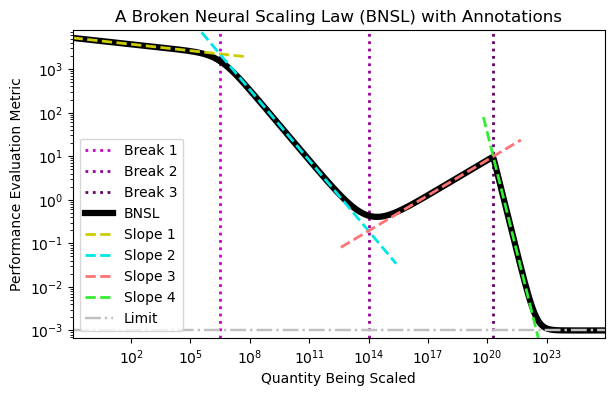
\includegraphics[width=0.7\textwidth]{figures/figure_1/figure_1.png}
%\hspace*{-.04cm}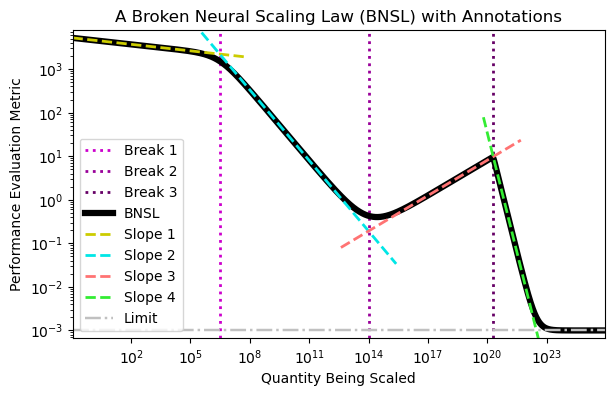
\includegraphics[width=0.815\textwidth]{figures/figure_1/figure_1__wide.png}
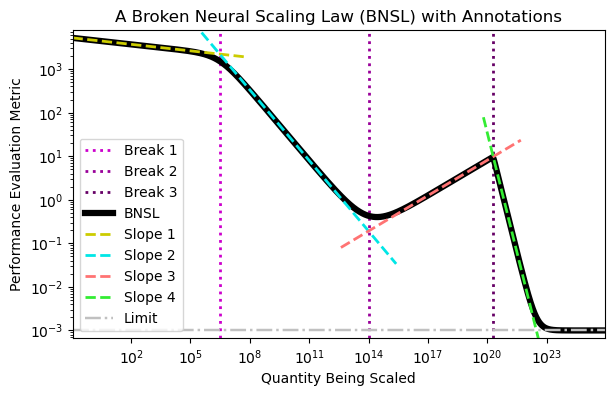
\includegraphics[width=1.0\textwidth]{figures/figure_1/figure_1__wide.png}
%\vspace{-4.7mm}

    %\caption{A Broken Neural Scaling Law (BNSL) (dark black solid line) with 3 breaks (where purple dotted lines intersect with dark black solid line) decomposed into the individual power laws (dashed lines that are yellow, blue, red, and green) that it is composed of overlaid on top of it. The 1st and 2nd break are very smooth; the 3rd break is very sharp. See Section \ref{section:bnsl} for more details. }
    %\caption{A Broken Neural Scaling Law (BNSL) (dark black solid line) with 3 breaks (where purple dotted lines intersect with dark black solid line). The individual power law segments that the BNSL contains are the regions in which the dashed lines that are yellow, blue, red, and green overlay the dark black solid line. The 1st and 2nd break are very smooth; the 3rd break is very sharp. See Section 2 for more details.}
    \caption{A Broken Neural Scaling Law (BNSL) (dark black solid line) (with 3 breaks where purple dotted lines intersect with dark black solid line) that contains 4 individual power law segments (where the dashed lines that are yellow, blue, red, and green overlap with the dark black solid line). The 1st and 2nd break are very smooth; the 3rd break is very sharp. See Section 2 for more details.}
    \label{fig:figure_1}
\end{figure*}

%\todo[inline]{TODO: Add figure 1 from \url{https://colab.research.google.com/drive/1V7PdLqRoiJGyNT0UBOq3_PuDxg2OJXv0}}

%\todo[inline]{maybe replace c and $g_i$ with $c_0$ and $c_i$ respectively}

%\vspace{-2.2mm}

The general functional form of a broken neural scaling law (BNSL) is given as follows:
%\begin{equation}
%y = \left(\frac{a}{x}\right)^b \left(1 + %\left(\frac{x}{c}\right)^d\right)^{-f} + g
%\label{eq:BNSL}
%\end{equation}
% \begin{equation}
% y = \left(\frac{a}{x}\right)^b \left(1 + \left(\frac{x}{c}\right)^d\right)^{-f} \left(1 + \left(\frac{x}{c}\right)^d\right)^{-f} + g
% \label{eq:BNSL}
% \end{equation}
%\todo[inline]{ How to best communicate that elements of equation 1 are added and removed based on number of breaks (see below)}
\begin{equation}
%\vspace{-0.05in}
%y =  a + \left(\frac{b}{x}\right)^c \prod_{i=1}^n \left(1 + \left(\frac{x}{d_i}\right)^{f_i}\right)^{-g_i},
%original version
%y =  a + \bigg(bx^{-c}\bigg) \prod_{i=1}^n \left(1 + \left(\frac{x}{d_i}\right)^{f_i}\right)^{-g_i},
%y =  a + \bigg(bx^{-c}\bigg) \prod_{i=1}^n \left(1 + \left(\frac{x}{d_i}\right)^{1/f_i}\right)^{-g_i * f_i},
y =  a + \bigg(bx^{-c_0}\bigg) \prod_{i=1}^n \left(1 + \left(\frac{x}{d_i}\right)^{1/f_i}\right)^{-c_i * f_i},
%y =  a + \Big(bx^{-c}\Big) \prod_{i=1}^n \left(1 + \left(\frac{x}{d_i}\right)^{f_i}\right)^{-g_i},
\label{eq:BNSL}
%\vspace{-0.05in}
\end{equation}
\begin{comment}
\iffalse
When $a = 0$, applying logarithms to both sides yields:
\begin{equation}
\log (y) =  c \log (b) - c \log(x) -  \sum_{i=1}^n g_i \log\left(1 + \left(\frac{x}{d_i}\right)^{f_i}\right).
%\label{eq:BNSL}
\end{equation}
TODO: I (David) made the above to try and get more intuition on this.  I guess it's not actually piece-wise linear (hence the SMOOTHLY broken)?
\fi
\end{comment}
%\begin{equation}
%y =  a + b^{-c} \prod_{i=1}^n \left(1 + {d_i}{x}^{-f_i}\right)^{-g_i}
%\label{eq:BNSL}
%\end{equation}
%In equation \ref{eq:BNSL}, 
where $y$ represents the performance evaluation metric (e.g. prediction error, cross entropy, calibration error, AUROC, BLEU score percentage, F1 score, reward, Elo rating, or FID score) (\textbf{downstream or upstream}) and $x$ represents a quantity that is being scaled (e.g. number of model parameters, amount of compute used for training, training dataset size, model input size, number of training steps, or upstream performance). The remaining  parameters %variables 
%$a, b, c, d_1 ...  d_n, f_1 ... f_n, g_1 ... g_n$
$a, b, c_0, c_1 ... c_n, d_1 ...  d_n, f_1 ... f_n$
are unknown constants that must be estimated by fitting the above functional form to the $(x,y)$ data points. (In our experiments,  SciPy curve-fitting library \citep{virtanen2020scipy} was used.) 
%are all constants that are fit via curve fitting libraries such as SciPy \cite{virtanen2020scipy}.

\iffalse
When $a = 0$, applying logarithms to both sides yields:
\begin{equation}
\log (y) =  c \log (b) - c \log(x) -  \sum_{i=1}^n g_i \log\left(1 + \left(\frac{x}{d_i}\right)^{f_i}\right).
%\label{eq:BNSL}
\end{equation}
TODO: I (David) made the above to try and get more intuition on this.  I guess it's not actually piece-wise linear (hence the SMOOTHLY broken)?
\fi

%\vspace{-38pt}
%\vspace{-20mm}

% $b = random\_guessing\_per\hspace{-.6mm}f\hspace{-.6mm}ormance - a$
% $random\_guessing\_per\hspace{-.6mm}f\hspace{-.6mm}ormance = b + a$
% $b = (random\_guessing\_per\hspace{-.6mm}f\hspace{-.6mm}ormance - a)$

%\addtolength{\topmargin}{-15mm}

The constants in equation \ref{eq:BNSL} are interpreted as follows. Constant $n$ represents the number of (smooth) ``breaks" (i.e. transitions) between $n+1$ consecutive approximately linear (on a log-log plot) segments, for a total of $n+1$  approximately linear segments (on a log-log plot); 
when $n=0$, equation \ref{eq:BNSL} becomes $y=a+bx^{-c_0}$.
%Namely, this function is approximately piece-wise linear, since the  transitions between the linear segment are smoothly interpolated, unlike the non-smooth break points in  standard piece-wise linear functions.  
%A ``break" is defined as a transition between an interval that forms a straight line on a log-log plot and another interval that forms a straight line on a log-log plot.
%The graph of this function (in a log-log plot) is not exactly piece-wise linear; instead, it smoothly interpolates between the different approximately linear regions. 
%\todo{why is that good? possible answer: intuitively, any  smooth function (in log-log) can be approximated by a piece-wise linear function with a sufficient number of smoothly connected segments - the challenge is to find how many are needed.}
%Most of our experiments use $n=1$, but we also show that 
%TODO: explain that there are varying number of variables $d_i, f_i, g_i$ depending on the number of breaks in the functional form.
Constant $a$ represents the limit as to how far the value of $y$ (performance evaluation metric) can be reduced (or maximized) even if $x$ (the quantity being scaled) goes to infinity. Constant $b$ represents the offset of functional form on a log-log plot (analogous to the intercept $b$ in $y=mx+b$ on a linear-linear plot). Constant $c_0$ represents the slope of the first approximately linear region on a log-log plot. If there is a ``slope $=0$'' random guessing region \textbf{(often there is not)} at the beginning of the scaling behavior, $c_0=0$ and $random\_guessing\_per\hspace{-.6mm}f\hspace{-.6mm}ormance = b + a$. Constant $c_i$ represents the difference in slope of the $(i)$th approximately linear region and $(i+1)$th approximately linear region on a log-log plot. Constant $d_i$ represents where on the x-axis the break between the $(i)$th and the $(i+1)$th approximately linear region (on a log-log plot) occurs. %Constant $f_i$ represents the slope of the $(i+1)$th linear region on a log-log plot. Constant $g_i$ represents the sharpness of break between the $(i)$th and the $(i+1)$th linear region on a log-log plot.
Constant $f_i$ represents the sharpness of break between the $(i)$th and the $(i+1)$th approximately linear region on a log-log plot; smaller (nonnegative) values of $f_i$ yield a sharper break and intervals (before and after the $(i)$th break) that are more linear on a log-log plot; larger values of $f_i$ yield a smoother break and intervals (before and after the $(i)$th break) that are less linear on a log-log plot.

%\vspace{-1.5mm}

For mathematical analysis and explanation of why Equation ~\ref{eq:BNSL} is smoothly piece-wise (approximately) linear function on a log-log plot, see Appendix ~\ref{section:bnsl_analysis}. For mathematical decomposition of Equation ~\ref{eq:BNSL} into the power law segments it is composed of (e.g. as in Figure \ref{fig:figure_1}), see Appendix ~\ref{section:decomposition_of_BNSL}.

%\vspace{-1.4mm}

%Note that, while an intuition for using such smoothly connected approximately piece-wise linear (in log-log plot) function was that, with enough segments, it could fit well any smooth univariate scaling function, it remained unclear whether BNSL would also {\em extrapolate} well; yet as we demonstrate below, it extrapolates quite accurately. Additionally, we find that the number of breaks needed to accurately model an entire scaling behavior is often quite small.

Note that, a smoothly connected approximately piece-wise linear (in log-log plot) function such as BNSL can, with enough segments, fit well any smooth univariate function. However, it remained unclear whether BNSL would also {\em extrapolate} the scaling behaviors of deep neural networks well; yet as we demonstrate below, it extrapolates quite accurately. Additionally, we find that the number of breaks needed to accurately model an entire scaling behavior is often quite small.

%TODO: note that equation \ref{eq:BNSL} works fine for upstream scaling too; we just name paper downstream scaling to emphasize the scenarios (i.e. downstream scaling) in which all its terms become necessary.

%\be
%\label{eq:PowerLawPlusConstant}
%L(x) = L_\infty + \left( \frac{x_0}{x}  \right)^{\alpha_x} 
%\ee

% \todo[inline]{this paragraph goes elsewhere} 
% We show mathematically and empirically that previous functional forms are unable to express inflection points, and we show mathematically and empirically that our functional form is able to express inflection points.



%We show that the functional form $y=a+(b/(x+c))^d$ (equation 1) very accurately fits 75\% of downstream tasks from the GPT-3 arXiv paper.


%When the best fit of equation 1 converges to values of d much larger than 1, the functional form equation 1 seems to not be sufficient and will probably need to be replaced with a new functional form.

%We find that the functional form $y=a+(b/((1+h)^x+c))^d$ (equation 2) is capable of fitting a subset of the downstream tasks (the downstream tasks for which equation 1 converges to values of d much larger than 1). However, equation 2 is much harder to fit due to small changes in h drastically changing y.


\iffalse
\begin{figure*}[t!]
\centering
\includegraphics[width=1.0\columnwidth]{figures/inflection_points/Two_Digit_Addition_Zero-Shot_Zoom.png}
\includegraphics[width=1.0\columnwidth]{figures/inflection_points/Two_Digit_Addition_Zero-Shot.png}
\caption{
Black points are test errors at various model sizes (numbers of parameters). Red line is functional form from equation \ref{eq:BNSL} fit to the black points. Left figure is zoomed in version of right figure. Task is Downstream Two Digit Addition (Zero-Shot) from \citet{brown2020language}. %\citet{2020arXiv200514165B}. 
All plots axes are \textbf{linear-linear} (not log-log).
}
\label{fig:Inflection_Point_example}
\end{figure*}
\fi


\iffalse
Our downstream forecasts show that an infinitely large (simultaneously infinitely deep and infinitely wide) GPT trained using the same 300 billion tokens as GPT-3 does not surpass human performance on any downstream task when using the few-shot in-context learning methodology from GPT-3 paper.
The one exception is fake news generation, for which our downstream forecast shows that humans would rate news articles generated by the model to be better than human written news articles 54.37\% of the time.

We perform ablations on the number of points and maximum of the points used for the fitting the scaling law functional form. These ablations provide some intuitions for how much to trust our forecasts.
\fi


%\section{Related Work}
To the best of our knowledge,\citet{cortes1994learning} was the first paper to model the scaling of multilayer neural network's performance as a power law 
%(also known as a scaling law) (plus a constant) \ir{[I would delete both those phrases in ()] } 
of the form $y=ax^b + c$ in which $x$ refers to training dataset size and $y$ refers to test error.
Later, \citet{2017arXiv171200409H} showed that this functional form holds over many orders of magnitude, while \citet{DBLP:journals/corr/abs-1909-12673} demonstrated  that the same functional form applies when $x$ refers to model size (number of parameters). \citet{icm2020arXiv200108361K} brought ``neural" scaling laws to the mainstream and showed that there is an additional scaling law with respect to compute. \citet{DBLP:journals/corr/abs-2106-04560} introduced the functional form $y=a(x+d)^b + c$, where  d represents the scale at which the performance starts to improve beyond the  random guess loss (a constant) and transitions to a  power law scaling regime. \citet{abnar2021exploring} proposed a functional form that relates downstream performance to upstream performance. \citet{Alabdulmohsi2022revisiting} proposed functional form $(y - \epsilon_{\infty}) / ((\epsilon_{0} - y)^a) = bx$ for relating scale to performance and released a scaling laws benchmark dataset that we use in section 

%\todo[inline]{NEED TO TALK ABOUT HOW EQUATION 6.1 OF SCALING LAWS FOR TRANSFER (plus a trivial constant for irreducible entropy) IS MATHEMATICALLY EQUIVALENT TO BNSL}

Smoothly broken power law functional forms equivalent to equation \ref{eq:UniversalScalingLaw} are common in the astrophysics literature (e.g. \cite{dampe2017direct}), but have not been used to fit scaling data in machine learning.
%\citet{2021arXiv210201293H}  - this has full list of authors/too long/not the format used in biblio for a conference
\citet{brown2020language}
described a smoothly broken power law functional form (consisting of 5 constants after reducing redundant variables) in equation 6.1 of their paper to relate scale and downstream performance. 
This is mathematically equivalent to our BNSL with a single break; however: (i) they proposed it only in the specific context of how fine-tuning plus transfer learning scales as a function of the model size. Their functional form contains a break only with respect to the number of model parameters but not with the dataset size; (ii) they only mentioned this equation in passing and do not attempt to fit any data using this functional form; (iii) they arrived at it simply via combining the scaling law for transfer that is the focus of their work with a scaling law for pretraining data, (iv) they did not identify it as a smoothly broken power law, or note any qualitative advantages of this functional form. (v) they do not talk about the family of functional forms with multiple breaks. 

%but to the best of our knowledge have never been mentioned or utilized in any literature that involves artificial neural networks.


TODO: Maybe mention "Limits of Large-Scale Training" Function
%TODO: mention that \citet{DBLP:journals/corr/abs-1909-12673} attempts to model transition from random guessing to power law
%TODO: explain why a,b,c,d are all non-negative.

%\vspace{-4.6mm}
\section{Related Work}
%\vspace{-4.8mm}
To the best of our knowledge, \citet{cortes1994learning} was the first paper to model the scaling of multilayer neural network's performance as a power law (also known as a scaling law) (plus a constant)
%(also known as a scaling law) (plus a constant) \ir{[I would delete both those phrases in ()] } 
of the form $y=ax^b + c$ in which $x$ refers to training dataset size and $y$ refers to test error; we refer to that functional form as M2. \citet{2017arXiv171200409H} showed that the functional form, M2, holds over many orders of magnitude. \citet{DBLP:journals/corr/abs-1909-12673} demonstrated  that the same functional form, M2, applies when $x$ refers to model size (number of parameters). \citet{icm2020arXiv200108361K} brought ``neural" scaling laws to the mainstream and demonstrated that the same functional form, M2, applies when $x$ refers to the amount of compute used for training. \citet{abnar2021exploring} proposed to use the same functional form, M2, to relate downstream performance to upstream performance. \citet{DBLP:journals/corr/abs-2106-04560} and \cite{bansal2022data} introduced the functional form $y=a(x+d)^b + c$, (referred to by us as M3) where  $d$ represents the scale at which the performance starts to improve beyond the  random guess loss (a constant) and transitions to a  power law scaling regime. \citet{Alabdulmohsi2022revisiting} proposed functional form $(y - \epsilon_{\infty}) / ((\epsilon_{0} - y)^a) = bx^c$, (referred to by us as M4) where  $\epsilon_{\infty}$ is irreducible entropy of the data distribution and $\epsilon_{0}$ is random guess performance, for relating scale to performance and released a scaling laws benchmark dataset that we use in our experiments. %in section 

%\vspace{-1.2mm}

%\todo[inline]{NEED TO TALK ABOUT HOW EQUATION 6.1 OF SCALING LAWS FOR TRANSFER (plus a trivial constant for irreducible entropy) IS MATHEMATICALLY EQUIVALENT TO BNSL}

%\citet{2021arXiv210201293H}  - this has full list of authors/too long/not the format used in biblio for a conference
%\citet{brown2020language}
\citet{2021arXiv210201293H} described a smoothly broken power law functional form (consisting of 5 constants after reducing redundant variables) in equation 6.1 of their paper, when relating scale and downstream performance. 
While this functional form can be summed with an additional constant representing unimprovable performance to obtain a functional form whose expressivity is equivalent to our BNSL with a single break, it is important to note that (i) \citet{2021arXiv210201293H} describes this form  only in the specific context, when exploring how  fine-tuning combined with transfer learning scales as a function of the model size - thus, their functional form contains a break only with respect to number of model parameters but not with respect to other input quantities which we do explore such as dataset size, amount of compute, and upstream performance; (ii) \citet{2021arXiv210201293H} mentioned this equation in passing and as a result did not try to fit or verify this functional form on any data; (iii) they arrived at it simply via combining the scaling law for transfer (that was the focus of their work) with a scaling law for pretraining data; (iv) they did not identify it as a smoothly broken power law, or note any qualitative advantages of this functional form; (v) they did not discuss the family of functional forms with multiple breaks. 

%\vspace{-1.6mm}

Finally, we would like to mention that smoothly broken power law functional forms, equivalent to equation \ref{eq:BNSL}, are commonly used in the astrophysics literature (e.g. \cite{dampe2017direct}) as they happen  to  model well a variety of physical phenomena. This inspired us to investigate their applicability to a wide range of deep neural scaling phenomena as well.


\clearpage


%but to the best of our knowledge have never been mentioned or utilized in any literature that involves artificial neural networks.


%TODO: Maybe mention "Limits of Large-Scale Training" Function
%TODO: mention that \citet{DBLP:journals/corr/abs-1909-12673} attempts to model transition from random guessing to power law
%TODO: explain why a,b,c,d are all non-negative.


%\section{Theoretical Limitations of Other Scaling Laws}

%\todo[inline]{I'm not sure it's worth including any propositions in the main text.  The proofs are just basic calculus and algebra.}


%\todo[inline]{This is for M2.  Need to do M3 (and maybe M4) case as well.  Also need to know which one(s) to consider "standard" for framing.}

Our use of BNSLs is inspired by the observation that scaling is not always well predicted by a simple power law.
Nor are the modifications which have been applied in previous works sufficient to capture the qualitative properties of empirical scaling curves.  
In effect, the most sophisticated form common in previous work is a power law modified to incorporate a minimum achievable loss, representing irreducible entropy, and TODO.
Here we show mathematically two qualitative defects of these functional forms:
\begin{enumerate}
    \item They are strictly monotonic and thus unable to fit double descent phenomena.
    \item They cannot express inflection points, which are frequently observed empirically.
\end{enumerate}
%This can be seen by observing that thes
Note that these functional forms \textit{can} exhibit inflection points on the log-log axes which are commonly used for plotting scaling data.  
However, on a linear-linear plot, the extra expressiveness of broken neural scaling laws is required (and sufficient).
Figure~\ref{fig:double_descent} and Figure~\ref{fig:arithmetic}, provides examples of BNSLs (with a single break-point, $n=1$) producing double descent and inflection points, respectively, establishing the capacity of this functional form to fit these phenomena.

We now explain why standard functional forms are incapable of exhibiting either behavior.
First, recall that expressions of the form $m^n$ can only take the value $0$ if $m=0$. 
We now examine the expressions for the first and second derivatives of M1, M2, M3, M3', provided in Table~\ref{tab:math}, and observe that they are all continuous and do not have roots over the relevant ranges of $a,b,c,d,x>0$, $b<1$.
This implies that they are monotonic (as the first derivative never changes sign), and that they lack inflection points (since an inflection point must have $f''(x)=0$).

\begin{table}[h]
\centering
\begin{tabular}{c|c|c|c}
name & $f(x)$ & $f'(x)$ & $f''(x)$ \\
\midrule
M1  & $ax^b$ & $abx^{b-1}$ & $ab(b-1)x^{b-2}$ \\
\midrule
M2  & $ax^b + c$ & $abx^{b-1}$ & $ab(b-1)x^{b-2}$ \\
%M2  & $f(x)$ & $f'(x)$ & $\frac{(c (1 + c) (b/x)^c)}{x^2}$ \\
\midrule
M3  & $a(x^{-1} + d)^{-b} + c$  & 
%$\frac{a b }{x (1 + d x)(d + 1/x)^{b}}$  & $a b x^{(b-2)} (1 + d x)^{(-2 - b)} (b -1 - 2 d x) $ \\
$a b  x^{(b-1)} (1 + d x)^{(-1 - b)}$  & $a b x^{(b-2)} (1 + d x)^{(-2 - b)} (b -1 - 2 d x) $ 
% \midrule
% M3' & $f(x)$ & $f'(x)$ & $f''(x)$ \\
%The above expression does not have a root for $a,b,d,x>0; b < 1$: the first two terms are strictly positive, meaning we would need $b = 2dx + 1 \geq 1$.
\label{tab:math}
\end{tabular}
\caption{
    Previously proposed functional forms and their (first and second order) derivatives.  
    For $a,b,c,d,x>0$, $b<1$, the expressions for each of the derivatives is a product of non-zero multiplicands, and thus none of these functional forms can express functions that are non-monotonic or have inflection points.
    %The above expression does not have a root for $a,b,d,x>0; b < 1$: the first two terms are strictly positive, meaning we would need $b = 2dx + 1 \geq 1$.
 }
\end{table}


Figure \ref{fig:Inflection_Point_example} is an example of this inflection point present in experimental data from a real world downstream task, Two Digit Addition (Zero-Shot) from \citet{brown2020language}. %\citet{2020arXiv200514165B}. 
In the small scale regime, the function is concave downward as it transitions from random guessing performance to starting to learn the task. As the scale increases past the small scale regime, an inflection point is reached and the function becomes concave upward as power law scaling behaviour takes over.



% % M3: (need d>0) 
% M3: $f(x) = a(x^{-1} + d)^{-b} + c$ 
% $$
%  f'(x) = \frac{a b }{x (1 + d x)(d + 1/x)^{b}} 
% $$
% $$
%  f''(x) = a b x^{(b-2)} (1 + d x)^{(-2 - b)} (b -1 - 2 d x) 
% $$
% The above expression does not have a root for $a,b,d,x>0; b < 1$: the first two terms are strictly positive, meaning we would need $b = 2dx + 1 \geq 1$.

% "also M3?": $f(x)=a(x+d)^b + c$
% $$
% f'(x) = a b (d + x)^{(b-1)}
% $$
% $$
% f''(x) = a (-1 + b) b (d + x)^{(b-2)}
% $$
% Neither of the above expressions have roots because they are a product of non-zero constants and expressions of the form $m^n$.


%M2: $y = ax^b +c$


% \subsection{SCRAPS}

% % TODO: convert this to same form as M2
% \begin{proposition}
%     Functions of the form $f(x) = a + \left(\frac{b}{x}\right)^c$ are necessarily monotonic for $a,b,c>0$ in the range $x>0$.
% \end{proposition}
% \begin{proof}
%     A sufficient condition for monotonicity is that $f'(x)$ does not change sign.  
%     In our case, we have 
%     $$
%     f'(x) = - bc \left(\frac{b}{x}\right)^{(c-1)}.
%     $$
%     Since $b$ and $x$ are both positive, so is the ratio $\frac{b}{x}$.  
%     And since a positive number taken to any power is also positive, the entire expression is guaranteed to be negative for all values of $a,b,c,x>0$.
% \end{proof}

% %TODO: rename this section to "Math Proofs" and also prove that other functional forms can't express non-monotonic behavior

% \begin{proposition}
%     Functions of the form $f(x) = a + \left(\frac{b}{x}\right)^c$ cannot contain an inflection point for $a,b,c>0$ in the range $x>0$.
% \end{proposition}
% \begin{proof}
% The second derivative is:
% $$
% f''(x) = 
% \frac{(c (1 + c) (b/x)^c)}{x^2}.
% $$
% Since $b$, $c$ and $x$ are all positive, all of the multiplicands of $f''(x)$ are positive, and thus so is $f''(x)$, but an inflection point must have $f''(x)=0$.
% \end{proof}

% \subsection{SCRAPS}

% An inflection point is a point of a curve at which the second order derivative (i.e.\ curvature) changes signs. 
% Empirically, the function relating the performance evaluation metric (e.g. prediction error) to the quantity being scaled (e.g.\ model size) often has an inflection point. 
% Figure \ref{fig:Inflection_Point_example} is an example of this inflection point present in experimental data from a real world downstream task, Two Digit Addition (Zero-Shot) from \citet{brown2020language}. %\citet{2020arXiv200514165B}. 
% In the small scale regime, the function is concave downward as it transitions from random guessing performance to starting to learn the task. 
% As the scale increases past the small scale regime, an inflection point is reached and the function becomes concave upward as power law scaling behaviour takes over.

% However, \textbf{Proposition:} typical functional form cannot have an inflection point.
% \textbf{Proof:}
% %https://www.wolframalpha.com/input?i=d%5E2%2Fdx%5E2+%28a+%2B+%28b%2Fx%29**c%29+
% An inflection point is a point of a curve at which the second order derivative (i.e.\ curvature) changes signs. 
% The second derivative of this function is:
% $$
% f''(x) = 
% \frac{(c (1 + c) (b/x)^c)}{x^2}.
% $$
% Since $b$, $c$ and $x$ are all positive, all of the multiplicands of $f''(x)$ are positive, and thus so is $f''(x)$, but an inflection point must have $f''(x)=0$.
% % https://www.wolframalpha.com/input?i=d%5E2%2Fdx%5E2+%28a+%2B+%28b%2Fx%29**c+%281+%2F+%28x%2Bd%29%5Ef%29%29

% Note that inflection points often appear in scaling curves, which are typically plotted on log/log axes, and existing scaling laws can fit those inflection points (TODO: is this right?  I thought they were just linear on a log/log plot?).
% Inflection points are less common but still sometimes present in a linear/linear plot; These are the inflection points that existing scaling laws cannot capture.

% TODO: do we get the same result for all of M1 through M4?

% All the functional forms:

% M1: $y = ax^b$

% M2: $y = ax^b +c$

% M3: $y = a(x^{-1} + d)^{-b} + c$ 

% also M3?: $y=a(x+d)^b + c$

% M4: $(y - \epsilon_{\infty}) / ((\epsilon_{0} - y)^a) = bx$ 

% $\epsilon_{\infty}$ is irreducible loss, and $\epsilon_{0}$ is performance of random guessing.

% Equation 6.1 of "scaling laws for transfer" paper: $y = (ax^b + cx^d)^f + g$

% I (Ethan) just now have realized that this equation 6.1 above is a smoothly broken power law (i.e. mathematically equivalent to ours I think) too so we have to change the narrative of the paper now:  
% \url{https://math.stackexchange.com/a/2427151}

% \url{https://colab.research.google.com/drive/1QP81soNf1DDV_Q6iimN8sb-hZHaZeMyW}

% Also, I think "scaling laws for transfer" paper may/might have been unaware that its equation 6.1 is a thing called a smoothly broken power law.

% Broken Neural Scaling Law: $y =  a + \left(\frac{b}{x}\right)^c \prod_{i=1}^n \left(1 + \left(\frac{x}{d_i}\right)^{f_i}\right)^{-g_i}$



% TODO: remove this section?
% TODO: replace it with section about breaks rather than inflection points


%This inflection point at the transition from constant random guessing performance in the small scale regime to 
%When the performance evaluation metric (e.g. prediction error) is plotted on y-axis and the quantity being scaled (e.g. model size) is plotted on x-axis, the plotted data has an inflection point at the transition from constant random guessing performance in the small scale regime to 
% Figure \ref{fig:Inflection_Point_example} is an example of this inflection point present in experimental data from a real world downstream task, Two Digit Addition (Zero-Shot) from \citet{brown2020language}. %\citet{2020arXiv200514165B}. 
%In the small scale regime, the function is concave downward as it transitions from random guessing performance to starting to learn the task. As the scale increases past the small scale regime, an inflection point is reached and the function becomes concave upward as power law scaling behaviour takes over.

% \todo[inline]{math proofs}

% 1. proof that shows $y=a/(x^b+d)+c$ has inflection point for all functions in which $a$ $!=0$, $b>1$, and $d>0$ are simultaneously true

% 2. proof that shows $y=a(x+d)^b + c$ never has inflection point
\section{Theoretical Limitations of Previously Proposed Scaling Laws}
\label{section:math_proofs}

%\todo[inline]{I'm not sure it's worth including any propositions in the main text.  The proofs are just basic calculus and algebra.}

%\todo[inline]{This is for M2.  Need to do M3 (and maybe M4) case as well.  Also need to know which one(s) to consider "standard" for framing.}

Our use of BNSLs is inspired by the observation that scaling is not always well predicted by a simple power law;
nor are many of the modifications which have been applied in previous works sufficient to capture the qualitative properties of empirical scaling curves.  
% In effect, the most sophisticated form common in previous work is a power law modified to incorporate a minimum achievable loss, representing irreducible entropy, and TODO.
Here we show mathematically two qualitative defects of these functional forms:
\begin{enumerate}
    \item They are strictly monotonic (first-order derivative does not change its sign) and thus unable to fit double descent phenomena.
    \item They cannot express inflection points (second-order derivative does not change its sign), which are frequently observed empirically.  An exception to this is M4, proposed by \citet{Alabdulmohsi2022revisiting}. %, which can model a single inflection point.
\end{enumerate}
Note that these functional forms \textit{can} exhibit inflection points on the log-log axes which are commonly used for plotting scaling data (as it was observed in several prior works).
However, for inflection points on a \textit{linear-linear} plot, the extra expressiveness of broken neural scaling laws appears to be necessary (and sufficient).
Figure~\ref{fig:double_descent} and Figure~\ref{fig:arithmetic}, provide examples of BNSLs producing non-monotonic behavior and inflection points, respectively, establishing the capacity of this functional form to model these phenomena that occur in real scaling behavior.

\begin{table}[h]
\centering
\footnotesize
\begin{tabular}{c|c|c|c}
name & $f(x)$ & $f'(x)$ & $f''(x)$ \\
\midrule
M1  & $ax^b$ & $abx^{b-1}$ & $ab(b-1)x^{b-2}$ \\
\midrule
M2  & $ax^b + c$ & $abx^{b-1}$ & $ab(b-1)x^{b-2}$ \\
%M2  & $f(x)$ & $f'(x)$ & $\frac{(c (1 + c) (b/x)^c)}{x^2}$ \\
\midrule
M3  & $a(x^{-1} + d)^{-b} + c$  & 
$\frac{a b }{x (1 + d x)(d + 1/x)^{b}}$  & $a b x^{(b-2)} (1 + d x)^{(-2 - b)} (b -1 - 2 d x) $ \\
%$~~f(x) = g^{-1}(x)$  &   & & \\ 
%$x:=g(y)$
% \midrule
% M3' & $f(x)$ & $f'(x)$ & $f''(x)$ \\
%\midrule
%M4 &  $(y - \epsilon_{\infty}) / ((\epsilon_{0} - y)^a) = bx$ &  $f'(x)$ & $f''(x)$ \\
% M3' & $f(x)$ & $f'(x)$ & $f''(x)$ \\
%The above expression does not have a root for $a,b,d,x>0; b < 1$: the first two terms are strictly positive, meaning we would need $b = 2dx + 1 \geq 1$.
\end{tabular}
\caption{
    Previously proposed functional forms M1, M2, M3 and their (first and second order) derivatives.  See Equation~\ref{eqn:M4} for M4.
    %For $d,x>0$, $b<0$, the expressions for each of the derivatives is a product of non-zero multiplicands, and thus none of these functional forms can express functions that are non-monotonic or have inflection points.
    %The above expression does not have a root for $a,b,d,x>0; b < 1$: the first two terms are strictly positive, meaning we would need $b = 2dx + 1 \geq 1$.
 }
\label{tab:math}
\end{table}


% \begin{table}[h]
% \centering
% \footnotesize
% \begin{tabular}{c|c|c|c}
% \midrule
% $f(x) = g^{-1}(x)$ & $g(y)$ & $g'(y)$ & $g''(y)$ \\
% \midrule
% M4  & $\frac{1}{b}\big(\frac{y - \epsilon_{\infty}}{(\epsilon_{0} - y)^a}\big)^{1/c}$ &  
% $\frac{((\epsilon_0 - y)^{-a} + a (\epsilon_0 - y)^{-1 - a} (y - \epsilon_{\infty})) ((\epsilon_0 - y)^{-a} (y - \epsilon_{\infty}))^{1/c - 1})}{b c}$ &  \\
% %$\frac{-a (y - \epsilon_{0})^{(-a - 2)} (\epsilon_{\infty} + a \epsilon_{\infty} - 2 \epsilon_{0} + y - a y)}{b}$ \\
% \end{tabular}
% \caption{
%     Previously proposed functional forms and their (first and second order) derivatives.  
%     %For $d,x>0$, $b<0$, the expressions for each of the derivatives is a product of non-zero multiplicands, and thus none of these functional forms can express functions that are non-monotonic or have inflection points.
%     %The above expression does not have a root for $a,b,d,x>0; b < 1$: the first two terms are strictly positive, meaning we would need $b = 2dx + 1 \geq 1$.
%  }
% \label{tab:math}
% \end{table}
%\end{tiny}
%\FloatBarrier

%\todo[inline]{TODO: fix claims of this section; and make sure claims everywhere in paper agree with claims here}

\noindent{\bf M1, M2, M3 functional forms cannot model non-monotonic behavior or inflection points:}  %We now explain why standard functional forms are incapable of exhibiting either behavior.
First, recall that expressions of the form $m^n$ can only take the value $0$ if $m=0$. 
We now examine the expressions for the first and second derivatives of M1, M2, M3, %M3',
provided in Table~\ref{tab:math}, and observe that they are all continuous and do not have roots over the relevant ranges of their variables, i.e.\ $x>0$ in general and $b<0$ in the case of M3 
%(we require $x > 0$ because the scaling variable (such as model size, dataset size, or amount of compute used) is always non-negative).
(we require $x > 0$ because model size, dataset size, and compute are always non-negative).
This implies that, for any valid settings of the parameters $a,b,c,d,x$, these functional forms are monotonic (as the first derivative never changes sign), and that they lack inflection points (since an inflection point must have $f''(x)=0$).

\noindent{\bf M4 functional form cannot model non-monotonic behavior.}  %We now 
The case of M4 is a bit different, since the relationship between $y$ and $x$ in this case is expressed as an inverse function, i.e.
\begin{align}
\label{eqn:M4}
x = g(y) = \left(\frac{y - \epsilon_{\infty}} {b(\epsilon_{0} - y)^a}\right)^{1/c}
\end{align}
However, non-monotonicity of $y$ as an inverse function $y = g^{-1}(x)$ is ruled out, since that would imply two different values of $x=g(y)$ can be obtained for the single value of $y$ -- this is impossible, since $f(y)$ maps each $y$ deterministically to a single value of $x$. As a result, M4 cannot express non-monotonic functions.
%As to the possibility of modeling an inflection point, we were yet not able to determine whether M4 has this capability or not.
%$a, b,c,e_0,e_{inf} = 1, 1, -2, .75, .25.$

\noindent{\bf M4 functional form can model inflection points.}  %We now 
%M4 is capable of expressive inflection points, however. 
It is easy to see that if $y=g^{-1}(x)$ had an inflection point, then $x = g(y)$ would have it as well. This is because an inflection point is defined as a point $x$ where $f(x)$ changes from concave to convex, which implies that $g(y)$ changes from convex to concave, since the inverse of a convex function is concave; the root(s) of $g''(y)$ are the point(s) at which this change occurs.
Using Wolfram Alpha\footnote{\href{https://www.wolframalpha.com/}{https://www.wolframalpha.com/}} and matplotlib \citep{Hunter:2007}, we observe that M4 is able to express inflection points, e.g.\ $(a,b,c,\epsilon_0, \epsilon_{\infty}, x, y) = (1,1,-2,3/4,1/4,1/\sqrt3, 5/8$), or $(a,b,c,\epsilon_0, \epsilon_{\infty}, x, y) = (2,1,-3,2/3,1/3,(-5/6 + \sqrt3/2)^{1/3}, 1/\sqrt3)$. % TODO: double check these (ideally someone else does that, to be extra sure)



% meaning M4 is capable of expressing an inflection point.
% Note also that when $a=1$, we can solve for M4 for $y$ in closed form, yielding the expression $y = \frac{h + j(bx)^c} {1 + (bx)^c}$.

%For $g''(y)$ to have a root we would need $y = (1-a) ((1+a)\epsilon_\infty - 2 \epsilon_0) =0 $; This can be achieved for $a=2, \epsilon_\infty=2/3, \epsilon_0=1$. 


% but this is impossible because we have $0 <\epsilon_\infty \leq \epsilon_0  < 1$ and $0<a<1$.
%However, it is easy to show via simple algebraic computation that  second derivative $g''(y)$ never equals zero, thus ruling out the possibility of inflection points with this functional form as well.

%\FloatBarrier
%\begin{tiny}



%Figure \ref{fig:Inflection_Point_example} is an example of this inflection point present in experimental data from a real world downstream task, Two Digit Addition (Zero-Shot) from \citet{brown2020language}. %\citet{2020arXiv200514165B}. 
%In the small scale regime, the function is concave downward as it transitions from random guessing performance to starting to learn the task. As the scale increases past the small scale regime, an inflection point is reached and the function becomes concave upward as power law scaling behaviour takes over.



% % M3: (need d>0) 
% M3: $f(x) = a(x^{-1} + d)^{-b} + c$ 
% $$
%  f'(x) = \frac{a b }{x (1 + d x)(d + 1/x)^{b}} 
% $$
% $$
%  f''(x) = a b x^{(b-2)} (1 + d x)^{(-2 - b)} (b -1 - 2 d x) 
% $$
% The above expression does not have a root for $a,b,d,x>0; b < 1$: the first two terms are strictly positive, meaning we would need $b = 2dx + 1 \geq 1$.

% "also M3?": $f(x)=a(x+d)^b + c$
% $$
% f'(x) = a b (d + x)^{(b-1)}
% $$
% $$
% f''(x) = a (-1 + b) b (d + x)^{(b-2)}
% $$
% Neither of the above expressions have roots because they are a product of non-zero constants and expressions of the form $m^n$.


%M2: $y = ax^b +c$


% \subsection{SCRAPS}

% % TODO: convert this to same form as M2
% \begin{proposition}
%     Functions of the form $f(x) = a + \left(\frac{b}{x}\right)^c$ are necessarily monotonic for $a,b,c>0$ in the range $x>0$.
% \end{proposition}
% \begin{proof}
%     A sufficient condition for monotonicity is that $f'(x)$ does not change sign.  
%     In our case, we have 
%     $$
%     f'(x) = - bc \left(\frac{b}{x}\right)^{(c-1)}.
%     $$
%     Since $b$ and $x$ are both positive, so is the ratio $\frac{b}{x}$.  
%     And since a positive number taken to any power is also positive, the entire expression is guaranteed to be negative for all values of $a,b,c,x>0$.
% \end{proof}

% %TODO: rename this section to "Math Proofs" and also prove that other functional forms can't express non-monotonic behavior

% \begin{proposition}
%     Functions of the form $f(x) = a + \left(\frac{b}{x}\right)^c$ cannot contain an inflection point for $a,b,c>0$ in the range $x>0$.
% \end{proposition}
% \begin{proof}
% The second derivative is:
% $$
% f''(x) = 
% \frac{(c (1 + c) (b/x)^c)}{x^2}.
% $$
% Since $b$, $c$ and $x$ are all positive, all of the multiplicands of $f''(x)$ are positive, and thus so is $f''(x)$, but an inflection point must have $f''(x)=0$.
% \end{proof}

% \subsection{SCRAPS}

% An inflection point is a point of a curve at which the second order derivative (i.e.\ curvature) changes signs. 
% Empirically, the function relating the performance evaluation metric (e.g. prediction error) to the quantity being scaled (e.g.\ model size) often has an inflection point. 
% Figure \ref{fig:Inflection_Point_example} is an example of this inflection point present in experimental data from a real world downstream task, Two Digit Addition (Zero-Shot) from \citet{brown2020language}. %\citet{2020arXiv200514165B}. 
% In the small scale regime, the function is concave downward as it transitions from random guessing performance to starting to learn the task. 
% As the scale increases past the small scale regime, an inflection point is reached and the function becomes concave upward as power law scaling behaviour takes over.

% However, \textbf{Proposition:} typical functional form cannot have an inflection point.
% \textbf{Proof:}
% %https://www.wolframalpha.com/input?i=d%5E2%2Fdx%5E2+%28a+%2B+%28b%2Fx%29**c%29+
% An inflection point is a point of a curve at which the second order derivative (i.e.\ curvature) changes signs. 
% The second derivative of this function is:
% $$
% f''(x) = 
% \frac{(c (1 + c) (b/x)^c)}{x^2}.
% $$
% Since $b$, $c$ and $x$ are all positive, all of the multiplicands of $f''(x)$ are positive, and thus so is $f''(x)$, but an inflection point must have $f''(x)=0$.
% % https://www.wolframalpha.com/input?i=d%5E2%2Fdx%5E2+%28a+%2B+%28b%2Fx%29**c+%281+%2F+%28x%2Bd%29%5Ef%29%29

% Note that inflection points often appear in scaling curves, which are typically plotted on log/log axes, and existing scaling laws can fit those inflection points (TODO: is this right?  I thought they were just linear on a log/log plot?).
% Inflection points are less common but still sometimes present in a linear/linear plot; These are the inflection points that existing scaling laws cannot capture.

% TODO: do we get the same result for all of M1 through M4?

% All the functional forms:

% M1: $y = ax^b$

% M2: $y = ax^b +c$

% M3: $y = a(x^{-1} + d)^{-b} + c$ 

% also M3?: $y=a(x+d)^b + c$

% M4: $(y - \epsilon_{\infty}) / ((\epsilon_{0} - y)^a) = bx$ 

% $\epsilon_{\infty}$ is irreducible loss, and $\epsilon_{0}$ is performance of random guessing.

% Equation 6.1 of "scaling laws for transfer" paper: $y = (ax^b + cx^d)^f + g$

% I (Ethan) just now have realized that this equation 6.1 above is a smoothly broken power law (i.e. mathematically equivalent to ours I think) too so we have to change the narrative of the paper now:  
% \url{https://math.stackexchange.com/a/2427151}

% \url{https://colab.research.google.com/drive/1QP81soNf1DDV_Q6iimN8sb-hZHaZeMyW}

% Also, I think "scaling laws for transfer" paper may/might have been unaware that its equation 6.1 is a thing called a smoothly broken power law.

% Broken Neural Scaling Law: $y =  a + \left(\frac{b}{x}\right)^c \prod_{i=1}^n \left(1 + \left(\frac{x}{d_i}\right)^{f_i}\right)^{-g_i}$



% TODO: remove this section?
% TODO: replace it with section about breaks rather than inflection points


%This inflection point at the transition from constant random guessing performance in the small scale regime to 
%When the performance evaluation metric (e.g. prediction error) is plotted on y-axis and the quantity being scaled (e.g. model size) is plotted on x-axis, the plotted data has an inflection point at the transition from constant random guessing performance in the small scale regime to 
% Figure \ref{fig:Inflection_Point_example} is an example of this inflection point present in experimental data from a real world downstream task, Two Digit Addition (Zero-Shot) from \citet{brown2020language}. %\citet{2020arXiv200514165B}. 
%In the small scale regime, the function is concave downward as it transitions from random guessing performance to starting to learn the task. As the scale increases past the small scale regime, an inflection point is reached and the function becomes concave upward as power law scaling behaviour takes over.

% \todo[inline]{math proofs}

% 1. proof that shows $y=a/(x^b+d)+c$ has inflection point for all functions in which $a$ $!=0$, $b>1$, and $d>0$ are simultaneously true

% 2. proof that shows $y=a(x+d)^b + c$ never has inflection point


%\section{Functional Form Fits and Extrapolations}
\label{section:functional_form_fits}

We now show the fits and/or extrapolations of various functional forms. In all plots here and in the appendix, black points are the points used for fitting a functional form, green points are the held-out points used for evaluating extrapolation of a functional form fit to the black points, and a red line is the BNSL that has been fit to the black points.

In the tables and elsewhere, 
\begin{itemize}
    \item M1 refers to functional form $y = ax^b$
    \item M2 refers to functional form $y = ax^b +c$
    \item M3 refers to functional form $y = a(x^{-1} + d)^{-b} + c$
    \item M4 refers to functional form $(y - \epsilon_{\infty}) / ((\epsilon_{0} - y)^a) = bx$
\end{itemize}

All the extrapolation evaluations reported in the tables are reported in terms of root mean squared log error (RMSLE\footnote{RMSLE = $ \sqrt{(\sum_{i=1}^{n} (log(y_{i})-log(\hat{y}_{i}))^2)/n}$}) ± root standard log error. 

TODO: define root standard log error; see commented out lines for how it's calculated
\[error = (log(y_{i})-log(\hat{y}_{i}))^2)\] 
\[\mu_{error} = \frac{1}{N}\sum_{i=1}^N error\]
\[\sigma_{error} = \sqrt{\frac{1}{N-1}\sum_{i=1}^N(error_i-\mu_{error})^2}\]
\[rstderr = \sqrt{\mu_{error} + \frac{\sigma_{error}}{\sqrt{len(\hat{y})}}} - \sqrt{\mu_{error}}\] 
% how root standard log error is calculated
%error = (np.log(yp) - np.log(y)) ** 2
%errmu = np.mean(error)
%rstderr = np.sqrt(errmu + np.std(error) / (len(yp)**0.5)) - np.sqrt(errmu)

\FloatBarrier
\subsection{Vision}
\label{section:scaling_benchmark__vision}

(TODO: this sentence is repeated in language section)

Using the scaling laws benchmark of \cite{Alabdulmohsi2022revisiting}, we evaluate how well various functional forms extrapolate performance on vision tasks as training dataset size increases. In this vision subset of the benchmark, the tasks that are evaluated are error rate on each of various few-shot downstream image classification (IC) tasks; the downstream tasks are: Birds 200 \cite{welinder2010caltech}, Caltech101 \cite{fei2004learning}, CIFAR-100 \cite{krizhevsky2009learning}, and ImageNet \cite{deng2009imagenet}. The following architectures of various sizes are pretrained on subsets of JFT-300M: big-transfer residual neural networks (BiT) \cite{kolesnikov2020big}, MLP mixers (MiX) \cite{tolstikhin2021mlp}, and vision transformers (ViT) \cite{dosovitskiy2020image}. As can be seen in Table  \ref{table:scaling_laws_benchmark_dataset__Vision}, BNSL (TODO: make sure BNSL abbreviation is defined somewhere) yields extrapolations with the lowest RMSLE (Root Mean Squared Logarithmic Error) for the largest number (by a very large margin) (TODO: replace "large margin" with numbers) of tasks of any of the functional forms.

To view all plots of the BNSL on each of these tasks, see figures
\ref{fig:scaling_laws_benchmark_dataset__birds},
\ref{fig:scaling_laws_benchmark_dataset__cifar_100},
\ref{fig:scaling_laws_benchmark_dataset__caltech},
\ref{fig:scaling_laws_benchmark_dataset__ImageNet} in Appendix \ref{section:Plots_of_BNSL_Extrapolations}. To view all plots of M1, M2, M3, and M4 on each of these tasks, see Appendix A.4 of \cite{Alabdulmohsi2022revisiting}.

% \begin{center}
\begin{table}
    \centering
    \begin{tabular}{ |c|c|c|c|c|c|c| } 
\hline
Domain & \hspace{.9cm}Task & M1 $\uparrow$ & M2 $\uparrow$ & M3 $\uparrow$ & M4 $\uparrow$ & BNSL $\uparrow$ \\
 \hline
 IC & Birds 200 & 0 & 0 & 0 & 5.56 & \highlight{94.44}\\ 
 IC & Caltech101 & 0 & 0 & 5.56 & 5.56 & \highlight{88.89}\\ 
 IC & CIFAR-100 & 0 & 5.56 & 5.56 & 5.56 & \highlight{83.33}\\
 IC & ImageNet & 0 & 0 & 11.11 & 0 & \highlight{88.89}\\
 Language & All & 5 & 10 & 15 & 25 & \highlight{45}\\
 \hline
\end{tabular}
    \caption{
    Percentage of tasks by domain where each functional form is the best for extrapolation. See Section \ref{section:scaling_benchmark__vision} for more details. Numbers for M1, M2, M3, and M4 were obtained via correspondence with authors of \cite{Alabdulmohsi2022revisiting}. 
    }
    \label{table:scaling_laws_benchmark_dataset__Vision}
\end{table}
% \end{center}

\begin{table}[htbp]
\tiny
% \fontsize{8}{8}\selectfont
% \setlength\tabcolsep{3.1pt} 
\begin{tabular}
%{p{.02\textwidth}p{.165\textwidth}p{.095\textwidth}p{.01\textwidth}p{.01\textwidth}p{.099\textwidth}p{.099\textwidth}p{.099\textwidth}p{.099\textwidth}p{.099\textwidth}}
{p{.205\textwidth}p{.111\textwidth}p{.099\textwidth}p{.099\textwidth}p{.099\textwidth}p{.099\textwidth}p{.099\textwidth}}
%\begin{tabular}{llllrrrrrrrrrrrrl}
\hspace{.9cm}Task & Model & M1 $\downarrow$ & M2 $\downarrow$ & M3 $\downarrow$ & M4 $\downarrow$ & BNSL $\downarrow$ \\
\hline
Birds 200 10-shot & BiT/101/3 & 9.13e-2 & 9.13e-2 & 9.13e-2 & 2.49e-2 & \highlight{3.79e-3} \\
Birds 200 10-shot & BiT/50/1 & 6.88e-2 & 6.88e-2 & 5.24e-2 & 2.48e-2 & \highlight{4.96e-3} \\
Birds 200 10-shot & MiX/B/16 & 9.15e-2 & 9.15e-2 & 3.95e-2 & 4.14e-2 & \highlight{9.98e-3} \\
Birds 200 10-shot & MiX/L/16 & 5.51e-2 & 5.51e-2 & 5.51e-2 & 4.59e-2 & \highlight{8.41e-3} \\
Birds 200 10-shot & ViT/B/16 & 6.77e-2 & 6.77e-2 & 3.52e-2 & 1.87e-2 & \highlight{9.81e-3} \\
Birds 200 10-shot & ViT/S/16 & 3.95e-2 & 3.95e-2 & 3.74e-2 & \highlight{9.81e-3} & 1.51e-2 \\
Birds 200 25-shot & BiT/101/3 & 9.41e-2 & 9.41e-2 & 9.41e-2 & 5.09e-2 & \highlight{7.24e-3} \\
Birds 200 25-shot & BiT/50/1 & 1.10e-1 & 7.29e-2 & 1.52e-2 & 1.63e-2 & \highlight{8.00e-3} \\
Birds 200 25-shot & MiX/B/16 & 1.40e-1 & 1.40e-1 & 6.93e-2 & 1.85e-2 & \highlight{5.02e-3} \\
Birds 200 25-shot & MiX/L/16 & 1.12e-1 & 1.12e-1 & 1.12e-1 & 4.88e-2 & \highlight{1.05e-2} \\
Birds 200 25-shot & ViT/B/16 & 9.02e-2 & 9.02e-2 & 3.75e-2 & 1.52e-2 & \highlight{5.87e-3} \\
Birds 200 25-shot & ViT/S/16 & 5.06e-2 & 5.06e-2 & 4.96e-2 & 3.28e-2 & \highlight{1.21e-2} \\
Birds 200 5-shot & BiT/101/3 & 8.17e-2 & 8.17e-2 & 8.17e-2 & 3.00e-2 & \highlight{6.08e-3} \\
Birds 200 5-shot & BiT/50/1 & 5.44e-2 & 5.44e-2 & 5.44e-2 & 2.63e-2 & \highlight{5.79e-3} \\
Birds 200 5-shot & MiX/B/16 & 8.27e-2 & 8.27e-2 & 5.49e-2 & 1.86e-2 & \highlight{5.74e-3} \\
Birds 200 5-shot & MiX/L/16 & 5.68e-2 & 5.68e-2 & 5.68e-2 & 2.65e-2 & \highlight{5.06e-3} \\
Birds 200 5-shot & ViT/B/16 & 3.40e-2 & 3.40e-2 & 3.40e-2 & 1.26e-2 & \highlight{6.32e-3} \\
Birds 200 5-shot & ViT/S/16 & 2.75e-2 & 2.75e-2 & 2.75e-2 & 1.56e-2 & \highlight{6.93e-3} \\
\hline
CIFAR-100 10-shot & BiT/101/3 & 8.57e-2 & 8.57e-2 & 8.25e-2 & 9.28e-2 & \highlight{1.53e-2} \\
CIFAR-100 10-shot & BiT/50/1 & 7.44e-2 & 1.24e-2 & 2.08e-2 & 1.23e-2 & \highlight{9.74e-3} \\
CIFAR-100 10-shot & MiX/B/16 & 8.77e-2 & 8.77e-2 & 2.71e-2 & 2.60e-2 & \highlight{8.61e-3} \\
CIFAR-100 10-shot & MiX/L/16 & 1.05e-1 & 1.05e-1 & 4.85e-2 & 4.76e-2 & \highlight{1.55e-2} \\
CIFAR-100 10-shot & ViT/B/16 & 8.98e-2 & 8.98e-2 & 8.98e-2 & 5.60e-2 & \highlight{1.73e-2} \\
CIFAR-100 10-shot & ViT/S/16 & 6.84e-2 & 2.11e-2 & 3.35e-2 & 2.47e-2 & \highlight{1.15e-2} \\
CIFAR-100 25-shot & BiT/101/3 & 8.77e-2 & 8.77e-2 & 4.44e-2 & 4.29e-2 & \highlight{9.32e-3} \\
CIFAR-100 25-shot & BiT/50/1 & 7.31e-2 & 2.35e-2 & 3.65e-2 & 2.36e-2 & \highlight{2.00e-2} \\
CIFAR-100 25-shot & MiX/B/16 & 1.08e-1 & 4.75e-2 & 2.10e-2 & 2.08e-2 & \highlight{8.15e-3} \\
CIFAR-100 25-shot & MiX/L/16 & 9.79e-2 & 9.79e-2 & 3.67e-2 & 2.79e-2 & \highlight{8.47e-3} \\
CIFAR-100 25-shot & ViT/B/16 & 1.07e-1 & 1.07e-1 & 6.54e-2 & \highlight{4.81e-2} & 1.20e-1 \\
CIFAR-100 25-shot & ViT/S/16 & 8.03e-2 & 2.19e-2 & 3.13e-2 & 2.19e-2 & \highlight{1.34e-2} \\
CIFAR-100 5-shot & BiT/101/3 & 5.94e-2 & 5.94e-2 & 5.94e-2 & 4.57e-2 & \highlight{1.58e-2} \\
CIFAR-100 5-shot & BiT/50/1 & 4.87e-2 & 4.87e-2 & \highlight{1.69e-2} & 4.91e-2 & 1.95e-2 \\
CIFAR-100 5-shot & MiX/B/16 & 7.07e-2 & 7.07e-2 & 2.78e-2 & 2.05e-2 & \highlight{6.77e-3} \\
CIFAR-100 5-shot & MiX/L/16 & 7.06e-2 & 7.06e-2 & 4.17e-2 & 3.14e-2 & \highlight{1.18e-2} \\
CIFAR-100 5-shot & ViT/B/16 & 6.27e-2 & 6.27e-2 & 6.27e-2 & 5.11e-2 & \highlight{1.19e-2} \\
CIFAR-100 5-shot & ViT/S/16 & 6.93e-2 & \highlight{2.84e-2} & 3.88e-2 & 3.09e-2 & 6.40e-2 \\
\hline
Caltech101 10-shot & BiT/101/3 & 3.07e-1 & 3.07e-1 & 1.51e-1 & 3.54e-2 & \highlight{6.42e-3} \\
Caltech101 10-shot & BiT/50/1 & 3.29e-1 & 7.68e-2 & 1.13e-1 & 6.31e-2 & \highlight{5.37e-3} \\
Caltech101 10-shot & MiX/B/16 & 1.35e-1 & 1.35e-1 & 1.35e-1 & 2.11e-1 & \highlight{3.72e-2} \\
Caltech101 10-shot & MiX/L/16 & 1.25e-1 & 1.25e-1 & 1.25e-1 & 1.92e-1 & \highlight{3.73e-2} \\
Caltech101 10-shot & ViT/B/16 & 7.76e-2 & 7.76e-2 & 3.11e-2 & 5.54e-2 & \highlight{1.67e-2} \\
Caltech101 10-shot & ViT/S/16 & 1.95e-1 & 3.41e-2 & \highlight{2.40e-2} & 3.95e-2 & 3.31e-2 \\
Caltech101 25-shot & BiT/101/3 & 1.15e-1 & 1.15e-1 & 1.15e-1 & 5.23e-2 & \highlight{1.13e-2} \\
Caltech101 25-shot & BiT/50/1 & 3.60e-1 & 8.80e-2 & 1.43e-1 & 5.95e-2 & \highlight{2.13e-3} \\
Caltech101 25-shot & MiX/B/16 & 8.28e-2 & 8.28e-2 & 8.28e-2 & 1.74e-1 & \highlight{2.83e-2} \\
Caltech101 25-shot & MiX/L/16 & 9.66e-2 & 9.66e-2 & 9.66e-2 & 1.03e-1 & \highlight{1.98e-2} \\
Caltech101 25-shot & ViT/B/16 & 1.03e-1 & 3.33e-2 & 4.46e-2 & 4.24e-2 & \highlight{6.37e-3} \\
Caltech101 25-shot & ViT/S/16 & 1.77e-1 & 3.79e-2 & 2.80e-2 & \highlight{2.35e-2} & 2.38e-2 \\
Caltech101 5-shot & BiT/101/3 & 2.12e-1 & 2.12e-1 & 2.12e-1 & 8.82e-2 & \highlight{3.17e-3} \\
Caltech101 5-shot & BiT/50/1 & 2.34e-1 & 4.13e-2 & 1.61e-2 & 4.49e-2 & \highlight{1.33e-2} \\
Caltech101 5-shot & MiX/B/16 & 2.43e-1 & 2.43e-1 & 2.35e-1 & 1.23e-1 & \highlight{3.59e-3} \\
Caltech101 5-shot & MiX/L/16 & 1.38e-1 & 1.38e-1 & 1.38e-1 & 3.19e-2 & \highlight{3.19e-2} \\
Caltech101 5-shot & ViT/B/16 & 1.10e-1 & 1.10e-1 & 6.02e-2 & 6.59e-2 & \highlight{2.33e-2} \\
Caltech101 5-shot & ViT/S/16 & 1.90e-1 & 3.82e-2 & 5.04e-2 & 4.06e-2 & \highlight{2.47e-2} \\
\hline
ImageNet 10-shot & BiT/101/3 & 1.27e-1 & 1.27e-1 & 7.36e-2 & 2.13e-2 & \highlight{5.95e-3} \\
ImageNet 10-shot & BiT/50/1 & 9.54e-2 & 9.54e-2 & \highlight{5.75e-3} & 1.77e-2 & 8.93e-3 \\
ImageNet 10-shot & MiX/B/16 & 9.34e-2 & 9.34e-2 & 3.37e-2 & 1.80e-2 & \highlight{5.88e-3} \\
ImageNet 10-shot & MiX/L/16 & 9.83e-2 & 9.83e-2 & 9.83e-2 & 9.48e-3 & \highlight{3.81e-3} \\
ImageNet 10-shot & ViT/B/16 & 4.62e-2 & 4.62e-2 & 4.62e-2 & 3.43e-2 & \highlight{2.85e-3} \\
ImageNet 10-shot & ViT/S/16 & 4.74e-2 & 4.74e-2 & 1.66e-2 & 1.14e-2 & \highlight{1.97e-3} \\
ImageNet 25-shot & BiT/101/3 & 1.42e-1 & 1.42e-1 & 6.67e-2 & 2.18e-2 & \highlight{4.86e-3} \\
ImageNet 25-shot & BiT/50/1 & 1.17e-1 & 1.17e-1 & \highlight{4.06e-3} & 1.70e-2 & 8.14e-3 \\
ImageNet 25-shot & MiX/B/16 & 9.59e-2 & 9.59e-2 & 5.39e-2 & 1.47e-2 & \highlight{2.86e-3} \\
ImageNet 25-shot & MiX/L/16 & 1.03e-1 & 1.03e-1 & 1.03e-1 & 6.09e-3 & \highlight{1.94e-3} \\
ImageNet 25-shot & ViT/B/16 & 5.17e-2 & 5.17e-2 & 5.17e-2 & 3.26e-2 & \highlight{6.91e-3} \\
ImageNet 25-shot & ViT/S/16 & 5.52e-2 & 4.12e-2 & 9.65e-3 & 1.16e-2 & \highlight{3.09e-3} \\
ImageNet 5-shot & BiT/101/3 & 9.24e-2 & 9.24e-2 & 9.24e-2 & 1.01e-2 & \highlight{2.55e-3} \\
ImageNet 5-shot & BiT/50/1 & 8.95e-2 & 8.95e-2 & 1.53e-2 & 1.03e-2 & \highlight{4.00e-3} \\
ImageNet 5-shot & MiX/B/16 & 9.09e-2 & 9.09e-2 & 3.01e-2 & 1.45e-2 & \highlight{3.57e-3} \\
ImageNet 5-shot & MiX/L/16 & 7.99e-2 & 7.99e-2 & 7.99e-2 & 5.66e-3 & \highlight{1.63e-3} \\
ImageNet 5-shot & ViT/B/16 & 4.11e-2 & 4.11e-2 & 4.11e-2 & 2.88e-2 & \highlight{4.97e-3} \\
ImageNet 5-shot & ViT/S/16 & 4.20e-2 & 4.20e-2 & 2.40e-2 & 1.44e-2 & \highlight{3.00e-3} \\
\end{tabular}
    \caption{
    Extrapolation Results for Vision Tasks. See Section \ref{section:scaling_benchmark__vision} for more details. Numbers for M1, M2, M3, and M4 obtained via correspondence with authors of \cite{Alabdulmohsi2022revisiting}. 
    }
    \label{table:scaling_laws_benchmark_dataset__Vision}
\end{table}
\FloatBarrier

\begin{table}[htbp]
\begin{adjustwidth}{-2.2cm}{-1cm}
\fontsize{8}{10}\selectfont
% \setlength\tabcolsep{3.1pt} 
\begin{tabular}
{|p{.165\textwidth} c c c c c || p{.165\textwidth} c c c c c |}
%{p{.02\textwidth}p{.165\textwidth}p{.095\textwidth}p{.01\textwidth}p{.01\textwidth}p{.099\textwidth}p{.099\textwidth}p{.099\textwidth}p{.099\textwidth}p{.099\textwidth}}
% {p{.165\textwidth}p{.070\textwidth}p{.070\textwidth}p{.080\textwidth}p{.080\textwidth}p{.080\textwidth}p{.165\textwidth}p{.080\textwidth}p{.080\textwidth}p{.080\textwidth}p{.080\textwidth}p{.080\textwidth}}
%\begin{tabular}{llllrrrrrrrrrrrrl}
\hline
\hspace{.9cm}Task & M1 $\downarrow$ & M2 $\downarrow$ & M3 $\downarrow$ & M4 $\downarrow$ & BNSL $\downarrow$ & \hspace{.9cm}Task & M1 $\downarrow$ & M2 $\downarrow$ & M3 $\downarrow$ & M4 $\downarrow$ & BNSL $\downarrow$\\
\hline
Birds 200 10-shot & 9.13e-2 & 9.13e-2 & 9.13e-2 & 2.49e-2 & \highlight{3.79e-3} & CIFAR-100 10-shot & 8.57e-2 & 8.57e-2 & 8.25e-2 & 9.28e-2 & \highlight{1.53e-2} \\
Birds 200 10-shot & 6.88e-2 & 6.88e-2 & 5.24e-2 & 2.48e-2 & \highlight{4.96e-3} & CIFAR-100 10-shot & 7.44e-2 & 1.24e-2 & 2.08e-2 & 1.23e-2 & \highlight{9.74e-3} \\
Birds 200 10-shot & 9.15e-2 & 9.15e-2 & 3.95e-2 & 4.14e-2 & \highlight{9.98e-3} & CIFAR-100 10-shot & 8.77e-2 & 8.77e-2 & 2.71e-2 & 2.60e-2 & \highlight{8.61e-3} \\
Birds 200 10-shot & 5.51e-2 & 5.51e-2 & 5.51e-2 & 4.59e-2 & \highlight{8.41e-3} & CIFAR-100 10-shot & 1.05e-1 & 1.05e-1 & 4.85e-2 & 4.76e-2 & \highlight{1.55e-2} \\
Birds 200 10-shot & 6.77e-2 & 6.77e-2 & 3.52e-2 & 1.87e-2 & \highlight{9.81e-3} & CIFAR-100 10-shot & 8.98e-2 & 8.98e-2 & 8.98e-2 & 5.60e-2 & \highlight{1.73e-2} \\
Birds 200 10-shot & 3.95e-2 & 3.95e-2 & 3.74e-2 & \highlight{9.81e-3} & 1.51e-2 & CIFAR-100 10-shot & 6.84e-2 & 2.11e-2 & 3.35e-2 & 2.47e-2 & \highlight{1.15e-2} \\
Birds 200 25-shot & 9.41e-2 & 9.41e-2 & 9.41e-2 & 5.09e-2 & \highlight{7.24e-3} & CIFAR-100 25-shot & 8.77e-2 & 8.77e-2 & 4.44e-2 & 4.29e-2 & \highlight{9.32e-3} \\
Birds 200 25-shot & 1.10e-1 & 7.29e-2 & 1.52e-2 & 1.63e-2 & \highlight{8.00e-3} & CIFAR-100 25-shot & 7.31e-2 & 2.35e-2 & 3.65e-2 & 2.36e-2 & \highlight{2.00e-2} \\
Birds 200 25-shot & 1.40e-1 & 1.40e-1 & 6.93e-2 & 1.85e-2 & \highlight{5.02e-3} & CIFAR-100 25-shot & 1.08e-1 & 4.75e-2 & 2.10e-2 & 2.08e-2 & \highlight{8.15e-3} \\
Birds 200 25-shot & 1.12e-1 & 1.12e-1 & 1.12e-1 & 4.88e-2 & \highlight{1.05e-2} & CIFAR-100 25-shot & 9.79e-2 & 9.79e-2 & 3.67e-2 & 2.79e-2 & \highlight{8.47e-3} \\
Birds 200 25-shot & 9.02e-2 & 9.02e-2 & 3.75e-2 & 1.52e-2 & \highlight{5.87e-3} & CIFAR-100 25-shot & 1.07e-1 & 1.07e-1 & 6.54e-2 & \highlight{4.81e-2} & 1.20e-1 \\
Birds 200 25-shot & 5.06e-2 & 5.06e-2 & 4.96e-2 & 3.28e-2 & \highlight{1.21e-2} & CIFAR-100 25-shot & 8.03e-2 & 2.19e-2 & 3.13e-2 & 2.19e-2 & \highlight{1.34e-2} \\
Birds 200 5-shot & 8.17e-2 & 8.17e-2 & 8.17e-2 & 3.00e-2 & \highlight{6.08e-3} & CIFAR-100 5-shot & 5.94e-2 & 5.94e-2 & 5.94e-2 & 4.57e-2 & \highlight{1.58e-2} \\
Birds 200 5-shot & 5.44e-2 & 5.44e-2 & 5.44e-2 & 2.63e-2 & \highlight{5.79e-3} & CIFAR-100 5-shot & 4.87e-2 & 4.87e-2 & \highlight{1.69e-2} & 4.91e-2 & 1.95e-2 \\
Birds 200 5-shot & 8.27e-2 & 8.27e-2 & 5.49e-2 & 1.86e-2 & \highlight{5.74e-3} & CIFAR-100 5-shot & 7.07e-2 & 7.07e-2 & 2.78e-2 & 2.05e-2 & \highlight{6.77e-3} \\
Birds 200 5-shot & 5.68e-2 & 5.68e-2 & 5.68e-2 & 2.65e-2 & \highlight{5.06e-3} & CIFAR-100 5-shot & 7.06e-2 & 7.06e-2 & 4.17e-2 & 3.14e-2 & \highlight{1.18e-2} \\
Birds 200 5-shot & 3.40e-2 & 3.40e-2 & 3.40e-2 & 1.26e-2 & \highlight{6.32e-3} & CIFAR-100 5-shot & 6.27e-2 & 6.27e-2 & 6.27e-2 & 5.11e-2 & \highlight{1.19e-2} \\
Birds 200 5-shot & 2.75e-2 & 2.75e-2 & 2.75e-2 & 1.56e-2 & \highlight{6.93e-3} & CIFAR-100 5-shot & 6.93e-2 & \highlight{2.84e-2} & 3.88e-2 & 3.09e-2 & 6.40e-2 \\
\hline
\hline
Caltech101 10-shot & 3.07e-1 & 3.07e-1 & 1.51e-1 & 3.54e-2 & \highlight{6.42e-3} & ImageNet 10-shot & 1.27e-1 & 1.27e-1 & 7.36e-2 & 2.13e-2 & \highlight{5.95e-3} \\
Caltech101 10-shot & 3.29e-1 & 7.68e-2 & 1.13e-1 & 6.31e-2 & \highlight{5.37e-3} & ImageNet 10-shot & 9.54e-2 & 9.54e-2 & \highlight{5.75e-3} & 1.77e-2 & 8.93e-3 \\
Caltech101 10-shot & 1.35e-1 & 1.35e-1 & 1.35e-1 & 2.11e-1 & \highlight{3.72e-2} & ImageNet 10-shot & 9.34e-2 & 9.34e-2 & 3.37e-2 & 1.80e-2 & \highlight{5.88e-3} \\
Caltech101 10-shot & 1.25e-1 & 1.25e-1 & 1.25e-1 & 1.92e-1 & \highlight{3.73e-2} & ImageNet 10-shot & 9.83e-2 & 9.83e-2 & 9.83e-2 & 9.48e-3 & \highlight{3.81e-3} \\
Caltech101 10-shot & 7.76e-2 & 7.76e-2 & 3.11e-2 & 5.54e-2 & \highlight{1.67e-2} & ImageNet 10-shot & 4.62e-2 & 4.62e-2 & 4.62e-2 & 3.43e-2 & \highlight{2.85e-3} \\
Caltech101 10-shot & 1.95e-1 & 3.41e-2 & \highlight{2.40e-2} & 3.95e-2 & 3.31e-2 & ImageNet 10-shot & 4.74e-2 & 4.74e-2 & 1.66e-2 & 1.14e-2 & \highlight{1.97e-3} \\
Caltech101 25-shot & 1.15e-1 & 1.15e-1 & 1.15e-1 & 5.23e-2 & \highlight{1.13e-2} & ImageNet 25-shot & 1.42e-1 & 1.42e-1 & 6.67e-2 & 2.18e-2 & \highlight{4.86e-3} \\
Caltech101 25-shot & 3.60e-1 & 8.80e-2 & 1.43e-1 & 5.95e-2 & \highlight{2.13e-3} & ImageNet 25-shot & 1.17e-1 & 1.17e-1 & \highlight{4.06e-3} & 1.70e-2 & 8.14e-3 \\
Caltech101 25-shot & 8.28e-2 & 8.28e-2 & 8.28e-2 & 1.74e-1 & \highlight{2.83e-2} & ImageNet 25-shot & 9.59e-2 & 9.59e-2 & 5.39e-2 & 1.47e-2 & \highlight{2.86e-3} \\
Caltech101 25-shot & 9.66e-2 & 9.66e-2 & 9.66e-2 & 1.03e-1 & \highlight{1.98e-2} & ImageNet 25-shot & 1.03e-1 & 1.03e-1 & 1.03e-1 & 6.09e-3 & \highlight{1.94e-3} \\
Caltech101 25-shot & 1.03e-1 & 3.33e-2 & 4.46e-2 & 4.24e-2 & \highlight{6.37e-3} & ImageNet 25-shot & 5.17e-2 & 5.17e-2 & 5.17e-2 & 3.26e-2 & \highlight{6.91e-3} \\
Caltech101 25-shot & 1.77e-1 & 3.79e-2 & 2.80e-2 & \highlight{2.35e-2} & 2.38e-2 & ImageNet 25-shot & 5.52e-2 & 4.12e-2 & 9.65e-3 & 1.16e-2 & \highlight{3.09e-3} \\
Caltech101 5-shot & 2.12e-1 & 2.12e-1 & 2.12e-1 & 8.82e-2 & \highlight{3.17e-3} & ImageNet 5-shot & 9.24e-2 & 9.24e-2 & 9.24e-2 & 1.01e-2 & \highlight{2.55e-3} \\
Caltech101 5-shot & 2.34e-1 & 4.13e-2 & 1.61e-2 & 4.49e-2 & \highlight{1.33e-2} & ImageNet 5-shot & 8.95e-2 & 8.95e-2 & 1.53e-2 & 1.03e-2 & \highlight{4.00e-3} \\
Caltech101 5-shot & 2.43e-1 & 2.43e-1 & 2.35e-1 & 1.23e-1 & \highlight{3.59e-3} & ImageNet 5-shot & 9.09e-2 & 9.09e-2 & 3.01e-2 & 1.45e-2 & \highlight{3.57e-3} \\
Caltech101 5-shot & 1.38e-1 & 1.38e-1 & 1.38e-1 & 3.19e-2 & \highlight{3.19e-2} & ImageNet 5-shot & 7.99e-2 & 7.99e-2 & 7.99e-2 & 5.66e-3 & \highlight{1.63e-3} \\
Caltech101 5-shot & 1.10e-1 & 1.10e-1 & 6.02e-2 & 6.59e-2 & \highlight{2.33e-2} & ImageNet 5-shot & 4.11e-2 & 4.11e-2 & 4.11e-2 & 2.88e-2 & \highlight{4.97e-3} \\
Caltech101 5-shot & 1.90e-1 & 3.82e-2 & 5.04e-2 & 4.06e-2 & \highlight{2.47e-2} & ImageNet 5-shot & 4.20e-2 & 4.20e-2 & 2.40e-2 & 1.44e-2 & \highlight{3.00e-3} \\
\hline
\end{tabular}
    \caption{
    Extrapolation Results for Vision Tasks. See Section \ref{section:scaling_benchmark__vision} for more details. Numbers for M1, M2, M3, and M4 obtained via correspondence with authors of \cite{Alabdulmohsi2022revisiting}. 
    }
    \label{table:scaling_laws_benchmark_dataset__Vision}
\end{adjustwidth}
\end{table}
\FloatBarrier

\begin{table}[htbp]
\tiny
\setlength\tabcolsep{3.1pt} 
\begin{tabular}
%{p{.02\textwidth}p{.165\textwidth}p{.095\textwidth}p{.01\textwidth}p{.01\textwidth}p{.099\textwidth}p{.099\textwidth}p{.099\textwidth}p{.099\textwidth}p{.099\textwidth}}
{p{.021\textwidth}p{.165\textwidth}p{.111\textwidth}p{.028\textwidth}p{.022\textwidth}p{.099\textwidth}p{.099\textwidth}p{.099\textwidth}p{.099\textwidth}p{.099\textwidth}}
%\begin{tabular}{llllrrrrrrrrrrrrl}
Domain & \hspace{.9cm}Task & Model & Train Points & Test Points & M1 $\downarrow$ & M2 $\downarrow$ & M3 $\downarrow$ & M4 $\downarrow$ & BNSL $\downarrow$ \\
\hline
IC & Birds 200 10-shot & BiT/101/3 & 57 & 107 & 9.13e-2 ± 2.8e-3 & 9.13e-2 ± 2.8e-3 & 9.13e-2 ± 2.8e-3 & 2.49e-2 ± 1.2e-3 & \bfseries 3.79e-3 ± 1.1e-3 \\
IC & Birds 200 10-shot & BiT/50/1 & 70 & 469 & 6.88e-2 ± 7.5e-4 & 6.88e-2 ± 7.5e-4 & 5.24e-2 ± 6.2e-4 & 2.48e-2 ± 5.1e-4 & \bfseries 4.96e-3 ± 3.9e-4 \\
IC & Birds 200 10-shot & MiX/B/16 & 69 & 383 & 9.15e-2 ± 1.1e-3 & 9.15e-2 ± 1.1e-3 & 3.95e-2 ± 7.0e-4 & 4.14e-2 ± 7.8e-4 & \bfseries 9.98e-3 ± 7.0e-4 \\
IC & Birds 200 10-shot & MiX/L/16 & 63 & 211 & 5.51e-2 ± 1.4e-3 & 5.51e-2 ± 1.4e-3 & 5.51e-2 ± 1.4e-3 & 4.59e-2 ± 1.6e-3 & \bfseries 8.41e-3 ± 1.3e-3 \\
IC & Birds 200 10-shot & ViT/B/16 & 65 & 316 & 6.77e-2 ± 1.1e-3 & 6.77e-2 ± 1.1e-3 & 3.52e-2 ± 8.1e-4 & 1.87e-2 ± 7.2e-4 & \bfseries 9.81e-3 ± 8.1e-4 \\
IC & Birds 200 10-shot & ViT/S/16 & 54 & 133 & 3.95e-2 ± 1.2e-3 & 3.95e-2 ± 1.2e-3 & 3.74e-2 ± 1.1e-3 & \bfseries 9.81e-3 ± 5.4e-4 & 1.51e-2 ± 8.4e-4 \\
IC & Birds 200 25-shot & BiT/101/3 & 53 & 78 & 9.41e-2 ± 3.2e-3 & 9.41e-2 ± 3.2e-3 & 9.41e-2 ± 3.2e-3 & 5.09e-2 ± 1.8e-3 & \bfseries 7.24e-3 ± 1.6e-3 \\
IC & Birds 200 25-shot & BiT/50/1 & 69 & 452 & 1.10e-1 ± 1.0e-3 & 7.29e-2 ± 8.0e-4 & 1.52e-2 ± 4.9e-4 & 1.63e-2 ± 5.1e-4 & \bfseries 8.00e-3 ± 6.1e-4 \\
IC & Birds 200 25-shot & MiX/B/16 & 67 & 293 & 1.40e-1 ± 1.9e-3 & 1.40e-1 ± 1.9e-3 & 6.93e-2 ± 1.2e-3 & 1.85e-2 ± 6.3e-4 & \bfseries 5.02e-3 ± 6.2e-4 \\
IC & Birds 200 25-shot & MiX/L/16 & 63 & 196 & 1.12e-1 ± 2.0e-3 & 1.12e-1 ± 2.0e-3 & 1.12e-1 ± 2.0e-3 & 4.88e-2 ± 1.8e-3 & \bfseries 1.05e-2 ± 1.7e-3 \\
IC & Birds 200 25-shot & ViT/B/16 & 64 & 271 & 9.02e-2 ± 1.6e-3 & 9.02e-2 ± 1.6e-3 & 3.75e-2 ± 1.0e-3 & 1.52e-2 ± 5.8e-4 & \bfseries 5.87e-3 ± 6.1e-4 \\
IC & Birds 200 25-shot & ViT/S/16 & 51 & 100 & 5.06e-2 ± 1.4e-3 & 5.06e-2 ± 1.4e-3 & 4.96e-2 ± 1.4e-3 & 3.28e-2 ± 1.1e-3 & \bfseries 1.21e-2 ± 8.5e-4 \\
IC & Birds 200 5-shot & BiT/101/3 & 62 & 180 & 8.17e-2 ± 2.0e-3 & 8.17e-2 ± 2.0e-3 & 8.17e-2 ± 2.0e-3 & 3.00e-2 ± 1.2e-3 & \bfseries 6.08e-3 ± 1.1e-3 \\
IC & Birds 200 5-shot & BiT/50/1 & 71 & 517 & 5.44e-2 ± 5.6e-4 & 5.44e-2 ± 5.6e-4 & 5.44e-2 ± 5.6e-4 & 2.63e-2 ± 5.4e-4 & \bfseries 5.79e-3 ± 3.7e-4 \\
IC & Birds 200 5-shot & MiX/B/16 & 71 & 494 & 8.27e-2 ± 1.0e-3 & 8.27e-2 ± 1.0e-3 & 5.49e-2 ± 7.8e-4 & 1.86e-2 ± 5.0e-4 & \bfseries 5.74e-3 ± 4.7e-4 \\
IC & Birds 200 5-shot & MiX/L/16 & 67 & 326 & 5.68e-2 ± 1.4e-3 & 5.68e-2 ± 1.4e-3 & 5.68e-2 ± 1.4e-3 & 2.65e-2 ± 9.0e-4 & \bfseries 5.06e-3 ± 6.4e-4 \\
IC & Birds 200 5-shot & ViT/B/16 & 65 & 284 & 3.40e-2 ± 8.9e-4 & 3.40e-2 ± 8.9e-4 & 3.40e-2 ± 8.9e-4 & 1.26e-2 ± 5.3e-4 & \bfseries 6.32e-3 ± 5.8e-4 \\
IC & Birds 200 5-shot & ViT/S/16 & 57 & 150 & 2.75e-2 ± 7.9e-4 & 2.75e-2 ± 7.9e-4 & 2.75e-2 ± 7.9e-4 & 1.56e-2 ± 5.9e-4 & \bfseries 6.93e-3 ± 4.8e-4 \\
IC & CIFAR-100 10-shot & BiT/101/3 & 47 & 60 & 8.57e-2 ± 3.8e-3 & 8.57e-2 ± 3.8e-3 & 8.25e-2 ± 3.7e-3 & 9.28e-2 ± 3.9e-3 & \bfseries 1.53e-2 ± 2.9e-3 \\
IC & CIFAR-100 10-shot & BiT/50/1 & 62 & 192 & 7.44e-2 ± 1.5e-3 & 1.24e-2 ± 5.8e-4 & 2.08e-2 ± 7.2e-4 & 1.23e-2 ± 5.7e-4 & \bfseries 9.74e-3 ± 7.1e-4 \\
IC & CIFAR-100 10-shot & MiX/B/16 & 65 & 248 & 8.77e-2 ± 1.9e-3 & 8.77e-2 ± 1.9e-3 & 2.71e-2 ± 1.2e-3 & 2.60e-2 ± 1.2e-3 & \bfseries 8.61e-3 ± 9.5e-4 \\
IC & CIFAR-100 10-shot & MiX/L/16 & 67 & 313 & 1.05e-1 ± 3.1e-3 & 1.05e-1 ± 3.1e-3 & 4.85e-2 ± 2.6e-3 & 4.76e-2 ± 1.7e-3 & \bfseries 1.55e-2 ± 1.6e-3 \\
IC & CIFAR-100 10-shot & ViT/B/16 & 67 & 354 & 8.98e-2 ± 2.0e-3 & 8.98e-2 ± 2.0e-3 & 8.98e-2 ± 2.0e-3 & 5.60e-2 ± 1.8e-3 & \bfseries 1.73e-2 ± 1.8e-3 \\
IC & CIFAR-100 10-shot & ViT/S/16 & 67 & 450 & 6.84e-2 ± 1.1e-3 & 2.11e-2 ± 6.6e-4 & 3.35e-2 ± 8.6e-4 & 2.47e-2 ± 7.4e-4 & \bfseries 1.15e-2 ± 7.5e-4 \\
IC & CIFAR-100 25-shot & BiT/101/3 & 41 & 38 & 8.77e-2 ± 5.6e-3 & 8.77e-2 ± 5.6e-3 & 4.44e-2 ± 3.5e-3 & 4.29e-2 ± 3.4e-3 & \bfseries 9.32e-3 ± 3.0e-3 \\
IC & CIFAR-100 25-shot & BiT/50/1 & 55 & 109 & 7.31e-2 ± 2.0e-3 & 2.35e-2 ± 1.5e-3 & 3.65e-2 ± 1.8e-3 & 2.36e-2 ± 1.5e-3 & \bfseries 2.00e-2 ± 1.8e-3 \\
IC & CIFAR-100 25-shot & MiX/B/16 & 64 & 202 & 1.08e-1 ± 2.3e-3 & 4.75e-2 ± 1.6e-3 & 2.10e-2 ± 9.4e-4 & 2.08e-2 ± 9.3e-4 & \bfseries 8.15e-3 ± 1.1e-3 \\
IC & CIFAR-100 25-shot & MiX/L/16 & 62 & 185 & 9.79e-2 ± 2.2e-3 & 9.79e-2 ± 2.2e-3 & 3.67e-2 ± 1.7e-3 & 2.79e-2 ± 1.3e-3 & \bfseries 8.47e-3 ± 1.6e-3 \\
IC & CIFAR-100 25-shot & ViT/B/16 & 66 & 355 & 1.07e-1 ± 1.9e-3 & 1.07e-1 ± 1.9e-3 & 6.54e-2 ± 1.6e-3 & \bfseries 4.81e-2 ± 1.4e-3 & 1.20e-1 ± 1.4e-3 \\
IC & CIFAR-100 25-shot & ViT/S/16 & 66 & 416 & 8.03e-2 ± 1.2e-3 & 2.19e-2 ± 7.4e-4 & 3.13e-2 ± 8.4e-4 & 2.19e-2 ± 7.0e-4 & \bfseries 1.34e-2 ± 8.5e-4 \\
IC & CIFAR-100 5-shot & BiT/101/3 & 47 & 59 & 5.94e-2 ± 3.2e-3 & 5.94e-2 ± 3.2e-3 & 5.94e-2 ± 3.2e-3 & 4.57e-2 ± 2.8e-3 & \bfseries 1.58e-2 ± 2.6e-3 \\
IC & CIFAR-100 5-shot & BiT/50/1 & 57 & 98 & 4.87e-2 ± 1.3e-3 & 4.87e-2 ± 1.3e-3 & \bfseries 1.69e-2 ± 8.8e-4 & 4.91e-2 ± 1.3e-3 & 1.95e-2 ± 1.0e-3 \\
IC & CIFAR-100 5-shot & MiX/B/16 & 66 & 304 & 7.07e-2 ± 1.2e-3 & 7.07e-2 ± 1.2e-3 & 2.78e-2 ± 8.4e-4 & 2.05e-2 ± 7.4e-4 & \bfseries 6.77e-3 ± 6.3e-4 \\
IC & CIFAR-100 5-shot & MiX/L/16 & 67 & 312 & 7.06e-2 ± 1.6e-3 & 7.06e-2 ± 1.6e-3 & 4.17e-2 ± 1.4e-3 & 3.14e-2 ± 1.1e-3 & \bfseries 1.18e-2 ± 1.3e-3 \\
IC & CIFAR-100 5-shot & ViT/B/16 & 67 & 352 & 6.27e-2 ± 1.6e-3 & 6.27e-2 ± 1.6e-3 & 6.27e-2 ± 1.6e-3 & 5.11e-2 ± 1.4e-3 & \bfseries 1.19e-2 ± 1.2e-3 \\
IC & CIFAR-100 5-shot & ViT/S/16 & 70 & 710 & 6.93e-2 ± 1.2e-3 & \bfseries 2.84e-2 ± 8.2e-4 & 3.88e-2 ± 8.0e-4 & 3.09e-2 ± 7.5e-4 & 6.40e-2 ± 7.7e-4 \\
IC & Caltech101 10-shot & BiT/101/3 & 21 & 14 & 3.07e-1 ± 2.0e-2 & 3.07e-1 ± 2.0e-2 & 1.51e-1 ± 1.3e-2 & 3.54e-2 ± 6.3e-3 & \bfseries 6.42e-3 ± 5.8e-3 \\
IC & Caltech101 10-shot & BiT/50/1 & 33 & 16 & 3.29e-1 ± 1.6e-2 & 7.68e-2 ± 5.0e-3 & 1.13e-1 ± 6.0e-3 & 6.31e-2 ± 4.4e-3 & \bfseries 5.37e-3 ± 2.2e-3 \\
IC & Caltech101 10-shot & MiX/B/16 & 14 & 12 & 1.35e-1 ± 1.4e-2 & 1.35e-1 ± 1.4e-2 & 1.35e-1 ± 1.4e-2 & 2.11e-1 ± 1.7e-2 & \bfseries 3.72e-2 ± 9.7e-3 \\
IC & Caltech101 10-shot & MiX/L/16 & 12 & 11 & 1.25e-1 ± 1.3e-2 & 1.25e-1 ± 1.3e-2 & 1.25e-1 ± 1.3e-2 & 1.92e-1 ± 1.6e-2 & \bfseries 3.73e-2 ± 1.5e-2 \\
IC & Caltech101 10-shot & ViT/B/16 & 34 & 33 & 7.76e-2 ± 4.3e-3 & 7.76e-2 ± 4.3e-3 & 3.11e-2 ± 3.0e-3 & 5.54e-2 ± 4.3e-3 & \bfseries 1.67e-2 ± 5.4e-3 \\
IC & Caltech101 10-shot & ViT/S/16 & 43 & 55 & 1.95e-1 ± 6.0e-3 & 3.41e-2 ± 2.9e-3 & \bfseries 2.40e-2 ± 2.0e-3 & 3.95e-2 ± 3.1e-3 & 3.31e-2 ± 5.3e-3 \\
IC & Caltech101 25-shot & BiT/101/3 & 10 & 3 & 1.15e-1 ± 6.5e-3 & 1.15e-1 ± 6.5e-3 & 1.15e-1 ± 6.5e-3 & 5.23e-2 ± 2.7e-3 & \bfseries 1.13e-2 ± 8.0e-3 \\
IC & Caltech101 25-shot & BiT/50/1 & 28 & 16 & 3.60e-1 ± 1.9e-2 & 8.80e-2 ± 5.5e-3 & 1.43e-1 ± 7.6e-3 & 5.95e-2 ± 4.1e-3 & \bfseries 2.13e-3 ± 1.6e-3 \\
IC & Caltech101 25-shot & MiX/B/16 & 13 & 11 & 8.28e-2 ± 1.2e-2 & 8.28e-2 ± 1.2e-2 & 8.28e-2 ± 1.2e-2 & 1.74e-1 ± 1.7e-2 & \bfseries 2.83e-2 ± 1.3e-2 \\
IC & Caltech101 25-shot & MiX/L/16 & 12 & 12 & 9.66e-2 ± 1.0e-2 & 9.66e-2 ± 1.0e-2 & 9.66e-2 ± 1.0e-2 & 1.03e-1 ± 9.5e-3 & \bfseries 1.98e-2 ± 1.3e-2 \\
IC & Caltech101 25-shot & ViT/B/16 & 27 & 28 & 1.03e-1 ± 5.6e-3 & 3.33e-2 ± 2.5e-3 & 4.46e-2 ± 3.6e-3 & 4.24e-2 ± 3.6e-3 & \bfseries 6.37e-3 ± 5.4e-3 \\
IC & Caltech101 25-shot & ViT/S/16 & 41 & 54 & 1.77e-1 ± 5.4e-3 & 3.79e-2 ± 3.1e-3 & 2.80e-2 ± 1.8e-3 & \bfseries 2.35e-2 ± 2.3e-3 & 2.38e-2 ± 4.7e-3 \\
IC & Caltech101 5-shot & BiT/101/3 & 16 & 13 & 2.12e-1 ± 1.2e-2 & 2.12e-1 ± 1.2e-2 & 2.12e-1 ± 1.2e-2 & 8.82e-2 ± 5.0e-3 & \bfseries 3.17e-3 ± 4.3e-3 \\
IC & Caltech101 5-shot & BiT/50/1 & 46 & 54 & 2.34e-1 ± 6.1e-3 & 4.13e-2 ± 2.1e-3 & 1.61e-2 ± 1.3e-3 & 4.49e-2 ± 2.1e-3 & \bfseries 1.33e-2 ± 2.2e-3 \\
IC & Caltech101 5-shot & MiX/B/16 & 24 & 19 & 2.43e-1 ± 1.2e-2 & 2.43e-1 ± 1.2e-2 & 2.35e-1 ± 1.1e-2 & 1.23e-1 ± 6.0e-3 & \bfseries 3.59e-3 ± 1.9e-3 \\
IC & Caltech101 5-shot & MiX/L/16 & 14 & 13 & 1.38e-1 ± 9.7e-3 & 1.38e-1 ± 9.7e-3 & 1.38e-1 ± 9.7e-3 & 3.19e-2 ± 2.6e-3 & \bfseries 3.19e-2 ± 1.1e-2 \\
IC & Caltech101 5-shot & ViT/B/16 & 38 & 41 & 1.10e-1 ± 6.3e-3 & 1.10e-1 ± 6.3e-3 & 6.02e-2 ± 4.7e-3 & 6.59e-2 ± 4.7e-3 & \bfseries 2.33e-2 ± 6.0e-3 \\
IC & Caltech101 5-shot & ViT/S/16 & 49 & 82 & 1.90e-1 ± 4.7e-3 & 3.82e-2 ± 2.6e-3 & 5.04e-2 ± 2.9e-3 & 4.06e-2 ± 2.7e-3 & \bfseries 2.47e-2 ± 3.8e-3 \\
IC & ImageNet 10-shot & BiT/101/3 & 60 & 118 & 1.27e-1 ± 2.0e-3 & 1.27e-1 ± 2.0e-3 & 7.36e-2 ± 1.1e-3 & 2.13e-2 ± 5.8e-4 & \bfseries 5.95e-3 ± 5.5e-4 \\
IC & ImageNet 10-shot & BiT/50/1 & 68 & 262 & 9.54e-2 ± 7.2e-4 & 9.54e-2 ± 7.2e-4 & \bfseries 5.75e-3 ± 2.0e-4 & 1.77e-2 ± 2.7e-4 & 8.93e-3 ± 2.7e-4 \\
IC & ImageNet 10-shot & MiX/B/16 & 69 & 329 & 9.34e-2 ± 7.9e-4 & 9.34e-2 ± 7.9e-4 & 3.37e-2 ± 2.9e-4 & 1.80e-2 ± 2.7e-4 & \bfseries 5.88e-3 ± 2.5e-4 \\
IC & ImageNet 10-shot & MiX/L/16 & 66 & 249 & 9.83e-2 ± 1.3e-3 & 9.83e-2 ± 1.3e-3 & 9.83e-2 ± 1.3e-3 & 9.48e-3 ± 2.4e-4 & \bfseries 3.81e-3 ± 2.9e-4 \\
IC & ImageNet 10-shot & ViT/B/16 & 67 & 289 & 4.62e-2 ± 7.1e-4 & 4.62e-2 ± 7.1e-4 & 4.62e-2 ± 7.1e-4 & 3.43e-2 ± 4.4e-4 & \bfseries 2.85e-3 ± 2.7e-4 \\
IC & ImageNet 10-shot & ViT/S/16 & 65 & 310 & 4.74e-2 ± 5.6e-4 & 4.74e-2 ± 5.6e-4 & 1.66e-2 ± 2.5e-4 & 1.14e-2 ± 2.4e-4 & \bfseries 1.97e-3 ± 1.4e-4 \\
IC & ImageNet 25-shot & BiT/101/3 & 57 & 100 & 1.42e-1 ± 2.3e-3 & 1.42e-1 ± 2.3e-3 & 6.67e-2 ± 9.1e-4 & 2.18e-2 ± 7.0e-4 & \bfseries 4.86e-3 ± 6.2e-4 \\
IC & ImageNet 25-shot & BiT/50/1 & 68 & 263 & 1.17e-1 ± 9.2e-4 & 1.17e-1 ± 9.2e-4 & \bfseries 4.06e-3 ± 1.7e-4 & 1.70e-2 ± 2.5e-4 & 8.14e-3 ± 2.4e-4 \\
IC & ImageNet 25-shot & MiX/B/16 & 68 & 284 & 9.59e-2 ± 9.3e-4 & 9.59e-2 ± 9.3e-4 & 5.39e-2 ± 4.9e-4 & 1.47e-2 ± 2.7e-4 & \bfseries 2.86e-3 ± 2.3e-4 \\
IC & ImageNet 25-shot & MiX/L/16 & 66 & 226 & 1.03e-1 ± 1.3e-3 & 1.03e-1 ± 1.3e-3 & 1.03e-1 ± 1.3e-3 & 6.09e-3 ± 2.5e-4 & \bfseries 1.94e-3 ± 2.6e-4 \\
IC & ImageNet 25-shot & ViT/B/16 & 67 & 289 & 5.17e-2 ± 8.8e-4 & 5.17e-2 ± 8.8e-4 & 5.17e-2 ± 8.8e-4 & 3.26e-2 ± 5.4e-4 & \bfseries 6.91e-3 ± 4.3e-4 \\
IC & ImageNet 25-shot & ViT/S/16 & 65 & 311 & 5.52e-2 ± 4.4e-4 & 4.12e-2 ± 3.4e-4 & 9.65e-3 ± 2.3e-4 & 1.16e-2 ± 2.2e-4 & \bfseries 3.09e-3 ± 2.4e-4 \\
IC & ImageNet 5-shot & BiT/101/3 & 60 & 124 & 9.24e-2 ± 1.4e-3 & 9.24e-2 ± 1.4e-3 & 9.24e-2 ± 1.4e-3 & 1.01e-2 ± 5.3e-4 & \bfseries 2.55e-3 ± 5.0e-4 \\
IC & ImageNet 5-shot & BiT/50/1 & 69 & 305 & 8.95e-2 ± 6.7e-4 & 8.95e-2 ± 6.7e-4 & 1.53e-2 ± 2.2e-4 & 1.03e-2 ± 2.3e-4 & \bfseries 4.00e-3 ± 2.1e-4 \\
IC & ImageNet 5-shot & MiX/B/16 & 70 & 394 & 9.09e-2 ± 7.2e-4 & 9.09e-2 ± 7.2e-4 & 3.01e-2 ± 2.8e-4 & 1.45e-2 ± 2.5e-4 & \bfseries 3.57e-3 ± 2.3e-4 \\
IC & ImageNet 5-shot & MiX/L/16 & 67 & 240 & 7.99e-2 ± 9.7e-4 & 7.99e-2 ± 9.7e-4 & 7.99e-2 ± 9.7e-4 & 5.66e-3 ± 3.1e-4 & \bfseries 1.63e-3 ± 2.4e-4 \\
IC & ImageNet 5-shot & ViT/B/16 & 68 & 361 & 4.11e-2 ± 6.3e-4 & 4.11e-2 ± 6.3e-4 & 4.11e-2 ± 6.3e-4 & 2.88e-2 ± 3.6e-4 & \bfseries 4.97e-3 ± 2.7e-4 \\
IC & ImageNet 5-shot & ViT/S/16 & 66 & 323 & 4.20e-2 ± 4.1e-4 & 4.20e-2 ± 4.1e-4 & 2.40e-2 ± 2.6e-4 & 1.44e-2 ± 2.2e-4 & \bfseries 3.00e-3 ± 1.7e-4 \\
\end{tabular}
    \caption{
    Extrapolation Results for Vision Tasks. See Section \ref{section:scaling_benchmark__vision} for more details. Numbers for M1, M2, M3, and M4 obtained via correspondence with authors of \cite{Alabdulmohsi2022revisiting}. 
    }
    \label{table:scaling_laws_benchmark_dataset__Vision}
\end{table}
\FloatBarrier

\subsection{Language}
\label{section:scaling_benchmark__language}
Using the scaling laws benchmark of \cite{Alabdulmohsi2022revisiting}, we evaluate how well various functional forms extrapolate performance on language tasks as training dataset size increases. In this language subset of the benchmark, the tasks that are evaluated are error rate on each of various downstream tasks from the BIG-Bench (BB) \cite{srivastava2022beyond} benchmark and upstream test cross-entropy of various models trained to do language modeling (LM) and neural machine translation (NMT). All LM and BB tasks use a decoder-only language model. As can be seen in Table  \ref{table:scaling_laws_benchmark_dataset__language}, BNSL (TODO: make sure BNSL abbreviation is defined somewhere) yields extrapolations with the lowest RMSLE for the largest number of tasks of any of functional forms. 

TODO: Should these sentence be removed.
The one task subset where the extrapolations of BNSL are comparable (rather than significantly better) is upstream cross entropy of language modeling because in that task the RMSLE is already very low (i.e. lower than 1e-3) such that there is not much headroom to improve further. Sentence about 

To view all plots of the BNSL on each of these tasks, see Figures
\ref{fig:scaling_laws_benchmark_dataset__big_bench},
\ref{fig:scaling_laws_benchmark_dataset__nmt},
\ref{fig:scaling_laws_benchmark_dataset__language_modeling} in Appendix \ref{section:Plots_of_BNSL_Extrapolations}.

To view plots of M1, M2, M3, and M4 on these tasks, see Figure 8 of \cite{Alabdulmohsi2022revisiting}.


\FloatBarrier
\begin{table}[htbp]

\tiny
\setlength\tabcolsep{3.1pt} 
\begin{tabular}
%{p{.02\textwidth}p{.165\textwidth}p{.095\textwidth}p{.01\textwidth}p{.01\textwidth}p{.099\textwidth}p{.099\textwidth}p{.099\textwidth}p{.099\textwidth}p{.099\textwidth}}
{p{.021\textwidth}p{.165\textwidth}p{.111\textwidth}p{.028\textwidth}p{.025\textwidth}p{.11\textwidth}p{.11\textwidth}p{.11\textwidth}p{.11\textwidth}p{.11\textwidth}}
%\begin{tabular}{llllrrrrrrrrrrrrl}
Domain & \hspace{.9cm}Task & Model & Train Points & Test Points & M1 $\downarrow$ & M2 $\downarrow$ & M3 $\downarrow$ & M4 $\downarrow$ & BNSL $\downarrow$ \\
\hline
BB & date understanding, 1-shot & 2.62e+8 Param & 19 & 24 & 3.19e-2 ± 9.6e-4 & 3.09e-2 ± 9.2e-4 & \highlight{4.67e-3 ± 1.4e-4} & 1.49e-2 ± 5.9e-4 & 4.96e-3 ± 4.8e-5 \\
BB & date understanding, 2-shot & 2.62e+8 Param & 19 & 24 & 2.86e-2 ± 6.2e-4 & 2.44e-2 ± 5.6e-4 & 4.83e-3 ± 4.1e-4 & 1.58e-2 ± 5.0e-4 & \highlight{2.55e-3 ± 6.2e-4} \\
BB & linguistic mappings, 1-shot & 2.62e+8 Param & 19 & 24 & 1.66e-2 ± 5.5e-4 & \highlight{1.41e-2 ± 4.7e-4} & 1.66e-2 ± 5.5e-4 & 1.57e-2 ± 4.8e-4 & 2.22e-2 ± 8.2e-4 \\
BB & linguistic mappings, 2-shot & 2.62e+8 Param & 19 & 24 & 1.70e-2 ± 6.5e-4 & 1.30e-2 ± 5.4e-4 & 1.70e-2 ± 6.5e-4 & 9.25e-3 ± 5.1e-4 & \highlight{8.09e-3 ± 5.1e-4} \\
BB & mult data wrangling, 1-shot & 2.62e+8 Param & 19 & 24 & 1.07e-2 ± 1.0e-3 & 6.71e-3 ± 7.6e-4 & 1.07e-2 ± 1.0e-3 & 8.27e-3 ± 8.4e-4 & \highlight{6.17e-3 ± 8.4e-4} \\
BB & mult data wrangling, 2-shot & 2.62e+8 Param & 19 & 24 & 1.57e-2 ± 1.5e-3 & 7.22e-3 ± 8.9e-4 & 1.57e-2 ± 1.5e-3 & \highlight{5.01e-3 ± 5.0e-4} & 5.45e-3 ± 9.2e-4 \\
BB & qa wikidata, 1-shot & 2.62e+8 Param & 19 & 24 & \highlight{4.27e-3 ± 8.9e-4} & 5.14e-3 ± 5.3e-4 & 4.27e-3 ± 8.9e-4 & 5.05e-3 ± 5.6e-4 & 4.34e-3 ± 6.1e-4 \\
BB & qa wikidata, 2-shot & 2.62e+8 Param & 19 & 24 & 4.39e-3 ± 7.0e-4 & 7.35e-3 ± 6.1e-4 & 4.39e-3 ± 7.0e-4 & 7.12e-3 ± 6.0e-4 & \highlight{4.20e-3 ± 6.0e-4} \\
BB & unit conversion, 1-shot & 2.62e+8 Param & 19 & 24 & 8.30e-3 ± 4.4e-4 & 6.77e-3 ± 4.0e-4 & \highlight{1.48e-3 ± 2.7e-4} & 2.32e-3 ± 2.3e-4 & 6.32e-3 ± 2.5e-4 \\
BB & unit conversion, 2-shot & 2.62e+8 Param & 19 & 24 & 1.07e-2 ± 4.4e-4 & 9.15e-3 ± 4.7e-4 & 7.50e-3 ± 5.5e-4 & \highlight{2.83e-3 ± 4.8e-4} & 5.21e-3 ± 5.2e-4 \\
LM & upstream test cross-entropy& 1.07e+9 Param & 44 & 40 & 1.71e-2 ± 6.0e-4 & 1.02e-3 ± 3.5e-5 & 4.50e-3 ± 5.9e-5 & \highlight{3.79e-4 ± 4.0e-5} & 8.26e-4 ± 3.2e-5 \\
LM & upstream test cross-entropy& 4.53e+8 Param & 44 & 40 & 1.65e-2 ± 6.6e-4 & 6.47e-4 ± 8.5e-5 & 6.58e-4 ± 6.6e-5 & 8.54e-4 ± 4.7e-5 & \highlight{5.10e-4 ± 7.7e-5} \\
LM & upstream test cross-entropy& 2.62e+8 Param & 156 & 20 & 1.55e-2 ± 7.2e-4 & 1.01e-3 ± 9.4e-5 & 3.97e-3 ± 1.3e-4 & \highlight{9.37e-4 ± 9.7e-5} & 1.80e-3 ± 5.6e-5 \\
LM & upstream test cross-entropy& 1.34e+8 Param & 48 & 48 & 1.43e-2 ± 4.8e-4 & 1.33e-3 ± 6.5e-5 & \highlight{6.46e-4 ± 5.1e-5} & 8.14e-4 ± 5.3e-5 & 8.09e-4 ± 5.5e-5 \\
LM & upstream test cross-entropy& 1.68e+7 Param & 236 & 240 & 6.37e-3 ± 9.4e-5 & \highlight{3.08e-4 ± 1.3e-5} & 1.24e-3 ± 3.2e-5 & 3.27e-4 ± 1.5e-5 & 4.05e-4 ± 1.8e-5 \\
NMT & upstream test cross-entropy & 28 Enc, 6 Dec & 9 & 1 & 1.71e-1 ± 0 & 5.63e-2 ± 0 & 3.37e-2 ± 0 & 1.50e-2 ± 0 & \highlight{5.13e-3 ± 0} \\
NMT & upstream test cross-entropy & 6 Enc, 28 Dec & 10 & 1 & 2.34e-1 ± 0 & 5.27e-2 ± 0 & 1.65e-2 ± 0 & 3.21e-2 ± 0 & \highlight{9.81e-3 ± 0} \\
NMT & upstream test cross-entropy & 6 Enc, 6 Dec & 10 & 1 & 2.62e-1 ± 0 & 3.84e-2 ± 0 & 8.92e-2 ± 0 & \highlight{1.05e-2 ± 0} & 1.41e-2 ± 0 \\
NMT & upstream test cross-entropy & Dec-only, LM & 10 & 1 & 2.52e-1 ± 0 & 1.03e-2 ± 0 & 3.28e-2 ± 0 & 8.88e-3 ± 0 & \highlight{2.79e-3 ± 0} \\
NMT & upstream test cross-entropy & Trans-E, LSTM-D & 9 & 1 & 1.90e-1 ± 0 & 1.26e-2 ± 0 & 6.32e-2 ± 0 & 1.31e-2 ± 0 & \highlight{3.08e-3 ± 0} \\    
\end{tabular}
    \caption{
    Extrapolation Results for Language Tasks. See Section \ref{section:scaling_benchmark__language} for more details. Numbers for M1, M2, M3, and M4 obtained via correspondence with authors of \cite{Alabdulmohsi2022revisiting}.
    }
    \label{table:scaling_laws_benchmark_dataset__language}
\end{table}
\FloatBarrier


\FloatBarrier
\begin{table}[htbp]

\tiny
\setlength\tabcolsep{3.1pt} 
\begin{tabular}
%{p{.02\textwidth}p{.165\textwidth}p{.095\textwidth}p{.01\textwidth}p{.01\textwidth}p{.099\textwidth}p{.099\textwidth}p{.099\textwidth}p{.099\textwidth}p{.099\textwidth}}
{p{.021\textwidth}p{.165\textwidth}p{.111\textwidth}p{.028\textwidth}p{.022\textwidth}p{.099\textwidth}p{.099\textwidth}p{.099\textwidth}p{.099\textwidth}p{.099\textwidth}}
%\begin{tabular}{llllrrrrrrrrrrrrl}
Domain & \hspace{.9cm}Task & Model & Train Points & Test Points & M1 $\downarrow$ & M2 $\downarrow$ & M3 $\downarrow$ & M4 $\downarrow$ & BNSL $\downarrow$ \\
\hline
BB & date understanding, 1-shot & 2.62e+8 Param & 19 & 24 & 3.19e-2 ± 9.6e-4 & 3.09e-2 ± 9.2e-4 & \bfseries 4.67e-3 ± 1.4e-4 & 1.49e-2 ± 5.9e-4 & 4.96e-3 ± 4.8e-5 \\
BB & date understanding, 2-shot & 2.62e+8 Param & 19 & 24 & 2.86e-2 ± 6.2e-4 & 2.44e-2 ± 5.6e-4 & 4.83e-3 ± 4.1e-4 & 1.58e-2 ± 5.0e-4 & \bfseries 2.55e-3 ± 6.2e-4 \\
BB & linguistic mappings, 1-shot & 2.62e+8 Param & 19 & 24 & 1.66e-2 ± 5.5e-4 & \bfseries 1.41e-2 ± 4.7e-4 & 1.66e-2 ± 5.5e-4 & 1.57e-2 ± 4.8e-4 & 2.22e-2 ± 8.2e-4 \\
BB & linguistic mappings, 2-shot & 2.62e+8 Param & 19 & 24 & 1.70e-2 ± 6.5e-4 & 1.30e-2 ± 5.4e-4 & 1.70e-2 ± 6.5e-4 & 9.25e-3 ± 5.1e-4 & \bfseries 8.09e-3 ± 5.1e-4 \\
BB & mult data wrangling, 1-shot & 2.62e+8 Param & 19 & 24 & 1.07e-2 ± 1.0e-3 & 6.71e-3 ± 7.6e-4 & 1.07e-2 ± 1.0e-3 & 8.27e-3 ± 8.4e-4 & \bfseries 6.17e-3 ± 8.4e-4 \\
BB & mult data wrangling, 2-shot & 2.62e+8 Param & 19 & 24 & 1.57e-2 ± 1.5e-3 & 7.22e-3 ± 8.9e-4 & 1.57e-2 ± 1.5e-3 & \bfseries 5.01e-3 ± 5.0e-4 & 5.45e-3 ± 9.2e-4 \\
BB & qa wikidata, 1-shot & 2.62e+8 Param & 19 & 24 & \bfseries 4.27e-3 ± 8.9e-4 & 5.14e-3 ± 5.3e-4 & 4.27e-3 ± 8.9e-4 & 5.05e-3 ± 5.6e-4 & 4.34e-3 ± 6.1e-4 \\
BB & qa wikidata, 2-shot & 2.62e+8 Param & 19 & 24 & 4.39e-3 ± 7.0e-4 & 7.35e-3 ± 6.1e-4 & 4.39e-3 ± 7.0e-4 & 7.12e-3 ± 6.0e-4 & \bfseries 4.20e-3 ± 6.0e-4 \\
BB & unit conversion, 1-shot & 2.62e+8 Param & 19 & 24 & 8.30e-3 ± 4.4e-4 & 6.77e-3 ± 4.0e-4 & \bfseries 1.48e-3 ± 2.7e-4 & 2.32e-3 ± 2.3e-4 & 6.32e-3 ± 2.5e-4 \\
BB & unit conversion, 2-shot & 2.62e+8 Param & 19 & 24 & 1.07e-2 ± 4.4e-4 & 9.15e-3 ± 4.7e-4 & 7.50e-3 ± 5.5e-4 & \bfseries 2.83e-3 ± 4.8e-4 & 5.21e-3 ± 5.2e-4 \\
LM & upstream test cross-entropy& 1.07e+9 Param & 44 & 40 & 1.71e-2 ± 6.0e-4 & 1.02e-3 ± 3.5e-5 & 4.50e-3 ± 5.9e-5 & \bfseries 3.79e-4 ± 4.0e-5 & 8.26e-4 ± 3.2e-5 \\
LM & upstream test cross-entropy& 4.53e+8 Param & 44 & 40 & 1.65e-2 ± 6.6e-4 & 6.47e-4 ± 8.5e-5 & 6.58e-4 ± 6.6e-5 & 8.54e-4 ± 4.7e-5 & \bfseries 5.10e-4 ± 7.7e-5 \\
LM & upstream test cross-entropy& 2.62e+8 Param & 156 & 20 & 1.55e-2 ± 7.2e-4 & 1.01e-3 ± 9.4e-5 & 3.97e-3 ± 1.3e-4 & \bfseries 9.37e-4 ± 9.7e-5 & 1.80e-3 ± 5.6e-5 \\
LM & upstream test cross-entropy& 1.34e+8 Param & 48 & 48 & 1.43e-2 ± 4.8e-4 & 1.33e-3 ± 6.5e-5 & \bfseries 6.46e-4 ± 5.1e-5 & 8.14e-4 ± 5.3e-5 & 8.09e-4 ± 5.5e-5 \\
LM & upstream test cross-entropy& 1.68e+7 Param & 236 & 240 & 6.37e-3 ± 9.4e-5 & \bfseries 3.08e-4 ± 1.3e-5 & 1.24e-3 ± 3.2e-5 & 3.27e-4 ± 1.5e-5 & 4.05e-4 ± 1.8e-5 \\
NMT & upstream test cross-entropy & 28 Enc, 6 Dec & 9 & 1 & 1.71e-1 ± 0 & 5.63e-2 ± 0 & 3.37e-2 ± 0 & 1.50e-2 ± 0 & \bfseries 5.13e-3 ± 0 \\
NMT & upstream test cross-entropy & 6 Enc, 28 Dec & 10 & 1 & 2.34e-1 ± 0 & 5.27e-2 ± 0 & 1.65e-2 ± 0 & 3.21e-2 ± 0 & \bfseries 9.81e-3 ± 0 \\
NMT & upstream test cross-entropy & 6 Enc, 6 Dec & 10 & 1 & 2.62e-1 ± 0 & 3.84e-2 ± 0 & 8.92e-2 ± 0 & \bfseries 1.05e-2 ± 0 & 1.41e-2 ± 0 \\
NMT & upstream test cross-entropy & Dec-only, LM & 10 & 1 & 2.52e-1 ± 0 & 1.03e-2 ± 0 & 3.28e-2 ± 0 & 8.88e-3 ± 0 & \bfseries 2.79e-3 ± 0 \\
NMT & upstream test cross-entropy & Trans-E, LSTM-D & 9 & 1 & 1.90e-1 ± 0 & 1.26e-2 ± 0 & 6.32e-2 ± 0 & 1.31e-2 ± 0 & \bfseries 3.08e-3 ± 0 \\
\end{tabular}
    \caption{
    Extrapolation Results for Language Tasks. See Section \ref{section:scaling_benchmark__language} for more details. Numbers for M1, M2, M3, and M4 obtained via correspondence with authors of \cite{Alabdulmohsi2022revisiting}.
    }
    \label{table:scaling_laws_benchmark_dataset__language}
\end{table}
\FloatBarrier

%LM & upstream test cross-entropy& 1.07e+9 Param & 44 & 40 & 1.71e-2 ± 6.0e-4 & 1.02e-3 ± 3.5e-5 & 4.50e-3 ± 5.9e-5 & \bfseries 3.79e-4 ± 4.0e-5 & \bfseries 8.26e-4 ± 3.2e-5 \\
%LM & upstream test cross-entropy& 1.34e+8 Param & 48 & 48 & 1.43e-2 ± 4.8e-4 & 1.33e-3 ± 6.5e-5 & \bfseries 6.46e-4 ± 5.1e-5 & \bfseries 8.14e-4 ± 5.3e-5 & \bfseries 8.09e-4 ± 5.5e-5 \\
%LM & upstream test cross-entropy& 1.68e+7 Param & 236 & 240 & 6.37e-3 ± 9.4e-5 & \bfseries 3.08e-4 ± 1.3e-5 & 1.24e-3 ± 3.2e-5 & \bfseries 3.27e-4 ± 1.5e-5 & \bfseries 4.05e-4 ± 1.8e-5 \\
%LM & upstream test cross-entropy& 2.62e+8 Param & 156 & 20 & 1.55e-2 ± 7.2e-4 & 1.01e-3 ± 9.4e-5 & 3.97e-3 ± 1.3e-4 & \bfseries 9.37e-4 ± 9.7e-5 & 1.80e-3 ± 5.6e-5 \\
%LM & upstream test cross-entropy& 4.53e+8 Param & 44 & 40 & 1.65e-2 ± 6.6e-4 & \bfseries 6.47e-4 ± 8.5e-5 & \bfseries 6.58e-4 ± 6.6e-5 & \bfseries 8.54e-4 ± 4.7e-5 & \bfseries 5.10e-4 ± 7.7e-5 \\
%\end{tabular}
%    \caption{
%    Extrapolation Results for Language Tasks. See Section \ref{section:scaling_benchmark__language} for more details. Numbers for M1, M2, M3, and M4 obtained via correspondence with authors of \cite{Alabdulmohsi2022revisiting}. Bolded if lowest in row or below 1e-3.
%    }
%    \label{table:scaling_laws_benchmark_dataset__language}
%\end{table}

\subsection{Non-Monotonic Scaling}
We show that BNSL accurately models non-monotonic scaling behaviors present in double descent \citep{nakkiran2021deep} in Figure \ref{fig:double_descent}. Other functional forms are mathematically incapable of expressing non-monotonic behaviours (as shown in Section 3).

\FloatBarrier
\begin{figure*}[htbp]
    \centering


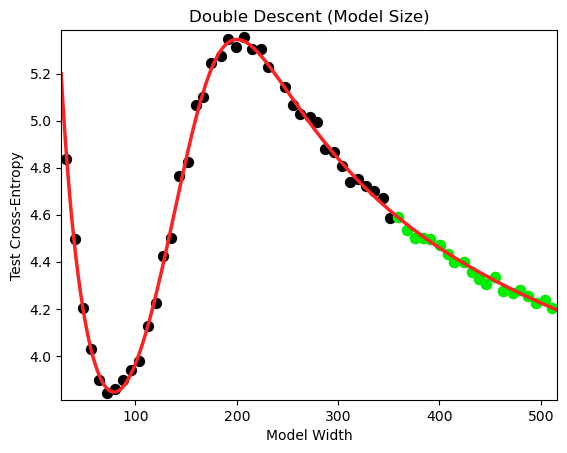
\includegraphics[width=0.48\textwidth]{figures/double_descent/double_descent__model_size.png}
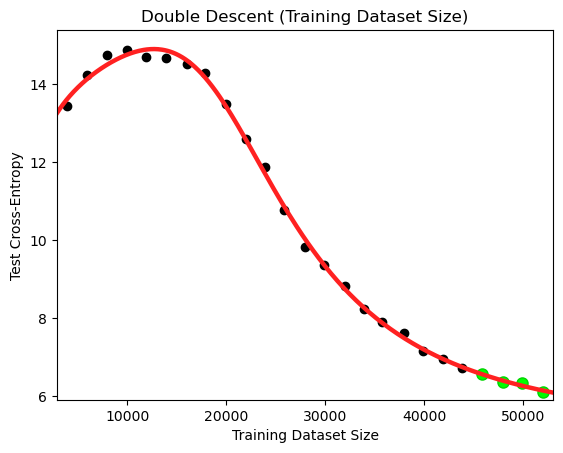
\includegraphics[width=0.48\textwidth]{figures/double_descent/double_descent__dataset_size_1.png}

    \caption{
    Fit of BNSL to Double Descent. Both plots are of transformers trained to do neural machine translation via minimizing cross-entropy. Experimental data of left figure is obtained from Figure 8 top of \cite{nakkiran2021deep}; ``Model Width" on the x-axis refers to embedding dimension $d_{model}$ of the transformer. Experimental data of right figure is obtained from Figure 11b of \cite{nakkiran2021deep}.
    }
    \label{fig:double_descent}
\end{figure*}
\FloatBarrier

\subsection{Inflection Points}
\label{section:Inflection_Points}
We show that BNSL is capable of modeling and extrapolating the scaling behavior of tasks that have an inflection point on a linear-linear plot such as the task of arithmetic (4 digit addition). Other functional forms are mathematically incapable of expressing inflection points on a linear-linear plot (as shown in Section 3) and as a result are mathematically incapable of expressing and modeling inflection points (on a linear-linear plot) that are present in the scaling behaviour of 4 digit addition. In Figure \ref{fig:arithmetic} left, we show that BNSL expresses and accurately models the inflection point present in the scaling behaviour of 4 digit addition and as a result accurately extrapolates the scaling behaviour of 4 digit addition.

\FloatBarrier
\begin{figure*}[htbp]
    \centering


%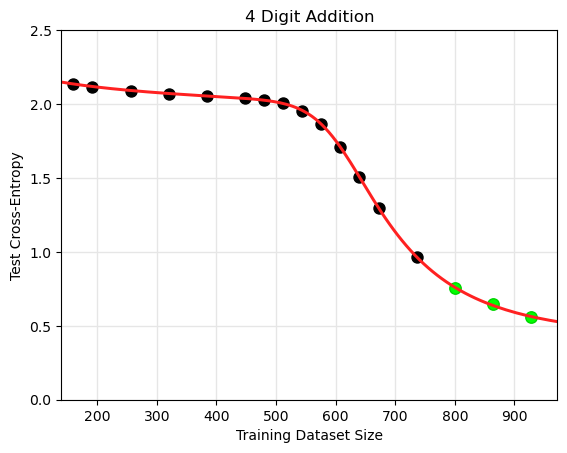
\includegraphics[width=0.48\textwidth]{figures/arithmetic/4_digit_addition__dataset_size.png}
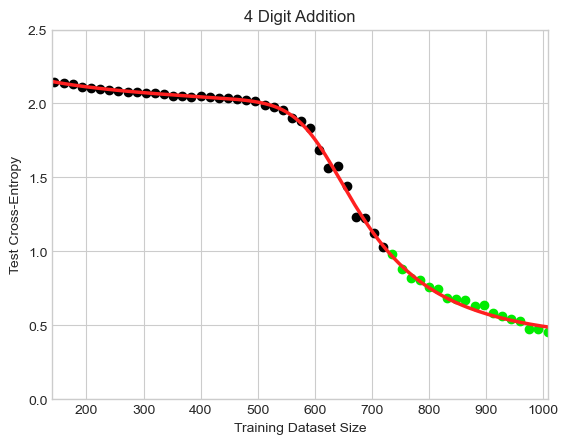
\includegraphics[width=0.48\textwidth]{figures/arithmetic/4_digit_addition__dataset_size__very_first_version.png}
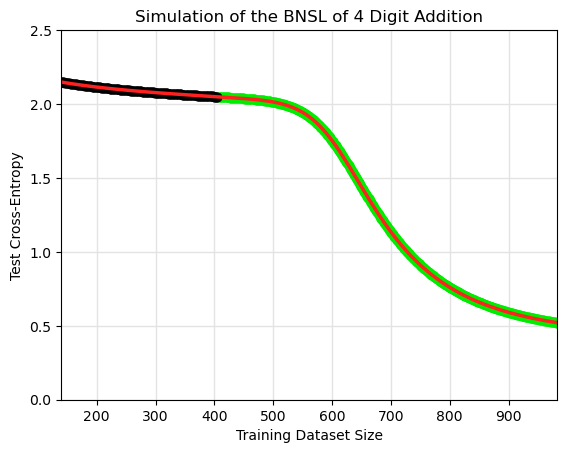
\includegraphics[width=0.48\textwidth]{figures/arithmetic/4_digit_addition__dataset_size__very_first_version__simulation_limit.png}

    \caption{
    4 Digit Addition. Note that these plots are linear-linear. Each point in the left plot is the mean of greater than 100 seeds at that dataset size. In the left plot, each point is gathered from a model trained to do the task of 4 digit addition. In the right plot, each point is gathered from a noiseless simulation of the BNSL of the task of 4 digit addition.
    }
    \label{fig:arithmetic}
\end{figure*}
\FloatBarrier

\subsection{The Limit of the Predictability of Scaling Behavior}
\label{section:limit_of_agi_superforecasting}
We use BNSL to glean insights about the limit of the predictability of scaling behavior. Recent papers \citep{ganguli2022predictability, wei2022emergent} have advertised many task as having ``unpredictable" scaling behavior, the most famous of which being the task of arithmetic. In the previous section and in Figure \ref{fig:arithmetic} left, we successfully predicted (i.e. extrapolated) the scaling behavior of 4 digit addition (arithmetic). However, we are only able to accurately extrapolate the scaling behaviour if given some points from training runs with a training dataset size of at least 720, and the break in which the scaling behaviour of 4 digit addition transitions from one power law to another steeper power law happens at around training dataset size of 415. Ideally, one would like be able to extrapolate the entire scaling behavior by fitting only points from before the break. In Figure \ref{fig:arithmetic} right, we use a noiseless simulation of the BNSL of 4 digit addition to show what would happen if one had infinitely many training runs / seeds to average out all the noisy deviation between runs such that one could recover (i.e. learn via a curve-fitting library such as SciPy \cite{virtanen2020scipy}) the learned constant of the BNSL as well as possible. When using this noiseless simulation, we find that we are only able to accurately extrapolate the scaling behaviour if given some points from training runs with a training dataset size of at least 415, which is very close to the break. This implies that very near to the break there is limit as to how small the supremum of the x-axis of the points used for fitting can be if one wants to perfectly extrapolate the scaling behavior, even if one has infinitely many seeds / training runs.

\subsection{Reinforcement Learning}

TODO: Does RL just go in the appendix because we don't have enough points to get good extrapolations for RL?

\FloatBarrier
\begin{figure*}[htbp]
    \centering


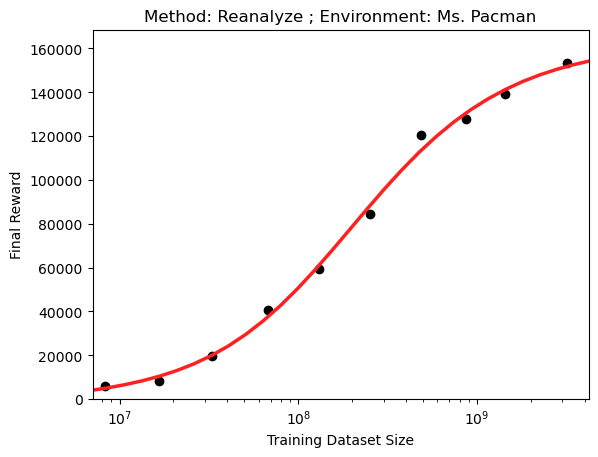
\includegraphics[width=0.48\textwidth]{figures/rl/reanalyze/reanalyze__ms_pacman_dataset_size__fit.png}


    \caption{
    Fit of BNSL to Figure 1 of \cite{schrittwieser2021online}.
    }
    \label{fig:rl_scaling}
\end{figure*}
\FloatBarrier

%\subsection{BIG Bench Emergent}
%Probably will just finish it for rebuttals
%\vspace{-4.9mm}
\section{Empirical Results: Fits and Extrapolations of Functional Forms}
\vspace{-4.25mm}
\label{section:functional_form_fits}

We now show the fits \& extrapolations of various functional forms. \textbf{In all plots here, onward, \& in the appendix, black points are points used for fitting a functional form, \textcolor{Green3}{green} (\textcolor{gray}{gray} if color blind) points are held-out points used for evaluating extrapolation of functional form fit to the black points, \& a \textcolor{red}{red} line is BNSL that has been fit to black points. 100\% of the plots in this paper here \& onward \& in the appendix contain \textcolor{Green3}{green} point(s) for evaluating extrapolation.} See Section \ref{section:BNSL_fit_details} for more details on fitting BNSL \& \textbf{determining the number of breaks}.

\vspace{-1.95mm}

\textbf{Except when stated otherwise}, each plot contains the region(s) surrounding (or neighboring) a single break of a BNSL fit to black points that are smaller (along the x-axis) than the green points.

\vspace{-1.95mm}

\iffalse
\todo[inline]{TODO: remove this list once you fix math proofs; it is redundant}

In the tables and elsewhere, 
\begin{itemize}
    \item M1 refers to functional form $y = ax^b$
    \item M2 refers to functional form $y = ax^b +c$
    \item M3 refers to functional form $y = a(x^{-1} + d)^{-b} + c$
    \item M4 refers to functional form $(y - \epsilon_{\infty}) / ((\epsilon_{0} - y)^a) = bx^c$
\end{itemize}
\fi

All the extrapolation evaluations reported in the tables are reported in terms of root mean squared log error (RMSLE) ± root standard log error. See Appendix \ref{section:definition_of_Root_Mean_Squared_Log_Error} for definition of RMSLE and Appendix \ref{section:definition_of_Root_Standard_Log_Error} for definition of root standard log error.

\vspace{-0.4mm}

%Unless stated otherwise, the BNSL we fit only has one break.
%Except when stated otherwise, each plot contains a single break of the BNSL fit to all the points that are not the green points.

% \begin{center}

%\vspace{-0.1mm}
%\vspace{-1.1mm}
\begin{table}[hbt!]
    \centering
    \begin{tabular}{ |cH|c|c|c|c|c| } 
\hline
Domain & \hspace{.9cm}Task & M1 $\uparrow$ & M2 $\uparrow$ & M3 $\uparrow$ & M4 $\uparrow$ & BNSL $\uparrow$ \\
 \hline
 %IC & Birds 200 & 0 & 0 & 0 & 5.56 & \highlight{94.44}\\ 
 %IC & Caltech101 & 0 & 0 & 5.56 & 5.56 & \highlight{88.89}\\ 
 %IC & CIFAR-100 & 0 & 5.56 & 5.56 & 5.56 & \highlight{83.33}\\
 %IC & ImageNet & 0 & 0 & 11.11 & 0 & \highlight{88.89}\\
 
 %version where Ibrahim had error %Downstream Image Classification & All & 0\% & 1.39\% & 5.56\% & 4.17\% & \bfseries 88.89\%\\
 %Downstream Image Classification & All & 0\% & 1.39\% & 5.56\% & 1.39\% & \bfseries 91.67\%\\
 %Downstream Image Classification & All & 2.78\% & 5.56\% & 13.89\% & 13.89\% & \bfseries 63.89\%\\
%Downstream Image Classification & All & 2.78\% & 4.17\% & 9.72\% & 8.33\% & \bfseries 75.00\%\\
Downstream Image Classification & All & 2.78\% & 4.17\% & 9.72\% & 13.89\% & \bfseries 69.44\%\\
 %version where Ibrahim had error %Language & All & 5\% & 10\% & 15\% & 25\% & \bfseries 45\%\\
 %Language & All & 5\% & 10\% & 15\% & 5\% & \bfseries 65\%\\
 %Language & All & 10\% & 10\% & 25\% & 20\% & \bfseries 35\%\\
 %Language & All & 10\% & 10\% & 25\% & 0\% & \bfseries 55\%\\
 %Language & All & 10\% & 5\% & 25\% & 0\% & \bfseries 60\%\\
 %Language & All & 10\% & 5\% & 20\% & 0\% & \bfseries 65\%\\
 %Language & All & 10\% & 5\% & 15\% & 0\% & \bfseries 70\%\\
 %Language & All & 10\% & 5\% & 10\% & 0\% & \bfseries 75\%\\
 Language (Downstream and Upstream) & All & 10\% & 5\% & 10\% & 0\% & \bfseries 75\%\\
 \hline
\end{tabular}
\vspace{-2.1mm}
    \caption{
    Percentage of tasks by domain where each functional form is the best for extrapolation of scaling behavior. Numbers for M1, M2, M3, and M4 were obtained via correspondence with authors of \cite{Alabdulmohsi2022revisiting}. See Sections \ref{section:scaling_benchmark__vision} and \ref{section:scaling_benchmark__language} for more details.
    }
    \label{table:scaling_laws_benchmark_dataset__summary}
\end{table}
% \end{center}

%\vspace{-2.0mm}
\FloatBarrier
\vspace{-3.6mm}
\subsection{Vision}
\vspace{-3.9mm}
\label{section:scaling_benchmark__vision}

% (TODO: this sentence is repeated in language section)

Using the scaling laws benchmark of \cite{Alabdulmohsi2022revisiting}, we evaluate how well various functional forms extrapolate performance on downstream vision tasks as upstream training dataset size increases. In this large-scale vision subset of the benchmark, the tasks that are evaluated are error rate on each of various few-shot downstream image classification (IC) tasks; the downstream tasks are: Birds 200 \citep{welinder2010caltech}, Caltech101 \citep{fei2004learning}, CIFAR-100 \citep{krizhevsky2009learning}, and ImageNet \citep{deng2009imagenet}. The following architectures of various sizes are pretrained on subsets of JFT-300M \citep{sun2017revisiting}: big-transfer residual neural networks (BiT) \citep{kolesnikov2020big}, MLP mixers (MiX) \citep{tolstikhin2021mlp}, and vision transformers (ViT) \citep{dosovitskiy2020image}. As can be seen in Tables  \ref{table:scaling_laws_benchmark_dataset__summary} and \ref{table:scaling_laws_benchmark_dataset__Vision}, BNSL yields extrapolations with the lowest RMSLE (Root Mean Squared Logarithmic Error) for 69.44\% of tasks of any of the functional forms, while the next best functional form performs the best on only 13.89\% of the tasks.

\iffalse

\todo[inline]{TODO: add diffusion scaling from openai paper or that image reconstruction scaling iclr paper}

\todo[inline]{TODO: maybe try to fit BNSL to relationship between upstream and downstream}

\todo[inline]{TODO: maybe try to fit BNSL to "beyond neural scaling laws" paper}

\fi

%\todo[inline]{TODO: Use multiple breaks to improve extrapolation on Caltech and others; first just try removing early points as easy ablation to know whether multiple breaks will help}

\vspace{-2.0mm}

To view plots of BNSL on each of these tasks, see figures
\ref{fig:scaling_laws_benchmark_dataset__birds},
\ref{fig:scaling_laws_benchmark_dataset__cifar_100},
\ref{fig:scaling_laws_benchmark_dataset__caltech},
\ref{fig:scaling_laws_benchmark_dataset__ImageNet} in Appendix \ref{section:Plots_of_BNSL_Extrapolations}. To view plots of M1, M2, M3, M4 on each of these tasks, see Appendix A.4 of \cite{Alabdulmohsi2022revisiting}.

\vspace{-0.7mm}

In Section \ref{section:vision_tasks__compute_optimal}, we additionally show that BNSL yields accurate extrapolations of performance on large-scale downstream vision tasks when amount of compute used for (pre-)training is on the x-axis and compute is scaled in the manner that is Pareto optimal with respect to the performance evaluation metric on the y-axis (downstream accuracy in this case).

\vspace{-2.2mm}

In Section \ref{section:diffusion}, we additionally show that BNSL yields accurate extrapolations of the scaling behavior of diffusion generative models of images when amount of compute used for (pre-)training is on the x-axis and compute is scaled in the manner that is Pareto optimal with respect to the performance evaluation metric on the y-axis (NLL and FID score in this case).

\vspace{-2.2mm}

In Section \ref{section:video}, we additionally show that BNSL yields accurate extrapolations of the scaling behavior of generative models of video.

\vspace{-2.2mm}

In Section \ref{section:robot}, we show that BNSL yields accurate extrapolations of robotics scaling behavior (out-of-distribution (OOD) generalization and in-distribution generalization).

\vspace{-2.2mm}

%In Section \ref{section:continual}, BNSL yields accurate extrapolations of continual learning scaling behavior.

In Section \ref{section:continual}, BNSL accurately extrapolates the scaling behavior of continual learning.

\vspace{-2.2mm}

In Section \ref{section:adversarial_robustness}, BNSL accurately extrapolates the scaling behavior of adversarial robustness.

\vspace{-2.2mm}

In Section \ref{section:fairness}, BNSL accurately extrapolates the scaling behavior of fairness (and also ensembles).

\vspace{-2.2mm}

In Section \ref{section:extrapolate_contrastive}, we show that BNSL accurately extrapolates the scaling behavior of the downstream performance of multimodal contrastive learning (i.e. non-generative unsupervised learning).

\vspace{-2.2mm}

In Section \ref{section:data_prune}, we additionally show that BNSL yields accurate extrapolations of the scaling behavior when data is pruned Pareto optimally (such that each point along the x-axis uses the subset of the dataset that yields the best performance (y-axis value) for that dataset size (x-axis value)).

\vspace{-2.2mm}

In Section \ref{section:downstream_from_upstream}, we additionally show that BNSL yields accurate extrapolations when upstream performance is on the x-axis and downstream performance is on the y-axis.

\vspace{-2.2mm}

In Section \ref{section:extrapolate_oom} (and Figure \ref{fig:extrapolate_oom_main_paper}), we additionally show that BNSL accurately extrapolates to scales that are an \textbf{order of magnitude} larger than the maximum (along the x-axis) of the points used for fitting.

%\vspace{-9.8mm}

\iffalse

\begin{wraptable}{r}{9}
\tiny
% \fontsize{8}{8}\selectfont
% \setlength\tabcolsep{3.1pt} 
\begin{tabular}
{p{.205\textwidth}p{.111\textwidth}p{.099\textwidth}p{.099\textwidth}p{.099\textwidth}p{.099\textwidth}p{.099\textwidth}}
%\begin{tabular}{llllrrrrrrrrrrrrl}
\hspace{.9cm}Task & Model & M1 $\downarrow$ & M2 $\downarrow$ & M3 $\downarrow$ & M4 $\downarrow$ & BNSL $\downarrow$ \\
\hline
Birds 200 10-shot & BiT/101/3 & 9.13e-2 & 9.13e-2 & 9.13e-2 & 2.49e-2 & \highlight{3.79e-3} \\
Birds 200 10-shot & BiT/50/1 & 6.88e-2 & 6.88e-2 & 5.24e-2 & 2.48e-2 & \highlight{4.96e-3} \\
Birds 200 10-shot & MiX/B/16 & 9.15e-2 & 9.15e-2 & 3.95e-2 & 4.14e-2 & \highlight{9.98e-3} \\
Birds 200 10-shot & MiX/L/16 & 5.51e-2 & 5.51e-2 & 5.51e-2 & 4.59e-2 & \highlight{8.41e-3} \\
Birds 200 10-shot & ViT/B/16 & 6.77e-2 & 6.77e-2 & 3.52e-2 & 1.87e-2 & \highlight{9.81e-3} \\
Birds 200 10-shot & ViT/S/16 & 3.95e-2 & 3.95e-2 & 3.74e-2 & \highlight{9.81e-3} & 1.51e-2 \\
Birds 200 25-shot & BiT/101/3 & 9.41e-2 & 9.41e-2 & 9.41e-2 & 5.09e-2 & \highlight{7.24e-3} \\
Birds 200 25-shot & BiT/50/1 & 1.10e-1 & 7.29e-2 & 1.52e-2 & 1.63e-2 & \highlight{8.00e-3} \\
Birds 200 25-shot & MiX/B/16 & 1.40e-1 & 1.40e-1 & 6.93e-2 & 1.85e-2 & \highlight{5.02e-3} \\
Birds 200 25-shot & MiX/L/16 & 1.12e-1 & 1.12e-1 & 1.12e-1 & 4.88e-2 & \highlight{1.05e-2} \\
Birds 200 25-shot & ViT/B/16 & 9.02e-2 & 9.02e-2 & 3.75e-2 & 1.52e-2 & \highlight{5.87e-3} \\
Birds 200 25-shot & ViT/S/16 & 5.06e-2 & 5.06e-2 & 4.96e-2 & 3.28e-2 & \highlight{1.21e-2} \\
Birds 200 5-shot & BiT/101/3 & 8.17e-2 & 8.17e-2 & 8.17e-2 & 3.00e-2 & \highlight{6.08e-3} \\
Birds 200 5-shot & BiT/50/1 & 5.44e-2 & 5.44e-2 & 5.44e-2 & 2.63e-2 & \highlight{5.79e-3} \\
Birds 200 5-shot & MiX/B/16 & 8.27e-2 & 8.27e-2 & 5.49e-2 & 1.86e-2 & \highlight{5.74e-3} \\
Birds 200 5-shot & MiX/L/16 & 5.68e-2 & 5.68e-2 & 5.68e-2 & 2.65e-2 & \highlight{5.06e-3} \\
Birds 200 5-shot & ViT/B/16 & 3.40e-2 & 3.40e-2 & 3.40e-2 & 1.26e-2 & \highlight{6.32e-3} \\
Birds 200 5-shot & ViT/S/16 & 2.75e-2 & 2.75e-2 & 2.75e-2 & 1.56e-2 & \highlight{6.93e-3} \\
\hline
CIFAR-100 10-shot & BiT/101/3 & 8.57e-2 & 8.57e-2 & 8.25e-2 & 9.28e-2 & \highlight{1.53e-2} \\
CIFAR-100 10-shot & BiT/50/1 & 7.44e-2 & 1.24e-2 & 2.08e-2 & 1.23e-2 & \highlight{9.74e-3} \\
CIFAR-100 10-shot & MiX/B/16 & 8.77e-2 & 8.77e-2 & 2.71e-2 & 2.60e-2 & \highlight{8.61e-3} \\
CIFAR-100 10-shot & MiX/L/16 & 1.05e-1 & 1.05e-1 & 4.85e-2 & 4.76e-2 & \highlight{1.55e-2} \\
CIFAR-100 10-shot & ViT/B/16 & 8.98e-2 & 8.98e-2 & 8.98e-2 & 5.60e-2 & \highlight{1.73e-2} \\
CIFAR-100 10-shot & ViT/S/16 & 6.84e-2 & 2.11e-2 & 3.35e-2 & 2.47e-2 & \highlight{1.15e-2} \\
CIFAR-100 25-shot & BiT/101/3 & 8.77e-2 & 8.77e-2 & 4.44e-2 & 4.29e-2 & \highlight{9.32e-3} \\
CIFAR-100 25-shot & BiT/50/1 & 7.31e-2 & 2.35e-2 & 3.65e-2 & 2.36e-2 & \highlight{2.00e-2} \\
CIFAR-100 25-shot & MiX/B/16 & 1.08e-1 & 4.75e-2 & 2.10e-2 & 2.08e-2 & \highlight{8.15e-3} \\
CIFAR-100 25-shot & MiX/L/16 & 9.79e-2 & 9.79e-2 & 3.67e-2 & 2.79e-2 & \highlight{8.47e-3} \\
CIFAR-100 25-shot & ViT/B/16 & 1.07e-1 & 1.07e-1 & 6.54e-2 & \highlight{4.81e-2} & 1.20e-1 \\
CIFAR-100 25-shot & ViT/S/16 & 8.03e-2 & 2.19e-2 & 3.13e-2 & 2.19e-2 & \highlight{1.34e-2} \\
CIFAR-100 5-shot & BiT/101/3 & 5.94e-2 & 5.94e-2 & 5.94e-2 & 4.57e-2 & \highlight{1.58e-2} \\
CIFAR-100 5-shot & BiT/50/1 & 4.87e-2 & 4.87e-2 & \highlight{1.69e-2} & 4.91e-2 & 1.95e-2 \\
CIFAR-100 5-shot & MiX/B/16 & 7.07e-2 & 7.07e-2 & 2.78e-2 & 2.05e-2 & \highlight{6.77e-3} \\
CIFAR-100 5-shot & MiX/L/16 & 7.06e-2 & 7.06e-2 & 4.17e-2 & 3.14e-2 & \highlight{1.18e-2} \\
CIFAR-100 5-shot & ViT/B/16 & 6.27e-2 & 6.27e-2 & 6.27e-2 & 5.11e-2 & \highlight{1.19e-2} \\
CIFAR-100 5-shot & ViT/S/16 & 6.93e-2 & \highlight{2.84e-2} & 3.88e-2 & 3.09e-2 & 6.40e-2 \\
\hline
Caltech101 10-shot & BiT/101/3 & 3.07e-1 & 3.07e-1 & 1.51e-1 & 3.54e-2 & \highlight{6.42e-3} \\
Caltech101 10-shot & BiT/50/1 & 3.29e-1 & 7.68e-2 & 1.13e-1 & 6.31e-2 & \highlight{5.37e-3} \\
Caltech101 10-shot & MiX/B/16 & 1.35e-1 & 1.35e-1 & 1.35e-1 & 2.11e-1 & \highlight{3.72e-2} \\
Caltech101 10-shot & MiX/L/16 & 1.25e-1 & 1.25e-1 & 1.25e-1 & 1.92e-1 & \highlight{3.73e-2} \\
Caltech101 10-shot & ViT/B/16 & 7.76e-2 & 7.76e-2 & 3.11e-2 & 5.54e-2 & \highlight{1.67e-2} \\
Caltech101 10-shot & ViT/S/16 & 1.95e-1 & 3.41e-2 & \highlight{2.40e-2} & 3.95e-2 & 3.31e-2 \\
Caltech101 25-shot & BiT/101/3 & 1.15e-1 & 1.15e-1 & 1.15e-1 & 5.23e-2 & \highlight{1.13e-2} \\
Caltech101 25-shot & BiT/50/1 & 3.60e-1 & 8.80e-2 & 1.43e-1 & 5.95e-2 & \highlight{2.13e-3} \\
Caltech101 25-shot & MiX/B/16 & 8.28e-2 & 8.28e-2 & 8.28e-2 & 1.74e-1 & \highlight{2.83e-2} \\
Caltech101 25-shot & MiX/L/16 & 9.66e-2 & 9.66e-2 & 9.66e-2 & 1.03e-1 & \highlight{1.98e-2} \\
Caltech101 25-shot & ViT/B/16 & 1.03e-1 & 3.33e-2 & 4.46e-2 & 4.24e-2 & \highlight{6.37e-3} \\
Caltech101 25-shot & ViT/S/16 & 1.77e-1 & 3.79e-2 & 2.80e-2 & \highlight{2.35e-2} & 2.38e-2 \\
Caltech101 5-shot & BiT/101/3 & 2.12e-1 & 2.12e-1 & 2.12e-1 & 8.82e-2 & \highlight{3.17e-3} \\
Caltech101 5-shot & BiT/50/1 & 2.34e-1 & 4.13e-2 & 1.61e-2 & 4.49e-2 & \highlight{1.33e-2} \\
Caltech101 5-shot & MiX/B/16 & 2.43e-1 & 2.43e-1 & 2.35e-1 & 1.23e-1 & \highlight{3.59e-3} \\
Caltech101 5-shot & MiX/L/16 & 1.38e-1 & 1.38e-1 & 1.38e-1 & 3.19e-2 & \highlight{3.19e-2} \\
Caltech101 5-shot & ViT/B/16 & 1.10e-1 & 1.10e-1 & 6.02e-2 & 6.59e-2 & \highlight{2.33e-2} \\
Caltech101 5-shot & ViT/S/16 & 1.90e-1 & 3.82e-2 & 5.04e-2 & 4.06e-2 & \highlight{2.47e-2} \\
\hline
ImageNet 10-shot & BiT/101/3 & 1.27e-1 & 1.27e-1 & 7.36e-2 & 2.13e-2 & \highlight{5.95e-3} \\
ImageNet 10-shot & BiT/50/1 & 9.54e-2 & 9.54e-2 & \highlight{5.75e-3} & 1.77e-2 & 8.93e-3 \\
ImageNet 10-shot & MiX/B/16 & 9.34e-2 & 9.34e-2 & 3.37e-2 & 1.80e-2 & \highlight{5.88e-3} \\
ImageNet 10-shot & MiX/L/16 & 9.83e-2 & 9.83e-2 & 9.83e-2 & 9.48e-3 & \highlight{3.81e-3} \\
ImageNet 10-shot & ViT/B/16 & 4.62e-2 & 4.62e-2 & 4.62e-2 & 3.43e-2 & \highlight{2.85e-3} \\
ImageNet 10-shot & ViT/S/16 & 4.74e-2 & 4.74e-2 & 1.66e-2 & 1.14e-2 & \highlight{1.97e-3} \\
ImageNet 25-shot & BiT/101/3 & 1.42e-1 & 1.42e-1 & 6.67e-2 & 2.18e-2 & \highlight{4.86e-3} \\
ImageNet 25-shot & BiT/50/1 & 1.17e-1 & 1.17e-1 & \highlight{4.06e-3} & 1.70e-2 & 8.14e-3 \\
ImageNet 25-shot & MiX/B/16 & 9.59e-2 & 9.59e-2 & 5.39e-2 & 1.47e-2 & \highlight{2.86e-3} \\
ImageNet 25-shot & MiX/L/16 & 1.03e-1 & 1.03e-1 & 1.03e-1 & 6.09e-3 & \highlight{1.94e-3} \\
ImageNet 25-shot & ViT/B/16 & 5.17e-2 & 5.17e-2 & 5.17e-2 & 3.26e-2 & \highlight{6.91e-3} \\
ImageNet 25-shot & ViT/S/16 & 5.52e-2 & 4.12e-2 & 9.65e-3 & 1.16e-2 & \highlight{3.09e-3} \\
ImageNet 5-shot & BiT/101/3 & 9.24e-2 & 9.24e-2 & 9.24e-2 & 1.01e-2 & \highlight{2.55e-3} \\
ImageNet 5-shot & BiT/50/1 & 8.95e-2 & 8.95e-2 & 1.53e-2 & 1.03e-2 & \highlight{4.00e-3} \\
ImageNet 5-shot & MiX/B/16 & 9.09e-2 & 9.09e-2 & 3.01e-2 & 1.45e-2 & \highlight{3.57e-3} \\
ImageNet 5-shot & MiX/L/16 & 7.99e-2 & 7.99e-2 & 7.99e-2 & 5.66e-3 & \highlight{1.63e-3} \\
ImageNet 5-shot & ViT/B/16 & 4.11e-2 & 4.11e-2 & 4.11e-2 & 2.88e-2 & \highlight{4.97e-3} \\
ImageNet 5-shot & ViT/S/16 & 4.20e-2 & 4.20e-2 & 2.40e-2 & 1.44e-2 & \highlight{3.00e-3} \\
\end{tabular}
    \caption{
    Extrapolation Results for Vision Tasks. See Section \ref{section:scaling_benchmark__vision} for more details. Numbers for M1, M2, M3, and M4 obtained via correspondence with authors of \cite{Alabdulmohsi2022revisiting}. 
    }
    \label{table:scaling_laws_benchmark_dataset__Vision_old}
\end{wraptable}
\FloatBarrier

\begin{table}[htbp]
\setlength\tabcolsep{2.1pt} 
\begin{adjustwidth}{-2.2cm}{-1cm}
\fontsize{8}{10}\selectfont
% \setlength\tabcolsep{3.1pt} 
\begin{tabular}
{|p{.165\textwidth} c c c c c || p{.165\textwidth} c c c c c |}
%{p{.02\textwidth}p{.165\textwidth}p{.095\textwidth}p{.01\textwidth}p{.01\textwidth}p{.099\textwidth}p{.099\textwidth}p{.099\textwidth}p{.099\textwidth}p{.099\textwidth}}
% {p{.165\textwidth}p{.070\textwidth}p{.070\textwidth}p{.080\textwidth}p{.080\textwidth}p{.080\textwidth}p{.165\textwidth}p{.080\textwidth}p{.080\textwidth}p{.080\textwidth}p{.080\textwidth}p{.080\textwidth}}
%\begin{tabular}{llllrrrrrrrrrrrrl}
%\hline
%\multicolumn{6}{c}{Sum of Extracted Bits}
\hline
\hspace{.9cm}Task & M1 $\downarrow$ & M2 $\downarrow$ & M3 $\downarrow$ & M4 $\downarrow$ & BNSL $\downarrow$ & \hspace{.9cm}Task & M1 $\downarrow$ & M2 $\downarrow$ & M3 $\downarrow$ & M4 $\downarrow$ & BNSL $\downarrow$\\
\hline
Birds 200 10-shot & 9.13e-2 & 9.13e-2 & 9.13e-2 & 2.49e-2 & \highlight{3.79e-3} & CIFAR-100 10-shot & 8.57e-2 & 8.57e-2 & 8.25e-2 & 9.28e-2 & \highlight{1.53e-2} \\
Birds 200 10-shot & 6.88e-2 & 6.88e-2 & 5.24e-2 & 2.48e-2 & \highlight{4.96e-3} & CIFAR-100 10-shot & 7.44e-2 & 1.24e-2 & 2.08e-2 & 1.23e-2 & \highlight{9.74e-3} \\
Birds 200 10-shot & 9.15e-2 & 9.15e-2 & 3.95e-2 & 4.14e-2 & \highlight{9.98e-3} & CIFAR-100 10-shot & 8.77e-2 & 8.77e-2 & 2.71e-2 & 2.60e-2 & \highlight{8.61e-3} \\
Birds 200 10-shot & 5.51e-2 & 5.51e-2 & 5.51e-2 & 4.59e-2 & \highlight{8.41e-3} & CIFAR-100 10-shot & 1.05e-1 & 1.05e-1 & 4.85e-2 & 4.76e-2 & \highlight{1.55e-2} \\
Birds 200 10-shot & 6.77e-2 & 6.77e-2 & 3.52e-2 & 1.87e-2 & \highlight{9.81e-3} & CIFAR-100 10-shot & 8.98e-2 & 8.98e-2 & 8.98e-2 & 5.60e-2 & \highlight{1.73e-2} \\
Birds 200 10-shot & 3.95e-2 & 3.95e-2 & 3.74e-2 & \highlight{9.81e-3} & 1.51e-2 & CIFAR-100 10-shot & 6.84e-2 & 2.11e-2 & 3.35e-2 & 2.47e-2 & \highlight{1.15e-2} \\
Birds 200 25-shot & 9.41e-2 & 9.41e-2 & 9.41e-2 & 5.09e-2 & \highlight{7.24e-3} & CIFAR-100 25-shot & 8.77e-2 & 8.77e-2 & 4.44e-2 & 4.29e-2 & \highlight{9.32e-3} \\
Birds 200 25-shot & 1.10e-1 & 7.29e-2 & 1.52e-2 & 1.63e-2 & \highlight{8.00e-3} & CIFAR-100 25-shot & 7.31e-2 & 2.35e-2 & 3.65e-2 & 2.36e-2 & \highlight{2.00e-2} \\
Birds 200 25-shot & 1.40e-1 & 1.40e-1 & 6.93e-2 & 1.85e-2 & \highlight{5.02e-3} & CIFAR-100 25-shot & 1.08e-1 & 4.75e-2 & 2.10e-2 & 2.08e-2 & \highlight{8.15e-3} \\
Birds 200 25-shot & 1.12e-1 & 1.12e-1 & 1.12e-1 & 4.88e-2 & \highlight{1.05e-2} & CIFAR-100 25-shot & 9.79e-2 & 9.79e-2 & 3.67e-2 & 2.79e-2 & \highlight{8.47e-3} \\
Birds 200 25-shot & 9.02e-2 & 9.02e-2 & 3.75e-2 & 1.52e-2 & \highlight{5.87e-3} & CIFAR-100 25-shot & 1.07e-1 & 1.07e-1 & 6.54e-2 & \highlight{4.81e-2} & 1.20e-1 \\
Birds 200 25-shot & 5.06e-2 & 5.06e-2 & 4.96e-2 & 3.28e-2 & \highlight{1.21e-2} & CIFAR-100 25-shot & 8.03e-2 & 2.19e-2 & 3.13e-2 & 2.19e-2 & \highlight{1.34e-2} \\
Birds 200 5-shot & 8.17e-2 & 8.17e-2 & 8.17e-2 & 3.00e-2 & \highlight{6.08e-3} & CIFAR-100 5-shot & 5.94e-2 & 5.94e-2 & 5.94e-2 & 4.57e-2 & \highlight{1.58e-2} \\
Birds 200 5-shot & 5.44e-2 & 5.44e-2 & 5.44e-2 & 2.63e-2 & \highlight{5.79e-3} & CIFAR-100 5-shot & 4.87e-2 & 4.87e-2 & \highlight{1.69e-2} & 4.91e-2 & 1.95e-2 \\
Birds 200 5-shot & 8.27e-2 & 8.27e-2 & 5.49e-2 & 1.86e-2 & \highlight{5.74e-3} & CIFAR-100 5-shot & 7.07e-2 & 7.07e-2 & 2.78e-2 & 2.05e-2 & \highlight{6.77e-3} \\
Birds 200 5-shot & 5.68e-2 & 5.68e-2 & 5.68e-2 & 2.65e-2 & \highlight{5.06e-3} & CIFAR-100 5-shot & 7.06e-2 & 7.06e-2 & 4.17e-2 & 3.14e-2 & \highlight{1.18e-2} \\
Birds 200 5-shot & 3.40e-2 & 3.40e-2 & 3.40e-2 & 1.26e-2 & \highlight{6.32e-3} & CIFAR-100 5-shot & 6.27e-2 & 6.27e-2 & 6.27e-2 & 5.11e-2 & \highlight{1.19e-2} \\
Birds 200 5-shot & 2.75e-2 & 2.75e-2 & 2.75e-2 & 1.56e-2 & \highlight{6.93e-3} & CIFAR-100 5-shot & 6.93e-2 & \highlight{2.84e-2} & 3.88e-2 & 3.09e-2 & 6.40e-2 \\
\hline
\hline
Caltech101 10-shot & 3.07e-1 & 3.07e-1 & 1.51e-1 & 3.54e-2 & \highlight{6.42e-3} & ImageNet 10-shot & 1.27e-1 & 1.27e-1 & 7.36e-2 & 2.13e-2 & \highlight{5.95e-3} \\
Caltech101 10-shot & 3.29e-1 & 7.68e-2 & 1.13e-1 & 6.31e-2 & \highlight{5.37e-3} & ImageNet 10-shot & 9.54e-2 & 9.54e-2 & \highlight{5.75e-3} & 1.77e-2 & 8.93e-3 \\
Caltech101 10-shot & 1.35e-1 & 1.35e-1 & 1.35e-1 & 2.11e-1 & \highlight{3.72e-2} & ImageNet 10-shot & 9.34e-2 & 9.34e-2 & 3.37e-2 & 1.80e-2 & \highlight{5.88e-3} \\
Caltech101 10-shot & 1.25e-1 & 1.25e-1 & 1.25e-1 & 1.92e-1 & \highlight{3.73e-2} & ImageNet 10-shot & 9.83e-2 & 9.83e-2 & 9.83e-2 & 9.48e-3 & \highlight{3.81e-3} \\
Caltech101 10-shot & 7.76e-2 & 7.76e-2 & 3.11e-2 & 5.54e-2 & \highlight{1.67e-2} & ImageNet 10-shot & 4.62e-2 & 4.62e-2 & 4.62e-2 & 3.43e-2 & \highlight{2.85e-3} \\
Caltech101 10-shot & 1.95e-1 & 3.41e-2 & \highlight{2.40e-2} & 3.95e-2 & 3.31e-2 & ImageNet 10-shot & 4.74e-2 & 4.74e-2 & 1.66e-2 & 1.14e-2 & \highlight{1.97e-3} \\
Caltech101 25-shot & 1.15e-1 & 1.15e-1 & 1.15e-1 & 5.23e-2 & \highlight{1.13e-2} & ImageNet 25-shot & 1.42e-1 & 1.42e-1 & 6.67e-2 & 2.18e-2 & \highlight{4.86e-3} \\
Caltech101 25-shot & 3.60e-1 & 8.80e-2 & 1.43e-1 & 5.95e-2 & \highlight{2.13e-3} & ImageNet 25-shot & 1.17e-1 & 1.17e-1 & \highlight{4.06e-3} & 1.70e-2 & 8.14e-3 \\
Caltech101 25-shot & 8.28e-2 & 8.28e-2 & 8.28e-2 & 1.74e-1 & \highlight{2.83e-2} & ImageNet 25-shot & 9.59e-2 & 9.59e-2 & 5.39e-2 & 1.47e-2 & \highlight{2.86e-3} \\
Caltech101 25-shot & 9.66e-2 & 9.66e-2 & 9.66e-2 & 1.03e-1 & \highlight{1.98e-2} & ImageNet 25-shot & 1.03e-1 & 1.03e-1 & 1.03e-1 & 6.09e-3 & \highlight{1.94e-3} \\
Caltech101 25-shot & 1.03e-1 & 3.33e-2 & 4.46e-2 & 4.24e-2 & \highlight{6.37e-3} & ImageNet 25-shot & 5.17e-2 & 5.17e-2 & 5.17e-2 & 3.26e-2 & \highlight{6.91e-3} \\
Caltech101 25-shot & 1.77e-1 & 3.79e-2 & 2.80e-2 & \highlight{2.35e-2} & 2.38e-2 & ImageNet 25-shot & 5.52e-2 & 4.12e-2 & 9.65e-3 & 1.16e-2 & \highlight{3.09e-3} \\
Caltech101 5-shot & 2.12e-1 & 2.12e-1 & 2.12e-1 & 8.82e-2 & \highlight{3.17e-3} & ImageNet 5-shot & 9.24e-2 & 9.24e-2 & 9.24e-2 & 1.01e-2 & \highlight{2.55e-3} \\
Caltech101 5-shot & 2.34e-1 & 4.13e-2 & 1.61e-2 & 4.49e-2 & \highlight{1.33e-2} & ImageNet 5-shot & 8.95e-2 & 8.95e-2 & 1.53e-2 & 1.03e-2 & \highlight{4.00e-3} \\
Caltech101 5-shot & 2.43e-1 & 2.43e-1 & 2.35e-1 & 1.23e-1 & \highlight{3.59e-3} & ImageNet 5-shot & 9.09e-2 & 9.09e-2 & 3.01e-2 & 1.45e-2 & \highlight{3.57e-3} \\
Caltech101 5-shot & 1.38e-1 & 1.38e-1 & 1.38e-1 & 3.19e-2 & \highlight{3.19e-2} & ImageNet 5-shot & 7.99e-2 & 7.99e-2 & 7.99e-2 & 5.66e-3 & \highlight{1.63e-3} \\
Caltech101 5-shot & 1.10e-1 & 1.10e-1 & 6.02e-2 & 6.59e-2 & \highlight{2.33e-2} & ImageNet 5-shot & 4.11e-2 & 4.11e-2 & 4.11e-2 & 2.88e-2 & \highlight{4.97e-3} \\
Caltech101 5-shot & 1.90e-1 & 3.82e-2 & 5.04e-2 & 4.06e-2 & \highlight{2.47e-2} & ImageNet 5-shot & 4.20e-2 & 4.20e-2 & 2.40e-2 & 1.44e-2 & \highlight{3.00e-3} \\
\hline
\end{tabular}
    \caption{
    Extrapolation Results for Vision Tasks. See Section \ref{section:scaling_benchmark__vision} for more details. Numbers for M1, M2, M3, and M4 obtained via correspondence with authors of \cite{Alabdulmohsi2022revisiting}. 
    }
    \label{table:scaling_laws_benchmark_dataset__Vision_old}
\end{adjustwidth}
\end{table}
\FloatBarrier

\fi

%version in which Ibrahim had error
\iffalse

%\small is default
%\tiny, \scriptsize, \footnotesize, \small, \normalsize, \large, \Large, \LARGE, \huge, and \Huge
%\begin{table}[hbt!]
\begin{table}[]
%\tiny
%\footnotesize
\scriptsize
\setlength\tabcolsep{3.1pt} 
\setlength{\extrarowheight}{0.4pt}
\begin{tabular}
%{p{.021\textwidth}p{.165\textwidth}p{.111\textwidth}p{.028\textwidth}p{.022\textwidth}p{.099\textwidth}p{.099\textwidth}p{.099\textwidth}p{.099\textwidth}p{.099\textwidth}}
%{Hp{.21\textwidth}p{.111\textwidth}HHp{.165\textwidth}p{.165\textwidth}p{.165\textwidth}p{.165\textwidth}p{.165\textwidth}}
%{Hp{.15\textwidth}p{.08\textwidth}HHp{.13\textwidth}p{.13\textwidth}p{.13\textwidth}p{.13\textwidth}p{.13\textwidth}}
{Hp{.14\textwidth}p{.08\textwidth}HH|p{.13\textwidth}|p{.13\textwidth}|p{.13\textwidth}|p{.13\textwidth}|p{.13\textwidth}}
%\begin{tabular}{llllrrrrrrrrrrrrl}
Domain & Task & Model & Train Points & Test Points & M1 $\downarrow$ & M2 $\downarrow$ & M3 $\downarrow$ & M4 $\downarrow$ & BNSL $\downarrow$ \\
\hline
IC & Birds 200 10-shot & BiT/101/3 & 57 & 107 & 9.13e-2 ± 2.8e-3 & 9.13e-2 ± 2.8e-3 & 9.13e-2 ± 2.8e-3 & 2.49e-2 ± 1.2e-3 & \bfseries 3.79e-3 ± 1.1e-3 \\
IC & Birds 200 10-shot & BiT/50/1 & 70 & 469 & 6.88e-2 ± 7.5e-4 & 6.88e-2 ± 7.5e-4 & 5.24e-2 ± 6.2e-4 & 2.48e-2 ± 5.1e-4 & \bfseries 4.96e-3 ± 3.9e-4 \\
IC & Birds 200 10-shot & MiX/B/16 & 69 & 383 & 9.15e-2 ± 1.1e-3 & 9.15e-2 ± 1.1e-3 & 3.95e-2 ± 7.0e-4 & 4.14e-2 ± 7.8e-4 & \bfseries 9.98e-3 ± 7.0e-4 \\
IC & Birds 200 10-shot & MiX/L/16 & 63 & 211 & 5.51e-2 ± 1.4e-3 & 5.51e-2 ± 1.4e-3 & 5.51e-2 ± 1.4e-3 & 4.59e-2 ± 1.6e-3 & \bfseries 8.41e-3 ± 1.3e-3 \\
IC & Birds 200 10-shot & ViT/B/16 & 65 & 316 & 6.77e-2 ± 1.1e-3 & 6.77e-2 ± 1.1e-3 & 3.52e-2 ± 8.1e-4 & 1.87e-2 ± 7.2e-4 & \bfseries 9.81e-3 ± 8.1e-4 \\
IC & Birds 200 10-shot & ViT/S/16 & 54 & 133 & 3.95e-2 ± 1.2e-3 & 3.95e-2 ± 1.2e-3 & 3.74e-2 ± 1.1e-3 & \bfseries 9.81e-3 ± 5.4e-4 & 1.51e-2 ± 8.4e-4 \\
IC & Birds 200 25-shot & BiT/101/3 & 53 & 78 & 9.41e-2 ± 3.2e-3 & 9.41e-2 ± 3.2e-3 & 9.41e-2 ± 3.2e-3 & 5.09e-2 ± 1.8e-3 & \bfseries 7.24e-3 ± 1.6e-3 \\
IC & Birds 200 25-shot & BiT/50/1 & 69 & 452 & 1.10e-1 ± 1.0e-3 & 7.29e-2 ± 8.0e-4 & 1.52e-2 ± 4.9e-4 & 1.63e-2 ± 5.1e-4 & \bfseries 8.00e-3 ± 6.1e-4 \\
IC & Birds 200 25-shot & MiX/B/16 & 67 & 293 & 1.40e-1 ± 1.9e-3 & 1.40e-1 ± 1.9e-3 & 6.93e-2 ± 1.2e-3 & 1.85e-2 ± 6.3e-4 & \bfseries 5.02e-3 ± 6.2e-4 \\
IC & Birds 200 25-shot & MiX/L/16 & 63 & 196 & 1.12e-1 ± 2.0e-3 & 1.12e-1 ± 2.0e-3 & 1.12e-1 ± 2.0e-3 & 4.88e-2 ± 1.8e-3 & \bfseries 1.05e-2 ± 1.7e-3 \\
IC & Birds 200 25-shot & ViT/B/16 & 64 & 271 & 9.02e-2 ± 1.6e-3 & 9.02e-2 ± 1.6e-3 & 3.75e-2 ± 1.0e-3 & 1.52e-2 ± 5.8e-4 & \bfseries 5.87e-3 ± 6.1e-4 \\
IC & Birds 200 25-shot & ViT/S/16 & 51 & 100 & 5.06e-2 ± 1.4e-3 & 5.06e-2 ± 1.4e-3 & 4.96e-2 ± 1.4e-3 & 3.28e-2 ± 1.1e-3 & \bfseries 1.21e-2 ± 8.5e-4 \\
IC & Birds 200 5-shot & BiT/101/3 & 62 & 180 & 8.17e-2 ± 2.0e-3 & 8.17e-2 ± 2.0e-3 & 8.17e-2 ± 2.0e-3 & 3.00e-2 ± 1.2e-3 & \bfseries 6.08e-3 ± 1.1e-3 \\
IC & Birds 200 5-shot & BiT/50/1 & 71 & 517 & 5.44e-2 ± 5.6e-4 & 5.44e-2 ± 5.6e-4 & 5.44e-2 ± 5.6e-4 & 2.63e-2 ± 5.4e-4 & \bfseries 5.79e-3 ± 3.7e-4 \\
IC & Birds 200 5-shot & MiX/B/16 & 71 & 494 & 8.27e-2 ± 1.0e-3 & 8.27e-2 ± 1.0e-3 & 5.49e-2 ± 7.8e-4 & 1.86e-2 ± 5.0e-4 & \bfseries 5.74e-3 ± 4.7e-4 \\
IC & Birds 200 5-shot & MiX/L/16 & 67 & 326 & 5.68e-2 ± 1.4e-3 & 5.68e-2 ± 1.4e-3 & 5.68e-2 ± 1.4e-3 & 2.65e-2 ± 9.0e-4 & \bfseries 5.06e-3 ± 6.4e-4 \\
IC & Birds 200 5-shot & ViT/B/16 & 65 & 284 & 3.40e-2 ± 8.9e-4 & 3.40e-2 ± 8.9e-4 & 3.40e-2 ± 8.9e-4 & 1.26e-2 ± 5.3e-4 & \bfseries 6.32e-3 ± 5.8e-4 \\
IC & Birds 200 5-shot & ViT/S/16 & 57 & 150 & 2.75e-2 ± 7.9e-4 & 2.75e-2 ± 7.9e-4 & 2.75e-2 ± 7.9e-4 & 1.56e-2 ± 5.9e-4 & \bfseries 6.93e-3 ± 4.8e-4 \\
IC & CIFAR-100 10-shot & BiT/101/3 & 47 & 60 & 8.57e-2 ± 3.8e-3 & 8.57e-2 ± 3.8e-3 & 8.25e-2 ± 3.7e-3 & 9.28e-2 ± 3.9e-3 & \bfseries 1.53e-2 ± 2.9e-3 \\
IC & CIFAR-100 10-shot & BiT/50/1 & 62 & 192 & 7.44e-2 ± 1.5e-3 & 1.24e-2 ± 5.8e-4 & 2.08e-2 ± 7.2e-4 & 1.23e-2 ± 5.7e-4 & \bfseries 9.74e-3 ± 7.1e-4 \\
IC & CIFAR-100 10-shot & MiX/B/16 & 65 & 248 & 8.77e-2 ± 1.9e-3 & 8.77e-2 ± 1.9e-3 & 2.71e-2 ± 1.2e-3 & 2.60e-2 ± 1.2e-3 & \bfseries 8.61e-3 ± 9.5e-4 \\
IC & CIFAR-100 10-shot & MiX/L/16 & 67 & 313 & 1.05e-1 ± 3.1e-3 & 1.05e-1 ± 3.1e-3 & 4.85e-2 ± 2.6e-3 & 4.76e-2 ± 1.7e-3 & \bfseries 1.55e-2 ± 1.6e-3 \\
IC & CIFAR-100 10-shot & ViT/B/16 & 67 & 354 & 8.98e-2 ± 2.0e-3 & 8.98e-2 ± 2.0e-3 & 8.98e-2 ± 2.0e-3 & 5.60e-2 ± 1.8e-3 & \bfseries 1.73e-2 ± 1.8e-3 \\
IC & CIFAR-100 10-shot & ViT/S/16 & 67 & 450 & 6.84e-2 ± 1.1e-3 & 2.11e-2 ± 6.6e-4 & 3.35e-2 ± 8.6e-4 & 2.47e-2 ± 7.4e-4 & \bfseries 1.15e-2 ± 7.5e-4 \\
IC & CIFAR-100 25-shot & BiT/101/3 & 41 & 38 & 8.77e-2 ± 5.6e-3 & 8.77e-2 ± 5.6e-3 & 4.44e-2 ± 3.5e-3 & 4.29e-2 ± 3.4e-3 & \bfseries 9.32e-3 ± 3.0e-3 \\
IC & CIFAR-100 25-shot & BiT/50/1 & 55 & 109 & 7.31e-2 ± 2.0e-3 & 2.35e-2 ± 1.5e-3 & 3.65e-2 ± 1.8e-3 & 2.36e-2 ± 1.5e-3 & \bfseries 2.00e-2 ± 1.8e-3 \\
IC & CIFAR-100 25-shot & MiX/B/16 & 64 & 202 & 1.08e-1 ± 2.3e-3 & 4.75e-2 ± 1.6e-3 & 2.10e-2 ± 9.4e-4 & 2.08e-2 ± 9.3e-4 & \bfseries 8.15e-3 ± 1.1e-3 \\
IC & CIFAR-100 25-shot & MiX/L/16 & 62 & 185 & 9.79e-2 ± 2.2e-3 & 9.79e-2 ± 2.2e-3 & 3.67e-2 ± 1.7e-3 & 2.79e-2 ± 1.3e-3 & \bfseries 8.47e-3 ± 1.6e-3 \\
IC & CIFAR-100 25-shot & ViT/B/16 & 66 & 355 & 1.07e-1 ± 1.9e-3 & 1.07e-1 ± 1.9e-3 & 6.54e-2 ± 1.6e-3 & \bfseries 4.81e-2 ± 1.4e-3 & 1.20e-1 ± 1.4e-3 \\
IC & CIFAR-100 25-shot & ViT/S/16 & 66 & 416 & 8.03e-2 ± 1.2e-3 & 2.19e-2 ± 7.4e-4 & 3.13e-2 ± 8.4e-4 & 2.19e-2 ± 7.0e-4 & \bfseries 1.34e-2 ± 8.5e-4 \\
IC & CIFAR-100 5-shot & BiT/101/3 & 47 & 59 & 5.94e-2 ± 3.2e-3 & 5.94e-2 ± 3.2e-3 & 5.94e-2 ± 3.2e-3 & 4.57e-2 ± 2.8e-3 & \bfseries 1.58e-2 ± 2.6e-3 \\
IC & CIFAR-100 5-shot & BiT/50/1 & 57 & 98 & 4.87e-2 ± 1.3e-3 & 4.87e-2 ± 1.3e-3 & \bfseries 1.69e-2 ± 8.8e-4 & 4.91e-2 ± 1.3e-3 & 1.95e-2 ± 1.0e-3 \\
IC & CIFAR-100 5-shot & MiX/B/16 & 66 & 304 & 7.07e-2 ± 1.2e-3 & 7.07e-2 ± 1.2e-3 & 2.78e-2 ± 8.4e-4 & 2.05e-2 ± 7.4e-4 & \bfseries 6.77e-3 ± 6.3e-4 \\
IC & CIFAR-100 5-shot & MiX/L/16 & 67 & 312 & 7.06e-2 ± 1.6e-3 & 7.06e-2 ± 1.6e-3 & 4.17e-2 ± 1.4e-3 & 3.14e-2 ± 1.1e-3 & \bfseries 1.18e-2 ± 1.3e-3 \\
IC & CIFAR-100 5-shot & ViT/B/16 & 67 & 352 & 6.27e-2 ± 1.6e-3 & 6.27e-2 ± 1.6e-3 & 6.27e-2 ± 1.6e-3 & 5.11e-2 ± 1.4e-3 & \bfseries 1.19e-2 ± 1.2e-3 \\
IC & CIFAR-100 5-shot & ViT/S/16 & 70 & 710 & 6.93e-2 ± 1.2e-3 & \bfseries 2.84e-2 ± 8.2e-4 & 3.88e-2 ± 8.0e-4 & 3.09e-2 ± 7.5e-4 & 6.40e-2 ± 7.7e-4 \\
IC & Caltech101 10-shot & BiT/101/3 & 21 & 14 & 3.07e-1 ± 2.0e-2 & 3.07e-1 ± 2.0e-2 & 1.51e-1 ± 1.3e-2 & 3.54e-2 ± 6.3e-3 & \bfseries 6.42e-3 ± 5.8e-3 \\
IC & Caltech101 10-shot & BiT/50/1 & 33 & 16 & 3.29e-1 ± 1.6e-2 & 7.68e-2 ± 5.0e-3 & 1.13e-1 ± 6.0e-3 & 6.31e-2 ± 4.4e-3 & \bfseries 5.37e-3 ± 2.2e-3 \\
IC & Caltech101 10-shot & MiX/B/16 & 14 & 12 & 1.35e-1 ± 1.4e-2 & 1.35e-1 ± 1.4e-2 & 1.35e-1 ± 1.4e-2 & 2.11e-1 ± 1.7e-2 & \bfseries 3.72e-2 ± 9.7e-3 \\
IC & Caltech101 10-shot & MiX/L/16 & 12 & 11 & 1.25e-1 ± 1.3e-2 & 1.25e-1 ± 1.3e-2 & 1.25e-1 ± 1.3e-2 & 1.92e-1 ± 1.6e-2 & \bfseries 3.73e-2 ± 1.5e-2 \\
IC & Caltech101 10-shot & ViT/B/16 & 34 & 33 & 7.76e-2 ± 4.3e-3 & 7.76e-2 ± 4.3e-3 & 3.11e-2 ± 3.0e-3 & 5.54e-2 ± 4.3e-3 & \bfseries 1.67e-2 ± 5.4e-3 \\
IC & Caltech101 10-shot & ViT/S/16 & 43 & 55 & 1.95e-1 ± 6.0e-3 & 3.41e-2 ± 2.9e-3 & \bfseries 2.40e-2 ± 2.0e-3 & 3.95e-2 ± 3.1e-3 & 3.31e-2 ± 5.3e-3 \\
IC & Caltech101 25-shot & BiT/101/3 & 10 & 3 & 1.15e-1 ± 6.5e-3 & 1.15e-1 ± 6.5e-3 & 1.15e-1 ± 6.5e-3 & 5.23e-2 ± 2.7e-3 & \bfseries 1.13e-2 ± 8.0e-3 \\
IC & Caltech101 25-shot & BiT/50/1 & 28 & 16 & 3.60e-1 ± 1.9e-2 & 8.80e-2 ± 5.5e-3 & 1.43e-1 ± 7.6e-3 & 5.95e-2 ± 4.1e-3 & \bfseries 2.13e-3 ± 1.6e-3 \\
IC & Caltech101 25-shot & MiX/B/16 & 13 & 11 & 8.28e-2 ± 1.2e-2 & 8.28e-2 ± 1.2e-2 & 8.28e-2 ± 1.2e-2 & 1.74e-1 ± 1.7e-2 & \bfseries 2.83e-2 ± 1.3e-2 \\
IC & Caltech101 25-shot & MiX/L/16 & 12 & 12 & 9.66e-2 ± 1.0e-2 & 9.66e-2 ± 1.0e-2 & 9.66e-2 ± 1.0e-2 & 1.03e-1 ± 9.5e-3 & \bfseries 1.98e-2 ± 1.3e-2 \\
IC & Caltech101 25-shot & ViT/B/16 & 27 & 28 & 1.03e-1 ± 5.6e-3 & 3.33e-2 ± 2.5e-3 & 4.46e-2 ± 3.6e-3 & 4.24e-2 ± 3.6e-3 & \bfseries 6.37e-3 ± 5.4e-3 \\
IC & Caltech101 25-shot & ViT/S/16 & 41 & 54 & 1.77e-1 ± 5.4e-3 & 3.79e-2 ± 3.1e-3 & 2.80e-2 ± 1.8e-3 & \bfseries 2.35e-2 ± 2.3e-3 & 2.38e-2 ± 4.7e-3 \\
IC & Caltech101 5-shot & BiT/101/3 & 16 & 13 & 2.12e-1 ± 1.2e-2 & 2.12e-1 ± 1.2e-2 & 2.12e-1 ± 1.2e-2 & 8.82e-2 ± 5.0e-3 & \bfseries 3.17e-3 ± 4.3e-3 \\
IC & Caltech101 5-shot & BiT/50/1 & 46 & 54 & 2.34e-1 ± 6.1e-3 & 4.13e-2 ± 2.1e-3 & 1.61e-2 ± 1.3e-3 & 4.49e-2 ± 2.1e-3 & \bfseries 1.33e-2 ± 2.2e-3 \\
IC & Caltech101 5-shot & MiX/B/16 & 24 & 19 & 2.43e-1 ± 1.2e-2 & 2.43e-1 ± 1.2e-2 & 2.35e-1 ± 1.1e-2 & 1.23e-1 ± 6.0e-3 & \bfseries 3.59e-3 ± 1.9e-3 \\
IC & Caltech101 5-shot & MiX/L/16 & 14 & 13 & 1.38e-1 ± 9.7e-3 & 1.38e-1 ± 9.7e-3 & 1.38e-1 ± 9.7e-3 & 3.19e-2 ± 2.6e-3 & \bfseries 3.19e-2 ± 1.1e-2 \\
IC & Caltech101 5-shot & ViT/B/16 & 38 & 41 & 1.10e-1 ± 6.3e-3 & 1.10e-1 ± 6.3e-3 & 6.02e-2 ± 4.7e-3 & 6.59e-2 ± 4.7e-3 & \bfseries 2.33e-2 ± 6.0e-3 \\
IC & Caltech101 5-shot & ViT/S/16 & 49 & 82 & 1.90e-1 ± 4.7e-3 & 3.82e-2 ± 2.6e-3 & 5.04e-2 ± 2.9e-3 & 4.06e-2 ± 2.7e-3 & \bfseries 2.47e-2 ± 3.8e-3 \\
IC & ImageNet 10-shot & BiT/101/3 & 60 & 118 & 1.27e-1 ± 2.0e-3 & 1.27e-1 ± 2.0e-3 & 7.36e-2 ± 1.1e-3 & 2.13e-2 ± 5.8e-4 & \bfseries 5.95e-3 ± 5.5e-4 \\
IC & ImageNet 10-shot & BiT/50/1 & 68 & 262 & 9.54e-2 ± 7.2e-4 & 9.54e-2 ± 7.2e-4 & \bfseries 5.75e-3 ± 2.0e-4 & 1.77e-2 ± 2.7e-4 & 8.93e-3 ± 2.7e-4 \\
IC & ImageNet 10-shot & MiX/B/16 & 69 & 329 & 9.34e-2 ± 7.9e-4 & 9.34e-2 ± 7.9e-4 & 3.37e-2 ± 2.9e-4 & 1.80e-2 ± 2.7e-4 & \bfseries 5.88e-3 ± 2.5e-4 \\
IC & ImageNet 10-shot & MiX/L/16 & 66 & 249 & 9.83e-2 ± 1.3e-3 & 9.83e-2 ± 1.3e-3 & 9.83e-2 ± 1.3e-3 & 9.48e-3 ± 2.4e-4 & \bfseries 3.81e-3 ± 2.9e-4 \\
IC & ImageNet 10-shot & ViT/B/16 & 67 & 289 & 4.62e-2 ± 7.1e-4 & 4.62e-2 ± 7.1e-4 & 4.62e-2 ± 7.1e-4 & 3.43e-2 ± 4.4e-4 & \bfseries 2.85e-3 ± 2.7e-4 \\
IC & ImageNet 10-shot & ViT/S/16 & 65 & 310 & 4.74e-2 ± 5.6e-4 & 4.74e-2 ± 5.6e-4 & 1.66e-2 ± 2.5e-4 & 1.14e-2 ± 2.4e-4 & \bfseries 1.97e-3 ± 1.4e-4 \\
IC & ImageNet 25-shot & BiT/101/3 & 57 & 100 & 1.42e-1 ± 2.3e-3 & 1.42e-1 ± 2.3e-3 & 6.67e-2 ± 9.1e-4 & 2.18e-2 ± 7.0e-4 & \bfseries 4.86e-3 ± 6.2e-4 \\
IC & ImageNet 25-shot & BiT/50/1 & 68 & 263 & 1.17e-1 ± 9.2e-4 & 1.17e-1 ± 9.2e-4 & \bfseries 4.06e-3 ± 1.7e-4 & 1.70e-2 ± 2.5e-4 & 8.14e-3 ± 2.4e-4 \\
IC & ImageNet 25-shot & MiX/B/16 & 68 & 284 & 9.59e-2 ± 9.3e-4 & 9.59e-2 ± 9.3e-4 & 5.39e-2 ± 4.9e-4 & 1.47e-2 ± 2.7e-4 & \bfseries 2.86e-3 ± 2.3e-4 \\
IC & ImageNet 25-shot & MiX/L/16 & 66 & 226 & 1.03e-1 ± 1.3e-3 & 1.03e-1 ± 1.3e-3 & 1.03e-1 ± 1.3e-3 & 6.09e-3 ± 2.5e-4 & \bfseries 1.94e-3 ± 2.6e-4 \\
IC & ImageNet 25-shot & ViT/B/16 & 67 & 289 & 5.17e-2 ± 8.8e-4 & 5.17e-2 ± 8.8e-4 & 5.17e-2 ± 8.8e-4 & 3.26e-2 ± 5.4e-4 & \bfseries 6.91e-3 ± 4.3e-4 \\
IC & ImageNet 25-shot & ViT/S/16 & 65 & 311 & 5.52e-2 ± 4.4e-4 & 4.12e-2 ± 3.4e-4 & 9.65e-3 ± 2.3e-4 & 1.16e-2 ± 2.2e-4 & \bfseries 3.09e-3 ± 2.4e-4 \\
IC & ImageNet 5-shot & BiT/101/3 & 60 & 124 & 9.24e-2 ± 1.4e-3 & 9.24e-2 ± 1.4e-3 & 9.24e-2 ± 1.4e-3 & 1.01e-2 ± 5.3e-4 & \bfseries 2.55e-3 ± 5.0e-4 \\
IC & ImageNet 5-shot & BiT/50/1 & 69 & 305 & 8.95e-2 ± 6.7e-4 & 8.95e-2 ± 6.7e-4 & 1.53e-2 ± 2.2e-4 & 1.03e-2 ± 2.3e-4 & \bfseries 4.00e-3 ± 2.1e-4 \\
IC & ImageNet 5-shot & MiX/B/16 & 70 & 394 & 9.09e-2 ± 7.2e-4 & 9.09e-2 ± 7.2e-4 & 3.01e-2 ± 2.8e-4 & 1.45e-2 ± 2.5e-4 & \bfseries 3.57e-3 ± 2.3e-4 \\
IC & ImageNet 5-shot & MiX/L/16 & 67 & 240 & 7.99e-2 ± 9.7e-4 & 7.99e-2 ± 9.7e-4 & 7.99e-2 ± 9.7e-4 & 5.66e-3 ± 3.1e-4 & \bfseries 1.63e-3 ± 2.4e-4 \\
IC & ImageNet 5-shot & ViT/B/16 & 68 & 361 & 4.11e-2 ± 6.3e-4 & 4.11e-2 ± 6.3e-4 & 4.11e-2 ± 6.3e-4 & 2.88e-2 ± 3.6e-4 & \bfseries 4.97e-3 ± 2.7e-4 \\
IC & ImageNet 5-shot & ViT/S/16 & 66 & 323 & 4.20e-2 ± 4.1e-4 & 4.20e-2 ± 4.1e-4 & 2.40e-2 ± 2.6e-4 & 1.44e-2 ± 2.2e-4 & \bfseries 3.00e-3 ± 1.7e-4 \\
\end{tabular}
    \caption{
    Extrapolation Results for Vision Tasks. See Section \ref{section:scaling_benchmark__vision} for more details. Numbers for M1, M2, M3, and M4 obtained via correspondence with authors of \cite{Alabdulmohsi2022revisiting}. 
    }
    \label{table:scaling_laws_benchmark_dataset__Vision__Ibrahim_error}
\end{table}
\FloatBarrier

\fi

\iffalse

%\small is default
%\tiny, \scriptsize, \footnotesize, \small, \normalsize, \large, \Large, \LARGE, \huge, and \Huge
%\begin{table}[hbt!]
\begin{table}[]
%\tiny
%\footnotesize
\scriptsize
\setlength\tabcolsep{3.1pt} 
\setlength{\extrarowheight}{0.4pt}
\begin{tabular}
%{p{.021\textwidth}p{.165\textwidth}p{.111\textwidth}p{.028\textwidth}p{.022\textwidth}p{.099\textwidth}p{.099\textwidth}p{.099\textwidth}p{.099\textwidth}p{.099\textwidth}}
%{Hp{.21\textwidth}p{.111\textwidth}HHp{.165\textwidth}p{.165\textwidth}p{.165\textwidth}p{.165\textwidth}p{.165\textwidth}}
%{Hp{.15\textwidth}p{.08\textwidth}HHp{.13\textwidth}p{.13\textwidth}p{.13\textwidth}p{.13\textwidth}p{.13\textwidth}}
{Hp{.14\textwidth}p{.08\textwidth}HH|p{.13\textwidth}|p{.13\textwidth}|p{.13\textwidth}|p{.13\textwidth}|p{.13\textwidth}}
%\begin{tabular}{llllrrrrrrrrrrrrl}
Domain & Task & Model & Train Points & Test Points & M1 $\downarrow$ & M2 $\downarrow$ & M3 $\downarrow$ & M4 $\downarrow$ & BNSL $\downarrow$ \\
\hline
IC & Birds 200 10-shot & BiT/101/3 & 57 & 107 & 9.13e-2 ± 2.8e-3 & 9.13e-2 ± 2.8e-3 & 9.13e-2 ± 2.8e-3 & 2.95e-2 ± 1.3e-3 & \bfseries 3.79e-3 ± 1.1e-3 \\
IC & Birds 200 10-shot & BiT/50/1 & 70 & 469 & 6.88e-2 ± 7.5e-4 & 6.88e-2 ± 7.5e-4 & 5.24e-2 ± 6.2e-4 & 2.66e-2 ± 5.3e-4 & \bfseries 4.96e-3 ± 3.9e-4 \\
IC & Birds 200 10-shot & MiX/B/16 & 69 & 383 & 9.15e-2 ± 1.1e-3 & 9.15e-2 ± 1.1e-3 & 3.95e-2 ± 7.0e-4 & 4.62e-2 ± 8.2e-4 & \bfseries 9.98e-3 ± 7.0e-4 \\
IC & Birds 200 10-shot & MiX/L/16 & 63 & 211 & 5.51e-2 ± 1.4e-3 & 5.51e-2 ± 1.4e-3 & 5.51e-2 ± 1.4e-3 & 5.15e-2 ± 1.7e-3 & \bfseries 8.41e-3 ± 1.3e-3 \\
IC & Birds 200 10-shot & ViT/B/16 & 65 & 316 & 6.77e-2 ± 1.1e-3 & 6.77e-2 ± 1.1e-3 & 3.52e-2 ± 8.1e-4 & 1.51e-2 ± 6.2e-4 & \bfseries 9.81e-3 ± 8.1e-4 \\
IC & Birds 200 10-shot & ViT/S/16 & 54 & 133 & 3.95e-2 ± 1.2e-3 & 3.95e-2 ± 1.2e-3 & 3.74e-2 ± 1.1e-3 & 1.85e-2 ± 7.9e-4 & \bfseries 1.51e-2 ± 8.4e-4 \\
IC & Birds 200 25-shot & BiT/101/3 & 53 & 78 & 9.41e-2 ± 3.2e-3 & 9.41e-2 ± 3.2e-3 & 9.41e-2 ± 3.2e-3 & 6.38e-2 ± 2.0e-3 & \bfseries 7.24e-3 ± 1.6e-3 \\
IC & Birds 200 25-shot & BiT/50/1 & 69 & 452 & 1.10e-1 ± 1.0e-3 & 7.29e-2 ± 8.0e-4 & 1.52e-2 ± 4.9e-4 & 1.97e-2 ± 5.6e-4 & \bfseries 8.00e-3 ± 6.1e-4 \\
IC & Birds 200 25-shot & MiX/B/16 & 67 & 293 & 1.40e-1 ± 1.9e-3 & 1.40e-1 ± 1.9e-3 & 6.93e-2 ± 1.2e-3 & 2.11e-2 ± 6.9e-4 & \bfseries 5.02e-3 ± 6.2e-4 \\
IC & Birds 200 25-shot & MiX/L/16 & 63 & 196 & 1.12e-1 ± 2.0e-3 & 1.12e-1 ± 2.0e-3 & 1.12e-1 ± 2.0e-3 & 5.44e-2 ± 1.8e-3 & \bfseries 1.05e-2 ± 1.7e-3 \\
IC & Birds 200 25-shot & ViT/B/16 & 64 & 271 & 9.02e-2 ± 1.6e-3 & 9.02e-2 ± 1.6e-3 & 3.75e-2 ± 1.0e-3 & 1.51e-2 ± 5.7e-4 & \bfseries 5.87e-3 ± 6.1e-4 \\
IC & Birds 200 25-shot & ViT/S/16 & 51 & 100 & 5.06e-2 ± 1.4e-3 & 5.06e-2 ± 1.4e-3 & 4.96e-2 ± 1.4e-3 & 4.02e-2 ± 1.2e-3 & \bfseries 1.21e-2 ± 8.5e-4 \\
IC & Birds 200 5-shot & BiT/101/3 & 62 & 180 & 8.17e-2 ± 2.0e-3 & 8.17e-2 ± 2.0e-3 & 8.17e-2 ± 2.0e-3 & 3.38e-2 ± 1.3e-3 & \bfseries 6.08e-3 ± 1.1e-3 \\
IC & Birds 200 5-shot & BiT/50/1 & 71 & 517 & 5.44e-2 ± 5.6e-4 & 5.44e-2 ± 5.6e-4 & 5.44e-2 ± 5.6e-4 & 2.59e-2 ± 5.4e-4 & \bfseries 5.79e-3 ± 3.7e-4 \\
IC & Birds 200 5-shot & MiX/B/16 & 71 & 494 & 8.27e-2 ± 1.0e-3 & 8.27e-2 ± 1.0e-3 & 5.49e-2 ± 7.8e-4 & 2.14e-2 ± 5.3e-4 & \bfseries 5.74e-3 ± 4.7e-4 \\
IC & Birds 200 5-shot & MiX/L/16 & 67 & 326 & 5.68e-2 ± 1.4e-3 & 5.68e-2 ± 1.4e-3 & 5.68e-2 ± 1.4e-3 & 3.20e-2 ± 9.7e-4 & \bfseries 5.06e-3 ± 6.4e-4 \\
IC & Birds 200 5-shot & ViT/B/16 & 65 & 284 & 3.40e-2 ± 8.9e-4 & 3.40e-2 ± 8.9e-4 & 3.40e-2 ± 8.9e-4 & 1.65e-2 ± 6.7e-4 & \bfseries 6.32e-3 ± 5.8e-4 \\
IC & Birds 200 5-shot & ViT/S/16 & 57 & 150 & 2.75e-2 ± 7.9e-4 & 2.75e-2 ± 7.9e-4 & 2.75e-2 ± 7.9e-4 & 1.20e-2 ± 5.2e-4 & \bfseries 6.93e-3 ± 4.8e-4 \\
    IC & CIFAR-100 10-shot & BiT/101/3 & 47 & 60 & 8.57e-2 ± 3.8e-3 & 8.57e-2 ± 3.8e-3 & 8.25e-2 ± 3.7e-3 & 4.77e-2 ± 3.0e-3 & \bfseries 1.53e-2 ± 2.9e-3 \\
IC & CIFAR-100 10-shot & BiT/50/1 & 62 & 192 & 7.44e-2 ± 1.5e-3 & 1.24e-2 ± 5.8e-4 & 2.08e-2 ± 7.2e-4 & 1.24e-2 ± 5.8e-4 & \bfseries 9.74e-3 ± 7.1e-4 \\
IC & CIFAR-100 10-shot & MiX/B/16 & 65 & 248 & 8.77e-2 ± 1.9e-3 & 8.77e-2 ± 1.9e-3 & 2.71e-2 ± 1.2e-3 & 2.37e-2 ± 9.9e-4 & \bfseries 8.61e-3 ± 9.5e-4 \\
IC & CIFAR-100 10-shot & MiX/L/16 & 67 & 313 & 1.05e-1 ± 3.1e-3 & 1.05e-1 ± 3.1e-3 & 4.85e-2 ± 2.6e-3 & 4.97e-2 ± 1.6e-3 & \bfseries 1.55e-2 ± 1.6e-3 \\
IC & CIFAR-100 10-shot & ViT/B/16 & 67 & 354 & 8.98e-2 ± 2.0e-3 & 8.98e-2 ± 2.0e-3 & 8.98e-2 ± 2.0e-3 & 4.98e-2 ± 1.7e-3 & \bfseries 1.73e-2 ± 1.8e-3 \\
IC & CIFAR-100 10-shot & ViT/S/16 & 67 & 450 & 6.84e-2 ± 1.1e-3 & 2.11e-2 ± 6.6e-4 & 3.35e-2 ± 8.6e-4 & 2.54e-2 ± 7.5e-4 & \bfseries 1.15e-2 ± 7.5e-4 \\
IC & CIFAR-100 25-shot & BiT/101/3 & 41 & 38 & 8.77e-2 ± 5.6e-3 & 8.77e-2 ± 5.6e-3 & 4.44e-2 ± 3.5e-3 & 3.40e-2 ± 2.7e-3 & \bfseries 9.32e-3 ± 3.0e-3 \\
IC & CIFAR-100 25-shot & BiT/50/1 & 55 & 109 & 7.31e-2 ± 2.0e-3 & 2.35e-2 ± 1.5e-3 & 3.65e-2 ± 1.8e-3 & 2.35e-2 ± 1.5e-3 & \bfseries 2.00e-2 ± 1.8e-3 \\
IC & CIFAR-100 25-shot & MiX/B/16 & 64 & 202 & 1.08e-1 ± 2.3e-3 & 4.75e-2 ± 1.6e-3 & 2.10e-2 ± 9.4e-4 & 2.24e-2 ± 9.9e-4 & \bfseries 8.15e-3 ± 1.1e-3 \\
IC & CIFAR-100 25-shot & MiX/L/16 & 62 & 185 & 9.79e-2 ± 2.2e-3 & 9.79e-2 ± 2.2e-3 & 3.67e-2 ± 1.7e-3 & 2.98e-2 ± 1.4e-3 & \bfseries 8.47e-3 ± 1.6e-3 \\
IC & CIFAR-100 25-shot & ViT/B/16 & 66 & 355 & 1.07e-1 ± 1.9e-3 & 1.07e-1 ± 1.9e-3 & 6.54e-2 ± 1.6e-3 & \bfseries 4.80e-2 ± 1.4e-3 & 1.20e-1 ± 1.4e-3 \\
IC & CIFAR-100 25-shot & ViT/S/16 & 66 & 416 & 8.03e-2 ± 1.2e-3 & 2.19e-2 ± 7.4e-4 & 3.13e-2 ± 8.4e-4 & 2.27e-2 ± 7.1e-4 & \bfseries 1.34e-2 ± 8.5e-4 \\
IC & CIFAR-100 5-shot & BiT/101/3 & 47 & 59 & 5.94e-2 ± 3.2e-3 & 5.94e-2 ± 3.2e-3 & 5.94e-2 ± 3.2e-3 & 3.30e-2 ± 2.4e-3 & \bfseries 1.58e-2 ± 2.6e-3 \\
IC & CIFAR-100 5-shot & BiT/50/1 & 57 & 98 & 4.87e-2 ± 1.3e-3 & 4.87e-2 ± 1.3e-3 & \bfseries 1.69e-2 ± 8.8e-4 & 1.87e-2 ± 8.9e-4 & 1.95e-2 ± 1.0e-3 \\
IC & CIFAR-100 5-shot & MiX/B/16 & 66 & 304 & 7.07e-2 ± 1.2e-3 & 7.07e-2 ± 1.2e-3 & 2.78e-2 ± 8.4e-4 & 1.76e-2 ± 6.6e-4 & \bfseries 6.77e-3 ± 6.3e-4 \\
IC & CIFAR-100 5-shot & MiX/L/16 & 67 & 312 & 7.06e-2 ± 1.6e-3 & 7.06e-2 ± 1.6e-3 & 4.17e-2 ± 1.4e-3 & 3.32e-2 ± 1.2e-3 & \bfseries 1.18e-2 ± 1.3e-3 \\
IC & CIFAR-100 5-shot & ViT/B/16 & 67 & 352 & 6.27e-2 ± 1.6e-3 & 6.27e-2 ± 1.6e-3 & 6.27e-2 ± 1.6e-3 & 4.30e-2 ± 1.3e-3 & \bfseries 1.19e-2 ± 1.2e-3 \\
IC & CIFAR-100 5-shot & ViT/S/16 & 70 & 710 & 6.93e-2 ± 1.2e-3 & \bfseries 2.84e-2 ± 8.2e-4 & 3.88e-2 ± 8.0e-4 & 3.16e-2 ± 7.5e-4 & 6.40e-2 ± 7.7e-4 \\
IC & Caltech101 10-shot & BiT/101/3 & 21 & 14 & 3.07e-1 ± 2.0e-2 & 3.07e-1 ± 2.0e-2 & 1.51e-1 ± 1.3e-2 & 1.00e-1 ± 1.1e-2 & \bfseries 6.42e-3 ± 5.8e-3 \\
IC & Caltech101 10-shot & BiT/50/1 & 33 & 16 & 3.29e-1 ± 1.6e-2 & 7.68e-2 ± 5.0e-3 & 1.13e-1 ± 6.0e-3 & 6.01e-2 ± 4.4e-3 & \bfseries 5.37e-3 ± 2.2e-3 \\
IC & Caltech101 10-shot & MiX/B/16 & 14 & 12 & 1.35e-1 ± 1.4e-2 & 1.35e-1 ± 1.4e-2 & 1.35e-1 ± 1.4e-2 & 1.92e-1 ± 1.6e-2 & \bfseries 3.72e-2 ± 9.7e-3 \\
IC & Caltech101 10-shot & MiX/L/16 & 12 & 11 & 1.25e-1 ± 1.3e-2 & 1.25e-1 ± 1.3e-2 & 1.25e-1 ± 1.3e-2 & 1.30e-1 ± 1.2e-2 & \bfseries 3.73e-2 ± 1.5e-2 \\
IC & Caltech101 10-shot & ViT/B/16 & 34 & 33 & 7.76e-2 ± 4.3e-3 & 7.76e-2 ± 4.3e-3 & 3.11e-2 ± 3.0e-3 & 5.75e-2 ± 4.4e-3 & \bfseries 1.67e-2 ± 5.4e-3 \\
IC & Caltech101 10-shot & ViT/S/16 & 43 & 55 & 1.95e-1 ± 6.0e-3 & 3.41e-2 ± 2.9e-3 & \bfseries 2.40e-2 ± 2.0e-3 & 3.41e-2 ± 2.9e-3 & 3.31e-2 ± 5.3e-3 \\
IC & Caltech101 25-shot & BiT/101/3 & 10 & 3 & 1.15e-1 ± 6.5e-3 & 1.15e-1 ± 6.5e-3 & 1.15e-1 ± 6.5e-3 & 1.15e-1 ± 6.5e-3 & \bfseries 1.13e-2 ± 8.0e-3 \\
IC & Caltech101 25-shot & BiT/50/1 & 28 & 16 & 3.60e-1 ± 1.9e-2 & 8.80e-2 ± 5.5e-3 & 1.43e-1 ± 7.6e-3 & 4.76e-2 ± 3.6e-3 & \bfseries 2.13e-3 ± 1.6e-3 \\
IC & Caltech101 25-shot & MiX/B/16 & 13 & 11 & 8.28e-2 ± 1.2e-2 & 8.28e-2 ± 1.2e-2 & 8.28e-2 ± 1.2e-2 & 1.65e-1 ± 1.7e-2 & \bfseries 2.83e-2 ± 1.3e-2 \\
IC & Caltech101 25-shot & MiX/L/16 & 12 & 12 & 9.66e-2 ± 1.0e-2 & 9.66e-2 ± 1.0e-2 & 9.66e-2 ± 1.0e-2 & 9.66e-2 ± 1.0e-2 & \bfseries 1.98e-2 ± 1.3e-2 \\
IC & Caltech101 25-shot & ViT/B/16 & 27 & 28 & 1.03e-1 ± 5.6e-3 & 3.33e-2 ± 2.5e-3 & 4.46e-2 ± 3.6e-3 & 3.33e-2 ± 2.5e-3 & \bfseries 6.37e-3 ± 5.4e-3 \\
IC & Caltech101 25-shot & ViT/S/16 & 41 & 54 & 1.77e-1 ± 5.4e-3 & 3.79e-2 ± 3.1e-3 & 2.80e-2 ± 1.8e-3 & 3.79e-2 ± 3.1e-3 & \bfseries 2.38e-2 ± 4.7e-3 \\
IC & Caltech101 5-shot & BiT/101/3 & 16 & 13 & 2.12e-1 ± 1.2e-2 & 2.12e-1 ± 1.2e-2 & 2.12e-1 ± 1.2e-2 & 1.65e-1 ± 9.4e-3 & \bfseries 3.17e-3 ± 4.3e-3 \\
IC & Caltech101 5-shot & BiT/50/1 & 46 & 54 & 2.34e-1 ± 6.1e-3 & 4.13e-2 ± 2.1e-3 & 1.61e-2 ± 1.3e-3 & 4.69e-2 ± 2.1e-3 & \bfseries 1.33e-2 ± 2.2e-3 \\
IC & Caltech101 5-shot & MiX/B/16 & 24 & 19 & 2.43e-1 ± 1.2e-2 & 2.43e-1 ± 1.2e-2 & 2.35e-1 ± 1.1e-2 & 7.28e-2 ± 4.3e-3 & \bfseries 3.59e-3 ± 1.9e-3 \\
IC & Caltech101 5-shot & MiX/L/16 & 14 & 13 & 1.38e-1 ± 9.7e-3 & 1.38e-1 ± 9.7e-3 & 1.38e-1 ± 9.7e-3 & 1.37e-1 ± 9.9e-3 & \bfseries 3.19e-2 ± 1.1e-2 \\
IC & Caltech101 5-shot & ViT/B/16 & 38 & 41 & 1.10e-1 ± 6.3e-3 & 1.10e-1 ± 6.3e-3 & 6.02e-2 ± 4.7e-3 & 6.81e-2 ± 4.8e-3 & \bfseries 2.33e-2 ± 6.0e-3 \\
IC & Caltech101 5-shot & ViT/S/16 & 49 & 82 & 1.90e-1 ± 4.7e-3 & 3.82e-2 ± 2.6e-3 & 5.04e-2 ± 2.9e-3 & 3.82e-2 ± 2.6e-3 & \bfseries 2.47e-2 ± 3.8e-3 \\
IC & ImageNet 10-shot & BiT/101/3 & 60 & 118 & 1.27e-1 ± 2.0e-3 & 1.27e-1 ± 2.0e-3 & 7.36e-2 ± 1.1e-3 & 3.06e-2 ± 7.0e-4 & \bfseries 5.95e-3 ± 5.5e-4 \\
IC & ImageNet 10-shot & BiT/50/1 & 68 & 262 & 9.54e-2 ± 7.2e-4 & 9.54e-2 ± 7.2e-4 & \bfseries 5.75e-3 ± 2.0e-4 & 1.86e-2 ± 2.8e-4 & 8.93e-3 ± 2.7e-4 \\
IC & ImageNet 10-shot & MiX/B/16 & 69 & 329 & 9.34e-2 ± 7.9e-4 & 9.34e-2 ± 7.9e-4 & 3.37e-2 ± 2.9e-4 & 2.32e-2 ± 3.0e-4 & \bfseries 5.88e-3 ± 2.5e-4 \\
IC & ImageNet 10-shot & MiX/L/16 & 66 & 249 & 9.83e-2 ± 1.3e-3 & 9.83e-2 ± 1.3e-3 & 9.83e-2 ± 1.3e-3 & 4.01e-3 ± 1.9e-4 & \bfseries 3.81e-3 ± 2.9e-4 \\
IC & ImageNet 10-shot & ViT/B/16 & 67 & 289 & 4.62e-2 ± 7.1e-4 & 4.62e-2 ± 7.1e-4 & 4.62e-2 ± 7.1e-4 & 1.44e-2 ± 3.0e-4 & \bfseries 2.85e-3 ± 2.7e-4 \\
IC & ImageNet 10-shot & ViT/S/16 & 65 & 310 & 4.74e-2 ± 5.6e-4 & 4.74e-2 ± 5.6e-4 & 1.66e-2 ± 2.5e-4 & 7.18e-3 ± 2.0e-4 & \bfseries 1.97e-3 ± 1.4e-4 \\
IC & ImageNet 25-shot & BiT/101/3 & 57 & 100 & 1.42e-1 ± 2.3e-3 & 1.42e-1 ± 2.3e-3 & 6.67e-2 ± 9.1e-4 & 3.31e-2 ± 8.7e-4 & \bfseries 4.86e-3 ± 6.2e-4 \\
IC & ImageNet 25-shot & BiT/50/1 & 68 & 263 & 1.17e-1 ± 9.2e-4 & 1.17e-1 ± 9.2e-4 & \bfseries 4.06e-3 ± 1.7e-4 & 1.84e-2 ± 2.6e-4 & 8.14e-3 ± 2.4e-4 \\
IC & ImageNet 25-shot & MiX/B/16 & 68 & 284 & 9.59e-2 ± 9.3e-4 & 9.59e-2 ± 9.3e-4 & 5.39e-2 ± 4.9e-4 & 2.04e-2 ± 3.1e-4 & \bfseries 2.86e-3 ± 2.3e-4 \\
IC & ImageNet 25-shot & MiX/L/16 & 66 & 226 & 1.03e-1 ± 1.3e-3 & 1.03e-1 ± 1.3e-3 & 1.03e-1 ± 1.3e-3 & 6.33e-3 ± 2.2e-4 & \bfseries 1.94e-3 ± 2.6e-4 \\
IC & ImageNet 25-shot & ViT/B/16 & 67 & 289 & 5.17e-2 ± 8.8e-4 & 5.17e-2 ± 8.8e-4 & 5.17e-2 ± 8.8e-4 & 1.52e-2 ± 3.8e-4 & \bfseries 6.91e-3 ± 4.3e-4 \\
IC & ImageNet 25-shot & ViT/S/16 & 65 & 311 & 5.52e-2 ± 4.4e-4 & 4.12e-2 ± 3.4e-4 & 9.65e-3 ± 2.3e-4 & 7.78e-3 ± 2.1e-4 & \bfseries 3.09e-3 ± 2.4e-4 \\
IC & ImageNet 5-shot & BiT/101/3 & 60 & 124 & 9.24e-2 ± 1.4e-3 & 9.24e-2 ± 1.4e-3 & 9.24e-2 ± 1.4e-3 & 2.09e-2 ± 7.9e-4 & \bfseries 2.55e-3 ± 5.0e-4 \\
IC & ImageNet 5-shot & BiT/50/1 & 69 & 305 & 8.95e-2 ± 6.7e-4 & 8.95e-2 ± 6.7e-4 & 1.53e-2 ± 2.2e-4 & 1.11e-2 ± 2.3e-4 & \bfseries 4.00e-3 ± 2.1e-4 \\
IC & ImageNet 5-shot & MiX/B/16 & 70 & 394 & 9.09e-2 ± 7.2e-4 & 9.09e-2 ± 7.2e-4 & 3.01e-2 ± 2.8e-4 & 1.95e-2 ± 2.7e-4 & \bfseries 3.57e-3 ± 2.3e-4 \\
IC & ImageNet 5-shot & MiX/L/16 & 67 & 240 & 7.99e-2 ± 9.7e-4 & 7.99e-2 ± 9.7e-4 & 7.99e-2 ± 9.7e-4 & 9.92e-3 ± 4.5e-4 & \bfseries 1.63e-3 ± 2.4e-4 \\
IC & ImageNet 5-shot & ViT/B/16 & 68 & 361 & 4.11e-2 ± 6.3e-4 & 4.11e-2 ± 6.3e-4 & 4.11e-2 ± 6.3e-4 & 1.55e-2 ± 2.8e-4 & \bfseries 4.97e-3 ± 2.7e-4 \\
IC & ImageNet 5-shot & ViT/S/16 & 66 & 323 & 4.20e-2 ± 4.1e-4 & 4.20e-2 ± 4.1e-4 & 2.40e-2 ± 2.6e-4 & 8.02e-3 ± 1.9e-4 & \bfseries 3.00e-3 ± 1.7e-4 \\

\end{tabular}
    \caption{
    Extrapolation Results for Vision Tasks. See Section \ref{section:scaling_benchmark__vision} for more details. Numbers for M1, M2, M3, and M4 obtained via correspondence with authors of \cite{Alabdulmohsi2022revisiting}. 
    }
    \label{table:scaling_laws_benchmark_dataset__Vision__error_in_that_you_used_rmse_instead_of_rmsle}
\end{table}
\FloatBarrier

\fi

\iffalse

%\small is default
%\tiny, \scriptsize, \footnotesize, \small, \normalsize, \large, \Large, \LARGE, \huge, and \Huge
%\begin{table}[hbt!]
\begin{table}[]
%\tiny
%\footnotesize
\scriptsize
\setlength\tabcolsep{3.1pt} 
\setlength{\extrarowheight}{0.4pt}
\begin{tabular}
%{p{.021\textwidth}p{.165\textwidth}p{.111\textwidth}p{.028\textwidth}p{.022\textwidth}p{.099\textwidth}p{.099\textwidth}p{.099\textwidth}p{.099\textwidth}p{.099\textwidth}}
%{Hp{.21\textwidth}p{.111\textwidth}HHp{.165\textwidth}p{.165\textwidth}p{.165\textwidth}p{.165\textwidth}p{.165\textwidth}}
%{Hp{.15\textwidth}p{.08\textwidth}HHp{.13\textwidth}p{.13\textwidth}p{.13\textwidth}p{.13\textwidth}p{.13\textwidth}}
{Hp{.14\textwidth}p{.08\textwidth}HH|p{.13\textwidth}|p{.13\textwidth}|p{.13\textwidth}|p{.13\textwidth}|p{.13\textwidth}}
%\begin{tabular}{llllrrrrrrrrrrrrl}
Domain & Task & Model & Train Points & Test Points & M1 $\downarrow$ & M2 $\downarrow$ & M3 $\downarrow$ & M4 $\downarrow$ & BNSL $\downarrow$ \\
\hline
IC & Birds 200 10-shot & BiT/101/3 & 57 & 107 & 9.13e-2 ± 2.8e-3 & 9.13e-2 ± 2.8e-3 & 9.13e-2 ± 2.8e-3 & 2.95e-2 ± 1.3e-3 & \bfseries 1.76e-2 ± 1.1e-3 \\
IC & Birds 200 10-shot & BiT/50/1 & 70 & 469 & 6.88e-2 ± 7.5e-4 & 6.88e-2 ± 7.5e-4 & 5.24e-2 ± 6.2e-4 & 2.66e-2 ± 5.3e-4 & \bfseries 1.39e-2 ± 3.9e-4 \\
IC & Birds 200 10-shot & MiX/B/16 & 69 & 383 & 9.15e-2 ± 1.1e-3 & 9.15e-2 ± 1.1e-3 & 3.95e-2 ± 7.0e-4 & 4.62e-2 ± 8.2e-4 & \bfseries 3.16e-2 ± 7.0e-4 \\
IC & Birds 200 10-shot & MiX/L/16 & 63 & 211 & 5.51e-2 ± 1.4e-3 & 5.51e-2 ± 1.4e-3 & 5.51e-2 ± 1.4e-3 & 5.15e-2 ± 1.7e-3 & \bfseries 3.46e-2 ± 1.3e-3 \\
IC & Birds 200 10-shot & ViT/B/16 & 65 & 316 & 6.77e-2 ± 1.1e-3 & 6.77e-2 ± 1.1e-3 & 3.52e-2 ± 8.1e-4 & \bfseries 1.51e-2 ± 6.2e-4 & 2.43e-2 ± 8.1e-4 \\
IC & Birds 200 10-shot & ViT/S/16 & 54 & 133 & 3.95e-2 ± 1.2e-3 & 3.95e-2 ± 1.2e-3 & 3.74e-2 ± 1.1e-3 & \bfseries 1.85e-2 ± 7.9e-4 & 2.35e-2 ± 8.4e-4 \\
IC & Birds 200 25-shot & BiT/101/3 & 53 & 78 & 9.41e-2 ± 3.2e-3 & 9.41e-2 ± 3.2e-3 & 9.41e-2 ± 3.2e-3 & 6.38e-2 ± 2.0e-3 & \bfseries 3.94e-2 ± 1.6e-3 \\
IC & Birds 200 25-shot & BiT/50/1 & 69 & 452 & 1.10e-1 ± 1.0e-3 & 7.29e-2 ± 8.0e-4 & \bfseries 1.52e-2 ± 4.9e-4 & 1.97e-2 ± 5.6e-4 & 2.73e-2 ± 6.1e-4 \\
IC & Birds 200 25-shot & MiX/B/16 & 67 & 293 & 1.40e-1 ± 1.9e-3 & 1.40e-1 ± 1.9e-3 & 6.93e-2 ± 1.2e-3 & 2.11e-2 ± 6.9e-4 & \bfseries 1.83e-2 ± 6.2e-4 \\
IC & Birds 200 25-shot & MiX/L/16 & 63 & 196 & 1.12e-1 ± 2.0e-3 & 1.12e-1 ± 2.0e-3 & 1.12e-1 ± 2.0e-3 & 5.44e-2 ± 1.8e-3 & \bfseries 5.04e-2 ± 1.7e-3 \\
IC & Birds 200 25-shot & ViT/B/16 & 64 & 271 & 9.02e-2 ± 1.6e-3 & 9.02e-2 ± 1.6e-3 & 3.75e-2 ± 1.0e-3 & \bfseries 1.51e-2 ± 5.7e-4 & 1.62e-2 ± 6.1e-4 \\
IC & Birds 200 25-shot & ViT/S/16 & 51 & 100 & 5.06e-2 ± 1.4e-3 & 5.06e-2 ± 1.4e-3 & 4.96e-2 ± 1.4e-3 & 4.02e-2 ± 1.2e-3 & \bfseries 2.02e-2 ± 8.5e-4 \\
IC & Birds 200 5-shot & BiT/101/3 & 62 & 180 & 8.17e-2 ± 2.0e-3 & 8.17e-2 ± 2.0e-3 & 8.17e-2 ± 2.0e-3 & 3.38e-2 ± 1.3e-3 & \bfseries 2.47e-2 ± 1.1e-3 \\
IC & Birds 200 5-shot & BiT/50/1 & 71 & 517 & 5.44e-2 ± 5.6e-4 & 5.44e-2 ± 5.6e-4 & 5.44e-2 ± 5.6e-4 & 2.59e-2 ± 5.4e-4 & \bfseries 1.34e-2 ± 3.7e-4 \\
IC & Birds 200 5-shot & MiX/B/16 & 71 & 494 & 8.27e-2 ± 1.0e-3 & 8.27e-2 ± 1.0e-3 & 5.49e-2 ± 7.8e-4 & 2.14e-2 ± 5.3e-4 & \bfseries 1.60e-2 ± 4.7e-4 \\
IC & Birds 200 5-shot & MiX/L/16 & 67 & 326 & 5.68e-2 ± 1.4e-3 & 5.68e-2 ± 1.4e-3 & 5.68e-2 ± 1.4e-3 & 3.20e-2 ± 9.7e-4 & \bfseries 1.85e-2 ± 6.4e-4 \\
IC & Birds 200 5-shot & ViT/B/16 & 65 & 284 & 3.40e-2 ± 8.9e-4 & 3.40e-2 ± 8.9e-4 & 3.40e-2 ± 8.9e-4 & 1.65e-2 ± 6.7e-4 & \bfseries 1.36e-2 ± 5.8e-4 \\
IC & Birds 200 5-shot & ViT/S/16 & 57 & 150 & 2.75e-2 ± 7.9e-4 & 2.75e-2 ± 7.9e-4 & 2.75e-2 ± 7.9e-4 & 1.20e-2 ± 5.2e-4 & \bfseries 1.00e-2 ± 4.8e-4 \\
IC & CIFAR-100 10-shot & BiT/101/3 & 47 & 60 & 8.57e-2 ± 3.8e-3 & 8.57e-2 ± 3.8e-3 & 8.25e-2 ± 3.7e-3 & 4.77e-2 ± 3.0e-3 & \bfseries 4.20e-2 ± 2.9e-3 \\
IC & CIFAR-100 10-shot & BiT/50/1 & 62 & 192 & 7.44e-2 ± 1.5e-3 & 1.24e-2 ± 5.8e-4 & 2.08e-2 ± 7.2e-4 & \bfseries 1.24e-2 ± 5.8e-4 & 1.86e-2 ± 7.1e-4 \\
IC & CIFAR-100 10-shot & MiX/B/16 & 65 & 248 & 8.77e-2 ± 1.9e-3 & 8.77e-2 ± 1.9e-3 & 2.71e-2 ± 1.2e-3 & \bfseries 2.37e-2 ± 9.9e-4 & 2.44e-2 ± 9.5e-4 \\
IC & CIFAR-100 10-shot & MiX/L/16 & 67 & 313 & 1.05e-1 ± 3.1e-3 & 1.05e-1 ± 3.1e-3 & \bfseries 4.85e-2 ± 2.6e-3 & 4.97e-2 ± 1.6e-3 & 5.64e-2 ± 1.6e-3 \\
IC & CIFAR-100 10-shot & ViT/B/16 & 67 & 354 & 8.98e-2 ± 2.0e-3 & 8.98e-2 ± 2.0e-3 & 8.98e-2 ± 2.0e-3 & \bfseries 4.98e-2 ± 1.7e-3 & 5.30e-2 ± 1.8e-3 \\
IC & CIFAR-100 10-shot & ViT/S/16 & 67 & 450 & 6.84e-2 ± 1.1e-3 & \bfseries 2.11e-2 ± 6.6e-4 & 3.35e-2 ± 8.6e-4 & 2.54e-2 ± 7.5e-4 & 2.57e-2 ± 7.5e-4 \\
IC & CIFAR-100 25-shot & BiT/101/3 & 41 & 38 & 8.77e-2 ± 5.6e-3 & 8.77e-2 ± 5.6e-3 & 4.44e-2 ± 3.5e-3 & 3.40e-2 ± 2.7e-3 & \bfseries 2.88e-2 ± 3.0e-3 \\
IC & CIFAR-100 25-shot & BiT/50/1 & 55 & 109 & 7.31e-2 ± 2.0e-3 & \bfseries 2.35e-2 ± 1.5e-3 & 3.65e-2 ± 1.8e-3 & 2.35e-2 ± 1.5e-3 & 4.20e-2 ± 1.8e-3 \\
IC & CIFAR-100 25-shot & MiX/B/16 & 64 & 202 & 1.08e-1 ± 2.3e-3 & 4.75e-2 ± 1.6e-3 & \bfseries 2.10e-2 ± 9.4e-4 & 2.24e-2 ± 9.9e-4 & 2.67e-2 ± 1.1e-3 \\
IC & CIFAR-100 25-shot & MiX/L/16 & 62 & 185 & 9.79e-2 ± 2.2e-3 & 9.79e-2 ± 2.2e-3 & 3.67e-2 ± 1.7e-3 & \bfseries 2.98e-2 ± 1.4e-3 & 3.45e-2 ± 1.6e-3 \\
IC & CIFAR-100 25-shot & ViT/B/16 & 66 & 355 & 1.07e-1 ± 1.9e-3 & 1.07e-1 ± 1.9e-3 & 6.54e-2 ± 1.6e-3 & \bfseries 4.80e-2 ± 1.4e-3 & 5.22e-1 ± 1.4e-3 \\
IC & CIFAR-100 25-shot & ViT/S/16 & 66 & 416 & 8.03e-2 ± 1.2e-3 & \bfseries 2.19e-2 ± 7.4e-4 & 3.13e-2 ± 8.4e-4 & 2.27e-2 ± 7.1e-4 & 3.24e-2 ± 8.5e-4 \\
IC & CIFAR-100 5-shot & BiT/101/3 & 47 & 59 & 5.94e-2 ± 3.2e-3 & 5.94e-2 ± 3.2e-3 & 5.94e-2 ± 3.2e-3 & \bfseries 3.30e-2 ± 2.4e-3 & 3.78e-2 ± 2.6e-3 \\
IC & CIFAR-100 5-shot & BiT/50/1 & 57 & 98 & 4.87e-2 ± 1.3e-3 & 4.87e-2 ± 1.3e-3 & \bfseries 1.69e-2 ± 8.8e-4 & 1.87e-2 ± 8.9e-4 & 3.26e-2 ± 1.0e-3 \\
IC & CIFAR-100 5-shot & MiX/B/16 & 66 & 304 & 7.07e-2 ± 1.2e-3 & 7.07e-2 ± 1.2e-3 & 2.78e-2 ± 8.4e-4 & 1.76e-2 ± 6.6e-4 & \bfseries 1.70e-2 ± 6.3e-4 \\
IC & CIFAR-100 5-shot & MiX/L/16 & 67 & 312 & 7.06e-2 ± 1.6e-3 & 7.06e-2 ± 1.6e-3 & 4.17e-2 ± 1.4e-3 & \bfseries 3.32e-2 ± 1.2e-3 & 3.80e-2 ± 1.3e-3 \\
IC & CIFAR-100 5-shot & ViT/B/16 & 67 & 352 & 6.27e-2 ± 1.6e-3 & 6.27e-2 ± 1.6e-3 & 6.27e-2 ± 1.6e-3 & 4.30e-2 ± 1.3e-3 & \bfseries 3.37e-2 ± 1.2e-3 \\
IC & CIFAR-100 5-shot & ViT/S/16 & 70 & 710 & 6.93e-2 ± 1.2e-3 & \bfseries 2.84e-2 ± 8.2e-4 & 3.88e-2 ± 8.0e-4 & 3.16e-2 ± 7.5e-4 & 1.43e-1 ± 7.7e-4 \\
IC & Caltech101 10-shot & BiT/101/3 & 21 & 14 & 3.07e-1 ± 2.0e-2 & 3.07e-1 ± 2.0e-2 & 1.51e-1 ± 1.3e-2 & 1.00e-1 ± 1.1e-2 & \bfseries 4.97e-2 ± 5.8e-3 \\
IC & Caltech101 10-shot & BiT/50/1 & 33 & 16 & 3.29e-1 ± 1.6e-2 & 7.68e-2 ± 5.0e-3 & 1.13e-1 ± 6.0e-3 & 6.01e-2 ± 4.4e-3 & \bfseries 3.16e-2 ± 2.2e-3 \\
IC & Caltech101 10-shot & MiX/B/16 & 14 & 12 & \bfseries 1.35e-1 ± 1.4e-2 & 1.35e-1 ± 1.4e-2 & 1.35e-1 ± 1.4e-2 & 1.92e-1 ± 1.6e-2 & 2.04e-1 ± 9.7e-3 \\
IC & Caltech101 10-shot & MiX/L/16 & 12 & 11 & 1.25e-1 ± 1.3e-2 & 1.25e-1 ± 1.3e-2 & \bfseries 1.25e-1 ± 1.3e-2 & 1.30e-1 ± 1.2e-2 & 2.13e-1 ± 1.5e-2 \\
IC & Caltech101 10-shot & ViT/B/16 & 34 & 33 & 7.76e-2 ± 4.3e-3 & 7.76e-2 ± 4.3e-3 & \bfseries 3.11e-2 ± 3.0e-3 & 5.75e-2 ± 4.4e-3 & 8.81e-2 ± 5.4e-3 \\
IC & Caltech101 10-shot & ViT/S/16 & 43 & 55 & 1.95e-1 ± 6.0e-3 & 3.41e-2 ± 2.9e-3 & \bfseries 2.40e-2 ± 2.0e-3 & 3.41e-2 ± 2.9e-3 & 1.40e-1 ± 5.3e-3 \\
IC & Caltech101 25-shot & BiT/101/3 & 10 & 3 & 1.15e-1 ± 6.5e-3 & 1.15e-1 ± 6.5e-3 & 1.15e-1 ± 6.5e-3 & 1.15e-1 ± 6.5e-3 & \bfseries 9.86e-2 ± 8.0e-3 \\
IC & Caltech101 25-shot & BiT/50/1 & 28 & 16 & 3.60e-1 ± 1.9e-2 & 8.80e-2 ± 5.5e-3 & 1.43e-1 ± 7.6e-3 & 4.76e-2 ± 3.6e-3 & \bfseries 1.55e-2 ± 1.6e-3 \\
IC & Caltech101 25-shot & MiX/B/16 & 13 & 11 & \bfseries 8.28e-2 ± 1.2e-2 & 8.28e-2 ± 1.2e-2 & 8.28e-2 ± 1.2e-2 & 1.65e-1 ± 1.7e-2 & 1.90e-1 ± 1.3e-2 \\
IC & Caltech101 25-shot & MiX/L/16 & 12 & 12 & 9.66e-2 ± 1.0e-2 & 9.66e-2 ± 1.0e-2 & 9.66e-2 ± 1.0e-2 & \bfseries 9.66e-2 ± 1.0e-2 & 1.49e-1 ± 1.3e-2 \\
IC & Caltech101 25-shot & ViT/B/16 & 27 & 28 & 1.03e-1 ± 5.6e-3 & \bfseries 3.33e-2 ± 2.5e-3 & 4.46e-2 ± 3.6e-3 & 3.33e-2 ± 2.5e-3 & 3.95e-2 ± 5.4e-3 \\
IC & Caltech101 25-shot & ViT/S/16 & 41 & 54 & 1.77e-1 ± 5.4e-3 & 3.79e-2 ± 3.1e-3 & \bfseries 2.80e-2 ± 1.8e-3 & 3.79e-2 ± 3.1e-3 & 1.17e-1 ± 4.7e-3 \\
IC & Caltech101 5-shot & BiT/101/3 & 16 & 13 & 2.12e-1 ± 1.2e-2 & 2.12e-1 ± 1.2e-2 & 2.12e-1 ± 1.2e-2 & 1.65e-1 ± 9.4e-3 & \bfseries 1.87e-2 ± 4.3e-3 \\
IC & Caltech101 5-shot & BiT/50/1 & 46 & 54 & 2.34e-1 ± 6.1e-3 & 4.13e-2 ± 2.1e-3 & \bfseries 1.61e-2 ± 1.3e-3 & 4.69e-2 ± 2.1e-3 & 6.59e-2 ± 2.2e-3 \\
IC & Caltech101 5-shot & MiX/B/16 & 24 & 19 & 2.43e-1 ± 1.2e-2 & 2.43e-1 ± 1.2e-2 & 2.35e-1 ± 1.1e-2 & 7.28e-2 ± 4.3e-3 & \bfseries 1.92e-2 ± 1.9e-3 \\
IC & Caltech101 5-shot & MiX/L/16 & 14 & 13 & 1.38e-1 ± 9.7e-3 & 1.38e-1 ± 9.7e-3 & 1.38e-1 ± 9.7e-3 & \bfseries 1.37e-1 ± 9.9e-3 & 1.63e-1 ± 1.1e-2 \\
IC & Caltech101 5-shot & ViT/B/16 & 38 & 41 & 1.10e-1 ± 6.3e-3 & 1.10e-1 ± 6.3e-3 & \bfseries 6.02e-2 ± 4.7e-3 & 6.81e-2 ± 4.8e-3 & 1.12e-1 ± 6.0e-3 \\
IC & Caltech101 5-shot & ViT/S/16 & 49 & 82 & 1.90e-1 ± 4.7e-3 & 3.82e-2 ± 2.6e-3 & 5.04e-2 ± 2.9e-3 & \bfseries 3.82e-2 ± 2.6e-3 & 1.05e-1 ± 3.8e-3 \\
IC & ImageNet 10-shot & BiT/101/3 & 60 & 118 & 1.27e-1 ± 2.0e-3 & 1.27e-1 ± 2.0e-3 & 7.36e-2 ± 1.1e-3 & 3.06e-2 ± 7.0e-4 & \bfseries 2.08e-2 ± 5.5e-4 \\
IC & ImageNet 10-shot & BiT/50/1 & 68 & 262 & 9.54e-2 ± 7.2e-4 & 9.54e-2 ± 7.2e-4 & \bfseries 5.75e-3 ± 2.0e-4 & 1.86e-2 ± 2.8e-4 & 1.97e-2 ± 2.7e-4 \\
IC & ImageNet 10-shot & MiX/B/16 & 69 & 329 & 9.34e-2 ± 7.9e-4 & 9.34e-2 ± 7.9e-4 & 3.37e-2 ± 2.9e-4 & 2.32e-2 ± 3.0e-4 & \bfseries 1.68e-2 ± 2.5e-4 \\
IC & ImageNet 10-shot & MiX/L/16 & 66 & 249 & 9.83e-2 ± 1.3e-3 & 9.83e-2 ± 1.3e-3 & 9.83e-2 ± 1.3e-3 & \bfseries 4.01e-3 ± 1.9e-4 & 1.44e-2 ± 2.9e-4 \\
IC & ImageNet 10-shot & ViT/B/16 & 67 & 289 & 4.62e-2 ± 7.1e-4 & 4.62e-2 ± 7.1e-4 & 4.62e-2 ± 7.1e-4 & 1.44e-2 ± 3.0e-4 & \bfseries 7.73e-3 ± 2.7e-4 \\
IC & ImageNet 10-shot & ViT/S/16 & 65 & 310 & 4.74e-2 ± 5.6e-4 & 4.74e-2 ± 5.6e-4 & 1.66e-2 ± 2.5e-4 & 7.18e-3 ± 2.0e-4 & \bfseries 3.71e-3 ± 1.4e-4 \\
IC & ImageNet 25-shot & BiT/101/3 & 57 & 100 & 1.42e-1 ± 2.3e-3 & 1.42e-1 ± 2.3e-3 & 6.67e-2 ± 9.1e-4 & 3.31e-2 ± 8.7e-4 & \bfseries 1.85e-2 ± 6.2e-4 \\
IC & ImageNet 25-shot & BiT/50/1 & 68 & 263 & 1.17e-1 ± 9.2e-4 & 1.17e-1 ± 9.2e-4 & \bfseries 4.06e-3 ± 1.7e-4 & 1.84e-2 ± 2.6e-4 & 1.96e-2 ± 2.4e-4 \\
IC & ImageNet 25-shot & MiX/B/16 & 68 & 284 & 9.59e-2 ± 9.3e-4 & 9.59e-2 ± 9.3e-4 & 5.39e-2 ± 4.9e-4 & 2.04e-2 ± 3.1e-4 & \bfseries 8.56e-3 ± 2.3e-4 \\
IC & ImageNet 25-shot & MiX/L/16 & 66 & 226 & 1.03e-1 ± 1.3e-3 & 1.03e-1 ± 1.3e-3 & 1.03e-1 ± 1.3e-3 & \bfseries 6.33e-3 ± 2.2e-4 & 7.60e-3 ± 2.6e-4 \\
IC & ImageNet 25-shot & ViT/B/16 & 67 & 289 & 5.17e-2 ± 8.8e-4 & 5.17e-2 ± 8.8e-4 & 5.17e-2 ± 8.8e-4 & \bfseries 1.52e-2 ± 3.8e-4 & 1.98e-2 ± 4.3e-4 \\
IC & ImageNet 25-shot & ViT/S/16 & 65 & 311 & 5.52e-2 ± 4.4e-4 & 4.12e-2 ± 3.4e-4 & 9.65e-3 ± 2.3e-4 & 7.78e-3 ± 2.1e-4 & \bfseries 6.11e-3 ± 2.4e-4 \\
IC & ImageNet 5-shot & BiT/101/3 & 60 & 124 & 9.24e-2 ± 1.4e-3 & 9.24e-2 ± 1.4e-3 & 9.24e-2 ± 1.4e-3 & 2.09e-2 ± 7.9e-4 & \bfseries 8.05e-3 ± 5.0e-4 \\
IC & ImageNet 5-shot & BiT/50/1 & 69 & 305 & 8.95e-2 ± 6.7e-4 & 8.95e-2 ± 6.7e-4 & 1.53e-2 ± 2.2e-4 & 1.11e-2 ± 2.3e-4 & \bfseries 7.94e-3 ± 2.1e-4 \\
IC & ImageNet 5-shot & MiX/B/16 & 70 & 394 & 9.09e-2 ± 7.2e-4 & 9.09e-2 ± 7.2e-4 & 3.01e-2 ± 2.8e-4 & 1.95e-2 ± 2.7e-4 & \bfseries 9.60e-3 ± 2.3e-4 \\
IC & ImageNet 5-shot & MiX/L/16 & 67 & 240 & 7.99e-2 ± 9.7e-4 & 7.99e-2 ± 9.7e-4 & 7.99e-2 ± 9.7e-4 & 9.92e-3 ± 4.5e-4 & \bfseries 5.68e-3 ± 2.4e-4 \\
IC & ImageNet 5-shot & ViT/B/16 & 68 & 361 & 4.11e-2 ± 6.3e-4 & 4.11e-2 ± 6.3e-4 & 4.11e-2 ± 6.3e-4 & 1.55e-2 ± 2.8e-4 & \bfseries 1.29e-2 ± 2.7e-4 \\
IC & ImageNet 5-shot & ViT/S/16 & 66 & 323 & 4.20e-2 ± 4.1e-4 & 4.20e-2 ± 4.1e-4 & 2.40e-2 ± 2.6e-4 & 8.02e-3 ± 1.9e-4 & \bfseries 5.51e-3 ± 1.7e-4 \\
\end{tabular}
    \caption{
    Extrapolation Results for Vision Tasks. See Section \ref{section:scaling_benchmark__vision} for more details. Numbers for M1, M2, M3, and M4 obtained via correspondence with authors of \cite{Alabdulmohsi2022revisiting}. 
    }
    \label{table:scaling_laws_benchmark_dataset__Vision___rmsle_now_instead_of_rmse}
\end{table}
\FloatBarrier

\fi

\iffalse

%\small is default
%\tiny, \scriptsize, \footnotesize, \small, \normalsize, \large, \Large, \LARGE, \huge, and \Huge
%\begin{table}[hbt!]
\begin{table}[]
%\tiny
%\footnotesize
\scriptsize
\setlength\tabcolsep{3.1pt} 
\setlength{\extrarowheight}{0.4pt}
\begin{tabular}
%{p{.021\textwidth}p{.165\textwidth}p{.111\textwidth}p{.028\textwidth}p{.022\textwidth}p{.099\textwidth}p{.099\textwidth}p{.099\textwidth}p{.099\textwidth}p{.099\textwidth}}
%{Hp{.21\textwidth}p{.111\textwidth}HHp{.165\textwidth}p{.165\textwidth}p{.165\textwidth}p{.165\textwidth}p{.165\textwidth}}
%{Hp{.15\textwidth}p{.08\textwidth}HHp{.13\textwidth}p{.13\textwidth}p{.13\textwidth}p{.13\textwidth}p{.13\textwidth}}
{Hp{.14\textwidth}p{.08\textwidth}HH|p{.13\textwidth}|p{.13\textwidth}|p{.13\textwidth}|p{.13\textwidth}|p{.13\textwidth}}
%\begin{tabular}{llllrrrrrrrrrrrrl}
Domain & Task & Model & Train Points & Test Points & M1 $\downarrow$ & M2 $\downarrow$ & M3 $\downarrow$ & M4 $\downarrow$ & BNSL $\downarrow$ \\
\hline
IC & Birds 200 10-shot & BiT/101/3 & 57 & 107 & 9.13e-2 ± 2.8e-3 & 9.13e-2 ± 2.8e-3 & 9.13e-2 ± 2.8e-3 & 2.95e-2 ± 1.3e-3 & \bfseries 1.76e-2 ± 1.1e-3 \\
IC & Birds 200 10-shot & BiT/50/1 & 70 & 469 & 6.88e-2 ± 7.5e-4 & 6.88e-2 ± 7.5e-4 & 5.24e-2 ± 6.2e-4 & 2.66e-2 ± 5.3e-4 & \bfseries 1.39e-2 ± 3.9e-4 \\
IC & Birds 200 10-shot & MiX/B/16 & 69 & 383 & 9.15e-2 ± 1.1e-3 & 9.15e-2 ± 1.1e-3 & 3.95e-2 ± 7.0e-4 & 4.62e-2 ± 8.2e-4 & \bfseries 3.16e-2 ± 7.0e-4 \\
IC & Birds 200 10-shot & MiX/L/16 & 63 & 211 & 5.51e-2 ± 1.4e-3 & 5.51e-2 ± 1.4e-3 & 5.51e-2 ± 1.4e-3 & 5.15e-2 ± 1.7e-3 & \bfseries 3.46e-2 ± 1.3e-3 \\
IC & Birds 200 10-shot & ViT/B/16 & 65 & 316 & 6.77e-2 ± 1.1e-3 & 6.77e-2 ± 1.1e-3 & 3.52e-2 ± 8.1e-4 & \bfseries 1.51e-2 ± 6.2e-4 & 2.43e-2 ± 8.1e-4 \\
IC & Birds 200 10-shot & ViT/S/16 & 54 & 133 & 3.95e-2 ± 1.2e-3 & 3.95e-2 ± 1.2e-3 & 3.74e-2 ± 1.1e-3 & \bfseries 1.85e-2 ± 7.9e-4 & 2.35e-2 ± 8.4e-4 \\
IC & Birds 200 25-shot & BiT/101/3 & 53 & 78 & 9.41e-2 ± 3.2e-3 & 9.41e-2 ± 3.2e-3 & 9.41e-2 ± 3.2e-3 & 6.38e-2 ± 2.0e-3 & \bfseries 3.94e-2 ± 1.6e-3 \\
IC & Birds 200 25-shot & BiT/50/1 & 69 & 452 & 1.10e-1 ± 1.0e-3 & 7.29e-2 ± 8.0e-4 & \bfseries 1.52e-2 ± 4.9e-4 & 1.97e-2 ± 5.6e-4 & 2.73e-2 ± 6.1e-4 \\
IC & Birds 200 25-shot & MiX/B/16 & 67 & 293 & 1.40e-1 ± 1.9e-3 & 1.40e-1 ± 1.9e-3 & 6.93e-2 ± 1.2e-3 & 2.11e-2 ± 6.9e-4 & \bfseries 1.83e-2 ± 6.2e-4 \\
IC & Birds 200 25-shot & MiX/L/16 & 63 & 196 & 1.12e-1 ± 2.0e-3 & 1.12e-1 ± 2.0e-3 & 1.12e-1 ± 2.0e-3 & 5.44e-2 ± 1.8e-3 & \bfseries 5.04e-2 ± 1.7e-3 \\
IC & Birds 200 25-shot & ViT/B/16 & 64 & 271 & 9.02e-2 ± 1.6e-3 & 9.02e-2 ± 1.6e-3 & 3.75e-2 ± 1.0e-3 & \bfseries 1.51e-2 ± 5.7e-4 & 1.62e-2 ± 6.1e-4 \\
IC & Birds 200 25-shot & ViT/S/16 & 51 & 100 & 5.06e-2 ± 1.4e-3 & 5.06e-2 ± 1.4e-3 & 4.96e-2 ± 1.4e-3 & 4.02e-2 ± 1.2e-3 & \bfseries 2.02e-2 ± 8.5e-4 \\
IC & Birds 200 5-shot & BiT/101/3 & 62 & 180 & 8.17e-2 ± 2.0e-3 & 8.17e-2 ± 2.0e-3 & 8.17e-2 ± 2.0e-3 & 3.38e-2 ± 1.3e-3 & \bfseries 2.47e-2 ± 1.1e-3 \\
IC & Birds 200 5-shot & BiT/50/1 & 71 & 517 & 5.44e-2 ± 5.6e-4 & 5.44e-2 ± 5.6e-4 & 5.44e-2 ± 5.6e-4 & 2.59e-2 ± 5.4e-4 & \bfseries 1.34e-2 ± 3.7e-4 \\
IC & Birds 200 5-shot & MiX/B/16 & 71 & 494 & 8.27e-2 ± 1.0e-3 & 8.27e-2 ± 1.0e-3 & 5.49e-2 ± 7.8e-4 & 2.14e-2 ± 5.3e-4 & \bfseries 1.60e-2 ± 4.7e-4 \\
IC & Birds 200 5-shot & MiX/L/16 & 67 & 326 & 5.68e-2 ± 1.4e-3 & 5.68e-2 ± 1.4e-3 & 5.68e-2 ± 1.4e-3 & 3.20e-2 ± 9.7e-4 & \bfseries 1.85e-2 ± 6.4e-4 \\
IC & Birds 200 5-shot & ViT/B/16 & 65 & 284 & 3.40e-2 ± 8.9e-4 & 3.40e-2 ± 8.9e-4 & 3.40e-2 ± 8.9e-4 & 1.65e-2 ± 6.7e-4 & \bfseries 1.36e-2 ± 5.8e-4 \\
IC & Birds 200 5-shot & ViT/S/16 & 57 & 150 & 2.75e-2 ± 7.9e-4 & 2.75e-2 ± 7.9e-4 & 2.75e-2 ± 7.9e-4 & 1.20e-2 ± 5.2e-4 & \bfseries 1.00e-2 ± 4.8e-4 \\
IC & CIFAR-100 10-shot & BiT/101/3 & 37 & 60 & 8.57e-2 ± 3.8e-3 & 8.57e-2 ± 3.8e-3 & 8.25e-2 ± 3.7e-3 & 4.77e-2 ± 3.0e-3 & \bfseries 3.41e-2 ± 2.7e-3 \\
IC & CIFAR-100 10-shot & BiT/50/1 & 52 & 192 & 7.44e-2 ± 1.5e-3 & 1.24e-2 ± 5.8e-4 & 2.08e-2 ± 7.2e-4 & \bfseries 1.24e-2 ± 5.8e-4 & 1.25e-2 ± 5.8e-4 \\
IC & CIFAR-100 10-shot & MiX/B/16 & 45 & 248 & 8.77e-2 ± 1.9e-3 & 8.77e-2 ± 1.9e-3 & 2.71e-2 ± 1.2e-3 & 2.37e-2 ± 9.9e-4 & \bfseries 2.36e-2 ± 9.4e-4 \\
IC & CIFAR-100 10-shot & MiX/L/16 & 57 & 313 & 1.05e-1 ± 3.1e-3 & 1.05e-1 ± 3.1e-3 & \bfseries 4.85e-2 ± 2.6e-3 & 4.97e-2 ± 1.6e-3 & 5.03e-2 ± 1.6e-3 \\
IC & CIFAR-100 10-shot & ViT/B/16 & 40 & 354 & 8.98e-2 ± 2.0e-3 & 8.98e-2 ± 2.0e-3 & 8.98e-2 ± 2.0e-3 & 4.98e-2 ± 1.7e-3 & \bfseries 3.71e-2 ± 1.4e-3 \\
IC & CIFAR-100 10-shot & ViT/S/16 & 67 & 450 & 6.84e-2 ± 1.1e-3 & \bfseries 2.11e-2 ± 6.6e-4 & 3.35e-2 ± 8.6e-4 & 2.54e-2 ± 7.5e-4 & 2.57e-2 ± 7.5e-4 \\
IC & CIFAR-100 25-shot & BiT/101/3 & 14 & 38 & 8.77e-2 ± 5.6e-3 & 8.77e-2 ± 5.6e-3 & 4.44e-2 ± 3.5e-3 & 3.40e-2 ± 2.7e-3 & \bfseries 2.49e-2 ± 2.2e-3 \\
IC & CIFAR-100 25-shot & BiT/50/1 & 35 & 109 & 7.31e-2 ± 2.0e-3 & 2.35e-2 ± 1.5e-3 & 3.65e-2 ± 1.8e-3 & 2.35e-2 ± 1.5e-3 & \bfseries 1.89e-2 ± 1.1e-3 \\
IC & CIFAR-100 25-shot & MiX/B/16 & 64 & 202 & 1.08e-1 ± 2.3e-3 & 4.75e-2 ± 1.6e-3 & \bfseries 2.10e-2 ± 9.4e-4 & 2.24e-2 ± 9.9e-4 & 2.67e-2 ± 1.1e-3 \\
IC & CIFAR-100 25-shot & MiX/L/16 & 52 & 185 & 9.79e-2 ± 2.2e-3 & 9.79e-2 ± 2.2e-3 & 3.67e-2 ± 1.7e-3 & \bfseries 2.98e-2 ± 1.4e-3 & 3.19e-2 ± 1.5e-3 \\
IC & CIFAR-100 25-shot & ViT/B/16 & 46 & 355 & 1.07e-1 ± 1.9e-3 & 1.07e-1 ± 1.9e-3 & 6.54e-2 ± 1.6e-3 & 4.80e-2 ± 1.4e-3 & \bfseries 2.97e-2 ± 1.9e-3 \\
IC & CIFAR-100 25-shot & ViT/S/16 & 66 & 416 & 8.03e-2 ± 1.2e-3 & \bfseries 2.19e-2 ± 7.4e-4 & 3.13e-2 ± 8.4e-4 & 2.27e-2 ± 7.1e-4 & 3.24e-2 ± 8.5e-4 \\
IC & CIFAR-100 5-shot & BiT/101/3 & 37 & 59 & 5.94e-2 ± 3.2e-3 & 5.94e-2 ± 3.2e-3 & 5.94e-2 ± 3.2e-3 & 3.30e-2 ± 2.4e-3 & \bfseries 2.35e-2 ± 2.0e-3 \\
IC & CIFAR-100 5-shot & BiT/50/1 & 37 & 98 & 4.87e-2 ± 1.3e-3 & 4.87e-2 ± 1.3e-3 & 1.69e-2 ± 8.8e-4 & 1.87e-2 ± 8.9e-4 & \bfseries 1.45e-2 ± 8.7e-4 \\
IC & CIFAR-100 5-shot & MiX/B/16 & 66 & 304 & 7.07e-2 ± 1.2e-3 & 7.07e-2 ± 1.2e-3 & 2.78e-2 ± 8.4e-4 & 1.76e-2 ± 6.6e-4 & \bfseries 1.70e-2 ± 6.3e-4 \\
IC & CIFAR-100 5-shot & MiX/L/16 & 57 & 312 & 7.06e-2 ± 1.6e-3 & 7.06e-2 ± 1.6e-3 & 4.17e-2 ± 1.4e-3 & 3.32e-2 ± 1.2e-3 & \bfseries 3.03e-2 ± 1.1e-3 \\
IC & CIFAR-100 5-shot & ViT/B/16 & 57 & 352 & 6.27e-2 ± 1.6e-3 & 6.27e-2 ± 1.6e-3 & 6.27e-2 ± 1.6e-3 & 4.30e-2 ± 1.3e-3 & \bfseries 2.86e-2 ± 1.1e-3 \\
IC & CIFAR-100 5-shot & ViT/S/16 & 43 & 710 & 6.93e-2 ± 1.2e-3 & \bfseries 2.84e-2 ± 8.2e-4 & 3.88e-2 ± 8.0e-4 & 3.16e-2 ± 7.5e-4 & 3.49e-2 ± 7.7e-4 \\
IC & Caltech101 10-shot & BiT/101/3 & 21 & 14 & 3.07e-1 ± 2.0e-2 & 3.07e-1 ± 2.0e-2 & 1.51e-1 ± 1.3e-2 & 1.00e-1 ± 1.1e-2 & \bfseries 4.97e-2 ± 5.8e-3 \\
IC & Caltech101 10-shot & BiT/50/1 & 30 & 16 & 3.29e-1 ± 1.6e-2 & 7.68e-2 ± 5.0e-3 & 1.13e-1 ± 6.0e-3 & 6.01e-2 ± 4.4e-3 & \bfseries 1.77e-2 ± 2.5e-3 \\
IC & Caltech101 10-shot & MiX/B/16 & 14 & 12 & \bfseries 1.35e-1 ± 1.4e-2 & 1.35e-1 ± 1.4e-2 & 1.35e-1 ± 1.4e-2 & 1.92e-1 ± 1.6e-2 & 2.04e-1 ± 9.7e-3 \\
IC & Caltech101 10-shot & MiX/L/16 & 12 & 11 & 1.25e-1 ± 1.3e-2 & 1.25e-1 ± 1.3e-2 & \bfseries 1.25e-1 ± 1.3e-2 & 1.30e-1 ± 1.2e-2 & 2.13e-1 ± 1.5e-2 \\
IC & Caltech101 10-shot & ViT/B/16 & 25 & 33 & 7.76e-2 ± 4.3e-3 & 7.76e-2 ± 4.3e-3 & \bfseries 3.11e-2 ± 3.0e-3 & 5.75e-2 ± 4.4e-3 & 4.02e-2 ± 3.9e-3 \\
IC & Caltech101 10-shot & ViT/S/16 & 35 & 55 & 1.95e-1 ± 6.0e-3 & 3.41e-2 ± 2.9e-3 & \bfseries 2.40e-2 ± 2.0e-3 & 3.41e-2 ± 2.9e-3 & 2.40e-2 ± 2.0e-3 \\
IC & Caltech101 25-shot & BiT/101/3 & 10 & 3 & 1.15e-1 ± 6.5e-3 & 1.15e-1 ± 6.5e-3 & 1.15e-1 ± 6.5e-3 & 1.15e-1 ± 6.5e-3 & \bfseries 9.86e-2 ± 8.0e-3 \\
IC & Caltech101 25-shot & BiT/50/1 & 28 & 16 & 3.60e-1 ± 1.9e-2 & 8.80e-2 ± 5.5e-3 & 1.43e-1 ± 7.6e-3 & 4.76e-2 ± 3.6e-3 & \bfseries 1.55e-2 ± 1.6e-3 \\
IC & Caltech101 25-shot & MiX/B/16 & 13 & 11 & \bfseries 8.28e-2 ± 1.2e-2 & 8.28e-2 ± 1.2e-2 & 8.28e-2 ± 1.2e-2 & 1.65e-1 ± 1.7e-2 & 1.93e-1 ± 1.3e-2 \\
IC & Caltech101 25-shot & MiX/L/16 & 12 & 12 & 9.66e-2 ± 1.0e-2 & 9.66e-2 ± 1.0e-2 & 9.66e-2 ± 1.0e-2 & \bfseries 9.66e-2 ± 1.0e-2 & 1.49e-1 ± 1.3e-2 \\
IC & Caltech101 25-shot & ViT/B/16 & 27 & 28 & 1.03e-1 ± 5.6e-3 & \bfseries 3.33e-2 ± 2.5e-3 & 4.46e-2 ± 3.6e-3 & 3.33e-2 ± 2.5e-3 & 3.95e-2 ± 5.4e-3 \\
IC & Caltech101 25-shot & ViT/S/16 & 15 & 54 & 1.77e-1 ± 5.4e-3 & 3.79e-2 ± 3.1e-3 & \bfseries 2.80e-2 ± 1.8e-3 & 3.79e-2 ± 3.1e-3 & 3.29e-2 ± 2.1e-3 \\
IC & Caltech101 5-shot & BiT/101/3 & 16 & 13 & 2.12e-1 ± 1.2e-2 & 2.12e-1 ± 1.2e-2 & 2.12e-1 ± 1.2e-2 & 1.65e-1 ± 9.4e-3 & \bfseries 1.87e-2 ± 4.3e-3 \\
IC & Caltech101 5-shot & BiT/50/1 & 35 & 54 & 2.34e-1 ± 6.1e-3 & 4.13e-2 ± 2.1e-3 & \bfseries 1.61e-2 ± 1.3e-3 & 4.69e-2 ± 2.1e-3 & 4.10e-2 ± 2.1e-3 \\
IC & Caltech101 5-shot & MiX/B/16 & 24 & 19 & 2.43e-1 ± 1.2e-2 & 2.43e-1 ± 1.2e-2 & 2.35e-1 ± 1.1e-2 & 7.28e-2 ± 4.3e-3 & \bfseries 1.92e-2 ± 1.9e-3 \\
IC & Caltech101 5-shot & MiX/L/16 & 14 & 13 & 1.38e-1 ± 9.7e-3 & 1.38e-1 ± 9.7e-3 & 1.38e-1 ± 9.7e-3 & \bfseries 1.37e-1 ± 9.9e-3 & 1.63e-1 ± 1.1e-2 \\
IC & Caltech101 5-shot & ViT/B/16 & 25 & 41 & 1.10e-1 ± 6.3e-3 & 1.10e-1 ± 6.3e-3 & 6.02e-2 ± 4.7e-3 & 6.81e-2 ± 4.8e-3 & \bfseries 3.87e-2 ± 3.4e-3 \\
IC & Caltech101 5-shot & ViT/S/16 & 40 & 82 & 1.90e-1 ± 4.7e-3 & 3.82e-2 ± 2.6e-3 & 5.04e-2 ± 2.9e-3 & 3.82e-2 ± 2.6e-3 & \bfseries 2.78e-2 ± 1.8e-3 \\
IC & ImageNet 10-shot & BiT/101/3 & 60 & 118 & 1.27e-1 ± 2.0e-3 & 1.27e-1 ± 2.0e-3 & 7.36e-2 ± 1.1e-3 & 3.06e-2 ± 7.0e-4 & \bfseries 2.08e-2 ± 5.5e-4 \\
IC & ImageNet 10-shot & BiT/50/1 & 68 & 262 & 9.54e-2 ± 7.2e-4 & 9.54e-2 ± 7.2e-4 & \bfseries 5.75e-3 ± 2.0e-4 & 1.86e-2 ± 2.8e-4 & 1.97e-2 ± 2.7e-4 \\
IC & ImageNet 10-shot & MiX/B/16 & 69 & 329 & 9.34e-2 ± 7.9e-4 & 9.34e-2 ± 7.9e-4 & 3.37e-2 ± 2.9e-4 & 2.32e-2 ± 3.0e-4 & \bfseries 1.68e-2 ± 2.5e-4 \\
IC & ImageNet 10-shot & MiX/L/16 & 66 & 249 & 9.83e-2 ± 1.3e-3 & 9.83e-2 ± 1.3e-3 & 9.83e-2 ± 1.3e-3 & \bfseries 4.01e-3 ± 1.9e-4 & 1.44e-2 ± 2.9e-4 \\
IC & ImageNet 10-shot & ViT/B/16 & 67 & 289 & 4.62e-2 ± 7.1e-4 & 4.62e-2 ± 7.1e-4 & 4.62e-2 ± 7.1e-4 & 1.44e-2 ± 3.0e-4 & \bfseries 7.73e-3 ± 2.7e-4 \\
IC & ImageNet 10-shot & ViT/S/16 & 65 & 310 & 4.74e-2 ± 5.6e-4 & 4.74e-2 ± 5.6e-4 & 1.66e-2 ± 2.5e-4 & 7.18e-3 ± 2.0e-4 & \bfseries 3.71e-3 ± 1.4e-4 \\
IC & ImageNet 25-shot & BiT/101/3 & 57 & 100 & 1.42e-1 ± 2.3e-3 & 1.42e-1 ± 2.3e-3 & 6.67e-2 ± 9.1e-4 & 3.31e-2 ± 8.7e-4 & \bfseries 1.85e-2 ± 6.2e-4 \\
IC & ImageNet 25-shot & BiT/50/1 & 68 & 263 & 1.17e-1 ± 9.2e-4 & 1.17e-1 ± 9.2e-4 & \bfseries 4.06e-3 ± 1.7e-4 & 1.84e-2 ± 2.6e-4 & 1.96e-2 ± 2.4e-4 \\
IC & ImageNet 25-shot & MiX/B/16 & 68 & 284 & 9.59e-2 ± 9.3e-4 & 9.59e-2 ± 9.3e-4 & 5.39e-2 ± 4.9e-4 & 2.04e-2 ± 3.1e-4 & \bfseries 8.56e-3 ± 2.3e-4 \\
IC & ImageNet 25-shot & MiX/L/16 & 66 & 226 & 1.03e-1 ± 1.3e-3 & 1.03e-1 ± 1.3e-3 & 1.03e-1 ± 1.3e-3 & \bfseries 6.33e-3 ± 2.2e-4 & 7.60e-3 ± 2.6e-4 \\
IC & ImageNet 25-shot & ViT/B/16 & 67 & 289 & 5.17e-2 ± 8.8e-4 & 5.17e-2 ± 8.8e-4 & 5.17e-2 ± 8.8e-4 & \bfseries 1.52e-2 ± 3.8e-4 & 1.98e-2 ± 4.3e-4 \\
IC & ImageNet 25-shot & ViT/S/16 & 65 & 311 & 5.52e-2 ± 4.4e-4 & 4.12e-2 ± 3.4e-4 & 9.65e-3 ± 2.3e-4 & 7.78e-3 ± 2.1e-4 & \bfseries 6.11e-3 ± 2.4e-4 \\
IC & ImageNet 5-shot & BiT/101/3 & 60 & 124 & 9.24e-2 ± 1.4e-3 & 9.24e-2 ± 1.4e-3 & 9.24e-2 ± 1.4e-3 & 2.09e-2 ± 7.9e-4 & \bfseries 8.05e-3 ± 5.0e-4 \\
IC & ImageNet 5-shot & BiT/50/1 & 69 & 305 & 8.95e-2 ± 6.7e-4 & 8.95e-2 ± 6.7e-4 & 1.53e-2 ± 2.2e-4 & 1.11e-2 ± 2.3e-4 & \bfseries 7.94e-3 ± 2.1e-4 \\
IC & ImageNet 5-shot & MiX/B/16 & 70 & 394 & 9.09e-2 ± 7.2e-4 & 9.09e-2 ± 7.2e-4 & 3.01e-2 ± 2.8e-4 & 1.95e-2 ± 2.7e-4 & \bfseries 9.60e-3 ± 2.3e-4 \\
IC & ImageNet 5-shot & MiX/L/16 & 67 & 240 & 7.99e-2 ± 9.7e-4 & 7.99e-2 ± 9.7e-4 & 7.99e-2 ± 9.7e-4 & 9.92e-3 ± 4.5e-4 & \bfseries 5.68e-3 ± 2.4e-4 \\
IC & ImageNet 5-shot & ViT/B/16 & 68 & 361 & 4.11e-2 ± 6.3e-4 & 4.11e-2 ± 6.3e-4 & 4.11e-2 ± 6.3e-4 & 1.55e-2 ± 2.8e-4 & \bfseries 1.29e-2 ± 2.7e-4 \\
IC & ImageNet 5-shot & ViT/S/16 & 66 & 323 & 4.20e-2 ± 4.1e-4 & 4.20e-2 ± 4.1e-4 & 2.40e-2 ± 2.6e-4 & 8.02e-3 ± 1.9e-4 & \bfseries 5.51e-3 ± 1.7e-4 \\
\end{tabular}
    \caption{
    Extrapolation Results on scaling behavior of Downstream Vision Tasks. See Section \ref{section:scaling_benchmark__vision} for more details. Numbers for M1, M2, M3, and M4 obtained via correspondence with authors of \cite{Alabdulmohsi2022revisiting}. 
    }
    \label{table:scaling_laws_benchmark_dataset__Vision}
\end{table}
\FloatBarrier

\fi


\iffalse

%\small is default
%\tiny, \scriptsize, \footnotesize, \small, \normalsize, \large, \Large, \LARGE, \huge, and \Huge
%\begin{table}[hbt!]
\begin{table}[]
%\tiny
%\footnotesize
\scriptsize
\setlength\tabcolsep{3.1pt} 
\setlength{\extrarowheight}{0.4pt}
\begin{tabular}
%{p{.021\textwidth}p{.165\textwidth}p{.111\textwidth}p{.028\textwidth}p{.022\textwidth}p{.099\textwidth}p{.099\textwidth}p{.099\textwidth}p{.099\textwidth}p{.099\textwidth}}
%{Hp{.21\textwidth}p{.111\textwidth}HHp{.165\textwidth}p{.165\textwidth}p{.165\textwidth}p{.165\textwidth}p{.165\textwidth}}
%{Hp{.15\textwidth}p{.08\textwidth}HHp{.13\textwidth}p{.13\textwidth}p{.13\textwidth}p{.13\textwidth}p{.13\textwidth}}
{Hp{.14\textwidth}p{.08\textwidth}HH|p{.13\textwidth}|p{.13\textwidth}|p{.13\textwidth}|p{.13\textwidth}|p{.13\textwidth}}
%\begin{tabular}{llllrrrrrrrrrrrrl}
Domain & Task & Model & Train Points & Test Points & M1 $\downarrow$ & M2 $\downarrow$ & M3 $\downarrow$ & M4 $\downarrow$ & BNSL $\downarrow$ \\
\hline
IC & Birds 200 10-shot & BiT/101/3 & 57 & 107 & 9.13e-2 ± 2.8e-3 & 9.13e-2 ± 2.8e-3 & 9.13e-2 ± 2.8e-3 & 2.95e-2 ± 1.3e-3 & \bfseries 1.76e-2 ± 1.1e-3 \\
IC & Birds 200 10-shot & BiT/50/1 & 70 & 469 & 6.88e-2 ± 7.5e-4 & 6.88e-2 ± 7.5e-4 & 5.24e-2 ± 6.2e-4 & 2.66e-2 ± 5.3e-4 & \bfseries 1.39e-2 ± 3.9e-4 \\
IC & Birds 200 10-shot & MiX/B/16 & 69 & 383 & 9.15e-2 ± 1.1e-3 & 9.15e-2 ± 1.1e-3 & 3.95e-2 ± 7.0e-4 & 4.62e-2 ± 8.2e-4 & \bfseries 3.16e-2 ± 7.0e-4 \\
IC & Birds 200 10-shot & MiX/L/16 & 19 & 211 & 5.51e-2 ± 1.4e-3 & 5.51e-2 ± 1.4e-3 & 5.51e-2 ± 1.4e-3 & 5.15e-2 ± 1.7e-3 & \bfseries 1.79e-2 ± 8.5e-4 \\
IC & Birds 200 10-shot & ViT/B/16 & 25 & 316 & 6.77e-2 ± 1.1e-3 & 6.77e-2 ± 1.1e-3 & 3.52e-2 ± 8.1e-4 & \bfseries 1.51e-2 ± 6.2e-4 & 1.58e-2 ± 6.3e-4 \\
IC & Birds 200 10-shot & ViT/S/16 & 10 & 133 & 3.95e-2 ± 1.2e-3 & 3.95e-2 ± 1.2e-3 & 3.74e-2 ± 1.1e-3 & 1.85e-2 ± 7.9e-4 & \bfseries 1.09e-2 ± 6.1e-4 \\
IC & Birds 200 25-shot & BiT/101/3 & 13 & 78 & 9.41e-2 ± 3.2e-3 & 9.41e-2 ± 3.2e-3 & 9.41e-2 ± 3.2e-3 & 6.38e-2 ± 2.0e-3 & \bfseries 1.55e-2 ± 1.3e-3 \\
IC & Birds 200 25-shot & BiT/50/1 & 39 & 452 & 1.10e-1 ± 1.0e-3 & 7.29e-2 ± 8.0e-4 & 1.52e-2 ± 4.9e-4 & 1.97e-2 ± 5.6e-4 & \bfseries 1.33e-2 ± 4.4e-4 \\
IC & Birds 200 25-shot & MiX/B/16 & 67 & 293 & 1.40e-1 ± 1.9e-3 & 1.40e-1 ± 1.9e-3 & 6.93e-2 ± 1.2e-3 & 2.11e-2 ± 6.9e-4 & \bfseries 1.83e-2 ± 6.2e-4 \\
IC & Birds 200 25-shot & MiX/L/16 & 19 & 196 & 1.12e-1 ± 2.0e-3 & 1.12e-1 ± 2.0e-3 & 1.12e-1 ± 2.0e-3 & 5.44e-2 ± 1.8e-3 & \bfseries 2.08e-2 ± 1.1e-3 \\
IC & Birds 200 25-shot & ViT/B/16 & 64 & 271 & 9.02e-2 ± 1.6e-3 & 9.02e-2 ± 1.6e-3 & 3.75e-2 ± 1.0e-3 & \bfseries 1.51e-2 ± 5.7e-4 & 1.62e-2 ± 6.1e-4 \\
IC & Birds 200 25-shot & ViT/S/16 & 21 & 100 & 5.06e-2 ± 1.4e-3 & 5.06e-2 ± 1.4e-3 & 4.96e-2 ± 1.4e-3 & 4.02e-2 ± 1.2e-3 & \bfseries 1.03e-2 ± 6.6e-4 \\
IC & Birds 200 5-shot & BiT/101/3 & 32 & 180 & 8.17e-2 ± 2.0e-3 & 8.17e-2 ± 2.0e-3 & 8.17e-2 ± 2.0e-3 & 3.38e-2 ± 1.3e-3 & \bfseries 1.81e-2 ± 8.2e-4 \\
IC & Birds 200 5-shot & BiT/50/1 & 71 & 517 & 5.44e-2 ± 5.6e-4 & 5.44e-2 ± 5.6e-4 & 5.44e-2 ± 5.6e-4 & 2.59e-2 ± 5.4e-4 & \bfseries 1.34e-2 ± 3.7e-4 \\
IC & Birds 200 5-shot & MiX/B/16 & 71 & 494 & 8.27e-2 ± 1.0e-3 & 8.27e-2 ± 1.0e-3 & 5.49e-2 ± 7.8e-4 & 2.14e-2 ± 5.3e-4 & \bfseries 1.60e-2 ± 4.7e-4 \\
IC & Birds 200 5-shot & MiX/L/16 & 67 & 326 & 5.68e-2 ± 1.4e-3 & 5.68e-2 ± 1.4e-3 & 5.68e-2 ± 1.4e-3 & 3.20e-2 ± 9.7e-4 & \bfseries 1.85e-2 ± 6.4e-4 \\
IC & Birds 200 5-shot & ViT/B/16 & 65 & 284 & 3.40e-2 ± 8.9e-4 & 3.40e-2 ± 8.9e-4 & 3.40e-2 ± 8.9e-4 & 1.65e-2 ± 6.7e-4 & \bfseries 1.36e-2 ± 5.8e-4 \\
IC & Birds 200 5-shot & ViT/S/16 & 27 & 150 & 2.75e-2 ± 7.9e-4 & 2.75e-2 ± 7.9e-4 & 2.75e-2 ± 7.9e-4 & 1.20e-2 ± 5.2e-4 & \bfseries 7.34e-3 ± 4.5e-4 \\
IC & CIFAR-100 10-shot & BiT/101/3 & 37 & 60 & 8.57e-2 ± 3.8e-3 & 8.57e-2 ± 3.8e-3 & 8.25e-2 ± 3.7e-3 & 4.77e-2 ± 3.0e-3 & \bfseries 3.41e-2 ± 2.7e-3 \\
IC & CIFAR-100 10-shot & BiT/50/1 & 52 & 192 & 7.44e-2 ± 1.5e-3 & 1.24e-2 ± 5.8e-4 & 2.08e-2 ± 7.2e-4 & \bfseries 1.24e-2 ± 5.8e-4 & 1.25e-2 ± 5.8e-4 \\
IC & CIFAR-100 10-shot & MiX/B/16 & 45 & 248 & 8.77e-2 ± 1.9e-3 & 8.77e-2 ± 1.9e-3 & 2.71e-2 ± 1.2e-3 & 2.37e-2 ± 9.9e-4 & \bfseries 2.36e-2 ± 9.4e-4 \\
IC & CIFAR-100 10-shot & MiX/L/16 & 15 & 313 & 1.05e-1 ± 3.1e-3 & 1.05e-1 ± 3.1e-3 & 4.85e-2 ± 2.6e-3 & 4.97e-2 ± 1.6e-3 & \bfseries 4.75e-2 ± 2.6e-3 \\
IC & CIFAR-100 10-shot & ViT/B/16 & 40 & 354 & 8.98e-2 ± 2.0e-3 & 8.98e-2 ± 2.0e-3 & 8.98e-2 ± 2.0e-3 & 4.98e-2 ± 1.7e-3 & \bfseries 3.71e-2 ± 1.4e-3 \\
IC & CIFAR-100 10-shot & ViT/S/16 & 67 & 450 & 6.84e-2 ± 1.1e-3 & \bfseries 2.11e-2 ± 6.6e-4 & 3.35e-2 ± 8.6e-4 & 2.54e-2 ± 7.5e-4 & 2.57e-2 ± 7.5e-4 \\
IC & CIFAR-100 25-shot & BiT/101/3 & 14 & 38 & 8.77e-2 ± 5.6e-3 & 8.77e-2 ± 5.6e-3 & 4.44e-2 ± 3.5e-3 & 3.40e-2 ± 2.7e-3 & \bfseries 2.49e-2 ± 2.2e-3 \\
IC & CIFAR-100 25-shot & BiT/50/1 & 35 & 109 & 7.31e-2 ± 2.0e-3 & 2.35e-2 ± 1.5e-3 & 3.65e-2 ± 1.8e-3 & 2.35e-2 ± 1.5e-3 & \bfseries 1.89e-2 ± 1.1e-3 \\
IC & CIFAR-100 25-shot & MiX/B/16 & 64 & 202 & 1.08e-1 ± 2.3e-3 & 4.75e-2 ± 1.6e-3 & \bfseries 2.10e-2 ± 9.4e-4 & 2.24e-2 ± 9.9e-4 & 2.67e-2 ± 1.1e-3 \\
IC & CIFAR-100 25-shot & MiX/L/16 & 15 & 185 & 9.79e-2 ± 2.2e-3 & 9.79e-2 ± 2.2e-3 & 3.67e-2 ± 1.7e-3 & 2.98e-2 ± 1.4e-3 & \bfseries 2.82e-2 ± 1.3e-3 \\
IC & CIFAR-100 25-shot & ViT/B/16 & 46 & 355 & 1.07e-1 ± 1.9e-3 & 1.07e-1 ± 1.9e-3 & 6.54e-2 ± 1.6e-3 & 4.80e-2 ± 1.4e-3 & \bfseries 2.97e-2 ± 1.9e-3 \\
IC & CIFAR-100 25-shot & ViT/S/16 & 25 & 416 & 8.03e-2 ± 1.2e-3 & 2.19e-2 ± 7.4e-4 & 3.13e-2 ± 8.4e-4 & 2.27e-2 ± 7.1e-4 & \bfseries 2.14e-2 ± 6.9e-4 \\
IC & CIFAR-100 5-shot & BiT/101/3 & 37 & 59 & 5.94e-2 ± 3.2e-3 & 5.94e-2 ± 3.2e-3 & 5.94e-2 ± 3.2e-3 & 3.30e-2 ± 2.4e-3 & \bfseries 2.35e-2 ± 2.0e-3 \\
IC & CIFAR-100 5-shot & BiT/50/1 & 37 & 98 & 4.87e-2 ± 1.3e-3 & 4.87e-2 ± 1.3e-3 & 1.69e-2 ± 8.8e-4 & 1.87e-2 ± 8.9e-4 & \bfseries 1.45e-2 ± 8.7e-4 \\
IC & CIFAR-100 5-shot & MiX/B/16 & 66 & 304 & 7.07e-2 ± 1.2e-3 & 7.07e-2 ± 1.2e-3 & 2.78e-2 ± 8.4e-4 & 1.76e-2 ± 6.6e-4 & \bfseries 1.70e-2 ± 6.3e-4 \\
IC & CIFAR-100 5-shot & MiX/L/16 & 57 & 312 & 7.06e-2 ± 1.6e-3 & 7.06e-2 ± 1.6e-3 & 4.17e-2 ± 1.4e-3 & 3.32e-2 ± 1.2e-3 & \bfseries 3.03e-2 ± 1.1e-3 \\
IC & CIFAR-100 5-shot & ViT/B/16 & 57 & 352 & 6.27e-2 ± 1.6e-3 & 6.27e-2 ± 1.6e-3 & 6.27e-2 ± 1.6e-3 & 4.30e-2 ± 1.3e-3 & \bfseries 2.86e-2 ± 1.1e-3 \\
IC & CIFAR-100 5-shot & ViT/S/16 & 43 & 710 & 6.93e-2 ± 1.2e-3 & \bfseries 2.84e-2 ± 8.2e-4 & 3.88e-2 ± 8.0e-4 & 3.16e-2 ± 7.5e-4 & 3.49e-2 ± 7.7e-4 \\
IC & Caltech101 10-shot & BiT/101/3 & 21 & 14 & 3.07e-1 ± 2.0e-2 & 3.07e-1 ± 2.0e-2 & 1.51e-1 ± 1.3e-2 & 1.00e-1 ± 1.1e-2 & \bfseries 4.97e-2 ± 5.8e-3 \\
IC & Caltech101 10-shot & BiT/50/1 & 30 & 16 & 3.29e-1 ± 1.6e-2 & 7.68e-2 ± 5.0e-3 & 1.13e-1 ± 6.0e-3 & 6.01e-2 ± 4.4e-3 & \bfseries 1.77e-2 ± 2.5e-3 \\
IC & Caltech101 10-shot & MiX/B/16 & 14 & 12 & \bfseries 1.35e-1 ± 1.4e-2 & 1.35e-1 ± 1.4e-2 & 1.35e-1 ± 1.4e-2 & 1.92e-1 ± 1.6e-2 & 2.04e-1 ± 9.7e-3 \\
IC & Caltech101 10-shot & MiX/L/16 & 12 & 11 & 1.25e-1 ± 1.3e-2 & 1.25e-1 ± 1.3e-2 & \bfseries 1.25e-1 ± 1.3e-2 & 1.30e-1 ± 1.2e-2 & 2.13e-1 ± 1.5e-2 \\
IC & Caltech101 10-shot & ViT/B/16 & 25 & 33 & 7.76e-2 ± 4.3e-3 & 7.76e-2 ± 4.3e-3 & \bfseries 3.11e-2 ± 3.0e-3 & 5.75e-2 ± 4.4e-3 & 4.02e-2 ± 3.9e-3 \\
IC & Caltech101 10-shot & ViT/S/16 & 35 & 55 & 1.95e-1 ± 6.0e-3 & 3.41e-2 ± 2.9e-3 & \bfseries 2.40e-2 ± 2.0e-3 & 3.41e-2 ± 2.9e-3 & 2.40e-2 ± 2.0e-3 \\
IC & Caltech101 25-shot & BiT/101/3 & 10 & 3 & 1.15e-1 ± 6.5e-3 & 1.15e-1 ± 6.5e-3 & 1.15e-1 ± 6.5e-3 & 1.15e-1 ± 6.5e-3 & \bfseries 9.86e-2 ± 8.0e-3 \\
IC & Caltech101 25-shot & BiT/50/1 & 28 & 16 & 3.60e-1 ± 1.9e-2 & 8.80e-2 ± 5.5e-3 & 1.43e-1 ± 7.6e-3 & 4.76e-2 ± 3.6e-3 & \bfseries 1.55e-2 ± 1.6e-3 \\
IC & Caltech101 25-shot & MiX/B/16 & 13 & 11 & \bfseries 8.28e-2 ± 1.2e-2 & 8.28e-2 ± 1.2e-2 & 8.28e-2 ± 1.2e-2 & 1.65e-1 ± 1.7e-2 & 1.93e-1 ± 1.3e-2 \\
IC & Caltech101 25-shot & MiX/L/16 & 12 & 12 & 9.66e-2 ± 1.0e-2 & 9.66e-2 ± 1.0e-2 & 9.66e-2 ± 1.0e-2 & \bfseries 9.66e-2 ± 1.0e-2 & 1.49e-1 ± 1.3e-2 \\
IC & Caltech101 25-shot & ViT/B/16 & 27 & 28 & 1.03e-1 ± 5.6e-3 & \bfseries 3.33e-2 ± 2.5e-3 & 4.46e-2 ± 3.6e-3 & 3.33e-2 ± 2.5e-3 & 3.95e-2 ± 5.4e-3 \\
IC & Caltech101 25-shot & ViT/S/16 & 15 & 54 & 1.77e-1 ± 5.4e-3 & 3.79e-2 ± 3.1e-3 & \bfseries 2.80e-2 ± 1.8e-3 & 3.79e-2 ± 3.1e-3 & 3.29e-2 ± 2.1e-3 \\
IC & Caltech101 5-shot & BiT/101/3 & 16 & 13 & 2.12e-1 ± 1.2e-2 & 2.12e-1 ± 1.2e-2 & 2.12e-1 ± 1.2e-2 & 1.65e-1 ± 9.4e-3 & \bfseries 1.87e-2 ± 4.3e-3 \\
IC & Caltech101 5-shot & BiT/50/1 & 35 & 54 & 2.34e-1 ± 6.1e-3 & 4.13e-2 ± 2.1e-3 & \bfseries 1.61e-2 ± 1.3e-3 & 4.69e-2 ± 2.1e-3 & 4.10e-2 ± 2.1e-3 \\
IC & Caltech101 5-shot & MiX/B/16 & 24 & 19 & 2.43e-1 ± 1.2e-2 & 2.43e-1 ± 1.2e-2 & 2.35e-1 ± 1.1e-2 & 7.28e-2 ± 4.3e-3 & \bfseries 1.92e-2 ± 1.9e-3 \\
IC & Caltech101 5-shot & MiX/L/16 & 14 & 13 & 1.38e-1 ± 9.7e-3 & 1.38e-1 ± 9.7e-3 & 1.38e-1 ± 9.7e-3 & \bfseries 1.37e-1 ± 9.9e-3 & 1.63e-1 ± 1.1e-2 \\
IC & Caltech101 5-shot & ViT/B/16 & 25 & 41 & 1.10e-1 ± 6.3e-3 & 1.10e-1 ± 6.3e-3 & 6.02e-2 ± 4.7e-3 & 6.81e-2 ± 4.8e-3 & \bfseries 3.87e-2 ± 3.4e-3 \\
IC & Caltech101 5-shot & ViT/S/16 & 40 & 82 & 1.90e-1 ± 4.7e-3 & 3.82e-2 ± 2.6e-3 & 5.04e-2 ± 2.9e-3 & 3.82e-2 ± 2.6e-3 & \bfseries 2.78e-2 ± 1.8e-3 \\
IC & ImageNet 10-shot & BiT/101/3 & 15 & 118 & 1.27e-1 ± 2.0e-3 & 1.27e-1 ± 2.0e-3 & 7.36e-2 ± 1.1e-3 & 3.06e-2 ± 7.0e-4 & \bfseries 6.65e-3 ± 3.8e-4 \\
IC & ImageNet 10-shot & BiT/50/1 & 38 & 262 & 9.54e-2 ± 7.2e-4 & 9.54e-2 ± 7.2e-4 & 5.75e-3 ± 2.0e-4 & 1.86e-2 ± 2.8e-4 & \bfseries 3.84e-3 ± 1.5e-4 \\
IC & ImageNet 10-shot & MiX/B/16 & 30 & 329 & 9.34e-2 ± 7.9e-4 & 9.34e-2 ± 7.9e-4 & 3.37e-2 ± 2.9e-4 & 2.32e-2 ± 3.0e-4 & \bfseries 4.22e-3 ± 1.5e-4 \\
IC & ImageNet 10-shot & MiX/L/16 & 30 & 249 & 9.83e-2 ± 1.3e-3 & 9.83e-2 ± 1.3e-3 & 9.83e-2 ± 1.3e-3 & \bfseries 4.01e-3 ± 1.9e-4 & 4.33e-3 ± 1.8e-4 \\
IC & ImageNet 10-shot & ViT/B/16 & 67 & 289 & 4.62e-2 ± 7.1e-4 & 4.62e-2 ± 7.1e-4 & 4.62e-2 ± 7.1e-4 & 1.44e-2 ± 3.0e-4 & \bfseries 7.73e-3 ± 2.7e-4 \\
IC & ImageNet 10-shot & ViT/S/16 & 65 & 310 & 4.74e-2 ± 5.6e-4 & 4.74e-2 ± 5.6e-4 & 1.66e-2 ± 2.5e-4 & 7.18e-3 ± 2.0e-4 & \bfseries 3.71e-3 ± 1.4e-4 \\
IC & ImageNet 25-shot & BiT/101/3 & 20 & 100 & 1.42e-1 ± 2.3e-3 & 1.42e-1 ± 2.3e-3 & 6.67e-2 ± 9.1e-4 & 3.31e-2 ± 8.7e-4 & \bfseries 4.76e-3 ± 2.8e-4 \\
IC & ImageNet 25-shot & BiT/50/1 & 38 & 263 & 1.17e-1 ± 9.2e-4 & 1.17e-1 ± 9.2e-4 & \bfseries 4.06e-3 ± 1.7e-4 & 1.84e-2 ± 2.6e-4 & 4.67e-3 ± 1.6e-4 \\
IC & ImageNet 25-shot & MiX/B/16 & 30 & 284 & 9.59e-2 ± 9.3e-4 & 9.59e-2 ± 9.3e-4 & 5.39e-2 ± 4.9e-4 & 2.04e-2 ± 3.1e-4 & \bfseries 4.17e-3 ± 1.7e-4 \\
IC & ImageNet 25-shot & MiX/L/16 & 30 & 226 & 1.03e-1 ± 1.3e-3 & 1.03e-1 ± 1.3e-3 & 1.03e-1 ± 1.3e-3 & 6.33e-3 ± 2.2e-4 & \bfseries 4.27e-3 ± 2.1e-4 \\
IC & ImageNet 25-shot & ViT/B/16 & 52 & 289 & 5.17e-2 ± 8.8e-4 & 5.17e-2 ± 8.8e-4 & 5.17e-2 ± 8.8e-4 & 1.52e-2 ± 3.8e-4 & \bfseries 4.96e-3 ± 2.0e-4 \\
IC & ImageNet 25-shot & ViT/S/16 & 65 & 311 & 5.52e-2 ± 4.4e-4 & 4.12e-2 ± 3.4e-4 & 9.65e-3 ± 2.3e-4 & 7.78e-3 ± 2.1e-4 & \bfseries 6.11e-3 ± 2.4e-4 \\
IC & ImageNet 5-shot & BiT/101/3 & 60 & 124 & 9.24e-2 ± 1.4e-3 & 9.24e-2 ± 1.4e-3 & 9.24e-2 ± 1.4e-3 & 2.09e-2 ± 7.9e-4 & \bfseries 8.05e-3 ± 5.0e-4 \\
IC & ImageNet 5-shot & BiT/50/1 & 69 & 305 & 8.95e-2 ± 6.7e-4 & 8.95e-2 ± 6.7e-4 & 1.53e-2 ± 2.2e-4 & 1.11e-2 ± 2.3e-4 & \bfseries 7.94e-3 ± 2.1e-4 \\
IC & ImageNet 5-shot & MiX/B/16 & 70 & 394 & 9.09e-2 ± 7.2e-4 & 9.09e-2 ± 7.2e-4 & 3.01e-2 ± 2.8e-4 & 1.95e-2 ± 2.7e-4 & \bfseries 9.60e-3 ± 2.3e-4 \\
IC & ImageNet 5-shot & MiX/L/16 & 67 & 240 & 7.99e-2 ± 9.7e-4 & 7.99e-2 ± 9.7e-4 & 7.99e-2 ± 9.7e-4 & 9.92e-3 ± 4.5e-4 & \bfseries 5.68e-3 ± 2.4e-4 \\
IC & ImageNet 5-shot & ViT/B/16 & 30 & 361 & 4.11e-2 ± 6.3e-4 & 4.11e-2 ± 6.3e-4 & 4.11e-2 ± 6.3e-4 & 1.55e-2 ± 2.8e-4 & \bfseries 6.28e-3 ± 2.1e-4 \\
IC & ImageNet 5-shot & ViT/S/16 & 66 & 323 & 4.20e-2 ± 4.1e-4 & 4.20e-2 ± 4.1e-4 & 2.40e-2 ± 2.6e-4 & 8.02e-3 ± 1.9e-4 & \bfseries 5.51e-3 ± 1.7e-4 \\

\end{tabular}
    \caption{
    Extrapolation Results on scaling behavior of Downstream Vision Tasks. See Section \ref{section:scaling_benchmark__vision} for more details. Numbers for M1, M2, M3, and M4 obtained via correspondence with authors of \cite{Alabdulmohsi2022revisiting}. 
    }
    \label{table:scaling_laws_benchmark_dataset__Vision}
\end{table}
\FloatBarrier

\fi

%\small is default
%\tiny, \scriptsize, \footnotesize, \small, \normalsize, \large, \Large, \LARGE, \huge, and \Huge
%\begin{table}[hbt!]
\begin{table}[]
%\tiny
%\footnotesize
\scriptsize
\setlength\tabcolsep{3.1pt} 
\setlength{\extrarowheight}{0.4pt}
\begin{tabular}
%{p{.021\textwidth}p{.165\textwidth}p{.111\textwidth}p{.028\textwidth}p{.022\textwidth}p{.099\textwidth}p{.099\textwidth}p{.099\textwidth}p{.099\textwidth}p{.099\textwidth}}
%{Hp{.21\textwidth}p{.111\textwidth}HHp{.165\textwidth}p{.165\textwidth}p{.165\textwidth}p{.165\textwidth}p{.165\textwidth}}
%{Hp{.15\textwidth}p{.08\textwidth}HHp{.13\textwidth}p{.13\textwidth}p{.13\textwidth}p{.13\textwidth}p{.13\textwidth}}
{Hp{.14\textwidth}p{.08\textwidth}HH|p{.13\textwidth}|p{.13\textwidth}|p{.13\textwidth}|p{.13\textwidth}|p{.13\textwidth}}
%\begin{tabular}{llllrrrrrrrrrrrrl}
Domain & Task & Model & Train Points & Test Points & M1 $\downarrow$ & M2 $\downarrow$ & M3 $\downarrow$ & M4 $\downarrow$ & BNSL $\downarrow$ \\
\hline
IC & Birds 200 10-shot & BiT/101/3 & 57 & 107 & 9.13e-2 ± 2.8e-3 & 9.13e-2 ± 2.8e-3 & 9.13e-2 ± 2.8e-3 & 2.95e-2 ± 1.3e-3 & \bfseries 1.76e-2 ± 1.1e-3 \\
IC & Birds 200 10-shot & BiT/50/1 & 50 & 469 & 6.88e-2 ± 7.5e-4 & 6.88e-2 ± 7.5e-4 & 5.24e-2 ± 6.2e-4 & 2.66e-2 ± 5.3e-4 & \bfseries 1.19e-2 ± 3.5e-4 \\
IC & Birds 200 10-shot & MiX/B/16 & 49 & 383 & 9.15e-2 ± 1.1e-3 & 9.15e-2 ± 1.1e-3 & 3.95e-2 ± 7.0e-4 & 4.62e-2 ± 8.2e-4 & \bfseries 3.04e-2 ± 6.9e-4 \\
IC & Birds 200 10-shot & MiX/L/16 & 53 & 211 & 5.51e-2 ± 1.4e-3 & 5.51e-2 ± 1.4e-3 & 5.51e-2 ± 1.4e-3 & 5.15e-2 ± 1.7e-3 & \bfseries 1.85e-2 ± 8.9e-4 \\
IC & Birds 200 10-shot & ViT/B/16 & 21 & 316 & 6.77e-2 ± 1.1e-3 & 6.77e-2 ± 1.1e-3 & 3.52e-2 ± 8.1e-4 & \bfseries 1.51e-2 ± 6.2e-4 & 1.69e-2 ± 7.0e-4 \\
IC & Birds 200 10-shot & ViT/S/16 & 10 & 133 & 3.95e-2 ± 1.2e-3 & 3.95e-2 ± 1.2e-3 & 3.74e-2 ± 1.1e-3 & 1.85e-2 ± 7.9e-4 & \bfseries 1.09e-2 ± 6.1e-4 \\
IC & Birds 200 25-shot & BiT/101/3 & 13 & 78 & 9.41e-2 ± 3.2e-3 & 9.41e-2 ± 3.2e-3 & 9.41e-2 ± 3.2e-3 & 6.38e-2 ± 2.0e-3 & \bfseries 1.55e-2 ± 1.3e-3 \\
IC & Birds 200 25-shot & BiT/50/1 & 39 & 452 & 1.10e-1 ± 1.0e-3 & 7.29e-2 ± 8.0e-4 & 1.52e-2 ± 4.9e-4 & 1.97e-2 ± 5.6e-4 & \bfseries 1.33e-2 ± 4.4e-4 \\
IC & Birds 200 25-shot & MiX/B/16 & 23 & 293 & 1.40e-1 ± 1.9e-3 & 1.40e-1 ± 1.9e-3 & 6.93e-2 ± 1.2e-3 & 2.11e-2 ± 6.9e-4 & \bfseries 1.64e-2 ± 6.6e-4 \\
IC & Birds 200 25-shot & MiX/L/16 & 19 & 196 & 1.12e-1 ± 2.0e-3 & 1.12e-1 ± 2.0e-3 & 1.12e-1 ± 2.0e-3 & 5.44e-2 ± 1.8e-3 & \bfseries 2.08e-2 ± 1.1e-3 \\
IC & Birds 200 25-shot & ViT/B/16 & 64 & 271 & 9.02e-2 ± 1.6e-3 & 9.02e-2 ± 1.6e-3 & 3.75e-2 ± 1.0e-3 & \bfseries 1.51e-2 ± 5.7e-4 & 1.62e-2 ± 6.1e-4 \\
IC & Birds 200 25-shot & ViT/S/16 & 21 & 100 & 5.06e-2 ± 1.4e-3 & 5.06e-2 ± 1.4e-3 & 4.96e-2 ± 1.4e-3 & 4.02e-2 ± 1.2e-3 & \bfseries 1.03e-2 ± 6.6e-4 \\
IC & Birds 200 5-shot & BiT/101/3 & 32 & 180 & 8.17e-2 ± 2.0e-3 & 8.17e-2 ± 2.0e-3 & 8.17e-2 ± 2.0e-3 & 3.38e-2 ± 1.3e-3 & \bfseries 1.81e-2 ± 8.2e-4 \\
IC & Birds 200 5-shot & BiT/50/1 & 71 & 517 & 5.44e-2 ± 5.6e-4 & 5.44e-2 ± 5.6e-4 & 5.44e-2 ± 5.6e-4 & 2.59e-2 ± 5.4e-4 & \bfseries 1.34e-2 ± 3.7e-4 \\
IC & Birds 200 5-shot & MiX/B/16 & 27 & 494 & 8.27e-2 ± 1.0e-3 & 8.27e-2 ± 1.0e-3 & 5.49e-2 ± 7.8e-4 & 2.14e-2 ± 5.3e-4 & \bfseries 1.39e-2 ± 4.1e-4 \\
IC & Birds 200 5-shot & MiX/L/16 & 67 & 326 & 5.68e-2 ± 1.4e-3 & 5.68e-2 ± 1.4e-3 & 5.68e-2 ± 1.4e-3 & 3.20e-2 ± 9.7e-4 & \bfseries 1.85e-2 ± 6.4e-4 \\
IC & Birds 200 5-shot & ViT/B/16 & 65 & 284 & 3.40e-2 ± 8.9e-4 & 3.40e-2 ± 8.9e-4 & 3.40e-2 ± 8.9e-4 & 1.65e-2 ± 6.7e-4 & \bfseries 1.36e-2 ± 5.8e-4 \\
IC & Birds 200 5-shot & ViT/S/16 & 47 & 150 & 2.75e-2 ± 7.9e-4 & 2.75e-2 ± 7.9e-4 & 2.75e-2 ± 7.9e-4 & 1.20e-2 ± 5.2e-4 & \bfseries 7.39e-3 ± 4.5e-4 \\
IC & CIFAR-100 10-shot & BiT/101/3 & 15 & 60 & 8.57e-2 ± 3.8e-3 & 8.57e-2 ± 3.8e-3 & 8.25e-2 ± 3.7e-3 & 4.77e-2 ± 3.0e-3 & \bfseries 2.58e-2 ± 2.3e-3 \\
IC & CIFAR-100 10-shot & BiT/50/1 & 15 & 192 & 7.44e-2 ± 1.5e-3 & 1.24e-2 ± 5.8e-4 & 2.08e-2 ± 7.2e-4 & \bfseries 1.24e-2 ± 5.8e-4 & 1.83e-2 ± 8.3e-4 \\
IC & CIFAR-100 10-shot & MiX/B/16 & 65 & 248 & 8.77e-2 ± 1.9e-3 & 8.77e-2 ± 1.9e-3 & 2.71e-2 ± 1.2e-3 & \bfseries 2.37e-2 ± 9.9e-4 & 2.44e-2 ± 9.5e-4 \\
IC & CIFAR-100 10-shot & MiX/L/16 & 15 & 313 & 1.05e-1 ± 3.1e-3 & 1.05e-1 ± 3.1e-3 & 4.85e-2 ± 2.6e-3 & 4.97e-2 ± 1.6e-3 & \bfseries 4.75e-2 ± 2.6e-3 \\
IC & CIFAR-100 10-shot & ViT/B/16 & 40 & 354 & 8.98e-2 ± 2.0e-3 & 8.98e-2 ± 2.0e-3 & 8.98e-2 ± 2.0e-3 & 4.98e-2 ± 1.7e-3 & \bfseries 3.71e-2 ± 1.4e-3 \\
IC & CIFAR-100 10-shot & ViT/S/16 & 67 & 450 & 6.84e-2 ± 1.1e-3 & \bfseries 2.11e-2 ± 6.6e-4 & 3.35e-2 ± 8.6e-4 & 2.54e-2 ± 7.5e-4 & 2.57e-2 ± 7.5e-4 \\
IC & CIFAR-100 25-shot & BiT/101/3 & 41 & 38 & 8.77e-2 ± 5.6e-3 & 8.77e-2 ± 5.6e-3 & 4.44e-2 ± 3.5e-3 & 3.40e-2 ± 2.7e-3 & \bfseries 2.88e-2 ± 3.0e-3 \\
IC & CIFAR-100 25-shot & BiT/50/1 & 35 & 109 & 7.31e-2 ± 2.0e-3 & 2.35e-2 ± 1.5e-3 & 3.65e-2 ± 1.8e-3 & 2.35e-2 ± 1.5e-3 & \bfseries 1.89e-2 ± 1.1e-3 \\
IC & CIFAR-100 25-shot & MiX/B/16 & 64 & 202 & 1.08e-1 ± 2.3e-3 & 4.75e-2 ± 1.6e-3 & \bfseries 2.10e-2 ± 9.4e-4 & 2.24e-2 ± 9.9e-4 & 2.67e-2 ± 1.1e-3 \\
IC & CIFAR-100 25-shot & MiX/L/16 & 62 & 185 & 9.79e-2 ± 2.2e-3 & 9.79e-2 ± 2.2e-3 & 3.67e-2 ± 1.7e-3 & \bfseries 2.98e-2 ± 1.4e-3 & 3.45e-2 ± 1.6e-3 \\
IC & CIFAR-100 25-shot & ViT/B/16 & 25 & 355 & 1.07e-1 ± 1.9e-3 & 1.07e-1 ± 1.9e-3 & 6.54e-2 ± 1.6e-3 & 4.80e-2 ± 1.4e-3 & \bfseries 3.02e-2 ± 4.5e-3 \\
IC & CIFAR-100 25-shot & ViT/S/16 & 25 & 416 & 8.03e-2 ± 1.2e-3 & 2.19e-2 ± 7.4e-4 & 3.13e-2 ± 8.4e-4 & 2.27e-2 ± 7.1e-4 & \bfseries 2.14e-2 ± 6.9e-4 \\
IC & CIFAR-100 5-shot & BiT/101/3 & 47 & 59 & 5.94e-2 ± 3.2e-3 & 5.94e-2 ± 3.2e-3 & 5.94e-2 ± 3.2e-3 & \bfseries 3.30e-2 ± 2.4e-3 & 3.78e-2 ± 2.6e-3 \\
IC & CIFAR-100 5-shot & BiT/50/1 & 37 & 98 & 4.87e-2 ± 1.3e-3 & 4.87e-2 ± 1.3e-3 & 1.69e-2 ± 8.8e-4 & 1.87e-2 ± 8.9e-4 & \bfseries 1.45e-2 ± 8.7e-4 \\
IC & CIFAR-100 5-shot & MiX/B/16 & 66 & 304 & 7.07e-2 ± 1.2e-3 & 7.07e-2 ± 1.2e-3 & 2.78e-2 ± 8.4e-4 & 1.76e-2 ± 6.6e-4 & \bfseries 1.70e-2 ± 6.3e-4 \\
IC & CIFAR-100 5-shot & MiX/L/16 & 25 & 312 & 7.06e-2 ± 1.6e-3 & 7.06e-2 ± 1.6e-3 & 4.17e-2 ± 1.4e-3 & 3.32e-2 ± 1.2e-3 & \bfseries 2.77e-2 ± 1.0e-3 \\
IC & CIFAR-100 5-shot & ViT/B/16 & 25 & 352 & 6.27e-2 ± 1.6e-3 & 6.27e-2 ± 1.6e-3 & 6.27e-2 ± 1.6e-3 & 4.30e-2 ± 1.3e-3 & \bfseries 2.82e-2 ± 1.0e-3 \\
IC & CIFAR-100 5-shot & ViT/S/16 & 25 & 710 & 6.93e-2 ± 1.2e-3 & \bfseries 2.84e-2 ± 8.2e-4 & 3.88e-2 ± 8.0e-4 & 3.16e-2 ± 7.5e-4 & 3.50e-2 ± 9.2e-3 \\
IC & Caltech101 10-shot & BiT/101/3 & 20 & 14 & 3.07e-1 ± 2.0e-2 & 3.07e-1 ± 2.0e-2 & 1.51e-1 ± 1.3e-2 & 1.00e-1 ± 1.1e-2 & \bfseries 4.75e-2 ± 8.1e-3 \\
IC & Caltech101 10-shot & BiT/50/1 & 30 & 16 & 3.29e-1 ± 1.6e-2 & 7.68e-2 ± 5.0e-3 & 1.13e-1 ± 6.0e-3 & 6.01e-2 ± 4.4e-3 & \bfseries 1.77e-2 ± 2.5e-3 \\
IC & Caltech101 10-shot & MiX/B/16 & 14 & 12 & \bfseries 1.35e-1 ± 1.4e-2 & 1.35e-1 ± 1.4e-2 & 1.35e-1 ± 1.4e-2 & 1.92e-1 ± 1.6e-2 & 2.04e-1 ± 9.7e-3 \\
IC & Caltech101 10-shot & MiX/L/16 & 12 & 11 & 1.25e-1 ± 1.3e-2 & 1.25e-1 ± 1.3e-2 & \bfseries 1.25e-1 ± 1.3e-2 & 1.30e-1 ± 1.2e-2 & 2.13e-1 ± 1.5e-2 \\
IC & Caltech101 10-shot & ViT/B/16 & 25 & 33 & 7.76e-2 ± 4.3e-3 & 7.76e-2 ± 4.3e-3 & \bfseries 3.11e-2 ± 3.0e-3 & 5.75e-2 ± 4.4e-3 & 4.02e-2 ± 3.9e-3 \\
IC & Caltech101 10-shot & ViT/S/16 & 20 & 55 & 1.95e-1 ± 6.0e-3 & 3.41e-2 ± 2.9e-3 & \bfseries 2.40e-2 ± 2.0e-3 & 3.41e-2 ± 2.9e-3 & 2.40e-2 ± 2.0e-3 \\
IC & Caltech101 25-shot & BiT/101/3 & 10 & 3 & 1.15e-1 ± 6.5e-3 & 1.15e-1 ± 6.5e-3 & 1.15e-1 ± 6.5e-3 & 1.15e-1 ± 6.5e-3 & \bfseries 9.86e-2 ± 8.0e-3 \\
IC & Caltech101 25-shot & BiT/50/1 & 28 & 16 & 3.60e-1 ± 1.9e-2 & 8.80e-2 ± 5.5e-3 & 1.43e-1 ± 7.6e-3 & 4.76e-2 ± 3.6e-3 & \bfseries 1.55e-2 ± 1.6e-3 \\
IC & Caltech101 25-shot & MiX/B/16 & 13 & 11 & \bfseries 8.28e-2 ± 1.2e-2 & 8.28e-2 ± 1.2e-2 & 8.28e-2 ± 1.2e-2 & 1.65e-1 ± 1.7e-2 & 1.93e-1 ± 1.3e-2 \\
IC & Caltech101 25-shot & MiX/L/16 & 12 & 12 & 9.66e-2 ± 1.0e-2 & 9.66e-2 ± 1.0e-2 & 9.66e-2 ± 1.0e-2 & \bfseries 9.66e-2 ± 1.0e-2 & 1.49e-1 ± 1.3e-2 \\
IC & Caltech101 25-shot & ViT/B/16 & 27 & 28 & 1.03e-1 ± 5.6e-3 & \bfseries 3.33e-2 ± 2.5e-3 & 4.46e-2 ± 3.6e-3 & 3.33e-2 ± 2.5e-3 & 3.95e-2 ± 5.4e-3 \\
IC & Caltech101 25-shot & ViT/S/16 & 15 & 54 & 1.77e-1 ± 5.4e-3 & 3.79e-2 ± 3.1e-3 & \bfseries 2.80e-2 ± 1.8e-3 & 3.79e-2 ± 3.1e-3 & 3.29e-2 ± 2.1e-3 \\
IC & Caltech101 5-shot & BiT/101/3 & 16 & 13 & 2.12e-1 ± 1.2e-2 & 2.12e-1 ± 1.2e-2 & 2.12e-1 ± 1.2e-2 & 1.65e-1 ± 9.4e-3 & \bfseries 1.87e-2 ± 4.3e-3 \\
IC & Caltech101 5-shot & BiT/50/1 & 35 & 54 & 2.34e-1 ± 6.1e-3 & 4.13e-2 ± 2.1e-3 & \bfseries 1.61e-2 ± 1.3e-3 & 4.69e-2 ± 2.1e-3 & 4.10e-2 ± 2.1e-3 \\
IC & Caltech101 5-shot & MiX/B/16 & 24 & 19 & 2.43e-1 ± 1.2e-2 & 2.43e-1 ± 1.2e-2 & 2.35e-1 ± 1.1e-2 & 7.28e-2 ± 4.3e-3 & \bfseries 1.92e-2 ± 1.9e-3 \\
IC & Caltech101 5-shot & MiX/L/16 & 14 & 13 & 1.38e-1 ± 9.7e-3 & 1.38e-1 ± 9.7e-3 & 1.38e-1 ± 9.7e-3 & \bfseries 1.37e-1 ± 9.9e-3 & 1.63e-1 ± 1.1e-2 \\
IC & Caltech101 5-shot & ViT/B/16 & 25 & 41 & 1.10e-1 ± 6.3e-3 & 1.10e-1 ± 6.3e-3 & 6.02e-2 ± 4.7e-3 & 6.81e-2 ± 4.8e-3 & \bfseries 3.87e-2 ± 3.4e-3 \\
IC & Caltech101 5-shot & ViT/S/16 & 40 & 82 & 1.90e-1 ± 4.7e-3 & 3.82e-2 ± 2.6e-3 & 5.04e-2 ± 2.9e-3 & 3.82e-2 ± 2.6e-3 & \bfseries 2.78e-2 ± 1.8e-3 \\
IC & ImageNet 10-shot & BiT/101/3 & 15 & 118 & 1.27e-1 ± 2.0e-3 & 1.27e-1 ± 2.0e-3 & 7.36e-2 ± 1.1e-3 & 3.06e-2 ± 7.0e-4 & \bfseries 6.65e-3 ± 3.8e-4 \\
IC & ImageNet 10-shot & BiT/50/1 & 38 & 262 & 9.54e-2 ± 7.2e-4 & 9.54e-2 ± 7.2e-4 & 5.75e-3 ± 2.0e-4 & 1.86e-2 ± 2.8e-4 & \bfseries 3.84e-3 ± 1.5e-4 \\
IC & ImageNet 10-shot & MiX/B/16 & 30 & 329 & 9.34e-2 ± 7.9e-4 & 9.34e-2 ± 7.9e-4 & 3.37e-2 ± 2.9e-4 & 2.32e-2 ± 3.0e-4 & \bfseries 4.22e-3 ± 1.5e-4 \\
IC & ImageNet 10-shot & MiX/L/16 & 30 & 249 & 9.83e-2 ± 1.3e-3 & 9.83e-2 ± 1.3e-3 & 9.83e-2 ± 1.3e-3 & \bfseries 4.01e-3 ± 1.9e-4 & 4.33e-3 ± 1.8e-4 \\
IC & ImageNet 10-shot & ViT/B/16 & 52 & 289 & 4.62e-2 ± 7.1e-4 & 4.62e-2 ± 7.1e-4 & 4.62e-2 ± 7.1e-4 & 1.44e-2 ± 3.0e-4 & \bfseries 5.70e-3 ± 2.0e-4 \\
IC & ImageNet 10-shot & ViT/S/16 & 65 & 310 & 4.74e-2 ± 5.6e-4 & 4.74e-2 ± 5.6e-4 & 1.66e-2 ± 2.5e-4 & 7.18e-3 ± 2.0e-4 & \bfseries 3.71e-3 ± 1.4e-4 \\
IC & ImageNet 25-shot & BiT/101/3 & 20 & 100 & 1.42e-1 ± 2.3e-3 & 1.42e-1 ± 2.3e-3 & 6.67e-2 ± 9.1e-4 & 3.31e-2 ± 8.7e-4 & \bfseries 4.76e-3 ± 2.8e-4 \\
IC & ImageNet 25-shot & BiT/50/1 & 38 & 263 & 1.17e-1 ± 9.2e-4 & 1.17e-1 ± 9.2e-4 & \bfseries 4.06e-3 ± 1.7e-4 & 1.84e-2 ± 2.6e-4 & 4.67e-3 ± 1.6e-4 \\
IC & ImageNet 25-shot & MiX/B/16 & 30 & 284 & 9.59e-2 ± 9.3e-4 & 9.59e-2 ± 9.3e-4 & 5.39e-2 ± 4.9e-4 & 2.04e-2 ± 3.1e-4 & \bfseries 4.17e-3 ± 1.7e-4 \\
IC & ImageNet 25-shot & MiX/L/16 & 66 & 226 & 1.03e-1 ± 1.3e-3 & 1.03e-1 ± 1.3e-3 & 1.03e-1 ± 1.3e-3 & \bfseries 6.33e-3 ± 2.2e-4 & 7.60e-3 ± 2.6e-4 \\
IC & ImageNet 25-shot & ViT/B/16 & 52 & 289 & 5.17e-2 ± 8.8e-4 & 5.17e-2 ± 8.8e-4 & 5.17e-2 ± 8.8e-4 & 1.52e-2 ± 3.8e-4 & \bfseries 4.96e-3 ± 2.0e-4 \\
IC & ImageNet 25-shot & ViT/S/16 & 65 & 311 & 5.52e-2 ± 4.4e-4 & 4.12e-2 ± 3.4e-4 & 9.65e-3 ± 2.3e-4 & 7.78e-3 ± 2.1e-4 & \bfseries 6.11e-3 ± 2.4e-4 \\
IC & ImageNet 5-shot & BiT/101/3 & 60 & 124 & 9.24e-2 ± 1.4e-3 & 9.24e-2 ± 1.4e-3 & 9.24e-2 ± 1.4e-3 & 2.09e-2 ± 7.9e-4 & \bfseries 8.05e-3 ± 5.0e-4 \\
IC & ImageNet 5-shot & BiT/50/1 & 69 & 305 & 8.95e-2 ± 6.7e-4 & 8.95e-2 ± 6.7e-4 & 1.53e-2 ± 2.2e-4 & 1.11e-2 ± 2.3e-4 & \bfseries 7.94e-3 ± 2.1e-4 \\
IC & ImageNet 5-shot & MiX/B/16 & 55 & 394 & 9.09e-2 ± 7.2e-4 & 9.09e-2 ± 7.2e-4 & 3.01e-2 ± 2.8e-4 & 1.95e-2 ± 2.7e-4 & \bfseries 6.49e-3 ± 2.2e-4 \\
IC & ImageNet 5-shot & MiX/L/16 & 67 & 240 & 7.99e-2 ± 9.7e-4 & 7.99e-2 ± 9.7e-4 & 7.99e-2 ± 9.7e-4 & 9.92e-3 ± 4.5e-4 & \bfseries 5.68e-3 ± 2.4e-4 \\
IC & ImageNet 5-shot & ViT/B/16 & 68 & 361 & 4.11e-2 ± 6.3e-4 & 4.11e-2 ± 6.3e-4 & 4.11e-2 ± 6.3e-4 & 1.55e-2 ± 2.8e-4 & \bfseries 1.29e-2 ± 2.7e-4 \\
IC & ImageNet 5-shot & ViT/S/16 & 36 & 323 & 4.20e-2 ± 4.1e-4 & 4.20e-2 ± 4.1e-4 & 2.40e-2 ± 2.6e-4 & 8.02e-3 ± 1.9e-4 & \bfseries 4.72e-3 ± 1.6e-4 \\

\end{tabular}
    \caption{
    Extrapolation Results on scaling behavior of Downstream Vision Tasks (also known as Transfer Learning). See Section \ref{section:scaling_benchmark__vision} for more details. Numbers for M1, M2, M3, and M4 obtained via correspondence with authors of \cite{Alabdulmohsi2022revisiting}. 
    }
    \label{table:scaling_laws_benchmark_dataset__Vision}
\end{table}
\FloatBarrier


\subsection{Language}
\label{section:scaling_benchmark__language}
\vspace{-3.5mm}
Using the scaling laws benchmark of \cite{Alabdulmohsi2022revisiting}, we evaluate how well various functional forms extrapolate performance on language tasks as the (pre-)training dataset size increases. In this large-scale language subset of the benchmark, the tasks that are evaluated are error rates on each of the various downstream tasks from the BIG-Bench (BB) \citep{srivastava2022beyond} benchmark and upstream test cross-entropy of various models trained to do language modeling (LM) and neural machine translation (NMT). All LM and BB tasks use a decoder-only language model. As can be seen in Tables  \ref{table:scaling_laws_benchmark_dataset__summary} and \ref{table:scaling_laws_benchmark_dataset__language}, BNSL yields extrapolations with the lowest RMSLE (Root Mean Squared Logarithmic Error) for 75\% of tasks of any of the functional forms, while the next best functional form performs the best on only 10\% of the tasks.

% TODO: Should these sentence be removed.
% The one task subset where the extrapolations of BNSL are comparable (rather than considerably better) is upstream cross entropy of language modeling because in that task the RMSLE is already very low (i.e. lower than 1e-3) such that there is not much headroom to improve further. Sentence about 

%\todo[inline]{TODO: Use multiple breaks to improve Big-Bench; first just try removing early points as easy ablation to know whether multiple breaks will help}

%\todo[inline]{TODO: In Figure \ref{fig:scaling_laws_benchmark_dataset__big_bench} caption, explain why the BB extrapolations are unsatisfactory (e.g. not enough seeds/breaks)}

\vspace{-2.1mm}

To view all plots of the BNSL on each of these tasks, see Figures
\ref{fig:scaling_laws_benchmark_dataset__big_bench},
\ref{fig:scaling_laws_benchmark_dataset__nmt},
\ref{fig:scaling_laws_benchmark_dataset__language_modeling} in Appendix \ref{section:Plots_of_BNSL_Extrapolations}. To view plots of M1, M2, M3, and M4 on these tasks, see Figure 8 of \cite{Alabdulmohsi2022revisiting}.

%\vspace{-0.9mm}

In Section \ref{section:language_tasks__number_of_parameters} (and also Figure \ref{fig:extrapolate_oom_main_paper}), we additionally show that BNSL yields accurate extrapolations of performance (to scales that are over an order of magnitude larger than the maximum (along the x-axis) of the points used for fitting) on large-scale downstream language tasks when number of model parameters is on the x-axis.

\vspace{-2.2mm}

In Section \ref{section:sparse}, we show that BNSL accurately models and extrapolates the scaling behavior of sparse models (i.e. sparse, pruned models and sparsely gated mixture-of-expert models).

\vspace{-2.2mm}

In Section \ref{section:retrieval}, BNSL accurately extrapolates the scaling behavior of retrieval-augmented models.

\vspace{-2.2mm}

In Section \ref{section:length}, BNSL accurately extrapolates the scaling behavior with input size (also know as input / context length) of the model on the x-axis.

\vspace{-2.2mm}

In Section \ref{section:extrapolate_audio}, we additionally show that BNSL yields accurate extrapolations of performance on large-scale downstream audio (speech recognition) tasks.

\vspace{-2.2mm}

In Section \ref{section:finetuning}, we show BNSL accurately models and extrapolates the scaling behavior with finetuning dataset size on the x-axis and the scaling behavior of computer programming / coding.

\vspace{-2.2mm}

In Section \ref{section:uncertainty}, we additionally show BNSL accurately models and extrapolates the scaling behavior of uncertainty estimation / calibration.

\vspace{-2.2mm}

In Section \ref{section:molecules}, BNSL accurately extrapolates the scaling behavior of tasks involving molecules.

\vspace{-2.2mm}

In Section \ref{section:ood_detection}, BNSL accurately extrapolates the scaling behavior of OOD detection.

\vspace{-2.2mm}

In Section \ref{section:quantization}, BNSL accurately extrapolates the scaling behavior of quantization.

\vspace{-2.2mm}

In Section \ref{section:math_word_problems}, BNSL accurately extrapolates the scaling behavior of math word problems.

\vspace{-2.2mm}

In Section \ref{section:distillation}, BNSL accurately extrapolates the scaling behavior of distillation.

\vspace{-2.2mm}

In Section \ref{section:extrapolate_gpt4}, BNSL accurately extrapolates the scaling behavior of downstream performance to scales that are \textbf{over 100,000 times larger} than the maximum (along x-axis) of the points used for fitting (and also when amount of compute used for (pre-)training is on the x-axis and compute is scaled in the manner that is Pareto optimal with respect to the downstream performance evaluation metric on the y-axis).

\vspace{-4.0mm}
%\vspace{-1.6mm}

%While all of their functional forms tend to underestimate loss, ours has more of a tendency to overestimate loss, 
%^Ethan says: nah, this isn't a general trend from what I've seen.

\iffalse

\FloatBarrier
\begin{table}[htbp]

\tiny
\setlength\tabcolsep{3.1pt} 
\begin{tabular}
%{p{.02\textwidth}p{.165\textwidth}p{.095\textwidth}p{.01\textwidth}p{.01\textwidth}p{.099\textwidth}p{.099\textwidth}p{.099\textwidth}p{.099\textwidth}p{.099\textwidth}}
{p{.021\textwidth}p{.165\textwidth}p{.111\textwidth}p{.028\textwidth}p{.025\textwidth}p{.11\textwidth}p{.11\textwidth}p{.11\textwidth}p{.11\textwidth}p{.11\textwidth}}
%\begin{tabular}{llllrrrrrrrrrrrrl}
Domain & \hspace{.9cm}Task & Model & Train Points & Test Points & M1 $\downarrow$ & M2 $\downarrow$ & M3 $\downarrow$ & M4 $\downarrow$ & BNSL $\downarrow$ \\
\hline
BB & date understanding, 1-shot & 2.62e+8 Param & 19 & 24 & 3.19e-2 ± 9.6e-4 & 3.09e-2 ± 9.2e-4 & \highlight{4.67e-3 ± 1.4e-4} & 1.49e-2 ± 5.9e-4 & 4.96e-3 ± 4.8e-5 \\
BB & date understanding, 2-shot & 2.62e+8 Param & 19 & 24 & 2.86e-2 ± 6.2e-4 & 2.44e-2 ± 5.6e-4 & 4.83e-3 ± 4.1e-4 & 1.58e-2 ± 5.0e-4 & \highlight{2.55e-3 ± 6.2e-4} \\
BB & linguistic mappings, 1-shot & 2.62e+8 Param & 19 & 24 & 1.66e-2 ± 5.5e-4 & \highlight{1.41e-2 ± 4.7e-4} & 1.66e-2 ± 5.5e-4 & 1.57e-2 ± 4.8e-4 & 2.22e-2 ± 8.2e-4 \\
BB & linguistic mappings, 2-shot & 2.62e+8 Param & 19 & 24 & 1.70e-2 ± 6.5e-4 & 1.30e-2 ± 5.4e-4 & 1.70e-2 ± 6.5e-4 & 9.25e-3 ± 5.1e-4 & \highlight{8.09e-3 ± 5.1e-4} \\
BB & mult data wrangling, 1-shot & 2.62e+8 Param & 19 & 24 & 1.07e-2 ± 1.0e-3 & 6.71e-3 ± 7.6e-4 & 1.07e-2 ± 1.0e-3 & 8.27e-3 ± 8.4e-4 & \highlight{6.17e-3 ± 8.4e-4} \\
BB & mult data wrangling, 2-shot & 2.62e+8 Param & 19 & 24 & 1.57e-2 ± 1.5e-3 & 7.22e-3 ± 8.9e-4 & 1.57e-2 ± 1.5e-3 & \highlight{5.01e-3 ± 5.0e-4} & 5.45e-3 ± 9.2e-4 \\
BB & qa wikidata, 1-shot & 2.62e+8 Param & 19 & 24 & \highlight{4.27e-3 ± 8.9e-4} & 5.14e-3 ± 5.3e-4 & 4.27e-3 ± 8.9e-4 & 5.05e-3 ± 5.6e-4 & 4.34e-3 ± 6.1e-4 \\
BB & qa wikidata, 2-shot & 2.62e+8 Param & 19 & 24 & 4.39e-3 ± 7.0e-4 & 7.35e-3 ± 6.1e-4 & 4.39e-3 ± 7.0e-4 & 7.12e-3 ± 6.0e-4 & \highlight{4.20e-3 ± 6.0e-4} \\
BB & unit conversion, 1-shot & 2.62e+8 Param & 19 & 24 & 8.30e-3 ± 4.4e-4 & 6.77e-3 ± 4.0e-4 & \highlight{1.48e-3 ± 2.7e-4} & 2.32e-3 ± 2.3e-4 & 6.32e-3 ± 2.5e-4 \\
BB & unit conversion, 2-shot & 2.62e+8 Param & 19 & 24 & 1.07e-2 ± 4.4e-4 & 9.15e-3 ± 4.7e-4 & 7.50e-3 ± 5.5e-4 & \highlight{2.83e-3 ± 4.8e-4} & 5.21e-3 ± 5.2e-4 \\
LM & upstream test cross-entropy& 1.07e+9 Param & 44 & 40 & 1.71e-2 ± 6.0e-4 & 1.02e-3 ± 3.5e-5 & 4.50e-3 ± 5.9e-5 & \highlight{3.79e-4 ± 4.0e-5} & 8.26e-4 ± 3.2e-5 \\
LM & upstream test cross-entropy& 4.53e+8 Param & 44 & 40 & 1.65e-2 ± 6.6e-4 & 6.47e-4 ± 8.5e-5 & 6.58e-4 ± 6.6e-5 & 8.54e-4 ± 4.7e-5 & \highlight{5.10e-4 ± 7.7e-5} \\
LM & upstream test cross-entropy& 2.62e+8 Param & 156 & 20 & 1.55e-2 ± 7.2e-4 & 1.01e-3 ± 9.4e-5 & 3.97e-3 ± 1.3e-4 & \highlight{9.37e-4 ± 9.7e-5} & 1.80e-3 ± 5.6e-5 \\
LM & upstream test cross-entropy& 1.34e+8 Param & 48 & 48 & 1.43e-2 ± 4.8e-4 & 1.33e-3 ± 6.5e-5 & \highlight{6.46e-4 ± 5.1e-5} & 8.14e-4 ± 5.3e-5 & 8.09e-4 ± 5.5e-5 \\
LM & upstream test cross-entropy& 1.68e+7 Param & 236 & 240 & 6.37e-3 ± 9.4e-5 & \highlight{3.08e-4 ± 1.3e-5} & 1.24e-3 ± 3.2e-5 & 3.27e-4 ± 1.5e-5 & 4.05e-4 ± 1.8e-5 \\
NMT & upstream test cross-entropy & 28 Enc, 6 Dec & 9 & 1 & 1.71e-1 ± 0 & 5.63e-2 ± 0 & 3.37e-2 ± 0 & 1.50e-2 ± 0 & \highlight{5.13e-3 ± 0} \\
NMT & upstream test cross-entropy & 6 Enc, 28 Dec & 10 & 1 & 2.34e-1 ± 0 & 5.27e-2 ± 0 & 1.65e-2 ± 0 & 3.21e-2 ± 0 & \highlight{9.81e-3 ± 0} \\
NMT & upstream test cross-entropy & 6 Enc, 6 Dec & 10 & 1 & 2.62e-1 ± 0 & 3.84e-2 ± 0 & 8.92e-2 ± 0 & \highlight{1.05e-2 ± 0} & 1.41e-2 ± 0 \\
NMT & upstream test cross-entropy & Dec-only, LM & 10 & 1 & 2.52e-1 ± 0 & 1.03e-2 ± 0 & 3.28e-2 ± 0 & 8.88e-3 ± 0 & \highlight{2.79e-3 ± 0} \\
NMT & upstream test cross-entropy & Trans-E, LSTM-D & 9 & 1 & 1.90e-1 ± 0 & 1.26e-2 ± 0 & 6.32e-2 ± 0 & 1.31e-2 ± 0 & \highlight{3.08e-3 ± 0} \\    
\end{tabular}
    \caption{
    Extrapolation Results for Language Tasks. See Section \ref{section:scaling_benchmark__language} for more details. Numbers for M1, M2, M3, and M4 were obtained via correspondence with authors of \cite{Alabdulmohsi2022revisiting}. BB stands for BIG-Bench \citep{srivastava2022beyond}. NMT stands for Neural Machine Translation. LM stands for Language Modeling
    }
    \label{table:scaling_laws_benchmark_dataset__language}
\end{table}
\FloatBarrier

\fi


%version in which Ibrahim had error
\iffalse

\FloatBarrier
\begin{table}[htbp]

%\tiny
\scriptsize
\setlength\tabcolsep{2.1pt} 
\setlength{\extrarowheight}{0.4pt}
%\setlength{\columnseprule}{0.4pt}
\begin{tabular}
%{p{.021\textwidth}p{.165\textwidth}p{.111\textwidth}p{.028\textwidth}p{.022\textwidth}p{.099\textwidth}p{.099\textwidth}p{.099\textwidth}p{.099\textwidth}p{.099\textwidth}}
%{p{.021\textwidth}p{.165\textwidth}p{.111\textwidth}HHp{.099\textwidth}p{.099\textwidth}p{.099\textwidth}p{.099\textwidth}p{.099\textwidth}}
%{p{.025\textwidth}p{.193\textwidth}p{.131\textwidth}HHp{.115\textwidth}p{.115\textwidth}p{.115\textwidth}p{.115\textwidth}p{.115\textwidth}}
{p{.031\textwidth}p{.192\textwidth}p{.106\textwidth}HH|p{.115\textwidth}|p{.115\textwidth}|p{.115\textwidth}|p{.115\textwidth}|p{.115\textwidth}}
%\begin{tabular}{llllrrrrrrrrrrrrl}
Domain & \hspace{.9cm}Task & Model & Train Points & Test Points & M1 $\downarrow$ & M2 $\downarrow$ & M3 $\downarrow$ & M4 $\downarrow$ & BNSL $\downarrow$ \\
\hline
BB & date understanding, 1-shot & 2.62e+8 Param & 19 & 24 & 3.19e-2 ± 9.6e-4 & 3.09e-2 ± 9.2e-4 & \bfseries 4.67e-3 ± 1.4e-4 & 1.49e-2 ± 5.9e-4 & 4.96e-3 ± 4.8e-5 \\
BB & date understanding, 2-shot & 2.62e+8 Param & 19 & 24 & 2.86e-2 ± 6.2e-4 & 2.44e-2 ± 5.6e-4 & 4.83e-3 ± 4.1e-4 & 1.58e-2 ± 5.0e-4 & \bfseries 2.55e-3 ± 6.2e-4 \\
BB & linguistic mappings, 1-shot & 2.62e+8 Param & 19 & 24 & 1.66e-2 ± 5.5e-4 & \bfseries 1.41e-2 ± 4.7e-4 & 1.66e-2 ± 5.5e-4 & 1.57e-2 ± 4.8e-4 & 2.22e-2 ± 8.2e-4 \\
BB & linguistic mappings, 2-shot & 2.62e+8 Param & 19 & 24 & 1.70e-2 ± 6.5e-4 & 1.30e-2 ± 5.4e-4 & 1.70e-2 ± 6.5e-4 & 9.25e-3 ± 5.1e-4 & \bfseries 8.09e-3 ± 5.1e-4 \\
BB & mult data wrangling, 1-shot & 2.62e+8 Param & 19 & 24 & 1.07e-2 ± 1.0e-3 & 6.71e-3 ± 7.6e-4 & 1.07e-2 ± 1.0e-3 & 8.27e-3 ± 8.4e-4 & \bfseries 6.17e-3 ± 8.4e-4 \\
BB & mult data wrangling, 2-shot & 2.62e+8 Param & 19 & 24 & 1.57e-2 ± 1.5e-3 & 7.22e-3 ± 8.9e-4 & 1.57e-2 ± 1.5e-3 & \bfseries 5.01e-3 ± 5.0e-4 & 5.45e-3 ± 9.2e-4 \\
BB & qa wikidata, 1-shot & 2.62e+8 Param & 19 & 24 & \bfseries 4.27e-3 ± 8.9e-4 & 5.14e-3 ± 5.3e-4 & 4.27e-3 ± 8.9e-4 & 5.05e-3 ± 5.6e-4 & 4.34e-3 ± 6.1e-4 \\
BB & qa wikidata, 2-shot & 2.62e+8 Param & 19 & 24 & 4.39e-3 ± 7.0e-4 & 7.35e-3 ± 6.1e-4 & 4.39e-3 ± 7.0e-4 & 7.12e-3 ± 6.0e-4 & \bfseries 4.20e-3 ± 6.0e-4 \\
BB & unit conversion, 1-shot & 2.62e+8 Param & 19 & 24 & 8.30e-3 ± 4.4e-4 & 6.77e-3 ± 4.0e-4 & \bfseries 1.48e-3 ± 2.7e-4 & 2.32e-3 ± 2.3e-4 & 6.32e-3 ± 2.5e-4 \\
BB & unit conversion, 2-shot & 2.62e+8 Param & 19 & 24 & 1.07e-2 ± 4.4e-4 & 9.15e-3 ± 4.7e-4 & 7.50e-3 ± 5.5e-4 & \bfseries 2.83e-3 ± 4.8e-4 & 5.21e-3 ± 5.2e-4 \\
LM & upstream test cross-entropy& 1.07e+9 Param & 44 & 40 & 1.71e-2 ± 6.0e-4 & 1.02e-3 ± 3.5e-5 & 4.50e-3 ± 5.9e-5 & \bfseries 3.79e-4 ± 4.0e-5 & 8.26e-4 ± 3.2e-5 \\
LM & upstream test cross-entropy& 4.53e+8 Param & 44 & 40 & 1.65e-2 ± 6.6e-4 & 6.47e-4 ± 8.5e-5 & 6.58e-4 ± 6.6e-5 & 8.54e-4 ± 4.7e-5 & \bfseries 5.10e-4 ± 7.7e-5 \\
LM & upstream test cross-entropy& 2.62e+8 Param & 156 & 20 & 1.55e-2 ± 7.2e-4 & 1.01e-3 ± 9.4e-5 & 3.97e-3 ± 1.3e-4 & \bfseries 9.37e-4 ± 9.7e-5 & 1.80e-3 ± 5.6e-5 \\
LM & upstream test cross-entropy& 1.34e+8 Param & 48 & 48 & 1.43e-2 ± 4.8e-4 & 1.33e-3 ± 6.5e-5 & \bfseries 6.46e-4 ± 5.1e-5 & 8.14e-4 ± 5.3e-5 & 8.09e-4 ± 5.5e-5 \\
LM & upstream test cross-entropy& 1.68e+7 Param & 236 & 240 & 6.37e-3 ± 9.4e-5 & \bfseries 3.08e-4 ± 1.3e-5 & 1.24e-3 ± 3.2e-5 & 3.27e-4 ± 1.5e-5 & 4.05e-4 ± 1.8e-5 \\
NMT & upstream test cross-entropy & 28 Enc, 6 Dec & 9 & 1 & 1.71e-1 ± 0 & 5.63e-2 ± 0 & 3.37e-2 ± 0 & 1.50e-2 ± 0 & \bfseries 5.13e-3 ± 0 \\
NMT & upstream test cross-entropy & 6 Enc, 28 Dec & 10 & 1 & 2.34e-1 ± 0 & 5.27e-2 ± 0 & 1.65e-2 ± 0 & 3.21e-2 ± 0 & \bfseries 9.81e-3 ± 0 \\
NMT & upstream test cross-entropy & 6 Enc, 6 Dec & 10 & 1 & 2.62e-1 ± 0 & 3.84e-2 ± 0 & 8.92e-2 ± 0 & \bfseries 1.05e-2 ± 0 & 1.41e-2 ± 0 \\
NMT & upstream test cross-entropy & Dec-only, LM & 10 & 1 & 2.52e-1 ± 0 & 1.03e-2 ± 0 & 3.28e-2 ± 0 & 8.88e-3 ± 0 & \bfseries 2.79e-3 ± 0 \\
NMT & upstream test cross-entropy & Transformer-Enc, LSTM-Dec & 9 & 1 & 1.90e-1 ± 0 & 1.26e-2 ± 0 & 6.32e-2 ± 0 & 1.31e-2 ± 0 & \bfseries 3.08e-3 ± 0 \\
\end{tabular}
    \caption{
    Extrapolation Results for Language Tasks. See Section \ref{section:scaling_benchmark__language} for more details. Numbers for M1, M2, M3, and M4 were obtained via correspondence with authors of \cite{Alabdulmohsi2022revisiting}.
    }
    \label{table:scaling_laws_benchmark_dataset__language}
\end{table}
\FloatBarrier

\fi

\iffalse

\FloatBarrier
\begin{table}[htbp]

%\tiny
\scriptsize
\setlength\tabcolsep{2.1pt} 
\setlength{\extrarowheight}{0.4pt}
%\setlength{\columnseprule}{0.4pt}
\begin{tabular}
%{p{.021\textwidth}p{.165\textwidth}p{.111\textwidth}p{.028\textwidth}p{.022\textwidth}p{.099\textwidth}p{.099\textwidth}p{.099\textwidth}p{.099\textwidth}p{.099\textwidth}}
%{p{.021\textwidth}p{.165\textwidth}p{.111\textwidth}HHp{.099\textwidth}p{.099\textwidth}p{.099\textwidth}p{.099\textwidth}p{.099\textwidth}}
%{p{.025\textwidth}p{.193\textwidth}p{.131\textwidth}HHp{.115\textwidth}p{.115\textwidth}p{.115\textwidth}p{.115\textwidth}p{.115\textwidth}}
{p{.031\textwidth}p{.192\textwidth}p{.106\textwidth}HH|p{.115\textwidth}|p{.115\textwidth}|p{.115\textwidth}|p{.115\textwidth}|p{.115\textwidth}}
%\begin{tabular}{llllrrrrrrrrrrrrl}
Domain & \hspace{.9cm}Task & Model & Train Points & Test Points & M1 $\downarrow$ & M2 $\downarrow$ & M3 $\downarrow$ & M4 $\downarrow$ & BNSL $\downarrow$ \\
\hline
BB & date understanding, 1-shot & 2.62e+8 Param & 19 & 24 & 3.19e-2 ± 9.6e-4 & 3.19e-2 ± 9.6e-4 & \bfseries 4.67e-3 ± 1.4e-4 & 3.19e-2 ± 9.6e-4 & 4.96e-3 ± 4.8e-5 \\
BB & date understanding, 2-shot & 2.62e+8 Param & 19 & 24 & 2.86e-2 ± 6.2e-4 & 2.86e-2 ± 6.2e-4 & 4.83e-3 ± 4.1e-4 & 2.86e-2 ± 6.2e-4 & \bfseries 2.55e-3 ± 6.2e-4 \\
BB & linguistic mappings, 1-shot & 2.62e+8 Param & 19 & 24 & 1.66e-2 ± 5.5e-4 & 1.62e-2 ± 5.4e-4 & 1.66e-2 ± 5.5e-4 & \bfseries 1.33e-2 ± 3.8e-4 & 2.22e-2 ± 8.2e-4 \\
BB & linguistic mappings, 2-shot & 2.62e+8 Param & 19 & 24 & 1.70e-2 ± 6.5e-4 & 1.70e-2 ± 6.5e-4 & 1.70e-2 ± 6.5e-4 & 1.06e-2 ± 5.1e-4 & \bfseries 8.09e-3 ± 5.1e-4 \\
BB & mult data wrangling, 1-shot & 2.62e+8 Param & 19 & 24 & 1.07e-2 ± 1.0e-3 & 1.07e-2 ± 1.0e-3 & 1.07e-2 ± 1.0e-3 & 6.66e-3 ± 7.3e-4 & \bfseries 6.17e-3 ± 8.4e-4 \\
BB & mult data wrangling, 2-shot & 2.62e+8 Param & 19 & 24 & 1.57e-2 ± 1.5e-3 & 1.57e-2 ± 1.5e-3 & 1.57e-2 ± 1.5e-3 & 5.79e-3 ± 7.0e-4 & \bfseries 5.45e-3 ± 9.2e-4 \\
BB & qa wikidata, 1-shot & 2.62e+8 Param & 19 & 24 & \bfseries 4.27e-3 ± 8.9e-4 & 4.32e-3 ± 8.2e-4 & 4.27e-3 ± 8.9e-4 & 4.32e-3 ± 8.2e-4 & 4.34e-3 ± 6.1e-4 \\
BB & qa wikidata, 2-shot & 2.62e+8 Param & 19 & 24 & 4.39e-3 ± 7.0e-4 & 4.66e-3 ± 6.4e-4 & 4.39e-3 ± 7.0e-4 & 9.02e-3 ± 6.9e-4 & \bfseries 4.20e-3 ± 6.0e-4 \\
BB & unit conversion, 1-shot & 2.62e+8 Param & 19 & 24 & 8.30e-3 ± 4.4e-4 & 8.30e-3 ± 4.4e-4 & \bfseries 1.48e-3 ± 2.7e-4 & 4.79e-3 ± 3.4e-4 & 6.32e-3 ± 2.5e-4 \\
BB & unit conversion, 2-shot & 2.62e+8 Param & 19 & 24 & 1.07e-2 ± 4.4e-4 & 1.07e-2 ± 4.4e-4 & 7.50e-3 ± 5.5e-4 & 7.55e-3 ± 5.1e-4 & \bfseries 5.21e-3 ± 5.2e-4 \\
LM & upstream test cross-entropy& 1.07e+9 Param & 44 & 40 & 1.71e-2 ± 6.0e-4 & 1.66e-3 ± 5.1e-5 & 4.50e-3 ± 5.9e-5 & 1.28e-3 ± 3.9e-5 & \bfseries 8.26e-4 ± 3.2e-5 \\
LM & upstream test cross-entropy& 4.53e+8 Param & 44 & 40 & 1.65e-2 ± 6.6e-4 & 7.41e-4 ± 9.8e-5 & 6.58e-4 ± 6.6e-5 & 7.41e-4 ± 9.8e-5 & \bfseries 5.10e-4 ± 7.7e-5 \\
LM & upstream test cross-entropy& 2.62e+8 Param & 156 & 20 & 1.55e-2 ± 7.2e-4 & \bfseries 9.20e-4 ± 9.7e-5 & 3.97e-3 ± 1.3e-4 & 9.20e-4 ± 9.7e-5 & 1.80e-3 ± 5.6e-5 \\
LM & upstream test cross-entropy& 1.34e+8 Param & 48 & 48 & 1.43e-2 ± 4.8e-4 & 1.46e-3 ± 6.8e-5 & \bfseries 6.46e-4 ± 5.1e-5 & 1.46e-3 ± 6.8e-5 & 8.09e-4 ± 5.5e-5 \\
LM & upstream test cross-entropy& 1.68e+7 Param & 236 & 240 & 6.37e-3 ± 9.4e-5 & \bfseries 3.03e-4 ± 1.2e-5 & 1.56e-3 ± 3.5e-5 & 3.03e-4 ± 1.2e-5 & 4.05e-4 ± 1.8e-5 \\
NMT & upstream test cross-entropy & 28 Enc, 6 Dec & 9 & 1 & 1.71e-1 ± 0 & 5.64e-2 ± 0 & 3.37e-2 ± 0 & 1.81e-2 ± 0 & \bfseries 5.13e-3 ± 0 \\
NMT & upstream test cross-entropy & 6 Enc, 28 Dec & 10 & 1 & 2.34e-1 ± 0 & 5.27e-2 ± 0 & 1.65e-2 ± 0 & 4.44e-2 ± 0 & \bfseries 9.81e-3 ± 0 \\
NMT & upstream test cross-entropy & 6 Enc, 6 Dec & 10 & 1 & 2.62e-1 ± 0 & 3.84e-2 ± 0 & 8.92e-2 ± 0 & 2.05e-2 ± 0 & \bfseries 1.41e-2 ± 0 \\
NMT & upstream test cross-entropy & Dec-only, LM & 10 & 1 & 2.52e-1 ± 0 & 1.03e-2 ± 0 & 3.28e-2 ± 0 & 8.43e-3 ± 0 & \bfseries 2.79e-3 ± 0 \\
NMT & upstream test cross-entropy & Transformer-Enc, LSTM-Dec & 9 & 1 & 1.90e-1 ± 0 & 1.26e-2 ± 0 & 6.32e-2 ± 0 & 1.26e-2 ± 0 & \bfseries 3.08e-3 ± 0 \\
\end{tabular}
    \caption{
    Extrapolation Results for Language Tasks. See Section \ref{section:scaling_benchmark__language} for more details. Numbers for M1, M2, M3, and M4 were obtained via correspondence with authors of \cite{Alabdulmohsi2022revisiting}.
    }
    \label{table:scaling_laws_benchmark_dataset__language__error_in_that_you_used_rmse_instead_of_rmsle}
\end{table}
\FloatBarrier

\fi

\iffalse

\FloatBarrier
\begin{table}[htbp]

%\tiny
\scriptsize
\setlength\tabcolsep{2.1pt} 
\setlength{\extrarowheight}{0.4pt}
%\setlength{\columnseprule}{0.4pt}
\begin{tabular}
%{p{.021\textwidth}p{.165\textwidth}p{.111\textwidth}p{.028\textwidth}p{.022\textwidth}p{.099\textwidth}p{.099\textwidth}p{.099\textwidth}p{.099\textwidth}p{.099\textwidth}}
%{p{.021\textwidth}p{.165\textwidth}p{.111\textwidth}HHp{.099\textwidth}p{.099\textwidth}p{.099\textwidth}p{.099\textwidth}p{.099\textwidth}}
%{p{.025\textwidth}p{.193\textwidth}p{.131\textwidth}HHp{.115\textwidth}p{.115\textwidth}p{.115\textwidth}p{.115\textwidth}p{.115\textwidth}}
{p{.031\textwidth}p{.192\textwidth}p{.106\textwidth}HH|p{.115\textwidth}|p{.115\textwidth}|p{.115\textwidth}|p{.115\textwidth}|p{.115\textwidth}}
%\begin{tabular}{llllrrrrrrrrrrrrl}
Domain & \hspace{.9cm}Task & Model & Train Points & Test Points & M1 $\downarrow$ & M2 $\downarrow$ & M3 $\downarrow$ & M4 $\downarrow$ & BNSL $\downarrow$ \\
\hline
BB & date understanding, 1-shot & 2.62e+8 Param & 19 & 24 & 3.19e-2 ± 9.6e-4 & 3.19e-2 ± 9.6e-4 & \bfseries 4.67e-3 ± 1.4e-4 & 3.19e-2 ± 9.6e-4 & 6.89e-3 ± 4.8e-5 \\
BB & date understanding, 2-shot & 2.62e+8 Param & 19 & 24 & 2.86e-2 ± 6.2e-4 & 2.86e-2 ± 6.2e-4 & 4.83e-3 ± 4.1e-4 & 2.86e-2 ± 6.2e-4 & \bfseries 3.69e-3 ± 6.2e-4 \\
BB & linguistic mappings, 1-shot & 2.62e+8 Param & 19 & 24 & 1.66e-2 ± 5.5e-4 & 1.62e-2 ± 5.4e-4 & 1.66e-2 ± 5.5e-4 & \bfseries 1.33e-2 ± 3.8e-4 & 2.42e-2 ± 8.2e-4 \\
BB & linguistic mappings, 2-shot & 2.62e+8 Param & 19 & 24 & 1.70e-2 ± 6.5e-4 & 1.70e-2 ± 6.5e-4 & 1.70e-2 ± 6.5e-4 & 1.06e-2 ± 5.1e-4 & \bfseries 9.51e-3 ± 5.1e-4 \\
BB & mult data wrangling, 1-shot & 2.62e+8 Param & 19 & 24 & 1.07e-2 ± 1.0e-3 & 1.07e-2 ± 1.0e-3 & 1.07e-2 ± 1.0e-3 & \bfseries 6.66e-3 ± 7.3e-4 & 7.68e-3 ± 8.4e-4 \\
BB & mult data wrangling, 2-shot & 2.62e+8 Param & 19 & 24 & 1.57e-2 ± 1.5e-3 & 1.57e-2 ± 1.5e-3 & 1.57e-2 ± 1.5e-3 & \bfseries 5.79e-3 ± 7.0e-4 & 7.50e-3 ± 9.2e-4 \\
BB & qa wikidata, 1-shot & 2.62e+8 Param & 19 & 24 & \bfseries 4.27e-3 ± 8.9e-4 & 4.32e-3 ± 8.2e-4 & 4.27e-3 ± 8.9e-4 & 4.32e-3 ± 8.2e-4 & 4.78e-3 ± 6.1e-4 \\
BB & qa wikidata, 2-shot & 2.62e+8 Param & 19 & 24 & \bfseries 4.39e-3 ± 7.0e-4 & 4.66e-3 ± 6.4e-4 & 4.39e-3 ± 7.0e-4 & 9.02e-3 ± 6.9e-4 & 5.01e-3 ± 6.0e-4 \\
BB & unit conversion, 1-shot & 2.62e+8 Param & 19 & 24 & 8.30e-3 ± 4.4e-4 & 8.30e-3 ± 4.4e-4 & \bfseries 1.48e-3 ± 2.7e-4 & 4.79e-3 ± 3.4e-4 & 1.17e-2 ± 2.5e-4 \\
BB & unit conversion, 2-shot & 2.62e+8 Param & 19 & 24 & 1.07e-2 ± 4.4e-4 & 1.07e-2 ± 4.4e-4 & \bfseries 7.50e-3 ± 5.5e-4 & 7.55e-3 ± 5.1e-4 & 9.96e-3 ± 5.2e-4 \\
LM & upstream test cross-entropy& 1.07e+9 Param & 44 & 40 & 1.71e-2 ± 6.0e-4 & 1.66e-3 ± 5.1e-5 & 4.50e-3 ± 5.9e-5 & 1.28e-3 ± 3.9e-5 & \bfseries 9.71e-4 ± 3.2e-5 \\
LM & upstream test cross-entropy& 1.34e+8 Param & 48 & 48 & 1.43e-2 ± 4.8e-4 & 1.46e-3 ± 6.8e-5 & \bfseries 6.46e-4 ± 5.1e-5 & 1.46e-3 ± 6.8e-5 & 9.01e-4 ± 5.5e-5 \\
LM & upstream test cross-entropy& 1.68e+7 Param & 236 & 240 & 6.37e-3 ± 9.4e-5 & \bfseries 3.03e-4 ± 1.2e-5 & 1.56e-3 ± 3.5e-5 & 3.03e-4 ± 1.2e-5 & 4.34e-4 ± 1.8e-5 \\
LM & upstream test cross-entropy& 2.62e+8 Param & 156 & 20 & 1.55e-2 ± 7.2e-4 & \bfseries 9.20e-4 ± 9.7e-5 & 3.97e-3 ± 1.3e-4 & 9.20e-4 ± 9.7e-5 & 2.05e-3 ± 5.6e-5 \\
LM & upstream test cross-entropy& 4.53e+8 Param & 44 & 40 & 1.65e-2 ± 6.6e-4 & 7.41e-4 ± 9.8e-5 & 6.58e-4 ± 6.6e-5 & 7.41e-4 ± 9.8e-5 & \bfseries 5.86e-4 ± 7.7e-5 \\
NMT & upstream test cross-entropy & 28 Enc, 6 Dec & 9 & 1 & 1.71e-1 ± 0 & 5.64e-2 ± 0 & 3.37e-2 ± 0 & 1.81e-2 ± 0 & \bfseries 1.69e-2 ± 0 \\
NMT & upstream test cross-entropy & 6 Enc, 28 Dec & 10 & 1 & 2.34e-1 ± 0 & 5.27e-2 ± 0 & \bfseries 1.65e-2 ± 0 & 4.44e-2 ± 0 & 3.36e-2 ± 0 \\
NMT & upstream test cross-entropy & 6 Enc, 6 Dec & 10 & 1 & 2.62e-1 ± 0 & 3.84e-2 ± 0 & 8.92e-2 ± 0 & \bfseries 2.05e-2 ± 0 & 4.24e-2 ± 0 \\
NMT & upstream test cross-entropy & Dec-only, LM & 10 & 1 & 2.52e-1 ± 0 & 1.03e-2 ± 0 & 3.28e-2 ± 0 & 8.43e-3 ± 0 & \bfseries 7.33e-3 ± 0 \\
NMT & upstream test cross-entropy & Trans-Enc, LSTM-Dec & 9 & 1 & 1.90e-1 ± 0 & 1.26e-2 ± 0 & 6.32e-2 ± 0 & 1.26e-2 ± 0 & \bfseries 8.30e-3 ± 0 \\
\end{tabular}
    \caption{
    Extrapolation Results for Language Tasks. See Section \ref{section:scaling_benchmark__language} for more details. Numbers for M1, M2, M3, and M4 were obtained via correspondence with authors of \cite{Alabdulmohsi2022revisiting}.
    }
    \label{table:scaling_laws_benchmark_dataset__language___rmsle_now_instead_of_rmse}
\end{table}
\FloatBarrier

\fi

\iffalse

\FloatBarrier
\begin{table}[htbp]

%\tiny
\scriptsize
\setlength\tabcolsep{2.1pt} 
\setlength{\extrarowheight}{0.4pt}
%\setlength{\columnseprule}{0.4pt}
\begin{tabular}
%{p{.021\textwidth}p{.165\textwidth}p{.111\textwidth}p{.028\textwidth}p{.022\textwidth}p{.099\textwidth}p{.099\textwidth}p{.099\textwidth}p{.099\textwidth}p{.099\textwidth}}
%{p{.021\textwidth}p{.165\textwidth}p{.111\textwidth}HHp{.099\textwidth}p{.099\textwidth}p{.099\textwidth}p{.099\textwidth}p{.099\textwidth}}
%{p{.025\textwidth}p{.193\textwidth}p{.131\textwidth}HHp{.115\textwidth}p{.115\textwidth}p{.115\textwidth}p{.115\textwidth}p{.115\textwidth}}
{p{.031\textwidth}p{.192\textwidth}p{.106\textwidth}HH|p{.115\textwidth}|p{.115\textwidth}|p{.115\textwidth}|p{.115\textwidth}|p{.115\textwidth}}
%\begin{tabular}{llllrrrrrrrrrrrrl}
Domain & \hspace{.9cm}Task & Model & Train Points & Test Points & M1 $\downarrow$ & M2 $\downarrow$ & M3 $\downarrow$ & M4 $\downarrow$ & BNSL $\downarrow$ \\
\hline
BB & date understanding, 1-shot & 2.62e+8 Param & 16 & 24 & 3.19e-2 ± 9.6e-4 & 3.19e-2 ± 9.6e-4 & \bfseries 4.67e-3 ± 1.4e-4 & 3.19e-2 ± 9.6e-4 & 1.81e-2 ± 3.9e-4 \\
BB & date understanding, 2-shot & 2.62e+8 Param & 14 & 24 & 2.86e-2 ± 6.2e-4 & 2.86e-2 ± 6.2e-4 & \bfseries 4.83e-3 ± 4.1e-4 & 2.86e-2 ± 6.2e-4 & 5.41e-3 ± 1.0e-3 \\
BB & linguistic mappings, 1-shot & 2.62e+8 Param & 10 & 24 & 1.66e-2 ± 5.5e-4 & 1.62e-2 ± 5.4e-4 & 1.66e-2 ± 5.5e-4 & 1.33e-2 ± 3.8e-4 & \bfseries 1.13e-2 ± 2.2e-4 \\
BB & linguistic mappings, 2-shot & 2.62e+8 Param & 19 & 24 & 1.70e-2 ± 6.5e-4 & 1.70e-2 ± 6.5e-4 & 1.70e-2 ± 6.5e-4 & 1.06e-2 ± 5.1e-4 & \bfseries 9.51e-3 ± 5.1e-4 \\
BB & mult data wrangling, 1-shot & 2.62e+8 Param & 11 & 24 & 1.07e-2 ± 1.0e-3 & 1.07e-2 ± 1.0e-3 & 1.07e-2 ± 1.0e-3 & 6.66e-3 ± 7.3e-4 & \bfseries 6.39e-3 ± 4.6e-4 \\
BB & mult data wrangling, 2-shot & 2.62e+8 Param & 10 & 24 & 1.57e-2 ± 1.5e-3 & 1.57e-2 ± 1.5e-3 & 1.57e-2 ± 1.5e-3 & 5.79e-3 ± 7.0e-4 & \bfseries 2.67e-3 ± 2.7e-4 \\
BB & qa wikidata, 1-shot & 2.62e+8 Param & 16 & 24 & \bfseries 4.27e-3 ± 8.9e-4 & 4.32e-3 ± 8.2e-4 & 4.27e-3 ± 8.9e-4 & 4.32e-3 ± 8.2e-4 & 4.68e-3 ± 7.3e-4 \\
BB & qa wikidata, 2-shot & 2.62e+8 Param & 16 & 24 & \bfseries 4.39e-3 ± 7.0e-4 & 4.66e-3 ± 6.4e-4 & 4.39e-3 ± 7.0e-4 & 9.02e-3 ± 6.9e-4 & 8.05e-3 ± 7.3e-4 \\
BB & unit conversion, 1-shot & 2.62e+8 Param & 12 & 24 & 8.30e-3 ± 4.4e-4 & 8.30e-3 ± 4.4e-4 & \bfseries 1.48e-3 ± 2.7e-4 & 4.79e-3 ± 3.4e-4 & 5.73e-2 ± 4.6e-3 \\
BB & unit conversion, 2-shot & 2.62e+8 Param & 12 & 24 & 1.07e-2 ± 4.4e-4 & 1.07e-2 ± 4.4e-4 & \bfseries 7.50e-3 ± 5.5e-4 & 7.55e-3 ± 5.1e-4 & 7.74e-2 ± 5.7e-3 \\
LM & upstream test cross-entropy& 1.07e+9 Param & 44 & 40 & 1.71e-2 ± 6.0e-4 & 1.66e-3 ± 5.1e-5 & 4.50e-3 ± 5.9e-5 & 1.28e-3 ± 3.9e-5 & \bfseries 9.71e-4 ± 3.2e-5 \\
LM & upstream test cross-entropy& 1.34e+8 Param & 48 & 48 & 1.43e-2 ± 4.8e-4 & 1.46e-3 ± 6.8e-5 & \bfseries 6.46e-4 ± 5.1e-5 & 1.46e-3 ± 6.8e-5 & 9.01e-4 ± 5.5e-5 \\
LM & upstream test cross-entropy& 1.68e+7 Param & 236 & 240 & 6.37e-3 ± 9.4e-5 & \bfseries 3.03e-4 ± 1.2e-5 & 1.56e-3 ± 3.5e-5 & 3.03e-4 ± 1.2e-5 & 4.34e-4 ± 1.8e-5 \\
LM & upstream test cross-entropy& 2.62e+8 Param & 156 & 20 & 1.55e-2 ± 7.2e-4 & \bfseries 9.20e-4 ± 9.7e-5 & 3.97e-3 ± 1.3e-4 & 9.20e-4 ± 9.7e-5 & 2.05e-3 ± 5.6e-5 \\
LM & upstream test cross-entropy& 4.53e+8 Param & 44 & 40 & 1.65e-2 ± 6.6e-4 & 7.41e-4 ± 9.8e-5 & 6.58e-4 ± 6.6e-5 & 7.41e-4 ± 9.8e-5 & \bfseries 5.86e-4 ± 7.7e-5 \\
NMT & upstream test cross-entropy & 28 Enc, 6 Dec & 9 & 1 & 1.71e-1 ± 0 & 5.64e-2 ± 0 & 3.37e-2 ± 0 & 1.81e-2 ± 0 & \bfseries 1.69e-2 ± 0 \\
NMT & upstream test cross-entropy & 6 Enc, 28 Dec & 10 & 1 & 2.34e-1 ± 0 & 5.27e-2 ± 0 & 1.65e-2 ± 0 & 4.44e-2 ± 0 & \bfseries 1.56e-2 ± 0 \\
NMT & upstream test cross-entropy & 6 Enc, 6 Dec & 10 & 1 & 2.62e-1 ± 0 & 3.84e-2 ± 0 & 8.92e-2 ± 0 & 2.05e-2 ± 0 & \bfseries 1.37e-3 ± 0 \\
NMT & upstream test cross-entropy & Dec-only, LM & 10 & 1 & 2.52e-1 ± 0 & 1.03e-2 ± 0 & 3.28e-2 ± 0 & 8.43e-3 ± 0 & \bfseries 7.33e-3 ± 0 \\
NMT & upstream test cross-entropy & Transformer-Enc, LSTM-Dec & 9 & 1 & 1.90e-1 ± 0 & 1.26e-2 ± 0 & 6.32e-2 ± 0 & 1.26e-2 ± 0 & \bfseries 8.30e-3 ± 0 \\
\end{tabular}
    \caption{
    Extrapolation Results on scaling behavior of Language Tasks. See Section \ref{section:scaling_benchmark__language} for more details. Numbers for M1, M2, M3, and M4 were obtained via correspondence with authors of \cite{Alabdulmohsi2022revisiting}. BB stands for BIG-Bench \citep{srivastava2022beyond}. NMT stands for Neural Machine Translation. LM stands for Language Modeling.
    }
    \label{table:scaling_laws_benchmark_dataset__language}
\end{table}
\FloatBarrier

\fi

\iffalse

\FloatBarrier
\begin{table}[htbp]

%\tiny
\scriptsize
\setlength\tabcolsep{2.1pt} 
\setlength{\extrarowheight}{0.4pt}
%\setlength{\columnseprule}{0.4pt}
\begin{tabular}
%{p{.021\textwidth}p{.165\textwidth}p{.111\textwidth}p{.028\textwidth}p{.022\textwidth}p{.099\textwidth}p{.099\textwidth}p{.099\textwidth}p{.099\textwidth}p{.099\textwidth}}
%{p{.021\textwidth}p{.165\textwidth}p{.111\textwidth}HHp{.099\textwidth}p{.099\textwidth}p{.099\textwidth}p{.099\textwidth}p{.099\textwidth}}
%{p{.025\textwidth}p{.193\textwidth}p{.131\textwidth}HHp{.115\textwidth}p{.115\textwidth}p{.115\textwidth}p{.115\textwidth}p{.115\textwidth}}
{p{.031\textwidth}p{.192\textwidth}p{.106\textwidth}HH|p{.115\textwidth}|p{.115\textwidth}|p{.115\textwidth}|p{.115\textwidth}|p{.115\textwidth}}
%\begin{tabular}{llllrrrrrrrrrrrrl}
Domain & \hspace{.9cm}Task & Model & Train Points & Test Points & M1 $\downarrow$ & M2 $\downarrow$ & M3 $\downarrow$ & M4 $\downarrow$ & BNSL $\downarrow$ \\
\hline
BB & date understanding, 1-shot & 2.62e+8 Param & 16 & 24 & 3.19e-2 ± 9.6e-4 & 3.19e-2 ± 9.6e-4 & \bfseries 4.67e-3 ± 1.4e-4 & 3.19e-2 ± 9.6e-4 & 1.81e-2 ± 3.9e-4 \\
BB & date understanding, 2-shot & 2.62e+8 Param & 14 & 24 & 2.86e-2 ± 6.2e-4 & 2.86e-2 ± 6.2e-4 & \bfseries 4.83e-3 ± 4.1e-4 & 2.86e-2 ± 6.2e-4 & 5.41e-3 ± 1.0e-3 \\
BB & linguistic mappings, 1-shot & 2.62e+8 Param & 10 & 24 & 1.66e-2 ± 5.5e-4 & 1.62e-2 ± 5.4e-4 & 1.66e-2 ± 5.5e-4 & 1.33e-2 ± 3.8e-4 & \bfseries 1.13e-2 ± 2.2e-4 \\
BB & linguistic mappings, 2-shot & 2.62e+8 Param & 19 & 24 & 1.70e-2 ± 6.5e-4 & 1.70e-2 ± 6.5e-4 & 1.70e-2 ± 6.5e-4 & 1.06e-2 ± 5.1e-4 & \bfseries 9.51e-3 ± 5.1e-4 \\
BB & mult data wrangling, 1-shot & 2.62e+8 Param & 11 & 24 & 1.07e-2 ± 1.0e-3 & 1.07e-2 ± 1.0e-3 & 1.07e-2 ± 1.0e-3 & 6.66e-3 ± 7.3e-4 & \bfseries 6.39e-3 ± 4.6e-4 \\
BB & mult data wrangling, 2-shot & 2.62e+8 Param & 10 & 24 & 1.57e-2 ± 1.5e-3 & 1.57e-2 ± 1.5e-3 & 1.57e-2 ± 1.5e-3 & 5.79e-3 ± 7.0e-4 & \bfseries 2.67e-3 ± 2.7e-4 \\
BB & qa wikidata, 1-shot & 2.62e+8 Param & 16 & 24 & \bfseries 4.27e-3 ± 8.9e-4 & 4.32e-3 ± 8.2e-4 & 4.27e-3 ± 8.9e-4 & 4.32e-3 ± 8.2e-4 & 4.68e-3 ± 7.3e-4 \\
BB & qa wikidata, 2-shot & 2.62e+8 Param & 16 & 24 & \bfseries 4.39e-3 ± 7.0e-4 & 4.66e-3 ± 6.4e-4 & 4.39e-3 ± 7.0e-4 & 9.02e-3 ± 6.9e-4 & 8.05e-3 ± 7.3e-4 \\
BB & unit conversion, 1-shot & 2.62e+8 Param & 12 & 24 & 8.30e-3 ± 4.4e-4 & 8.30e-3 ± 4.4e-4 & \bfseries 1.48e-3 ± 2.7e-4 & 4.79e-3 ± 3.4e-4 & 5.73e-2 ± 4.6e-3 \\
BB & unit conversion, 2-shot & 2.62e+8 Param & 12 & 24 & 1.07e-2 ± 4.4e-4 & 1.07e-2 ± 4.4e-4 & \bfseries 7.50e-3 ± 5.5e-4 & 7.55e-3 ± 5.1e-4 & 7.74e-2 ± 5.7e-3 \\
LM & upstream test cross-entropy& 1.07e+9 Param & 44 & 40 & 1.71e-2 ± 6.0e-4 & 1.66e-3 ± 5.1e-5 & 4.50e-3 ± 5.9e-5 & 1.28e-3 ± 3.9e-5 & \bfseries 9.71e-4 ± 3.2e-5 \\
LM & upstream test cross-entropy& 4.53e+8 Param & 44 & 40 & 1.65e-2 ± 6.6e-4 & 7.41e-4 ± 9.8e-5 & 6.58e-4 ± 6.6e-5 & 7.41e-4 ± 9.8e-5 & \bfseries 5.86e-4 ± 7.7e-5 \\
LM & upstream test cross-entropy& 2.62e+8 Param & 117 & 20 & 1.55e-2 ± 7.2e-4 & 9.20e-4 ± 9.7e-5 & 3.97e-3 ± 1.3e-4 & 9.20e-4 ± 9.7e-5 & \bfseries 6.34e-4 ± 9.4e-5 \\
LM & upstream test cross-entropy& 1.34e+8 Param & 32 & 48 & 1.43e-2 ± 4.8e-4 & 1.46e-3 ± 6.8e-5 & 6.46e-4 ± 5.1e-5 & 1.46e-3 ± 6.8e-5 & \bfseries 5.92e-4 ± 4.6e-5 \\
LM & upstream test cross-entropy& 1.68e+7 Param & 236 & 240 & 6.37e-3 ± 9.4e-5 & \bfseries 3.03e-4 ± 1.2e-5 & 1.56e-3 ± 3.5e-5 & 3.03e-4 ± 1.2e-5 & 4.34e-4 ± 1.8e-5 \\
NMT & upstream test cross-entropy & 28 Enc, 6 Dec & 9 & 1 & 1.71e-1 ± 0 & 5.64e-2 ± 0 & 3.37e-2 ± 0 & 1.81e-2 ± 0 & \bfseries 1.69e-2 ± 0 \\
NMT & upstream test cross-entropy & 6 Enc, 28 Dec & 10 & 1 & 2.34e-1 ± 0 & 5.27e-2 ± 0 & 1.65e-2 ± 0 & 4.44e-2 ± 0 & \bfseries 1.56e-2 ± 0 \\
NMT & upstream test cross-entropy & 6 Enc, 6 Dec & 10 & 1 & 2.62e-1 ± 0 & 3.84e-2 ± 0 & 8.92e-2 ± 0 & 2.05e-2 ± 0 & \bfseries 1.37e-3 ± 0 \\
NMT & upstream test cross-entropy & Dec-only, LM & 10 & 1 & 2.52e-1 ± 0 & 1.03e-2 ± 0 & 3.28e-2 ± 0 & 8.43e-3 ± 0 & \bfseries 7.33e-3 ± 0 \\
NMT & upstream test cross-entropy & Transformer-Enc, LSTM-Dec & 9 & 1 & 1.90e-1 ± 0 & 1.26e-2 ± 0 & 6.32e-2 ± 0 & 1.26e-2 ± 0 & \bfseries 8.30e-3 ± 0 \\
\end{tabular}
    \caption{
    Extrapolation Results on scaling behavior of Language Tasks. See Section \ref{section:scaling_benchmark__language} for more details. Numbers for M1, M2, M3, and M4 were obtained via correspondence with authors of \cite{Alabdulmohsi2022revisiting}. BB stands for BIG-Bench \citep{srivastava2022beyond}. NMT stands for Neural Machine Translation. LM stands for Language Modeling.
    }
    \label{table:scaling_laws_benchmark_dataset__language}
\end{table}
\FloatBarrier

\fi

%LM & upstream test cross-entropy& 1.07e+9 Param & 44 & 40 & 1.71e-2 ± 6.0e-4 & 1.02e-3 ± 3.5e-5 & 4.50e-3 ± 5.9e-5 & \bfseries 3.79e-4 ± 4.0e-5 & \bfseries 8.26e-4 ± 3.2e-5 \\
%LM & upstream test cross-entropy& 1.34e+8 Param & 48 & 48 & 1.43e-2 ± 4.8e-4 & 1.33e-3 ± 6.5e-5 & \bfseries 6.46e-4 ± 5.1e-5 & \bfseries 8.14e-4 ± 5.3e-5 & \bfseries 8.09e-4 ± 5.5e-5 \\
%LM & upstream test cross-entropy& 1.68e+7 Param & 236 & 240 & 6.37e-3 ± 9.4e-5 & \bfseries 3.08e-4 ± 1.3e-5 & 1.24e-3 ± 3.2e-5 & \bfseries 3.27e-4 ± 1.5e-5 & \bfseries 4.05e-4 ± 1.8e-5 \\
%LM & upstream test cross-entropy& 2.62e+8 Param & 156 & 20 & 1.55e-2 ± 7.2e-4 & 1.01e-3 ± 9.4e-5 & 3.97e-3 ± 1.3e-4 & \bfseries 9.37e-4 ± 9.7e-5 & 1.80e-3 ± 5.6e-5 \\
%LM & upstream test cross-entropy& 4.53e+8 Param & 44 & 40 & 1.65e-2 ± 6.6e-4 & \bfseries 6.47e-4 ± 8.5e-5 & \bfseries 6.58e-4 ± 6.6e-5 & \bfseries 8.54e-4 ± 4.7e-5 & \bfseries 5.10e-4 ± 7.7e-5 \\
%\end{tabular}
%    \caption{
%    Extrapolation Results for Language Tasks. See Section \ref{section:scaling_benchmark__language} for more details. Numbers for M1, M2, M3, and M4 obtained via correspondence with authors of \cite{Alabdulmohsi2022revisiting}. Bolded if lowest in row or below 1e-3.
%    }
%    \label{table:scaling_laws_benchmark_dataset__language}
%\end{table}

\iffalse

\FloatBarrier
\begin{table}[htbp]

%\tiny
\scriptsize
\setlength\tabcolsep{2.1pt} 
\setlength{\extrarowheight}{0.4pt}
%\setlength{\columnseprule}{0.4pt}
\begin{tabular}
%{p{.021\textwidth}p{.165\textwidth}p{.111\textwidth}p{.028\textwidth}p{.022\textwidth}p{.099\textwidth}p{.099\textwidth}p{.099\textwidth}p{.099\textwidth}p{.099\textwidth}}
%{p{.021\textwidth}p{.165\textwidth}p{.111\textwidth}HHp{.099\textwidth}p{.099\textwidth}p{.099\textwidth}p{.099\textwidth}p{.099\textwidth}}
%{p{.025\textwidth}p{.193\textwidth}p{.131\textwidth}HHp{.115\textwidth}p{.115\textwidth}p{.115\textwidth}p{.115\textwidth}p{.115\textwidth}}
{p{.031\textwidth}p{.192\textwidth}p{.106\textwidth}HH|p{.115\textwidth}|p{.115\textwidth}|p{.115\textwidth}|p{.115\textwidth}|p{.115\textwidth}}
%\begin{tabular}{llllrrrrrrrrrrrrl}
Domain & \hspace{.9cm}Task & Model & Train Points & Test Points & M1 $\downarrow$ & M2 $\downarrow$ & M3 $\downarrow$ & M4 $\downarrow$ & BNSL $\downarrow$ \\
\hline
BB & date understanding, 1-shot & 2.62e+8 Param & 16 & 24 & 3.19e-2 ± 9.6e-4 & 3.19e-2 ± 9.6e-4 & \bfseries 4.67e-3 ± 1.4e-4 & 3.19e-2 ± 9.6e-4 & 1.81e-2 ± 3.9e-4 \\
BB & date understanding, 2-shot & 2.62e+8 Param & 14 & 24 & 2.86e-2 ± 6.2e-4 & 2.86e-2 ± 6.2e-4 & \bfseries 4.83e-3 ± 4.1e-4 & 2.86e-2 ± 6.2e-4 & 5.41e-3 ± 1.0e-3 \\
BB & linguistic mappings, 1-shot & 2.62e+8 Param & 10 & 24 & 1.66e-2 ± 5.5e-4 & 1.62e-2 ± 5.4e-4 & 1.66e-2 ± 5.5e-4 & 1.33e-2 ± 3.8e-4 & \bfseries 1.13e-2 ± 2.2e-4 \\
BB & linguistic mappings, 2-shot & 2.62e+8 Param & 19 & 24 & 1.70e-2 ± 6.5e-4 & 1.70e-2 ± 6.5e-4 & 1.70e-2 ± 6.5e-4 & 1.06e-2 ± 5.1e-4 & \bfseries 9.51e-3 ± 5.1e-4 \\
BB & mult data wrangling, 1-shot & 2.62e+8 Param & 11 & 24 & 1.07e-2 ± 1.0e-3 & 1.07e-2 ± 1.0e-3 & 1.07e-2 ± 1.0e-3 & 6.66e-3 ± 7.3e-4 & \bfseries 6.39e-3 ± 4.6e-4 \\
BB & mult data wrangling, 2-shot & 2.62e+8 Param & 10 & 24 & 1.57e-2 ± 1.5e-3 & 1.57e-2 ± 1.5e-3 & 1.57e-2 ± 1.5e-3 & 5.79e-3 ± 7.0e-4 & \bfseries 2.67e-3 ± 2.7e-4 \\
BB & qa wikidata, 1-shot & 2.62e+8 Param & 16 & 24 & \bfseries 4.27e-3 ± 8.9e-4 & 4.32e-3 ± 8.2e-4 & 4.27e-3 ± 8.9e-4 & 4.32e-3 ± 8.2e-4 & 4.68e-3 ± 7.3e-4 \\
BB & qa wikidata, 2-shot & 2.62e+8 Param & 16 & 24 & \bfseries 4.39e-3 ± 7.0e-4 & 4.66e-3 ± 6.4e-4 & 4.39e-3 ± 7.0e-4 & 9.02e-3 ± 6.9e-4 & 8.05e-3 ± 7.3e-4 \\
BB & unit conversion, 1-shot & 2.62e+8 Param & 12 & 24 & 8.30e-3 ± 4.4e-4 & 8.30e-3 ± 4.4e-4 & \bfseries 1.48e-3 ± 2.7e-4 & 4.79e-3 ± 3.4e-4 & 5.73e-2 ± 4.6e-3 \\
BB & unit conversion, 2-shot & 2.62e+8 Param & 12 & 24 & 1.07e-2 ± 4.4e-4 & 1.07e-2 ± 4.4e-4 & \bfseries 7.50e-3 ± 5.5e-4 & 7.55e-3 ± 5.1e-4 & 7.74e-2 ± 5.7e-3 \\
LM & upstream test cross-entropy& 1.07e+9 Param & 44 & 40 & 1.71e-2 ± 6.0e-4 & 1.66e-3 ± 5.1e-5 & 4.50e-3 ± 5.9e-5 & 1.28e-3 ± 3.9e-5 & \bfseries 9.71e-4 ± 3.2e-5 \\
LM & upstream test cross-entropy& 4.53e+8 Param & 44 & 40 & 1.65e-2 ± 6.6e-4 & 7.41e-4 ± 9.8e-5 & 6.58e-4 ± 6.6e-5 & 7.41e-4 ± 9.8e-5 & \bfseries 5.86e-4 ± 7.7e-5 \\
LM & upstream test cross-entropy& 2.62e+8 Param & 117 & 20 & 1.55e-2 ± 7.2e-4 & 9.20e-4 ± 9.7e-5 & 3.97e-3 ± 1.3e-4 & 9.20e-4 ± 9.7e-5 & \bfseries 7.90e-4 ± 5.1e-5 \\
LM & upstream test cross-entropy& 1.34e+8 Param & 48 & 48 & 1.43e-2 ± 4.8e-4 & 1.46e-3 ± 6.8e-5 & \bfseries 6.46e-4 ± 5.1e-5 & 1.46e-3 ± 6.8e-5 & 9.01e-4 ± 5.5e-5 \\
LM & upstream test cross-entropy& 1.68e+7 Param & 236 & 240 & 6.37e-3 ± 9.4e-5 & \bfseries 3.03e-4 ± 1.2e-5 & 1.56e-3 ± 3.5e-5 & 3.03e-4 ± 1.2e-5 & 4.34e-4 ± 1.8e-5 \\
NMT & upstream test cross-entropy & 28 Enc, 6 Dec & 9 & 1 & 1.71e-1 ± 0 & 5.64e-2 ± 0 & 3.37e-2 ± 0 & 1.81e-2 ± 0 & \bfseries 1.69e-2 ± 0 \\
NMT & upstream test cross-entropy & 6 Enc, 28 Dec & 10 & 1 & 2.34e-1 ± 0 & 5.27e-2 ± 0 & 1.65e-2 ± 0 & 4.44e-2 ± 0 & \bfseries 1.56e-2 ± 0 \\
NMT & upstream test cross-entropy & 6 Enc, 6 Dec & 10 & 1 & 2.62e-1 ± 0 & 3.84e-2 ± 0 & 8.92e-2 ± 0 & 2.05e-2 ± 0 & \bfseries 1.37e-3 ± 0 \\
NMT & upstream test cross-entropy & Dec-only, LM & 10 & 1 & 2.52e-1 ± 0 & 1.03e-2 ± 0 & 3.28e-2 ± 0 & 8.43e-3 ± 0 & \bfseries 7.33e-3 ± 0 \\
NMT & upstream test cross-entropy & Transformer-Enc, LSTM-Dec & 9 & 1 & 1.90e-1 ± 0 & 1.26e-2 ± 0 & 6.32e-2 ± 0 & 1.26e-2 ± 0 & \bfseries 8.30e-3 ± 0 \\
\end{tabular}
    \caption{
    Extrapolation Results on scaling behavior of Language Tasks. See Section \ref{section:scaling_benchmark__language} for more details. Numbers for M1, M2, M3, and M4 were obtained via correspondence with authors of \cite{Alabdulmohsi2022revisiting}. BB stands for BIG-Bench \citep{srivastava2022beyond}. NMT stands for Neural Machine Translation. LM stands for Language Modeling.
    }
    \label{table:scaling_laws_benchmark_dataset__language}
\end{table}
\FloatBarrier

\fi

\iffalse

\FloatBarrier
\begin{table}[htbp]

%\tiny
\scriptsize
\setlength\tabcolsep{2.1pt} 
\setlength{\extrarowheight}{0.4pt}
%\setlength{\columnseprule}{0.4pt}
\begin{tabular}
%{p{.021\textwidth}p{.165\textwidth}p{.111\textwidth}p{.028\textwidth}p{.022\textwidth}p{.099\textwidth}p{.099\textwidth}p{.099\textwidth}p{.099\textwidth}p{.099\textwidth}}
%{p{.021\textwidth}p{.165\textwidth}p{.111\textwidth}HHp{.099\textwidth}p{.099\textwidth}p{.099\textwidth}p{.099\textwidth}p{.099\textwidth}}
%{p{.025\textwidth}p{.193\textwidth}p{.131\textwidth}HHp{.115\textwidth}p{.115\textwidth}p{.115\textwidth}p{.115\textwidth}p{.115\textwidth}}
{p{.031\textwidth}p{.192\textwidth}p{.106\textwidth}HH|p{.115\textwidth}|p{.115\textwidth}|p{.115\textwidth}|p{.115\textwidth}|p{.115\textwidth}}
%\begin{tabular}{llllrrrrrrrrrrrrl}
Domain & \hspace{.9cm}Task & Model & Train Points & Test Points & M1 $\downarrow$ & M2 $\downarrow$ & M3 $\downarrow$ & M4 $\downarrow$ & BNSL $\downarrow$ \\
\hline
BB & date understanding, 1-shot & 2.62e+8 Param & 19 & 24 & 3.19e-2 ± 9.6e-4 & 3.19e-2 ± 9.6e-4 & 4.67e-3 ± 1.4e-4 & 3.19e-2 ± 9.6e-4 & \bfseries 3.40e-3 ± 7.9e-5 \\
BB & date understanding, 2-shot & 2.62e+8 Param & 19 & 24 & 2.86e-2 ± 6.2e-4 & 2.86e-2 ± 6.2e-4 & 4.83e-3 ± 4.1e-4 & 2.86e-2 ± 6.2e-4 & \bfseries 4.38e-3 ± 4.0e-4 \\
BB & linguistic mappings, 1-shot & 2.62e+8 Param & 10 & 24 & 1.66e-2 ± 5.5e-4 & 1.62e-2 ± 5.4e-4 & 1.66e-2 ± 5.5e-4 & 1.33e-2 ± 3.8e-4 & \bfseries 1.13e-2 ± 2.2e-4 \\
BB & linguistic mappings, 2-shot & 2.62e+8 Param & 19 & 24 & 1.70e-2 ± 6.5e-4 & 1.70e-2 ± 6.5e-4 & 1.70e-2 ± 6.5e-4 & 1.06e-2 ± 5.1e-4 & \bfseries 9.51e-3 ± 5.1e-4 \\
BB & mult data wrangling, 1-shot & 2.62e+8 Param & 11 & 24 & 1.07e-2 ± 1.0e-3 & 1.07e-2 ± 1.0e-3 & 1.07e-2 ± 1.0e-3 & 6.66e-3 ± 7.3e-4 & \bfseries 6.39e-3 ± 4.6e-4 \\
BB & mult data wrangling, 2-shot & 2.62e+8 Param & 10 & 24 & 1.57e-2 ± 1.5e-3 & 1.57e-2 ± 1.5e-3 & 1.57e-2 ± 1.5e-3 & 5.79e-3 ± 7.0e-4 & \bfseries 2.67e-3 ± 2.7e-4 \\
BB & qa wikidata, 1-shot & 2.62e+8 Param & 16 & 24 & \bfseries 4.27e-3 ± 8.9e-4 & 4.32e-3 ± 8.2e-4 & 4.27e-3 ± 8.9e-4 & 4.32e-3 ± 8.2e-4 & 4.68e-3 ± 7.3e-4 \\
BB & qa wikidata, 2-shot & 2.62e+8 Param & 16 & 24 & \bfseries 4.39e-3 ± 7.0e-4 & 4.66e-3 ± 6.4e-4 & 4.39e-3 ± 7.0e-4 & 9.02e-3 ± 6.9e-4 & 8.05e-3 ± 7.3e-4 \\
BB & unit conversion, 1-shot & 2.62e+8 Param & 12 & 24 & 8.30e-3 ± 4.4e-4 & 8.30e-3 ± 4.4e-4 & \bfseries 1.48e-3 ± 2.7e-4 & 4.79e-3 ± 3.4e-4 & 5.73e-2 ± 4.6e-3 \\
BB & unit conversion, 2-shot & 2.62e+8 Param & 12 & 24 & 1.07e-2 ± 4.4e-4 & 1.07e-2 ± 4.4e-4 & \bfseries 7.50e-3 ± 5.5e-4 & 7.55e-3 ± 5.1e-4 & 7.74e-2 ± 5.7e-3 \\
LM & upstream test cross-entropy& 1.07e+9 Param & 44 & 40 & 1.71e-2 ± 6.0e-4 & 1.66e-3 ± 5.1e-5 & 4.50e-3 ± 5.9e-5 & 1.28e-3 ± 3.9e-5 & \bfseries 9.71e-4 ± 3.2e-5 \\
LM & upstream test cross-entropy& 4.53e+8 Param & 44 & 40 & 1.65e-2 ± 6.6e-4 & 7.41e-4 ± 9.8e-5 & 6.58e-4 ± 6.6e-5 & 7.41e-4 ± 9.8e-5 & \bfseries 5.86e-4 ± 7.7e-5 \\
LM & upstream test cross-entropy& 2.62e+8 Param & 117 & 20 & 1.55e-2 ± 7.2e-4 & 9.20e-4 ± 9.7e-5 & 3.97e-3 ± 1.3e-4 & 9.20e-4 ± 9.7e-5 & \bfseries 7.90e-4 ± 5.1e-5 \\
LM & upstream test cross-entropy& 1.34e+8 Param & 48 & 48 & 1.43e-2 ± 4.8e-4 & 1.46e-3 ± 6.8e-5 & \bfseries 6.46e-4 ± 5.1e-5 & 1.46e-3 ± 6.8e-5 & 9.01e-4 ± 5.5e-5 \\
LM & upstream test cross-entropy& 1.68e+7 Param & 236 & 240 & 6.37e-3 ± 9.4e-5 & \bfseries 3.03e-4 ± 1.2e-5 & 1.56e-3 ± 3.5e-5 & 3.03e-4 ± 1.2e-5 & 4.34e-4 ± 1.8e-5 \\
NMT & upstream test cross-entropy & 28 Enc, 6 Dec & 9 & 1 & 1.71e-1 ± 0 & 5.64e-2 ± 0 & 3.37e-2 ± 0 & 1.81e-2 ± 0 & \bfseries 1.69e-2 ± 0 \\
NMT & upstream test cross-entropy & 6 Enc, 28 Dec & 10 & 1 & 2.34e-1 ± 0 & 5.27e-2 ± 0 & 1.65e-2 ± 0 & 4.44e-2 ± 0 & \bfseries 1.56e-2 ± 0 \\
NMT & upstream test cross-entropy & 6 Enc, 6 Dec & 10 & 1 & 2.62e-1 ± 0 & 3.84e-2 ± 0 & 8.92e-2 ± 0 & 2.05e-2 ± 0 & \bfseries 1.37e-3 ± 0 \\
NMT & upstream test cross-entropy & Dec-only, LM & 10 & 1 & 2.52e-1 ± 0 & 1.03e-2 ± 0 & 3.28e-2 ± 0 & 8.43e-3 ± 0 & \bfseries 7.33e-3 ± 0 \\
NMT & upstream test cross-entropy & Transformer-Enc, LSTM-Dec & 9 & 1 & 1.90e-1 ± 0 & 1.26e-2 ± 0 & 6.32e-2 ± 0 & 1.26e-2 ± 0 & \bfseries 8.30e-3 ± 0 \\
\end{tabular}
\vspace{-4.4mm}
    \caption{
    Extrapolation Results on scaling behavior of Language Tasks. See Section \ref{section:scaling_benchmark__language} for more details. Numbers for M1, M2, M3, and M4 were obtained via correspondence with authors of \cite{Alabdulmohsi2022revisiting}. BB stands for BIG-Bench \citep{srivastava2022beyond}. NMT stands for Neural Machine Translation. LM stands for Language Modeling.
    }
    \label{table:scaling_laws_benchmark_dataset__language}
\end{table}
\FloatBarrier

\fi

\FloatBarrier
\begin{table}[htbp]

%\tiny
\scriptsize
\setlength\tabcolsep{2.1pt} 
\setlength{\extrarowheight}{0.4pt}
%\setlength{\columnseprule}{0.4pt}
\begin{tabular}
%{p{.021\textwidth}p{.165\textwidth}p{.111\textwidth}p{.028\textwidth}p{.022\textwidth}p{.099\textwidth}p{.099\textwidth}p{.099\textwidth}p{.099\textwidth}p{.099\textwidth}}
%{p{.021\textwidth}p{.165\textwidth}p{.111\textwidth}HHp{.099\textwidth}p{.099\textwidth}p{.099\textwidth}p{.099\textwidth}p{.099\textwidth}}
%{p{.025\textwidth}p{.193\textwidth}p{.131\textwidth}HHp{.115\textwidth}p{.115\textwidth}p{.115\textwidth}p{.115\textwidth}p{.115\textwidth}}
{p{.031\textwidth}p{.192\textwidth}p{.106\textwidth}HH|p{.115\textwidth}|p{.115\textwidth}|p{.115\textwidth}|p{.115\textwidth}|p{.115\textwidth}}
%\begin{tabular}{llllrrrrrrrrrrrrl}
Domain & \hspace{.9cm}Task & Model & Train Points & Test Points & M1 $\downarrow$ & M2 $\downarrow$ & M3 $\downarrow$ & M4 $\downarrow$ & BNSL $\downarrow$ \\
\hline
BB & date understanding, 1-shot & 2.62e+8 Param & 19 & 24 & 3.19e-2 ± 9.6e-4 & 3.19e-2 ± 9.6e-4 & 4.67e-3 ± 1.4e-4 & 3.19e-2 ± 9.6e-4 & \bfseries 3.40e-3 ± 7.9e-5 \\
BB & date understanding, 2-shot & 2.62e+8 Param & 19 & 24 & 2.86e-2 ± 6.2e-4 & 2.86e-2 ± 6.2e-4 & 4.83e-3 ± 4.1e-4 & 2.86e-2 ± 6.2e-4 & \bfseries 4.38e-3 ± 4.0e-4 \\
BB & linguistic mappings, 1-shot & 2.62e+8 Param & 10 & 24 & 1.66e-2 ± 5.5e-4 & 1.62e-2 ± 5.4e-4 & 1.66e-2 ± 5.5e-4 & 1.33e-2 ± 3.8e-4 & \bfseries 1.13e-2 ± 2.2e-4 \\
BB & linguistic mappings, 2-shot & 2.62e+8 Param & 19 & 24 & 1.70e-2 ± 6.5e-4 & 1.70e-2 ± 6.5e-4 & 1.70e-2 ± 6.5e-4 & 1.06e-2 ± 5.1e-4 & \bfseries 9.51e-3 ± 5.1e-4 \\
BB & mult data wrangling, 1-shot & 2.62e+8 Param & 11 & 24 & 1.07e-2 ± 1.0e-3 & 1.07e-2 ± 1.0e-3 & 1.07e-2 ± 1.0e-3 & 6.66e-3 ± 7.3e-4 & \bfseries 6.39e-3 ± 4.6e-4 \\
BB & mult data wrangling, 2-shot & 2.62e+8 Param & 10 & 24 & 1.57e-2 ± 1.5e-3 & 1.57e-2 ± 1.5e-3 & 1.57e-2 ± 1.5e-3 & 5.79e-3 ± 7.0e-4 & \bfseries 2.67e-3 ± 2.7e-4 \\
BB & qa wikidata, 1-shot & 2.62e+8 Param & 16 & 24 & \bfseries 4.27e-3 ± 8.9e-4 & 4.32e-3 ± 8.2e-4 & 4.27e-3 ± 8.9e-4 & 4.32e-3 ± 8.2e-4 & 4.68e-3 ± 7.3e-4 \\
BB & qa wikidata, 2-shot & 2.62e+8 Param & 16 & 24 & \bfseries 4.39e-3 ± 7.0e-4 & 4.66e-3 ± 6.4e-4 & 4.39e-3 ± 7.0e-4 & 9.02e-3 ± 6.9e-4 & 8.05e-3 ± 7.3e-4 \\
BB & unit conversion, 1-shot & 2.62e+8 Param & 19 & 24 & 8.30e-3 ± 4.4e-4 & 8.30e-3 ± 4.4e-4 & \bfseries 1.48e-3 ± 2.7e-4 & 4.79e-3 ± 3.4e-4 & 1.07e-2 ± 2.5e-4 \\
BB & unit conversion, 2-shot & 2.62e+8 Param & 19 & 24 & 1.07e-2 ± 4.4e-4 & 1.07e-2 ± 4.4e-4 & 7.50e-3 ± 5.5e-4 & 7.55e-3 ± 5.1e-4 & \bfseries 7.02e-3 ± 3.9e-4 \\
LM & upstream test cross-entropy& 1.07e+9 Param & 44 & 40 & 1.71e-2 ± 6.0e-4 & 1.66e-3 ± 5.1e-5 & 4.50e-3 ± 5.9e-5 & 1.28e-3 ± 3.9e-5 & \bfseries 9.71e-4 ± 3.2e-5 \\
LM & upstream test cross-entropy& 4.53e+8 Param & 44 & 40 & 1.65e-2 ± 6.6e-4 & 7.41e-4 ± 9.8e-5 & 6.58e-4 ± 6.6e-5 & 7.41e-4 ± 9.8e-5 & \bfseries 5.86e-4 ± 7.7e-5 \\
LM & upstream test cross-entropy& 2.62e+8 Param & 117 & 20 & 1.55e-2 ± 7.2e-4 & 9.20e-4 ± 9.7e-5 & 3.97e-3 ± 1.3e-4 & 9.20e-4 ± 9.7e-5 & \bfseries 7.90e-4 ± 5.1e-5 \\
LM & upstream test cross-entropy& 1.34e+8 Param & 48 & 48 & 1.43e-2 ± 4.8e-4 & 1.46e-3 ± 6.8e-5 & \bfseries 6.46e-4 ± 5.1e-5 & 1.46e-3 ± 6.8e-5 & 9.01e-4 ± 5.5e-5 \\
LM & upstream test cross-entropy& 1.68e+7 Param & 236 & 240 & 6.37e-3 ± 9.4e-5 & \bfseries 3.03e-4 ± 1.2e-5 & 1.56e-3 ± 3.5e-5 & 3.03e-4 ± 1.2e-5 & 4.34e-4 ± 1.8e-5 \\
NMT & upstream test cross-entropy & 28 Enc, 6 Dec & 9 & 1 & 1.71e-1 ± 0 & 5.64e-2 ± 0 & 3.37e-2 ± 0 & 1.81e-2 ± 0 & \bfseries 1.69e-2 ± 0 \\
NMT & upstream test cross-entropy & 6 Enc, 28 Dec & 10 & 1 & 2.34e-1 ± 0 & 5.27e-2 ± 0 & 1.65e-2 ± 0 & 4.44e-2 ± 0 & \bfseries 1.56e-2 ± 0 \\
NMT & upstream test cross-entropy & 6 Enc, 6 Dec & 10 & 1 & 2.62e-1 ± 0 & 3.84e-2 ± 0 & 8.92e-2 ± 0 & 2.05e-2 ± 0 & \bfseries 1.37e-3 ± 0 \\
NMT & upstream test cross-entropy & Dec-only, LM & 10 & 1 & 2.52e-1 ± 0 & 1.03e-2 ± 0 & 3.28e-2 ± 0 & 8.43e-3 ± 0 & \bfseries 7.33e-3 ± 0 \\
NMT & upstream test cross-entropy & Transformer-Enc, LSTM-Dec & 9 & 1 & 1.90e-1 ± 0 & 1.26e-2 ± 0 & 6.32e-2 ± 0 & 1.26e-2 ± 0 & \bfseries 8.30e-3 ± 0 \\
\end{tabular}
\vspace{-5.0mm}
    \caption{
    Extrapolation Results on scaling behavior of Language Tasks (Downstream and Upstream). See Section \ref{section:scaling_benchmark__language} for more details. Numbers for M1, M2, M3, and M4 were obtained via correspondence with authors of \cite{Alabdulmohsi2022revisiting}. BB stands for BIG-Bench \citep{srivastava2022beyond}. NMT stands for Neural Machine Translation. LM stands for Language Modeling.
    }
    \label{table:scaling_laws_benchmark_dataset__language}
\end{table}
\FloatBarrier

\vspace{-3.9mm}

\begin{figure*}[h]
    \centering
%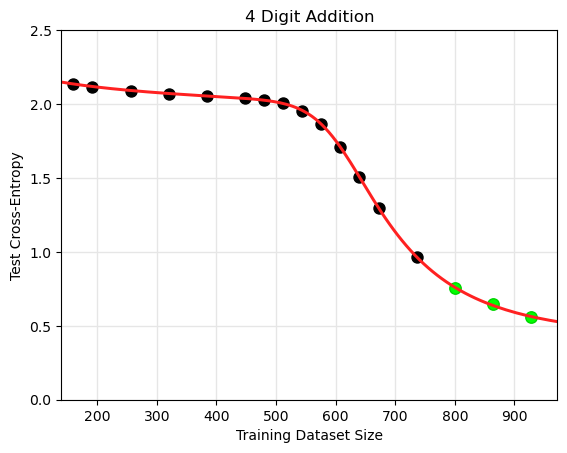
\includegraphics[width=0.48\textwidth]{figures/arithmetic/4_digit_addition__dataset_size.png}
%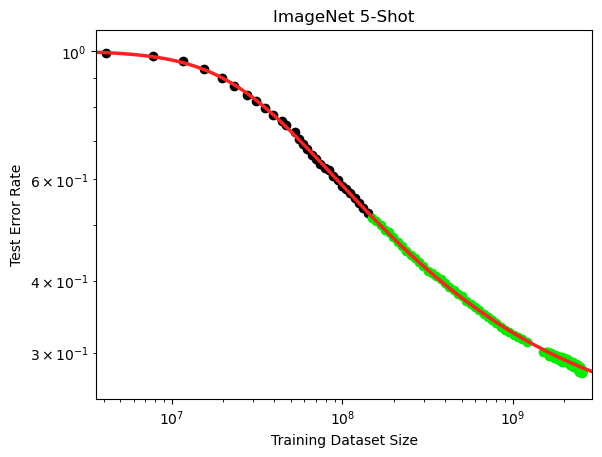
\includegraphics[width=0.497\textwidth]{figures/order_of_magnitude__data_x-axis/imagenet_5___MiX_L_16.png}
%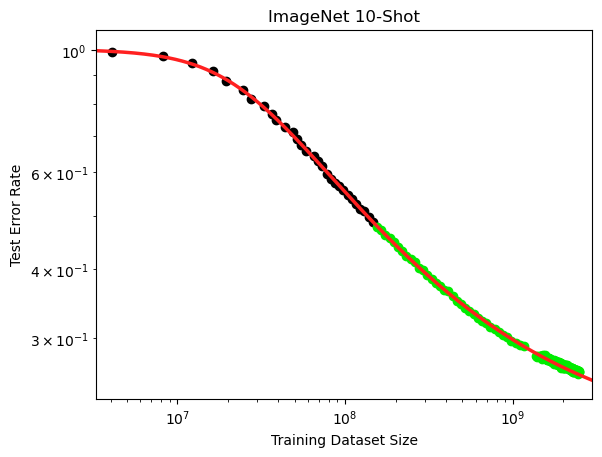
\includegraphics[width=0.48\textwidth]{figures/order_of_magnitude__data_x-axis/imagenet_10___MiX_L_16.png}
%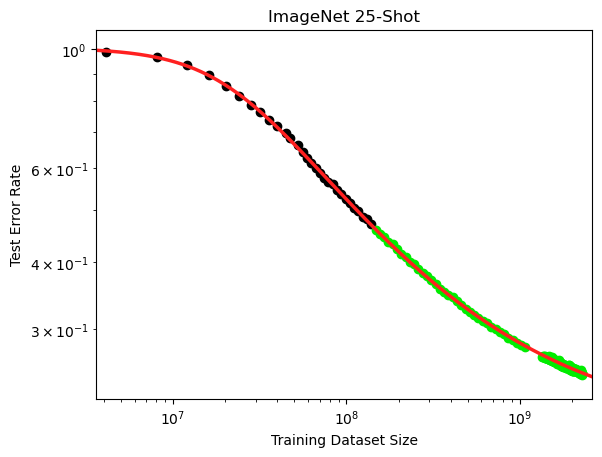
\includegraphics[width=0.497\textwidth]{figures/order_of_magnitude__data_x-axis/imagenet_25___MiX_L_16.png}
%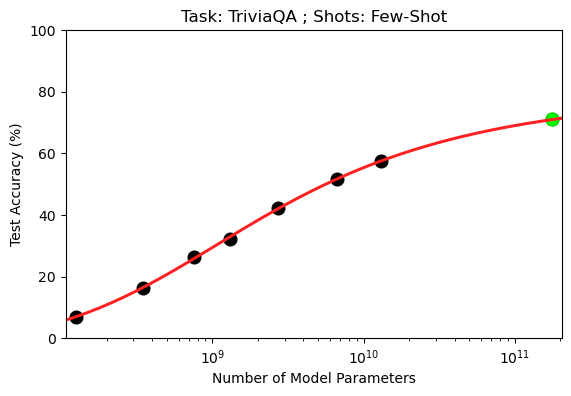
\includegraphics[width=0.4715\textwidth]{figures/gpt-3__parameter_scaling/TriviaQA___Few-Shot.png}

%\hspace{-5mm}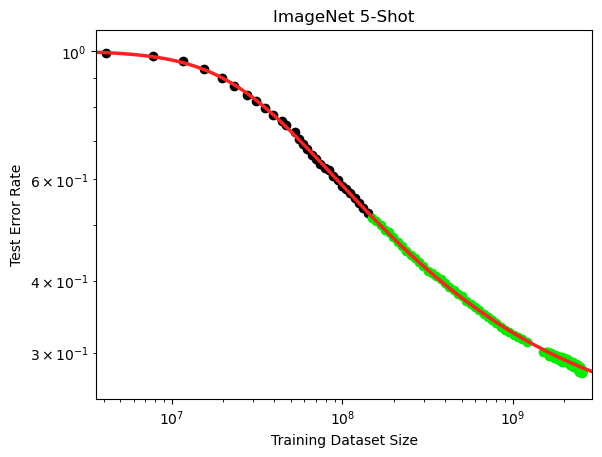
\includegraphics[width=0.65\textwidth]{figures/order_of_magnitude__data_x-axis/imagenet_5___MiX_L_16.png}
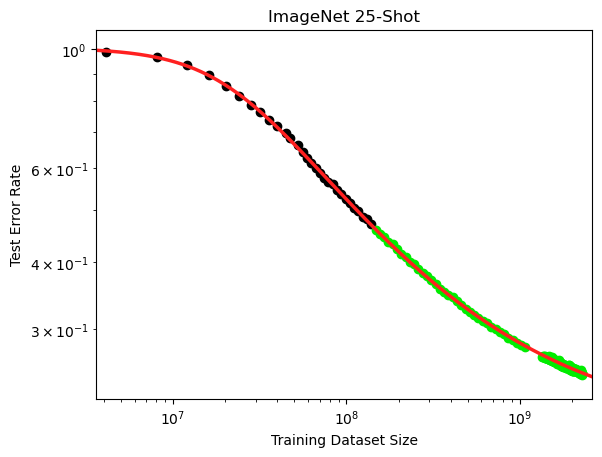
\includegraphics[width=0.71\textwidth]{figures/order_of_magnitude__data_x-axis/imagenet_25___MiX_L_16.png}

%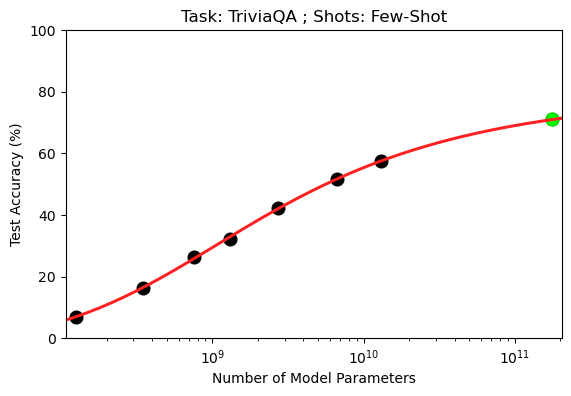
\includegraphics[width=0.62\textwidth]{figures/gpt-3__parameter_scaling/TriviaQA___Few-Shot.png}
%\hspace{1mm}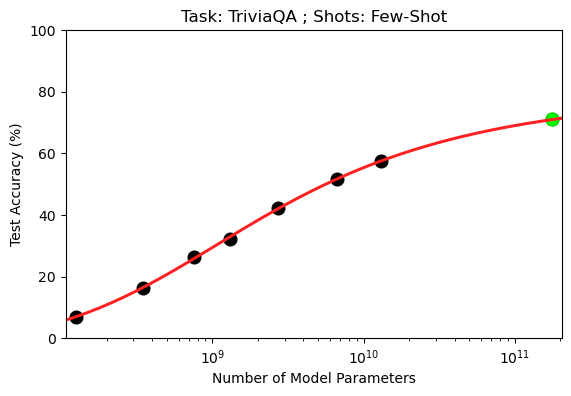
\includegraphics[width=0.71\textwidth]{figures/gpt-3__parameter_scaling/TriviaQA___Few-Shot.png}
%\hspace{6.3mm}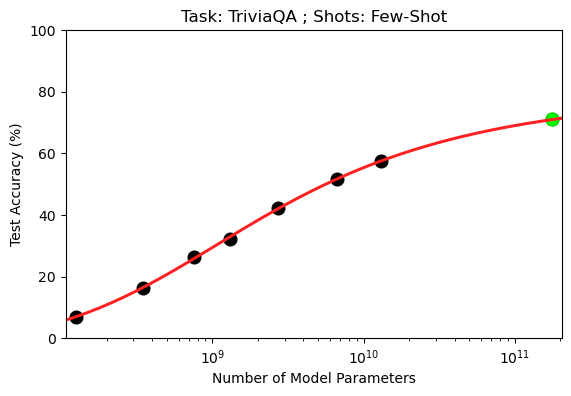
\includegraphics[width=0.6705\textwidth]{figures/gpt-3__parameter_scaling/TriviaQA___Few-Shot.png}
\hspace{5.7mm}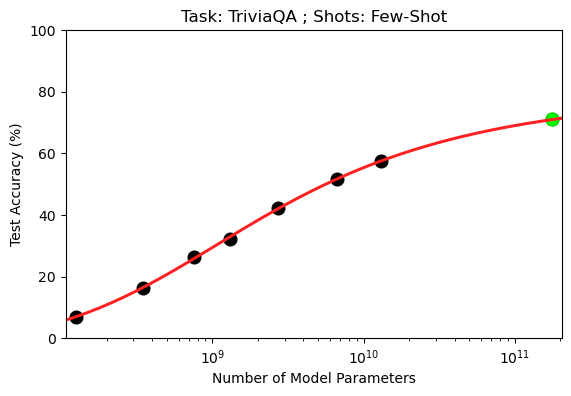
\includegraphics[width=0.6732\textwidth]{figures/gpt-3__parameter_scaling/TriviaQA___Few-Shot.png}
\vspace{-3.55mm}
    \caption{
    BNSL accurately Extrapolating \textbf{Downstream} Performance to Scales that are greater than an Order of Magnitude larger than the maximum (along the x-axis) of the points used for fitting; there are additional similar results in the Appendix. Experimental data of scaling behavior in top plot obtained from scaling laws benchmark of \cite{Alabdulmohsi2022revisiting}; see Appendix \ref{section:extrapolate_oom} for more details. Experimental data of scaling behavior in bottom plot obtained from Table H.1 of GPT-3 arXiv paper \citep{brown2020language}; see Appendix \ref{section:language_tasks__number_of_parameters} for more details. 
    %The bottom plot has a break at 4.11e8 along the x-axis.
    %In Figure \ref{fig:extrapolate_oom}, we show that BNSL accurately extrapolates to scales that are an order of magnitude larger than the maximum (along the x-axis) of the points used for fitting. The upstream task is supervised pretraining of MLP mixers (MiX) \citep{tolstikhin2021mlp} on subsets (i.e. the x-axis of plot) of JFT-300M \citep{sun2017revisiting}. The downstream task is n-shot ImageNet classification (i.e. the y-axis of plot). The experimental data of this scaling behavior is obtained from \cite{Alabdulmohsi2022revisiting}.   
    }
    %\vspace{-3.9mm}
    \label{fig:extrapolate_oom_main_paper}
    \vspace{-1.7mm}
\end{figure*}

%\vspace{-3.9mm}

\FloatBarrier

\vspace{-1.9mm}

\subsection{Reinforcement Learning}
\label{section:reinforcement_learning}

\vspace{-3.25mm}

We show that BNSL accurately models and extrapolates the scaling behaviors of various multi-agent and single-agent reinforcement learning algorithms trained in various environments. In the top left plot and top middle plot and top right plot of Figure \ref{fig:rl_scaling}, BNSL accurately models and extrapolates the scaling behavior of the AlphaZero algorithm trained to play the game Connect Four from Figure 4 and Figure 5 and Figure 3 respectively of \cite{neumann2022scaling}; the x-axes respectively are compute (FLOPs) used for training, training dataset size (states), and number of model parameters. In Figure \ref{fig:rl_scaling} bottom left and bottom right respectively, BNSL accurately models and extrapolates the scaling behavior of the Phasic Policy Gradient (PPG) algorithm \citep{cobbe2021phasic} trained to play the Procgen \citep{cobbe2020leveraging} game called StarPilot and the scaling behavior of the Proximal Policy Optimization (PPO) algorithm \citep{schulman2017proximal} trained to play the Procgen \citep{cobbe2020leveraging} game called Heist.

\vspace{-2.0mm}

In Section \ref{section:ai_alignment}, we find BNSL accurately extrapolates the scaling behavior of a pretrained language model finetuned (i.e. aligned) via Reinforcement Learning from Human Feedback (RLHF) to be helpful from Figure 1 of \cite{bai2022training}.

\vspace{-1.0mm}

\FloatBarrier
\begin{figure*}[hhh]%tbp]
    \centering


%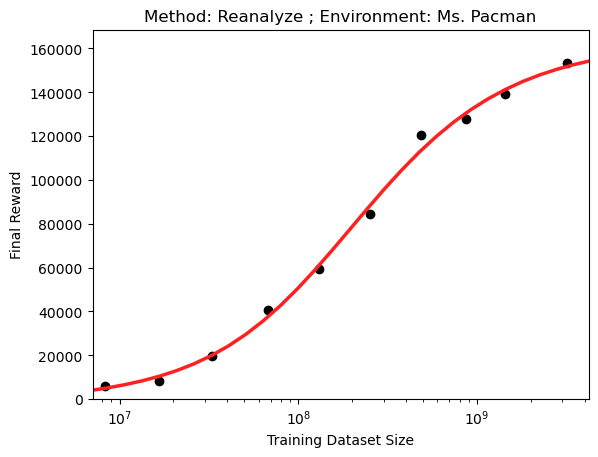
\includegraphics[width=0.45\textwidth]{figures/rl/reanalyze/reanalyze__ms_pacman_dataset_size__fit.png}
%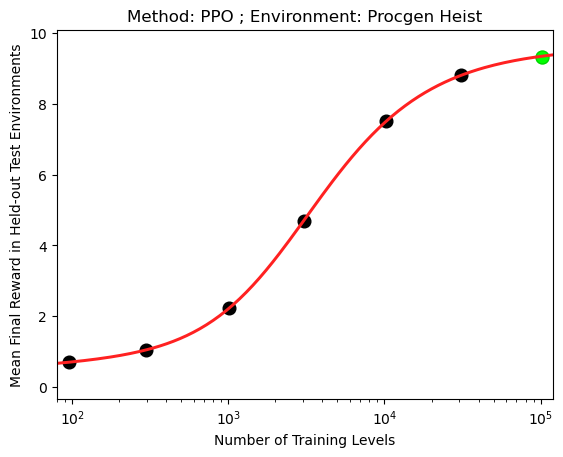
\includegraphics[height=0.345\textwidth]{figures/rl/procgen/Procgen_Heist.png}

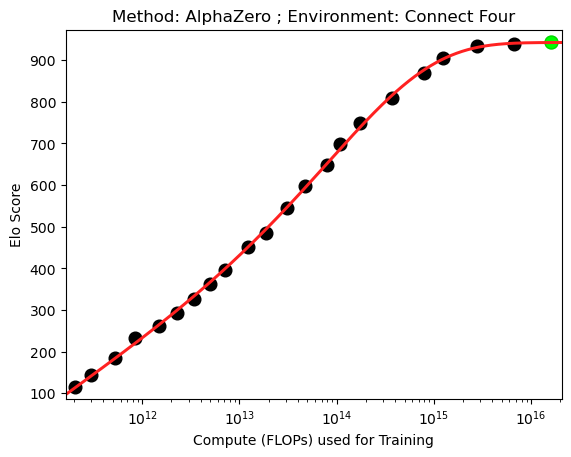
\includegraphics[width=.329\textwidth]{figures/rl/connect_four/connect_four__compute.png}
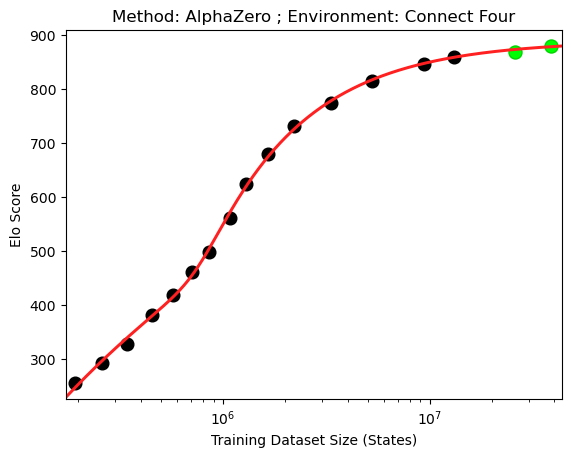
\includegraphics[width=.329\textwidth]{figures/rl/connect_four/connect_four__data.png}
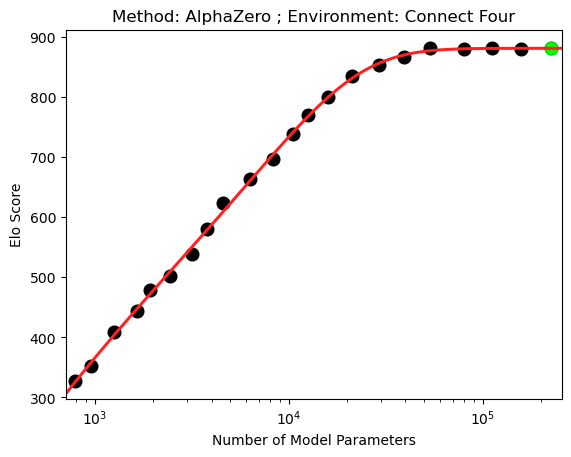
\includegraphics[width=.329\textwidth]{figures/rl/connect_four/connect_four__parameters.png}

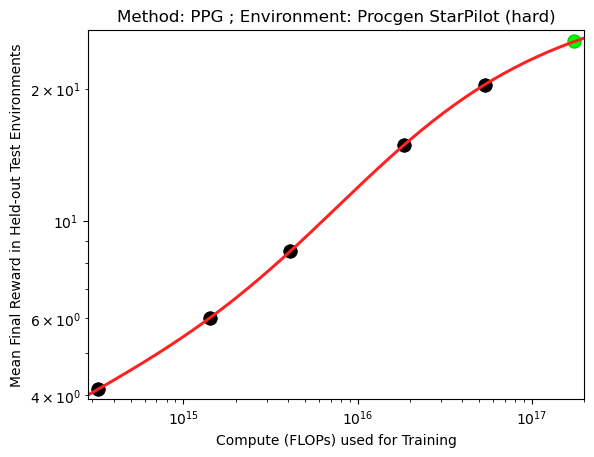
\includegraphics[width=.496\textwidth]{figures/rl/procgen/Procgen_StarPilot_width_compute.png}
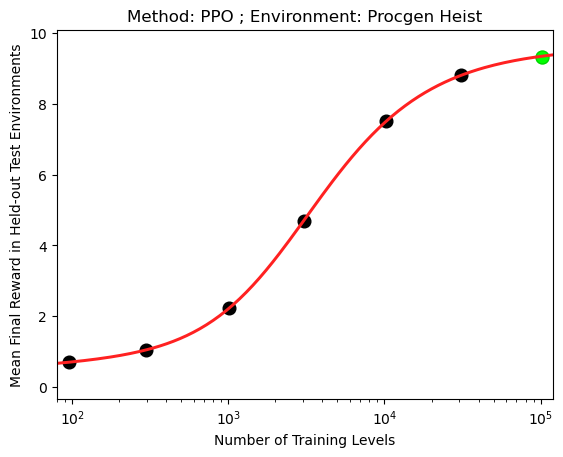
\includegraphics[width=.472\textwidth]{figures/rl/procgen/Procgen_Heist.png}
\vspace{-4.0mm}
    \caption{
    %Fit of BNSL to Reinforcement Learning Scaling Data. Experimental Data of the left plot is from Figure 1 of \cite{schrittwieser2021online}. Experimental Data of the right plot is from Figure 2 of \cite{cobbe2020leveraging}.
    Extrapolation Results of BNSL on Reinforcement Learning Scaling Experimental Data. Experimental data of the top left plot and top middle plot and top right plot is from Figure 4 and Figure 5 and Figure 3 respectively of \cite{neumann2022scaling}. Experimental Data of the bottom left plot is from Figure 1 left of \cite{hilton2023scaling}. Experimental Data of the bottom right plot is from Figure 2 of \cite{cobbe2020leveraging}. Top left and bottom left plot is the compute-optimal Pareto frontier. See Section \ref{section:reinforcement_learning} for more details.
    % 3 params
    % 4 compute
    % 5 data
    }
    \label{fig:rl_scaling}
\end{figure*}
\FloatBarrier

\vspace{-3.1mm}

\subsection{Non-Monotonic Scaling}
\label{section:non-monotonic_scaling}
\vspace{-3.2mm}
We show that BNSL accurately models and extrapolates non-monotonic scaling behaviors that are exhibited by Transformers (\cite{vaswani2017attention}) in double descent \citep{nakkiran2021deep} in Figure \ref{fig:double_descent}. Various other functional forms are mathematically incapable of expressing non-monotonic behaviors (as shown in Section \ref{section:math_proofs}).

\vspace{-3.5mm}

%TODO: mention that transformer was used

\FloatBarrier
\begin{figure*}[h]%tbp]
    \centering


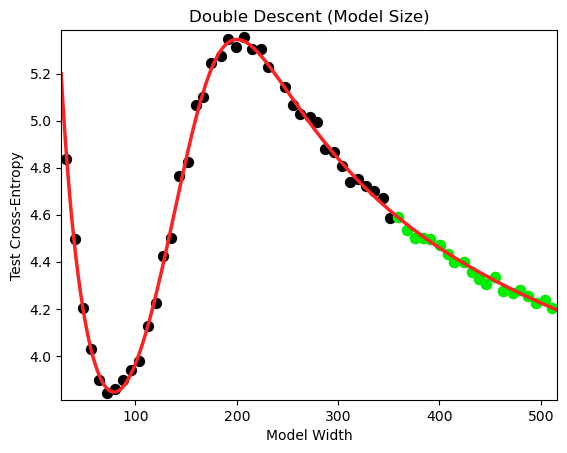
\includegraphics[width=0.496\textwidth]{figures/double_descent/double_descent__model_size.png}
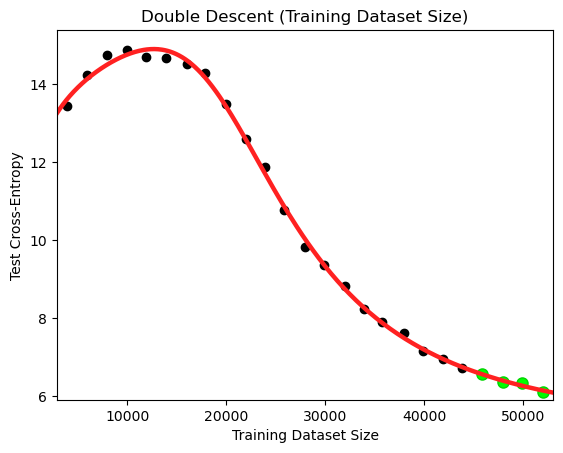
\includegraphics[width=0.496\textwidth]{figures/double_descent/double_descent__dataset_size_1.png}
\vspace{-4.0mm}
    \caption{
    Extrapolation of BNSL on Double Descent. Both plots are of transformers trained to do neural machine translation via minimizing cross-entropy. Experimental data of left figure is obtained from Figure 8 top of \cite{nakkiran2021deep}; ``Model Width" on the x-axis refers to embedding dimension $d_{model}$ of the transformer; note that model width is linearly proportional to number of model parameters, so number of model parameters on the x-axis would yield same results. Experimental data of the right figure is obtained from Figure 11b of \cite{nakkiran2021deep}. The plot on the left contains \textbf{two breaks} of a BNSL fit to the black points. See Section \ref{section:non-monotonic_scaling} for more details.
    }
    \label{fig:double_descent}
\end{figure*}

\vspace{-2.5mm}

\FloatBarrier

\subsection{Inflection Points}
\label{section:Inflection_Points}
\vspace{-3.0mm}
We show that BNSL is capable of modeling and extrapolating the scaling behavior of tasks that have an inflection point on a linear-linear plot such as the task of arithmetic (4-digit addition). Here we model and extrapolate the scaling behavior of a transformer model (\cite{vaswani2017attention}) with respect to the training dataset size on the 4-digit addition task. Various other functional forms are mathematically incapable of expressing inflection points on a linear-linear plot (as shown in Section \ref{section:math_proofs}) and as a result, are mathematically incapable of expressing and modeling inflection points (on a linear-linear plot) that are present in the scaling behavior of 4-digit addition. In Figure \ref{fig:arithmetic} left, we show that BNSL expresses and accurately models the inflection point present in the scaling behavior of 4-digit addition and as a result accurately extrapolates the scaling behavior of 4 digit addition. For further details about the hyperparameters please refer to the Appendix Section \ref{section:Inflection_points_experimental}.

\vspace{-2.0mm}

Also, we additionally find that BNSL accurately models and extrapolates the scaling behavior with number of training
steps on the x-axis in Section \ref{section:steps}.

\vspace{-3.9mm}

%\FloatBarrier
\begin{figure*}[htbp]
    \centering


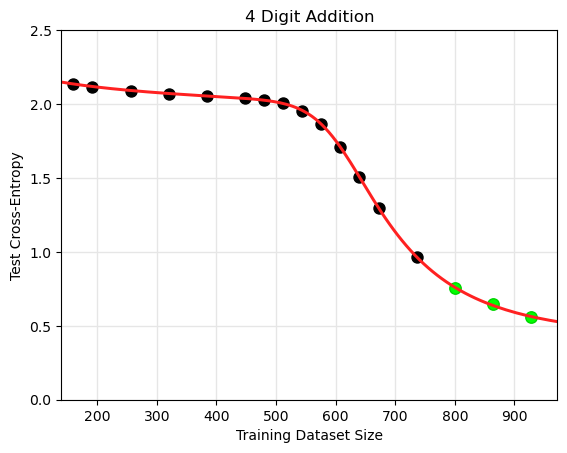
\includegraphics[width=0.496\textwidth]{figures/arithmetic/4_digit_addition__dataset_size.png}
%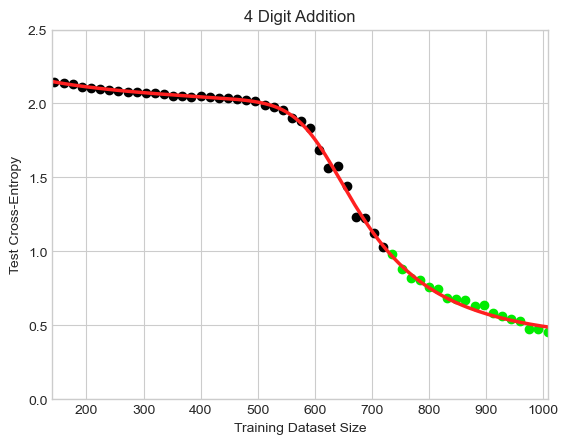
\includegraphics[width=0.48\textwidth]{figures/arithmetic/4_digit_addition__dataset_size__very_first_version.png}
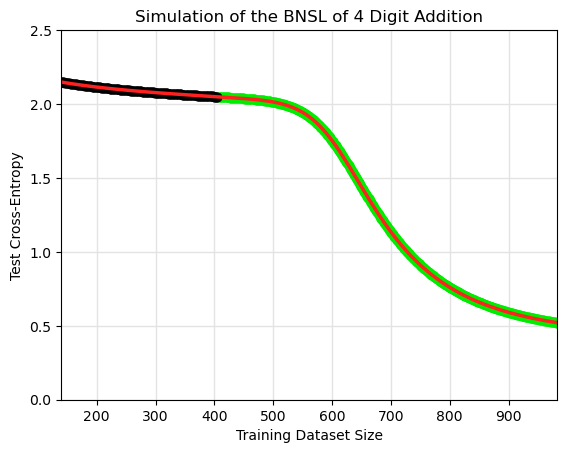
\includegraphics[width=0.496\textwidth]{figures/arithmetic/4_digit_addition__dataset_size__very_first_version__simulation_limit.png}
\vspace{-4.7mm}
    \caption{
    Extrapolation of BNSL on 4 Digit Addition. Note these plots are linear-linear. Each point in left plot is mean of greater than 1000 seeds at that dataset size. In left plot, each point is gathered from a model trained to do task of 4 digit addition. In right plot, each point is gathered from a noiseless simulation of the BNSL of the task of 4 digit addition. See Sections \ref{section:Inflection_Points}, \ref{section:Inflection_points_experimental}, \ref{section:limit_of_agi_superforecasting}, for more details.
    }
    \label{fig:arithmetic}
\end{figure*}
\vspace{-3.0mm}
\FloatBarrier

%\subsection{The Limit of the Predictability of Scaling Behavior}
\vspace{-2.0mm}
\section{The Limit of the Predictability of Scaling Behavior}
\label{section:limit_of_agi_superforecasting}
\vspace{-4.0mm}
We use BNSL to glean insights about the limit of the predictability of scaling behavior. Recent papers \citep{ganguli2022predictability, wei2022emergent} have advertised many tasks as having ``unpredictable" ``emergent" ``phase transition/change" scaling behavior, the most famous of which is the task of arithmetic. In the previous section and in Figure \ref{fig:arithmetic} left, we successfully predicted (i.e. extrapolated) the scaling behavior of 4-digit addition (arithmetic). However, we are only able to accurately extrapolate the scaling behavior if given some points from training runs with a training dataset size of at least 720, and the break in which the scaling behavior of 4-digit addition transitions from one power law to another steeper power-law happens at around training dataset size of 415. 

\vspace{-1.4mm}

Ideally, one would like to be able to extrapolate the entire scaling behavior by fitting only points from before the break. In Figure \ref{fig:arithmetic} right, we use a noiseless simulation of the BNSL of 4-digit addition to show what would happen if one had infinitely many training runs / seeds to average out all the noisy deviation between runs such that one could recover (i.e. learn via a curve-fitting library such as SciPy \citep{virtanen2020scipy}) the learned constants of the BNSL as well as possible. When using this noiseless simulation, we find that we are only able to accurately extrapolate the scaling behavior if given some points from training runs with a training dataset size of at least 415, which is very close to the break. 

%\vspace{-0.4mm}

%This implies that very near to the break there is limit as to how small the maximum of the x-axis of the points used for fitting can be if one wants to perfectly extrapolate the scaling behavior, even if one has infinitely many seeds / training runs. 


%\todo[inline]{TODO: replace maximum with maximum but the wording has to be more clear if maximum is used}

This has a few implications:

\vspace{-1.8mm}

1) When the scaling behavior exhibits greater than 0 breaks that are sufficiently sharp, there is a limit as to how small the maximum (along the x-axis) of the points used for fitting can be if one wants to perfectly extrapolate the scaling behavior, even if one has infinitely many seeds / training runs.

\vspace{-1.8mm}

2) If an additional break of sufficient sharpness happens at a scale that is sufficiently larger than the maximum (along the x-axis) of the points used for fitting, there does not (currently) exist a way to extrapolate the scaling behavior after that additional break.

\vspace{-1.8mm}

3) If a break of sufficient sharpness happens at a scale sufficiently smaller than the maximum (along the x-axis) of the points used for fitting, points smaller (along the x-axis) than that break are often useless for improving extrapolation.

%TODO: Mention it is a one break-point simulation. Mention how the simulation is done.

%\subsection{BIG Bench Emergent}
%Probably will just finish it for rebuttals


%\section{Conclusions}
\noindent{\bf Summary.}

(TODO: This is just the abstract copied; and Surya's

We have presented a smoothly broken power law functional form that accurately models the scaling behaviors (of artificial neural networks) (i.e. how the evaluation metric of interest varies as the amount of compute used for training, number of model parameters, or training dataset size varies) for each task from a very large and diverse set of upstream and downstream (i.e. zero-shot, prompted, and fine-tuned) tasks. These tasks include large-scale vision tasks, large-scale unsupervised language tasks, arithmetic, and reinforcement learning. This functional form yields extrapolations of scaling behavior that often are an order of magnitude more accurate than other functional forms for modeling the scaling behavior of artificial neural networks. Furthermore, this functional form accurately models many scaling behaviors that other functional are mathematically incapable of expressing such as the non-monotonic transitions present in the scaling behavior of phenomena such as double descent and the delayed, sharp inflection points present in the scaling behavior of tasks such as arithmetic.

\noindent{\bf Limitations.} The most notable limitation   

\noindent{\bf Ethical considerations.} A potential negative societal impact could be that  

\noindent{\bf Future work.}
 
%\vspace{-3.95mm}
%\section{Conclusions}
\section{Discussion}
%\vspace{-4.8mm}
%\noindent{\bf Summary.}
We have presented a smoothly broken power law functional form that accurately models and extrapolates the scaling behaviors of artificial neural networks for various architectures and for each of various tasks from a very large and diverse set of upstream and downstream tasks. This set includes large-scale vision, language, audio, video, diffusion, generative modeling, multimodal learning, contrastive learning, AI alignment, robotics, out-of-distribution generalization, continual learning, transfer learning, uncertainty estimation / calibration, out-of-distribution detection, adversarial robustness, distillation, sparsity, retrieval, quantization, pruning, fairness, molecules, computer programming/coding, math word problems, ``emergent" ``phase transitions", arithmetic, unsupervised/self-supervised learning, and reinforcement learning (single agent and multi-agent). When compared to other functional forms for neural scaling behavior, this functional form yields extrapolations of scaling behavior that are considerably more accurate on this set. Additionally, this functional form accurately models and extrapolates scaling behavior that other functional forms are incapable of expressing such as the non-monotonic transitions present in the scaling behavior of phenomena such as double descent and the delayed, sharp inflection points present in the scaling behavior of tasks such as arithmetic. Lastly, we used this functional form to glean insights about the limit of the predictability of scaling behavior.

%\noindent{\bf Future Work.} We place relatively high probability on the claim that variants of smoothly broken power laws (e.g. BNSL) perhaps are the ``true" functional form of the scaling behavior of all(?) things that involve artificial neural networks and encourage the community to work on disproving or further verifying this claim.

%\noindent{\bf Limitations.} A limitation of the current approach is the potential need to collect enough samples of the system's performance (i.e. the (x,y) points required for estimating the scaling laws parameters). A small number of samples may not be sufficient to accurately fit and extrapolate the BNSL functional form, and obtaining a large number of such samples can sometimes be costly.
%\noindent{\bf Limitations.} Among the most significant limitations of the current approach is the potential need for an effective algorithm that allows to collect enough samples of system's performance (i.e. the (x,y) points required for estimating the scaling laws parameters). A small number of samples may not be sufficient to accurately fit and extrapolate the BNSL functional form, but obtaining a large number of such samples can sometimes be costly. %Thus, we need to develop an algorithm for finding cost-efficient sampling trade-off. This is one of the immediate next steps in our future work plans.

\subsubsection*{Ethics Statement}
We place relatively high probability on the claim that variants of smoothly broken power laws perhaps are the ``true" functional form of the scaling behavior of many (all?) things that involve artificial neural networks. Due to the fact that BNSL is a variant of smoothly broken power laws, an ethical concern one might have about our work is that revealing BNSL might differentially \citep{hendrycks2022x} improve A(G)I capabilities progress relative to A(G)I safety/alignment progress. 
A counter-argument is that BNSL will also allow the A(G)I safety/alignment field to extrapolate the scaling behaviors of its methods for aligning A(G)I systems and as a result will also accelerate alignment/safety progress.
Existing scaling laws besides BNSL struggle especially to model downstream performance, e.g.\ on safety-relevant evaluations (especially evaluations (such as interpretability and controllability) that might exhibit non-monotonic scaling behavior in the larger scale systems of the future); we believe our work could differentially help in forecasting emergence of novel capabilities (such as reasoning \citep{wei2022chain}) or behaviors (such as deception or dishonesty \citep{evans2021truthful,lin2021truthfulqa}), and thus help avoid unpleasant surprises.

A potential limitation of the current approach is the need to collect enough samples of the system’s performance (i.e. the (x,y) points required for estimating the scaling laws parameters). A small number of samples sometimes may not be sufficient to accurately fit and extrapolate the BNSL functional form, and obtaining a large number of such samples can sometimes be costly. This has the ethical implication that entities with more compute to gather more points maybe will have considerably more accurate extrapolations of scaling behavior than entities with less compute. As a result, entities with less compute (e.g. academia) maybe will have less foresight than entities with more compute (e.g. Big Tech), which could maybe exacerbate the gap between entities with more compute (e.g. Big Tech) and entities with less compute (e.g. academia).

\subsubsection*{Acknowledgments}
We are thankful for useful feedback and assistance from Kartik Ahuja, Ibrahim Alabdulmohsin, Ankesh Anand, Jacob Buckman, Guillaume Dumas, Leo Gao, Andy Jones, Behnam Neyshabur, Gabriel Prato, Stephen Roller, Michael Trazzi, Tony Wu and others.

%\noindent{\bf Future work.}

\newpage

%\subsubsection*{Author Contributions}
%If you'd like to, you may include  a section for author contributions as is done in many journals. This is optional and at the discretion of the authors.

%\subsubsection*{Acknowledgments}
%Use unnumbered third level headings for the acknowledgments. All acknowledgments, including those to funding agencies, go at the end of the paper.


% This pushes the appendix to next page
\clearpage 
\appendix
%\section{Appendix}
You may include other additional sections here.

\section{Experimental details of \ref{section:Inflection_Points}}
We perform an extensive set of experiments to model and extrapolate the scaling behavior for the 4-digit arithmetic addition task with respect to the training dataset size.We set the batch size equal to the training dataset size. We do not use dropout or a learning rate decay here. For our experiments we train the transformer model using the following set of hyperparameters:
\begin{table}[hbt!]
    \centering
    \begin{tabular}{c|c}
         Model Embedding size & 128 \\
         Number of heads & 2 \\
         Number of layers & 1 \\
         Learning rate & 0.0001\\
         Dropout Probability & 0.0\\
         Test set size & 1000\\
    \end{tabular}
    \caption{Hyperparameters for 4-digit addition task}
    \label{tab:my_label}
\end{table}

\section{All Tables and Plots on the Scaling Laws Benchmark of \citet{Alabdulmohsi2022revisiting}}
\label{all_scaling_laws}

\subsection{Table of Extrapolations}

\FloatBarrier

\begin{table}
\tiny
\setlength\tabcolsep{3.1pt} 
\begin{tabular}
%{p{.02\textwidth}p{.165\textwidth}p{.095\textwidth}p{.01\textwidth}p{.01\textwidth}p{.099\textwidth}p{.099\textwidth}p{.099\textwidth}p{.099\textwidth}p{.099\textwidth}}
{p{.021\textwidth}p{.165\textwidth}p{.111\textwidth}p{.028\textwidth}p{.022\textwidth}p{.099\textwidth}p{.099\textwidth}p{.099\textwidth}p{.099\textwidth}p{.099\textwidth}}
%\begin{tabular}{llllrrrrrrrrrrrrl}
Domain & \hspace{.9cm}Task & Model & Train Points & Test Points & M1 \downarrow & M2 \downarrow & M3 \downarrow & M4 \downarrow & BNSL \downarrow \\
\hline
BB & date understanding, 1-shot & 2.62e+8 Param & 19 & 24 & 3.19e-2 ± 9.6e-4 & 3.09e-2 ± 9.2e-4 & \bfseries 4.67e-3 ± 1.4e-4 & 1.49e-2 ± 5.9e-4 & 4.96e-3 ± 4.8e-5 \\
BB & date understanding, 2-shot & 2.62e+8 Param & 19 & 24 & 2.86e-2 ± 6.2e-4 & 2.44e-2 ± 5.6e-4 & 4.83e-3 ± 4.1e-4 & 1.58e-2 ± 5.0e-4 & \bfseries 2.55e-3 ± 6.2e-4 \\
BB & linguistic mappings, 1-shot & 2.62e+8 Param & 19 & 24 & 1.66e-2 ± 5.5e-4 & \bfseries 1.41e-2 ± 4.7e-4 & 1.66e-2 ± 5.5e-4 & 1.57e-2 ± 4.8e-4 & 2.22e-2 ± 8.2e-4 \\
BB & linguistic mappings, 2-shot & 2.62e+8 Param & 19 & 24 & 1.70e-2 ± 6.5e-4 & 1.30e-2 ± 5.4e-4 & 1.70e-2 ± 6.5e-4 & 9.25e-3 ± 5.1e-4 & \bfseries 8.09e-3 ± 5.1e-4 \\
BB & mult data wrangling, 1-shot & 2.62e+8 Param & 19 & 24 & 1.07e-2 ± 1.0e-3 & 6.71e-3 ± 7.6e-4 & 1.07e-2 ± 1.0e-3 & 8.27e-3 ± 8.4e-4 & \bfseries 6.17e-3 ± 8.4e-4 \\
BB & mult data wrangling, 2-shot & 2.62e+8 Param & 19 & 24 & 1.57e-2 ± 1.5e-3 & 7.22e-3 ± 8.9e-4 & 1.57e-2 ± 1.5e-3 & \bfseries 5.01e-3 ± 5.0e-4 & 5.45e-3 ± 9.2e-4 \\
BB & qa wikidata, 1-shot & 2.62e+8 Param & 19 & 24 & \bfseries 4.27e-3 ± 8.9e-4 & 5.14e-3 ± 5.3e-4 & 4.27e-3 ± 8.9e-4 & 5.05e-3 ± 5.6e-4 & 4.34e-3 ± 6.1e-4 \\
BB & qa wikidata, 2-shot & 2.62e+8 Param & 19 & 24 & 4.39e-3 ± 7.0e-4 & 7.35e-3 ± 6.1e-4 & 4.39e-3 ± 7.0e-4 & 7.12e-3 ± 6.0e-4 & \bfseries 4.20e-3 ± 6.0e-4 \\
BB & unit conversion, 1-shot & 2.62e+8 Param & 19 & 24 & 8.30e-3 ± 4.4e-4 & 6.77e-3 ± 4.0e-4 & \bfseries 1.48e-3 ± 2.7e-4 & 2.32e-3 ± 2.3e-4 & 6.32e-3 ± 2.5e-4 \\
BB & unit conversion, 2-shot & 2.62e+8 Param & 19 & 24 & 1.07e-2 ± 4.4e-4 & 9.15e-3 ± 4.7e-4 & 7.50e-3 ± 5.5e-4 & \bfseries 2.83e-3 ± 4.8e-4 & 5.21e-3 ± 5.2e-4 \\
IC & Birds 200 10-shot & BiT/101/3 & 57 & 107 & 9.13e-2 ± 2.8e-3 & 9.13e-2 ± 2.8e-3 & 9.13e-2 ± 2.8e-3 & 2.49e-2 ± 1.2e-3 & \bfseries 3.79e-3 ± 1.1e-3 \\
IC & Birds 200 10-shot & BiT/50/1 & 70 & 469 & 6.88e-2 ± 7.5e-4 & 6.88e-2 ± 7.5e-4 & 5.24e-2 ± 6.2e-4 & 2.48e-2 ± 5.1e-4 & \bfseries 4.96e-3 ± 3.9e-4 \\
IC & Birds 200 10-shot & MiX/B/16 & 69 & 383 & 9.15e-2 ± 1.1e-3 & 9.15e-2 ± 1.1e-3 & 3.95e-2 ± 7.0e-4 & 4.14e-2 ± 7.8e-4 & \bfseries 9.98e-3 ± 7.0e-4 \\
IC & Birds 200 10-shot & MiX/L/16 & 63 & 211 & 5.51e-2 ± 1.4e-3 & 5.51e-2 ± 1.4e-3 & 5.51e-2 ± 1.4e-3 & 4.59e-2 ± 1.6e-3 & \bfseries 8.41e-3 ± 1.3e-3 \\
IC & Birds 200 10-shot & ViT/B/16 & 65 & 316 & 6.77e-2 ± 1.1e-3 & 6.77e-2 ± 1.1e-3 & 3.52e-2 ± 8.1e-4 & 1.87e-2 ± 7.2e-4 & \bfseries 9.81e-3 ± 8.1e-4 \\
IC & Birds 200 10-shot & ViT/S/16 & 54 & 133 & 3.95e-2 ± 1.2e-3 & 3.95e-2 ± 1.2e-3 & 3.74e-2 ± 1.1e-3 & \bfseries 9.81e-3 ± 5.4e-4 & 1.51e-2 ± 8.4e-4 \\
IC & Birds 200 25-shot & BiT/101/3 & 53 & 78 & 9.41e-2 ± 3.2e-3 & 9.41e-2 ± 3.2e-3 & 9.41e-2 ± 3.2e-3 & 5.09e-2 ± 1.8e-3 & \bfseries 7.24e-3 ± 1.6e-3 \\
IC & Birds 200 25-shot & BiT/50/1 & 69 & 452 & 1.10e-1 ± 1.0e-3 & 7.29e-2 ± 8.0e-4 & 1.52e-2 ± 4.9e-4 & 1.63e-2 ± 5.1e-4 & \bfseries 8.00e-3 ± 6.1e-4 \\
IC & Birds 200 25-shot & MiX/B/16 & 67 & 293 & 1.40e-1 ± 1.9e-3 & 1.40e-1 ± 1.9e-3 & 6.93e-2 ± 1.2e-3 & 1.85e-2 ± 6.3e-4 & \bfseries 5.02e-3 ± 6.2e-4 \\
IC & Birds 200 25-shot & MiX/L/16 & 63 & 196 & 1.12e-1 ± 2.0e-3 & 1.12e-1 ± 2.0e-3 & 1.12e-1 ± 2.0e-3 & 4.88e-2 ± 1.8e-3 & \bfseries 1.05e-2 ± 1.7e-3 \\
IC & Birds 200 25-shot & ViT/B/16 & 64 & 271 & 9.02e-2 ± 1.6e-3 & 9.02e-2 ± 1.6e-3 & 3.75e-2 ± 1.0e-3 & 1.52e-2 ± 5.8e-4 & \bfseries 5.87e-3 ± 6.1e-4 \\
IC & Birds 200 25-shot & ViT/S/16 & 51 & 100 & 5.06e-2 ± 1.4e-3 & 5.06e-2 ± 1.4e-3 & 4.96e-2 ± 1.4e-3 & 3.28e-2 ± 1.1e-3 & \bfseries 1.21e-2 ± 8.5e-4 \\
IC & Birds 200 5-shot & BiT/101/3 & 62 & 180 & 8.17e-2 ± 2.0e-3 & 8.17e-2 ± 2.0e-3 & 8.17e-2 ± 2.0e-3 & 3.00e-2 ± 1.2e-3 & \bfseries 6.08e-3 ± 1.1e-3 \\
IC & Birds 200 5-shot & BiT/50/1 & 71 & 517 & 5.44e-2 ± 5.6e-4 & 5.44e-2 ± 5.6e-4 & 5.44e-2 ± 5.6e-4 & 2.63e-2 ± 5.4e-4 & \bfseries 5.79e-3 ± 3.7e-4 \\
IC & Birds 200 5-shot & MiX/B/16 & 71 & 494 & 8.27e-2 ± 1.0e-3 & 8.27e-2 ± 1.0e-3 & 5.49e-2 ± 7.8e-4 & 1.86e-2 ± 5.0e-4 & \bfseries 5.74e-3 ± 4.7e-4 \\
IC & Birds 200 5-shot & MiX/L/16 & 67 & 326 & 5.68e-2 ± 1.4e-3 & 5.68e-2 ± 1.4e-3 & 5.68e-2 ± 1.4e-3 & 2.65e-2 ± 9.0e-4 & \bfseries 5.06e-3 ± 6.4e-4 \\
IC & Birds 200 5-shot & ViT/B/16 & 65 & 284 & 3.40e-2 ± 8.9e-4 & 3.40e-2 ± 8.9e-4 & 3.40e-2 ± 8.9e-4 & 1.26e-2 ± 5.3e-4 & \bfseries 6.32e-3 ± 5.8e-4 \\
IC & Birds 200 5-shot & ViT/S/16 & 57 & 150 & 2.75e-2 ± 7.9e-4 & 2.75e-2 ± 7.9e-4 & 2.75e-2 ± 7.9e-4 & 1.56e-2 ± 5.9e-4 & \bfseries 6.93e-3 ± 4.8e-4 \\
IC & CIFAR-100 10-shot & BiT/101/3 & 47 & 60 & 8.57e-2 ± 3.8e-3 & 8.57e-2 ± 3.8e-3 & 8.25e-2 ± 3.7e-3 & 9.28e-2 ± 3.9e-3 & \bfseries 1.53e-2 ± 2.9e-3 \\
IC & CIFAR-100 10-shot & BiT/50/1 & 62 & 192 & 7.44e-2 ± 1.5e-3 & 1.24e-2 ± 5.8e-4 & 2.08e-2 ± 7.2e-4 & 1.23e-2 ± 5.7e-4 & \bfseries 9.74e-3 ± 7.1e-4 \\
IC & CIFAR-100 10-shot & MiX/B/16 & 65 & 248 & 8.77e-2 ± 1.9e-3 & 8.77e-2 ± 1.9e-3 & 2.71e-2 ± 1.2e-3 & 2.60e-2 ± 1.2e-3 & \bfseries 8.61e-3 ± 9.5e-4 \\
IC & CIFAR-100 10-shot & MiX/L/16 & 67 & 313 & 1.05e-1 ± 3.1e-3 & 1.05e-1 ± 3.1e-3 & 4.85e-2 ± 2.6e-3 & 4.76e-2 ± 1.7e-3 & \bfseries 1.55e-2 ± 1.6e-3 \\
IC & CIFAR-100 10-shot & ViT/B/16 & 67 & 354 & 8.98e-2 ± 2.0e-3 & 8.98e-2 ± 2.0e-3 & 8.98e-2 ± 2.0e-3 & 5.60e-2 ± 1.8e-3 & \bfseries 1.73e-2 ± 1.8e-3 \\
IC & CIFAR-100 10-shot & ViT/S/16 & 67 & 450 & 6.84e-2 ± 1.1e-3 & 2.11e-2 ± 6.6e-4 & 3.35e-2 ± 8.6e-4 & 2.47e-2 ± 7.4e-4 & \bfseries 1.15e-2 ± 7.5e-4 \\
IC & CIFAR-100 25-shot & BiT/101/3 & 41 & 38 & 8.77e-2 ± 5.6e-3 & 8.77e-2 ± 5.6e-3 & 4.44e-2 ± 3.5e-3 & 4.29e-2 ± 3.4e-3 & \bfseries 9.32e-3 ± 3.0e-3 \\
IC & CIFAR-100 25-shot & BiT/50/1 & 55 & 109 & 7.31e-2 ± 2.0e-3 & 2.35e-2 ± 1.5e-3 & 3.65e-2 ± 1.8e-3 & 2.36e-2 ± 1.5e-3 & \bfseries 2.00e-2 ± 1.8e-3 \\
IC & CIFAR-100 25-shot & MiX/B/16 & 64 & 202 & 1.08e-1 ± 2.3e-3 & 4.75e-2 ± 1.6e-3 & 2.10e-2 ± 9.4e-4 & 2.08e-2 ± 9.3e-4 & \bfseries 8.15e-3 ± 1.1e-3 \\
IC & CIFAR-100 25-shot & MiX/L/16 & 62 & 185 & 9.79e-2 ± 2.2e-3 & 9.79e-2 ± 2.2e-3 & 3.67e-2 ± 1.7e-3 & 2.79e-2 ± 1.3e-3 & \bfseries 8.47e-3 ± 1.6e-3 \\
IC & CIFAR-100 25-shot & ViT/B/16 & 66 & 355 & 1.07e-1 ± 1.9e-3 & 1.07e-1 ± 1.9e-3 & 6.54e-2 ± 1.6e-3 & \bfseries 4.81e-2 ± 1.4e-3 & 1.20e-1 ± 1.4e-3 \\
IC & CIFAR-100 25-shot & ViT/S/16 & 66 & 416 & 8.03e-2 ± 1.2e-3 & 2.19e-2 ± 7.4e-4 & 3.13e-2 ± 8.4e-4 & 2.19e-2 ± 7.0e-4 & \bfseries 1.34e-2 ± 8.5e-4 \\
IC & CIFAR-100 5-shot & BiT/101/3 & 47 & 59 & 5.94e-2 ± 3.2e-3 & 5.94e-2 ± 3.2e-3 & 5.94e-2 ± 3.2e-3 & 4.57e-2 ± 2.8e-3 & \bfseries 1.58e-2 ± 2.6e-3 \\
IC & CIFAR-100 5-shot & BiT/50/1 & 57 & 98 & 4.87e-2 ± 1.3e-3 & 4.87e-2 ± 1.3e-3 & \bfseries 1.69e-2 ± 8.8e-4 & 4.91e-2 ± 1.3e-3 & 1.95e-2 ± 1.0e-3 \\
IC & CIFAR-100 5-shot & MiX/B/16 & 66 & 304 & 7.07e-2 ± 1.2e-3 & 7.07e-2 ± 1.2e-3 & 2.78e-2 ± 8.4e-4 & 2.05e-2 ± 7.4e-4 & \bfseries 6.77e-3 ± 6.3e-4 \\
IC & CIFAR-100 5-shot & MiX/L/16 & 67 & 312 & 7.06e-2 ± 1.6e-3 & 7.06e-2 ± 1.6e-3 & 4.17e-2 ± 1.4e-3 & 3.14e-2 ± 1.1e-3 & \bfseries 1.18e-2 ± 1.3e-3 \\
IC & CIFAR-100 5-shot & ViT/B/16 & 67 & 352 & 6.27e-2 ± 1.6e-3 & 6.27e-2 ± 1.6e-3 & 6.27e-2 ± 1.6e-3 & 5.11e-2 ± 1.4e-3 & \bfseries 1.19e-2 ± 1.2e-3 \\
IC & CIFAR-100 5-shot & ViT/S/16 & 70 & 710 & 6.93e-2 ± 1.2e-3 & \bfseries 2.84e-2 ± 8.2e-4 & 3.88e-2 ± 8.0e-4 & 3.09e-2 ± 7.5e-4 & 6.40e-2 ± 7.7e-4 \\
IC & Caltech101 10-shot & BiT/101/3 & 21 & 14 & 3.07e-1 ± 2.0e-2 & 3.07e-1 ± 2.0e-2 & 1.51e-1 ± 1.3e-2 & 3.54e-2 ± 6.3e-3 & \bfseries 6.42e-3 ± 5.8e-3 \\
IC & Caltech101 10-shot & BiT/50/1 & 33 & 16 & 3.29e-1 ± 1.6e-2 & 7.68e-2 ± 5.0e-3 & 1.13e-1 ± 6.0e-3 & 6.31e-2 ± 4.4e-3 & \bfseries 5.37e-3 ± 2.2e-3 \\
IC & Caltech101 10-shot & MiX/B/16 & 14 & 12 & 1.35e-1 ± 1.4e-2 & 1.35e-1 ± 1.4e-2 & 1.35e-1 ± 1.4e-2 & 2.11e-1 ± 1.7e-2 & \bfseries 3.72e-2 ± 9.7e-3 \\
IC & Caltech101 10-shot & MiX/L/16 & 12 & 11 & 1.25e-1 ± 1.3e-2 & 1.25e-1 ± 1.3e-2 & 1.25e-1 ± 1.3e-2 & 1.92e-1 ± 1.6e-2 & \bfseries 3.73e-2 ± 1.5e-2 \\
IC & Caltech101 10-shot & ViT/B/16 & 34 & 33 & 7.76e-2 ± 4.3e-3 & 7.76e-2 ± 4.3e-3 & 3.11e-2 ± 3.0e-3 & 5.54e-2 ± 4.3e-3 & \bfseries 1.67e-2 ± 5.4e-3 \\
IC & Caltech101 10-shot & ViT/S/16 & 43 & 55 & 1.95e-1 ± 6.0e-3 & 3.41e-2 ± 2.9e-3 & \bfseries 2.40e-2 ± 2.0e-3 & 3.95e-2 ± 3.1e-3 & 3.31e-2 ± 5.3e-3 \\
IC & Caltech101 25-shot & BiT/101/3 & 10 & 3 & 1.15e-1 ± 6.5e-3 & 1.15e-1 ± 6.5e-3 & 1.15e-1 ± 6.5e-3 & 5.23e-2 ± 2.7e-3 & \bfseries 1.13e-2 ± 8.0e-3 \\
IC & Caltech101 25-shot & BiT/50/1 & 28 & 16 & 3.60e-1 ± 1.9e-2 & 8.80e-2 ± 5.5e-3 & 1.43e-1 ± 7.6e-3 & 5.95e-2 ± 4.1e-3 & \bfseries 2.13e-3 ± 1.6e-3 \\
IC & Caltech101 25-shot & MiX/B/16 & 13 & 11 & 8.28e-2 ± 1.2e-2 & 8.28e-2 ± 1.2e-2 & 8.28e-2 ± 1.2e-2 & 1.74e-1 ± 1.7e-2 & \bfseries 2.83e-2 ± 1.3e-2 \\
IC & Caltech101 25-shot & MiX/L/16 & 12 & 12 & 9.66e-2 ± 1.0e-2 & 9.66e-2 ± 1.0e-2 & 9.66e-2 ± 1.0e-2 & 1.03e-1 ± 9.5e-3 & \bfseries 1.98e-2 ± 1.3e-2 \\
IC & Caltech101 25-shot & ViT/B/16 & 27 & 28 & 1.03e-1 ± 5.6e-3 & 3.33e-2 ± 2.5e-3 & 4.46e-2 ± 3.6e-3 & 4.24e-2 ± 3.6e-3 & \bfseries 6.37e-3 ± 5.4e-3 \\
IC & Caltech101 25-shot & ViT/S/16 & 41 & 54 & 1.77e-1 ± 5.4e-3 & 3.79e-2 ± 3.1e-3 & 2.80e-2 ± 1.8e-3 & \bfseries 2.35e-2 ± 2.3e-3 & 2.38e-2 ± 4.7e-3 \\
IC & Caltech101 5-shot & BiT/101/3 & 16 & 13 & 2.12e-1 ± 1.2e-2 & 2.12e-1 ± 1.2e-2 & 2.12e-1 ± 1.2e-2 & 8.82e-2 ± 5.0e-3 & \bfseries 3.17e-3 ± 4.3e-3 \\
IC & Caltech101 5-shot & BiT/50/1 & 46 & 54 & 2.34e-1 ± 6.1e-3 & 4.13e-2 ± 2.1e-3 & 1.61e-2 ± 1.3e-3 & 4.49e-2 ± 2.1e-3 & \bfseries 1.33e-2 ± 2.2e-3 \\
IC & Caltech101 5-shot & MiX/B/16 & 24 & 19 & 2.43e-1 ± 1.2e-2 & 2.43e-1 ± 1.2e-2 & 2.35e-1 ± 1.1e-2 & 1.23e-1 ± 6.0e-3 & \bfseries 3.59e-3 ± 1.9e-3 \\
IC & Caltech101 5-shot & MiX/L/16 & 14 & 13 & 1.38e-1 ± 9.7e-3 & 1.38e-1 ± 9.7e-3 & 1.38e-1 ± 9.7e-3 & 3.19e-2 ± 2.6e-3 & \bfseries 3.19e-2 ± 1.1e-2 \\
IC & Caltech101 5-shot & ViT/B/16 & 38 & 41 & 1.10e-1 ± 6.3e-3 & 1.10e-1 ± 6.3e-3 & 6.02e-2 ± 4.7e-3 & 6.59e-2 ± 4.7e-3 & \bfseries 2.33e-2 ± 6.0e-3 \\
IC & Caltech101 5-shot & ViT/S/16 & 49 & 82 & 1.90e-1 ± 4.7e-3 & 3.82e-2 ± 2.6e-3 & 5.04e-2 ± 2.9e-3 & 4.06e-2 ± 2.7e-3 & \bfseries 2.47e-2 ± 3.8e-3 \\
IC & ImageNet 10-shot & BiT/101/3 & 60 & 118 & 1.27e-1 ± 2.0e-3 & 1.27e-1 ± 2.0e-3 & 7.36e-2 ± 1.1e-3 & 2.13e-2 ± 5.8e-4 & \bfseries 5.95e-3 ± 5.5e-4 \\
IC & ImageNet 10-shot & BiT/50/1 & 68 & 262 & 9.54e-2 ± 7.2e-4 & 9.54e-2 ± 7.2e-4 & \bfseries 5.75e-3 ± 2.0e-4 & 1.77e-2 ± 2.7e-4 & 8.93e-3 ± 2.7e-4 \\
IC & ImageNet 10-shot & MiX/B/16 & 69 & 329 & 9.34e-2 ± 7.9e-4 & 9.34e-2 ± 7.9e-4 & 3.37e-2 ± 2.9e-4 & 1.80e-2 ± 2.7e-4 & \bfseries 5.88e-3 ± 2.5e-4 \\
IC & ImageNet 10-shot & MiX/L/16 & 66 & 249 & 9.83e-2 ± 1.3e-3 & 9.83e-2 ± 1.3e-3 & 9.83e-2 ± 1.3e-3 & 9.48e-3 ± 2.4e-4 & \bfseries 3.81e-3 ± 2.9e-4 \\
IC & ImageNet 10-shot & ViT/B/16 & 67 & 289 & 4.62e-2 ± 7.1e-4 & 4.62e-2 ± 7.1e-4 & 4.62e-2 ± 7.1e-4 & 3.43e-2 ± 4.4e-4 & \bfseries 2.85e-3 ± 2.7e-4 \\
IC & ImageNet 10-shot & ViT/S/16 & 65 & 310 & 4.74e-2 ± 5.6e-4 & 4.74e-2 ± 5.6e-4 & 1.66e-2 ± 2.5e-4 & 1.14e-2 ± 2.4e-4 & \bfseries 1.97e-3 ± 1.4e-4 \\
IC & ImageNet 25-shot & BiT/101/3 & 57 & 100 & 1.42e-1 ± 2.3e-3 & 1.42e-1 ± 2.3e-3 & 6.67e-2 ± 9.1e-4 & 2.18e-2 ± 7.0e-4 & \bfseries 4.86e-3 ± 6.2e-4 \\
IC & ImageNet 25-shot & BiT/50/1 & 68 & 263 & 1.17e-1 ± 9.2e-4 & 1.17e-1 ± 9.2e-4 & \bfseries 4.06e-3 ± 1.7e-4 & 1.70e-2 ± 2.5e-4 & 8.14e-3 ± 2.4e-4 \\
IC & ImageNet 25-shot & MiX/B/16 & 68 & 284 & 9.59e-2 ± 9.3e-4 & 9.59e-2 ± 9.3e-4 & 5.39e-2 ± 4.9e-4 & 1.47e-2 ± 2.7e-4 & \bfseries 2.86e-3 ± 2.3e-4 \\
IC & ImageNet 25-shot & MiX/L/16 & 66 & 226 & 1.03e-1 ± 1.3e-3 & 1.03e-1 ± 1.3e-3 & 1.03e-1 ± 1.3e-3 & 6.09e-3 ± 2.5e-4 & \bfseries 1.94e-3 ± 2.6e-4 \\
IC & ImageNet 25-shot & ViT/B/16 & 67 & 289 & 5.17e-2 ± 8.8e-4 & 5.17e-2 ± 8.8e-4 & 5.17e-2 ± 8.8e-4 & 3.26e-2 ± 5.4e-4 & \bfseries 6.91e-3 ± 4.3e-4 \\
IC & ImageNet 25-shot & ViT/S/16 & 65 & 311 & 5.52e-2 ± 4.4e-4 & 4.12e-2 ± 3.4e-4 & 9.65e-3 ± 2.3e-4 & 1.16e-2 ± 2.2e-4 & \bfseries 3.09e-3 ± 2.4e-4 \\
IC & ImageNet 5-shot & BiT/101/3 & 60 & 124 & 9.24e-2 ± 1.4e-3 & 9.24e-2 ± 1.4e-3 & 9.24e-2 ± 1.4e-3 & 1.01e-2 ± 5.3e-4 & \bfseries 2.55e-3 ± 5.0e-4 \\
IC & ImageNet 5-shot & BiT/50/1 & 69 & 305 & 8.95e-2 ± 6.7e-4 & 8.95e-2 ± 6.7e-4 & 1.53e-2 ± 2.2e-4 & 1.03e-2 ± 2.3e-4 & \bfseries 4.00e-3 ± 2.1e-4 \\
IC & ImageNet 5-shot & MiX/B/16 & 70 & 394 & 9.09e-2 ± 7.2e-4 & 9.09e-2 ± 7.2e-4 & 3.01e-2 ± 2.8e-4 & 1.45e-2 ± 2.5e-4 & \bfseries 3.57e-3 ± 2.3e-4 \\
IC & ImageNet 5-shot & MiX/L/16 & 67 & 240 & 7.99e-2 ± 9.7e-4 & 7.99e-2 ± 9.7e-4 & 7.99e-2 ± 9.7e-4 & 5.66e-3 ± 3.1e-4 & \bfseries 1.63e-3 ± 2.4e-4 \\
IC & ImageNet 5-shot & ViT/B/16 & 68 & 361 & 4.11e-2 ± 6.3e-4 & 4.11e-2 ± 6.3e-4 & 4.11e-2 ± 6.3e-4 & 2.88e-2 ± 3.6e-4 & \bfseries 4.97e-3 ± 2.7e-4 \\
IC & ImageNet 5-shot & ViT/S/16 & 66 & 323 & 4.20e-2 ± 4.1e-4 & 4.20e-2 ± 4.1e-4 & 2.40e-2 ± 2.6e-4 & 1.44e-2 ± 2.2e-4 & \bfseries 3.00e-3 ± 1.7e-4 \\
NMT & upstream test cross-entropy & 28 Enc, 6 Dec & 9 & 1 & 1.71e-1 ± 0 & 5.63e-2 ± 0 & 3.37e-2 ± 0 & 1.50e-2 ± 0 & \bfseries 5.13e-3 ± 0 \\
NMT & upstream test cross-entropy & 6 Enc, 28 Dec & 10 & 1 & 2.34e-1 ± 0 & 5.27e-2 ± 0 & 1.65e-2 ± 0 & 3.21e-2 ± 0 & \bfseries 9.81e-3 ± 0 \\
NMT & upstream test cross-entropy & 6 Enc, 6 Dec & 10 & 1 & 2.62e-1 ± 0 & 3.84e-2 ± 0 & 8.92e-2 ± 0 & \bfseries 1.05e-2 ± 0 & 1.41e-2 ± 0 \\
NMT & upstream test cross-entropy & Dec-only, LM & 10 & 1 & 2.52e-1 ± 0 & 1.03e-2 ± 0 & 3.28e-2 ± 0 & 8.88e-3 ± 0 & \bfseries 2.79e-3 ± 0 \\
NMT & upstream test cross-entropy & Trans-E, LSTM-D & 9 & 1 & 1.90e-1 ± 0 & 1.26e-2 ± 0 & 6.32e-2 ± 0 & 1.31e-2 ± 0 & \bfseries 3.08e-3 ± 0 \\
LM & upstream test cross-entropy& 1.07e+9 Param & 44 & 40 & 1.71e-2 ± 6.0e-4 & 1.02e-3 ± 3.5e-5 & 4.50e-3 ± 5.9e-5 & \bfseries 3.79e-4 ± 4.0e-5 & 8.26e-4 ± 3.2e-5 \\
LM & upstream test cross-entropy& 1.34e+8 Param & 48 & 48 & 1.43e-2 ± 4.8e-4 & 1.33e-3 ± 6.5e-5 & \bfseries 6.46e-4 ± 5.1e-5 & 8.14e-4 ± 5.3e-5 & 8.09e-4 ± 5.5e-5 \\
LM & upstream test cross-entropy& 1.68e+7 Param & 236 & 240 & 6.37e-3 ± 9.4e-5 & \bfseries 3.08e-4 ± 1.3e-5 & 1.24e-3 ± 3.2e-5 & 3.27e-4 ± 1.5e-5 & 4.05e-4 ± 1.8e-5 \\
LM & upstream test cross-entropy& 2.62e+8 Param & 156 & 20 & 1.55e-2 ± 7.2e-4 & 1.01e-3 ± 9.4e-5 & 3.97e-3 ± 1.3e-4 & \bfseries 9.37e-4 ± 9.7e-5 & 1.80e-3 ± 5.6e-5 \\
LM & upstream test cross-entropy& 4.53e+8 Param & 44 & 40 & 1.65e-2 ± 6.6e-4 & 6.47e-4 ± 8.5e-5 & 6.58e-4 ± 6.6e-5 & 8.54e-4 ± 4.7e-5 & \bfseries 5.10e-4 ± 7.7e-5 \\
\end{tabular}
    \caption{
    Extrapolation Results for Each of Every Task from Scaling Laws Benchmark Dataset. Numbers for M1, M2, M3, and M4 obtained via correspondence with authors of \cite{Alabdulmohsi2022revisiting}. Bolded if lowest in row or below 1e-3.
    }
    \label{table:scaling_laws_benchmark_dataset__All}
\end{table}
\FloatBarrier

\subsection{Plots of BNSL Extrapolations}
\label{section:Plots_of_BNSL_Extrapolations}

\FloatBarrier
\begin{figure*}
    \centering

\includegraphics[width=0.245\textwidth]{figures/scaling_laws_benchmark_dataset_plots/birds_5___BiT^50^1.png}
\includegraphics[width=0.245\textwidth]{figures/scaling_laws_benchmark_dataset_plots/birds_5___BiT^101^3.png}
\includegraphics[width=0.245\textwidth]{figures/scaling_laws_benchmark_dataset_plots/birds_5___MiX^B^16.png}
\includegraphics[width=0.245\textwidth]{figures/scaling_laws_benchmark_dataset_plots/birds_5___MiX^L^16.png}
\includegraphics[width=0.245\textwidth]{figures/scaling_laws_benchmark_dataset_plots/birds_5___ViT^B^16.png}
\includegraphics[width=0.245\textwidth]{figures/scaling_laws_benchmark_dataset_plots/birds_5___ViT^S^16.png}
\includegraphics[width=0.245\textwidth]{figures/scaling_laws_benchmark_dataset_plots/birds_10___BiT^50^1.png}
\includegraphics[width=0.245\textwidth]{figures/scaling_laws_benchmark_dataset_plots/birds_10___BiT^101^3.png}
\includegraphics[width=0.245\textwidth]{figures/scaling_laws_benchmark_dataset_plots/birds_10___MiX^B^16.png}
\includegraphics[width=0.245\textwidth]{figures/scaling_laws_benchmark_dataset_plots/birds_10___MiX^L^16.png}
\includegraphics[width=0.245\textwidth]{figures/scaling_laws_benchmark_dataset_plots/birds_10___ViT^B^16.png}
\includegraphics[width=0.245\textwidth]{figures/scaling_laws_benchmark_dataset_plots/birds_10___ViT^S^16.png}
\includegraphics[width=0.245\textwidth]{figures/scaling_laws_benchmark_dataset_plots/birds_25___BiT^50^1.png}
\includegraphics[width=0.245\textwidth]{figures/scaling_laws_benchmark_dataset_plots/birds_25___BiT^101^3.png}
\includegraphics[width=0.245\textwidth]{figures/scaling_laws_benchmark_dataset_plots/birds_25___MiX^B^16.png}
\includegraphics[width=0.245\textwidth]{figures/scaling_laws_benchmark_dataset_plots/birds_25___MiX^L^16.png}
\includegraphics[width=0.245\textwidth]{figures/scaling_laws_benchmark_dataset_plots/birds_25___ViT^B^16.png}
\includegraphics[width=0.245\textwidth]{figures/scaling_laws_benchmark_dataset_plots/birds_25___ViT^S^16.png}

    \caption{
    Birds 200
    }
    \label{fig:scaling_laws_benchmark_dataset__birds}
\end{figure*}


\begin{figure*}
    \centering


\includegraphics[width=0.245\textwidth]{figures/scaling_laws_benchmark_dataset_plots/c100_5___BiT^50^1.png}
\includegraphics[width=0.245\textwidth]{figures/scaling_laws_benchmark_dataset_plots/c100_5___BiT^101^3.png}
\includegraphics[width=0.245\textwidth]{figures/scaling_laws_benchmark_dataset_plots/c100_5___MiX^B^16.png}
\includegraphics[width=0.245\textwidth]{figures/scaling_laws_benchmark_dataset_plots/c100_5___MiX^L^16.png}
\includegraphics[width=0.245\textwidth]{figures/scaling_laws_benchmark_dataset_plots/c100_5___ViT^B^16.png}
\includegraphics[width=0.245\textwidth]{figures/scaling_laws_benchmark_dataset_plots/c100_5___ViT^S^16.png}
\includegraphics[width=0.245\textwidth]{figures/scaling_laws_benchmark_dataset_plots/c100_10___BiT^50^1.png}
\includegraphics[width=0.245\textwidth]{figures/scaling_laws_benchmark_dataset_plots/c100_10___BiT^101^3.png}
\includegraphics[width=0.245\textwidth]{figures/scaling_laws_benchmark_dataset_plots/c100_10___MiX^B^16.png}
\includegraphics[width=0.245\textwidth]{figures/scaling_laws_benchmark_dataset_plots/c100_10___MiX^L^16.png}
\includegraphics[width=0.245\textwidth]{figures/scaling_laws_benchmark_dataset_plots/c100_10___ViT^B^16.png}
\includegraphics[width=0.245\textwidth]{figures/scaling_laws_benchmark_dataset_plots/c100_10___ViT^S^16.png}
\includegraphics[width=0.245\textwidth]{figures/scaling_laws_benchmark_dataset_plots/c100_25___BiT^50^1.png}
\includegraphics[width=0.245\textwidth]{figures/scaling_laws_benchmark_dataset_plots/c100_25___BiT^101^3.png}
\includegraphics[width=0.245\textwidth]{figures/scaling_laws_benchmark_dataset_plots/c100_25___MiX^B^16.png}
\includegraphics[width=0.245\textwidth]{figures/scaling_laws_benchmark_dataset_plots/c100_25___MiX^L^16.png}
\includegraphics[width=0.245\textwidth]{figures/scaling_laws_benchmark_dataset_plots/c100_25___ViT^B^16.png}
\includegraphics[width=0.245\textwidth]{figures/scaling_laws_benchmark_dataset_plots/c100_25___ViT^S^16.png}

    \caption{
    CIFAR-100
    }
    \label{fig:scaling_laws_benchmark_dataset__cifar_100}
\end{figure*}


\begin{figure*}
    \centering

\includegraphics[width=0.245\textwidth]{figures/scaling_laws_benchmark_dataset_plots/caltech_5shot___BiT^50^1.png}
\includegraphics[width=0.245\textwidth]{figures/scaling_laws_benchmark_dataset_plots/caltech_5shot___BiT^101^3.png}
\includegraphics[width=0.245\textwidth]{figures/scaling_laws_benchmark_dataset_plots/caltech_5shot___MiX^B^16.png}
\includegraphics[width=0.245\textwidth]{figures/scaling_laws_benchmark_dataset_plots/caltech_5shot___MiX^L^16.png}
\includegraphics[width=0.245\textwidth]{figures/scaling_laws_benchmark_dataset_plots/caltech_5shot___ViT^B^16.png}
\includegraphics[width=0.245\textwidth]{figures/scaling_laws_benchmark_dataset_plots/caltech_5shot___ViT^S^16.png}
\includegraphics[width=0.245\textwidth]{figures/scaling_laws_benchmark_dataset_plots/caltech_10shot___BiT^50^1.png}
\includegraphics[width=0.245\textwidth]{figures/scaling_laws_benchmark_dataset_plots/caltech_10shot___BiT^101^3.png}
\includegraphics[width=0.245\textwidth]{figures/scaling_laws_benchmark_dataset_plots/caltech_10shot___MiX^B^16.png}
\includegraphics[width=0.245\textwidth]{figures/scaling_laws_benchmark_dataset_plots/caltech_10shot___MiX^L^16.png}
\includegraphics[width=0.245\textwidth]{figures/scaling_laws_benchmark_dataset_plots/caltech_10shot___ViT^B^16.png}
\includegraphics[width=0.245\textwidth]{figures/scaling_laws_benchmark_dataset_plots/caltech_10shot___ViT^S^16.png}
\includegraphics[width=0.245\textwidth]{figures/scaling_laws_benchmark_dataset_plots/caltech_25shot___BiT^50^1.png}
\includegraphics[width=0.245\textwidth]{figures/scaling_laws_benchmark_dataset_plots/caltech_25shot___BiT^101^3.png}
\includegraphics[width=0.245\textwidth]{figures/scaling_laws_benchmark_dataset_plots/caltech_25shot___MiX^B^16.png}
\includegraphics[width=0.245\textwidth]{figures/scaling_laws_benchmark_dataset_plots/caltech_25shot___MiX^L^16.png}
\includegraphics[width=0.245\textwidth]{figures/scaling_laws_benchmark_dataset_plots/caltech_25shot___ViT^B^16.png}
\includegraphics[width=0.245\textwidth]{figures/scaling_laws_benchmark_dataset_plots/caltech_25shot___ViT^S^16.png}

    \caption{
    Caltech101
    }
    \label{fig:scaling_laws_benchmark_dataset__caltech}
\end{figure*}


\begin{figure*}
    \centering

\includegraphics[width=0.245\textwidth]{figures/scaling_laws_benchmark_dataset_plots/few_shot_5___BiT^50^1.png}
\includegraphics[width=0.245\textwidth]{figures/scaling_laws_benchmark_dataset_plots/few_shot_5___BiT^101^3.png}
\includegraphics[width=0.245\textwidth]{figures/scaling_laws_benchmark_dataset_plots/few_shot_5___MiX^B^16.png}
\includegraphics[width=0.245\textwidth]{figures/scaling_laws_benchmark_dataset_plots/few_shot_5___MiX^L^16.png}
\includegraphics[width=0.245\textwidth]{figures/scaling_laws_benchmark_dataset_plots/few_shot_5___ViT^B^16.png}
\includegraphics[width=0.245\textwidth]{figures/scaling_laws_benchmark_dataset_plots/few_shot_5___ViT^S^16.png}
\includegraphics[width=0.245\textwidth]{figures/scaling_laws_benchmark_dataset_plots/few_shot_10___BiT^50^1.png}
\includegraphics[width=0.245\textwidth]{figures/scaling_laws_benchmark_dataset_plots/few_shot_10___BiT^101^3.png}
\includegraphics[width=0.245\textwidth]{figures/scaling_laws_benchmark_dataset_plots/few_shot_10___MiX^B^16.png}
\includegraphics[width=0.245\textwidth]{figures/scaling_laws_benchmark_dataset_plots/few_shot_10___MiX^L^16.png}
\includegraphics[width=0.245\textwidth]{figures/scaling_laws_benchmark_dataset_plots/few_shot_10___ViT^B^16.png}
\includegraphics[width=0.245\textwidth]{figures/scaling_laws_benchmark_dataset_plots/few_shot_10___ViT^S^16.png}
\includegraphics[width=0.245\textwidth]{figures/scaling_laws_benchmark_dataset_plots/few_shot_25___BiT^50^1.png}
\includegraphics[width=0.245\textwidth]{figures/scaling_laws_benchmark_dataset_plots/few_shot_25___BiT^101^3.png}
\includegraphics[width=0.245\textwidth]{figures/scaling_laws_benchmark_dataset_plots/few_shot_25___MiX^B^16.png}
\includegraphics[width=0.245\textwidth]{figures/scaling_laws_benchmark_dataset_plots/few_shot_25___MiX^L^16.png}
\includegraphics[width=0.245\textwidth]{figures/scaling_laws_benchmark_dataset_plots/few_shot_25___ViT^B^16.png}
\includegraphics[width=0.245\textwidth]{figures/scaling_laws_benchmark_dataset_plots/few_shot_25___ViT^S^16.png}

    \caption{
    ImageNet
    }
    \label{fig:scaling_laws_benchmark_dataset__ImageNet}
\end{figure*}

\begin{figure*}
    \centering

\includegraphics[width=0.245\textwidth]{figures/scaling_laws_benchmark_dataset_plots/('date_understanding', '1-shot')___262M.png}
\includegraphics[width=0.245\textwidth]{figures/scaling_laws_benchmark_dataset_plots/('date_understanding', '2-shot')___262M.png}
\includegraphics[width=0.245\textwidth]{figures/scaling_laws_benchmark_dataset_plots/('linguistic_mappings', '1-shot')___262M.png}
\includegraphics[width=0.245\textwidth]{figures/scaling_laws_benchmark_dataset_plots/('linguistic_mappings', '2-shot')___262M.png}
\includegraphics[width=0.245\textwidth]{figures/scaling_laws_benchmark_dataset_plots/('mult_data_wrangling', '1-shot')___262M.png}
\includegraphics[width=0.245\textwidth]{figures/scaling_laws_benchmark_dataset_plots/('mult_data_wrangling', '2-shot')___262M.png}
\includegraphics[width=0.245\textwidth]{figures/scaling_laws_benchmark_dataset_plots/('qa_wikidata', '1-shot')___262M.png}
\includegraphics[width=0.245\textwidth]{figures/scaling_laws_benchmark_dataset_plots/('qa_wikidata', '2-shot')___262M.png}
\includegraphics[width=0.245\textwidth]{figures/scaling_laws_benchmark_dataset_plots/('unit_conversion', '1-shot')___262M.png}
\includegraphics[width=0.245\textwidth]{figures/scaling_laws_benchmark_dataset_plots/('unit_conversion', '2-shot')___262M.png}

    \caption{
    BIG Bench
    }
    \label{fig:scaling_laws_benchmark_dataset__big_bench}
\end{figure*}

\begin{figure*}
    \centering

\includegraphics[width=0.245\textwidth]{figures/scaling_laws_benchmark_dataset_plots/log_perplexity___6 Enc, 6 Dec.png}
\includegraphics[width=0.245\textwidth]{figures/scaling_laws_benchmark_dataset_plots/log_perplexity___6 Enc, 28 Dec.png}
\includegraphics[width=0.245\textwidth]{figures/scaling_laws_benchmark_dataset_plots/log_perplexity___28 Enc, 6 Dec.png}
\includegraphics[width=0.245\textwidth]{figures/scaling_laws_benchmark_dataset_plots/log_perplexity___Decoder-only, Language modeling.png}
\includegraphics[width=0.245\textwidth]{figures/scaling_laws_benchmark_dataset_plots/log_perplexity___Transfomer-Encoder, LSTM-Decoder.png}

    \caption{
    NMT
    }
    \label{fig:scaling_laws_benchmark_dataset__nmt}
\end{figure*}

\begin{figure*}
    \centering


\includegraphics[width=0.245\textwidth]{figures/scaling_laws_benchmark_dataset_plots/validation loss___1.07e+09.png}
\includegraphics[width=0.245\textwidth]{figures/scaling_laws_benchmark_dataset_plots/validation loss___1.34e+08.png}
\includegraphics[width=0.245\textwidth]{figures/scaling_laws_benchmark_dataset_plots/validation loss___1.68e+07.png}
\includegraphics[width=0.245\textwidth]{figures/scaling_laws_benchmark_dataset_plots/validation loss___2.62e+08.png}
\includegraphics[width=0.245\textwidth]{figures/scaling_laws_benchmark_dataset_plots/validation loss___4.53e+08.png}

    \caption{
    Language Modeling
    }
    \label{fig:scaling_laws_benchmark_dataset__language_modeling}
\end{figure*}

\FloatBarrier
\section{Appendix}
%You may include other additional sections here.

%\iffalse

\subsection{Analysis and Explanation of why BNSL is smoothly connected piecewise (approximately) linear function on a log-log plot}
\label{section:bnsl_analysis}

Analysing Equation ~\ref{eq:BNSL} reveals why BNSL is smoothly connected piecewise (approximately) linear function on a log-log plot. % this is the case.
Considering $y$ as a function of $z:=\log(x)$, applying logarithms to both sides and setting $a=0$ yields:
\begin{equation}
\log (y) =  \log (b) - c_0 z -  \sum_{i=1}^n c_i f_i \log\left(1 + \left(\frac{\exp(z)}{d_i}\right)^{1/f_i}\right).
%\label{eq:BNSL}
\end{equation}
We can now see the terms in the sum resemble the well-known $\mathrm{softplus}$ function: $\mathrm{softplus}(x) := \log(1 + exp(x))$, which smoothly interpolates between the constant 0 function and the identity.
By plotting one such term for different values of $c_i, d_i, f_i$, it is easy to confirm that they influence the shape of the curve as described in Section \ref{section:bnsl}.

%\fi

\subsection{Decomposition of Broken Neural Scaling Law into power law segments that it is composed of}
\label{section:decomposition_of_BNSL}

We now show a way to decompose a BNSL (Equation \ref{eq:BNSL}) with 3 breaks into the power law segments that it is composed of. This decomposition is what we used to produce power law segments 1-4 overlaid in Figure \ref{fig:figure_1} and is usable when values of $f$ in Equation \ref{eq:BNSL} are not too large. This decomposition pattern is straight-forward to extend to $n$ breaks.

$segment_1 = b * (x)^{-(c_0)}$

$segment_2 = b * (d_1)^{-(c_0)} * (x\hspace{.14cm}/d_1)^{-(c_1+c_0)}$

$segment_3 = b * (d_1)^{-(c_0)} * (d_2/d_1)^{-(c_1+c_0)} * (x\hspace{.14cm}/d_2)^{-(c_2+c_1+c_0)}$

$segment_4 = b * (d_1)^{-(c_0)} * (d_2/d_1)^{-(c_1+c_0)} * (d_3/d_2)^{-(c_2+c_1+c_0)} * (x\hspace{.14cm}/d_3)^{-(c_3+c_2+c_1+c_0)}$

%\fi

%\iffalse


\subsection{Definition of Root Mean Squared Log Error}
\label{section:definition_of_Root_Mean_Squared_Log_Error}

\[Root\_Mean\_Squared\_Log\_Error = RMSLE = \sqrt{(\sum_{i=1}^{N}(log(y_{i})-log(\hat{y}_{i}))^2)/N}\]

\subsection{Definition of Root Standard Log Error}
\label{section:definition_of_Root_Standard_Log_Error}

\[error = (log(y_{i})-log(\hat{y}_{i}))^2)\] 
\[\mu_{error} = \frac{1}{N}\sum_{i=1}^N error\]
\[\sigma_{error} = \sqrt{\frac{1}{N-1}\sum_{i=1}^N(error_i-\mu_{error})^2}\]
\[Root\_Standard\_Log\_Error = \sqrt{\mu_{error} + \frac{\sigma_{error}}{\sqrt{len(\hat{y})}}} - \sqrt{\mu_{error}}\] 

% how root standard log error is calculated
%error = (np.log(yp) - np.log(y)) ** 2
%errmu = np.mean(error)
%rstderr = np.sqrt(errmu + np.std(error) / (len(yp)**0.5)) - np.sqrt(errmu)

\subsection{Experimental details of Section \ref{section:Inflection_Points}}
\label{section:Inflection_points_experimental}
We perform an extensive set of experiments to model and extrapolate the scaling behavior for the 4-digit arithmetic addition task with respect to the training dataset size. Our code is based on the minGPT implementation \citep{Karpathy2020}. We set the batch size equal to the training dataset size. We do not use dropout nor a learning rate decay / schedule / warmup here. Each experiment was run on a single V100 GPU and each run took less than 2 hours. For our experiments we train the transformer model using the following set of hyperparameters:
\begin{table}[hbt!]
    \centering
    \begin{tabular}{c|c}
         $D_{model}$ & 128 \\
         $D_{MLP}$ & 512 \\
         Number of heads & 2 \\
         Number of transformer blocks (i.e. layers) & 1 \\
         Learning rate & 0.0001\\
         Weight Decay & 0.1\\
         Dropout Probability & 0.0\\
         Optimizer & Adam\\
         Adam beta 1 & 0.9\\
         Adam beta 2 & 0.95 \\
         Adam epsilon & $10^{-8}$\\
         Gradient Norm Clip Threshold & 1.0 \\
         Dataset sizes & 144-1008 \\
         Vocab Size & 10 \\
         
         % Test set size & 1000\\
    \end{tabular}
    \caption{Hyperparameters for 4-digit addition task}
    \label{tab:my_label}
\end{table}

\subsection{Experimental details of fitting BNSL and determining the number of breaks}
\label{section:BNSL_fit_details}
We fit BNSL as follows:
We first use scipy.optimize.brute to do a grid search of the values of the constants ($a, b, c_0, c_1 ... c_n, d_1 ...  d_n, f_1 ... f_n$) of BNSL that best minimize the mean squared log error (MSLE) between the real data and the output of BNSL.
We then use the values obtained from the grid search as the initialization of the non-linear least squares algorithm of scipy.optimize.curve\_fit.
We then use the non-linear least squares algorithm of scipy.optimize.curve\_fit to minimize the mean squared log error (MSLE) between the real data and the output of BNSL.

The version of MSLE we use for such optimization is the following numerically stable variant:

\[Numerically\_Stable\_MSLE = \sum_{i=1}^{N} ((log(y_{i}+1)-log(\hat{y}_{i}+1))^2)/N\] 

With regards to determining the number of breaks $n$ in the BNSL, one way to go about doing so is to hold out the last few largest (along the x-axis) points used for fitting (not the green points used for evaluating extrapolation) as a validation set. The value of $n$ with lowest validation error when fitting on the remaining smaller (along the x-axis) points is then used. As mentioned in \textbf{implication 3 of Section \ref{section:limit_of_agi_superforecasting}}, there are many scenarios in which a break of sufficient sharpness happens at a scale sufficiently smaller than the maximum (along the x-axis) of the points used for fitting such that points smaller (along the x-axis) than that break are often useless for improving extrapolation. For example, if a full scaling behavior contains a very sharp break and then a very smooth break, one can \textbf{crop} out the smaller (along the x-axis) points that contain the sharp break and fit a BNSL with a single break (i.e. with $n=1$) if one only cares about extrapolation accuracy. To determine where the crop point is, one can employ the same validation set strategy mentioned at the beginning of this paragraph, but selecting for crop point instead of number of breaks.

\iffalse

\subsection{Multivariate BNSL}
\label{section:BNSL_multivariate}

Using equation \ref{eq:BNSL_multivariate}, one can extend BNSL to multivariate settings in which one wants to know how the evaluation metric of interest varies as multiple dimensions simultaneously vary. For example, if one simultaneously varies number of model parameters and training dataset size, one sets $m$ in equation \ref{eq:BNSL_multivariate} to 2, and the 2 (i.e. $m$) dimensions refer to number of model parameters as the first dimension and training dataset size as the second dimension.

\begin{equation}
\vspace{-0.05in}
y =  a + \sum_{j=1}^{m}\Bigg(\bigg(b_j{x_j}^{{{c_0}_{}}_j}\bigg) \prod_{i=1}^{n_j} \left(1 + \left(\frac{x_j}{{{d_i}_{}}_j}\right)^{{1/{{f_i}_{}}}_j}\right)^{-{{c_i}_{}}_j * {{f_i}_{}}_j}\Bigg)
\label{eq:BNSL_multivariate}
\end{equation}

\fi

\iffalse

\subsection{Fit of M3 (functional form that can't express inflection point) to 4 digit addition}
\FloatBarrier
\label{section:M3_addition_failure}

\todo[inline]{figure \ref{fig:M3_addition_failure} should use new points that have more seeds per point}

\FloatBarrier

\begin{figure*}[htbp]
    \centering
%\includegraphics[width=0.48\textwidth]{figures/arithmetic/4_digit_addition__dataset_size.png}
\includegraphics[width=0.48\textwidth]{figures/arithmetic/4_digit_addition__dataset_size__very_first_version__M3.png}

    \caption{
    4 Digit Addition. Fit of M3 (functional form that can't express inflection point) to 4 digit addition.
    }
    \label{fig:M3_addition_failure}
\end{figure*}

\FloatBarrier

\fi

\clearpage

\subsection{Extrapolation to Scales that are an Order of Magnitude larger than the maximum (along the x-axis) of the points used for fitting}
\label{section:extrapolate_oom}

\begin{figure*}[htbp]
    \centering
%\includegraphics[width=0.48\textwidth]{figures/arithmetic/4_digit_addition__dataset_size.png}
\includegraphics[width=0.76\textwidth]{figures/order_of_magnitude__data_x-axis/imagenet_5___MiX_L_16.png}
%\includegraphics[width=0.48\textwidth]{figures/order_of_magnitude__data_x-axis/imagenet_10___MiX_L_16.png}
\includegraphics[width=0.76\textwidth]{figures/order_of_magnitude__data_x-axis/imagenet_25___MiX_L_16.png}

    \caption{
    Extrapolation Results of BNSL to Scales that are an Order of Magnitude larger than the maximum (along the x-axis) of the points used for fitting. Experimental data of scaling behavior obtained from scaling laws benchmark of \cite{Alabdulmohsi2022revisiting}. The upstream task is supervised pretraining of MLP mixers (MiX) \citep{tolstikhin2021mlp} on subsets (i.e. the x-axis of plot) of JFT-300M \citep{sun2017revisiting}. The Downstream Task is n-shot ImageNet classification (i.e. the y-axis of plot). See Section \ref{section:extrapolate_oom} for more details.
    }
    \label{fig:extrapolate_oom}
\end{figure*}

In Figure \ref{fig:extrapolate_oom}, we show that BNSL accurately extrapolates to scales that are an order of magnitude larger than the maximum (along the x-axis) of the points used for fitting. The upstream task is supervised pretraining of MLP mixers (MiX) \citep{tolstikhin2021mlp} on subsets (i.e. the x-axis of plot) of JFT-300M \citep{sun2017revisiting}. The downstream task is n-shot ImageNet classification (i.e. the y-axis of plot). The experimental data of this scaling behavior is obtained from \cite{Alabdulmohsi2022revisiting}.

\clearpage

\subsection{Extrapolation Results for Downstream Vision Tasks when training runs are scaled to be compute-optimal (and amount of compute used for (pre-)training is on the x-axis).}
\label{section:vision_tasks__compute_optimal}

\vspace{-2.8mm}

\begin{table}[hbt!]
    \centering
    \begin{tabular}{ |cc|c|c|c|c|c| } 
\hline
Task & Model & M3 $\downarrow$ & BNSL $\downarrow$\\
 \hline
 %IC & Birds 200 & 0 & 0 & 0 & 5.56 & \highlight{94.44}\\ 
 %IC & Caltech101 & 0 & 0 & 5.56 & 5.56 & \highlight{88.89}\\ 
 %IC & CIFAR-100 & 0 & 5.56 & 5.56 & 5.56 & \highlight{83.33}\\
 %IC & ImageNet & 0 & 0 & 11.11 & 0 & \highlight{88.89}\\
 
 %version where Ibrahim had error %Downstream Image Classification & All & 0\% & 1.39\% & 5.56\% & 4.17\% & \bfseries 88.89\%\\
% ImageNet 10-Shot & ViT & 1.91e-2 ± 6.48e-3 & \bfseries 9.79e-3 ± 4.70e-3\\
ImageNet 10-Shot & ViT & 1.47e-2 ± 6.61e-3 & \bfseries 8.84e-3 ± 5.08e-3\\
 %version where Ibrahim had error %Language & All & 5\% & 10\% & 15\% & 25\% & \bfseries 45\%\\
 %ImageNet Finetune & ViT & 1.14e-2 ± 2.42e-3 & \bfseries 9.37e-3 ± 2.60e-3 \\
 ImageNet Finetune & ViT & 5.71e-3 ± 3.42e-3 & \bfseries 5.44e-3 ± 3.52e-3 \\
 \hline
\end{tabular}
\vspace{-2.5mm}
    \caption{
    Extrapolation Results for Downstream Vision Tasks when training runs are scaled using the compute-optimal scaling (i.e. Pareto frontier) with respect to downstream performance (and amount of compute used for (pre-)training is on the x-axis). Experimental data obtained from Figure 2 of \cite{DBLP:journals/corr/abs-2106-04560}. See Section \ref{section:vision_tasks__compute_optimal} for more details.
    }
    \label{table:vision_compute_scaling}
\end{table}

\vspace{-1.2mm}

\FloatBarrier

\begin{figure*}[htbp]
    \centering
%\includegraphics[width=0.48\textwidth]{figures/arithmetic/4_digit_addition__dataset_size.png}
\includegraphics[width=0.455\textwidth]{figures/compute/vision/Task_ImageNet_Finetune__Model_ViT__BNSL.png}
\includegraphics[width=0.455\textwidth]{figures/compute/vision/Task_ImageNet_10-Shot__Model_ViT__BNSL.png}
\vspace{-4.4mm}
    \caption{
Extrapolation Results of BNSL for Downstream Vision Tasks when training runs are scaled to be compute-optimal (and amount of compute used for (pre-)training is on the x-axis). Experimental data obtained from Figure 2 of \cite{DBLP:journals/corr/abs-2106-04560}. See Section \ref{section:vision_tasks__compute_optimal} for more details.
    }
    \label{fig:vision_compute_scaling}
\end{figure*}

\vspace{-1.2mm}

In Figure \ref{fig:vision_compute_scaling} via fitting BNSL, we additionally obtain accurate extrapolations of the scaling behavior of large-scale downstream vision tasks when compute (FLOPs) used for (pre-)training is on the x-axis and compute is scaled in the manner that is Pareto optimal with respect to the performance evaluation metric (downstream accuracy in this case). The y-axis is downstream test error rate on ImageNet. The upstream task is supervised pretraining of ViT \citep{dosovitskiy2020image} models on subsets of JFT-300M \citep{sun2017revisiting}. The experimental scaling data was obtained from Figure 2 of \cite{DBLP:journals/corr/abs-2106-04560}, and as a result in Table \ref{table:vision_compute_scaling} we compare extrapolation of BNSL to the extrapolation of M3 (which was proposed in \cite{DBLP:journals/corr/abs-2106-04560}); we find that BNSL yields extrapolations of scaling behavior that are more accurate on these tasks.

\FloatBarrier

\vspace{-0.6mm}

\subsection{Extrapolation Results with Number of Training Steps on the x-axis}
\label{section:steps}

\vspace{-4.2mm}

\begin{figure*}[htbp]
    \centering
%\includegraphics[width=0.48\textwidth]{figures/arithmetic/4_digit_addition__dataset_size.png}
\includegraphics[width=0.455\textwidth]{figures/num_steps/num_steps.png}

\vspace{-4.4mm}
    \caption{
Extrapolation Results of BNSL with Number of Training Steps on the x-axis. The y-axis is Test Cross-Entropy. The x-axis is the number of training steps. Each point is the mean of greater than 600 seeds at that number of training steps. The training dataset size is 992. All hyperparameters and experimental details are described in Section \ref{section:Inflection_points_experimental}. The task is 4 digit addition. This plot contains \textbf{two breaks} of a BNSL fit to the black points. See Section \ref{section:steps} for more details.
    }
    \label{fig:steps}
\end{figure*}

\vspace{-1.0mm}

In Figure \ref{fig:steps}, we find BNSL accurately extrapolates the scaling behavior with number of training steps on the x-axis.

%\fi

\clearpage

\clearpage


\subsection{Extrapolation Results for Diffusion Generative Models of Images}
\label{section:diffusion}

\begin{figure*}[htbp]
    \centering
%\includegraphics[width=0.48\textwidth]{figures/arithmetic/4_digit_addition__dataset_size.png}
\includegraphics[width=0.497\textwidth]{figures/diffusion/diffusion__fid.png}
\includegraphics[width=0.497\textwidth]{figures/diffusion/diffusion__nll.png}

    \caption{
Extrapolation Results of BNSL for scaling behavior of Diffusion Generative Models of Images. Frechet Inception Distance (FID) score is on the y-axis in the left plot. Test Negative Log-Likelihood (NLL) is on the y-axis in the right plot. For both plots, compute used for training is on the x-axis and Imagenet 64x64 is the evaluation dataset. Experimental data of scaling behavior obtained from Figure 10 of \cite{nichol2021improved}. See Section \ref{section:diffusion} for more details.
    }
    \label{fig:diffusion_compute_scaling}
\end{figure*}

In Figure \ref{fig:diffusion_compute_scaling}, we show that BNSL accurately extrapolates the scaling behavior of Diffusion Generative Models of Images from Figure 10 of \cite{nichol2021improved} when Test Negative Log-Likelihood (NLL) or Frechet Inception Distance (FID) score is on the y-axis and compute used for training is on the x-axis; compute is scaled in the manner that is Pareto optimal with respect to the performance evaluation metric on the y-axis.

\FloatBarrier

\subsection{Extrapolation Results for Generative Models of Video}
\label{section:video}

\begin{figure*}[htbp]
    \centering
%\includegraphics[width=0.48\textwidth]{figures/arithmetic/4_digit_addition__dataset_size.png}
\includegraphics[width=0.51\textwidth]{figures/video/video__compute.png}

    \caption{
Extrapolation Results of BNSL for scaling behavior of Generative Models of Video. Upstream Test Cross-Entropy is on the y-axis. Videos scraped from the web are the evaluation dataset. During training, compute (used for training autoregressive transformer) on the x-axis is scaled in the manner that is Pareto optimal with respect to the performance evaluation metric on the y-axis. Experimental data of scaling behavior obtained from top right plot of Figure 5 of \cite{2020arXiv201014701H}. See Section \ref{section:video} for more details.
    }
    \label{fig:video_compute_scaling}
\end{figure*}

In Figure \ref{fig:video_compute_scaling}, we show that BNSL accurately extrapolates the scaling behavior of generative models of video. Each frame is downsampled to a pixel resolution of 64x64; each frame is then tokenized via a pretrained 16x16 VQVAE \citep{van2017neural} to obtain 256 tokens per frame. 16 consecutive frames are then input to an autoregressive transformer as a length 4096 (16x16x16) sequence. The dataset is 100 hours of videos scraped from the web. See section 2 of \cite{2020arXiv201014701H} for more details.

\FloatBarrier

\clearpage

\subsection{Extrapolation Results when Data is Pruned Pareto Optimally}
\label{section:data_prune}

\begin{figure*}[htbp]
    \centering
%\includegraphics[width=0.48\textwidth]{figures/arithmetic/4_digit_addition__dataset_size.png}
\includegraphics[width=0.56\textwidth]{figures/data_prune/resnet50_imagenet.png}

    \caption{
    Extrapolation Results of BNSL for scaling behavior when data is pruned Pareto optimally (such that each point along the x-axis uses the subset of the dataset that yields the best performance (y-axis value) for that dataset size (x-axis value)). Experimental data of scaling behavior obtained from Figure 3D of \cite{https://doi.org/10.48550/arxiv.2206.14486}. See Section \ref{section:data_prune} for more details.
    }
    \label{fig:data_prune}
\end{figure*}

In Figure \ref{fig:data_prune}, we show that BNSL accurately extrapolates the scaling behavior when data is pruned Pareto optimally (such that each point along the x-axis uses the subset of the dataset that yields the best performance (y-axis value) for that dataset size (x-axis value)) from Figure 3D of \cite{https://doi.org/10.48550/arxiv.2206.14486}.

\FloatBarrier

\subsection{Extrapolation Results when Upstream Performance is on the x-axis}
\label{section:downstream_from_upstream}

\begin{figure*}[htbp]
    \centering
%\includegraphics[width=0.48\textwidth]{figures/arithmetic/4_digit_addition__dataset_size.png}
\includegraphics[width=0.56\textwidth]{figures/downstream_from_upstream/Task_ImageNet_20-shot.png}

    \caption{
    Extrapolation Results of BNSL for scaling behavior when Upstream Performance is on the x-axis and Downstream Performance is on the y-axis. Experimental data of scaling behavior obtained from Figure 5 of \cite{abnar2021exploring}. The upstream task is supervised pretraining of ViT \citep{dosovitskiy2020image} on subsets of JFT-300M \citep{sun2017revisiting}. The Downstream Task is 20-shot ImageNet classification. See Section \ref{section:downstream_from_upstream} for more details.
    }
    \label{fig:downstream_from_upstream}
\end{figure*}

In Figure \ref{fig:downstream_from_upstream}, we show that BNSL accurately extrapolates the scaling behavior when upstream performance is on the x-axis and downstream performance is on the y-axis. The upstream task is supervised pretraining of ViT \citep{dosovitskiy2020image} on subsets of JFT-300M \citep{sun2017revisiting}. The downstream task is 20-shot ImageNet classification. The experimental data of this scaling behavior is obtained from Figure 5 of \cite{abnar2021exploring}.

\FloatBarrier

\iffalse

\subsection{Extrapolation Results for Downstream Language Tasks when Number of Model Parameters is on the x-axis.}
\label{section:language_tasks__number_of_parameters}

\begin{figure*}[htbp]
    \centering
%\includegraphics[width=0.48\textwidth]{figures/arithmetic/4_digit_addition__dataset_size.png}
\includegraphics[width=0.497\textwidth]{figures/big_bench__parameter_scalling/penguins_in_a_table___BIG-G_T=0___0.png}
\includegraphics[width=0.497\textwidth]{figures/big_bench__parameter_scalling/operators___BIG-G_T=0___1.png}
    \caption{
Extrapolation Results of BNSL for Downstream Language Tasks when Number of Model Parameters is on the x-axis. Experimental data obtained from the BIG-Bench (BB) \citep{srivastava2022beyond} release.
See Section \ref{section:language_tasks__number_of_parameters} for more details.
    }
    \label{fig:language_tasks__number_of_parameters}
\end{figure*}

We find in general for each of every modality that the variance between seeds is higher when number of model parameters is on x-axis (as opposed to e.g. training dataset size on the x-axis). The BIG-Bench (BB) \citep{srivastava2022beyond} release includes results for 12 numbers of model parameters. In Figure \ref{fig:language_tasks__number_of_parameters}, we include examples of when 12 numbers of model parameters (11 for fitting, and largest held-out to evaluate extrapolation)
are sufficient for obtaining accurate downstream extrapolation due to variance between seeds being low enough. For many other downstream tasks with number of model parameters on the x-axis, the variance between seeds is much higher such that a number considerably larger than 11 points along the curve is needed to obtain an accurate extrapolation.

\fi

\iffalse

\clearpage

\subsection{Extrapolation Results for Downstream Language Tasks when Number of Model Parameters is on the x-axis.}
\label{section:language_tasks__number_of_parameters}

\begin{figure*}[htbp]
    \centering
%\includegraphics[width=0.48\textwidth]{figures/arithmetic/4_digit_addition__dataset_size.png}
\includegraphics[width=0.48\textwidth]{figures/gpt-3__parameter_scaling/4D+___Zero-Shot.png}
%\includegraphics[width=0.48\textwidth]{figures/gpt-3__parameter_scaling/4D-___Few-Shot.png}
\includegraphics[width=0.48\textwidth]{figures/gpt-3__parameter_scaling/En_to_Fr_14__Multi-BLEU____Few-Shot.png}
\includegraphics[width=0.48\textwidth]{figures/gpt-3__parameter_scaling/En_to_Ro_16__Multi-BLEU____Zero-Shot.png}
\includegraphics[width=0.48\textwidth]{figures/gpt-3__parameter_scaling/Symbol_Insertion___Zero-Shot.png}
\includegraphics[width=0.48\textwidth]{figures/gpt-3__parameter_scaling/TriviaQA___Few-Shot.png}
\includegraphics[width=0.48\textwidth]{figures/gpt-3__parameter_scaling/LAMBADA__Error____Zero-Shot.png}
    \caption{
Extrapolation Results of BNSL for Downstream Language Tasks when Number of Model Parameters is on the x-axis. ``Few-Shot'' in plot title means few-shot prompting is used for that downstream evaluation as described in GPT-3 arXiv paper \citep{brown2020language}. Experimental data obtained from Table H.1 of the GPT-3 arXiv paper \citep{brown2020language}.
See Section \ref{section:language_tasks__number_of_parameters} for more details.
    }
    \label{fig:language_tasks__number_of_parameters}
\end{figure*}

We find in general for each of every modality that the variance between seeds is higher when number of model parameters is on x-axis (as opposed to e.g. training dataset size on the x-axis). Table H.1 of the GPT-3 arXiv paper \citep{brown2020language} release includes results for 8 numbers of model parameters. In Figure \ref{fig:language_tasks__number_of_parameters}, we include examples of when 8 numbers of model parameters (7 for fitting, and largest held-out to evaluate extrapolation) are sufficient for obtaining accurate downstream extrapolation from BNSL due to variance between seeds being low enough. For many other downstream tasks with number of model parameters on the x-axis, the variance between seeds is much higher such that a number considerably larger than 7 points along the curve is needed to obtain an accurate extrapolation.

\fi

\clearpage

\subsection{Extrapolation Results for Downstream Language Tasks when Number of Model Parameters is on the x-axis.}
\label{section:language_tasks__number_of_parameters}
%\vspace{-4.5mm}
\begin{figure*}[htbp]
    \centering
%\includegraphics[width=0.48\textwidth]{figures/arithmetic/4_digit_addition__dataset_size.png}
%\includegraphics[width=0.48\textwidth]{figures/gpt-3__parameter_scaling/4D+___Zero-Shot.png}
%\includegraphics[width=0.48\textwidth]{figures/gpt-3__parameter_scaling/4D-___Few-Shot.png}
%\includegraphics[width=0.53\textwidth]{figures/gpt-3__parameter_scaling/En_to_Fr_14__Multi-BLEU____Few-Shot.png}

\includegraphics[width=0.49\textwidth]{figures/gpt-3__parameter_scaling/LAMBADA__Error____Zero-Shot.png} \includegraphics[width=0.49\textwidth]{figures/gpt-3__parameter_scaling/Ro_to_En_16__Multi-BLEU____One-Shot.png}

%\includegraphics[width=0.825\textwidth]{figures/gpt-3__parameter_scaling/TriviaQA___Few-Shot.png}
\includegraphics[width=0.825\textwidth]{figures/gpt-3__parameter_scaling/TriviaQA___Few-Shot.png}

%\includegraphics[width=0.48\textwidth]{figures/gpt-3__parameter_scaling/En_to_Ro_16__Multi-BLEU____Zero-Shot.png}
%\includegraphics[width=0.48\textwidth]{figures/gpt-3__parameter_scaling/Symbol_Insertion___Zero-Shot.png}
%\vspace{-4.5mm}
    \caption{
Extrapolation Results of BNSL for Downstream Language Tasks when Number of Model Parameters is on the x-axis. ``Few-Shot'' in plot title means few-shot prompting is used (and ``One-Shot'' in plot title means one-shot prompting is used) for that downstream evaluation as described in GPT-3 arXiv paper \citep{brown2020language}. Experimental data obtained from Table H.1 of the GPT-3 arXiv paper \citep{brown2020language}.
See Section \ref{section:language_tasks__number_of_parameters} for more details.
    }
    \label{fig:language_tasks__number_of_parameters}
\end{figure*}

We find in general for each of every modality that the variance between seeds is higher when number of model parameters is on x-axis (as opposed to e.g. training dataset size on the x-axis). Table H.1 of the GPT-3 arXiv paper \citep{brown2020language} release includes results for 8 numbers of model parameters. In Figure \ref{fig:language_tasks__number_of_parameters}, we include examples of when 8 numbers of model parameters (7 for fitting, and largest held-out to evaluate extrapolation) are sufficient for obtaining accurate downstream extrapolation from BNSL due to variance between seeds being low enough. For many other downstream tasks with number of model parameters on the x-axis, the variance between seeds is much higher such that a number considerably larger than 7 points along the curve is needed to obtain an accurate extrapolation.

\clearpage

\subsection{Extrapolation Results for Retrieval-Augmented Models}
\label{section:retrieval}

\vspace{-3.5mm}

\begin{figure*}[htbp]
    \centering
%\includegraphics[width=0.48\textwidth]{figures/arithmetic/4_digit_addition__dataset_size.png}
\includegraphics[width=0.497\textwidth]{figures/retrieval/retrieval__num_of_parameters.png}
\includegraphics[width=0.497\textwidth]{figures/retrieval/retrieval__retrieval_dataset_size.png}

\vspace{-3.5mm}
    \caption{
Extrapolation Results of BNSL for Retrieval-Augmented Models. Experimental data of left figure obtained from ``RETRO [ON]'' results of Figure 1 left of \cite{borgeaud2022improving}. Experimental data of right figure obtained from the 7.5 billion parameter model results of Figure 1 middle of \cite{borgeaud2022improving}. The y-axes are Zero-Shot Test Bits-per-Byte on Downstream C4 \citep{2019t5} dataset. In left figure, x-axis is number of model parameters. \textbf{In right figure, x-axis notably is Size (in Number of Tokens) of the Retrieval Dataset.} See Section \ref{section:retrieval} for more details.
    }
    \label{fig:retrieval}
\end{figure*}

In Figure \ref{fig:retrieval}, we find BNSL accurately extrapolates the scaling behavior (even downstream) of models augmented with a mechanism to retrieve data from a very large collection of data. \textbf{In right plot of Figure \ref{fig:retrieval}, x-axis notably is Size (in Number of Tokens) of the Retrieval Dataset.}

%\iffalse

\subsection{Extrapolation Results with Input Length (of the Model) on the x-axis}
\label{section:length}

\vspace{-3.5mm}

\begin{figure*}[htbp]
    \centering
%\includegraphics[width=0.48\textwidth]{figures/arithmetic/4_digit_addition__dataset_size.png}
\includegraphics[width=0.497\textwidth]{figures/input_length/length.png}

\vspace{-3.5mm}
    \caption{
Extrapolation Results of BNSL for Input Size (also known as context length) of the model increases. Experimental data of obtained from the CoLT5 results of Figure 4 of \cite{ainslie2023colt5}. The y-axis is Test F1 Score on Downstream NarrativeQA \citep{kovcisky2018narrativeqa} dataset. The x-axis is the context length (the four context length values are 8192, 16384, 32768, and 65536).
See Section \ref{section:length} for more details.
    }
    \label{fig:length}
\end{figure*}

In Figure \ref{fig:length}, we find BNSL accurately extrapolates the scaling behavior (even downstream) with input size (also known as context length) (of the model) on the x-axis.

%\fi

\clearpage

\subsection{Extrapolation Results for Sparse Models}
\label{section:sparse}

\vspace{-3.5mm}

\begin{figure*}[htbp]
    \centering
%\includegraphics[width=0.48\textwidth]{figures/arithmetic/4_digit_addition__dataset_size.png}
\includegraphics[width=0.497\textwidth]{figures/sparse/moe_sbase__params.png}
\includegraphics[width=0.497\textwidth]{figures/sparse/moe_sbase__experts.png}
\includegraphics[width=0.497\textwidth]{figures/sparse/sparsity_via_pruning.png}
\vspace{-3.5mm}
    \caption{
Extrapolation Results of BNSL for Sparse Models. Experimental data of top 2 figures are obtained from Figure 22 of \cite{clark2022unified}. Experimental data of bottom figure obtained from Figure 1 right of \cite{frantar2023massive}. The y-axis is Test Cross-Entropy. The x-axis is the number of model parameters that the model contains. See Section \ref{section:sparse} for more details.
    }
    \label{fig:sparse}
\end{figure*}

In Figure \ref{fig:sparse}, we find BNSL accurately extrapolates the scaling behavior of various sparse models (i.e. sparse, pruned models and sparsely gated mixture-of-expert models).

\subsection{Extrapolation Results for Adversarial Robustness}
\label{section:adversarial_robustness}

\vspace{-3.5mm}

\begin{figure*}[htbp]
    \centering
%\includegraphics[width=0.48\textwidth]{figures/arithmetic/4_digit_addition__dataset_size.png}
\includegraphics[width=0.497\textwidth]{figures/adversarial_robustness/adversarial_robustness__pgd_20.png}
    \caption{
Extrapolation Results of BNSL for Adversarial Robustness. Test Error Rate is on the y-axis. FLOPs of the forward pass of a model of that size is on the x-axis. Experimental data of y-axis is obtained from Table 7 of \cite{Xie2020Intriguing}; experimental data of x-axis is obtained from Figure 7 of \cite{Xie2020Intriguing}. See Section \ref{section:adversarial_robustness} for more details.
    }
    \label{fig:adversarial_robustness}
\end{figure*}

\vspace{-2.5mm}

In Figure \ref{fig:adversarial_robustness}, we find BNSL accurately extrapolates the scaling behavior of adversarial robustness. The adversarial test set is constructed via a projected gradient descent (PGD) attacker \citep{madry2018towards} of 20 iterations. During training, adversarial examples for training are constructed by PGD attacker of 30 iterations.

\clearpage

\subsection{Extrapolation Results with Finetuning Dataset Size on the X-axis (and also for Computer Programming / Coding)}
\label{section:finetuning}

\begin{figure*}[htbp]
    \centering
%\includegraphics[width=0.48\textwidth]{figures/arithmetic/4_digit_addition__dataset_size.png}
\includegraphics[width=0.58\textwidth]{figures/finetuning/language_code_finetuning.png}
    \caption{
Extrapolation Results of BNSL with Finetuning Dataset Size on the X-axis. Experimental data is obtained from Figure 1 of \cite{2021arXiv210201293H}. The figure is of a transformer model that is pretrained on a large amount of mostly English text from the internet and then finetuned on a large amount of python code. The y-axis is Test Cross-Entropy on the distribution of python code. The x-axis is the size (measured in number of characters) of the Finetuning (not pretraining) Dataset. See Section \ref{section:finetuning} for more details.
    }
    \label{fig:finetuning}
\end{figure*}

In Figure \ref{fig:finetuning}, we find BNSL accurately models and extrapolates the scaling behavior with finetuning dataset size on the x-axis (i.e. model that is pretrained on a large amount of mostly english text from the internet and then finetuned on a large amount of python code).

\subsection{Extrapolation Results for Uncertainty Estimation / Calibration}
\label{section:uncertainty}

\begin{figure*}[htbp]
    \centering
%\includegraphics[width=0.48\textwidth]{figures/arithmetic/4_digit_addition__dataset_size.png}
\includegraphics[width=0.58\textwidth]{figures/uncertainty/uncertainty.png}
    \caption{
Extrapolation Results of BNSL for Uncertainty Estimation / Calibration. Expected Calibration Error is on the y-axis. Number of Model Parameters is on the x-axis. Experimental data obtained from ``Lettered Choices (5-shot)'' evaluation protocol plot from Figure 4 right of \cite{kadavath2022language}. See Section \ref{section:uncertainty} for more details.
    }
    \label{fig:uncertainty}
\end{figure*}

In Figure \ref{fig:uncertainty}, we find BNSL accurately extrapolates the scaling behavior of downstream uncertainty estimation / calibration on BIG-Bench \citep{srivastava2022beyond}.

\clearpage

\subsection{Extrapolation Results for AI Alignment via RLHF}
\label{section:ai_alignment}

\begin{figure*}[htbp]
    \centering
%\includegraphics[width=0.48\textwidth]{figures/arithmetic/4_digit_addition__dataset_size.png}
\includegraphics[width=0.58\textwidth]{figures/ai_alignment/log-log.png}

%\includegraphics[width=0.48\textwidth]{figures/ai_alignment/ai_alignment.png}

%\includegraphics[width=0.48\textwidth]{figures/ai_alignment/reanalyze.png}

%\includegraphics[width=0.48\textwidth]{figures/ai_alignment/reanalyze2.png}

%\includegraphics[width=0.48\textwidth]{figures/ai_alignment/reanalyze825.png}

%\includegraphics[width=0.48\textwidth]{figures/ai_alignment/reanalyze825_bw.png}
    \caption{
Extrapolation Results of BNSL for Downstream AI Alignment when Number of Model Parameters is on the x-axis. Experimental data obtained from the Static HH RLHF results from Figure 1 of \cite{bai2022training}. See Section \ref{section:ai_alignment} for more details.
    }
    \label{fig:ai_alignment}
\end{figure*}

In Figure \ref{fig:ai_alignment}, we find BNSL accurately extrapolates the scaling behavior of a pretrained language model finetuned (i.e. aligned) via Reinforcement Learning from Human Feedback (RLHF) to be helpful from Figure 1 of \cite{bai2022training}. The y-axis is Elo score based on crowdworker preferences. The x-axis is the number of model parameters that the language model contains.

\vspace{5.0mm}

\subsection{Extrapolation Results for Continual Learning (i.e. Catastrophic Forgetting)}
\label{section:continual}

\begin{figure*}[htbp]
    \centering
%\includegraphics[width=0.48\textwidth]{figures/arithmetic/4_digit_addition__dataset_size.png}
\includegraphics[width=0.58\textwidth]{figures/continual_learning/continual_vision.png}

    \caption{
Extrapolation Results of BNSL for Continual Learning (i.e. Catastrophic Forgetting). Experimental data obtained from the Domainnet/Clipart section of the bottom right of Figure 2 of \cite{ramasesh2022effect}. X-axis is number of model parameters in the ResNet model. In this setup, model is trained (in sequence, not simultaneously) on task A and then task B. Y-axis is mean of the test error rate on task A and task B. See Section \ref{section:continual} for more details.
    }
    \label{fig:continual}
\end{figure*}

In Figure \ref{fig:continual}, we find that BNSL accurately extrapolates the scaling behavior of continual learning (i.e. catastrophic forgetting).

\clearpage

\subsection{Extrapolation Results for Robotics (Out-of-Distribution Generalization and In-distribution Generalization)}
\label{section:robot}
\vspace{-3.0mm}
\begin{figure*}[htbp]
    \centering
%\includegraphics[width=0.48\textwidth]{figures/arithmetic/4_digit_addition__dataset_size.png}
\includegraphics[width=0.497\textwidth]{figures/robot/assembling-kits-seq_unseen-colors.png}
\includegraphics[width=0.497\textwidth]{figures/robot/towers-of-hanoi_seq-seen-colors.png}
\includegraphics[width=0.825\textwidth]{figures/robot/towers-of-hanoi_seq-unseen-colors.png}
\vspace{-3.0mm}
    \caption{
Extrapolation Results of BNSL for Robotic control (and Out-of-Distribution Generalization). Experimental data obtained from the transporter \citep{zeng2021transporter} model results from Table 1 of \cite{shridhar2021cliport}. X-axis is number of training demonstrations. Y-axis is task success score (mean percentage) obtained via 100 evaluations. See Section \ref{section:robot} for more details.
    }
    \label{fig:robot}
\end{figure*}

\vspace{-1.0mm}

In Figure \ref{fig:robot}, we find BNSL accurately extrapolates the scaling behavior of a transporter \citep{zeng2021transporter} model trained via imitation learning to do robotic control tasks. Plots with ``unseen-colors" in the plot title evaluate on a test set that contains colors that are unseen (i.e. out-of-distribution) with respect to the training set. Plots with ``seen-colors" in the plot title evaluate on a test set that contains colors that are seen (i.e. in-distribution) with respect to the training set.

\vspace{-1.0mm}

\clearpage

\subsection{Extrapolation Results for Quantization}
\label{section:quantization}
\vspace{-3.0mm}
\begin{figure*}[htbp]
    \centering
%\includegraphics[width=0.48\textwidth]{figures/arithmetic/4_digit_addition__dataset_size.png}
\includegraphics[width=0.58\textwidth]{figures/quantization/quantization.png}
\vspace{-3.0mm}
    \caption{
Extrapolation Results of BNSL for Quantization. Experimental data obtained from the 4 Bit Pythia (blockwise 64) results from Figure 8 bottom of \cite{dettmers2022case} in which an originally 16 bits (per parameter) model has been quantized to be 4 bits (per parameter) model. Y-axis is mean downstream zero-shot test error rate across Lambada, PiQA, Winogrande, and Hellaswag. X-axis is number of bits of parameters of model. See Section \ref{section:quantization} for more details.
    }
    \label{fig:quantization}
\end{figure*}
\vspace{-1.0mm}
In Figure \ref{fig:quantization}, we find BNSL accurately extrapolates the scaling behavior (even downstream) of quantized models.


\vspace{5.0mm}

\subsection{Extrapolation Results for Distillation}
\label{section:distillation}

\begin{figure*}[htbp]
    \centering
%\includegraphics[width=0.48\textwidth]{figures/arithmetic/4_digit_addition__dataset_size.png}
\includegraphics[width=0.58\textwidth]{figures/distillation/distillation.png}
    \caption{
Extrapolation Results of BNSL for Distillation. Experimental data obtained from the Context Distillation results from Figure 5 left of \cite{bai2022training}. In this setup, a language model (with the number of model parameters on the x-axis of this figure) that has been prompted is distilled into a language model (with the number of model parameters on the x-axis of this figure). Y-axis is test error rate on the helpful honest harmless (HHH) evaluation of \cite{askell2021general}. See Section \ref{section:distillation} for more details.
    }
    \label{fig:distillation}
\end{figure*}

In Figure \ref{fig:distillation}, we find BNSL accurately extrapolates the scaling behavior of distillation.

\clearpage

\subsection{Extrapolation Results for Out-of-Distribution Detection}
\label{section:ood_detection}

\begin{figure*}[htbp]
    \centering
%\includegraphics[width=0.48\textwidth]{figures/arithmetic/4_digit_addition__dataset_size.png}
\includegraphics[width=0.58\textwidth]{figures/ood_detection/ood_detection.png}
    \caption{
Extrapolation Results of BNSL for Out-of-Distribution Detection. Number of model parameters is on the x-axis. Y-axis is AUROC. Experimental data obtained from the Outlier Exposure results from Figure 23 of \cite{bai2022training} when exposed to 30 outlier examples. See Section \ref{section:ood_detection} for more details.
    }
    \label{fig:ood_detection}
\end{figure*}

In Figure \ref{fig:ood_detection}, we find BNSL accurately extrapolates the scaling behavior of Out-of-Distribution Detection performance.

\iffalse
\subsection{Extrapolation Results for Open-Ended Learning}
\label{section:open-ended}

\begin{figure*}[htbp]
    \centering
%\includegraphics[width=0.48\textwidth]{figures/arithmetic/4_digit_addition__dataset_size.png}
\includegraphics[width=0.48\textwidth]{figures/molecules/molecules.png}
    \caption{
Extrapolation Results of BNSL for Molecules. Experimental data obtained from the ``NequIP L=3'' results for the aspirin molecule in MD-17 of Figure 8 of the arXiv version of \cite{Batzner_2022}. Y-axis is the test force mean absolute error [eV/A]. X-axis is the training dataset size (frames). See Section \ref{section:molecules} for more details.
    }
    \label{fig:molecules}
\end{figure*}

In Figure \ref{fig:molecules}, we find BNSL accurately extrapolates the scaling behavior of Neural Equivariant Interatomic Potentials (NequIP) graph neural networks \citep{Batzner_2022} trained via minimizing the weighted sum of energy and a force loss terms in order to predict the forces of molecules. 
\fi

\subsection{Extrapolation Results for Molecules}
\label{section:molecules}

\begin{figure*}[htbp]
    \centering
%\includegraphics[width=0.48\textwidth]{figures/arithmetic/4_digit_addition__dataset_size.png}
\includegraphics[width=0.58\textwidth]{figures/molecules/molecules.png}
    \caption{
Extrapolation Results of BNSL for Molecules. Experimental data obtained from the ``NequIP L=3'' results for the aspirin molecule in MD-17 of Figure 8 of the arXiv version of \cite{Batzner_2022}. Y-axis is the test force mean absolute error [eV/A]. X-axis is the training dataset size (frames). See Section \ref{section:molecules} for more details.
    }
    \label{fig:molecules}
\end{figure*}

In Figure \ref{fig:molecules}, we find BNSL accurately extrapolates the scaling behavior of Neural Equivariant Interatomic Potentials (NequIP) graph neural networks \citep{Batzner_2022} trained via minimizing the weighted sum of energy and a force loss terms in order to predict the forces of molecules. 

%\iffalse

\clearpage

\subsection{Extrapolation Results for Math Word Problems}
\label{section:math_word_problems}

\begin{figure*}[htbp]
    \centering
%\includegraphics[width=0.48\textwidth]{figures/arithmetic/4_digit_addition__dataset_size.png}
\includegraphics[width=0.59\textwidth]{figures/math_word_problems/dataset_size__12b_params.png}
    \caption{
Extrapolation Results of BNSL for Math Word Problems. Experimental data obtained from the 12 billion parameter model results in Figure 2 left of \cite{cobbe2021training}. Y-axis is the test solve rate. X-axis is the finetuning dataset size. See Section \ref{section:math_word_problems} for more details.
    }
    \label{fig:math_word_problems}
\end{figure*}

In Figure \ref{fig:math_word_problems}, we find BNSL accurately extrapolates the scaling behavior of large language models finetuned to solve math word problems.


\subsection{Extrapolation Results for Fairness (and also Ensembles)}
\label{section:fairness}

\begin{figure*}[htbp]
    \centering
%\includegraphics[width=0.48\textwidth]{figures/arithmetic/4_digit_addition__dataset_size.png}
\includegraphics[width=0.497\textwidth]{figures/fairness/minority.png}
\includegraphics[width=0.497\textwidth]{figures/fairness/majority.png}
    \caption{
Extrapolation Results of BNSL for Fairness. Experimental data obtained from the Resnet-34 CIFAR-100 results in Figure 1 left of \cite{ko2023fair}. The model in this setup is an ensemble model. X-axis the number of models in the ensemble. Y-axis is the ratio of the ensemble's accuracy over that of a single base model. In left plot, the test dataset is the minority group which is the bottom-10 classes that are least accurately predicted. In right plot, the test dataset is the majority group which is the top-10 classes that are most accurately predicted. See Section \ref{section:fairness} for more details.
    }
    \label{fig:fairness}
\end{figure*}

In Figure \ref{fig:fairness}, we find BNSL accurately extrapolates the scaling behavior of fairness (and also ensembles).

\clearpage

%\fi

% l stands for rotation order

\clearpage

\subsection{Extrapolation Results for Downstream Performance of Multimodal Contrastive Learning (i.e. Non-Generative Unsupervised Learning)}
\label{section:extrapolate_contrastive}

\begin{figure*}[htbp]
    \centering
%\includegraphics[width=0.48\textwidth]{figures/arithmetic/4_digit_addition__dataset_size.png}
\includegraphics[width=0.497\textwidth]{figures/clip/CLIP__Resnet__Imagenet_Zero-Shot.png}
\includegraphics[width=0.497\textwidth]{figures/clip/CLIP__Resnet__Imagenet_Finetune_Linear_Probe.png}

    \caption{
    Extrapolation Results of BNSL for Downstream Performance of Multimodal Contrastive Learning (i.e. Non-Generative Unsupervised Learning). Experimental data of scaling behavior obtained from Table 10 and Table 11 in arXiv version of \cite{radford2021learning}. The upstream task is ``Contrastive Image Language Pretraining" (a.k.a. CLIP) of ResNets on a training dataset consisting of hundreds of millions of image-text pairs. The x-axis is GFLOPs/image (GigaFLOPs/image) of the forward-pass of model. The Downstream Task is ImageNet classification (i.e. the y-axis of plot). The y-axis of left plot is Zero-Shot Downstream. The y-axis of right plot is performance of model with finetuned linear probe on it. See Section \ref{section:extrapolate_contrastive} for more details.
    }
    \label{fig:extrapolate_audio}
\end{figure*}

In Figure \ref{fig:extrapolate_audio}, we show that BNSL accurately extrapolates the scaling behavior of the Downstream Performance of Multimodal Contrastive Learning (i.e. Non-Generative Unsupervised Learning).

\subsection{Extrapolation Results for Downstream Performance on Audio Tasks}
\label{section:extrapolate_audio}

\begin{figure*}[htbp]
    \centering
%\includegraphics[width=0.48\textwidth]{figures/arithmetic/4_digit_addition__dataset_size.png}
\includegraphics[width=0.58\textwidth]{figures/audio/whisper__parameter_scaling.png}

    \caption{
Extrapolation Results of BNSL for Downstream Audio Tasks when Number of Model Parameters is on the x-axis. Experimental data obtained from the second plot of Figure 6 of Whisper paper \citep{radford2022robust}. The downstream task in the plot is downstream zero shot multilingual speech recognition performance on the FLEURS dataset of ``Whisper" speech recognition model pretrained on a dataset of 681,070 hours of audio. See Section \ref{section:extrapolate_audio} for more details.
    }
    \label{fig:extrapolate_audio}
\end{figure*}

In Figure \ref{fig:extrapolate_audio}, we show that BNSL accurately extrapolates the scaling behavior of the Downstream Performance on Audio Tasks.

\clearpage

\subsection{Extrapolation Results for Downstream Performance (e.g. on Language/Coding Tasks) to scales that are \textbf{greater than 100,000 times larger} than the maximum (along the x-axis (e.g. amount of compute used for training)) of the points used for fitting}
\label{section:extrapolate_gpt4}

\begin{figure*}[htbp]
    \centering
%\includegraphics[width=0.48\textwidth]{figures/arithmetic/4_digit_addition__dataset_size.png}
\includegraphics[width=1.0\textwidth]{figures/gpt-4/gpt-4.png}

    \caption{
Extrapolation Results of BNSL for Downstream Performance (e.g. on Language/Coding Tasks) to scales that are \textbf{greater than 100,000 (i.e. greater than 5 orders of magnitude) times larger} than the maximum (along the x-axis (e.g. amount of compute used for training)) of the points used for fitting. Experimental data obtained from Figure 1 of GPT-4 paper \citep{OpenAI2023GPT4TR}. Each point corresponds to a different individual training run. The downstream evaluation (i.e. the y-axis) in the plot is downstream zero-shot test bits per word on OpenAI's internal codebase (which was held out from the training set). The x-axis is normalized (i.e. divided by the amount of compute used to train GPT-4) such that 1 (i.e. where the green point is) is the amount of compute used to train GPT-4. Given that other language models released before GPT-4 used greater than 1e24 FLOPs of training compute and that GPT-4 is considerably more capable than those other language models, one can speculatively estimate that amount of compute used to train GPT-4 is probably an amount that is greater than 1e24 FLOPs. See Section \ref{section:extrapolate_gpt4} for more details.
    }
    \label{fig:extrapolate_gpt4}
\end{figure*}

In Figure \ref{fig:extrapolate_gpt4}, we show that BNSL accurately extrapolates the scaling behavior of Downstream Performance (e.g. on Language/Coding Tasks) to scales that are \textbf{greater than 100,000 (i.e. greater than 5 orders of magnitude) times larger} than the maximum (along the x-axis (e.g. amount of compute used for training)) of the points used for fitting.



\clearpage
% \subsection{Tables on the Scaling Laws Benchmark}
% \label{all_scaling_laws}

% % \subsection{Table of Extrapolations}

% % \FloatBarrier

% \begin{table}[!hbt]
% \tiny
% \setlength\tabcolsep{3.1pt} 
% \begin{tabular}
% %{p{.02\textwidth}p{.165\textwidth}p{.095\textwidth}p{.01\textwidth}p{.01\textwidth}p{.099\textwidth}p{.099\textwidth}p{.099\textwidth}p{.099\textwidth}p{.099\textwidth}}
% {p{.021\textwidth}p{.165\textwidth}p{.111\textwidth}p{.028\textwidth}p{.022\textwidth}p{.099\textwidth}p{.099\textwidth}p{.099\textwidth}p{.099\textwidth}p{.099\textwidth}}
% %\begin{tabular}{llllrrrrrrrrrrrrl}
% Domain & \hspace{.9cm}Task & Model & Train Points & Test Points & M1 $\downarrow$ & M2 $\downarrow$ & M3 $\downarrow$ & M4 $\downarrow$ & BNSL $\downarrow$ \\
% \hline
% IC & Birds 200 10-shot & BiT/101/3 & 57 & 107 & 9.13e-2 ± 2.8e-3 & 9.13e-2 ± 2.8e-3 & 9.13e-2 ± 2.8e-3 & 2.49e-2 ± 1.2e-3 & \bfseries 3.79e-3 ± 1.1e-3 \\
% IC & Birds 200 10-shot & BiT/50/1 & 70 & 469 & 6.88e-2 ± 7.5e-4 & 6.88e-2 ± 7.5e-4 & 5.24e-2 ± 6.2e-4 & 2.48e-2 ± 5.1e-4 & \bfseries 4.96e-3 ± 3.9e-4 \\
% IC & Birds 200 10-shot & MiX/B/16 & 69 & 383 & 9.15e-2 ± 1.1e-3 & 9.15e-2 ± 1.1e-3 & 3.95e-2 ± 7.0e-4 & 4.14e-2 ± 7.8e-4 & \bfseries 9.98e-3 ± 7.0e-4 \\
% IC & Birds 200 10-shot & MiX/L/16 & 63 & 211 & 5.51e-2 ± 1.4e-3 & 5.51e-2 ± 1.4e-3 & 5.51e-2 ± 1.4e-3 & 4.59e-2 ± 1.6e-3 & \bfseries 8.41e-3 ± 1.3e-3 \\
% IC & Birds 200 10-shot & ViT/B/16 & 65 & 316 & 6.77e-2 ± 1.1e-3 & 6.77e-2 ± 1.1e-3 & 3.52e-2 ± 8.1e-4 & 1.87e-2 ± 7.2e-4 & \bfseries 9.81e-3 ± 8.1e-4 \\
% IC & Birds 200 10-shot & ViT/S/16 & 54 & 133 & 3.95e-2 ± 1.2e-3 & 3.95e-2 ± 1.2e-3 & 3.74e-2 ± 1.1e-3 & \bfseries 9.81e-3 ± 5.4e-4 & 1.51e-2 ± 8.4e-4 \\
% IC & Birds 200 25-shot & BiT/101/3 & 53 & 78 & 9.41e-2 ± 3.2e-3 & 9.41e-2 ± 3.2e-3 & 9.41e-2 ± 3.2e-3 & 5.09e-2 ± 1.8e-3 & \bfseries 7.24e-3 ± 1.6e-3 \\
% IC & Birds 200 25-shot & BiT/50/1 & 69 & 452 & 1.10e-1 ± 1.0e-3 & 7.29e-2 ± 8.0e-4 & 1.52e-2 ± 4.9e-4 & 1.63e-2 ± 5.1e-4 & \bfseries 8.00e-3 ± 6.1e-4 \\
% IC & Birds 200 25-shot & MiX/B/16 & 67 & 293 & 1.40e-1 ± 1.9e-3 & 1.40e-1 ± 1.9e-3 & 6.93e-2 ± 1.2e-3 & 1.85e-2 ± 6.3e-4 & \bfseries 5.02e-3 ± 6.2e-4 \\
% IC & Birds 200 25-shot & MiX/L/16 & 63 & 196 & 1.12e-1 ± 2.0e-3 & 1.12e-1 ± 2.0e-3 & 1.12e-1 ± 2.0e-3 & 4.88e-2 ± 1.8e-3 & \bfseries 1.05e-2 ± 1.7e-3 \\
% IC & Birds 200 25-shot & ViT/B/16 & 64 & 271 & 9.02e-2 ± 1.6e-3 & 9.02e-2 ± 1.6e-3 & 3.75e-2 ± 1.0e-3 & 1.52e-2 ± 5.8e-4 & \bfseries 5.87e-3 ± 6.1e-4 \\
% IC & Birds 200 25-shot & ViT/S/16 & 51 & 100 & 5.06e-2 ± 1.4e-3 & 5.06e-2 ± 1.4e-3 & 4.96e-2 ± 1.4e-3 & 3.28e-2 ± 1.1e-3 & \bfseries 1.21e-2 ± 8.5e-4 \\
% IC & Birds 200 5-shot & BiT/101/3 & 62 & 180 & 8.17e-2 ± 2.0e-3 & 8.17e-2 ± 2.0e-3 & 8.17e-2 ± 2.0e-3 & 3.00e-2 ± 1.2e-3 & \bfseries 6.08e-3 ± 1.1e-3 \\
% IC & Birds 200 5-shot & BiT/50/1 & 71 & 517 & 5.44e-2 ± 5.6e-4 & 5.44e-2 ± 5.6e-4 & 5.44e-2 ± 5.6e-4 & 2.63e-2 ± 5.4e-4 & \bfseries 5.79e-3 ± 3.7e-4 \\
% IC & Birds 200 5-shot & MiX/B/16 & 71 & 494 & 8.27e-2 ± 1.0e-3 & 8.27e-2 ± 1.0e-3 & 5.49e-2 ± 7.8e-4 & 1.86e-2 ± 5.0e-4 & \bfseries 5.74e-3 ± 4.7e-4 \\
% IC & Birds 200 5-shot & MiX/L/16 & 67 & 326 & 5.68e-2 ± 1.4e-3 & 5.68e-2 ± 1.4e-3 & 5.68e-2 ± 1.4e-3 & 2.65e-2 ± 9.0e-4 & \bfseries 5.06e-3 ± 6.4e-4 \\
% IC & Birds 200 5-shot & ViT/B/16 & 65 & 284 & 3.40e-2 ± 8.9e-4 & 3.40e-2 ± 8.9e-4 & 3.40e-2 ± 8.9e-4 & 1.26e-2 ± 5.3e-4 & \bfseries 6.32e-3 ± 5.8e-4 \\
% IC & Birds 200 5-shot & ViT/S/16 & 57 & 150 & 2.75e-2 ± 7.9e-4 & 2.75e-2 ± 7.9e-4 & 2.75e-2 ± 7.9e-4 & 1.56e-2 ± 5.9e-4 & \bfseries 6.93e-3 ± 4.8e-4 \\
% IC & CIFAR-100 10-shot & BiT/101/3 & 47 & 60 & 8.57e-2 ± 3.8e-3 & 8.57e-2 ± 3.8e-3 & 8.25e-2 ± 3.7e-3 & 9.28e-2 ± 3.9e-3 & \bfseries 1.53e-2 ± 2.9e-3 \\
% IC & CIFAR-100 10-shot & BiT/50/1 & 62 & 192 & 7.44e-2 ± 1.5e-3 & 1.24e-2 ± 5.8e-4 & 2.08e-2 ± 7.2e-4 & 1.23e-2 ± 5.7e-4 & \bfseries 9.74e-3 ± 7.1e-4 \\
% IC & CIFAR-100 10-shot & MiX/B/16 & 65 & 248 & 8.77e-2 ± 1.9e-3 & 8.77e-2 ± 1.9e-3 & 2.71e-2 ± 1.2e-3 & 2.60e-2 ± 1.2e-3 & \bfseries 8.61e-3 ± 9.5e-4 \\
% IC & CIFAR-100 10-shot & MiX/L/16 & 67 & 313 & 1.05e-1 ± 3.1e-3 & 1.05e-1 ± 3.1e-3 & 4.85e-2 ± 2.6e-3 & 4.76e-2 ± 1.7e-3 & \bfseries 1.55e-2 ± 1.6e-3 \\
% IC & CIFAR-100 10-shot & ViT/B/16 & 67 & 354 & 8.98e-2 ± 2.0e-3 & 8.98e-2 ± 2.0e-3 & 8.98e-2 ± 2.0e-3 & 5.60e-2 ± 1.8e-3 & \bfseries 1.73e-2 ± 1.8e-3 \\
% IC & CIFAR-100 10-shot & ViT/S/16 & 67 & 450 & 6.84e-2 ± 1.1e-3 & 2.11e-2 ± 6.6e-4 & 3.35e-2 ± 8.6e-4 & 2.47e-2 ± 7.4e-4 & \bfseries 1.15e-2 ± 7.5e-4 \\
% IC & CIFAR-100 25-shot & BiT/101/3 & 41 & 38 & 8.77e-2 ± 5.6e-3 & 8.77e-2 ± 5.6e-3 & 4.44e-2 ± 3.5e-3 & 4.29e-2 ± 3.4e-3 & \bfseries 9.32e-3 ± 3.0e-3 \\
% IC & CIFAR-100 25-shot & BiT/50/1 & 55 & 109 & 7.31e-2 ± 2.0e-3 & 2.35e-2 ± 1.5e-3 & 3.65e-2 ± 1.8e-3 & 2.36e-2 ± 1.5e-3 & \bfseries 2.00e-2 ± 1.8e-3 \\
% IC & CIFAR-100 25-shot & MiX/B/16 & 64 & 202 & 1.08e-1 ± 2.3e-3 & 4.75e-2 ± 1.6e-3 & 2.10e-2 ± 9.4e-4 & 2.08e-2 ± 9.3e-4 & \bfseries 8.15e-3 ± 1.1e-3 \\
% IC & CIFAR-100 25-shot & MiX/L/16 & 62 & 185 & 9.79e-2 ± 2.2e-3 & 9.79e-2 ± 2.2e-3 & 3.67e-2 ± 1.7e-3 & 2.79e-2 ± 1.3e-3 & \bfseries 8.47e-3 ± 1.6e-3 \\
% IC & CIFAR-100 25-shot & ViT/B/16 & 66 & 355 & 1.07e-1 ± 1.9e-3 & 1.07e-1 ± 1.9e-3 & 6.54e-2 ± 1.6e-3 & \bfseries 4.81e-2 ± 1.4e-3 & 1.20e-1 ± 1.4e-3 \\
% IC & CIFAR-100 25-shot & ViT/S/16 & 66 & 416 & 8.03e-2 ± 1.2e-3 & 2.19e-2 ± 7.4e-4 & 3.13e-2 ± 8.4e-4 & 2.19e-2 ± 7.0e-4 & \bfseries 1.34e-2 ± 8.5e-4 \\
% IC & CIFAR-100 5-shot & BiT/101/3 & 47 & 59 & 5.94e-2 ± 3.2e-3 & 5.94e-2 ± 3.2e-3 & 5.94e-2 ± 3.2e-3 & 4.57e-2 ± 2.8e-3 & \bfseries 1.58e-2 ± 2.6e-3 \\
% IC & CIFAR-100 5-shot & BiT/50/1 & 57 & 98 & 4.87e-2 ± 1.3e-3 & 4.87e-2 ± 1.3e-3 & \bfseries 1.69e-2 ± 8.8e-4 & 4.91e-2 ± 1.3e-3 & 1.95e-2 ± 1.0e-3 \\
% IC & CIFAR-100 5-shot & MiX/B/16 & 66 & 304 & 7.07e-2 ± 1.2e-3 & 7.07e-2 ± 1.2e-3 & 2.78e-2 ± 8.4e-4 & 2.05e-2 ± 7.4e-4 & \bfseries 6.77e-3 ± 6.3e-4 \\
% IC & CIFAR-100 5-shot & MiX/L/16 & 67 & 312 & 7.06e-2 ± 1.6e-3 & 7.06e-2 ± 1.6e-3 & 4.17e-2 ± 1.4e-3 & 3.14e-2 ± 1.1e-3 & \bfseries 1.18e-2 ± 1.3e-3 \\
% IC & CIFAR-100 5-shot & ViT/B/16 & 67 & 352 & 6.27e-2 ± 1.6e-3 & 6.27e-2 ± 1.6e-3 & 6.27e-2 ± 1.6e-3 & 5.11e-2 ± 1.4e-3 & \bfseries 1.19e-2 ± 1.2e-3 \\
% IC & CIFAR-100 5-shot & ViT/S/16 & 70 & 710 & 6.93e-2 ± 1.2e-3 & \bfseries 2.84e-2 ± 8.2e-4 & 3.88e-2 ± 8.0e-4 & 3.09e-2 ± 7.5e-4 & 6.40e-2 ± 7.7e-4 \\
% IC & Caltech101 10-shot & BiT/101/3 & 21 & 14 & 3.07e-1 ± 2.0e-2 & 3.07e-1 ± 2.0e-2 & 1.51e-1 ± 1.3e-2 & 3.54e-2 ± 6.3e-3 & \bfseries 6.42e-3 ± 5.8e-3 \\
% IC & Caltech101 10-shot & BiT/50/1 & 33 & 16 & 3.29e-1 ± 1.6e-2 & 7.68e-2 ± 5.0e-3 & 1.13e-1 ± 6.0e-3 & 6.31e-2 ± 4.4e-3 & \bfseries 5.37e-3 ± 2.2e-3 \\
% IC & Caltech101 10-shot & MiX/B/16 & 14 & 12 & 1.35e-1 ± 1.4e-2 & 1.35e-1 ± 1.4e-2 & 1.35e-1 ± 1.4e-2 & 2.11e-1 ± 1.7e-2 & \bfseries 3.72e-2 ± 9.7e-3 \\
% IC & Caltech101 10-shot & MiX/L/16 & 12 & 11 & 1.25e-1 ± 1.3e-2 & 1.25e-1 ± 1.3e-2 & 1.25e-1 ± 1.3e-2 & 1.92e-1 ± 1.6e-2 & \bfseries 3.73e-2 ± 1.5e-2 \\
% IC & Caltech101 10-shot & ViT/B/16 & 34 & 33 & 7.76e-2 ± 4.3e-3 & 7.76e-2 ± 4.3e-3 & 3.11e-2 ± 3.0e-3 & 5.54e-2 ± 4.3e-3 & \bfseries 1.67e-2 ± 5.4e-3 \\
% IC & Caltech101 10-shot & ViT/S/16 & 43 & 55 & 1.95e-1 ± 6.0e-3 & 3.41e-2 ± 2.9e-3 & \bfseries 2.40e-2 ± 2.0e-3 & 3.95e-2 ± 3.1e-3 & 3.31e-2 ± 5.3e-3 \\
% IC & Caltech101 25-shot & BiT/101/3 & 10 & 3 & 1.15e-1 ± 6.5e-3 & 1.15e-1 ± 6.5e-3 & 1.15e-1 ± 6.5e-3 & 5.23e-2 ± 2.7e-3 & \bfseries 1.13e-2 ± 8.0e-3 \\
% IC & Caltech101 25-shot & BiT/50/1 & 28 & 16 & 3.60e-1 ± 1.9e-2 & 8.80e-2 ± 5.5e-3 & 1.43e-1 ± 7.6e-3 & 5.95e-2 ± 4.1e-3 & \bfseries 2.13e-3 ± 1.6e-3 \\
% IC & Caltech101 25-shot & MiX/B/16 & 13 & 11 & 8.28e-2 ± 1.2e-2 & 8.28e-2 ± 1.2e-2 & 8.28e-2 ± 1.2e-2 & 1.74e-1 ± 1.7e-2 & \bfseries 2.83e-2 ± 1.3e-2 \\
% IC & Caltech101 25-shot & MiX/L/16 & 12 & 12 & 9.66e-2 ± 1.0e-2 & 9.66e-2 ± 1.0e-2 & 9.66e-2 ± 1.0e-2 & 1.03e-1 ± 9.5e-3 & \bfseries 1.98e-2 ± 1.3e-2 \\
% IC & Caltech101 25-shot & ViT/B/16 & 27 & 28 & 1.03e-1 ± 5.6e-3 & 3.33e-2 ± 2.5e-3 & 4.46e-2 ± 3.6e-3 & 4.24e-2 ± 3.6e-3 & \bfseries 6.37e-3 ± 5.4e-3 \\
% IC & Caltech101 25-shot & ViT/S/16 & 41 & 54 & 1.77e-1 ± 5.4e-3 & 3.79e-2 ± 3.1e-3 & 2.80e-2 ± 1.8e-3 & \bfseries 2.35e-2 ± 2.3e-3 & 2.38e-2 ± 4.7e-3 \\
% IC & Caltech101 5-shot & BiT/101/3 & 16 & 13 & 2.12e-1 ± 1.2e-2 & 2.12e-1 ± 1.2e-2 & 2.12e-1 ± 1.2e-2 & 8.82e-2 ± 5.0e-3 & \bfseries 3.17e-3 ± 4.3e-3 \\
% IC & Caltech101 5-shot & BiT/50/1 & 46 & 54 & 2.34e-1 ± 6.1e-3 & 4.13e-2 ± 2.1e-3 & 1.61e-2 ± 1.3e-3 & 4.49e-2 ± 2.1e-3 & \bfseries 1.33e-2 ± 2.2e-3 \\
% IC & Caltech101 5-shot & MiX/B/16 & 24 & 19 & 2.43e-1 ± 1.2e-2 & 2.43e-1 ± 1.2e-2 & 2.35e-1 ± 1.1e-2 & 1.23e-1 ± 6.0e-3 & \bfseries 3.59e-3 ± 1.9e-3 \\
% IC & Caltech101 5-shot & MiX/L/16 & 14 & 13 & 1.38e-1 ± 9.7e-3 & 1.38e-1 ± 9.7e-3 & 1.38e-1 ± 9.7e-3 & 3.19e-2 ± 2.6e-3 & \bfseries 3.19e-2 ± 1.1e-2 \\
% IC & Caltech101 5-shot & ViT/B/16 & 38 & 41 & 1.10e-1 ± 6.3e-3 & 1.10e-1 ± 6.3e-3 & 6.02e-2 ± 4.7e-3 & 6.59e-2 ± 4.7e-3 & \bfseries 2.33e-2 ± 6.0e-3 \\
% IC & Caltech101 5-shot & ViT/S/16 & 49 & 82 & 1.90e-1 ± 4.7e-3 & 3.82e-2 ± 2.6e-3 & 5.04e-2 ± 2.9e-3 & 4.06e-2 ± 2.7e-3 & \bfseries 2.47e-2 ± 3.8e-3 \\
% IC & ImageNet 10-shot & BiT/101/3 & 60 & 118 & 1.27e-1 ± 2.0e-3 & 1.27e-1 ± 2.0e-3 & 7.36e-2 ± 1.1e-3 & 2.13e-2 ± 5.8e-4 & \bfseries 5.95e-3 ± 5.5e-4 \\
% IC & ImageNet 10-shot & BiT/50/1 & 68 & 262 & 9.54e-2 ± 7.2e-4 & 9.54e-2 ± 7.2e-4 & \bfseries 5.75e-3 ± 2.0e-4 & 1.77e-2 ± 2.7e-4 & 8.93e-3 ± 2.7e-4 \\
% IC & ImageNet 10-shot & MiX/B/16 & 69 & 329 & 9.34e-2 ± 7.9e-4 & 9.34e-2 ± 7.9e-4 & 3.37e-2 ± 2.9e-4 & 1.80e-2 ± 2.7e-4 & \bfseries 5.88e-3 ± 2.5e-4 \\
% IC & ImageNet 10-shot & MiX/L/16 & 66 & 249 & 9.83e-2 ± 1.3e-3 & 9.83e-2 ± 1.3e-3 & 9.83e-2 ± 1.3e-3 & 9.48e-3 ± 2.4e-4 & \bfseries 3.81e-3 ± 2.9e-4 \\
% IC & ImageNet 10-shot & ViT/B/16 & 67 & 289 & 4.62e-2 ± 7.1e-4 & 4.62e-2 ± 7.1e-4 & 4.62e-2 ± 7.1e-4 & 3.43e-2 ± 4.4e-4 & \bfseries 2.85e-3 ± 2.7e-4 \\
% IC & ImageNet 10-shot & ViT/S/16 & 65 & 310 & 4.74e-2 ± 5.6e-4 & 4.74e-2 ± 5.6e-4 & 1.66e-2 ± 2.5e-4 & 1.14e-2 ± 2.4e-4 & \bfseries 1.97e-3 ± 1.4e-4 \\
% IC & ImageNet 25-shot & BiT/101/3 & 57 & 100 & 1.42e-1 ± 2.3e-3 & 1.42e-1 ± 2.3e-3 & 6.67e-2 ± 9.1e-4 & 2.18e-2 ± 7.0e-4 & \bfseries 4.86e-3 ± 6.2e-4 \\
% IC & ImageNet 25-shot & BiT/50/1 & 68 & 263 & 1.17e-1 ± 9.2e-4 & 1.17e-1 ± 9.2e-4 & \bfseries 4.06e-3 ± 1.7e-4 & 1.70e-2 ± 2.5e-4 & 8.14e-3 ± 2.4e-4 \\
% IC & ImageNet 25-shot & MiX/B/16 & 68 & 284 & 9.59e-2 ± 9.3e-4 & 9.59e-2 ± 9.3e-4 & 5.39e-2 ± 4.9e-4 & 1.47e-2 ± 2.7e-4 & \bfseries 2.86e-3 ± 2.3e-4 \\
% IC & ImageNet 25-shot & MiX/L/16 & 66 & 226 & 1.03e-1 ± 1.3e-3 & 1.03e-1 ± 1.3e-3 & 1.03e-1 ± 1.3e-3 & 6.09e-3 ± 2.5e-4 & \bfseries 1.94e-3 ± 2.6e-4 \\
% IC & ImageNet 25-shot & ViT/B/16 & 67 & 289 & 5.17e-2 ± 8.8e-4 & 5.17e-2 ± 8.8e-4 & 5.17e-2 ± 8.8e-4 & 3.26e-2 ± 5.4e-4 & \bfseries 6.91e-3 ± 4.3e-4 \\
% IC & ImageNet 25-shot & ViT/S/16 & 65 & 311 & 5.52e-2 ± 4.4e-4 & 4.12e-2 ± 3.4e-4 & 9.65e-3 ± 2.3e-4 & 1.16e-2 ± 2.2e-4 & \bfseries 3.09e-3 ± 2.4e-4 \\
% IC & ImageNet 5-shot & BiT/101/3 & 60 & 124 & 9.24e-2 ± 1.4e-3 & 9.24e-2 ± 1.4e-3 & 9.24e-2 ± 1.4e-3 & 1.01e-2 ± 5.3e-4 & \bfseries 2.55e-3 ± 5.0e-4 \\
% IC & ImageNet 5-shot & BiT/50/1 & 69 & 305 & 8.95e-2 ± 6.7e-4 & 8.95e-2 ± 6.7e-4 & 1.53e-2 ± 2.2e-4 & 1.03e-2 ± 2.3e-4 & \bfseries 4.00e-3 ± 2.1e-4 \\
% IC & ImageNet 5-shot & MiX/B/16 & 70 & 394 & 9.09e-2 ± 7.2e-4 & 9.09e-2 ± 7.2e-4 & 3.01e-2 ± 2.8e-4 & 1.45e-2 ± 2.5e-4 & \bfseries 3.57e-3 ± 2.3e-4 \\
% IC & ImageNet 5-shot & MiX/L/16 & 67 & 240 & 7.99e-2 ± 9.7e-4 & 7.99e-2 ± 9.7e-4 & 7.99e-2 ± 9.7e-4 & 5.66e-3 ± 3.1e-4 & \bfseries 1.63e-3 ± 2.4e-4 \\
% IC & ImageNet 5-shot & ViT/B/16 & 68 & 361 & 4.11e-2 ± 6.3e-4 & 4.11e-2 ± 6.3e-4 & 4.11e-2 ± 6.3e-4 & 2.88e-2 ± 3.6e-4 & \bfseries 4.97e-3 ± 2.7e-4 \\
% IC & ImageNet 5-shot & ViT/S/16 & 66 & 323 & 4.20e-2 ± 4.1e-4 & 4.20e-2 ± 4.1e-4 & 2.40e-2 ± 2.6e-4 & 1.44e-2 ± 2.2e-4 & \bfseries 3.00e-3 ± 1.7e-4 \\
% \end{tabular}
%     \caption{
%     Extrapolation Results for Each of Every Task from Scaling Laws Benchmark Dataset. Numbers for M1, M2, M3, and M4 obtained via correspondence with authors of \cite{Alabdulmohsi2022revisiting}. Bolded if lowest in row or below 1e-3.
%     }
%     \label{table:scaling_laws_benchmark_dataset__All}
% \end{table}
% \clearpage
% \begin{table}
% \tiny
% \setlength\tabcolsep{3.1pt} 
% \begin{tabular}
% %{p{.02\textwidth}p{.165\textwidth}p{.095\textwidth}p{.01\textwidth}p{.01\textwidth}p{.099\textwidth}p{.099\textwidth}p{.099\textwidth}p{.099\textwidth}p{.099\textwidth}}
% {p{.021\textwidth}p{.165\textwidth}p{.111\textwidth}p{.028\textwidth}p{.022\textwidth}p{.099\textwidth}p{.099\textwidth}p{.099\textwidth}p{.099\textwidth}p{.099\textwidth}}
% %\begin{tabular}{llllrrrrrrrrrrrrl}
% Domain & \hspace{.9cm}Task & Model & Train Points & Test Points & M1 $\downarrow$ & M2 $\downarrow$ & M3 $\downarrow$ & M4 $\downarrow$ & BNSL $\downarrow$ \\
% \hline
% BB & date understanding, 1-shot & 2.62e+8 Param & 19 & 24 & 3.19e-2 ± 9.6e-4 & 3.09e-2 ± 9.2e-4 & \bfseries 4.67e-3 ± 1.4e-4 & 1.49e-2 ± 5.9e-4 & 4.96e-3 ± 4.8e-5 \\
% BB & date understanding, 2-shot & 2.62e+8 Param & 19 & 24 & 2.86e-2 ± 6.2e-4 & 2.44e-2 ± 5.6e-4 & 4.83e-3 ± 4.1e-4 & 1.58e-2 ± 5.0e-4 & \bfseries 2.55e-3 ± 6.2e-4 \\
% BB & linguistic mappings, 1-shot & 2.62e+8 Param & 19 & 24 & 1.66e-2 ± 5.5e-4 & \bfseries 1.41e-2 ± 4.7e-4 & 1.66e-2 ± 5.5e-4 & 1.57e-2 ± 4.8e-4 & 2.22e-2 ± 8.2e-4 \\
% BB & linguistic mappings, 2-shot & 2.62e+8 Param & 19 & 24 & 1.70e-2 ± 6.5e-4 & 1.30e-2 ± 5.4e-4 & 1.70e-2 ± 6.5e-4 & 9.25e-3 ± 5.1e-4 & \bfseries 8.09e-3 ± 5.1e-4 \\
% BB & mult data wrangling, 1-shot & 2.62e+8 Param & 19 & 24 & 1.07e-2 ± 1.0e-3 & 6.71e-3 ± 7.6e-4 & 1.07e-2 ± 1.0e-3 & 8.27e-3 ± 8.4e-4 & \bfseries 6.17e-3 ± 8.4e-4 \\
% BB & mult data wrangling, 2-shot & 2.62e+8 Param & 19 & 24 & 1.57e-2 ± 1.5e-3 & 7.22e-3 ± 8.9e-4 & 1.57e-2 ± 1.5e-3 & \bfseries 5.01e-3 ± 5.0e-4 & 5.45e-3 ± 9.2e-4 \\
% BB & qa wikidata, 1-shot & 2.62e+8 Param & 19 & 24 & \bfseries 4.27e-3 ± 8.9e-4 & 5.14e-3 ± 5.3e-4 & 4.27e-3 ± 8.9e-4 & 5.05e-3 ± 5.6e-4 & 4.34e-3 ± 6.1e-4 \\
% BB & qa wikidata, 2-shot & 2.62e+8 Param & 19 & 24 & 4.39e-3 ± 7.0e-4 & 7.35e-3 ± 6.1e-4 & 4.39e-3 ± 7.0e-4 & 7.12e-3 ± 6.0e-4 & \bfseries 4.20e-3 ± 6.0e-4 \\
% BB & unit conversion, 1-shot & 2.62e+8 Param & 19 & 24 & 8.30e-3 ± 4.4e-4 & 6.77e-3 ± 4.0e-4 & \bfseries 1.48e-3 ± 2.7e-4 & 2.32e-3 ± 2.3e-4 & 6.32e-3 ± 2.5e-4 \\
% BB & unit conversion, 2-shot & 2.62e+8 Param & 19 & 24 & 1.07e-2 ± 4.4e-4 & 9.15e-3 ± 4.7e-4 & 7.50e-3 ± 5.5e-4 & \bfseries 2.83e-3 ± 4.8e-4 & 5.21e-3 ± 5.2e-4 \\
% NMT & upstream test cross-entropy & 28 Enc, 6 Dec & 9 & 1 & 1.71e-1 ± 0 & 5.63e-2 ± 0 & 3.37e-2 ± 0 & 1.50e-2 ± 0 & \bfseries 5.13e-3 ± 0 \\
% NMT & upstream test cross-entropy & 6 Enc, 28 Dec & 10 & 1 & 2.34e-1 ± 0 & 5.27e-2 ± 0 & 1.65e-2 ± 0 & 3.21e-2 ± 0 & \bfseries 9.81e-3 ± 0 \\
% NMT & upstream test cross-entropy & 6 Enc, 6 Dec & 10 & 1 & 2.62e-1 ± 0 & 3.84e-2 ± 0 & 8.92e-2 ± 0 & \bfseries 1.05e-2 ± 0 & 1.41e-2 ± 0 \\
% NMT & upstream test cross-entropy & Dec-only, LM & 10 & 1 & 2.52e-1 ± 0 & 1.03e-2 ± 0 & 3.28e-2 ± 0 & 8.88e-3 ± 0 & \bfseries 2.79e-3 ± 0 \\
% NMT & upstream test cross-entropy & Trans-E, LSTM-D & 9 & 1 & 1.90e-1 ± 0 & 1.26e-2 ± 0 & 6.32e-2 ± 0 & 1.31e-2 ± 0 & \bfseries 3.08e-3 ± 0 \\
% LM & upstream test cross-entropy& 1.07e+9 Param & 44 & 40 & 1.71e-2 ± 6.0e-4 & 1.02e-3 ± 3.5e-5 & 4.50e-3 ± 5.9e-5 & \bfseries 3.79e-4 ± 4.0e-5 & 8.26e-4 ± 3.2e-5 \\
% LM & upstream test cross-entropy& 1.34e+8 Param & 48 & 48 & 1.43e-2 ± 4.8e-4 & 1.33e-3 ± 6.5e-5 & \bfseries 6.46e-4 ± 5.1e-5 & 8.14e-4 ± 5.3e-5 & 8.09e-4 ± 5.5e-5 \\
% LM & upstream test cross-entropy& 1.68e+7 Param & 236 & 240 & 6.37e-3 ± 9.4e-5 & \bfseries 3.08e-4 ± 1.3e-5 & 1.24e-3 ± 3.2e-5 & 3.27e-4 ± 1.5e-5 & 4.05e-4 ± 1.8e-5 \\
% LM & upstream test cross-entropy& 2.62e+8 Param & 156 & 20 & 1.55e-2 ± 7.2e-4 & 1.01e-3 ± 9.4e-5 & 3.97e-3 ± 1.3e-4 & \bfseries 9.37e-4 ± 9.7e-5 & 1.80e-3 ± 5.6e-5 \\
% LM & upstream test cross-entropy& 4.53e+8 Param & 44 & 40 & 1.65e-2 ± 6.6e-4 & 6.47e-4 ± 8.5e-5 & 6.58e-4 ± 6.6e-5 & 8.54e-4 ± 4.7e-5 & \bfseries 5.10e-4 ± 7.7e-5 \\
% \end{tabular}
%     \caption{
%     Extrapolation Results for Each of Every Task from Scaling Laws Benchmark Dataset. Numbers for M1, M2, M3, and M4 obtained via correspondence with authors of \cite{Alabdulmohsi2022revisiting}. Bolded if lowest in row or below 1e-3.
%     }
%     \label{table:scaling_laws_benchmark_dataset__All-2}
% \end{table}
% \FloatBarrier
\clearpage
\subsection{Plots of BNSL Extrapolations on Scaling Laws Benchmark of \cite{Alabdulmohsi2022revisiting}}
\label{section:Plots_of_BNSL_Extrapolations}

% \FloatBarrier
\begin{figure*}[!htb]
    \centering

\includegraphics[width=0.245\textwidth]{figures/scaling_laws_benchmark_dataset_plots/birds_5___BiT_50_1.png}
\includegraphics[width=0.245\textwidth]{figures/scaling_laws_benchmark_dataset_plots/birds_5___BiT_101_3.png}
\includegraphics[width=0.245\textwidth]{figures/scaling_laws_benchmark_dataset_plots/birds_5___MiX_B_16.png}
\includegraphics[width=0.245\textwidth]{figures/scaling_laws_benchmark_dataset_plots/birds_5___MiX_L_16.png}
\includegraphics[width=0.245\textwidth]{figures/scaling_laws_benchmark_dataset_plots/birds_5___ViT_B_16.png}
\includegraphics[width=0.245\textwidth]{figures/scaling_laws_benchmark_dataset_plots/birds_5___ViT_S_16.png}
\includegraphics[width=0.245\textwidth]{figures/scaling_laws_benchmark_dataset_plots/birds_10___BiT_50_1.png}
\includegraphics[width=0.245\textwidth]{figures/scaling_laws_benchmark_dataset_plots/birds_10___BiT_101_3.png}
\includegraphics[width=0.245\textwidth]{figures/scaling_laws_benchmark_dataset_plots/birds_10___MiX_B_16.png}
\includegraphics[width=0.245\textwidth]{figures/scaling_laws_benchmark_dataset_plots/birds_10___MiX_L_16.png}
\includegraphics[width=0.245\textwidth]{figures/scaling_laws_benchmark_dataset_plots/birds_10___ViT_B_16.png}
\includegraphics[width=0.245\textwidth]{figures/scaling_laws_benchmark_dataset_plots/birds_10___ViT_S_16.png}
\includegraphics[width=0.245\textwidth]{figures/scaling_laws_benchmark_dataset_plots/birds_25___BiT_50_1.png}
\includegraphics[width=0.245\textwidth]{figures/scaling_laws_benchmark_dataset_plots/birds_25___BiT_101_3.png}
\includegraphics[width=0.245\textwidth]{figures/scaling_laws_benchmark_dataset_plots/birds_25___MiX_B_16.png}
\includegraphics[width=0.245\textwidth]{figures/scaling_laws_benchmark_dataset_plots/birds_25___MiX_L_16.png}
\includegraphics[width=0.245\textwidth]{figures/scaling_laws_benchmark_dataset_plots/birds_25___ViT_B_16.png}
\includegraphics[width=0.245\textwidth]{figures/scaling_laws_benchmark_dataset_plots/birds_25___ViT_S_16.png}
\caption{
    Extrapolation Results of BNSL on Downstream Birds 200. X-axis is pretraining dataset size. See Section \ref{section:scaling_benchmark__vision} for more details.
    }
    \label{fig:scaling_laws_benchmark_dataset__birds}
\end{figure*}

\clearpage
\begin{figure*}
    \centering


\includegraphics[width=0.245\textwidth]{figures/scaling_laws_benchmark_dataset_plots/c100_5___BiT_50_1.png}
\includegraphics[width=0.245\textwidth]{figures/scaling_laws_benchmark_dataset_plots/c100_5___BiT_101_3.png}
\includegraphics[width=0.245\textwidth]{figures/scaling_laws_benchmark_dataset_plots/c100_5___MiX_B_16.png}
\includegraphics[width=0.245\textwidth]{figures/scaling_laws_benchmark_dataset_plots/c100_5___MiX_L_16.png}
\includegraphics[width=0.245\textwidth]{figures/scaling_laws_benchmark_dataset_plots/c100_5___ViT_B_16.png}
\includegraphics[width=0.245\textwidth]{figures/scaling_laws_benchmark_dataset_plots/c100_5___ViT_S_16.png}
\includegraphics[width=0.245\textwidth]{figures/scaling_laws_benchmark_dataset_plots/c100_10___BiT_50_1.png}
\includegraphics[width=0.245\textwidth]{figures/scaling_laws_benchmark_dataset_plots/c100_10___BiT_101_3.png}
\includegraphics[width=0.245\textwidth]{figures/scaling_laws_benchmark_dataset_plots/c100_10___MiX_B_16.png}
\includegraphics[width=0.245\textwidth]{figures/scaling_laws_benchmark_dataset_plots/c100_10___MiX_L_16.png}
\includegraphics[width=0.245\textwidth]{figures/scaling_laws_benchmark_dataset_plots/c100_10___ViT_B_16.png}
\includegraphics[width=0.245\textwidth]{figures/scaling_laws_benchmark_dataset_plots/c100_10___ViT_S_16.png}
\includegraphics[width=0.245\textwidth]{figures/scaling_laws_benchmark_dataset_plots/c100_25___BiT_50_1.png}
\includegraphics[width=0.245\textwidth]{figures/scaling_laws_benchmark_dataset_plots/c100_25___BiT_101_3.png}
\includegraphics[width=0.245\textwidth]{figures/scaling_laws_benchmark_dataset_plots/c100_25___MiX_B_16.png}
\includegraphics[width=0.245\textwidth]{figures/scaling_laws_benchmark_dataset_plots/c100_25___MiX_L_16.png}
\includegraphics[width=0.245\textwidth]{figures/scaling_laws_benchmark_dataset_plots/c100_25___ViT_B_16.png}
\includegraphics[width=0.245\textwidth]{figures/scaling_laws_benchmark_dataset_plots/c100_25___ViT_S_16.png}

    \caption{
    Extrapolation Results of BNSL on Downstream CIFAR-100. X-axis is pretraining dataset size. See Section \ref{section:scaling_benchmark__vision} for more details.
    }
    \label{fig:scaling_laws_benchmark_dataset__cifar_100}
\end{figure*}


\begin{figure*}
    \centering

\includegraphics[width=0.245\textwidth]{figures/scaling_laws_benchmark_dataset_plots/caltech_5shot___BiT_50_1.png}
\includegraphics[width=0.245\textwidth]{figures/scaling_laws_benchmark_dataset_plots/caltech_5shot___BiT_101_3.png}
\includegraphics[width=0.245\textwidth]{figures/scaling_laws_benchmark_dataset_plots/caltech_5shot___MiX_B_16.png}
\includegraphics[width=0.245\textwidth]{figures/scaling_laws_benchmark_dataset_plots/caltech_5shot___MiX_L_16.png}
\includegraphics[width=0.245\textwidth]{figures/scaling_laws_benchmark_dataset_plots/caltech_5shot___ViT_B_16.png}
\includegraphics[width=0.245\textwidth]{figures/scaling_laws_benchmark_dataset_plots/caltech_5shot___ViT_S_16.png}
\includegraphics[width=0.245\textwidth]{figures/scaling_laws_benchmark_dataset_plots/caltech_10shot___BiT_50_1.png}
\includegraphics[width=0.245\textwidth]{figures/scaling_laws_benchmark_dataset_plots/caltech_10shot___BiT_101_3.png}
\includegraphics[width=0.245\textwidth]{figures/scaling_laws_benchmark_dataset_plots/caltech_10shot___MiX_B_16.png}
\includegraphics[width=0.245\textwidth]{figures/scaling_laws_benchmark_dataset_plots/caltech_10shot___MiX_L_16.png}
\includegraphics[width=0.245\textwidth]{figures/scaling_laws_benchmark_dataset_plots/caltech_10shot___ViT_B_16.png}
\includegraphics[width=0.245\textwidth]{figures/scaling_laws_benchmark_dataset_plots/caltech_10shot___ViT_S_16.png}
\includegraphics[width=0.245\textwidth]{figures/scaling_laws_benchmark_dataset_plots/caltech_25shot___BiT_50_1.png}
\includegraphics[width=0.245\textwidth]{figures/scaling_laws_benchmark_dataset_plots/caltech_25shot___BiT_101_3.png}
\includegraphics[width=0.245\textwidth]{figures/scaling_laws_benchmark_dataset_plots/caltech_25shot___MiX_B_16.png}
\includegraphics[width=0.245\textwidth]{figures/scaling_laws_benchmark_dataset_plots/caltech_25shot___MiX_L_16.png}
\includegraphics[width=0.245\textwidth]{figures/scaling_laws_benchmark_dataset_plots/caltech_25shot___ViT_B_16.png}
\includegraphics[width=0.245\textwidth]{figures/scaling_laws_benchmark_dataset_plots/caltech_25shot___ViT_S_16.png}

    \caption{
    Extrapolation Results of BNSL on Downstream Caltech101. X-axis is pretraining dataset size. See Section \ref{section:scaling_benchmark__vision} for more details. From eyeballing, we think the subset of Caltech101 with unsatisfactory extrapolations has unsatisfactory extrapolations due to the maximum (along the x-axis) of the black point used for fitting being near or before a break; this is accentuated by not having enough points for fitting for the SciPy fitter to be able to determine whether the break is an actual break or just noisy deviation. \textbf{See Section \ref{section:limit_of_agi_superforecasting}} for more details on this explanation.
    }
    \label{fig:scaling_laws_benchmark_dataset__caltech}
\end{figure*}

\clearpage

\begin{figure*}
    \centering

\includegraphics[width=0.325\textwidth]{figures/scaling_laws_benchmark_dataset_plots/__mult_data_wrangling_,__1-shot_____262M.png}
\includegraphics[width=0.325\textwidth]{figures/scaling_laws_benchmark_dataset_plots/__mult_data_wrangling_,__2-shot_____262M.png}
\includegraphics[width=0.325\textwidth]{figures/scaling_laws_benchmark_dataset_plots/__date_understanding_,__1-shot_____262M.png}
\includegraphics[width=0.325\textwidth]{figures/scaling_laws_benchmark_dataset_plots/__date_understanding_,__2-shot_____262M.png}
\includegraphics[width=0.325\textwidth]{figures/scaling_laws_benchmark_dataset_plots/__linguistic_mappings_,__1-shot_____262M.png}
\includegraphics[width=0.325\textwidth]{figures/scaling_laws_benchmark_dataset_plots/__linguistic_mappings_,__2-shot_____262M.png}
\includegraphics[width=0.325\textwidth]{figures/scaling_laws_benchmark_dataset_plots/__qa_wikidata_,__1-shot_____262M.png}
\includegraphics[width=0.325\textwidth]{figures/scaling_laws_benchmark_dataset_plots/__qa_wikidata_,__2-shot_____262M.png}
\includegraphics[width=0.325\textwidth]{figures/scaling_laws_benchmark_dataset_plots/__unit_conversion_,__1-shot_____262M.png}
\includegraphics[width=0.325\textwidth]{figures/scaling_laws_benchmark_dataset_plots/__unit_conversion_,__2-shot_____262M.png}
\vspace{-1.5mm}
    \caption{
    Extrapolation Results of BNSL on Downstream BIG-Bench (BB). X-axis is pretraining dataset size. See Section \ref{section:scaling_benchmark__language} for more details. From eyeballing, we think the subset of BIG-Bench with unsatisfactory extrapolations has unsatisfactory extrapolations due to the maximum (along the x-axis) of the black point used for fitting being near or before a break; this is accentuated by not having enough points for fitting for the SciPy fitter to be able to determine whether the break is an actual break or just noisy deviation. \textbf{See Section \ref{section:limit_of_agi_superforecasting}} for more details on this explanation.
    }
    \label{fig:scaling_laws_benchmark_dataset__big_bench}
\end{figure*}

\vspace{3.0mm}

\begin{figure*}
    \centering

\includegraphics[width=0.27\textwidth]{figures/scaling_laws_benchmark_dataset_plots/log_perplexity___6_Enc,_6_Dec.png}
\includegraphics[width=0.27\textwidth]{figures/scaling_laws_benchmark_dataset_plots/log_perplexity___6_Enc,_28_Dec.png}
\includegraphics[width=0.27\textwidth]{figures/scaling_laws_benchmark_dataset_plots/log_perplexity___28_Enc,_6_Dec.png}

\includegraphics[width=0.27\textwidth]{figures/scaling_laws_benchmark_dataset_plots/log_perplexity___Decoder-only,_Language_modeling.png}
\includegraphics[width=0.27\textwidth]{figures/scaling_laws_benchmark_dataset_plots/log_perplexity___Transfomer-Encoder,_LSTM-Decoder.png}
\vspace{-3.5mm}
    \caption{
    Extrapolation Results of BNSL on Neural Machine Translation (NMT). See Section \ref{section:scaling_benchmark__language} for more details.
    }
    \label{fig:scaling_laws_benchmark_dataset__nmt}
\end{figure*}

\vspace{3.0mm}

\begin{figure}
    \centering


\includegraphics[width=0.27\textwidth]{figures/scaling_laws_benchmark_dataset_plots/validation_loss___1.07e+09.png}
\includegraphics[width=0.27\textwidth]{figures/scaling_laws_benchmark_dataset_plots/validation_loss___1.34e+08.png}
\includegraphics[width=0.27\textwidth]{figures/scaling_laws_benchmark_dataset_plots/validation_loss___1.68e+07.png}

\includegraphics[width=0.27\textwidth]{figures/scaling_laws_benchmark_dataset_plots/validation_loss___2.62e+08.png}
\includegraphics[width=0.27\textwidth]{figures/scaling_laws_benchmark_dataset_plots/validation_loss___4.53e+08.png}
\vspace{-3.5mm}
    \caption{
    Extrapolation Results of BNSL on Language Modeling (LM). See Section \ref{section:scaling_benchmark__language} for more details.
    }
    \label{fig:scaling_laws_benchmark_dataset__language_modeling}
\end{figure}

\begin{figure*}
    \centering

\includegraphics[width=0.245\textwidth]{figures/scaling_laws_benchmark_dataset_plots/few_shot_5___BiT_50_1.png}
\includegraphics[width=0.245\textwidth]{figures/scaling_laws_benchmark_dataset_plots/few_shot_5___BiT_101_3.png}
\includegraphics[width=0.245\textwidth]{figures/scaling_laws_benchmark_dataset_plots/few_shot_5___MiX_B_16.png}
\includegraphics[width=0.245\textwidth]{figures/scaling_laws_benchmark_dataset_plots/few_shot_5___MiX_L_16.png}
\includegraphics[width=0.245\textwidth]{figures/scaling_laws_benchmark_dataset_plots/few_shot_5___ViT_B_16.png}
\includegraphics[width=0.245\textwidth]{figures/scaling_laws_benchmark_dataset_plots/few_shot_5___ViT_S_16.png}
\includegraphics[width=0.245\textwidth]{figures/scaling_laws_benchmark_dataset_plots/few_shot_10___BiT_50_1.png}
\includegraphics[width=0.245\textwidth]{figures/scaling_laws_benchmark_dataset_plots/few_shot_10___BiT_101_3.png}
\includegraphics[width=0.245\textwidth]{figures/scaling_laws_benchmark_dataset_plots/few_shot_10___MiX_B_16.png}
\includegraphics[width=0.245\textwidth]{figures/scaling_laws_benchmark_dataset_plots/few_shot_10___MiX_L_16.png}
\includegraphics[width=0.245\textwidth]{figures/scaling_laws_benchmark_dataset_plots/few_shot_10___ViT_B_16.png}
\includegraphics[width=0.245\textwidth]{figures/scaling_laws_benchmark_dataset_plots/few_shot_10___ViT_S_16.png}
\includegraphics[width=0.245\textwidth]{figures/scaling_laws_benchmark_dataset_plots/few_shot_25___BiT_50_1.png}
\includegraphics[width=0.245\textwidth]{figures/scaling_laws_benchmark_dataset_plots/few_shot_25___BiT_101_3.png}
\includegraphics[width=0.245\textwidth]{figures/scaling_laws_benchmark_dataset_plots/few_shot_25___MiX_B_16.png}
\includegraphics[width=0.245\textwidth]{figures/scaling_laws_benchmark_dataset_plots/few_shot_25___MiX_L_16.png}
\includegraphics[width=0.245\textwidth]{figures/scaling_laws_benchmark_dataset_plots/few_shot_25___ViT_B_16.png}
\includegraphics[width=0.245\textwidth]{figures/scaling_laws_benchmark_dataset_plots/few_shot_25___ViT_S_16.png}

    \caption{
    Extrapolation Results of BNSL on Downstream ImageNet. X-axis is pretraining dataset size. See Section \ref{section:scaling_benchmark__vision} for more details.
    }
    \label{fig:scaling_laws_benchmark_dataset__ImageNet}
\end{figure*}

\iffalse



\clearpage
\clearpage
\subsection{Plots of All Extrapolations (M1, M2, M3, M4, and BNSL) on Scaling Laws Benchmark of \cite{Alabdulmohsi2022revisiting}}
\label{section:Plots_of_All_Extrapolations}

% \FloatBarrier
\begin{figure*}[!htb]
    \centering

\includegraphics[width=0.245\textwidth]{figures/scaling_laws_benchmark_dataset_plots__all_functional_forms/birds_5___BiT_50_1.png}
\includegraphics[width=0.245\textwidth]{figures/scaling_laws_benchmark_dataset_plots__all_functional_forms/birds_5___BiT_101_3.png}
\includegraphics[width=0.245\textwidth]{figures/scaling_laws_benchmark_dataset_plots__all_functional_forms/birds_5___MiX_B_16.png}
\includegraphics[width=0.245\textwidth]{figures/scaling_laws_benchmark_dataset_plots__all_functional_forms/birds_5___MiX_L_16.png}
\includegraphics[width=0.245\textwidth]{figures/scaling_laws_benchmark_dataset_plots__all_functional_forms/birds_5___ViT_B_16.png}
\includegraphics[width=0.245\textwidth]{figures/scaling_laws_benchmark_dataset_plots__all_functional_forms/birds_5___ViT_S_16.png}
\includegraphics[width=0.245\textwidth]{figures/scaling_laws_benchmark_dataset_plots__all_functional_forms/birds_10___BiT_50_1.png}
\includegraphics[width=0.245\textwidth]{figures/scaling_laws_benchmark_dataset_plots__all_functional_forms/birds_10___BiT_101_3.png}
\includegraphics[width=0.245\textwidth]{figures/scaling_laws_benchmark_dataset_plots__all_functional_forms/birds_10___MiX_B_16.png}
\includegraphics[width=0.245\textwidth]{figures/scaling_laws_benchmark_dataset_plots__all_functional_forms/birds_10___MiX_L_16.png}
\includegraphics[width=0.245\textwidth]{figures/scaling_laws_benchmark_dataset_plots__all_functional_forms/birds_10___ViT_B_16.png}
\includegraphics[width=0.245\textwidth]{figures/scaling_laws_benchmark_dataset_plots__all_functional_forms/birds_10___ViT_S_16.png}
\includegraphics[width=0.245\textwidth]{figures/scaling_laws_benchmark_dataset_plots__all_functional_forms/birds_25___BiT_50_1.png}
\includegraphics[width=0.245\textwidth]{figures/scaling_laws_benchmark_dataset_plots__all_functional_forms/birds_25___BiT_101_3.png}
\includegraphics[width=0.245\textwidth]{figures/scaling_laws_benchmark_dataset_plots__all_functional_forms/birds_25___MiX_B_16.png}
\includegraphics[width=0.245\textwidth]{figures/scaling_laws_benchmark_dataset_plots__all_functional_forms/birds_25___MiX_L_16.png}
\includegraphics[width=0.245\textwidth]{figures/scaling_laws_benchmark_dataset_plots__all_functional_forms/birds_25___ViT_B_16.png}
\includegraphics[width=0.245\textwidth]{figures/scaling_laws_benchmark_dataset_plots__all_functional_forms/birds_25___ViT_S_16.png}
\caption{
    Birds 200
    }
    \label{fig:scaling_laws_benchmark_dataset_all_extrapolations__birds}
\end{figure*}

\clearpage
\begin{figure*}
    \centering


\includegraphics[width=0.245\textwidth]{figures/scaling_laws_benchmark_dataset_plots__all_functional_forms/c100_5___BiT_50_1.png}
\includegraphics[width=0.245\textwidth]{figures/scaling_laws_benchmark_dataset_plots__all_functional_forms/c100_5___BiT_101_3.png}
\includegraphics[width=0.245\textwidth]{figures/scaling_laws_benchmark_dataset_plots__all_functional_forms/c100_5___MiX_B_16.png}
\includegraphics[width=0.245\textwidth]{figures/scaling_laws_benchmark_dataset_plots__all_functional_forms/c100_5___MiX_L_16.png}
\includegraphics[width=0.245\textwidth]{figures/scaling_laws_benchmark_dataset_plots__all_functional_forms/c100_5___ViT_B_16.png}
\includegraphics[width=0.245\textwidth]{figures/scaling_laws_benchmark_dataset_plots__all_functional_forms/c100_5___ViT_S_16.png}
\includegraphics[width=0.245\textwidth]{figures/scaling_laws_benchmark_dataset_plots__all_functional_forms/c100_10___BiT_50_1.png}
\includegraphics[width=0.245\textwidth]{figures/scaling_laws_benchmark_dataset_plots__all_functional_forms/c100_10___BiT_101_3.png}
\includegraphics[width=0.245\textwidth]{figures/scaling_laws_benchmark_dataset_plots__all_functional_forms/c100_10___MiX_B_16.png}
\includegraphics[width=0.245\textwidth]{figures/scaling_laws_benchmark_dataset_plots__all_functional_forms/c100_10___MiX_L_16.png}
\includegraphics[width=0.245\textwidth]{figures/scaling_laws_benchmark_dataset_plots__all_functional_forms/c100_10___ViT_B_16.png}
\includegraphics[width=0.245\textwidth]{figures/scaling_laws_benchmark_dataset_plots__all_functional_forms/c100_10___ViT_S_16.png}
\includegraphics[width=0.245\textwidth]{figures/scaling_laws_benchmark_dataset_plots__all_functional_forms/c100_25___BiT_50_1.png}
\includegraphics[width=0.245\textwidth]{figures/scaling_laws_benchmark_dataset_plots__all_functional_forms/c100_25___BiT_101_3.png}
\includegraphics[width=0.245\textwidth]{figures/scaling_laws_benchmark_dataset_plots__all_functional_forms/c100_25___MiX_B_16.png}
\includegraphics[width=0.245\textwidth]{figures/scaling_laws_benchmark_dataset_plots__all_functional_forms/c100_25___MiX_L_16.png}
\includegraphics[width=0.245\textwidth]{figures/scaling_laws_benchmark_dataset_plots__all_functional_forms/c100_25___ViT_B_16.png}
\includegraphics[width=0.245\textwidth]{figures/scaling_laws_benchmark_dataset_plots__all_functional_forms/c100_25___ViT_S_16.png}

    \caption{
    Extrapolation Results of BNSL on Downstream CIFAR-100. 
    }
    \label{fig:scaling_laws_benchmark_dataset_all_extrapolations__cifar_100}
\end{figure*}


\begin{figure*}
    \centering

\includegraphics[width=0.245\textwidth]{figures/scaling_laws_benchmark_dataset_plots__all_functional_forms/caltech_5shot___BiT_50_1.png}
\includegraphics[width=0.245\textwidth]{figures/scaling_laws_benchmark_dataset_plots__all_functional_forms/caltech_5shot___BiT_101_3.png}
\includegraphics[width=0.245\textwidth]{figures/scaling_laws_benchmark_dataset_plots__all_functional_forms/caltech_5shot___MiX_B_16.png}
\includegraphics[width=0.245\textwidth]{figures/scaling_laws_benchmark_dataset_plots__all_functional_forms/caltech_5shot___MiX_L_16.png}
\includegraphics[width=0.245\textwidth]{figures/scaling_laws_benchmark_dataset_plots__all_functional_forms/caltech_5shot___ViT_B_16.png}
\includegraphics[width=0.245\textwidth]{figures/scaling_laws_benchmark_dataset_plots__all_functional_forms/caltech_5shot___ViT_S_16.png}
\includegraphics[width=0.245\textwidth]{figures/scaling_laws_benchmark_dataset_plots__all_functional_forms/caltech_10shot___BiT_50_1.png}
\includegraphics[width=0.245\textwidth]{figures/scaling_laws_benchmark_dataset_plots__all_functional_forms/caltech_10shot___BiT_101_3.png}
\includegraphics[width=0.245\textwidth]{figures/scaling_laws_benchmark_dataset_plots__all_functional_forms/caltech_10shot___MiX_B_16.png}
\includegraphics[width=0.245\textwidth]{figures/scaling_laws_benchmark_dataset_plots__all_functional_forms/caltech_10shot___MiX_L_16.png}
\includegraphics[width=0.245\textwidth]{figures/scaling_laws_benchmark_dataset_plots__all_functional_forms/caltech_10shot___ViT_B_16.png}
\includegraphics[width=0.245\textwidth]{figures/scaling_laws_benchmark_dataset_plots__all_functional_forms/caltech_10shot___ViT_S_16.png}
\includegraphics[width=0.245\textwidth]{figures/scaling_laws_benchmark_dataset_plots__all_functional_forms/caltech_25shot___BiT_50_1.png}
\includegraphics[width=0.245\textwidth]{figures/scaling_laws_benchmark_dataset_plots__all_functional_forms/caltech_25shot___BiT_101_3.png}
\includegraphics[width=0.245\textwidth]{figures/scaling_laws_benchmark_dataset_plots__all_functional_forms/caltech_25shot___MiX_B_16.png}
\includegraphics[width=0.245\textwidth]{figures/scaling_laws_benchmark_dataset_plots__all_functional_forms/caltech_25shot___MiX_L_16.png}
\includegraphics[width=0.245\textwidth]{figures/scaling_laws_benchmark_dataset_plots__all_functional_forms/caltech_25shot___ViT_B_16.png}
\includegraphics[width=0.245\textwidth]{figures/scaling_laws_benchmark_dataset_plots__all_functional_forms/caltech_25shot___ViT_S_16.png}

    \caption{
    Extrapolation Results of BNSL on Caltech101. From eyeballing, we think the subset of Caltech101 with unsatisfactory extrapolations has unsatisfactory extrapolations due to the maximum (along the x-axis) of the black point used for fitting being near or before a break; this is accentuated by not having enough points for fitting for the SciPy fitter to be able to determine whether the break is an actual break or just noisy deviation. See Section \ref{section:limit_of_agi_superforecasting} for more details on this explanation.
    }
    \label{fig:scaling_laws_benchmark_dataset_all_extrapolations__caltech}
\end{figure*}


\begin{figure*}
    \centering

\includegraphics[width=0.245\textwidth]{figures/scaling_laws_benchmark_dataset_plots__all_functional_forms/few_shot_5___BiT_50_1.png}
\includegraphics[width=0.245\textwidth]{figures/scaling_laws_benchmark_dataset_plots__all_functional_forms/few_shot_5___BiT_101_3.png}
\includegraphics[width=0.245\textwidth]{figures/scaling_laws_benchmark_dataset_plots__all_functional_forms/few_shot_5___MiX_B_16.png}
\includegraphics[width=0.245\textwidth]{figures/scaling_laws_benchmark_dataset_plots__all_functional_forms/few_shot_5___MiX_L_16.png}
\includegraphics[width=0.245\textwidth]{figures/scaling_laws_benchmark_dataset_plots__all_functional_forms/few_shot_5___ViT_B_16.png}
\includegraphics[width=0.245\textwidth]{figures/scaling_laws_benchmark_dataset_plots__all_functional_forms/few_shot_5___ViT_S_16.png}
\includegraphics[width=0.245\textwidth]{figures/scaling_laws_benchmark_dataset_plots__all_functional_forms/few_shot_10___BiT_50_1.png}
\includegraphics[width=0.245\textwidth]{figures/scaling_laws_benchmark_dataset_plots__all_functional_forms/few_shot_10___BiT_101_3.png}
\includegraphics[width=0.245\textwidth]{figures/scaling_laws_benchmark_dataset_plots__all_functional_forms/few_shot_10___MiX_B_16.png}
\includegraphics[width=0.245\textwidth]{figures/scaling_laws_benchmark_dataset_plots__all_functional_forms/few_shot_10___MiX_L_16.png}
\includegraphics[width=0.245\textwidth]{figures/scaling_laws_benchmark_dataset_plots__all_functional_forms/few_shot_10___ViT_B_16.png}
\includegraphics[width=0.245\textwidth]{figures/scaling_laws_benchmark_dataset_plots__all_functional_forms/few_shot_10___ViT_S_16.png}
\includegraphics[width=0.245\textwidth]{figures/scaling_laws_benchmark_dataset_plots__all_functional_forms/few_shot_25___BiT_50_1.png}
\includegraphics[width=0.245\textwidth]{figures/scaling_laws_benchmark_dataset_plots__all_functional_forms/few_shot_25___BiT_101_3.png}
\includegraphics[width=0.245\textwidth]{figures/scaling_laws_benchmark_dataset_plots__all_functional_forms/few_shot_25___MiX_B_16.png}
\includegraphics[width=0.245\textwidth]{figures/scaling_laws_benchmark_dataset_plots__all_functional_forms/few_shot_25___MiX_L_16.png}
\includegraphics[width=0.245\textwidth]{figures/scaling_laws_benchmark_dataset_plots__all_functional_forms/few_shot_25___ViT_B_16.png}
\includegraphics[width=0.245\textwidth]{figures/scaling_laws_benchmark_dataset_plots__all_functional_forms/few_shot_25___ViT_S_16.png}

    \caption{
    Extrapolation Results of BNSL on ImageNet.
    }
    \label{fig:scaling_laws_benchmark_dataset_all_extrapolations__ImageNet}
\end{figure*}

\begin{figure*}
    \centering

\includegraphics[width=0.245\textwidth]{figures/scaling_laws_benchmark_dataset_plots__all_functional_forms/__date_understanding_,__1-shot_____262M.png}
\includegraphics[width=0.245\textwidth]{figures/scaling_laws_benchmark_dataset_plots__all_functional_forms/__date_understanding_,__2-shot_____262M.png}
\includegraphics[width=0.245\textwidth]{figures/scaling_laws_benchmark_dataset_plots__all_functional_forms/__linguistic_mappings_,__1-shot_____262M.png}
\includegraphics[width=0.245\textwidth]{figures/scaling_laws_benchmark_dataset_plots__all_functional_forms/__linguistic_mappings_,__2-shot_____262M.png}
\includegraphics[width=0.245\textwidth]{figures/scaling_laws_benchmark_dataset_plots__all_functional_forms/__mult_data_wrangling_,__1-shot_____262M.png}
\includegraphics[width=0.245\textwidth]{figures/scaling_laws_benchmark_dataset_plots__all_functional_forms/__mult_data_wrangling_,__2-shot_____262M.png}
\includegraphics[width=0.245\textwidth]{figures/scaling_laws_benchmark_dataset_plots__all_functional_forms/__qa_wikidata_,__1-shot_____262M.png}
\includegraphics[width=0.245\textwidth]{figures/scaling_laws_benchmark_dataset_plots__all_functional_forms/__qa_wikidata_,__2-shot_____262M.png}
\includegraphics[width=0.245\textwidth]{figures/scaling_laws_benchmark_dataset_plots__all_functional_forms/__unit_conversion_,__1-shot_____262M.png}
\includegraphics[width=0.245\textwidth]{figures/scaling_laws_benchmark_dataset_plots__all_functional_forms/__unit_conversion_,__2-shot_____262M.png}

    \caption{
    BIG-Bench (BB). From eyeballing, we think the subset of BIG-Bench with unsatisfactory extrapolations has unsatisfactory extrapolations due to the maximum (along the x-axis) of the black point used for fitting being near or before a break; this is accentuated by not having enough points for fitting for the SciPy fitter to be able to determine whether the break is an actual break or just noisy deviation. See Section \ref{section:limit_of_agi_superforecasting} for more details on this explanation.
    }
    \label{fig:scaling_laws_benchmark_dataset_all_extrapolations__big_bench}
\end{figure*}

\begin{figure*}
    \centering

\includegraphics[width=0.245\textwidth]{figures/scaling_laws_benchmark_dataset_plots__all_functional_forms/log_perplexity___6_Enc,_6_Dec.png}
\includegraphics[width=0.245\textwidth]{figures/scaling_laws_benchmark_dataset_plots__all_functional_forms/log_perplexity___6_Enc,_28_Dec.png}
\includegraphics[width=0.245\textwidth]{figures/scaling_laws_benchmark_dataset_plots__all_functional_forms/log_perplexity___28_Enc,_6_Dec.png}
\includegraphics[width=0.245\textwidth]{figures/scaling_laws_benchmark_dataset_plots__all_functional_forms/log_perplexity___Decoder-only,_Language_modeling.png}
\includegraphics[width=0.245\textwidth]{figures/scaling_laws_benchmark_dataset_plots__all_functional_forms/log_perplexity___Transfomer-Encoder,_LSTM-Decoder.png}

    \caption{
    Neural Machine Translation (NMT)
    }
    \label{fig:scaling_laws_benchmark_dataset_all_extrapolations__nmt}
\end{figure*}

\begin{figure}
    \centering


\includegraphics[width=0.245\textwidth]{figures/scaling_laws_benchmark_dataset_plots__all_functional_forms/validation_loss___1.07e+09.png}
\includegraphics[width=0.245\textwidth]{figures/scaling_laws_benchmark_dataset_plots__all_functional_forms/validation_loss___1.34e+08.png}
\includegraphics[width=0.245\textwidth]{figures/scaling_laws_benchmark_dataset_plots__all_functional_forms/validation_loss___1.68e+07.png}
\includegraphics[width=0.245\textwidth]{figures/scaling_laws_benchmark_dataset_plots__all_functional_forms/validation_loss___2.62e+08.png}
\includegraphics[width=0.245\textwidth]{figures/scaling_laws_benchmark_dataset_plots__all_functional_forms/validation_loss___4.53e+08.png}

    \caption{
    Language Modeling (LM)
    }
    \label{fig:scaling_laws_benchmark_dataset_all_extrapolations__language_modeling}
\end{figure}

\fi

% \FloatBarrier

\iffalse

\FloatBarrier
\begin{table}[htbp]

\tiny
\setlength\tabcolsep{3.1pt} 
\begin{tabular}
%{p{.02\textwidth}p{.165\textwidth}p{.095\textwidth}p{.01\textwidth}p{.01\textwidth}p{.099\textwidth}p{.099\textwidth}p{.099\textwidth}p{.099\textwidth}p{.099\textwidth}}
{p{.021\textwidth}p{.165\textwidth}p{.111\textwidth}p{.028\textwidth}p{.025\textwidth}p{.11\textwidth}p{.11\textwidth}p{.11\textwidth}p{.11\textwidth}p{.11\textwidth}}
%\begin{tabular}{llllrrrrrrrrrrrrl}
Domain & \hspace{.9cm}Task & Model & Train Points & Test Points & M1 $\downarrow$ & M2 $\downarrow$ & M3 $\downarrow$ & M4 $\downarrow$ & BNSL $\downarrow$ \\
\hline
BB & date understanding, 1-shot & 2.62e+8 Param & 19 & 24 & 3.19e-2 ± 9.6e-4 & 3.19e-2 ± 9.6e-4 & \bfseries 4.67e-3 ± 1.4e-4 & 3.19e-2 ± 9.6e-4 & 4.96e-3 ± 4.8e-5 \\
BB & date understanding, 2-shot & 2.62e+8 Param & 19 & 24 & 2.86e-2 ± 6.2e-4 & 2.86e-2 ± 6.2e-4 & 4.83e-3 ± 4.1e-4 & 2.86e-2 ± 6.2e-4 & \bfseries 2.55e-3 ± 6.2e-4 \\
BB & linguistic mappings, 1-shot & 2.62e+8 Param & 19 & 24 & 1.66e-2 ± 5.5e-4 & 1.62e-2 ± 5.4e-4 & 1.66e-2 ± 5.5e-4 & \bfseries 1.33e-2 ± 3.8e-4 & 2.22e-2 ± 8.2e-4 \\
BB & linguistic mappings, 2-shot & 2.62e+8 Param & 19 & 24 & 1.70e-2 ± 6.5e-4 & 1.70e-2 ± 6.5e-4 & 1.70e-2 ± 6.5e-4 & 1.06e-2 ± 5.1e-4 & \bfseries 8.09e-3 ± 5.1e-4 \\
BB & mult data wrangling, 1-shot & 2.62e+8 Param & 19 & 24 & 1.07e-2 ± 1.0e-3 & 1.07e-2 ± 1.0e-3 & 1.07e-2 ± 1.0e-3 & 6.66e-3 ± 7.3e-4 & \bfseries 6.17e-3 ± 8.4e-4 \\
BB & mult data wrangling, 2-shot & 2.62e+8 Param & 19 & 24 & 1.57e-2 ± 1.5e-3 & 1.57e-2 ± 1.5e-3 & 1.57e-2 ± 1.5e-3 & 5.79e-3 ± 7.0e-4 & \bfseries 5.45e-3 ± 9.2e-4 \\
BB & qa wikidata, 1-shot & 2.62e+8 Param & 19 & 24 & \bfseries 4.27e-3 ± 8.9e-4 & 4.32e-3 ± 8.2e-4 & 4.27e-3 ± 8.9e-4 & 4.32e-3 ± 8.2e-4 & 4.34e-3 ± 6.1e-4 \\
BB & qa wikidata, 2-shot & 2.62e+8 Param & 19 & 24 & 4.39e-3 ± 7.0e-4 & 4.66e-3 ± 6.4e-4 & 4.39e-3 ± 7.0e-4 & 9.02e-3 ± 6.9e-4 & \bfseries 4.20e-3 ± 6.0e-4 \\
BB & unit conversion, 1-shot & 2.62e+8 Param & 19 & 24 & 8.30e-3 ± 4.4e-4 & 8.30e-3 ± 4.4e-4 & \bfseries 1.48e-3 ± 2.7e-4 & 4.79e-3 ± 3.4e-4 & 6.32e-3 ± 2.5e-4 \\
BB & unit conversion, 2-shot & 2.62e+8 Param & 19 & 24 & 1.07e-2 ± 4.4e-4 & 1.07e-2 ± 4.4e-4 & 7.50e-3 ± 5.5e-4 & 7.55e-3 ± 5.1e-4 & \bfseries 5.21e-3 ± 5.2e-4 \\
IC & Birds 200 10-shot & BiT/101/3 & 57 & 107 & 9.13e-2 ± 2.8e-3 & 9.13e-2 ± 2.8e-3 & 9.13e-2 ± 2.8e-3 & 2.95e-2 ± 1.3e-3 & \bfseries 3.79e-3 ± 1.1e-3 \\
IC & Birds 200 10-shot & BiT/50/1 & 70 & 469 & 6.88e-2 ± 7.5e-4 & 6.88e-2 ± 7.5e-4 & 5.24e-2 ± 6.2e-4 & 2.66e-2 ± 5.3e-4 & \bfseries 4.96e-3 ± 3.9e-4 \\
IC & Birds 200 10-shot & MiX/B/16 & 69 & 383 & 9.15e-2 ± 1.1e-3 & 9.15e-2 ± 1.1e-3 & 3.95e-2 ± 7.0e-4 & 4.62e-2 ± 8.2e-4 & \bfseries 9.98e-3 ± 7.0e-4 \\
IC & Birds 200 10-shot & MiX/L/16 & 63 & 211 & 5.51e-2 ± 1.4e-3 & 5.51e-2 ± 1.4e-3 & 5.51e-2 ± 1.4e-3 & 5.15e-2 ± 1.7e-3 & \bfseries 8.41e-3 ± 1.3e-3 \\
IC & Birds 200 10-shot & ViT/B/16 & 65 & 316 & 6.77e-2 ± 1.1e-3 & 6.77e-2 ± 1.1e-3 & 3.52e-2 ± 8.1e-4 & 1.51e-2 ± 6.2e-4 & \bfseries 9.81e-3 ± 8.1e-4 \\
IC & Birds 200 10-shot & ViT/S/16 & 54 & 133 & 3.95e-2 ± 1.2e-3 & 3.95e-2 ± 1.2e-3 & 3.74e-2 ± 1.1e-3 & 1.85e-2 ± 7.9e-4 & \bfseries 1.51e-2 ± 8.4e-4 \\
IC & Birds 200 25-shot & BiT/101/3 & 53 & 78 & 9.41e-2 ± 3.2e-3 & 9.41e-2 ± 3.2e-3 & 9.41e-2 ± 3.2e-3 & 6.38e-2 ± 2.0e-3 & \bfseries 7.24e-3 ± 1.6e-3 \\
IC & Birds 200 25-shot & BiT/50/1 & 69 & 452 & 1.10e-1 ± 1.0e-3 & 7.29e-2 ± 8.0e-4 & 1.52e-2 ± 4.9e-4 & 1.97e-2 ± 5.6e-4 & \bfseries 8.00e-3 ± 6.1e-4 \\
IC & Birds 200 25-shot & MiX/B/16 & 67 & 293 & 1.40e-1 ± 1.9e-3 & 1.40e-1 ± 1.9e-3 & 6.93e-2 ± 1.2e-3 & 2.11e-2 ± 6.9e-4 & \bfseries 5.02e-3 ± 6.2e-4 \\
IC & Birds 200 25-shot & MiX/L/16 & 63 & 196 & 1.12e-1 ± 2.0e-3 & 1.12e-1 ± 2.0e-3 & 1.12e-1 ± 2.0e-3 & 5.44e-2 ± 1.8e-3 & \bfseries 1.05e-2 ± 1.7e-3 \\
IC & Birds 200 25-shot & ViT/B/16 & 64 & 271 & 9.02e-2 ± 1.6e-3 & 9.02e-2 ± 1.6e-3 & 3.75e-2 ± 1.0e-3 & 1.51e-2 ± 5.7e-4 & \bfseries 5.87e-3 ± 6.1e-4 \\
IC & Birds 200 25-shot & ViT/S/16 & 51 & 100 & 5.06e-2 ± 1.4e-3 & 5.06e-2 ± 1.4e-3 & 4.96e-2 ± 1.4e-3 & 4.02e-2 ± 1.2e-3 & \bfseries 1.21e-2 ± 8.5e-4 \\
IC & Birds 200 5-shot & BiT/101/3 & 62 & 180 & 8.17e-2 ± 2.0e-3 & 8.17e-2 ± 2.0e-3 & 8.17e-2 ± 2.0e-3 & 3.38e-2 ± 1.3e-3 & \bfseries 6.08e-3 ± 1.1e-3 \\
IC & Birds 200 5-shot & BiT/50/1 & 71 & 517 & 5.44e-2 ± 5.6e-4 & 5.44e-2 ± 5.6e-4 & 5.44e-2 ± 5.6e-4 & 2.59e-2 ± 5.4e-4 & \bfseries 5.79e-3 ± 3.7e-4 \\
IC & Birds 200 5-shot & MiX/B/16 & 71 & 494 & 8.27e-2 ± 1.0e-3 & 8.27e-2 ± 1.0e-3 & 5.49e-2 ± 7.8e-4 & 2.14e-2 ± 5.3e-4 & \bfseries 5.74e-3 ± 4.7e-4 \\
IC & Birds 200 5-shot & MiX/L/16 & 67 & 326 & 5.68e-2 ± 1.4e-3 & 5.68e-2 ± 1.4e-3 & 5.68e-2 ± 1.4e-3 & 3.20e-2 ± 9.7e-4 & \bfseries 5.06e-3 ± 6.4e-4 \\
IC & Birds 200 5-shot & ViT/B/16 & 65 & 284 & 3.40e-2 ± 8.9e-4 & 3.40e-2 ± 8.9e-4 & 3.40e-2 ± 8.9e-4 & 1.65e-2 ± 6.7e-4 & \bfseries 6.32e-3 ± 5.8e-4 \\
IC & Birds 200 5-shot & ViT/S/16 & 57 & 150 & 2.75e-2 ± 7.9e-4 & 2.75e-2 ± 7.9e-4 & 2.75e-2 ± 7.9e-4 & 1.20e-2 ± 5.2e-4 & \bfseries 6.93e-3 ± 4.8e-4 \\
IC & CIFAR-100 10-shot & BiT/101/3 & 47 & 60 & 8.57e-2 ± 3.8e-3 & 8.57e-2 ± 3.8e-3 & 8.25e-2 ± 3.7e-3 & 4.77e-2 ± 3.0e-3 & \bfseries 1.53e-2 ± 2.9e-3 \\
IC & CIFAR-100 10-shot & BiT/50/1 & 62 & 192 & 7.44e-2 ± 1.5e-3 & 1.24e-2 ± 5.8e-4 & 2.08e-2 ± 7.2e-4 & 1.24e-2 ± 5.8e-4 & \bfseries 9.74e-3 ± 7.1e-4 \\
IC & CIFAR-100 10-shot & MiX/B/16 & 65 & 248 & 8.77e-2 ± 1.9e-3 & 8.77e-2 ± 1.9e-3 & 2.71e-2 ± 1.2e-3 & 2.37e-2 ± 9.9e-4 & \bfseries 8.61e-3 ± 9.5e-4 \\
IC & CIFAR-100 10-shot & MiX/L/16 & 67 & 313 & 1.05e-1 ± 3.1e-3 & 1.05e-1 ± 3.1e-3 & 4.85e-2 ± 2.6e-3 & 4.97e-2 ± 1.6e-3 & \bfseries 1.55e-2 ± 1.6e-3 \\
IC & CIFAR-100 10-shot & ViT/B/16 & 67 & 354 & 8.98e-2 ± 2.0e-3 & 8.98e-2 ± 2.0e-3 & 8.98e-2 ± 2.0e-3 & 4.98e-2 ± 1.7e-3 & \bfseries 1.73e-2 ± 1.8e-3 \\
IC & CIFAR-100 10-shot & ViT/S/16 & 67 & 450 & 6.84e-2 ± 1.1e-3 & 2.11e-2 ± 6.6e-4 & 3.35e-2 ± 8.6e-4 & 2.54e-2 ± 7.5e-4 & \bfseries 1.15e-2 ± 7.5e-4 \\
IC & CIFAR-100 25-shot & BiT/101/3 & 41 & 38 & 8.77e-2 ± 5.6e-3 & 8.77e-2 ± 5.6e-3 & 4.44e-2 ± 3.5e-3 & 3.40e-2 ± 2.7e-3 & \bfseries 9.32e-3 ± 3.0e-3 \\
IC & CIFAR-100 25-shot & BiT/50/1 & 55 & 109 & 7.31e-2 ± 2.0e-3 & 2.35e-2 ± 1.5e-3 & 3.65e-2 ± 1.8e-3 & 2.35e-2 ± 1.5e-3 & \bfseries 2.00e-2 ± 1.8e-3 \\
IC & CIFAR-100 25-shot & MiX/B/16 & 64 & 202 & 1.08e-1 ± 2.3e-3 & 4.75e-2 ± 1.6e-3 & 2.10e-2 ± 9.4e-4 & 2.24e-2 ± 9.9e-4 & \bfseries 8.15e-3 ± 1.1e-3 \\
IC & CIFAR-100 25-shot & MiX/L/16 & 62 & 185 & 9.79e-2 ± 2.2e-3 & 9.79e-2 ± 2.2e-3 & 3.67e-2 ± 1.7e-3 & 2.98e-2 ± 1.4e-3 & \bfseries 8.47e-3 ± 1.6e-3 \\
IC & CIFAR-100 25-shot & ViT/B/16 & 66 & 355 & 1.07e-1 ± 1.9e-3 & 1.07e-1 ± 1.9e-3 & 6.54e-2 ± 1.6e-3 & \bfseries 4.80e-2 ± 1.4e-3 & 1.20e-1 ± 1.4e-3 \\
IC & CIFAR-100 25-shot & ViT/S/16 & 66 & 416 & 8.03e-2 ± 1.2e-3 & 2.19e-2 ± 7.4e-4 & 3.13e-2 ± 8.4e-4 & 2.27e-2 ± 7.1e-4 & \bfseries 1.34e-2 ± 8.5e-4 \\
IC & CIFAR-100 5-shot & BiT/101/3 & 47 & 59 & 5.94e-2 ± 3.2e-3 & 5.94e-2 ± 3.2e-3 & 5.94e-2 ± 3.2e-3 & 3.30e-2 ± 2.4e-3 & \bfseries 1.58e-2 ± 2.6e-3 \\
IC & CIFAR-100 5-shot & BiT/50/1 & 57 & 98 & 4.87e-2 ± 1.3e-3 & 4.87e-2 ± 1.3e-3 & \bfseries 1.69e-2 ± 8.8e-4 & 1.87e-2 ± 8.9e-4 & 1.95e-2 ± 1.0e-3 \\
IC & CIFAR-100 5-shot & MiX/B/16 & 66 & 304 & 7.07e-2 ± 1.2e-3 & 7.07e-2 ± 1.2e-3 & 2.78e-2 ± 8.4e-4 & 1.76e-2 ± 6.6e-4 & \bfseries 6.77e-3 ± 6.3e-4 \\
IC & CIFAR-100 5-shot & MiX/L/16 & 67 & 312 & 7.06e-2 ± 1.6e-3 & 7.06e-2 ± 1.6e-3 & 4.17e-2 ± 1.4e-3 & 3.32e-2 ± 1.2e-3 & \bfseries 1.18e-2 ± 1.3e-3 \\
IC & CIFAR-100 5-shot & ViT/B/16 & 67 & 352 & 6.27e-2 ± 1.6e-3 & 6.27e-2 ± 1.6e-3 & 6.27e-2 ± 1.6e-3 & 4.30e-2 ± 1.3e-3 & \bfseries 1.19e-2 ± 1.2e-3 \\
IC & CIFAR-100 5-shot & ViT/S/16 & 70 & 710 & 6.93e-2 ± 1.2e-3 & \bfseries 2.84e-2 ± 8.2e-4 & 3.88e-2 ± 8.0e-4 & 3.16e-2 ± 7.5e-4 & 6.40e-2 ± 7.7e-4 \\
IC & Caltech101 10-shot & BiT/101/3 & 21 & 14 & 3.07e-1 ± 2.0e-2 & 3.07e-1 ± 2.0e-2 & 1.51e-1 ± 1.3e-2 & 1.00e-1 ± 1.1e-2 & \bfseries 6.42e-3 ± 5.8e-3 \\
IC & Caltech101 10-shot & BiT/50/1 & 33 & 16 & 3.29e-1 ± 1.6e-2 & 7.68e-2 ± 5.0e-3 & 1.13e-1 ± 6.0e-3 & 6.01e-2 ± 4.4e-3 & \bfseries 5.37e-3 ± 2.2e-3 \\
IC & Caltech101 10-shot & MiX/B/16 & 14 & 12 & 1.35e-1 ± 1.4e-2 & 1.35e-1 ± 1.4e-2 & 1.35e-1 ± 1.4e-2 & 1.92e-1 ± 1.6e-2 & \bfseries 3.72e-2 ± 9.7e-3 \\
IC & Caltech101 10-shot & MiX/L/16 & 12 & 11 & 1.25e-1 ± 1.3e-2 & 1.25e-1 ± 1.3e-2 & 1.25e-1 ± 1.3e-2 & 1.30e-1 ± 1.2e-2 & \bfseries 3.73e-2 ± 1.5e-2 \\
IC & Caltech101 10-shot & ViT/B/16 & 34 & 33 & 7.76e-2 ± 4.3e-3 & 7.76e-2 ± 4.3e-3 & 3.11e-2 ± 3.0e-3 & 5.75e-2 ± 4.4e-3 & \bfseries 1.67e-2 ± 5.4e-3 \\
IC & Caltech101 10-shot & ViT/S/16 & 43 & 55 & 1.95e-1 ± 6.0e-3 & 3.41e-2 ± 2.9e-3 & \bfseries 2.40e-2 ± 2.0e-3 & 3.41e-2 ± 2.9e-3 & 3.31e-2 ± 5.3e-3 \\
IC & Caltech101 25-shot & BiT/101/3 & 10 & 3 & 1.15e-1 ± 6.5e-3 & 1.15e-1 ± 6.5e-3 & 1.15e-1 ± 6.5e-3 & 1.15e-1 ± 6.5e-3 & \bfseries 1.13e-2 ± 8.0e-3 \\
IC & Caltech101 25-shot & BiT/50/1 & 28 & 16 & 3.60e-1 ± 1.9e-2 & 8.80e-2 ± 5.5e-3 & 1.43e-1 ± 7.6e-3 & 4.76e-2 ± 3.6e-3 & \bfseries 2.13e-3 ± 1.6e-3 \\
IC & Caltech101 25-shot & MiX/B/16 & 13 & 11 & 8.28e-2 ± 1.2e-2 & 8.28e-2 ± 1.2e-2 & 8.28e-2 ± 1.2e-2 & 1.65e-1 ± 1.7e-2 & \bfseries 2.83e-2 ± 1.3e-2 \\
IC & Caltech101 25-shot & MiX/L/16 & 12 & 12 & 9.66e-2 ± 1.0e-2 & 9.66e-2 ± 1.0e-2 & 9.66e-2 ± 1.0e-2 & 9.66e-2 ± 1.0e-2 & \bfseries 1.98e-2 ± 1.3e-2 \\
IC & Caltech101 25-shot & ViT/B/16 & 27 & 28 & 1.03e-1 ± 5.6e-3 & 3.33e-2 ± 2.5e-3 & 4.46e-2 ± 3.6e-3 & 3.33e-2 ± 2.5e-3 & \bfseries 6.37e-3 ± 5.4e-3 \\
IC & Caltech101 25-shot & ViT/S/16 & 41 & 54 & 1.77e-1 ± 5.4e-3 & 3.79e-2 ± 3.1e-3 & 2.80e-2 ± 1.8e-3 & 3.79e-2 ± 3.1e-3 & \bfseries 2.38e-2 ± 4.7e-3 \\
IC & Caltech101 5-shot & BiT/101/3 & 16 & 13 & 2.12e-1 ± 1.2e-2 & 2.12e-1 ± 1.2e-2 & 2.12e-1 ± 1.2e-2 & 1.65e-1 ± 9.4e-3 & \bfseries 3.17e-3 ± 4.3e-3 \\
IC & Caltech101 5-shot & BiT/50/1 & 46 & 54 & 2.34e-1 ± 6.1e-3 & 4.13e-2 ± 2.1e-3 & 1.61e-2 ± 1.3e-3 & 4.69e-2 ± 2.1e-3 & \bfseries 1.33e-2 ± 2.2e-3 \\
IC & Caltech101 5-shot & MiX/B/16 & 24 & 19 & 2.43e-1 ± 1.2e-2 & 2.43e-1 ± 1.2e-2 & 2.35e-1 ± 1.1e-2 & 7.28e-2 ± 4.3e-3 & \bfseries 3.59e-3 ± 1.9e-3 \\
IC & Caltech101 5-shot & MiX/L/16 & 14 & 13 & 1.38e-1 ± 9.7e-3 & 1.38e-1 ± 9.7e-3 & 1.38e-1 ± 9.7e-3 & 1.37e-1 ± 9.9e-3 & \bfseries 3.19e-2 ± 1.1e-2 \\
IC & Caltech101 5-shot & ViT/B/16 & 38 & 41 & 1.10e-1 ± 6.3e-3 & 1.10e-1 ± 6.3e-3 & 6.02e-2 ± 4.7e-3 & 6.81e-2 ± 4.8e-3 & \bfseries 2.33e-2 ± 6.0e-3 \\
IC & Caltech101 5-shot & ViT/S/16 & 49 & 82 & 1.90e-1 ± 4.7e-3 & 3.82e-2 ± 2.6e-3 & 5.04e-2 ± 2.9e-3 & 3.82e-2 ± 2.6e-3 & \bfseries 2.47e-2 ± 3.8e-3 \\
IC & ImageNet 10-shot & BiT/101/3 & 60 & 118 & 1.27e-1 ± 2.0e-3 & 1.27e-1 ± 2.0e-3 & 7.36e-2 ± 1.1e-3 & 3.06e-2 ± 7.0e-4 & \bfseries 5.95e-3 ± 5.5e-4 \\
IC & ImageNet 10-shot & BiT/50/1 & 68 & 262 & 9.54e-2 ± 7.2e-4 & 9.54e-2 ± 7.2e-4 & \bfseries 5.75e-3 ± 2.0e-4 & 1.86e-2 ± 2.8e-4 & 8.93e-3 ± 2.7e-4 \\
IC & ImageNet 10-shot & MiX/B/16 & 69 & 329 & 9.34e-2 ± 7.9e-4 & 9.34e-2 ± 7.9e-4 & 3.37e-2 ± 2.9e-4 & 2.32e-2 ± 3.0e-4 & \bfseries 5.88e-3 ± 2.5e-4 \\
IC & ImageNet 10-shot & MiX/L/16 & 66 & 249 & 9.83e-2 ± 1.3e-3 & 9.83e-2 ± 1.3e-3 & 9.83e-2 ± 1.3e-3 & 4.01e-3 ± 1.9e-4 & \bfseries 3.81e-3 ± 2.9e-4 \\
IC & ImageNet 10-shot & ViT/B/16 & 67 & 289 & 4.62e-2 ± 7.1e-4 & 4.62e-2 ± 7.1e-4 & 4.62e-2 ± 7.1e-4 & 1.44e-2 ± 3.0e-4 & \bfseries 2.85e-3 ± 2.7e-4 \\
IC & ImageNet 10-shot & ViT/S/16 & 65 & 310 & 4.74e-2 ± 5.6e-4 & 4.74e-2 ± 5.6e-4 & 1.66e-2 ± 2.5e-4 & 7.18e-3 ± 2.0e-4 & \bfseries 1.97e-3 ± 1.4e-4 \\
IC & ImageNet 25-shot & BiT/101/3 & 57 & 100 & 1.42e-1 ± 2.3e-3 & 1.42e-1 ± 2.3e-3 & 6.67e-2 ± 9.1e-4 & 3.31e-2 ± 8.7e-4 & \bfseries 4.86e-3 ± 6.2e-4 \\
IC & ImageNet 25-shot & BiT/50/1 & 68 & 263 & 1.17e-1 ± 9.2e-4 & 1.17e-1 ± 9.2e-4 & \bfseries 4.06e-3 ± 1.7e-4 & 1.84e-2 ± 2.6e-4 & 8.14e-3 ± 2.4e-4 \\
IC & ImageNet 25-shot & MiX/B/16 & 68 & 284 & 9.59e-2 ± 9.3e-4 & 9.59e-2 ± 9.3e-4 & 5.39e-2 ± 4.9e-4 & 2.04e-2 ± 3.1e-4 & \bfseries 2.86e-3 ± 2.3e-4 \\
IC & ImageNet 25-shot & MiX/L/16 & 66 & 226 & 1.03e-1 ± 1.3e-3 & 1.03e-1 ± 1.3e-3 & 1.03e-1 ± 1.3e-3 & 6.33e-3 ± 2.2e-4 & \bfseries 1.94e-3 ± 2.6e-4 \\
IC & ImageNet 25-shot & ViT/B/16 & 67 & 289 & 5.17e-2 ± 8.8e-4 & 5.17e-2 ± 8.8e-4 & 5.17e-2 ± 8.8e-4 & 1.52e-2 ± 3.8e-4 & \bfseries 6.91e-3 ± 4.3e-4 \\
IC & ImageNet 25-shot & ViT/S/16 & 65 & 311 & 5.52e-2 ± 4.4e-4 & 4.12e-2 ± 3.4e-4 & 9.65e-3 ± 2.3e-4 & 7.78e-3 ± 2.1e-4 & \bfseries 3.09e-3 ± 2.4e-4 \\
IC & ImageNet 5-shot & BiT/101/3 & 60 & 124 & 9.24e-2 ± 1.4e-3 & 9.24e-2 ± 1.4e-3 & 9.24e-2 ± 1.4e-3 & 2.09e-2 ± 7.9e-4 & \bfseries 2.55e-3 ± 5.0e-4 \\
IC & ImageNet 5-shot & BiT/50/1 & 69 & 305 & 8.95e-2 ± 6.7e-4 & 8.95e-2 ± 6.7e-4 & 1.53e-2 ± 2.2e-4 & 1.11e-2 ± 2.3e-4 & \bfseries 4.00e-3 ± 2.1e-4 \\
IC & ImageNet 5-shot & MiX/B/16 & 70 & 394 & 9.09e-2 ± 7.2e-4 & 9.09e-2 ± 7.2e-4 & 3.01e-2 ± 2.8e-4 & 1.95e-2 ± 2.7e-4 & \bfseries 3.57e-3 ± 2.3e-4 \\
IC & ImageNet 5-shot & MiX/L/16 & 67 & 240 & 7.99e-2 ± 9.7e-4 & 7.99e-2 ± 9.7e-4 & 7.99e-2 ± 9.7e-4 & 9.92e-3 ± 4.5e-4 & \bfseries 1.63e-3 ± 2.4e-4 \\
IC & ImageNet 5-shot & ViT/B/16 & 68 & 361 & 4.11e-2 ± 6.3e-4 & 4.11e-2 ± 6.3e-4 & 4.11e-2 ± 6.3e-4 & 1.55e-2 ± 2.8e-4 & \bfseries 4.97e-3 ± 2.7e-4 \\
IC & ImageNet 5-shot & ViT/S/16 & 66 & 323 & 4.20e-2 ± 4.1e-4 & 4.20e-2 ± 4.1e-4 & 2.40e-2 ± 2.6e-4 & 8.02e-3 ± 1.9e-4 & \bfseries 3.00e-3 ± 1.7e-4 \\
NMT & upstream test cross-entropy & 28 Enc, 6 Dec & 9 & 1 & 1.71e-1 ± 0 & 5.64e-2 ± 0 & 3.37e-2 ± 0 & 1.81e-2 ± 0 & \bfseries 5.13e-3 ± 0 \\
NMT & upstream test cross-entropy & 6 Enc, 28 Dec & 10 & 1 & 2.34e-1 ± 0 & 5.27e-2 ± 0 & 1.65e-2 ± 0 & 4.44e-2 ± 0 & \bfseries 9.81e-3 ± 0 \\
NMT & upstream test cross-entropy & 6 Enc, 6 Dec & 10 & 1 & 2.62e-1 ± 0 & 3.84e-2 ± 0 & 8.92e-2 ± 0 & 2.05e-2 ± 0 & \bfseries 1.41e-2 ± 0 \\
NMT & upstream test cross-entropy & Dec-only, LM & 10 & 1 & 2.52e-1 ± 0 & 1.03e-2 ± 0 & 3.28e-2 ± 0 & 8.43e-3 ± 0 & \bfseries 2.79e-3 ± 0 \\
NMT & upstream test cross-entropy & Trans-Enc, LSTM-Dec & 9 & 1 & 1.90e-1 ± 0 & 1.26e-2 ± 0 & 6.32e-2 ± 0 & 1.26e-2 ± 0 & \bfseries 3.08e-3 ± 0 \\
LM & upstream test cross-entropy& 1.07e+9 Param & 44 & 40 & 1.71e-2 ± 6.0e-4 & 1.66e-3 ± 5.1e-5 & 4.50e-3 ± 5.9e-5 & 1.28e-3 ± 3.9e-5 & \bfseries 8.26e-4 ± 3.2e-5 \\
LM & upstream test cross-entropy& 1.34e+8 Param & 48 & 48 & 1.43e-2 ± 4.8e-4 & 1.46e-3 ± 6.8e-5 & \bfseries 6.46e-4 ± 5.1e-5 & 1.46e-3 ± 6.8e-5 & 8.09e-4 ± 5.5e-5 \\
LM & upstream test cross-entropy& 1.68e+7 Param & 236 & 240 & 6.37e-3 ± 9.4e-5 & \bfseries 3.03e-4 ± 1.2e-5 & 1.56e-3 ± 3.5e-5 & 3.03e-4 ± 1.2e-5 & 4.05e-4 ± 1.8e-5 \\
LM & upstream test cross-entropy& 2.62e+8 Param & 156 & 20 & 1.55e-2 ± 7.2e-4 & \bfseries 9.20e-4 ± 9.7e-5 & 3.97e-3 ± 1.3e-4 & 9.20e-4 ± 9.7e-5 & 1.80e-3 ± 5.6e-5 \\
LM & upstream test cross-entropy& 4.53e+8 Param & 44 & 40 & 1.65e-2 ± 6.6e-4 & 7.41e-4 ± 9.8e-5 & 6.58e-4 ± 6.6e-5 & 7.41e-4 ± 9.8e-5 & \bfseries 5.10e-4 ± 7.7e-5 \\
\end{tabular}
    \caption{
    Extrapolation Results for Language Tasks. See Section \ref{section:scaling_benchmark__language} for more details. Numbers for M1, M2, M3, and M4 were obtained via correspondence with authors of \cite{Alabdulmohsi2022revisiting}. BB stands for BIG-Bench \citep{srivastava2022beyond}. NMT stands for Neural Machine Translation. LM stands for Language Modeling
    }
    \label{table:scaling_laws_benchmark_dataset__agi}
\end{table}
\FloatBarrier

\fi

\iffalse

\FloatBarrier
\begin{table}[htbp]

\tiny
\setlength\tabcolsep{3.1pt} 
\begin{tabular}
%{p{.02\textwidth}p{.165\textwidth}p{.095\textwidth}p{.01\textwidth}p{.01\textwidth}p{.099\textwidth}p{.099\textwidth}p{.099\textwidth}p{.099\textwidth}p{.099\textwidth}}
{p{.021\textwidth}p{.165\textwidth}p{.111\textwidth}p{.028\textwidth}p{.025\textwidth}p{.11\textwidth}p{.11\textwidth}p{.11\textwidth}p{.11\textwidth}p{.11\textwidth}}
%\begin{tabular}{llllrrrrrrrrrrrrl}
Domain & \hspace{.9cm}Task & Model & Train Points & Test Points & M1 $\downarrow$ & M2 $\downarrow$ & M3 $\downarrow$ & M4 $\downarrow$ & BNSL $\downarrow$ \\
\hline
IC & Birds 200 10-shot & BiT/101/3 & 57 & 107 & 9.13e-2 ± 2.8e-3 & 9.13e-2 ± 2.8e-3 & 9.13e-2 ± 2.8e-3 & 2.95e-2 ± 1.3e-3 & \bfseries 1.76e-2 ± 1.1e-3 \\
IC & Birds 200 10-shot & BiT/50/1 & 70 & 469 & 6.88e-2 ± 7.5e-4 & 6.88e-2 ± 7.5e-4 & 5.24e-2 ± 6.2e-4 & 2.66e-2 ± 5.3e-4 & \bfseries 1.39e-2 ± 3.9e-4 \\
IC & Birds 200 10-shot & MiX/B/16 & 69 & 383 & 9.15e-2 ± 1.1e-3 & 9.15e-2 ± 1.1e-3 & 3.95e-2 ± 7.0e-4 & 4.62e-2 ± 8.2e-4 & \bfseries 3.16e-2 ± 7.0e-4 \\
IC & Birds 200 10-shot & MiX/L/16 & 63 & 211 & 5.51e-2 ± 1.4e-3 & 5.51e-2 ± 1.4e-3 & 5.51e-2 ± 1.4e-3 & 5.15e-2 ± 1.7e-3 & \bfseries 3.46e-2 ± 1.3e-3 \\
IC & Birds 200 10-shot & ViT/B/16 & 65 & 316 & 6.77e-2 ± 1.1e-3 & 6.77e-2 ± 1.1e-3 & 3.52e-2 ± 8.1e-4 & \bfseries 1.51e-2 ± 6.2e-4 & 2.43e-2 ± 8.1e-4 \\
IC & Birds 200 10-shot & ViT/S/16 & 54 & 133 & 3.95e-2 ± 1.2e-3 & 3.95e-2 ± 1.2e-3 & 3.74e-2 ± 1.1e-3 & \bfseries 1.85e-2 ± 7.9e-4 & 2.35e-2 ± 8.4e-4 \\
IC & Birds 200 25-shot & BiT/101/3 & 53 & 78 & 9.41e-2 ± 3.2e-3 & 9.41e-2 ± 3.2e-3 & 9.41e-2 ± 3.2e-3 & 6.38e-2 ± 2.0e-3 & \bfseries 3.94e-2 ± 1.6e-3 \\
IC & Birds 200 25-shot & BiT/50/1 & 69 & 452 & 1.10e-1 ± 1.0e-3 & 7.29e-2 ± 8.0e-4 & \bfseries 1.52e-2 ± 4.9e-4 & 1.97e-2 ± 5.6e-4 & 2.73e-2 ± 6.1e-4 \\
IC & Birds 200 25-shot & MiX/B/16 & 67 & 293 & 1.40e-1 ± 1.9e-3 & 1.40e-1 ± 1.9e-3 & 6.93e-2 ± 1.2e-3 & 2.11e-2 ± 6.9e-4 & \bfseries 1.83e-2 ± 6.2e-4 \\
IC & Birds 200 25-shot & MiX/L/16 & 63 & 196 & 1.12e-1 ± 2.0e-3 & 1.12e-1 ± 2.0e-3 & 1.12e-1 ± 2.0e-3 & 5.44e-2 ± 1.8e-3 & \bfseries 5.04e-2 ± 1.7e-3 \\
IC & Birds 200 25-shot & ViT/B/16 & 64 & 271 & 9.02e-2 ± 1.6e-3 & 9.02e-2 ± 1.6e-3 & 3.75e-2 ± 1.0e-3 & \bfseries 1.51e-2 ± 5.7e-4 & 1.62e-2 ± 6.1e-4 \\
IC & Birds 200 25-shot & ViT/S/16 & 51 & 100 & 5.06e-2 ± 1.4e-3 & 5.06e-2 ± 1.4e-3 & 4.96e-2 ± 1.4e-3 & 4.02e-2 ± 1.2e-3 & \bfseries 2.02e-2 ± 8.5e-4 \\
IC & Birds 200 5-shot & BiT/101/3 & 62 & 180 & 8.17e-2 ± 2.0e-3 & 8.17e-2 ± 2.0e-3 & 8.17e-2 ± 2.0e-3 & 3.38e-2 ± 1.3e-3 & \bfseries 2.47e-2 ± 1.1e-3 \\
IC & Birds 200 5-shot & BiT/50/1 & 71 & 517 & 5.44e-2 ± 5.6e-4 & 5.44e-2 ± 5.6e-4 & 5.44e-2 ± 5.6e-4 & 2.59e-2 ± 5.4e-4 & \bfseries 1.34e-2 ± 3.7e-4 \\
IC & Birds 200 5-shot & MiX/B/16 & 71 & 494 & 8.27e-2 ± 1.0e-3 & 8.27e-2 ± 1.0e-3 & 5.49e-2 ± 7.8e-4 & 2.14e-2 ± 5.3e-4 & \bfseries 1.60e-2 ± 4.7e-4 \\
IC & Birds 200 5-shot & MiX/L/16 & 67 & 326 & 5.68e-2 ± 1.4e-3 & 5.68e-2 ± 1.4e-3 & 5.68e-2 ± 1.4e-3 & 3.20e-2 ± 9.7e-4 & \bfseries 1.85e-2 ± 6.4e-4 \\
IC & Birds 200 5-shot & ViT/B/16 & 65 & 284 & 3.40e-2 ± 8.9e-4 & 3.40e-2 ± 8.9e-4 & 3.40e-2 ± 8.9e-4 & 1.65e-2 ± 6.7e-4 & \bfseries 1.36e-2 ± 5.8e-4 \\
IC & Birds 200 5-shot & ViT/S/16 & 57 & 150 & 2.75e-2 ± 7.9e-4 & 2.75e-2 ± 7.9e-4 & 2.75e-2 ± 7.9e-4 & 1.20e-2 ± 5.2e-4 & \bfseries 1.00e-2 ± 4.8e-4 \\
IC & CIFAR-100 10-shot & BiT/101/3 & 47 & 60 & 8.57e-2 ± 3.8e-3 & 8.57e-2 ± 3.8e-3 & 8.25e-2 ± 3.7e-3 & 4.77e-2 ± 3.0e-3 & \bfseries 4.20e-2 ± 2.9e-3 \\
IC & CIFAR-100 10-shot & BiT/50/1 & 62 & 192 & 7.44e-2 ± 1.5e-3 & 1.24e-2 ± 5.8e-4 & 2.08e-2 ± 7.2e-4 & \bfseries 1.24e-2 ± 5.8e-4 & 1.86e-2 ± 7.1e-4 \\
IC & CIFAR-100 10-shot & MiX/B/16 & 65 & 248 & 8.77e-2 ± 1.9e-3 & 8.77e-2 ± 1.9e-3 & 2.71e-2 ± 1.2e-3 & \bfseries 2.37e-2 ± 9.9e-4 & 2.44e-2 ± 9.5e-4 \\
IC & CIFAR-100 10-shot & MiX/L/16 & 67 & 313 & 1.05e-1 ± 3.1e-3 & 1.05e-1 ± 3.1e-3 & \bfseries 4.85e-2 ± 2.6e-3 & 4.97e-2 ± 1.6e-3 & 5.64e-2 ± 1.6e-3 \\
IC & CIFAR-100 10-shot & ViT/B/16 & 67 & 354 & 8.98e-2 ± 2.0e-3 & 8.98e-2 ± 2.0e-3 & 8.98e-2 ± 2.0e-3 & \bfseries 4.98e-2 ± 1.7e-3 & 5.30e-2 ± 1.8e-3 \\
IC & CIFAR-100 10-shot & ViT/S/16 & 67 & 450 & 6.84e-2 ± 1.1e-3 & \bfseries 2.11e-2 ± 6.6e-4 & 3.35e-2 ± 8.6e-4 & 2.54e-2 ± 7.5e-4 & 2.57e-2 ± 7.5e-4 \\
IC & CIFAR-100 25-shot & BiT/101/3 & 41 & 38 & 8.77e-2 ± 5.6e-3 & 8.77e-2 ± 5.6e-3 & 4.44e-2 ± 3.5e-3 & 3.40e-2 ± 2.7e-3 & \bfseries 2.88e-2 ± 3.0e-3 \\
IC & CIFAR-100 25-shot & BiT/50/1 & 55 & 109 & 7.31e-2 ± 2.0e-3 & \bfseries 2.35e-2 ± 1.5e-3 & 3.65e-2 ± 1.8e-3 & 2.35e-2 ± 1.5e-3 & 4.20e-2 ± 1.8e-3 \\
IC & CIFAR-100 25-shot & MiX/B/16 & 64 & 202 & 1.08e-1 ± 2.3e-3 & 4.75e-2 ± 1.6e-3 & \bfseries 2.10e-2 ± 9.4e-4 & 2.24e-2 ± 9.9e-4 & 2.67e-2 ± 1.1e-3 \\
IC & CIFAR-100 25-shot & MiX/L/16 & 62 & 185 & 9.79e-2 ± 2.2e-3 & 9.79e-2 ± 2.2e-3 & 3.67e-2 ± 1.7e-3 & \bfseries 2.98e-2 ± 1.4e-3 & 3.45e-2 ± 1.6e-3 \\
IC & CIFAR-100 25-shot & ViT/B/16 & 66 & 355 & 1.07e-1 ± 1.9e-3 & 1.07e-1 ± 1.9e-3 & 6.54e-2 ± 1.6e-3 & \bfseries 4.80e-2 ± 1.4e-3 & 5.22e-1 ± 1.4e-3 \\
IC & CIFAR-100 25-shot & ViT/S/16 & 66 & 416 & 8.03e-2 ± 1.2e-3 & \bfseries 2.19e-2 ± 7.4e-4 & 3.13e-2 ± 8.4e-4 & 2.27e-2 ± 7.1e-4 & 3.24e-2 ± 8.5e-4 \\
IC & CIFAR-100 5-shot & BiT/101/3 & 47 & 59 & 5.94e-2 ± 3.2e-3 & 5.94e-2 ± 3.2e-3 & 5.94e-2 ± 3.2e-3 & \bfseries 3.30e-2 ± 2.4e-3 & 3.78e-2 ± 2.6e-3 \\
IC & CIFAR-100 5-shot & BiT/50/1 & 57 & 98 & 4.87e-2 ± 1.3e-3 & 4.87e-2 ± 1.3e-3 & \bfseries 1.69e-2 ± 8.8e-4 & 1.87e-2 ± 8.9e-4 & 3.26e-2 ± 1.0e-3 \\
IC & CIFAR-100 5-shot & MiX/B/16 & 66 & 304 & 7.07e-2 ± 1.2e-3 & 7.07e-2 ± 1.2e-3 & 2.78e-2 ± 8.4e-4 & 1.76e-2 ± 6.6e-4 & \bfseries 1.70e-2 ± 6.3e-4 \\
IC & CIFAR-100 5-shot & MiX/L/16 & 67 & 312 & 7.06e-2 ± 1.6e-3 & 7.06e-2 ± 1.6e-3 & 4.17e-2 ± 1.4e-3 & \bfseries 3.32e-2 ± 1.2e-3 & 3.80e-2 ± 1.3e-3 \\
IC & CIFAR-100 5-shot & ViT/B/16 & 67 & 352 & 6.27e-2 ± 1.6e-3 & 6.27e-2 ± 1.6e-3 & 6.27e-2 ± 1.6e-3 & 4.30e-2 ± 1.3e-3 & \bfseries 3.37e-2 ± 1.2e-3 \\
IC & CIFAR-100 5-shot & ViT/S/16 & 70 & 710 & 6.93e-2 ± 1.2e-3 & \bfseries 2.84e-2 ± 8.2e-4 & 3.88e-2 ± 8.0e-4 & 3.16e-2 ± 7.5e-4 & 1.43e-1 ± 7.7e-4 \\
IC & Caltech101 10-shot & BiT/101/3 & 21 & 14 & 3.07e-1 ± 2.0e-2 & 3.07e-1 ± 2.0e-2 & 1.51e-1 ± 1.3e-2 & 1.00e-1 ± 1.1e-2 & \bfseries 4.97e-2 ± 5.8e-3 \\
IC & Caltech101 10-shot & BiT/50/1 & 33 & 16 & 3.29e-1 ± 1.6e-2 & 7.68e-2 ± 5.0e-3 & 1.13e-1 ± 6.0e-3 & 6.01e-2 ± 4.4e-3 & \bfseries 3.16e-2 ± 2.2e-3 \\
IC & Caltech101 10-shot & MiX/B/16 & 14 & 12 & \bfseries 1.35e-1 ± 1.4e-2 & 1.35e-1 ± 1.4e-2 & 1.35e-1 ± 1.4e-2 & 1.92e-1 ± 1.6e-2 & 2.04e-1 ± 9.7e-3 \\
IC & Caltech101 10-shot & MiX/L/16 & 12 & 11 & 1.25e-1 ± 1.3e-2 & 1.25e-1 ± 1.3e-2 & \bfseries 1.25e-1 ± 1.3e-2 & 1.30e-1 ± 1.2e-2 & 2.13e-1 ± 1.5e-2 \\
IC & Caltech101 10-shot & ViT/B/16 & 34 & 33 & 7.76e-2 ± 4.3e-3 & 7.76e-2 ± 4.3e-3 & \bfseries 3.11e-2 ± 3.0e-3 & 5.75e-2 ± 4.4e-3 & 8.81e-2 ± 5.4e-3 \\
IC & Caltech101 10-shot & ViT/S/16 & 43 & 55 & 1.95e-1 ± 6.0e-3 & 3.41e-2 ± 2.9e-3 & \bfseries 2.40e-2 ± 2.0e-3 & 3.41e-2 ± 2.9e-3 & 1.40e-1 ± 5.3e-3 \\
IC & Caltech101 25-shot & BiT/101/3 & 10 & 3 & 1.15e-1 ± 6.5e-3 & 1.15e-1 ± 6.5e-3 & 1.15e-1 ± 6.5e-3 & 1.15e-1 ± 6.5e-3 & \bfseries 9.86e-2 ± 8.0e-3 \\
IC & Caltech101 25-shot & BiT/50/1 & 28 & 16 & 3.60e-1 ± 1.9e-2 & 8.80e-2 ± 5.5e-3 & 1.43e-1 ± 7.6e-3 & 4.76e-2 ± 3.6e-3 & \bfseries 1.55e-2 ± 1.6e-3 \\
IC & Caltech101 25-shot & MiX/B/16 & 13 & 11 & \bfseries 8.28e-2 ± 1.2e-2 & 8.28e-2 ± 1.2e-2 & 8.28e-2 ± 1.2e-2 & 1.65e-1 ± 1.7e-2 & 1.90e-1 ± 1.3e-2 \\
IC & Caltech101 25-shot & MiX/L/16 & 12 & 12 & 9.66e-2 ± 1.0e-2 & 9.66e-2 ± 1.0e-2 & 9.66e-2 ± 1.0e-2 & \bfseries 9.66e-2 ± 1.0e-2 & 1.49e-1 ± 1.3e-2 \\
IC & Caltech101 25-shot & ViT/B/16 & 27 & 28 & 1.03e-1 ± 5.6e-3 & \bfseries 3.33e-2 ± 2.5e-3 & 4.46e-2 ± 3.6e-3 & 3.33e-2 ± 2.5e-3 & 3.95e-2 ± 5.4e-3 \\
IC & Caltech101 25-shot & ViT/S/16 & 41 & 54 & 1.77e-1 ± 5.4e-3 & 3.79e-2 ± 3.1e-3 & \bfseries 2.80e-2 ± 1.8e-3 & 3.79e-2 ± 3.1e-3 & 1.17e-1 ± 4.7e-3 \\
IC & Caltech101 5-shot & BiT/101/3 & 16 & 13 & 2.12e-1 ± 1.2e-2 & 2.12e-1 ± 1.2e-2 & 2.12e-1 ± 1.2e-2 & 1.65e-1 ± 9.4e-3 & \bfseries 1.87e-2 ± 4.3e-3 \\
IC & Caltech101 5-shot & BiT/50/1 & 46 & 54 & 2.34e-1 ± 6.1e-3 & 4.13e-2 ± 2.1e-3 & \bfseries 1.61e-2 ± 1.3e-3 & 4.69e-2 ± 2.1e-3 & 6.59e-2 ± 2.2e-3 \\
IC & Caltech101 5-shot & MiX/B/16 & 24 & 19 & 2.43e-1 ± 1.2e-2 & 2.43e-1 ± 1.2e-2 & 2.35e-1 ± 1.1e-2 & 7.28e-2 ± 4.3e-3 & \bfseries 1.92e-2 ± 1.9e-3 \\
IC & Caltech101 5-shot & MiX/L/16 & 14 & 13 & 1.38e-1 ± 9.7e-3 & 1.38e-1 ± 9.7e-3 & 1.38e-1 ± 9.7e-3 & \bfseries 1.37e-1 ± 9.9e-3 & 1.63e-1 ± 1.1e-2 \\
IC & Caltech101 5-shot & ViT/B/16 & 38 & 41 & 1.10e-1 ± 6.3e-3 & 1.10e-1 ± 6.3e-3 & \bfseries 6.02e-2 ± 4.7e-3 & 6.81e-2 ± 4.8e-3 & 1.12e-1 ± 6.0e-3 \\
IC & Caltech101 5-shot & ViT/S/16 & 49 & 82 & 1.90e-1 ± 4.7e-3 & 3.82e-2 ± 2.6e-3 & 5.04e-2 ± 2.9e-3 & \bfseries 3.82e-2 ± 2.6e-3 & 1.05e-1 ± 3.8e-3 \\
IC & ImageNet 10-shot & BiT/101/3 & 60 & 118 & 1.27e-1 ± 2.0e-3 & 1.27e-1 ± 2.0e-3 & 7.36e-2 ± 1.1e-3 & 3.06e-2 ± 7.0e-4 & \bfseries 2.08e-2 ± 5.5e-4 \\
IC & ImageNet 10-shot & BiT/50/1 & 68 & 262 & 9.54e-2 ± 7.2e-4 & 9.54e-2 ± 7.2e-4 & \bfseries 5.75e-3 ± 2.0e-4 & 1.86e-2 ± 2.8e-4 & 1.97e-2 ± 2.7e-4 \\
IC & ImageNet 10-shot & MiX/B/16 & 69 & 329 & 9.34e-2 ± 7.9e-4 & 9.34e-2 ± 7.9e-4 & 3.37e-2 ± 2.9e-4 & 2.32e-2 ± 3.0e-4 & \bfseries 1.68e-2 ± 2.5e-4 \\
IC & ImageNet 10-shot & MiX/L/16 & 66 & 249 & 9.83e-2 ± 1.3e-3 & 9.83e-2 ± 1.3e-3 & 9.83e-2 ± 1.3e-3 & \bfseries 4.01e-3 ± 1.9e-4 & 1.44e-2 ± 2.9e-4 \\
IC & ImageNet 10-shot & ViT/B/16 & 67 & 289 & 4.62e-2 ± 7.1e-4 & 4.62e-2 ± 7.1e-4 & 4.62e-2 ± 7.1e-4 & 1.44e-2 ± 3.0e-4 & \bfseries 7.73e-3 ± 2.7e-4 \\
IC & ImageNet 10-shot & ViT/S/16 & 65 & 310 & 4.74e-2 ± 5.6e-4 & 4.74e-2 ± 5.6e-4 & 1.66e-2 ± 2.5e-4 & 7.18e-3 ± 2.0e-4 & \bfseries 3.71e-3 ± 1.4e-4 \\
IC & ImageNet 25-shot & BiT/101/3 & 57 & 100 & 1.42e-1 ± 2.3e-3 & 1.42e-1 ± 2.3e-3 & 6.67e-2 ± 9.1e-4 & 3.31e-2 ± 8.7e-4 & \bfseries 1.85e-2 ± 6.2e-4 \\
IC & ImageNet 25-shot & BiT/50/1 & 68 & 263 & 1.17e-1 ± 9.2e-4 & 1.17e-1 ± 9.2e-4 & \bfseries 4.06e-3 ± 1.7e-4 & 1.84e-2 ± 2.6e-4 & 1.96e-2 ± 2.4e-4 \\
IC & ImageNet 25-shot & MiX/B/16 & 68 & 284 & 9.59e-2 ± 9.3e-4 & 9.59e-2 ± 9.3e-4 & 5.39e-2 ± 4.9e-4 & 2.04e-2 ± 3.1e-4 & \bfseries 8.56e-3 ± 2.3e-4 \\
IC & ImageNet 25-shot & MiX/L/16 & 66 & 226 & 1.03e-1 ± 1.3e-3 & 1.03e-1 ± 1.3e-3 & 1.03e-1 ± 1.3e-3 & \bfseries 6.33e-3 ± 2.2e-4 & 7.60e-3 ± 2.6e-4 \\
IC & ImageNet 25-shot & ViT/B/16 & 67 & 289 & 5.17e-2 ± 8.8e-4 & 5.17e-2 ± 8.8e-4 & 5.17e-2 ± 8.8e-4 & \bfseries 1.52e-2 ± 3.8e-4 & 1.98e-2 ± 4.3e-4 \\
IC & ImageNet 25-shot & ViT/S/16 & 65 & 311 & 5.52e-2 ± 4.4e-4 & 4.12e-2 ± 3.4e-4 & 9.65e-3 ± 2.3e-4 & 7.78e-3 ± 2.1e-4 & \bfseries 6.11e-3 ± 2.4e-4 \\
IC & ImageNet 5-shot & BiT/101/3 & 60 & 124 & 9.24e-2 ± 1.4e-3 & 9.24e-2 ± 1.4e-3 & 9.24e-2 ± 1.4e-3 & 2.09e-2 ± 7.9e-4 & \bfseries 8.05e-3 ± 5.0e-4 \\
IC & ImageNet 5-shot & BiT/50/1 & 69 & 305 & 8.95e-2 ± 6.7e-4 & 8.95e-2 ± 6.7e-4 & 1.53e-2 ± 2.2e-4 & 1.11e-2 ± 2.3e-4 & \bfseries 7.94e-3 ± 2.1e-4 \\
IC & ImageNet 5-shot & MiX/B/16 & 70 & 394 & 9.09e-2 ± 7.2e-4 & 9.09e-2 ± 7.2e-4 & 3.01e-2 ± 2.8e-4 & 1.95e-2 ± 2.7e-4 & \bfseries 9.60e-3 ± 2.3e-4 \\
IC & ImageNet 5-shot & MiX/L/16 & 67 & 240 & 7.99e-2 ± 9.7e-4 & 7.99e-2 ± 9.7e-4 & 7.99e-2 ± 9.7e-4 & 9.92e-3 ± 4.5e-4 & \bfseries 5.68e-3 ± 2.4e-4 \\
IC & ImageNet 5-shot & ViT/B/16 & 68 & 361 & 4.11e-2 ± 6.3e-4 & 4.11e-2 ± 6.3e-4 & 4.11e-2 ± 6.3e-4 & 1.55e-2 ± 2.8e-4 & \bfseries 1.29e-2 ± 2.7e-4 \\
IC & ImageNet 5-shot & ViT/S/16 & 66 & 323 & 4.20e-2 ± 4.1e-4 & 4.20e-2 ± 4.1e-4 & 2.40e-2 ± 2.6e-4 & 8.02e-3 ± 1.9e-4 & \bfseries 5.51e-3 ± 1.7e-4 \\
BB & date understanding, 1-shot & 2.62e+8 Param & 19 & 24 & 3.19e-2 ± 9.6e-4 & 3.19e-2 ± 9.6e-4 & \bfseries 4.67e-3 ± 1.4e-4 & 3.19e-2 ± 9.6e-4 & 6.89e-3 ± 4.8e-5 \\
BB & date understanding, 2-shot & 2.62e+8 Param & 19 & 24 & 2.86e-2 ± 6.2e-4 & 2.86e-2 ± 6.2e-4 & 4.83e-3 ± 4.1e-4 & 2.86e-2 ± 6.2e-4 & \bfseries 3.69e-3 ± 6.2e-4 \\
BB & linguistic mappings, 1-shot & 2.62e+8 Param & 19 & 24 & 1.66e-2 ± 5.5e-4 & 1.62e-2 ± 5.4e-4 & 1.66e-2 ± 5.5e-4 & \bfseries 1.33e-2 ± 3.8e-4 & 2.42e-2 ± 8.2e-4 \\
BB & linguistic mappings, 2-shot & 2.62e+8 Param & 19 & 24 & 1.70e-2 ± 6.5e-4 & 1.70e-2 ± 6.5e-4 & 1.70e-2 ± 6.5e-4 & 1.06e-2 ± 5.1e-4 & \bfseries 9.51e-3 ± 5.1e-4 \\
BB & mult data wrangling, 1-shot & 2.62e+8 Param & 19 & 24 & 1.07e-2 ± 1.0e-3 & 1.07e-2 ± 1.0e-3 & 1.07e-2 ± 1.0e-3 & \bfseries 6.66e-3 ± 7.3e-4 & 7.68e-3 ± 8.4e-4 \\
BB & mult data wrangling, 2-shot & 2.62e+8 Param & 19 & 24 & 1.57e-2 ± 1.5e-3 & 1.57e-2 ± 1.5e-3 & 1.57e-2 ± 1.5e-3 & \bfseries 5.79e-3 ± 7.0e-4 & 7.50e-3 ± 9.2e-4 \\
BB & qa wikidata, 1-shot & 2.62e+8 Param & 19 & 24 & \bfseries 4.27e-3 ± 8.9e-4 & 4.32e-3 ± 8.2e-4 & 4.27e-3 ± 8.9e-4 & 4.32e-3 ± 8.2e-4 & 4.78e-3 ± 6.1e-4 \\
BB & qa wikidata, 2-shot & 2.62e+8 Param & 19 & 24 & \bfseries 4.39e-3 ± 7.0e-4 & 4.66e-3 ± 6.4e-4 & 4.39e-3 ± 7.0e-4 & 9.02e-3 ± 6.9e-4 & 5.01e-3 ± 6.0e-4 \\
BB & unit conversion, 1-shot & 2.62e+8 Param & 19 & 24 & 8.30e-3 ± 4.4e-4 & 8.30e-3 ± 4.4e-4 & \bfseries 1.48e-3 ± 2.7e-4 & 4.79e-3 ± 3.4e-4 & 1.17e-2 ± 2.5e-4 \\
BB & unit conversion, 2-shot & 2.62e+8 Param & 19 & 24 & 1.07e-2 ± 4.4e-4 & 1.07e-2 ± 4.4e-4 & \bfseries 7.50e-3 ± 5.5e-4 & 7.55e-3 ± 5.1e-4 & 9.96e-3 ± 5.2e-4 \\
LM & upstream test cross-entropy& 1.07e+9 Param & 44 & 40 & 1.71e-2 ± 6.0e-4 & 1.66e-3 ± 5.1e-5 & 4.50e-3 ± 5.9e-5 & 1.28e-3 ± 3.9e-5 & \bfseries 9.71e-4 ± 3.2e-5 \\
LM & upstream test cross-entropy& 1.34e+8 Param & 48 & 48 & 1.43e-2 ± 4.8e-4 & 1.46e-3 ± 6.8e-5 & \bfseries 6.46e-4 ± 5.1e-5 & 1.46e-3 ± 6.8e-5 & 9.01e-4 ± 5.5e-5 \\
LM & upstream test cross-entropy& 1.68e+7 Param & 236 & 240 & 6.37e-3 ± 9.4e-5 & \bfseries 3.03e-4 ± 1.2e-5 & 1.56e-3 ± 3.5e-5 & 3.03e-4 ± 1.2e-5 & 4.34e-4 ± 1.8e-5 \\
LM & upstream test cross-entropy& 2.62e+8 Param & 156 & 20 & 1.55e-2 ± 7.2e-4 & \bfseries 9.20e-4 ± 9.7e-5 & 3.97e-3 ± 1.3e-4 & 9.20e-4 ± 9.7e-5 & 2.05e-3 ± 5.6e-5 \\
LM & upstream test cross-entropy& 4.53e+8 Param & 44 & 40 & 1.65e-2 ± 6.6e-4 & 7.41e-4 ± 9.8e-5 & 6.58e-4 ± 6.6e-5 & 7.41e-4 ± 9.8e-5 & \bfseries 5.86e-4 ± 7.7e-5 \\
NMT & upstream test cross-entropy & 28 Enc, 6 Dec & 9 & 1 & 1.71e-1 ± 0 & 5.64e-2 ± 0 & 3.37e-2 ± 0 & 1.81e-2 ± 0 & \bfseries 1.69e-2 ± 0 \\
NMT & upstream test cross-entropy & 6 Enc, 28 Dec & 10 & 1 & 2.34e-1 ± 0 & 5.27e-2 ± 0 & \bfseries 1.65e-2 ± 0 & 4.44e-2 ± 0 & 3.36e-2 ± 0 \\
NMT & upstream test cross-entropy & 6 Enc, 6 Dec & 10 & 1 & 2.62e-1 ± 0 & 3.84e-2 ± 0 & 8.92e-2 ± 0 & \bfseries 2.05e-2 ± 0 & 4.24e-2 ± 0 \\
NMT & upstream test cross-entropy & Dec-only, LM & 10 & 1 & 2.52e-1 ± 0 & 1.03e-2 ± 0 & 3.28e-2 ± 0 & 8.43e-3 ± 0 & \bfseries 7.33e-3 ± 0 \\
NMT & upstream test cross-entropy & Trans-Enc, LSTM-Dec & 9 & 1 & 1.90e-1 ± 0 & 1.26e-2 ± 0 & 6.32e-2 ± 0 & 1.26e-2 ± 0 & \bfseries 8.30e-3 ± 0 \\
\end{tabular}
    \caption{
    Extrapolation Results for Language Tasks. See Section \ref{section:scaling_benchmark__language} for more details. Numbers for M1, M2, M3, and M4 were obtained via correspondence with authors of \cite{Alabdulmohsi2022revisiting}. BB stands for BIG-Bench \citep{srivastava2022beyond}. NMT stands for Neural Machine Translation. LM stands for Language Modeling
    }
    \label{table:scaling_laws_benchmark_dataset__agi}
\end{table}

\fi

\iffalse

\FloatBarrier
\begin{table}[htbp]

\tiny
\setlength\tabcolsep{3.1pt} 
\begin{tabular}
%{p{.02\textwidth}p{.165\textwidth}p{.095\textwidth}p{.01\textwidth}p{.01\textwidth}p{.099\textwidth}p{.099\textwidth}p{.099\textwidth}p{.099\textwidth}p{.099\textwidth}}
{p{.021\textwidth}p{.165\textwidth}p{.111\textwidth}p{.028\textwidth}p{.025\textwidth}p{.11\textwidth}p{.11\textwidth}p{.11\textwidth}p{.11\textwidth}p{.11\textwidth}}
%\begin{tabular}{llllrrrrrrrrrrrrl}
Domain & \hspace{.9cm}Task & Model & Train Points & Test Points & M1 $\downarrow$ & M2 $\downarrow$ & M3 $\downarrow$ & M4 $\downarrow$ & BNSL $\downarrow$ \\
\hline
Domain & Task & Model & Train Points & Test Points & M1 & M2 & M3 & M4 & BNSL \\
BB & date understanding, 1-shot & 2.62e+8 Param & 16 & 24 & 3.19e-2 ± 9.6e-4 & 3.19e-2 ± 9.6e-4 & \bfseries 4.67e-3 ± 1.4e-4 & 3.19e-2 ± 9.6e-4 & 1.81e-2 ± 3.9e-4 \\
BB & date understanding, 2-shot & 2.62e+8 Param & 14 & 24 & 2.86e-2 ± 6.2e-4 & 2.86e-2 ± 6.2e-4 & \bfseries 4.83e-3 ± 4.1e-4 & 2.86e-2 ± 6.2e-4 & 5.41e-3 ± 1.0e-3 \\
BB & linguistic mappings, 1-shot & 2.62e+8 Param & 10 & 24 & 1.66e-2 ± 5.5e-4 & 1.62e-2 ± 5.4e-4 & 1.66e-2 ± 5.5e-4 & 1.33e-2 ± 3.8e-4 & \bfseries 1.13e-2 ± 2.2e-4 \\
BB & linguistic mappings, 2-shot & 2.62e+8 Param & 19 & 24 & 1.70e-2 ± 6.5e-4 & 1.70e-2 ± 6.5e-4 & 1.70e-2 ± 6.5e-4 & 1.06e-2 ± 5.1e-4 & \bfseries 9.51e-3 ± 5.1e-4 \\
BB & mult data wrangling, 1-shot & 2.62e+8 Param & 11 & 24 & 1.07e-2 ± 1.0e-3 & 1.07e-2 ± 1.0e-3 & 1.07e-2 ± 1.0e-3 & 6.66e-3 ± 7.3e-4 & \bfseries 6.39e-3 ± 4.6e-4 \\
BB & mult data wrangling, 2-shot & 2.62e+8 Param & 10 & 24 & 1.57e-2 ± 1.5e-3 & 1.57e-2 ± 1.5e-3 & 1.57e-2 ± 1.5e-3 & 5.79e-3 ± 7.0e-4 & \bfseries 2.67e-3 ± 2.7e-4 \\
BB & qa wikidata, 1-shot & 2.62e+8 Param & 16 & 24 & \bfseries 4.27e-3 ± 8.9e-4 & 4.32e-3 ± 8.2e-4 & 4.27e-3 ± 8.9e-4 & 4.32e-3 ± 8.2e-4 & 4.68e-3 ± 7.3e-4 \\
BB & qa wikidata, 2-shot & 2.62e+8 Param & 16 & 24 & \bfseries 4.39e-3 ± 7.0e-4 & 4.66e-3 ± 6.4e-4 & 4.39e-3 ± 7.0e-4 & 9.02e-3 ± 6.9e-4 & 8.05e-3 ± 7.3e-4 \\
BB & unit conversion, 1-shot & 2.62e+8 Param & 12 & 24 & 8.30e-3 ± 4.4e-4 & 8.30e-3 ± 4.4e-4 & \bfseries 1.48e-3 ± 2.7e-4 & 4.79e-3 ± 3.4e-4 & 5.73e-2 ± 4.6e-3 \\
BB & unit conversion, 2-shot & 2.62e+8 Param & 12 & 24 & 1.07e-2 ± 4.4e-4 & 1.07e-2 ± 4.4e-4 & \bfseries 7.50e-3 ± 5.5e-4 & 7.55e-3 ± 5.1e-4 & 7.74e-2 ± 5.7e-3 \\
IC & Birds 200 10-shot & BiT/101/3 & 57 & 107 & 9.13e-2 ± 2.8e-3 & 9.13e-2 ± 2.8e-3 & 9.13e-2 ± 2.8e-3 & 2.95e-2 ± 1.3e-3 & \bfseries 1.76e-2 ± 1.1e-3 \\
IC & Birds 200 10-shot & BiT/50/1 & 70 & 469 & 6.88e-2 ± 7.5e-4 & 6.88e-2 ± 7.5e-4 & 5.24e-2 ± 6.2e-4 & 2.66e-2 ± 5.3e-4 & \bfseries 1.39e-2 ± 3.9e-4 \\
IC & Birds 200 10-shot & MiX/B/16 & 69 & 383 & 9.15e-2 ± 1.1e-3 & 9.15e-2 ± 1.1e-3 & 3.95e-2 ± 7.0e-4 & 4.62e-2 ± 8.2e-4 & \bfseries 3.16e-2 ± 7.0e-4 \\
IC & Birds 200 10-shot & MiX/L/16 & 63 & 211 & 5.51e-2 ± 1.4e-3 & 5.51e-2 ± 1.4e-3 & 5.51e-2 ± 1.4e-3 & 5.15e-2 ± 1.7e-3 & \bfseries 3.46e-2 ± 1.3e-3 \\
IC & Birds 200 10-shot & ViT/B/16 & 65 & 316 & 6.77e-2 ± 1.1e-3 & 6.77e-2 ± 1.1e-3 & 3.52e-2 ± 8.1e-4 & \bfseries 1.51e-2 ± 6.2e-4 & 2.43e-2 ± 8.1e-4 \\
IC & Birds 200 10-shot & ViT/S/16 & 54 & 133 & 3.95e-2 ± 1.2e-3 & 3.95e-2 ± 1.2e-3 & 3.74e-2 ± 1.1e-3 & \bfseries 1.85e-2 ± 7.9e-4 & 2.35e-2 ± 8.4e-4 \\
IC & Birds 200 25-shot & BiT/101/3 & 53 & 78 & 9.41e-2 ± 3.2e-3 & 9.41e-2 ± 3.2e-3 & 9.41e-2 ± 3.2e-3 & 6.38e-2 ± 2.0e-3 & \bfseries 3.94e-2 ± 1.6e-3 \\
IC & Birds 200 25-shot & BiT/50/1 & 69 & 452 & 1.10e-1 ± 1.0e-3 & 7.29e-2 ± 8.0e-4 & \bfseries 1.52e-2 ± 4.9e-4 & 1.97e-2 ± 5.6e-4 & 2.73e-2 ± 6.1e-4 \\
IC & Birds 200 25-shot & MiX/B/16 & 67 & 293 & 1.40e-1 ± 1.9e-3 & 1.40e-1 ± 1.9e-3 & 6.93e-2 ± 1.2e-3 & 2.11e-2 ± 6.9e-4 & \bfseries 1.83e-2 ± 6.2e-4 \\
IC & Birds 200 25-shot & MiX/L/16 & 63 & 196 & 1.12e-1 ± 2.0e-3 & 1.12e-1 ± 2.0e-3 & 1.12e-1 ± 2.0e-3 & 5.44e-2 ± 1.8e-3 & \bfseries 5.04e-2 ± 1.7e-3 \\
IC & Birds 200 25-shot & ViT/B/16 & 64 & 271 & 9.02e-2 ± 1.6e-3 & 9.02e-2 ± 1.6e-3 & 3.75e-2 ± 1.0e-3 & \bfseries 1.51e-2 ± 5.7e-4 & 1.62e-2 ± 6.1e-4 \\
IC & Birds 200 25-shot & ViT/S/16 & 51 & 100 & 5.06e-2 ± 1.4e-3 & 5.06e-2 ± 1.4e-3 & 4.96e-2 ± 1.4e-3 & 4.02e-2 ± 1.2e-3 & \bfseries 2.02e-2 ± 8.5e-4 \\
IC & Birds 200 5-shot & BiT/101/3 & 62 & 180 & 8.17e-2 ± 2.0e-3 & 8.17e-2 ± 2.0e-3 & 8.17e-2 ± 2.0e-3 & 3.38e-2 ± 1.3e-3 & \bfseries 2.47e-2 ± 1.1e-3 \\
IC & Birds 200 5-shot & BiT/50/1 & 71 & 517 & 5.44e-2 ± 5.6e-4 & 5.44e-2 ± 5.6e-4 & 5.44e-2 ± 5.6e-4 & 2.59e-2 ± 5.4e-4 & \bfseries 1.34e-2 ± 3.7e-4 \\
IC & Birds 200 5-shot & MiX/B/16 & 71 & 494 & 8.27e-2 ± 1.0e-3 & 8.27e-2 ± 1.0e-3 & 5.49e-2 ± 7.8e-4 & 2.14e-2 ± 5.3e-4 & \bfseries 1.60e-2 ± 4.7e-4 \\
IC & Birds 200 5-shot & MiX/L/16 & 67 & 326 & 5.68e-2 ± 1.4e-3 & 5.68e-2 ± 1.4e-3 & 5.68e-2 ± 1.4e-3 & 3.20e-2 ± 9.7e-4 & \bfseries 1.85e-2 ± 6.4e-4 \\
IC & Birds 200 5-shot & ViT/B/16 & 65 & 284 & 3.40e-2 ± 8.9e-4 & 3.40e-2 ± 8.9e-4 & 3.40e-2 ± 8.9e-4 & 1.65e-2 ± 6.7e-4 & \bfseries 1.36e-2 ± 5.8e-4 \\
IC & Birds 200 5-shot & ViT/S/16 & 57 & 150 & 2.75e-2 ± 7.9e-4 & 2.75e-2 ± 7.9e-4 & 2.75e-2 ± 7.9e-4 & 1.20e-2 ± 5.2e-4 & \bfseries 1.00e-2 ± 4.8e-4 \\
IC & CIFAR-100 10-shot & BiT/101/3 & 37 & 60 & 8.57e-2 ± 3.8e-3 & 8.57e-2 ± 3.8e-3 & 8.25e-2 ± 3.7e-3 & 4.77e-2 ± 3.0e-3 & \bfseries 3.41e-2 ± 2.7e-3 \\
IC & CIFAR-100 10-shot & BiT/50/1 & 52 & 192 & 7.44e-2 ± 1.5e-3 & 1.24e-2 ± 5.8e-4 & 2.08e-2 ± 7.2e-4 & \bfseries 1.24e-2 ± 5.8e-4 & 1.25e-2 ± 5.8e-4 \\
IC & CIFAR-100 10-shot & MiX/B/16 & 45 & 248 & 8.77e-2 ± 1.9e-3 & 8.77e-2 ± 1.9e-3 & 2.71e-2 ± 1.2e-3 & 2.37e-2 ± 9.9e-4 & \bfseries 2.36e-2 ± 9.4e-4 \\
IC & CIFAR-100 10-shot & MiX/L/16 & 57 & 313 & 1.05e-1 ± 3.1e-3 & 1.05e-1 ± 3.1e-3 & \bfseries 4.85e-2 ± 2.6e-3 & 4.97e-2 ± 1.6e-3 & 5.03e-2 ± 1.6e-3 \\
IC & CIFAR-100 10-shot & ViT/B/16 & 40 & 354 & 8.98e-2 ± 2.0e-3 & 8.98e-2 ± 2.0e-3 & 8.98e-2 ± 2.0e-3 & 4.98e-2 ± 1.7e-3 & \bfseries 3.71e-2 ± 1.4e-3 \\
IC & CIFAR-100 10-shot & ViT/S/16 & 67 & 450 & 6.84e-2 ± 1.1e-3 & \bfseries 2.11e-2 ± 6.6e-4 & 3.35e-2 ± 8.6e-4 & 2.54e-2 ± 7.5e-4 & 2.57e-2 ± 7.5e-4 \\
IC & CIFAR-100 25-shot & BiT/101/3 & 14 & 38 & 8.77e-2 ± 5.6e-3 & 8.77e-2 ± 5.6e-3 & 4.44e-2 ± 3.5e-3 & 3.40e-2 ± 2.7e-3 & \bfseries 2.49e-2 ± 2.2e-3 \\
IC & CIFAR-100 25-shot & BiT/50/1 & 35 & 109 & 7.31e-2 ± 2.0e-3 & 2.35e-2 ± 1.5e-3 & 3.65e-2 ± 1.8e-3 & 2.35e-2 ± 1.5e-3 & \bfseries 1.89e-2 ± 1.1e-3 \\
IC & CIFAR-100 25-shot & MiX/B/16 & 64 & 202 & 1.08e-1 ± 2.3e-3 & 4.75e-2 ± 1.6e-3 & \bfseries 2.10e-2 ± 9.4e-4 & 2.24e-2 ± 9.9e-4 & 2.67e-2 ± 1.1e-3 \\
IC & CIFAR-100 25-shot & MiX/L/16 & 52 & 185 & 9.79e-2 ± 2.2e-3 & 9.79e-2 ± 2.2e-3 & 3.67e-2 ± 1.7e-3 & \bfseries 2.98e-2 ± 1.4e-3 & 3.19e-2 ± 1.5e-3 \\
IC & CIFAR-100 25-shot & ViT/B/16 & 46 & 355 & 1.07e-1 ± 1.9e-3 & 1.07e-1 ± 1.9e-3 & 6.54e-2 ± 1.6e-3 & 4.80e-2 ± 1.4e-3 & \bfseries 2.97e-2 ± 1.9e-3 \\
IC & CIFAR-100 25-shot & ViT/S/16 & 66 & 416 & 8.03e-2 ± 1.2e-3 & \bfseries 2.19e-2 ± 7.4e-4 & 3.13e-2 ± 8.4e-4 & 2.27e-2 ± 7.1e-4 & 3.24e-2 ± 8.5e-4 \\
IC & CIFAR-100 5-shot & BiT/101/3 & 37 & 59 & 5.94e-2 ± 3.2e-3 & 5.94e-2 ± 3.2e-3 & 5.94e-2 ± 3.2e-3 & 3.30e-2 ± 2.4e-3 & \bfseries 2.35e-2 ± 2.0e-3 \\
IC & CIFAR-100 5-shot & BiT/50/1 & 37 & 98 & 4.87e-2 ± 1.3e-3 & 4.87e-2 ± 1.3e-3 & 1.69e-2 ± 8.8e-4 & 1.87e-2 ± 8.9e-4 & \bfseries 1.45e-2 ± 8.7e-4 \\
IC & CIFAR-100 5-shot & MiX/B/16 & 66 & 304 & 7.07e-2 ± 1.2e-3 & 7.07e-2 ± 1.2e-3 & 2.78e-2 ± 8.4e-4 & 1.76e-2 ± 6.6e-4 & \bfseries 1.70e-2 ± 6.3e-4 \\
IC & CIFAR-100 5-shot & MiX/L/16 & 57 & 312 & 7.06e-2 ± 1.6e-3 & 7.06e-2 ± 1.6e-3 & 4.17e-2 ± 1.4e-3 & 3.32e-2 ± 1.2e-3 & \bfseries 3.03e-2 ± 1.1e-3 \\
IC & CIFAR-100 5-shot & ViT/B/16 & 57 & 352 & 6.27e-2 ± 1.6e-3 & 6.27e-2 ± 1.6e-3 & 6.27e-2 ± 1.6e-3 & 4.30e-2 ± 1.3e-3 & \bfseries 2.86e-2 ± 1.1e-3 \\
IC & CIFAR-100 5-shot & ViT/S/16 & 43 & 710 & 6.93e-2 ± 1.2e-3 & \bfseries 2.84e-2 ± 8.2e-4 & 3.88e-2 ± 8.0e-4 & 3.16e-2 ± 7.5e-4 & 3.49e-2 ± 7.7e-4 \\
IC & Caltech101 10-shot & BiT/101/3 & 21 & 14 & 3.07e-1 ± 2.0e-2 & 3.07e-1 ± 2.0e-2 & 1.51e-1 ± 1.3e-2 & 1.00e-1 ± 1.1e-2 & \bfseries 4.97e-2 ± 5.8e-3 \\
IC & Caltech101 10-shot & BiT/50/1 & 30 & 16 & 3.29e-1 ± 1.6e-2 & 7.68e-2 ± 5.0e-3 & 1.13e-1 ± 6.0e-3 & 6.01e-2 ± 4.4e-3 & \bfseries 1.77e-2 ± 2.5e-3 \\
IC & Caltech101 10-shot & MiX/B/16 & 14 & 12 & \bfseries 1.35e-1 ± 1.4e-2 & 1.35e-1 ± 1.4e-2 & 1.35e-1 ± 1.4e-2 & 1.92e-1 ± 1.6e-2 & 2.04e-1 ± 9.7e-3 \\
IC & Caltech101 10-shot & MiX/L/16 & 12 & 11 & 1.25e-1 ± 1.3e-2 & 1.25e-1 ± 1.3e-2 & \bfseries 1.25e-1 ± 1.3e-2 & 1.30e-1 ± 1.2e-2 & 2.13e-1 ± 1.5e-2 \\
IC & Caltech101 10-shot & ViT/B/16 & 25 & 33 & 7.76e-2 ± 4.3e-3 & 7.76e-2 ± 4.3e-3 & \bfseries 3.11e-2 ± 3.0e-3 & 5.75e-2 ± 4.4e-3 & 4.02e-2 ± 3.9e-3 \\
IC & Caltech101 10-shot & ViT/S/16 & 35 & 55 & 1.95e-1 ± 6.0e-3 & 3.41e-2 ± 2.9e-3 & \bfseries 2.40e-2 ± 2.0e-3 & 3.41e-2 ± 2.9e-3 & 2.40e-2 ± 2.0e-3 \\
IC & Caltech101 25-shot & BiT/101/3 & 10 & 3 & 1.15e-1 ± 6.5e-3 & 1.15e-1 ± 6.5e-3 & 1.15e-1 ± 6.5e-3 & 1.15e-1 ± 6.5e-3 & \bfseries 9.86e-2 ± 8.0e-3 \\
IC & Caltech101 25-shot & BiT/50/1 & 28 & 16 & 3.60e-1 ± 1.9e-2 & 8.80e-2 ± 5.5e-3 & 1.43e-1 ± 7.6e-3 & 4.76e-2 ± 3.6e-3 & \bfseries 1.55e-2 ± 1.6e-3 \\
IC & Caltech101 25-shot & MiX/B/16 & 13 & 11 & \bfseries 8.28e-2 ± 1.2e-2 & 8.28e-2 ± 1.2e-2 & 8.28e-2 ± 1.2e-2 & 1.65e-1 ± 1.7e-2 & 1.93e-1 ± 1.3e-2 \\
IC & Caltech101 25-shot & MiX/L/16 & 12 & 12 & 9.66e-2 ± 1.0e-2 & 9.66e-2 ± 1.0e-2 & 9.66e-2 ± 1.0e-2 & \bfseries 9.66e-2 ± 1.0e-2 & 1.49e-1 ± 1.3e-2 \\
IC & Caltech101 25-shot & ViT/B/16 & 27 & 28 & 1.03e-1 ± 5.6e-3 & \bfseries 3.33e-2 ± 2.5e-3 & 4.46e-2 ± 3.6e-3 & 3.33e-2 ± 2.5e-3 & 3.95e-2 ± 5.4e-3 \\
IC & Caltech101 25-shot & ViT/S/16 & 15 & 54 & 1.77e-1 ± 5.4e-3 & 3.79e-2 ± 3.1e-3 & \bfseries 2.80e-2 ± 1.8e-3 & 3.79e-2 ± 3.1e-3 & 3.29e-2 ± 2.1e-3 \\
IC & Caltech101 5-shot & BiT/101/3 & 16 & 13 & 2.12e-1 ± 1.2e-2 & 2.12e-1 ± 1.2e-2 & 2.12e-1 ± 1.2e-2 & 1.65e-1 ± 9.4e-3 & \bfseries 1.87e-2 ± 4.3e-3 \\
IC & Caltech101 5-shot & BiT/50/1 & 35 & 54 & 2.34e-1 ± 6.1e-3 & 4.13e-2 ± 2.1e-3 & \bfseries 1.61e-2 ± 1.3e-3 & 4.69e-2 ± 2.1e-3 & 4.10e-2 ± 2.1e-3 \\
IC & Caltech101 5-shot & MiX/B/16 & 24 & 19 & 2.43e-1 ± 1.2e-2 & 2.43e-1 ± 1.2e-2 & 2.35e-1 ± 1.1e-2 & 7.28e-2 ± 4.3e-3 & \bfseries 1.92e-2 ± 1.9e-3 \\
IC & Caltech101 5-shot & MiX/L/16 & 14 & 13 & 1.38e-1 ± 9.7e-3 & 1.38e-1 ± 9.7e-3 & 1.38e-1 ± 9.7e-3 & \bfseries 1.37e-1 ± 9.9e-3 & 1.63e-1 ± 1.1e-2 \\
IC & Caltech101 5-shot & ViT/B/16 & 25 & 41 & 1.10e-1 ± 6.3e-3 & 1.10e-1 ± 6.3e-3 & 6.02e-2 ± 4.7e-3 & 6.81e-2 ± 4.8e-3 & \bfseries 3.87e-2 ± 3.4e-3 \\
IC & Caltech101 5-shot & ViT/S/16 & 40 & 82 & 1.90e-1 ± 4.7e-3 & 3.82e-2 ± 2.6e-3 & 5.04e-2 ± 2.9e-3 & 3.82e-2 ± 2.6e-3 & \bfseries 2.78e-2 ± 1.8e-3 \\
IC & ImageNet 10-shot & BiT/101/3 & 60 & 118 & 1.27e-1 ± 2.0e-3 & 1.27e-1 ± 2.0e-3 & 7.36e-2 ± 1.1e-3 & 3.06e-2 ± 7.0e-4 & \bfseries 2.08e-2 ± 5.5e-4 \\
IC & ImageNet 10-shot & BiT/50/1 & 68 & 262 & 9.54e-2 ± 7.2e-4 & 9.54e-2 ± 7.2e-4 & \bfseries 5.75e-3 ± 2.0e-4 & 1.86e-2 ± 2.8e-4 & 1.97e-2 ± 2.7e-4 \\
IC & ImageNet 10-shot & MiX/B/16 & 69 & 329 & 9.34e-2 ± 7.9e-4 & 9.34e-2 ± 7.9e-4 & 3.37e-2 ± 2.9e-4 & 2.32e-2 ± 3.0e-4 & \bfseries 1.68e-2 ± 2.5e-4 \\
IC & ImageNet 10-shot & MiX/L/16 & 66 & 249 & 9.83e-2 ± 1.3e-3 & 9.83e-2 ± 1.3e-3 & 9.83e-2 ± 1.3e-3 & \bfseries 4.01e-3 ± 1.9e-4 & 1.44e-2 ± 2.9e-4 \\
IC & ImageNet 10-shot & ViT/B/16 & 67 & 289 & 4.62e-2 ± 7.1e-4 & 4.62e-2 ± 7.1e-4 & 4.62e-2 ± 7.1e-4 & 1.44e-2 ± 3.0e-4 & \bfseries 7.73e-3 ± 2.7e-4 \\
IC & ImageNet 10-shot & ViT/S/16 & 65 & 310 & 4.74e-2 ± 5.6e-4 & 4.74e-2 ± 5.6e-4 & 1.66e-2 ± 2.5e-4 & 7.18e-3 ± 2.0e-4 & \bfseries 3.71e-3 ± 1.4e-4 \\
IC & ImageNet 25-shot & BiT/101/3 & 57 & 100 & 1.42e-1 ± 2.3e-3 & 1.42e-1 ± 2.3e-3 & 6.67e-2 ± 9.1e-4 & 3.31e-2 ± 8.7e-4 & \bfseries 1.85e-2 ± 6.2e-4 \\
IC & ImageNet 25-shot & BiT/50/1 & 68 & 263 & 1.17e-1 ± 9.2e-4 & 1.17e-1 ± 9.2e-4 & \bfseries 4.06e-3 ± 1.7e-4 & 1.84e-2 ± 2.6e-4 & 1.96e-2 ± 2.4e-4 \\
IC & ImageNet 25-shot & MiX/B/16 & 68 & 284 & 9.59e-2 ± 9.3e-4 & 9.59e-2 ± 9.3e-4 & 5.39e-2 ± 4.9e-4 & 2.04e-2 ± 3.1e-4 & \bfseries 8.56e-3 ± 2.3e-4 \\
IC & ImageNet 25-shot & MiX/L/16 & 66 & 226 & 1.03e-1 ± 1.3e-3 & 1.03e-1 ± 1.3e-3 & 1.03e-1 ± 1.3e-3 & \bfseries 6.33e-3 ± 2.2e-4 & 7.60e-3 ± 2.6e-4 \\
IC & ImageNet 25-shot & ViT/B/16 & 67 & 289 & 5.17e-2 ± 8.8e-4 & 5.17e-2 ± 8.8e-4 & 5.17e-2 ± 8.8e-4 & \bfseries 1.52e-2 ± 3.8e-4 & 1.98e-2 ± 4.3e-4 \\
IC & ImageNet 25-shot & ViT/S/16 & 65 & 311 & 5.52e-2 ± 4.4e-4 & 4.12e-2 ± 3.4e-4 & 9.65e-3 ± 2.3e-4 & 7.78e-3 ± 2.1e-4 & \bfseries 6.11e-3 ± 2.4e-4 \\
IC & ImageNet 5-shot & BiT/101/3 & 60 & 124 & 9.24e-2 ± 1.4e-3 & 9.24e-2 ± 1.4e-3 & 9.24e-2 ± 1.4e-3 & 2.09e-2 ± 7.9e-4 & \bfseries 8.05e-3 ± 5.0e-4 \\
IC & ImageNet 5-shot & BiT/50/1 & 69 & 305 & 8.95e-2 ± 6.7e-4 & 8.95e-2 ± 6.7e-4 & 1.53e-2 ± 2.2e-4 & 1.11e-2 ± 2.3e-4 & \bfseries 7.94e-3 ± 2.1e-4 \\
IC & ImageNet 5-shot & MiX/B/16 & 70 & 394 & 9.09e-2 ± 7.2e-4 & 9.09e-2 ± 7.2e-4 & 3.01e-2 ± 2.8e-4 & 1.95e-2 ± 2.7e-4 & \bfseries 9.60e-3 ± 2.3e-4 \\
IC & ImageNet 5-shot & MiX/L/16 & 67 & 240 & 7.99e-2 ± 9.7e-4 & 7.99e-2 ± 9.7e-4 & 7.99e-2 ± 9.7e-4 & 9.92e-3 ± 4.5e-4 & \bfseries 5.68e-3 ± 2.4e-4 \\
IC & ImageNet 5-shot & ViT/B/16 & 68 & 361 & 4.11e-2 ± 6.3e-4 & 4.11e-2 ± 6.3e-4 & 4.11e-2 ± 6.3e-4 & 1.55e-2 ± 2.8e-4 & \bfseries 1.29e-2 ± 2.7e-4 \\
IC & ImageNet 5-shot & ViT/S/16 & 66 & 323 & 4.20e-2 ± 4.1e-4 & 4.20e-2 ± 4.1e-4 & 2.40e-2 ± 2.6e-4 & 8.02e-3 ± 1.9e-4 & \bfseries 5.51e-3 ± 1.7e-4 \\
NMT & upstream test cross-entropy & 28 Enc, 6 Dec & 9 & 1 & 1.71e-1 ± 0 & 5.64e-2 ± 0 & 3.37e-2 ± 0 & 1.81e-2 ± 0 & \bfseries 1.69e-2 ± 0 \\
NMT & upstream test cross-entropy & 6 Enc, 28 Dec & 10 & 1 & 2.34e-1 ± 0 & 5.27e-2 ± 0 & 1.65e-2 ± 0 & 4.44e-2 ± 0 & \bfseries 1.56e-2 ± 0 \\
NMT & upstream test cross-entropy & 6 Enc, 6 Dec & 10 & 1 & 2.62e-1 ± 0 & 3.84e-2 ± 0 & 8.92e-2 ± 0 & 2.05e-2 ± 0 & \bfseries 1.37e-3 ± 0 \\
NMT & upstream test cross-entropy & Dec-only, LM & 10 & 1 & 2.52e-1 ± 0 & 1.03e-2 ± 0 & 3.28e-2 ± 0 & 8.43e-3 ± 0 & \bfseries 7.33e-3 ± 0 \\
NMT & upstream test cross-entropy & Trans-Enc, LSTM-Dec & 9 & 1 & 1.90e-1 ± 0 & 1.26e-2 ± 0 & 6.32e-2 ± 0 & 1.26e-2 ± 0 & \bfseries 8.30e-3 ± 0 \\
LM & upstream test cross-entropy& 1.07e+9 Param & 44 & 40 & 1.71e-2 ± 6.0e-4 & 1.66e-3 ± 5.1e-5 & 4.50e-3 ± 5.9e-5 & 1.28e-3 ± 3.9e-5 & \bfseries 9.71e-4 ± 3.2e-5 \\
LM & upstream test cross-entropy& 1.34e+8 Param & 48 & 48 & 1.43e-2 ± 4.8e-4 & 1.46e-3 ± 6.8e-5 & \bfseries 6.46e-4 ± 5.1e-5 & 1.46e-3 ± 6.8e-5 & 9.01e-4 ± 5.5e-5 \\
LM & upstream test cross-entropy& 1.68e+7 Param & 236 & 240 & 6.37e-3 ± 9.4e-5 & \bfseries 3.03e-4 ± 1.2e-5 & 1.56e-3 ± 3.5e-5 & 3.03e-4 ± 1.2e-5 & 4.34e-4 ± 1.8e-5 \\
LM & upstream test cross-entropy& 2.62e+8 Param & 156 & 20 & 1.55e-2 ± 7.2e-4 & \bfseries 9.20e-4 ± 9.7e-5 & 3.97e-3 ± 1.3e-4 & 9.20e-4 ± 9.7e-5 & 2.05e-3 ± 5.6e-5 \\
LM & upstream test cross-entropy& 4.53e+8 Param & 44 & 40 & 1.65e-2 ± 6.6e-4 & 7.41e-4 ± 9.8e-5 & 6.58e-4 ± 6.6e-5 & 7.41e-4 ± 9.8e-5 & \bfseries 5.86e-4 ± 7.7e-5 \\
\end{tabular}
    \caption{
    Extrapolation Results for Language Tasks. See Section \ref{section:scaling_benchmark__language} for more details. Numbers for M1, M2, M3, and M4 were obtained via correspondence with authors of \cite{Alabdulmohsi2022revisiting}. BB stands for BIG-Bench \citep{srivastava2022beyond}. NMT stands for Neural Machine Translation. LM stands for Language Modeling
    }
    \label{table:scaling_laws_benchmark_dataset__agi}
\end{table}

\fi

\iffalse

\begin{table}[htbp]

\tiny
\setlength\tabcolsep{3.1pt} 
\begin{tabular}
%{p{.02\textwidth}p{.165\textwidth}p{.095\textwidth}p{.01\textwidth}p{.01\textwidth}p{.099\textwidth}p{.099\textwidth}p{.099\textwidth}p{.099\textwidth}p{.099\textwidth}}
{p{.021\textwidth}p{.165\textwidth}p{.111\textwidth}p{.028\textwidth}p{.025\textwidth}p{.11\textwidth}p{.11\textwidth}p{.11\textwidth}p{.11\textwidth}p{.11\textwidth}}
%\begin{tabular}{llllrrrrrrrrrrrrl}
Domain & \hspace{.9cm}Task & Model & Train Points & Test Points & M1 $\downarrow$ & M2 $\downarrow$ & M3 $\downarrow$ & M4 $\downarrow$ & BNSL $\downarrow$ \\
\hline
Domain & Task & Model & Train Points & Test Points & M1 & M2 & M3 & M4 & BNSL \\
BB & date understanding, 1-shot & 2.62e+8 Param & 16 & 24 & 3.19e-2 ± 9.6e-4 & 3.19e-2 ± 9.6e-4 & \bfseries 4.67e-3 ± 1.4e-4 & 3.19e-2 ± 9.6e-4 & 1.81e-2 ± 3.9e-4 \\
BB & date understanding, 2-shot & 2.62e+8 Param & 14 & 24 & 2.86e-2 ± 6.2e-4 & 2.86e-2 ± 6.2e-4 & \bfseries 4.83e-3 ± 4.1e-4 & 2.86e-2 ± 6.2e-4 & 5.41e-3 ± 1.0e-3 \\
BB & linguistic mappings, 1-shot & 2.62e+8 Param & 10 & 24 & 1.66e-2 ± 5.5e-4 & 1.62e-2 ± 5.4e-4 & 1.66e-2 ± 5.5e-4 & 1.33e-2 ± 3.8e-4 & \bfseries 1.13e-2 ± 2.2e-4 \\
BB & linguistic mappings, 2-shot & 2.62e+8 Param & 19 & 24 & 1.70e-2 ± 6.5e-4 & 1.70e-2 ± 6.5e-4 & 1.70e-2 ± 6.5e-4 & 1.06e-2 ± 5.1e-4 & \bfseries 9.51e-3 ± 5.1e-4 \\
BB & mult data wrangling, 1-shot & 2.62e+8 Param & 11 & 24 & 1.07e-2 ± 1.0e-3 & 1.07e-2 ± 1.0e-3 & 1.07e-2 ± 1.0e-3 & 6.66e-3 ± 7.3e-4 & \bfseries 6.39e-3 ± 4.6e-4 \\
BB & mult data wrangling, 2-shot & 2.62e+8 Param & 10 & 24 & 1.57e-2 ± 1.5e-3 & 1.57e-2 ± 1.5e-3 & 1.57e-2 ± 1.5e-3 & 5.79e-3 ± 7.0e-4 & \bfseries 2.67e-3 ± 2.7e-4 \\
BB & qa wikidata, 1-shot & 2.62e+8 Param & 16 & 24 & \bfseries 4.27e-3 ± 8.9e-4 & 4.32e-3 ± 8.2e-4 & 4.27e-3 ± 8.9e-4 & 4.32e-3 ± 8.2e-4 & 4.68e-3 ± 7.3e-4 \\
BB & qa wikidata, 2-shot & 2.62e+8 Param & 16 & 24 & \bfseries 4.39e-3 ± 7.0e-4 & 4.66e-3 ± 6.4e-4 & 4.39e-3 ± 7.0e-4 & 9.02e-3 ± 6.9e-4 & 8.05e-3 ± 7.3e-4 \\
BB & unit conversion, 1-shot & 2.62e+8 Param & 12 & 24 & 8.30e-3 ± 4.4e-4 & 8.30e-3 ± 4.4e-4 & \bfseries 1.48e-3 ± 2.7e-4 & 4.79e-3 ± 3.4e-4 & 5.73e-2 ± 4.6e-3 \\
BB & unit conversion, 2-shot & 2.62e+8 Param & 12 & 24 & 1.07e-2 ± 4.4e-4 & 1.07e-2 ± 4.4e-4 & \bfseries 7.50e-3 ± 5.5e-4 & 7.55e-3 ± 5.1e-4 & 7.74e-2 ± 5.7e-3 \\
IC & Birds 200 10-shot & BiT/101/3 & 57 & 107 & 9.13e-2 ± 2.8e-3 & 9.13e-2 ± 2.8e-3 & 9.13e-2 ± 2.8e-3 & 2.95e-2 ± 1.3e-3 & \bfseries 1.76e-2 ± 1.1e-3 \\
IC & Birds 200 10-shot & BiT/50/1 & 70 & 469 & 6.88e-2 ± 7.5e-4 & 6.88e-2 ± 7.5e-4 & 5.24e-2 ± 6.2e-4 & 2.66e-2 ± 5.3e-4 & \bfseries 1.39e-2 ± 3.9e-4 \\
IC & Birds 200 10-shot & MiX/B/16 & 69 & 383 & 9.15e-2 ± 1.1e-3 & 9.15e-2 ± 1.1e-3 & 3.95e-2 ± 7.0e-4 & 4.62e-2 ± 8.2e-4 & \bfseries 3.16e-2 ± 7.0e-4 \\
IC & Birds 200 10-shot & MiX/L/16 & 19 & 211 & 5.51e-2 ± 1.4e-3 & 5.51e-2 ± 1.4e-3 & 5.51e-2 ± 1.4e-3 & 5.15e-2 ± 1.7e-3 & \bfseries 1.79e-2 ± 8.5e-4 \\
IC & Birds 200 10-shot & ViT/B/16 & 25 & 316 & 6.77e-2 ± 1.1e-3 & 6.77e-2 ± 1.1e-3 & 3.52e-2 ± 8.1e-4 & \bfseries 1.51e-2 ± 6.2e-4 & 1.58e-2 ± 6.3e-4 \\
IC & Birds 200 10-shot & ViT/S/16 & 10 & 133 & 3.95e-2 ± 1.2e-3 & 3.95e-2 ± 1.2e-3 & 3.74e-2 ± 1.1e-3 & 1.85e-2 ± 7.9e-4 & \bfseries 1.09e-2 ± 6.1e-4 \\
IC & Birds 200 25-shot & BiT/101/3 & 13 & 78 & 9.41e-2 ± 3.2e-3 & 9.41e-2 ± 3.2e-3 & 9.41e-2 ± 3.2e-3 & 6.38e-2 ± 2.0e-3 & \bfseries 1.55e-2 ± 1.3e-3 \\
IC & Birds 200 25-shot & BiT/50/1 & 39 & 452 & 1.10e-1 ± 1.0e-3 & 7.29e-2 ± 8.0e-4 & 1.52e-2 ± 4.9e-4 & 1.97e-2 ± 5.6e-4 & \bfseries 1.33e-2 ± 4.4e-4 \\
IC & Birds 200 25-shot & MiX/B/16 & 67 & 293 & 1.40e-1 ± 1.9e-3 & 1.40e-1 ± 1.9e-3 & 6.93e-2 ± 1.2e-3 & 2.11e-2 ± 6.9e-4 & \bfseries 1.83e-2 ± 6.2e-4 \\
IC & Birds 200 25-shot & MiX/L/16 & 19 & 196 & 1.12e-1 ± 2.0e-3 & 1.12e-1 ± 2.0e-3 & 1.12e-1 ± 2.0e-3 & 5.44e-2 ± 1.8e-3 & \bfseries 2.08e-2 ± 1.1e-3 \\
IC & Birds 200 25-shot & ViT/B/16 & 64 & 271 & 9.02e-2 ± 1.6e-3 & 9.02e-2 ± 1.6e-3 & 3.75e-2 ± 1.0e-3 & \bfseries 1.51e-2 ± 5.7e-4 & 1.62e-2 ± 6.1e-4 \\
IC & Birds 200 25-shot & ViT/S/16 & 21 & 100 & 5.06e-2 ± 1.4e-3 & 5.06e-2 ± 1.4e-3 & 4.96e-2 ± 1.4e-3 & 4.02e-2 ± 1.2e-3 & \bfseries 1.03e-2 ± 6.6e-4 \\
IC & Birds 200 5-shot & BiT/101/3 & 32 & 180 & 8.17e-2 ± 2.0e-3 & 8.17e-2 ± 2.0e-3 & 8.17e-2 ± 2.0e-3 & 3.38e-2 ± 1.3e-3 & \bfseries 1.81e-2 ± 8.2e-4 \\
IC & Birds 200 5-shot & BiT/50/1 & 71 & 517 & 5.44e-2 ± 5.6e-4 & 5.44e-2 ± 5.6e-4 & 5.44e-2 ± 5.6e-4 & 2.59e-2 ± 5.4e-4 & \bfseries 1.34e-2 ± 3.7e-4 \\
IC & Birds 200 5-shot & MiX/B/16 & 71 & 494 & 8.27e-2 ± 1.0e-3 & 8.27e-2 ± 1.0e-3 & 5.49e-2 ± 7.8e-4 & 2.14e-2 ± 5.3e-4 & \bfseries 1.60e-2 ± 4.7e-4 \\
IC & Birds 200 5-shot & MiX/L/16 & 67 & 326 & 5.68e-2 ± 1.4e-3 & 5.68e-2 ± 1.4e-3 & 5.68e-2 ± 1.4e-3 & 3.20e-2 ± 9.7e-4 & \bfseries 1.85e-2 ± 6.4e-4 \\
IC & Birds 200 5-shot & ViT/B/16 & 65 & 284 & 3.40e-2 ± 8.9e-4 & 3.40e-2 ± 8.9e-4 & 3.40e-2 ± 8.9e-4 & 1.65e-2 ± 6.7e-4 & \bfseries 1.36e-2 ± 5.8e-4 \\
IC & Birds 200 5-shot & ViT/S/16 & 27 & 150 & 2.75e-2 ± 7.9e-4 & 2.75e-2 ± 7.9e-4 & 2.75e-2 ± 7.9e-4 & 1.20e-2 ± 5.2e-4 & \bfseries 7.34e-3 ± 4.5e-4 \\
IC & CIFAR-100 10-shot & BiT/101/3 & 37 & 60 & 8.57e-2 ± 3.8e-3 & 8.57e-2 ± 3.8e-3 & 8.25e-2 ± 3.7e-3 & 4.77e-2 ± 3.0e-3 & \bfseries 3.41e-2 ± 2.7e-3 \\
IC & CIFAR-100 10-shot & BiT/50/1 & 52 & 192 & 7.44e-2 ± 1.5e-3 & 1.24e-2 ± 5.8e-4 & 2.08e-2 ± 7.2e-4 & \bfseries 1.24e-2 ± 5.8e-4 & 1.25e-2 ± 5.8e-4 \\
IC & CIFAR-100 10-shot & MiX/B/16 & 45 & 248 & 8.77e-2 ± 1.9e-3 & 8.77e-2 ± 1.9e-3 & 2.71e-2 ± 1.2e-3 & 2.37e-2 ± 9.9e-4 & \bfseries 2.36e-2 ± 9.4e-4 \\
IC & CIFAR-100 10-shot & MiX/L/16 & 15 & 313 & 1.05e-1 ± 3.1e-3 & 1.05e-1 ± 3.1e-3 & 4.85e-2 ± 2.6e-3 & 4.97e-2 ± 1.6e-3 & \bfseries 4.75e-2 ± 2.6e-3 \\
IC & CIFAR-100 10-shot & ViT/B/16 & 40 & 354 & 8.98e-2 ± 2.0e-3 & 8.98e-2 ± 2.0e-3 & 8.98e-2 ± 2.0e-3 & 4.98e-2 ± 1.7e-3 & \bfseries 3.71e-2 ± 1.4e-3 \\
IC & CIFAR-100 10-shot & ViT/S/16 & 67 & 450 & 6.84e-2 ± 1.1e-3 & \bfseries 2.11e-2 ± 6.6e-4 & 3.35e-2 ± 8.6e-4 & 2.54e-2 ± 7.5e-4 & 2.57e-2 ± 7.5e-4 \\
IC & CIFAR-100 25-shot & BiT/101/3 & 14 & 38 & 8.77e-2 ± 5.6e-3 & 8.77e-2 ± 5.6e-3 & 4.44e-2 ± 3.5e-3 & 3.40e-2 ± 2.7e-3 & \bfseries 2.49e-2 ± 2.2e-3 \\
IC & CIFAR-100 25-shot & BiT/50/1 & 35 & 109 & 7.31e-2 ± 2.0e-3 & 2.35e-2 ± 1.5e-3 & 3.65e-2 ± 1.8e-3 & 2.35e-2 ± 1.5e-3 & \bfseries 1.89e-2 ± 1.1e-3 \\
IC & CIFAR-100 25-shot & MiX/B/16 & 64 & 202 & 1.08e-1 ± 2.3e-3 & 4.75e-2 ± 1.6e-3 & \bfseries 2.10e-2 ± 9.4e-4 & 2.24e-2 ± 9.9e-4 & 2.67e-2 ± 1.1e-3 \\
IC & CIFAR-100 25-shot & MiX/L/16 & 15 & 185 & 9.79e-2 ± 2.2e-3 & 9.79e-2 ± 2.2e-3 & 3.67e-2 ± 1.7e-3 & 2.98e-2 ± 1.4e-3 & \bfseries 2.82e-2 ± 1.3e-3 \\
IC & CIFAR-100 25-shot & ViT/B/16 & 46 & 355 & 1.07e-1 ± 1.9e-3 & 1.07e-1 ± 1.9e-3 & 6.54e-2 ± 1.6e-3 & 4.80e-2 ± 1.4e-3 & \bfseries 2.97e-2 ± 1.9e-3 \\
IC & CIFAR-100 25-shot & ViT/S/16 & 25 & 416 & 8.03e-2 ± 1.2e-3 & 2.19e-2 ± 7.4e-4 & 3.13e-2 ± 8.4e-4 & 2.27e-2 ± 7.1e-4 & \bfseries 2.14e-2 ± 6.9e-4 \\
IC & CIFAR-100 5-shot & BiT/101/3 & 37 & 59 & 5.94e-2 ± 3.2e-3 & 5.94e-2 ± 3.2e-3 & 5.94e-2 ± 3.2e-3 & 3.30e-2 ± 2.4e-3 & \bfseries 2.35e-2 ± 2.0e-3 \\
IC & CIFAR-100 5-shot & BiT/50/1 & 37 & 98 & 4.87e-2 ± 1.3e-3 & 4.87e-2 ± 1.3e-3 & 1.69e-2 ± 8.8e-4 & 1.87e-2 ± 8.9e-4 & \bfseries 1.45e-2 ± 8.7e-4 \\
IC & CIFAR-100 5-shot & MiX/B/16 & 66 & 304 & 7.07e-2 ± 1.2e-3 & 7.07e-2 ± 1.2e-3 & 2.78e-2 ± 8.4e-4 & 1.76e-2 ± 6.6e-4 & \bfseries 1.70e-2 ± 6.3e-4 \\
IC & CIFAR-100 5-shot & MiX/L/16 & 57 & 312 & 7.06e-2 ± 1.6e-3 & 7.06e-2 ± 1.6e-3 & 4.17e-2 ± 1.4e-3 & 3.32e-2 ± 1.2e-3 & \bfseries 3.03e-2 ± 1.1e-3 \\
IC & CIFAR-100 5-shot & ViT/B/16 & 57 & 352 & 6.27e-2 ± 1.6e-3 & 6.27e-2 ± 1.6e-3 & 6.27e-2 ± 1.6e-3 & 4.30e-2 ± 1.3e-3 & \bfseries 2.86e-2 ± 1.1e-3 \\
IC & CIFAR-100 5-shot & ViT/S/16 & 43 & 710 & 6.93e-2 ± 1.2e-3 & \bfseries 2.84e-2 ± 8.2e-4 & 3.88e-2 ± 8.0e-4 & 3.16e-2 ± 7.5e-4 & 3.49e-2 ± 7.7e-4 \\
IC & Caltech101 10-shot & BiT/101/3 & 21 & 14 & 3.07e-1 ± 2.0e-2 & 3.07e-1 ± 2.0e-2 & 1.51e-1 ± 1.3e-2 & 1.00e-1 ± 1.1e-2 & \bfseries 4.97e-2 ± 5.8e-3 \\
IC & Caltech101 10-shot & BiT/50/1 & 30 & 16 & 3.29e-1 ± 1.6e-2 & 7.68e-2 ± 5.0e-3 & 1.13e-1 ± 6.0e-3 & 6.01e-2 ± 4.4e-3 & \bfseries 1.77e-2 ± 2.5e-3 \\
IC & Caltech101 10-shot & MiX/B/16 & 14 & 12 & \bfseries 1.35e-1 ± 1.4e-2 & 1.35e-1 ± 1.4e-2 & 1.35e-1 ± 1.4e-2 & 1.92e-1 ± 1.6e-2 & 2.04e-1 ± 9.7e-3 \\
IC & Caltech101 10-shot & MiX/L/16 & 12 & 11 & 1.25e-1 ± 1.3e-2 & 1.25e-1 ± 1.3e-2 & \bfseries 1.25e-1 ± 1.3e-2 & 1.30e-1 ± 1.2e-2 & 2.13e-1 ± 1.5e-2 \\
IC & Caltech101 10-shot & ViT/B/16 & 25 & 33 & 7.76e-2 ± 4.3e-3 & 7.76e-2 ± 4.3e-3 & \bfseries 3.11e-2 ± 3.0e-3 & 5.75e-2 ± 4.4e-3 & 4.02e-2 ± 3.9e-3 \\
IC & Caltech101 10-shot & ViT/S/16 & 35 & 55 & 1.95e-1 ± 6.0e-3 & 3.41e-2 ± 2.9e-3 & \bfseries 2.40e-2 ± 2.0e-3 & 3.41e-2 ± 2.9e-3 & 2.40e-2 ± 2.0e-3 \\
IC & Caltech101 25-shot & BiT/101/3 & 10 & 3 & 1.15e-1 ± 6.5e-3 & 1.15e-1 ± 6.5e-3 & 1.15e-1 ± 6.5e-3 & 1.15e-1 ± 6.5e-3 & \bfseries 9.86e-2 ± 8.0e-3 \\
IC & Caltech101 25-shot & BiT/50/1 & 28 & 16 & 3.60e-1 ± 1.9e-2 & 8.80e-2 ± 5.5e-3 & 1.43e-1 ± 7.6e-3 & 4.76e-2 ± 3.6e-3 & \bfseries 1.55e-2 ± 1.6e-3 \\
IC & Caltech101 25-shot & MiX/B/16 & 13 & 11 & \bfseries 8.28e-2 ± 1.2e-2 & 8.28e-2 ± 1.2e-2 & 8.28e-2 ± 1.2e-2 & 1.65e-1 ± 1.7e-2 & 1.93e-1 ± 1.3e-2 \\
IC & Caltech101 25-shot & MiX/L/16 & 12 & 12 & 9.66e-2 ± 1.0e-2 & 9.66e-2 ± 1.0e-2 & 9.66e-2 ± 1.0e-2 & \bfseries 9.66e-2 ± 1.0e-2 & 1.49e-1 ± 1.3e-2 \\
IC & Caltech101 25-shot & ViT/B/16 & 27 & 28 & 1.03e-1 ± 5.6e-3 & \bfseries 3.33e-2 ± 2.5e-3 & 4.46e-2 ± 3.6e-3 & 3.33e-2 ± 2.5e-3 & 3.95e-2 ± 5.4e-3 \\
IC & Caltech101 25-shot & ViT/S/16 & 15 & 54 & 1.77e-1 ± 5.4e-3 & 3.79e-2 ± 3.1e-3 & \bfseries 2.80e-2 ± 1.8e-3 & 3.79e-2 ± 3.1e-3 & 3.29e-2 ± 2.1e-3 \\
IC & Caltech101 5-shot & BiT/101/3 & 16 & 13 & 2.12e-1 ± 1.2e-2 & 2.12e-1 ± 1.2e-2 & 2.12e-1 ± 1.2e-2 & 1.65e-1 ± 9.4e-3 & \bfseries 1.87e-2 ± 4.3e-3 \\
IC & Caltech101 5-shot & BiT/50/1 & 35 & 54 & 2.34e-1 ± 6.1e-3 & 4.13e-2 ± 2.1e-3 & \bfseries 1.61e-2 ± 1.3e-3 & 4.69e-2 ± 2.1e-3 & 4.10e-2 ± 2.1e-3 \\
IC & Caltech101 5-shot & MiX/B/16 & 24 & 19 & 2.43e-1 ± 1.2e-2 & 2.43e-1 ± 1.2e-2 & 2.35e-1 ± 1.1e-2 & 7.28e-2 ± 4.3e-3 & \bfseries 1.92e-2 ± 1.9e-3 \\
IC & Caltech101 5-shot & MiX/L/16 & 14 & 13 & 1.38e-1 ± 9.7e-3 & 1.38e-1 ± 9.7e-3 & 1.38e-1 ± 9.7e-3 & \bfseries 1.37e-1 ± 9.9e-3 & 1.63e-1 ± 1.1e-2 \\
IC & Caltech101 5-shot & ViT/B/16 & 25 & 41 & 1.10e-1 ± 6.3e-3 & 1.10e-1 ± 6.3e-3 & 6.02e-2 ± 4.7e-3 & 6.81e-2 ± 4.8e-3 & \bfseries 3.87e-2 ± 3.4e-3 \\
IC & Caltech101 5-shot & ViT/S/16 & 40 & 82 & 1.90e-1 ± 4.7e-3 & 3.82e-2 ± 2.6e-3 & 5.04e-2 ± 2.9e-3 & 3.82e-2 ± 2.6e-3 & \bfseries 2.78e-2 ± 1.8e-3 \\
IC & ImageNet 10-shot & BiT/101/3 & 15 & 118 & 1.27e-1 ± 2.0e-3 & 1.27e-1 ± 2.0e-3 & 7.36e-2 ± 1.1e-3 & 3.06e-2 ± 7.0e-4 & \bfseries 6.65e-3 ± 3.8e-4 \\
IC & ImageNet 10-shot & BiT/50/1 & 38 & 262 & 9.54e-2 ± 7.2e-4 & 9.54e-2 ± 7.2e-4 & 5.75e-3 ± 2.0e-4 & 1.86e-2 ± 2.8e-4 & \bfseries 3.84e-3 ± 1.5e-4 \\
IC & ImageNet 10-shot & MiX/B/16 & 30 & 329 & 9.34e-2 ± 7.9e-4 & 9.34e-2 ± 7.9e-4 & 3.37e-2 ± 2.9e-4 & 2.32e-2 ± 3.0e-4 & \bfseries 4.22e-3 ± 1.5e-4 \\
IC & ImageNet 10-shot & MiX/L/16 & 30 & 249 & 9.83e-2 ± 1.3e-3 & 9.83e-2 ± 1.3e-3 & 9.83e-2 ± 1.3e-3 & \bfseries 4.01e-3 ± 1.9e-4 & 4.33e-3 ± 1.8e-4 \\
IC & ImageNet 10-shot & ViT/B/16 & 67 & 289 & 4.62e-2 ± 7.1e-4 & 4.62e-2 ± 7.1e-4 & 4.62e-2 ± 7.1e-4 & 1.44e-2 ± 3.0e-4 & \bfseries 7.73e-3 ± 2.7e-4 \\
IC & ImageNet 10-shot & ViT/S/16 & 65 & 310 & 4.74e-2 ± 5.6e-4 & 4.74e-2 ± 5.6e-4 & 1.66e-2 ± 2.5e-4 & 7.18e-3 ± 2.0e-4 & \bfseries 3.71e-3 ± 1.4e-4 \\
IC & ImageNet 25-shot & BiT/101/3 & 20 & 100 & 1.42e-1 ± 2.3e-3 & 1.42e-1 ± 2.3e-3 & 6.67e-2 ± 9.1e-4 & 3.31e-2 ± 8.7e-4 & \bfseries 4.76e-3 ± 2.8e-4 \\
IC & ImageNet 25-shot & BiT/50/1 & 38 & 263 & 1.17e-1 ± 9.2e-4 & 1.17e-1 ± 9.2e-4 & \bfseries 4.06e-3 ± 1.7e-4 & 1.84e-2 ± 2.6e-4 & 4.67e-3 ± 1.6e-4 \\
IC & ImageNet 25-shot & MiX/B/16 & 30 & 284 & 9.59e-2 ± 9.3e-4 & 9.59e-2 ± 9.3e-4 & 5.39e-2 ± 4.9e-4 & 2.04e-2 ± 3.1e-4 & \bfseries 4.17e-3 ± 1.7e-4 \\
IC & ImageNet 25-shot & MiX/L/16 & 30 & 226 & 1.03e-1 ± 1.3e-3 & 1.03e-1 ± 1.3e-3 & 1.03e-1 ± 1.3e-3 & 6.33e-3 ± 2.2e-4 & \bfseries 4.27e-3 ± 2.1e-4 \\
IC & ImageNet 25-shot & ViT/B/16 & 52 & 289 & 5.17e-2 ± 8.8e-4 & 5.17e-2 ± 8.8e-4 & 5.17e-2 ± 8.8e-4 & 1.52e-2 ± 3.8e-4 & \bfseries 4.96e-3 ± 2.0e-4 \\
IC & ImageNet 25-shot & ViT/S/16 & 65 & 311 & 5.52e-2 ± 4.4e-4 & 4.12e-2 ± 3.4e-4 & 9.65e-3 ± 2.3e-4 & 7.78e-3 ± 2.1e-4 & \bfseries 6.11e-3 ± 2.4e-4 \\
IC & ImageNet 5-shot & BiT/101/3 & 60 & 124 & 9.24e-2 ± 1.4e-3 & 9.24e-2 ± 1.4e-3 & 9.24e-2 ± 1.4e-3 & 2.09e-2 ± 7.9e-4 & \bfseries 8.05e-3 ± 5.0e-4 \\
IC & ImageNet 5-shot & BiT/50/1 & 69 & 305 & 8.95e-2 ± 6.7e-4 & 8.95e-2 ± 6.7e-4 & 1.53e-2 ± 2.2e-4 & 1.11e-2 ± 2.3e-4 & \bfseries 7.94e-3 ± 2.1e-4 \\
IC & ImageNet 5-shot & MiX/B/16 & 70 & 394 & 9.09e-2 ± 7.2e-4 & 9.09e-2 ± 7.2e-4 & 3.01e-2 ± 2.8e-4 & 1.95e-2 ± 2.7e-4 & \bfseries 9.60e-3 ± 2.3e-4 \\
IC & ImageNet 5-shot & MiX/L/16 & 67 & 240 & 7.99e-2 ± 9.7e-4 & 7.99e-2 ± 9.7e-4 & 7.99e-2 ± 9.7e-4 & 9.92e-3 ± 4.5e-4 & \bfseries 5.68e-3 ± 2.4e-4 \\
IC & ImageNet 5-shot & ViT/B/16 & 30 & 361 & 4.11e-2 ± 6.3e-4 & 4.11e-2 ± 6.3e-4 & 4.11e-2 ± 6.3e-4 & 1.55e-2 ± 2.8e-4 & \bfseries 6.28e-3 ± 2.1e-4 \\
IC & ImageNet 5-shot & ViT/S/16 & 66 & 323 & 4.20e-2 ± 4.1e-4 & 4.20e-2 ± 4.1e-4 & 2.40e-2 ± 2.6e-4 & 8.02e-3 ± 1.9e-4 & \bfseries 5.51e-3 ± 1.7e-4 \\
NMT & upstream test cross-entropy & 28 Enc, 6 Dec & 9 & 1 & 1.71e-1 ± 0 & 5.64e-2 ± 0 & 3.37e-2 ± 0 & 1.81e-2 ± 0 & \bfseries 1.69e-2 ± 0 \\
NMT & upstream test cross-entropy & 6 Enc, 28 Dec & 10 & 1 & 2.34e-1 ± 0 & 5.27e-2 ± 0 & 1.65e-2 ± 0 & 4.44e-2 ± 0 & \bfseries 1.56e-2 ± 0 \\
NMT & upstream test cross-entropy & 6 Enc, 6 Dec & 10 & 1 & 2.62e-1 ± 0 & 3.84e-2 ± 0 & 8.92e-2 ± 0 & 2.05e-2 ± 0 & \bfseries 1.37e-3 ± 0 \\
NMT & upstream test cross-entropy & Dec-only, LM & 10 & 1 & 2.52e-1 ± 0 & 1.03e-2 ± 0 & 3.28e-2 ± 0 & 8.43e-3 ± 0 & \bfseries 7.33e-3 ± 0 \\
NMT & upstream test cross-entropy & Trans-Enc, LSTM-Dec & 9 & 1 & 1.90e-1 ± 0 & 1.26e-2 ± 0 & 6.32e-2 ± 0 & 1.26e-2 ± 0 & \bfseries 8.30e-3 ± 0 \\
LM & upstream test cross-entropy& 1.07e+9 Param & 44 & 40 & 1.71e-2 ± 6.0e-4 & 1.66e-3 ± 5.1e-5 & 4.50e-3 ± 5.9e-5 & 1.28e-3 ± 3.9e-5 & \bfseries 9.71e-4 ± 3.2e-5 \\
LM & upstream test cross-entropy& 1.34e+8 Param & 32 & 48 & 1.43e-2 ± 4.8e-4 & 1.46e-3 ± 6.8e-5 & 6.46e-4 ± 5.1e-5 & 1.46e-3 ± 6.8e-5 & \bfseries 5.92e-4 ± 4.6e-5 \\
LM & upstream test cross-entropy& 1.68e+7 Param & 236 & 240 & 6.37e-3 ± 9.4e-5 & \bfseries 3.03e-4 ± 1.2e-5 & 1.56e-3 ± 3.5e-5 & 3.03e-4 ± 1.2e-5 & 4.34e-4 ± 1.8e-5 \\
LM & upstream test cross-entropy& 2.62e+8 Param & 117 & 20 & 1.55e-2 ± 7.2e-4 & 9.20e-4 ± 9.7e-5 & 3.97e-3 ± 1.3e-4 & 9.20e-4 ± 9.7e-5 & \bfseries 6.34e-4 ± 9.4e-5 \\
LM & upstream test cross-entropy& 4.53e+8 Param & 44 & 40 & 1.65e-2 ± 6.6e-4 & 7.41e-4 ± 9.8e-5 & 6.58e-4 ± 6.6e-5 & 7.41e-4 ± 9.8e-5 & \bfseries 5.86e-4 ± 7.7e-5 \\
\end{tabular}
    \caption{
    Extrapolation Results for Language Tasks. See Section \ref{section:scaling_benchmark__language} for more details. Numbers for M1, M2, M3, and M4 were obtained via correspondence with authors of \cite{Alabdulmohsi2022revisiting}. BB stands for BIG-Bench \citep{srivastava2022beyond}. NMT stands for Neural Machine Translation. LM stands for Language Modeling
    }
    \label{table:scaling_laws_benchmark_dataset__agi}
\end{table}

\fi

\iffalse

\begin{table}[htbp]

\tiny
\setlength\tabcolsep{3.1pt} 
\begin{tabular}
%{p{.02\textwidth}p{.165\textwidth}p{.095\textwidth}p{.01\textwidth}p{.01\textwidth}p{.099\textwidth}p{.099\textwidth}p{.099\textwidth}p{.099\textwidth}p{.099\textwidth}}
{p{.021\textwidth}p{.165\textwidth}p{.111\textwidth}p{.028\textwidth}p{.025\textwidth}p{.11\textwidth}p{.11\textwidth}p{.11\textwidth}p{.11\textwidth}p{.11\textwidth}}
%\begin{tabular}{llllrrrrrrrrrrrrl}
Domain & \hspace{.9cm}Task & Model & Train Points & Test Points & M1 $\downarrow$ & M2 $\downarrow$ & M3 $\downarrow$ & M4 $\downarrow$ & BNSL $\downarrow$ \\
\hline
Domain & Task & Model & Train Points & Test Points & M1 & M2 & M3 & M4 & BNSL \\
BB & date understanding, 1-shot & 2.62e+8 Param & 16 & 24 & 3.19e-2 ± 9.6e-4 & 3.19e-2 ± 9.6e-4 & \bfseries 4.67e-3 ± 1.4e-4 & 3.19e-2 ± 9.6e-4 & 1.81e-2 ± 3.9e-4 \\
BB & date understanding, 2-shot & 2.62e+8 Param & 14 & 24 & 2.86e-2 ± 6.2e-4 & 2.86e-2 ± 6.2e-4 & \bfseries 4.83e-3 ± 4.1e-4 & 2.86e-2 ± 6.2e-4 & 5.41e-3 ± 1.0e-3 \\
BB & linguistic mappings, 1-shot & 2.62e+8 Param & 10 & 24 & 1.66e-2 ± 5.5e-4 & 1.62e-2 ± 5.4e-4 & 1.66e-2 ± 5.5e-4 & 1.33e-2 ± 3.8e-4 & \bfseries 1.13e-2 ± 2.2e-4 \\
BB & linguistic mappings, 2-shot & 2.62e+8 Param & 19 & 24 & 1.70e-2 ± 6.5e-4 & 1.70e-2 ± 6.5e-4 & 1.70e-2 ± 6.5e-4 & 1.06e-2 ± 5.1e-4 & \bfseries 9.51e-3 ± 5.1e-4 \\
BB & mult data wrangling, 1-shot & 2.62e+8 Param & 11 & 24 & 1.07e-2 ± 1.0e-3 & 1.07e-2 ± 1.0e-3 & 1.07e-2 ± 1.0e-3 & 6.66e-3 ± 7.3e-4 & \bfseries 6.39e-3 ± 4.6e-4 \\
BB & mult data wrangling, 2-shot & 2.62e+8 Param & 10 & 24 & 1.57e-2 ± 1.5e-3 & 1.57e-2 ± 1.5e-3 & 1.57e-2 ± 1.5e-3 & 5.79e-3 ± 7.0e-4 & \bfseries 2.67e-3 ± 2.7e-4 \\
BB & qa wikidata, 1-shot & 2.62e+8 Param & 16 & 24 & \bfseries 4.27e-3 ± 8.9e-4 & 4.32e-3 ± 8.2e-4 & 4.27e-3 ± 8.9e-4 & 4.32e-3 ± 8.2e-4 & 4.68e-3 ± 7.3e-4 \\
BB & qa wikidata, 2-shot & 2.62e+8 Param & 16 & 24 & \bfseries 4.39e-3 ± 7.0e-4 & 4.66e-3 ± 6.4e-4 & 4.39e-3 ± 7.0e-4 & 9.02e-3 ± 6.9e-4 & 8.05e-3 ± 7.3e-4 \\
BB & unit conversion, 1-shot & 2.62e+8 Param & 12 & 24 & 8.30e-3 ± 4.4e-4 & 8.30e-3 ± 4.4e-4 & \bfseries 1.48e-3 ± 2.7e-4 & 4.79e-3 ± 3.4e-4 & 5.73e-2 ± 4.6e-3 \\
BB & unit conversion, 2-shot & 2.62e+8 Param & 12 & 24 & 1.07e-2 ± 4.4e-4 & 1.07e-2 ± 4.4e-4 & \bfseries 7.50e-3 ± 5.5e-4 & 7.55e-3 ± 5.1e-4 & 7.74e-2 ± 5.7e-3 \\
IC & Birds 200 10-shot & BiT/101/3 & 57 & 107 & 9.13e-2 ± 2.8e-3 & 9.13e-2 ± 2.8e-3 & 9.13e-2 ± 2.8e-3 & 2.95e-2 ± 1.3e-3 & \bfseries 1.76e-2 ± 1.1e-3 \\
IC & Birds 200 10-shot & BiT/50/1 & 50 & 469 & 6.88e-2 ± 7.5e-4 & 6.88e-2 ± 7.5e-4 & 5.24e-2 ± 6.2e-4 & 2.66e-2 ± 5.3e-4 & \bfseries 1.19e-2 ± 3.5e-4 \\
IC & Birds 200 10-shot & MiX/B/16 & 49 & 383 & 9.15e-2 ± 1.1e-3 & 9.15e-2 ± 1.1e-3 & 3.95e-2 ± 7.0e-4 & 4.62e-2 ± 8.2e-4 & \bfseries 3.04e-2 ± 6.9e-4 \\
IC & Birds 200 10-shot & MiX/L/16 & 53 & 211 & 5.51e-2 ± 1.4e-3 & 5.51e-2 ± 1.4e-3 & 5.51e-2 ± 1.4e-3 & 5.15e-2 ± 1.7e-3 & \bfseries 1.85e-2 ± 8.9e-4 \\
IC & Birds 200 10-shot & ViT/B/16 & 21 & 316 & 6.77e-2 ± 1.1e-3 & 6.77e-2 ± 1.1e-3 & 3.52e-2 ± 8.1e-4 & \bfseries 1.51e-2 ± 6.2e-4 & 1.69e-2 ± 7.0e-4 \\
IC & Birds 200 10-shot & ViT/S/16 & 10 & 133 & 3.95e-2 ± 1.2e-3 & 3.95e-2 ± 1.2e-3 & 3.74e-2 ± 1.1e-3 & 1.85e-2 ± 7.9e-4 & \bfseries 1.09e-2 ± 6.1e-4 \\
IC & Birds 200 25-shot & BiT/101/3 & 13 & 78 & 9.41e-2 ± 3.2e-3 & 9.41e-2 ± 3.2e-3 & 9.41e-2 ± 3.2e-3 & 6.38e-2 ± 2.0e-3 & \bfseries 1.55e-2 ± 1.3e-3 \\
IC & Birds 200 25-shot & BiT/50/1 & 39 & 452 & 1.10e-1 ± 1.0e-3 & 7.29e-2 ± 8.0e-4 & 1.52e-2 ± 4.9e-4 & 1.97e-2 ± 5.6e-4 & \bfseries 1.33e-2 ± 4.4e-4 \\
IC & Birds 200 25-shot & MiX/B/16 & 23 & 293 & 1.40e-1 ± 1.9e-3 & 1.40e-1 ± 1.9e-3 & 6.93e-2 ± 1.2e-3 & 2.11e-2 ± 6.9e-4 & \bfseries 1.64e-2 ± 6.6e-4 \\
IC & Birds 200 25-shot & MiX/L/16 & 19 & 196 & 1.12e-1 ± 2.0e-3 & 1.12e-1 ± 2.0e-3 & 1.12e-1 ± 2.0e-3 & 5.44e-2 ± 1.8e-3 & \bfseries 2.08e-2 ± 1.1e-3 \\
IC & Birds 200 25-shot & ViT/B/16 & 64 & 271 & 9.02e-2 ± 1.6e-3 & 9.02e-2 ± 1.6e-3 & 3.75e-2 ± 1.0e-3 & \bfseries 1.51e-2 ± 5.7e-4 & 1.62e-2 ± 6.1e-4 \\
IC & Birds 200 25-shot & ViT/S/16 & 21 & 100 & 5.06e-2 ± 1.4e-3 & 5.06e-2 ± 1.4e-3 & 4.96e-2 ± 1.4e-3 & 4.02e-2 ± 1.2e-3 & \bfseries 1.03e-2 ± 6.6e-4 \\
IC & Birds 200 5-shot & BiT/101/3 & 32 & 180 & 8.17e-2 ± 2.0e-3 & 8.17e-2 ± 2.0e-3 & 8.17e-2 ± 2.0e-3 & 3.38e-2 ± 1.3e-3 & \bfseries 1.81e-2 ± 8.2e-4 \\
IC & Birds 200 5-shot & BiT/50/1 & 71 & 517 & 5.44e-2 ± 5.6e-4 & 5.44e-2 ± 5.6e-4 & 5.44e-2 ± 5.6e-4 & 2.59e-2 ± 5.4e-4 & \bfseries 1.34e-2 ± 3.7e-4 \\
IC & Birds 200 5-shot & MiX/B/16 & 27 & 494 & 8.27e-2 ± 1.0e-3 & 8.27e-2 ± 1.0e-3 & 5.49e-2 ± 7.8e-4 & 2.14e-2 ± 5.3e-4 & \bfseries 1.39e-2 ± 4.1e-4 \\
IC & Birds 200 5-shot & MiX/L/16 & 67 & 326 & 5.68e-2 ± 1.4e-3 & 5.68e-2 ± 1.4e-3 & 5.68e-2 ± 1.4e-3 & 3.20e-2 ± 9.7e-4 & \bfseries 1.85e-2 ± 6.4e-4 \\
IC & Birds 200 5-shot & ViT/B/16 & 65 & 284 & 3.40e-2 ± 8.9e-4 & 3.40e-2 ± 8.9e-4 & 3.40e-2 ± 8.9e-4 & 1.65e-2 ± 6.7e-4 & \bfseries 1.36e-2 ± 5.8e-4 \\
IC & Birds 200 5-shot & ViT/S/16 & 47 & 150 & 2.75e-2 ± 7.9e-4 & 2.75e-2 ± 7.9e-4 & 2.75e-2 ± 7.9e-4 & 1.20e-2 ± 5.2e-4 & \bfseries 7.39e-3 ± 4.5e-4 \\
IC & CIFAR-100 10-shot & BiT/101/3 & 15 & 60 & 8.57e-2 ± 3.8e-3 & 8.57e-2 ± 3.8e-3 & 8.25e-2 ± 3.7e-3 & 4.77e-2 ± 3.0e-3 & \bfseries 2.58e-2 ± 2.3e-3 \\
IC & CIFAR-100 10-shot & BiT/50/1 & 15 & 192 & 7.44e-2 ± 1.5e-3 & 1.24e-2 ± 5.8e-4 & 2.08e-2 ± 7.2e-4 & \bfseries 1.24e-2 ± 5.8e-4 & 1.83e-2 ± 8.3e-4 \\
IC & CIFAR-100 10-shot & MiX/B/16 & 65 & 248 & 8.77e-2 ± 1.9e-3 & 8.77e-2 ± 1.9e-3 & 2.71e-2 ± 1.2e-3 & \bfseries 2.37e-2 ± 9.9e-4 & 2.44e-2 ± 9.5e-4 \\
IC & CIFAR-100 10-shot & MiX/L/16 & 15 & 313 & 1.05e-1 ± 3.1e-3 & 1.05e-1 ± 3.1e-3 & 4.85e-2 ± 2.6e-3 & 4.97e-2 ± 1.6e-3 & \bfseries 4.75e-2 ± 2.6e-3 \\
IC & CIFAR-100 10-shot & ViT/B/16 & 40 & 354 & 8.98e-2 ± 2.0e-3 & 8.98e-2 ± 2.0e-3 & 8.98e-2 ± 2.0e-3 & 4.98e-2 ± 1.7e-3 & \bfseries 3.71e-2 ± 1.4e-3 \\
IC & CIFAR-100 10-shot & ViT/S/16 & 67 & 450 & 6.84e-2 ± 1.1e-3 & \bfseries 2.11e-2 ± 6.6e-4 & 3.35e-2 ± 8.6e-4 & 2.54e-2 ± 7.5e-4 & 2.57e-2 ± 7.5e-4 \\
IC & CIFAR-100 25-shot & BiT/101/3 & 41 & 38 & 8.77e-2 ± 5.6e-3 & 8.77e-2 ± 5.6e-3 & 4.44e-2 ± 3.5e-3 & 3.40e-2 ± 2.7e-3 & \bfseries 2.88e-2 ± 3.0e-3 \\
IC & CIFAR-100 25-shot & BiT/50/1 & 35 & 109 & 7.31e-2 ± 2.0e-3 & 2.35e-2 ± 1.5e-3 & 3.65e-2 ± 1.8e-3 & 2.35e-2 ± 1.5e-3 & \bfseries 1.89e-2 ± 1.1e-3 \\
IC & CIFAR-100 25-shot & MiX/B/16 & 64 & 202 & 1.08e-1 ± 2.3e-3 & 4.75e-2 ± 1.6e-3 & \bfseries 2.10e-2 ± 9.4e-4 & 2.24e-2 ± 9.9e-4 & 2.67e-2 ± 1.1e-3 \\
IC & CIFAR-100 25-shot & MiX/L/16 & 62 & 185 & 9.79e-2 ± 2.2e-3 & 9.79e-2 ± 2.2e-3 & 3.67e-2 ± 1.7e-3 & \bfseries 2.98e-2 ± 1.4e-3 & 3.45e-2 ± 1.6e-3 \\
IC & CIFAR-100 25-shot & ViT/B/16 & 25 & 355 & 1.07e-1 ± 1.9e-3 & 1.07e-1 ± 1.9e-3 & 6.54e-2 ± 1.6e-3 & 4.80e-2 ± 1.4e-3 & \bfseries 3.02e-2 ± 4.5e-3 \\
IC & CIFAR-100 25-shot & ViT/S/16 & 25 & 416 & 8.03e-2 ± 1.2e-3 & 2.19e-2 ± 7.4e-4 & 3.13e-2 ± 8.4e-4 & 2.27e-2 ± 7.1e-4 & \bfseries 2.14e-2 ± 6.9e-4 \\
IC & CIFAR-100 5-shot & BiT/101/3 & 47 & 59 & 5.94e-2 ± 3.2e-3 & 5.94e-2 ± 3.2e-3 & 5.94e-2 ± 3.2e-3 & \bfseries 3.30e-2 ± 2.4e-3 & 3.78e-2 ± 2.6e-3 \\
IC & CIFAR-100 5-shot & BiT/50/1 & 37 & 98 & 4.87e-2 ± 1.3e-3 & 4.87e-2 ± 1.3e-3 & 1.69e-2 ± 8.8e-4 & 1.87e-2 ± 8.9e-4 & \bfseries 1.45e-2 ± 8.7e-4 \\
IC & CIFAR-100 5-shot & MiX/B/16 & 66 & 304 & 7.07e-2 ± 1.2e-3 & 7.07e-2 ± 1.2e-3 & 2.78e-2 ± 8.4e-4 & 1.76e-2 ± 6.6e-4 & \bfseries 1.70e-2 ± 6.3e-4 \\
IC & CIFAR-100 5-shot & MiX/L/16 & 25 & 312 & 7.06e-2 ± 1.6e-3 & 7.06e-2 ± 1.6e-3 & 4.17e-2 ± 1.4e-3 & 3.32e-2 ± 1.2e-3 & \bfseries 2.77e-2 ± 1.0e-3 \\
IC & CIFAR-100 5-shot & ViT/B/16 & 25 & 352 & 6.27e-2 ± 1.6e-3 & 6.27e-2 ± 1.6e-3 & 6.27e-2 ± 1.6e-3 & 4.30e-2 ± 1.3e-3 & \bfseries 2.82e-2 ± 1.0e-3 \\
IC & CIFAR-100 5-shot & ViT/S/16 & 25 & 710 & 6.93e-2 ± 1.2e-3 & \bfseries 2.84e-2 ± 8.2e-4 & 3.88e-2 ± 8.0e-4 & 3.16e-2 ± 7.5e-4 & 3.50e-2 ± 9.2e-3 \\
IC & Caltech101 10-shot & BiT/101/3 & 20 & 14 & 3.07e-1 ± 2.0e-2 & 3.07e-1 ± 2.0e-2 & 1.51e-1 ± 1.3e-2 & 1.00e-1 ± 1.1e-2 & \bfseries 4.75e-2 ± 8.1e-3 \\
IC & Caltech101 10-shot & BiT/50/1 & 30 & 16 & 3.29e-1 ± 1.6e-2 & 7.68e-2 ± 5.0e-3 & 1.13e-1 ± 6.0e-3 & 6.01e-2 ± 4.4e-3 & \bfseries 1.77e-2 ± 2.5e-3 \\
IC & Caltech101 10-shot & MiX/B/16 & 14 & 12 & \bfseries 1.35e-1 ± 1.4e-2 & 1.35e-1 ± 1.4e-2 & 1.35e-1 ± 1.4e-2 & 1.92e-1 ± 1.6e-2 & 2.04e-1 ± 9.7e-3 \\
IC & Caltech101 10-shot & MiX/L/16 & 12 & 11 & 1.25e-1 ± 1.3e-2 & 1.25e-1 ± 1.3e-2 & \bfseries 1.25e-1 ± 1.3e-2 & 1.30e-1 ± 1.2e-2 & 2.13e-1 ± 1.5e-2 \\
IC & Caltech101 10-shot & ViT/B/16 & 25 & 33 & 7.76e-2 ± 4.3e-3 & 7.76e-2 ± 4.3e-3 & \bfseries 3.11e-2 ± 3.0e-3 & 5.75e-2 ± 4.4e-3 & 4.02e-2 ± 3.9e-3 \\
IC & Caltech101 10-shot & ViT/S/16 & 20 & 55 & 1.95e-1 ± 6.0e-3 & 3.41e-2 ± 2.9e-3 & \bfseries 2.40e-2 ± 2.0e-3 & 3.41e-2 ± 2.9e-3 & 2.40e-2 ± 2.0e-3 \\
IC & Caltech101 25-shot & BiT/101/3 & 10 & 3 & 1.15e-1 ± 6.5e-3 & 1.15e-1 ± 6.5e-3 & 1.15e-1 ± 6.5e-3 & 1.15e-1 ± 6.5e-3 & \bfseries 9.86e-2 ± 8.0e-3 \\
IC & Caltech101 25-shot & BiT/50/1 & 28 & 16 & 3.60e-1 ± 1.9e-2 & 8.80e-2 ± 5.5e-3 & 1.43e-1 ± 7.6e-3 & 4.76e-2 ± 3.6e-3 & \bfseries 1.55e-2 ± 1.6e-3 \\
IC & Caltech101 25-shot & MiX/B/16 & 13 & 11 & \bfseries 8.28e-2 ± 1.2e-2 & 8.28e-2 ± 1.2e-2 & 8.28e-2 ± 1.2e-2 & 1.65e-1 ± 1.7e-2 & 1.93e-1 ± 1.3e-2 \\
IC & Caltech101 25-shot & MiX/L/16 & 12 & 12 & 9.66e-2 ± 1.0e-2 & 9.66e-2 ± 1.0e-2 & 9.66e-2 ± 1.0e-2 & \bfseries 9.66e-2 ± 1.0e-2 & 1.49e-1 ± 1.3e-2 \\
IC & Caltech101 25-shot & ViT/B/16 & 27 & 28 & 1.03e-1 ± 5.6e-3 & \bfseries 3.33e-2 ± 2.5e-3 & 4.46e-2 ± 3.6e-3 & 3.33e-2 ± 2.5e-3 & 3.95e-2 ± 5.4e-3 \\
IC & Caltech101 25-shot & ViT/S/16 & 15 & 54 & 1.77e-1 ± 5.4e-3 & 3.79e-2 ± 3.1e-3 & \bfseries 2.80e-2 ± 1.8e-3 & 3.79e-2 ± 3.1e-3 & 3.29e-2 ± 2.1e-3 \\
IC & Caltech101 5-shot & BiT/101/3 & 16 & 13 & 2.12e-1 ± 1.2e-2 & 2.12e-1 ± 1.2e-2 & 2.12e-1 ± 1.2e-2 & 1.65e-1 ± 9.4e-3 & \bfseries 1.87e-2 ± 4.3e-3 \\
IC & Caltech101 5-shot & BiT/50/1 & 35 & 54 & 2.34e-1 ± 6.1e-3 & 4.13e-2 ± 2.1e-3 & \bfseries 1.61e-2 ± 1.3e-3 & 4.69e-2 ± 2.1e-3 & 4.10e-2 ± 2.1e-3 \\
IC & Caltech101 5-shot & MiX/B/16 & 24 & 19 & 2.43e-1 ± 1.2e-2 & 2.43e-1 ± 1.2e-2 & 2.35e-1 ± 1.1e-2 & 7.28e-2 ± 4.3e-3 & \bfseries 1.92e-2 ± 1.9e-3 \\
IC & Caltech101 5-shot & MiX/L/16 & 14 & 13 & 1.38e-1 ± 9.7e-3 & 1.38e-1 ± 9.7e-3 & 1.38e-1 ± 9.7e-3 & \bfseries 1.37e-1 ± 9.9e-3 & 1.63e-1 ± 1.1e-2 \\
IC & Caltech101 5-shot & ViT/B/16 & 25 & 41 & 1.10e-1 ± 6.3e-3 & 1.10e-1 ± 6.3e-3 & 6.02e-2 ± 4.7e-3 & 6.81e-2 ± 4.8e-3 & \bfseries 3.87e-2 ± 3.4e-3 \\
IC & Caltech101 5-shot & ViT/S/16 & 40 & 82 & 1.90e-1 ± 4.7e-3 & 3.82e-2 ± 2.6e-3 & 5.04e-2 ± 2.9e-3 & 3.82e-2 ± 2.6e-3 & \bfseries 2.78e-2 ± 1.8e-3 \\
IC & ImageNet 10-shot & BiT/101/3 & 15 & 118 & 1.27e-1 ± 2.0e-3 & 1.27e-1 ± 2.0e-3 & 7.36e-2 ± 1.1e-3 & 3.06e-2 ± 7.0e-4 & \bfseries 6.65e-3 ± 3.8e-4 \\
IC & ImageNet 10-shot & BiT/50/1 & 38 & 262 & 9.54e-2 ± 7.2e-4 & 9.54e-2 ± 7.2e-4 & 5.75e-3 ± 2.0e-4 & 1.86e-2 ± 2.8e-4 & \bfseries 3.84e-3 ± 1.5e-4 \\
IC & ImageNet 10-shot & MiX/B/16 & 30 & 329 & 9.34e-2 ± 7.9e-4 & 9.34e-2 ± 7.9e-4 & 3.37e-2 ± 2.9e-4 & 2.32e-2 ± 3.0e-4 & \bfseries 4.22e-3 ± 1.5e-4 \\
IC & ImageNet 10-shot & MiX/L/16 & 30 & 249 & 9.83e-2 ± 1.3e-3 & 9.83e-2 ± 1.3e-3 & 9.83e-2 ± 1.3e-3 & \bfseries 4.01e-3 ± 1.9e-4 & 4.33e-3 ± 1.8e-4 \\
IC & ImageNet 10-shot & ViT/B/16 & 52 & 289 & 4.62e-2 ± 7.1e-4 & 4.62e-2 ± 7.1e-4 & 4.62e-2 ± 7.1e-4 & 1.44e-2 ± 3.0e-4 & \bfseries 5.70e-3 ± 2.0e-4 \\
IC & ImageNet 10-shot & ViT/S/16 & 65 & 310 & 4.74e-2 ± 5.6e-4 & 4.74e-2 ± 5.6e-4 & 1.66e-2 ± 2.5e-4 & 7.18e-3 ± 2.0e-4 & \bfseries 3.71e-3 ± 1.4e-4 \\
IC & ImageNet 25-shot & BiT/101/3 & 20 & 100 & 1.42e-1 ± 2.3e-3 & 1.42e-1 ± 2.3e-3 & 6.67e-2 ± 9.1e-4 & 3.31e-2 ± 8.7e-4 & \bfseries 4.76e-3 ± 2.8e-4 \\
IC & ImageNet 25-shot & BiT/50/1 & 38 & 263 & 1.17e-1 ± 9.2e-4 & 1.17e-1 ± 9.2e-4 & \bfseries 4.06e-3 ± 1.7e-4 & 1.84e-2 ± 2.6e-4 & 4.67e-3 ± 1.6e-4 \\
IC & ImageNet 25-shot & MiX/B/16 & 30 & 284 & 9.59e-2 ± 9.3e-4 & 9.59e-2 ± 9.3e-4 & 5.39e-2 ± 4.9e-4 & 2.04e-2 ± 3.1e-4 & \bfseries 4.17e-3 ± 1.7e-4 \\
IC & ImageNet 25-shot & MiX/L/16 & 66 & 226 & 1.03e-1 ± 1.3e-3 & 1.03e-1 ± 1.3e-3 & 1.03e-1 ± 1.3e-3 & \bfseries 6.33e-3 ± 2.2e-4 & 7.60e-3 ± 2.6e-4 \\
IC & ImageNet 25-shot & ViT/B/16 & 52 & 289 & 5.17e-2 ± 8.8e-4 & 5.17e-2 ± 8.8e-4 & 5.17e-2 ± 8.8e-4 & 1.52e-2 ± 3.8e-4 & \bfseries 4.96e-3 ± 2.0e-4 \\
IC & ImageNet 25-shot & ViT/S/16 & 65 & 311 & 5.52e-2 ± 4.4e-4 & 4.12e-2 ± 3.4e-4 & 9.65e-3 ± 2.3e-4 & 7.78e-3 ± 2.1e-4 & \bfseries 6.11e-3 ± 2.4e-4 \\
IC & ImageNet 5-shot & BiT/101/3 & 60 & 124 & 9.24e-2 ± 1.4e-3 & 9.24e-2 ± 1.4e-3 & 9.24e-2 ± 1.4e-3 & 2.09e-2 ± 7.9e-4 & \bfseries 8.05e-3 ± 5.0e-4 \\
IC & ImageNet 5-shot & BiT/50/1 & 69 & 305 & 8.95e-2 ± 6.7e-4 & 8.95e-2 ± 6.7e-4 & 1.53e-2 ± 2.2e-4 & 1.11e-2 ± 2.3e-4 & \bfseries 7.94e-3 ± 2.1e-4 \\
IC & ImageNet 5-shot & MiX/B/16 & 55 & 394 & 9.09e-2 ± 7.2e-4 & 9.09e-2 ± 7.2e-4 & 3.01e-2 ± 2.8e-4 & 1.95e-2 ± 2.7e-4 & \bfseries 6.49e-3 ± 2.2e-4 \\
IC & ImageNet 5-shot & MiX/L/16 & 67 & 240 & 7.99e-2 ± 9.7e-4 & 7.99e-2 ± 9.7e-4 & 7.99e-2 ± 9.7e-4 & 9.92e-3 ± 4.5e-4 & \bfseries 5.68e-3 ± 2.4e-4 \\
IC & ImageNet 5-shot & ViT/B/16 & 68 & 361 & 4.11e-2 ± 6.3e-4 & 4.11e-2 ± 6.3e-4 & 4.11e-2 ± 6.3e-4 & 1.55e-2 ± 2.8e-4 & \bfseries 1.29e-2 ± 2.7e-4 \\
IC & ImageNet 5-shot & ViT/S/16 & 36 & 323 & 4.20e-2 ± 4.1e-4 & 4.20e-2 ± 4.1e-4 & 2.40e-2 ± 2.6e-4 & 8.02e-3 ± 1.9e-4 & \bfseries 4.72e-3 ± 1.6e-4 \\
NMT & upstream test cross-entropy & 28 Enc, 6 Dec & 9 & 1 & 1.71e-1 ± 0 & 5.64e-2 ± 0 & 3.37e-2 ± 0 & 1.81e-2 ± 0 & \bfseries 1.69e-2 ± 0 \\
NMT & upstream test cross-entropy & 6 Enc, 28 Dec & 10 & 1 & 2.34e-1 ± 0 & 5.27e-2 ± 0 & 1.65e-2 ± 0 & 4.44e-2 ± 0 & \bfseries 1.56e-2 ± 0 \\
NMT & upstream test cross-entropy & 6 Enc, 6 Dec & 10 & 1 & 2.62e-1 ± 0 & 3.84e-2 ± 0 & 8.92e-2 ± 0 & 2.05e-2 ± 0 & \bfseries 1.37e-3 ± 0 \\
NMT & upstream test cross-entropy & Dec-only, LM & 10 & 1 & 2.52e-1 ± 0 & 1.03e-2 ± 0 & 3.28e-2 ± 0 & 8.43e-3 ± 0 & \bfseries 7.33e-3 ± 0 \\
NMT & upstream test cross-entropy & Trans-Enc, LSTM-Dec & 9 & 1 & 1.90e-1 ± 0 & 1.26e-2 ± 0 & 6.32e-2 ± 0 & 1.26e-2 ± 0 & \bfseries 8.30e-3 ± 0 \\
LM & upstream test cross-entropy& 1.07e+9 Param & 44 & 40 & 1.71e-2 ± 6.0e-4 & 1.66e-3 ± 5.1e-5 & 4.50e-3 ± 5.9e-5 & 1.28e-3 ± 3.9e-5 & \bfseries 9.71e-4 ± 3.2e-5 \\
LM & upstream test cross-entropy& 1.34e+8 Param & 48 & 48 & 1.43e-2 ± 4.8e-4 & 1.46e-3 ± 6.8e-5 & \bfseries 6.46e-4 ± 5.1e-5 & 1.46e-3 ± 6.8e-5 & 9.01e-4 ± 5.5e-5 \\
LM & upstream test cross-entropy& 1.68e+7 Param & 236 & 240 & 6.37e-3 ± 9.4e-5 & \bfseries 3.03e-4 ± 1.2e-5 & 1.56e-3 ± 3.5e-5 & 3.03e-4 ± 1.2e-5 & 4.34e-4 ± 1.8e-5 \\
LM & upstream test cross-entropy& 2.62e+8 Param & 117 & 20 & 1.55e-2 ± 7.2e-4 & 9.20e-4 ± 9.7e-5 & 3.97e-3 ± 1.3e-4 & 9.20e-4 ± 9.7e-5 & \bfseries 7.90e-4 ± 5.1e-5 \\
LM & upstream test cross-entropy& 4.53e+8 Param & 44 & 40 & 1.65e-2 ± 6.6e-4 & 7.41e-4 ± 9.8e-5 & 6.58e-4 ± 6.6e-5 & 7.41e-4 ± 9.8e-5 & \bfseries 5.86e-4 ± 7.7e-5 \\
\end{tabular}
    \caption{
    Extrapolation Results for Language Tasks. See Section \ref{section:scaling_benchmark__language} for more details. Numbers for M1, M2, M3, and M4 were obtained via correspondence with authors of \cite{Alabdulmohsi2022revisiting}. BB stands for BIG-Bench \citep{srivastava2022beyond}. NMT stands for Neural Machine Translation. LM stands for Language Modeling
    }
    \label{table:scaling_laws_benchmark_dataset__agi}
\end{table}

\fi




\clearpage

%\section{References}

%\bibliography{iclr2023_conference}
\bibliographystyle{iclr2023_conference}

%\iffalse

\begin{thebibliography}{63}
\providecommand{\natexlab}[1]{#1}
\providecommand{\url}[1]{\texttt{#1}}
\expandafter\ifx\csname urlstyle\endcsname\relax
  \providecommand{\doi}[1]{doi: #1}\else
  \providecommand{\doi}{doi: \begingroup \urlstyle{rm}\Url}\fi

\bibitem[dam(2017)]{dampe2017direct}
Direct detection of a break in the teraelectronvolt cosmic-ray spectrum of
  electrons and positrons.
\newblock \emph{Nature}, 552\penalty0 (7683):\penalty0 63--66, nov 2017.
\newblock \doi{10.1038/nature24475}.
\newblock URL \url{https://doi.org/10.1038%2Fnature24475}.

\bibitem[Abnar et~al.(2021)Abnar, Dehghani, Neyshabur, and
  Sedghi]{abnar2021exploring}
Samira Abnar, Mostafa Dehghani, Behnam Neyshabur, and Hanie Sedghi.
\newblock Exploring the limits of large scale pre-training, 2021.

\bibitem[Ainslie et~al.(2023)Ainslie, Lei, de~Jong, Ontañón, Brahma,
  Zemlyanskiy, Uthus, Guo, Lee-Thorp, Tay, Sung, and Sanghai]{ainslie2023colt5}
Joshua Ainslie, Tao Lei, Michiel de~Jong, Santiago Ontañón, Siddhartha
  Brahma, Yury Zemlyanskiy, David Uthus, Mandy Guo, James Lee-Thorp, Yi~Tay,
  Yun-Hsuan Sung, and Sumit Sanghai.
\newblock Colt5: Faster long-range transformers with conditional computation,
  2023.

\bibitem[Alabdulmohsin et~al.(2022)Alabdulmohsin, Neyshabur, and
  Zhai]{Alabdulmohsi2022revisiting}
Ibrahim Mansour~I Alabdulmohsin, Behnam Neyshabur, and Xiaohua Zhai.
\newblock Revisiting neural scaling laws in language and vision.
\newblock In \emph{NeurIPS 2022}, 2022.
\newblock URL \url{https://arxiv.org/abs/2209.06640}.

\bibitem[Askell et~al.(2021)Askell, Bai, Chen, Drain, Ganguli, Henighan, Jones,
  Joseph, Mann, DasSarma, et~al.]{askell2021general}
Amanda Askell, Yuntao Bai, Anna Chen, Dawn Drain, Deep Ganguli, Tom Henighan,
  Andy Jones, Nicholas Joseph, Ben Mann, Nova DasSarma, et~al.
\newblock A general language assistant as a laboratory for alignment.
\newblock \emph{arXiv preprint arXiv:2112.00861}, 2021.

\bibitem[Bahri et~al.(2021)Bahri, Dyer, Kaplan, Lee, and
  Sharma]{bahri2021explaining}
Yasaman Bahri, Ethan Dyer, Jared Kaplan, Jaehoon Lee, and Utkarsh Sharma.
\newblock Explaining neural scaling laws.
\newblock \emph{arXiv preprint arXiv:2102.06701}, 2021.

\bibitem[Bai et~al.(2022)Bai, Jones, Ndousse, Askell, Chen, DasSarma, Drain,
  Fort, Ganguli, Henighan, et~al.]{bai2022training}
Yuntao Bai, Andy Jones, Kamal Ndousse, Amanda Askell, Anna Chen, Nova DasSarma,
  Dawn Drain, Stanislav Fort, Deep Ganguli, Tom Henighan, et~al.
\newblock Training a helpful and harmless assistant with reinforcement learning
  from human feedback.
\newblock \emph{arXiv preprint arXiv:2204.05862}, 2022.

\bibitem[Bansal et~al.(2022)Bansal, Ghorbani, Garg, Zhang, Cherry, Neyshabur,
  and Firat]{bansal2022data}
Yamini Bansal, Behrooz Ghorbani, Ankush Garg, Biao Zhang, Colin Cherry, Behnam
  Neyshabur, and Orhan Firat.
\newblock Data scaling laws in nmt: The effect of noise and architecture.
\newblock In \emph{International Conference on Machine Learning}, pp.\
  1466--1482. PMLR, 2022.

\bibitem[Batzner et~al.(2022)Batzner, Musaelian, Sun, Geiger, Mailoa,
  Kornbluth, Molinari, Smidt, and Kozinsky]{Batzner_2022}
Simon Batzner, Albert Musaelian, Lixin Sun, Mario Geiger, Jonathan~P. Mailoa,
  Mordechai Kornbluth, Nicola Molinari, Tess~E. Smidt, and Boris Kozinsky.
\newblock E(3)-equivariant graph neural networks for data-efficient and
  accurate interatomic potentials.
\newblock \emph{Nature Communications}, 13\penalty0 (1), may 2022.
\newblock \doi{10.1038/s41467-022-29939-5}.
\newblock URL \url{https://doi.org/10.1038%2Fs41467-022-29939-5}.

\bibitem[Borgeaud et~al.(2022)Borgeaud, Mensch, Hoffmann, Cai, Rutherford,
  Millican, Van Den~Driessche, Lespiau, Damoc, Clark,
  et~al.]{borgeaud2022improving}
Sebastian Borgeaud, Arthur Mensch, Jordan Hoffmann, Trevor Cai, Eliza
  Rutherford, Katie Millican, George~Bm Van Den~Driessche, Jean-Baptiste
  Lespiau, Bogdan Damoc, Aidan Clark, et~al.
\newblock Improving language models by retrieving from trillions of tokens.
\newblock In \emph{International conference on machine learning}, pp.\
  2206--2240. PMLR, 2022.

\bibitem[Brown et~al.(2020)Brown, Mann, Ryder, Subbiah, Kaplan, Dhariwal,
  Neelakantan, Shyam, Sastry, Askell, et~al.]{brown2020language}
Tom Brown, Benjamin Mann, Nick Ryder, Melanie Subbiah, Jared~D Kaplan, Prafulla
  Dhariwal, Arvind Neelakantan, Pranav Shyam, Girish Sastry, Amanda Askell,
  et~al.
\newblock Language models are few-shot learners.
\newblock \emph{Advances in neural information processing systems},
  33:\penalty0 1877--1901, 2020.

\bibitem[Clark et~al.(2022)Clark, De~Las~Casas, Guy, Mensch, Paganini,
  Hoffmann, Damoc, Hechtman, Cai, Borgeaud, et~al.]{clark2022unified}
Aidan Clark, Diego De~Las~Casas, Aurelia Guy, Arthur Mensch, Michela Paganini,
  Jordan Hoffmann, Bogdan Damoc, Blake Hechtman, Trevor Cai, Sebastian
  Borgeaud, et~al.
\newblock Unified scaling laws for routed language models.
\newblock In \emph{International Conference on Machine Learning}, pp.\
  4057--4086. PMLR, 2022.

\bibitem[Cobbe et~al.(2020)Cobbe, Hesse, Hilton, and
  Schulman]{cobbe2020leveraging}
Karl Cobbe, Chris Hesse, Jacob Hilton, and John Schulman.
\newblock Leveraging procedural generation to benchmark reinforcement learning.
\newblock In \emph{International conference on machine learning}, pp.\
  2048--2056. PMLR, 2020.

\bibitem[Cobbe et~al.(2021{\natexlab{a}})Cobbe, Kosaraju, Bavarian, Chen, Jun,
  Kaiser, Plappert, Tworek, Hilton, Nakano, et~al.]{cobbe2021training}
Karl Cobbe, Vineet Kosaraju, Mohammad Bavarian, Mark Chen, Heewoo Jun, Lukasz
  Kaiser, Matthias Plappert, Jerry Tworek, Jacob Hilton, Reiichiro Nakano,
  et~al.
\newblock Training verifiers to solve math word problems.
\newblock \emph{arXiv preprint arXiv:2110.14168}, 2021{\natexlab{a}}.

\bibitem[Cobbe et~al.(2021{\natexlab{b}})Cobbe, Hilton, Klimov, and
  Schulman]{cobbe2021phasic}
Karl~W Cobbe, Jacob Hilton, Oleg Klimov, and John Schulman.
\newblock Phasic policy gradient.
\newblock In \emph{International Conference on Machine Learning}, pp.\
  2020--2027. PMLR, 2021{\natexlab{b}}.

\bibitem[Cortes et~al.(1994)Cortes, Jackel, Solla, Vapnik, and
  Denker]{cortes1994learning}
Corinna Cortes, Lawrence~D Jackel, Sara~A Solla, Vladimir Vapnik, and John~S
  Denker.
\newblock Learning curves: Asymptotic values and rate of convergence.
\newblock In \emph{Advances in Neural Information Processing Systems}, pp.\
  327--334, 1994.

\bibitem[Deng et~al.(2009)Deng, Dong, Socher, Li, Li, and
  Fei-Fei]{deng2009imagenet}
Jia Deng, Wei Dong, Richard Socher, Li-Jia Li, Kai Li, and Li~Fei-Fei.
\newblock Imagenet: A large-scale hierarchical image database.
\newblock In \emph{2009 IEEE conference on computer vision and pattern
  recognition}, pp.\  248--255. Ieee, 2009.

\bibitem[Dettmers \& Zettlemoyer(2022)Dettmers and
  Zettlemoyer]{dettmers2022case}
Tim Dettmers and Luke Zettlemoyer.
\newblock The case for 4-bit precision: k-bit inference scaling laws.
\newblock \emph{arXiv preprint arXiv:2212.09720}, 2022.

\bibitem[Dosovitskiy et~al.(2020)Dosovitskiy, Beyer, Kolesnikov, Weissenborn,
  Zhai, Unterthiner, Dehghani, Minderer, Heigold, Gelly,
  et~al.]{dosovitskiy2020image}
Alexey Dosovitskiy, Lucas Beyer, Alexander Kolesnikov, Dirk Weissenborn,
  Xiaohua Zhai, Thomas Unterthiner, Mostafa Dehghani, Matthias Minderer, Georg
  Heigold, Sylvain Gelly, et~al.
\newblock An image is worth 16x16 words: Transformers for image recognition at
  scale.
\newblock \emph{arXiv preprint arXiv:2010.11929}, 2020.

\bibitem[Evans et~al.(2021)Evans, Cotton-Barratt, Finnveden, Bales, Balwit,
  Wills, Righetti, and Saunders]{evans2021truthful}
Owain Evans, Owen Cotton-Barratt, Lukas Finnveden, Adam Bales, Avital Balwit,
  Peter Wills, Luca Righetti, and William Saunders.
\newblock Truthful ai: Developing and governing ai that does not lie.
\newblock \emph{arXiv preprint arXiv:2110.06674}, 2021.

\bibitem[Fei-Fei et~al.(2004)Fei-Fei, Fergus, and Perona]{fei2004learning}
Li~Fei-Fei, Rob Fergus, and Pietro Perona.
\newblock Learning generative visual models from few training examples: An
  incremental bayesian approach tested on 101 object categories.
\newblock In \emph{2004 conference on computer vision and pattern recognition
  workshop}, pp.\  178--178. IEEE, 2004.

\bibitem[Frantar \& Alistarh(2023)Frantar and Alistarh]{frantar2023massive}
Elias Frantar and Dan Alistarh.
\newblock Massive language models can be accurately pruned in one-shot.
\newblock \emph{arXiv preprint arXiv:2301.00774}, 2023.

\bibitem[Ganguli et~al.(2022)Ganguli, Hernandez, Lovitt, Askell, Bai, Chen,
  Conerly, Dassarma, Drain, Elhage, et~al.]{ganguli2022predictability}
Deep Ganguli, Danny Hernandez, Liane Lovitt, Amanda Askell, Yuntao Bai, Anna
  Chen, Tom Conerly, Nova Dassarma, Dawn Drain, Nelson Elhage, et~al.
\newblock Predictability and surprise in large generative models.
\newblock In \emph{2022 ACM Conference on Fairness, Accountability, and
  Transparency}, pp.\  1747--1764, 2022.

\bibitem[Hendrycks \& Mazeika(2022)Hendrycks and Mazeika]{hendrycks2022x}
Dan Hendrycks and Mantas Mazeika.
\newblock X-risk analysis for ai research.
\newblock \emph{arXiv preprint arXiv:2206.05862}, 2022.

\bibitem[{Henighan} et~al.(2020){Henighan}, {Kaplan}, {Katz}, {Chen}, {Hesse},
  {Jackson}, {Jun}, {Brown}, {Dhariwal}, {Gray}, {Hallacy}, {Mann}, {Radford},
  {Ramesh}, {Ryder}, {Ziegler}, {Schulman}, {Amodei}, and
  {McCandlish}]{2020arXiv201014701H}
Tom {Henighan}, Jared {Kaplan}, Mor {Katz}, Mark {Chen}, Christopher {Hesse},
  Jacob {Jackson}, Heewoo {Jun}, Tom~B. {Brown}, Prafulla {Dhariwal}, Scott
  {Gray}, Chris {Hallacy}, Benjamin {Mann}, Alec {Radford}, Aditya {Ramesh},
  Nick {Ryder}, Daniel~M. {Ziegler}, John {Schulman}, Dario {Amodei}, and Sam
  {McCandlish}.
\newblock {Scaling Laws for Autoregressive Generative Modeling}.
\newblock \emph{arXiv e-prints}, art. arXiv:2010.14701, October 2020.

\bibitem[{Hernandez} et~al.(2021){Hernandez}, {Kaplan}, {Henighan}, and
  {McCandlish}]{2021arXiv210201293H}
Danny {Hernandez}, Jared {Kaplan}, Tom {Henighan}, and Sam {McCandlish}.
\newblock {Scaling Laws for Transfer}.
\newblock \emph{arXiv e-prints}, art. arXiv:2102.01293, February 2021.

\bibitem[{Hestness} et~al.(2017){Hestness}, {Narang}, {Ardalani}, {Diamos},
  {Jun}, {Kianinejad}, {Patwary}, {Yang}, and {Zhou}]{2017arXiv171200409H}
Joel {Hestness}, Sharan {Narang}, Newsha {Ardalani}, Gregory {Diamos}, Heewoo
  {Jun}, Hassan {Kianinejad}, Md. Mostofa~Ali {Patwary}, Yang {Yang}, and Yanqi
  {Zhou}.
\newblock {Deep Learning Scaling is Predictable, Empirically}.
\newblock \emph{arXiv e-prints}, art. arXiv:1712.00409, December 2017.

\bibitem[Hilton et~al.(2023)Hilton, Tang, and Schulman]{hilton2023scaling}
Jacob Hilton, Jie Tang, and John Schulman.
\newblock Scaling laws for single-agent reinforcement learning.
\newblock \emph{arXiv preprint arXiv:2301.13442}, 2023.

\bibitem[Hunter(2007)]{Hunter:2007}
J.~D. Hunter.
\newblock Matplotlib: A 2d graphics environment.
\newblock \emph{Computing in Science \& Engineering}, 9\penalty0 (3):\penalty0
  90--95, 2007.
\newblock \doi{10.1109/MCSE.2007.55}.

\bibitem[Kadavath et~al.(2022)Kadavath, Conerly, Askell, Henighan, Drain,
  Perez, Schiefer, Dodds, DasSarma, Tran-Johnson, et~al.]{kadavath2022language}
Saurav Kadavath, Tom Conerly, Amanda Askell, Tom Henighan, Dawn Drain, Ethan
  Perez, Nicholas Schiefer, Zac~Hatfield Dodds, Nova DasSarma, Eli
  Tran-Johnson, et~al.
\newblock Language models (mostly) know what they know.
\newblock \emph{arXiv preprint arXiv:2207.05221}, 2022.

\bibitem[{Kaplan} et~al.(2020){Kaplan}, {McCandlish}, {Henighan}, {Brown},
  {Chess}, {Child}, {Gray}, {Radford}, {Wu}, and
  {Amodei}]{icm2020arXiv200108361K}
Jared {Kaplan}, Sam {McCandlish}, Tom {Henighan}, Tom~B. {Brown}, Benjamin
  {Chess}, Rewon {Child}, Scott {Gray}, Alec {Radford}, Jeffrey {Wu}, and Dario
  {Amodei}.
\newblock {Scaling Laws for Neural Language Models}.
\newblock \emph{arXiv e-prints}, art. arXiv:2001.08361, January 2020.

\bibitem[Karpathy(2020)]{Karpathy2020}
Andrej Karpathy.
\newblock mingpt.
\newblock \url{https://github.com/karpathy/minGPT}, 2020.

\bibitem[Ko et~al.(2023)Ko, D'souza, Nguyen, Balestriero, and
  Hooker]{ko2023fair}
Wei-Yin Ko, Daniel D'souza, Karina Nguyen, Randall Balestriero, and Sara
  Hooker.
\newblock Fair-ensemble: When fairness naturally emerges from deep ensembling.
\newblock \emph{arXiv preprint arXiv:2303.00586}, 2023.

\bibitem[Ko{\v{c}}isk{\`y} et~al.(2018)Ko{\v{c}}isk{\`y}, Schwarz, Blunsom,
  Dyer, Hermann, Melis, and Grefenstette]{kovcisky2018narrativeqa}
Tom{\'a}{\v{s}} Ko{\v{c}}isk{\`y}, Jonathan Schwarz, Phil Blunsom, Chris Dyer,
  Karl~Moritz Hermann, G{\'a}bor Melis, and Edward Grefenstette.
\newblock The narrativeqa reading comprehension challenge.
\newblock \emph{Transactions of the Association for Computational Linguistics},
  6:\penalty0 317--328, 2018.

\bibitem[Kolesnikov et~al.(2020)Kolesnikov, Beyer, Zhai, Puigcerver, Yung,
  Gelly, and Houlsby]{kolesnikov2020big}
Alexander Kolesnikov, Lucas Beyer, Xiaohua Zhai, Joan Puigcerver, Jessica Yung,
  Sylvain Gelly, and Neil Houlsby.
\newblock Big transfer (bit): General visual representation learning.
\newblock In \emph{European conference on computer vision}, pp.\  491--507.
  Springer, 2020.

\bibitem[Krizhevsky et~al.(2009)Krizhevsky, Hinton,
  et~al.]{krizhevsky2009learning}
Alex Krizhevsky, Geoffrey Hinton, et~al.
\newblock Learning multiple layers of features from tiny images.
\newblock 2009.

\bibitem[Lin et~al.(2021)Lin, Hilton, and Evans]{lin2021truthfulqa}
Stephanie Lin, Jacob Hilton, and Owain Evans.
\newblock Truthfulqa: Measuring how models mimic human falsehoods.
\newblock \emph{arXiv preprint arXiv:2109.07958}, 2021.

\bibitem[Madry et~al.(2018)Madry, Makelov, Schmidt, Tsipras, and
  Vladu]{madry2018towards}
Aleksander Madry, Aleksandar Makelov, Ludwig Schmidt, Dimitris Tsipras, and
  Adrian Vladu.
\newblock Towards deep learning models resistant to adversarial attacks.
\newblock In \emph{International Conference on Learning Representations}, 2018.
\newblock URL \url{https://openreview.net/forum?id=rJzIBfZAb}.

\bibitem[Nakkiran et~al.(2021)Nakkiran, Kaplun, Bansal, Yang, Barak, and
  Sutskever]{nakkiran2021deep}
Preetum Nakkiran, Gal Kaplun, Yamini Bansal, Tristan Yang, Boaz Barak, and Ilya
  Sutskever.
\newblock Deep double descent: Where bigger models and more data hurt.
\newblock \emph{Journal of Statistical Mechanics: Theory and Experiment},
  2021\penalty0 (12):\penalty0 124003, 2021.

\bibitem[Neumann \& Gros(2022)Neumann and Gros]{neumann2022scaling}
Oren Neumann and Claudius Gros.
\newblock Scaling laws for a multi-agent reinforcement learning model.
\newblock \emph{arXiv preprint arXiv:2210.00849}, 2022.

\bibitem[Nichol \& Dhariwal(2021)Nichol and Dhariwal]{nichol2021improved}
Alexander~Quinn Nichol and Prafulla Dhariwal.
\newblock Improved denoising diffusion probabilistic models.
\newblock In \emph{International Conference on Machine Learning}, pp.\
  8162--8171. PMLR, 2021.

\bibitem[OpenAI(2023)]{OpenAI2023GPT4TR}
OpenAI.
\newblock Gpt-4 technical report.
\newblock \emph{ArXiv}, abs/2303.08774, 2023.

\bibitem[Power et~al.(2022)Power, Burda, Edwards, Babuschkin, and
  Misra]{power2022grokking}
Alethea Power, Yuri Burda, Harri Edwards, Igor Babuschkin, and Vedant Misra.
\newblock Grokking: Generalization beyond overfitting on small algorithmic
  datasets.
\newblock \emph{arXiv preprint arXiv:2201.02177}, 2022.

\bibitem[Radford et~al.(2021)Radford, Kim, Hallacy, Ramesh, Goh, Agarwal,
  Sastry, Askell, Mishkin, Clark, et~al.]{radford2021learning}
Alec Radford, Jong~Wook Kim, Chris Hallacy, Aditya Ramesh, Gabriel Goh,
  Sandhini Agarwal, Girish Sastry, Amanda Askell, Pamela Mishkin, Jack Clark,
  et~al.
\newblock Learning transferable visual models from natural language
  supervision.
\newblock In \emph{International Conference on Machine Learning}, pp.\
  8748--8763. PMLR, 2021.

\bibitem[Radford et~al.(2022)Radford, Kim, Xu, Brockman, McLeavey, and
  Sutskever]{radford2022robust}
Alec Radford, Jong~Wook Kim, Tao Xu, Greg Brockman, Christine McLeavey, and
  Ilya Sutskever.
\newblock Robust speech recognition via large-scale weak supervision.
\newblock \emph{arXiv preprint arXiv:2212.04356}, 2022.

\bibitem[Raffel et~al.(2019)Raffel, Shazeer, Roberts, Lee, Narang, Matena,
  Zhou, Li, and Liu]{2019t5}
Colin Raffel, Noam Shazeer, Adam Roberts, Katherine Lee, Sharan Narang, Michael
  Matena, Yanqi Zhou, Wei Li, and Peter~J. Liu.
\newblock Exploring the limits of transfer learning with a unified text-to-text
  transformer.
\newblock \emph{arXiv e-prints}, 2019.

\bibitem[Ramasesh et~al.(2022)Ramasesh, Lewkowycz, and
  Dyer]{ramasesh2022effect}
Vinay~Venkatesh Ramasesh, Aitor Lewkowycz, and Ethan Dyer.
\newblock Effect of scale on catastrophic forgetting in neural networks.
\newblock In \emph{International Conference on Learning Representations}, 2022.

\bibitem[Rosenfeld et~al.(2019)Rosenfeld, Rosenfeld, Belinkov, and
  Shavit]{DBLP:journals/corr/abs-1909-12673}
Jonathan~S. Rosenfeld, Amir Rosenfeld, Yonatan Belinkov, and Nir Shavit.
\newblock A constructive prediction of the generalization error across scales.
\newblock \emph{CoRR}, abs/1909.12673, 2019.
\newblock URL \url{http://arxiv.org/abs/1909.12673}.

\bibitem[Schulman et~al.(2017)Schulman, Wolski, Dhariwal, Radford, and
  Klimov]{schulman2017proximal}
John Schulman, Filip Wolski, Prafulla Dhariwal, Alec Radford, and Oleg Klimov.
\newblock Proximal policy optimization algorithms.
\newblock \emph{arXiv preprint arXiv:1707.06347}, 2017.

\bibitem[Shridhar et~al.(2021)Shridhar, Manuelli, and Fox]{shridhar2021cliport}
Mohit Shridhar, Lucas Manuelli, and Dieter Fox.
\newblock Cliport: What and where pathways for robotic manipulation.
\newblock In \emph{Proceedings of the 5th Conference on Robot Learning (CoRL)},
  2021.

\bibitem[Sorscher et~al.(2022)Sorscher, Geirhos, Shekhar, Ganguli, and
  Morcos]{https://doi.org/10.48550/arxiv.2206.14486}
Ben Sorscher, Robert Geirhos, Shashank Shekhar, Surya Ganguli, and Ari~S.
  Morcos.
\newblock Beyond neural scaling laws: beating power law scaling via data
  pruning, 2022.
\newblock URL \url{https://arxiv.org/abs/2206.14486}.

\bibitem[Srivastava et~al.(2022)Srivastava, Rastogi, Rao, Shoeb, Abid, Fisch,
  Brown, Santoro, Gupta, Garriga-Alonso, et~al.]{srivastava2022beyond}
Aarohi Srivastava, Abhinav Rastogi, Abhishek Rao, Abu Awal~Md Shoeb, Abubakar
  Abid, Adam Fisch, Adam~R Brown, Adam Santoro, Aditya Gupta, Adri{\`a}
  Garriga-Alonso, et~al.
\newblock Beyond the imitation game: Quantifying and extrapolating the
  capabilities of language models.
\newblock \emph{arXiv preprint arXiv:2206.04615}, 2022.

\bibitem[Sun et~al.(2017)Sun, Shrivastava, Singh, and Gupta]{sun2017revisiting}
Chen Sun, Abhinav Shrivastava, Saurabh Singh, and Abhinav Gupta.
\newblock Revisiting unreasonable effectiveness of data in deep learning era.
\newblock In \emph{Proceedings of the IEEE international conference on computer
  vision}, pp.\  843--852, 2017.

\bibitem[Tolstikhin et~al.(2021)Tolstikhin, Houlsby, Kolesnikov, Beyer, Zhai,
  Unterthiner, Yung, Steiner, Keysers, Uszkoreit, et~al.]{tolstikhin2021mlp}
Ilya~O Tolstikhin, Neil Houlsby, Alexander Kolesnikov, Lucas Beyer, Xiaohua
  Zhai, Thomas Unterthiner, Jessica Yung, Andreas Steiner, Daniel Keysers,
  Jakob Uszkoreit, et~al.
\newblock Mlp-mixer: An all-mlp architecture for vision.
\newblock \emph{Advances in Neural Information Processing Systems},
  34:\penalty0 24261--24272, 2021.

\bibitem[Van Den~Oord et~al.(2017)Van Den~Oord, Vinyals, et~al.]{van2017neural}
Aaron Van Den~Oord, Oriol Vinyals, et~al.
\newblock Neural discrete representation learning.
\newblock \emph{Advances in neural information processing systems}, 30, 2017.

\bibitem[Vaswani et~al.(2017)Vaswani, Shazeer, Parmar, Uszkoreit, Jones, Gomez,
  Kaiser, and Polosukhin]{vaswani2017attention}
Ashish Vaswani, Noam Shazeer, Niki Parmar, Jakob Uszkoreit, Llion Jones,
  Aidan~N Gomez, {\L}ukasz Kaiser, and Illia Polosukhin.
\newblock Attention is all you need.
\newblock \emph{Advances in neural information processing systems}, 30, 2017.

\bibitem[Virtanen et~al.(2020)Virtanen, Gommers, Oliphant, Haberland, Reddy,
  Cournapeau, Burovski, Peterson, Weckesser, Bright, et~al.]{virtanen2020scipy}
Pauli Virtanen, Ralf Gommers, Travis~E Oliphant, Matt Haberland, Tyler Reddy,
  David Cournapeau, Evgeni Burovski, Pearu Peterson, Warren Weckesser, Jonathan
  Bright, et~al.
\newblock Scipy 1.0: fundamental algorithms for scientific computing in python.
\newblock \emph{Nature methods}, 17\penalty0 (3):\penalty0 261--272, 2020.

\bibitem[Wei et~al.(2022{\natexlab{a}})Wei, Tay, Bommasani, Raffel, Zoph,
  Borgeaud, Yogatama, Bosma, Zhou, Metzler, et~al.]{wei2022emergent}
Jason Wei, Yi~Tay, Rishi Bommasani, Colin Raffel, Barret Zoph, Sebastian
  Borgeaud, Dani Yogatama, Maarten Bosma, Denny Zhou, Donald Metzler, et~al.
\newblock Emergent abilities of large language models.
\newblock \emph{arXiv preprint arXiv:2206.07682}, 2022{\natexlab{a}}.

\bibitem[Wei et~al.(2022{\natexlab{b}})Wei, Wang, Schuurmans, Bosma, Chi, Le,
  and Zhou]{wei2022chain}
Jason Wei, Xuezhi Wang, Dale Schuurmans, Maarten Bosma, Ed~Chi, Quoc Le, and
  Denny Zhou.
\newblock Chain of thought prompting elicits reasoning in large language
  models.
\newblock \emph{arXiv preprint arXiv:2201.11903}, 2022{\natexlab{b}}.

\bibitem[Welinder et~al.(2010)Welinder, Branson, Mita, Wah, Schroff, Belongie,
  and Perona]{welinder2010caltech}
Peter Welinder, Steve Branson, Takeshi Mita, Catherine Wah, Florian Schroff,
  Serge Belongie, and Pietro Perona.
\newblock Caltech-ucsd birds 200.
\newblock 2010.

\bibitem[Xie \& Yuille(2020)Xie and Yuille]{Xie2020Intriguing}
Cihang Xie and Alan Yuille.
\newblock Intriguing properties of adversarial training at scale.
\newblock In \emph{International Conference on Learning Representations}, 2020.
\newblock URL \url{https://openreview.net/forum?id=HyxJhCEFDS}.

\bibitem[Zeng et~al.(2021)Zeng, Florence, Tompson, Welker, Chien, Attarian,
  Armstrong, Krasin, Duong, Sindhwani, et~al.]{zeng2021transporter}
Andy Zeng, Pete Florence, Jonathan Tompson, Stefan Welker, Jonathan Chien,
  Maria Attarian, Travis Armstrong, Ivan Krasin, Dan Duong, Vikas Sindhwani,
  et~al.
\newblock Transporter networks: Rearranging the visual world for robotic
  manipulation.
\newblock In \emph{Conference on Robot Learning}, pp.\  726--747. PMLR, 2021.

\bibitem[Zhai et~al.(2021)Zhai, Kolesnikov, Houlsby, and
  Beyer]{DBLP:journals/corr/abs-2106-04560}
Xiaohua Zhai, Alexander Kolesnikov, Neil Houlsby, and Lucas Beyer.
\newblock Scaling vision transformers.
\newblock \emph{CoRR}, abs/2106.04560, 2021.
\newblock URL \url{https://arxiv.org/abs/2106.04560}.

\end{thebibliography}


%\fi





\end{document}
